%%%%%%%%%%%%%%%%%%%%%%%%%%%%%%%%%%%%%%%%%%%%%%%%%%%%%%%%%%%%%%%%%%%%%%
% Template for a UBC-compliant dissertation
% At the minimum, you will need to change http://goo.gl/ulvi0Bthe information found
% after the "Document meta-data"
%
%!TEX TS-program = pdflatex
%!TEX encoding = UTF-8 Unicode

%% The ubcdiss class provides several options:
%%   fogscopy
%%       set parameters to exactly how FoGS specifies
%%         * single-sided
%%         * page-numbering starts from title page
%%         * the lists of figures and tables have each entry prefixed
%%           with 'Figure' or 'Table'
%%       This can be tested by `\iffogscopy ... \else ... \fi'
%%   10pt, 11pt, 12pt
%%       set default font size
%%   oneside, twoside
%%       whether to format for single-sided or double-sided printing
%%   balanced
%%       when double-sided, ensure page content is centred
%%       rather than slightly offset (the default)
%%   singlespacing, onehalfspacing, doublespacing
%%       set default inter-line text spacing; the ubcdiss class
%%       provides \textspacing to revert to this configured spacing
%%   draft
%%       disable more intensive processing, such as including
%%       graphics, etc.
%%

% For submission to FoGS
\documentclass[fogscopy,onehalfspacing,11pt]{ubcdiss}

% For your own copies (looks nicer)
% \documentclass[balanced,11pt]{ubcdiss}

%%%%%%%%%%%%%%%%%%%%%%%%%%%%%%%%%%%%%%%%%%%%%%%%%%%%%%%%%%%%%%%%%%%%%%
%%%%%%%%%%%%%%%%%%%%%%%%%%%%%%%%%%%%%%%%%%%%%%%%%%%%%%%%%%%%%%%%%%%%%%
%%
%% FONTS:
%%
%% The defaults below configures Times Roman for the serif font,
%% Helvetica for the sans serif font, and Courier for the
%% typewriter-style font.  Configuring fonts can be time
%% consuming; we recommend skipping to END FONTS!
%%
%% If you're feeling brave, have lots of time, and wish to use one
%% your platform's native fonts, see the commented out bits below for
%% XeTeX/XeLaTeX.  This is not for the faint at heart.
%% (And shouldn't you be writing? :-)
%%

%% NFSS font specification (New Font Selection Scheme)
%\usepackage{times,mathptmx,courier}
\usepackage[scaled=.92]{helvet}

%% Math or theory people may want to include the handy AMS macros
%\usepackage{amssymb}
%\usepackage{amsmath}
%\usepackage{amsfonts}

%% The pifont package provides access to the elements in the dingbat font.
%% Use \ding{##} for a particular dingbat (see p7 of psnfss2e.pdf)
%%   Useful:
%%     51,52 different forms of a checkmark
%%     54,55,56 different forms of a cross (saltyre)
%%     172-181 are 1-10 in open circle (serif)
%%     182-191 are 1-10 black circle (serif)
%%     192-201 are 1-10 in open circle (sans serif)
%%     202-211 are 1-10 in black circle (sans serif)
%% \begin{dinglist}{##}\item... or dingautolist (which auto-increments)
%% to create a bullet list with the provided character.
\usepackage{pifont}

%%%%%%%%%%%%%%%%%%%%%%%%%%%%%%%%%%%%%%%%%%%%%%%%%%%%%%%%%%%%%%%%%%%%%%
%% Configure fonts for XeTeX / XeLaTeX using the fontspec package.
%% Be sure to check out the fontspec documentation.
%\usepackage{fontspec,xltxtra,xunicode}	% required
%\defaultfontfeatures{Mapping=tex-text}	% recommended
%% Minion Pro and Myriad Pro are shipped with some versions of
%% Adobe Reader.  Adobe representatives have commented that these
%% fonts can be used outside of Adobe Reader.
%\setromanfont[Numbers=OldStyle]{Minion Pro}
%\setsansfont[Numbers=OldStyle,Scale=MatchLowercase]{Myriad Pro}
%\setmonofont[Scale=MatchLowercase]{Andale Mono}

%% Other alternatives:
%\setromanfont[Mapping=tex-text]{Adobe Caslon}
%\setsansfont[Scale=MatchLowercase]{Gill Sans}
%\setsansfont[Scale=MatchLowercase,Mapping=tex-text]{Futura}
%\setmonofont[Scale=MatchLowercase]{Andale Mono}
%\newfontfamily{\SYM}[Scale=0.9]{Zapf Dingbats}
%% END FONTS
%%%%%%%%%%%%%%%%%%%%%%%%%%%%%%%%%%%%%%%%%%%%%%%%%%%%%%%%%%%%%%%%%%%%%%
%%%%%%%%%%%%%%%%%%%%%%%%%%%%%%%%%%%%%%%%%%%%%%%%%%%%%%%%%%%%%%%%%%%%%%



%%%%%%%%%%%%%%%%%%%%%%%%%%%%%%%%%%%%%%%%%%%%%%%%%%%%%%%%%%%%%%%%%%%%%%
%%%%%%%%%%%%%%%%%%%%%%%%%%%%%%%%%%%%%%%%%%%%%%%%%%%%%%%%%%%%%%%%%%%%%%
%%
%% Recommended packages
%%
\usepackage{checkend}	% better error messages on left-open environments
\usepackage{graphicx}	% for incorporating external images

%% booktabs: provides some special commands for typesetting tables as used
%% in excellent journals.  Ignore the examples in the Lamport book!
\usepackage{booktabs}

%% listings: useful support for including source code listings, with
%% optional special keyword formatting.  The \lstset{} causes
%% the text to be typeset in a smaller sans serif font, with
%% proportional spacing.
\usepackage{listings}
\lstset{basicstyle=\sffamily\scriptsize,showstringspaces=false,fontadjust}

%% The acronym package provides support for defining acronyms, providing
%% their expansion when first used, and building glossaries.  See the
%% example in glossary.tex and the example usage throughout the example
%% document.
%% NOTE: to use \MakeTextLowercase in the \acsfont command below,
%%   we *must* use the `nohyperlinks' option -- it causes errors with
%%   hyperref otherwise.  See Section 5.2 in the ``LaTeX 2e for Class
%%   and Package Writers Guide'' (clsguide.pdf) for details.
\usepackage[printonlyused,nohyperlinks]{acronym}
%% The ubcdiss.cls loads the `textcase' package which provides commands
%% for upper-casing and lower-casing text.  The following causes
%% the acronym package to typeset acronyms in small-caps
%% as recommended by Bringhurst.
% \renewcommand{\acsfont}[1]{{\scshape \MakeTextLowercase{#1}}}

%% color: add support for expressing colour models.  Grey can be used
%% to great effect to emphasize other parts of a graphic or text.
%% For an excellent set of examples, see Tufte's "Visual Display of
%% Quantitative Information" or "Envisioning Information".
\usepackage[usenames,dvipsnames]{color}
% \definecolor{greytext}{gray}{0.5}
\usepackage[usenames,dvipsnames,table]{xcolor}    % loads also ÈcolortblÇ
\definecolor{greytext}{RGB}{119,119,119}

%% comment: provides a new {comment} environment: all text inside the
%% environment is ignored.
%%   \begin{comment} ignored text ... \end{comment}
\usepackage{comment}

%% The natbib package provides more sophisticated citing commands
%% such as \citeauthor{} to provide the author names of a work,
%% \citet{} to produce an author-and-reference citation,
%% \citep{} to produce a parenthetical citation.
%% We use \citeeg{} to provide examples
\usepackage[numbers,sort&compress]{natbib}
\newcommand{\citeeg}[1]{\citep[e.g.,][]{#1}}
\usepackage{bibentry}
\nobibliography*

%% The titlesec package provides commands to vary how chapter and
%% section titles are typeset.  The following uses more compact
%% spacings above and below the title.  The titleformat that follow
%% ensure chapter/section titles are set in singlespace.
\usepackage[compact]{titlesec}
\titleformat*{\section}{\singlespacing\raggedright\bfseries\Large}
\titleformat*{\subsection}{\singlespacing\raggedright\bfseries\large}
\titleformat*{\subsubsection}{\singlespacing\raggedright\bfseries}
\titleformat*{\paragraph}{\singlespacing\raggedright\itshape}

%% The caption package provides support for varying how table and
%% figure captions are typeset.
\usepackage[format=hang,indention=-1cm,labelfont={bf},margin=1em]{caption}
% \usepackage{caption}
\usepackage{subcaption}
\usepackage{ccicons}

%% url: for typesetting URLs and smart(er) hyphenation.
%% \url{http://...}
\usepackage{url}
% \urlstyle{tt}	% typeset urls in sans-serif

\makeatletter
\def\url@leostyle{%
  \@ifundefined{selectfont}{\def\UrlFont{\sf}}{\def\UrlFont{\ttfamily}}}
\makeatother
\urlstyle{leo}

%%%%%%%%%%%%%%%%%%%%%%%%%%%%%%%%%%%%%%%%%%%%%%%%%%%%%%%%%%%%%%%%%%%%%%
%%%%%%%%%%%%%%%%%%%%%%%%%%%%%%%%%%%%%%%%%%%%%%%%%%%%%%%%%%%%%%%%%%%%%%
%%
%% Possibly useful packages: you may need to explicitly install
%% these from CTAN if they aren't part of your distribution;
%% teTeX seems to ship with a smaller base than MikTeX and MacTeX.
%%
\usepackage{pdfpages}	% insert pages from other PDF files
%\usepackage{longtable}	% provide tables spanning multiple pages
%\usepackage{chngpage}	% support changing the page widths on demand
%\usepackage{tabularx}	% an enhanced tabular environment

%% enumitem: support pausing and resuming enumerate environments.
%\usepackage{enumitem}

%% rotating: provides two environments, sidewaystable and sidewaysfigure,
%% for typesetting tables and figures in landscape mode.
%\usepackage{rotating}

%% subfig: provides for including subfigures within a figure,
%% and includes being able to separately reference the subfigures.
% \usepackage{subfig}

%% ragged2e: provides several new new commands \Centering, \RaggedLeft,
%% \RaggedRight and \justifying and new environments Center, FlushLeft,
%% FlushRight and justify, which set ragged text and are easily
%% configurable to allow hyphenation.
%\usepackage{ragged2e}

%% The ulem package provides a \sout{} for striking out text and
%% \xout for crossing out text.  The normalem and normalbf are
%% necessary as the package messes with the emphasis and bold fonts
%% otherwise.
%\usepackage[normalem,normalbf]{ulem}    % for \sout

%%%%%%%%%%%%%%%%%%%%%%%%%%%%%%%%%%%%%%%%%%%%%%%%%%%%%%%%%%%%%%%%%%%%%%
%% HYPERREF:
%% The hyperref package provides for embedding hyperlinks into your
%% document.  By default the table of contents, references, citations,
%% and footnotes are hyperlinked.
%%
%% Hyperref provides a very handy command for doing cross-references:
%% \autoref{}.  This is similar to \ref{} and \pageref{} except that
%% it automagically puts in the *type* of reference.  For example,
%% referencing a figure's label will put the text `Figure 3.4'.
%% And the text will be hyperlinked to the appropriate place in the
%% document.
%%
%% Generally hyperref should appear after most other packages

%% The following puts hyperlinks in very faint grey boxes.
%% The `pagebackref' causes the references in the bibliography to have
%% back-references to the citing page; `backref' puts the citing section
%% number.  See further below for other examples of using hyperref.
%% 2009/12/09: now use `linktocpage' (Jacek Kisynski): FoGS now prefers
%%   that the ToC, LoF, LoT place the hyperlink on the page number,
%%   rather than the entry text.

% \usepackage{mathptmx}
% \usepackage{graphicx}
% \usepackage{times}
% \usepackage{epstopdf}
% \usepackage{paralist}
% \usepackage{subfigure}
% \usepackage{color}
% \usepackage{textcomp}
\usepackage{program}
% \usepackage{stfloats}
\usepackage{array}
\usepackage{ragged2e}
% \usepackage{float}
\usepackage{tabularx}
% \usepackage{booktabs}
\usepackage{rotating}
\usepackage{morefloats}
\usepackage{imakeidx}

\usepackage[bookmarks,bookmarksnumbered,%
    citebordercolor={0.8 0.8 0.8},filebordercolor={0.8 0.8 0.8},%
    linkbordercolor={0.8 0.8 0.8},
    urlbordercolor={0.8 0.8 0.8},%
    pagebackref,linktocpage%
    ]{hyperref}

%% The following change how the the back-references text is typeset in a
%% bibliography when `backref' or `pagebackref' are used
\renewcommand\backrefpagesname{\(\rightarrow\) pages}
\renewcommand\backref{\textcolor{greytext} \backrefpagesname\ }

%% The following uses most defaults, which causes hyperlinks to be
%% surrounded by colourful boxes; the colours are only visible in
%% PDFs and don't show up when printed:
%\usepackage[bookmarks,bookmarksnumbered]{hyperref}

%% The following disables the colourful boxes around hyperlinks.
%\usepackage[bookmarks,bookmarksnumbered,pdfborder={0 0 0}]{hyperref}

%% The following disables all hyperlinking, but still enabled use of
%% \autoref{}
%\usepackage[draft]{hyperref}

%% The following commands causes chapter and section references to
%% uppercase the part name.
\renewcommand{\chapterautorefname}{Chapter}
\renewcommand{\sectionautorefname}{Section}
\renewcommand{\subsectionautorefname}{Section}
\renewcommand{\subsubsectionautorefname}{Section}

\newcounter {count}

%%%%%%%%%%%%%%%%%%%%%%%%%%%%%%%%%%%%%%%%%%%%%%%%%%%%%%%%%%%%%%%%%%%%%%
%%%%%%%%%%%%%%%%%%%%%%%%%%%%%%%%%%%%%%%%%%%%%%%%%%%%%%%%%%%%%%%%%%%%%%
%%
%% Some special settings that controls how text is typeset
%%
% \raggedbottom		% pages don't have to line up nicely on the last line
% \sloppy		% be a bit more relaxed in inter-word spacing
% \clubpenalty=10000	% try harder to avoid orphans
% \widowpenalty=10000	% try harder to avoid widows
% \tolerance=1000

%% And include some of our own useful macros
% This file provides examples of some useful macros for typesetting
% dissertations.  None of the macros defined here are necessary beyond
% for the template documentation, so feel free to change, remove, and add
% your own definitions.
%
% We recommend that you define macros to separate the semantics
% of the things you write from how they are presented.  For example,
% you'll see definitions below for a macro \file{}: by using
% \file{} consistently in the text, we can change how filenames
% are typeset simply by changing the definition of \file{} in
% this file.
% 
%% The following is a directive for TeXShop to indicate the main file
%%!TEX root = diss.tex

\definecolor{darkGreen}{RGB}{0, 100, 0}
\definecolor{nmGreen}{RGB}{225, 255, 194}
\definecolor{nmOrange}{RGB}{254, 225, 194}
\definecolor{nmYellow}{RGB}{255, 255, 208}
\definecolor{indigo}{RGB}{75, 0, 130}

\newcommand*\rot{\rotatebox{90}}
\newcommand*\OK{\ding{52}}

\newcommand*\rotsmall{\scriptsize \rotatebox{90}}
\newcommand*\OKemu{\ding{51}}

\newcommand*\match{\textcolor{darkGreen}{\ding{52}}}
\newcommand*\mismatch{\textcolor{red}{\ding{54}}}
\newcommand*\posmatch{\textcolor{blue}{{\bf ?}}}

\newcommand{\bstart}[1]{\vspace{1mm} \noindent{\textbf{#1:}}}

\newcommand{\bqstart}[1]{\vspace{1mm} \noindent{\textbf{#1}}}

\newcommand{\bscstart}[1]{\vspace{1mm} \noindent{\sc{\textbf{#1:}}}}

\newcommand{\NA}{\textsc{n/a}}	% for "not applicable"

% author comments
\definecolor{matt}{RGB}{27,158,119}
\definecolor{tamara}{RGB}{117,112,179}
\definecolor{joanna}{RGB}{217,95,2}
\definecolor{ron}{RGB}{102,166,30}

\newcommand{\mb}[1]{\textcolor{matt}{\textbf{MB: #1}}}
\newcommand{\tm}[1]{\textcolor{tamara}{\textbf{TM: #1}}}
\newcommand{\jm}[1]{\textcolor{joanna}{\textbf{JM: #1}}}
\newcommand{\rr}[1]{\textcolor{ron}{\textbf{RR: #1}}}
% \newcommand{\mb}[1]{}
% \newcommand{\tm}[1]{}
% \newcommand{\jm}[1]{}
% \newcommand{\rr}[1]{}

\newcommand{\etal}{et al.}
\newcommand{\eg}{e.g., }
\newcommand{\ie}{i.e., }
\newcommand{\cf}{c.f. }

% Some useful macros for typesetting terms.
\newcommand{\file}[1]{\texttt{#1}}
\newcommand{\class}[1]{\texttt{#1}}
\newcommand{\latexpackage}[1]{\href{http://www.ctan.org/macros/latex/contrib/#1}{\texttt{#1}}}
\newcommand{\latexmiscpackage}[1]{\href{http://www.ctan.org/macros/latex/contrib/misc/#1.sty}{\texttt{#1}}}
\newcommand{\env}[1]{\texttt{#1}}
\newcommand{\BibTeX}{Bib\TeX}

\newcounter{papernumber} 
\setcounter{papernumber}{0}
\renewcommand{\thepapernumber}{~[R-\arabic{papernumber}]}

\newcounter{rownumber}[figure] 
\setcounter{rownumber}{1}
\renewcommand{\therownumber}{A\arabic{rownumber}}

\newcounter{prownumber}[figure] 
\setcounter{prownumber}{1}
\renewcommand{\theprownumber}{\Roman{prownumber}}

% Define a command \doi{} to typeset a digital object identifier (DOI).
% Note: if the following definition raise an error, then you likely
% have an ancient version of url.sty.  Either find a more recent version
% (3.1 or later work fine) and simply copy it into this directory,  or
% comment out the following two lines and uncomment the third.
\DeclareUrlCommand\DOI{}
\newcommand{\doi}[1]{\href{http://dx.doi.org/#1}{\DOI{doi:#1}}}
%\newcommand{\doi}[1]{\href{http://dx.doi.org/#1}{doi:#1}}

% Useful macro to reference an online document with a hyperlink
% as well with the URL explicitly listed in a footnote
% #1: the URL
% #2: the anchoring text
\newcommand{\webref}[2]{\href{#1}{#2}\footnote{\url{#1}}}

% epigraph is a nice environment for typesetting quotations
\makeatletter
\newenvironment{epigraph}{%
	\begin{flushright}
	\begin{minipage}{\columnwidth-0.75in}
	\begin{flushright}
	\@ifundefined{singlespacing}{}{\singlespacing}%
    }{
	\end{flushright}
	\end{minipage}
	\end{flushright}}
\makeatother

% \FIXME{} is a useful macro for noting things needing to be changed.
% The following definition will also output a warning to the console
\newcommand{\FIXME}[1]{\typeout{**FIXME** #1}\textbf{[FIXME: #1]}}

% END


%%%%%%%%%%%%%%%%%%%%%%%%%%%%%%%%%%%%%%%%%%%%%%%%%%%%%%%%%%%%%%%%%%%%%%
%%%%%%%%%%%%%%%%%%%%%%%%%%%%%%%%%%%%%%%%%%%%%%%%%%%%%%%%%%%%%%%%%%%%%%
%%
%% Document meta-data: be sure to also change the \hypersetup information
%%

\title{Why Visualization?}
\subtitle{Task Abstraction for Analysis and Design}

\author{Matthew Michael Brehmer}
\previousdegree{B.Cmp. Cognitive Science, Queen's University, 2009}
\previousdegree{M.Sc. Computer Science (Human-Computer Interaction), \\The University of British Columbia, 2011}

% What is this dissertation for?
\degreetitle{Doctor of Philosophy}

\institution{The University of British Columbia}
\campus{Vancouver}

\faculty{The Faculty of Graduate and Postdoctoral Studies}
\department{Computer Science}
\submissionmonth{April}
\submissionyear{2016}

%% hyperref package provides support for embedding meta-data in .PDF
%% files
\hypersetup{
  pdftitle={Why Visualization? Task Abstraction for Analysis and Design (\today)},
  pdfauthor={Matthew Brehmer},
  pdfkeywords={Visualization, task abstraction, task analysis, evaluation.}
}

\makeindex[columns=1, title=Index, intoc, options= -s index.ist]

%%%%%%%%%%%%%%%%%%%%%%%%%%%%%%%%%%%%%%%%%%%%%%%%%%%%%%%%%%%%%%%%%%%%%%
%%%%%%%%%%%%%%%%%%%%%%%%%%%%%%%%%%%%%%%%%%%%%%%%%%%%%%%%%%%%%%%%%%%%%%
%%
%% The document content
%%

%% LaTeX's \includeonly commands causes any uses of \include{} to only
%% include files that are in the list.  This is helpful to produce
%% subsets of your thesis (e.g., for committee members who want to see
%% the dissertation chapter by chapter).  It also saves time by
%% avoiding reprocessing the entire file.
%\includeonly{intro,conclusions}
%\includeonly{discussion}

\begin{document}

%%%%%%%%%%%%%%%%%%%%%%%%%%%%%%%%%%%%%%%%%%%%%%%%%%
%% From Thesis Components: Tradtional Thesis
%% <http://www.grad.ubc.ca/current-students/dissertation-thesis-preparation/order-components>

% Preliminary Pages (numbered in lower case Roman numerals)
%    1. Title page (mandatory)
\maketitle

%    2. Abstract (mandatory - maximum 350 words)
%% The following is a directive for TeXShop to indicate the main file
%%!TEX root = diss.tex

\chapter{Abstract}

Why do people visualize data?
% Why do people use computers to make pictures of numbers, words, places, and other things?

People visualize data either to consume or produce information relevant to a domain-specific problem or interest.
Visualization design and evaluation involves a mapping between domain problems or interests and appropriate visual encoding and interaction design choices.
This mapping translates a domain-specific situation into \textsl{abstract visualization tasks}, which allows for succinct descriptions of tasks and task sequences in terms of {\it why} data is visualized, {\it what} dependencies a task might have in terms of {\it input} and {\it output}, and {\it how} the task is supported in terms of visual encoding and interaction design choices.
Describing tasks in this way facilitates the comparison and cross-pollination of visualization design choices across application domains; the mapping also applies in reverse, whenever visualization researchers aim to contextualize novel visualization techniques.
% People make these types of pictures in order to understand interesting stuff that happens in our world or to share what they understand with other people. In order to make these types of pictures and to make sure that they are good, you have to understand both the problems or interests that people have and all of the types of pictures that might help them. So you need to figure out what people are going to do with these pictures, and you need to find the right words to explain what people can do and in which order they are going to do them; this will help you to pick the best types of pictures to show these people, and to pick the ways that people can play with these pictures using a computer.
% Once you have found this right words to explain what people do with these pictures, you might find that the way you explained it and the pictures you picked could also help other people with different problems or interests. The way you explained what people do might also help other people who make pictures but don’t yet know what they’re good for.

In this dissertation, we present multiple instances of visualization task abstraction, each integrating our proposed typology of abstract visualization tasks.
We apply this typology as an analysis tool in an interview study of individuals who visualize dimensionally reduced data in different application domains, in a post-deployment field study evaluation of a visual analysis tool in the domain of investigative journalism, and in a visualization design study in the domain of energy management.
% In this book, I talk about a few times when we studied people who use these types of pictures as part of their job, and each time we used a set of really good words to explain what they do with these pictures. One time, we spoke to people who had very different jobs but they all used a computer to make pictures out of lots and lots of numbers. Another time, we spoke to people who write news stories, and they too made pictures using a computer, but this time they made pictures out of lots and lots of words. And then there was another time when we helped people who have the job of looking at how much power a building uses and deciding if the building needs to be changed in order to save power; we spoke to these people and found better pictures that will help them to do their job.

In the interview study, we draw upon and demonstrate the descriptive power of our typology to classify five task sequences relating to visualizing dimensionally reduced data. 
This classification is intended to inform the design of new tools and techniques for visualizing this form of data.
% During that time that we spoke to people who made pictures out of lots and lots of numbers, we used our set of really good words to explain that there are five reasons why these people made these pictures, pictures that were pretty simple: just little points in a computer window. Now that other people know about these reasons, they can make better pictures for showing lots and lots of numbers using computers.

In the field study, we draw upon and demonstrate the descriptive and evaluative power of our typology to evaluate {\it Overview}, a visualization tool for investigating large text document collections. 
After analyzing its adoption by investigative journalists, we characterize two abstract tasks relating to document mining and present seven lessons relating to the design of visualization tools for document data.
% During that time that we spoke to people who write news stories, we used our set of really good words again to explain why these people make pictures out of lots and lots of words. They turned all of these words into a tree in their computer window, and by looking at this tree, they found interesting things and wrote news stories about them. We showed that the thing that they used to make these pictures did a great job, and we learned seven things about making these types of pictures using a computer.

In the design study, we demonstrate the descriptive, evaluative, and generative power of our typology and identify matches and mismatches between visualization design choices and three abstract tasks relating to time series data. 
% Finally, during that time that we helped the power people, we used our set of really good words yet again. We learned that the power people do three things during their job, and they all have to do with understanding numbers that change over time, numbers that show how much power a building uses all day long. In the end, we found the best pictures that will help the power people do these three things, but we tried a lot of other pictures first. And because we used our set of really good words to explain what the power people do, we might help other people with different jobs but still need to make pictures that show changing numbers.

Finally, we reflect upon the impact of our task typology.
% At the end of this book, we talk about how our set of really good words has helped lots of people who make pictures using computers.

% Embed version information inline -- you should remove this from your
% % dissertation
% \vfill
% \begin{center}
% \begin{sf}
% \fbox{Version: 5 - \today
}
% \end{sf}
% \end{center}

\cleardoublepage

%    3. Preface
%% The following is a directive for TeXShop to indicate the main file
%%!TEX root = diss.tex

\chapter{Preface}

Parts of this dissertation have been previously published with various co-authors:

A version of {\bf \autoref{ch:typology}} has been published as {\it A Multi-Level Typology of Abstract Visualization Tasks} by {\bf Matthew Brehmer} and Tamara Munzner; in IEEE Transactions on Visualization and Computer Graphics (Proceedings of InfoVis 2013), 19(12), p. 2376--2385~\cite{Brehmer2013}\footnote{\url{http://dx.doi.org/10.1109/TVCG.2013.124}}.
I conducted the literature review. 
Tamara and I both contributed to the meta-analysis of the literature and writing.
A modified version of the task typology proposed in this chapter appears in {\it Visualization Analysis and Design} by Tamara Munzner (AK Peters Visualization Series, CRC Press, 2014)~\cite{Munzner2014}.

A version of {\bf \autoref{ch:drvistasks}} has been published as {\it Visualizing Dimensionally Reduced Data: Interviews with Analysts and a Characterization of Task Sequences} by {\bf Matthew Brehmer}, Michael Sedlmair, Stephen Ingram, and Tamara Munzner; in Proceedings of the ACM Workshop on Beyond Time and Errors: Novel Evaluation Methods For Information Visualization (BELIV 2014), p.1-8~\cite{Brehmer2014b}\footnote{\url{http://dx.doi.org/10.1145/2669557.2669559}}. 
This publication was preceded by a technical report entitled {\it Dimensionality Reduction in the Wild: Gaps and Guidance} by Michael Sedlmair, {\bf Matthew Brehmer}, Stephen Ingram and Tamara Munzner (UBC CS TR-2012-03)~\cite{Sedlmair2012b}\footnote{\url{http://cs.ubc.ca/cgi-bin/tr/2012/TR-2012-03}}, and by an unpublished manuscript entitled {\it Dimensionality Reduction in the Wild} by Michael Sedlmair, {\bf Matthew Brehmer}, Stephen Ingram and Tamara Munzner (2013)\footnote{Included in the appendices as \autoref{app:drvistasks:dritw}.}. 
Michael conducted the majority of the interviews with analysts between 2010 and 2012. 
All authors contributed to the initial analysis of the collected data. 
For the BELIV paper~\cite{Brehmer2014b}, I re-analyzed this data using the task typology described in \autoref{ch:typology}. 
I performed the majority of the writing for the BELIV 2014 submission (which omitted much of the material from the earlier technical report and manuscript); Tamara and Michael contributed to the editing process.

A version of {\bf \autoref{ch:overview}} has been published as {\it Overview: The Design, Adoption, and Analysis of a Visual Document Mining Tool For Investigative Journalists} by {\bf Matthew Brehmer}, Stephen Ingram, Jonathan Stray, and Tamara Munzner; in IEEE Transactions on Visualization and Computer Graphics (Proceedings of InfoVis 2014), 20(12), p. 2271--2280~\cite{Brehmer2014}\footnote{\url{http://dx.doi.org/10.1109/TVCG.2014.2346431}}. 
{\it Overview} was developed by Jonathan Stray with contributions from Jonas Karlsson, Adam Hooper, and Stephen Ingram. 
Stephen's algorithmic contributions are documented in greater detail in an earlier technical report~\cite{Ingram2012} and in his PhD dissertation~\cite{Ingram2013}.
I conducted a post-deployment evaluation of {\it Overview} and its use by investigative journalists. Jonathan and I interviewed the {\sc tulsa}, {\sc ryan}, and {\sc dallas} journalists; I interviewed the {\sc guns} journalist, while Jonathan interviewed the {\sc newyork} journalist. 
Jonathan conducted the think-aloud evaluation with journalists.
I performed the analysis of the interview data (including transcripts and screen captures), as well as the {\it Overview} log data.
I performed the majority of the writing for the InfoVis 2014 submission, while Tamara and Jonathan contributed to the editing process.

A version of {\bf \autoref{ch:emu}} has been published as {\it Matches, Mismatches, and Methods: Multiple-View Workflows for Energy Portfolio Analysis} by {\bf Matthew Brehmer}, Jocelyn Ng, Kevin Tate, and Tamara Munzner; in IEEE Transactions on Visualization and Computer Graphics (Proceedings of InfoVis 2015), 22(1), p. 449--458~\cite{Brehmer2015}\footnote{\url{http://dx.doi.org/10.1109/TVCG.2015.2466971}}.
I conducted the work domain analysis, sandbox prototyping, and the analysis of feedback on prototype designs from energy analysts. 
Jocelyn and I both contributed to the workflow design.
Kevin initiated the project and provided feedback on my process during my internship at EnerNOC (then Pulse Energy); he also provided introductions to energy analysts.
EnerNOC's Energy Manager development team, led by Cailie Crane and Reetu Mutti, implemented some of our prototype designs into a new commercial version of Energy Manager.
I performed the majority of the writing for the InfoVis 2015 submission, while Tamara and Jocelyn contributed to the editing process.

All images in \autoref{ch:typology}, \autoref{ch:overview}, and \autoref{ch:emu} are reprinted with the permission of the IEEE.
% , with the exception of 
% \autoref{typology:fig:chropleth}, which was produced by Wikimedia Commons contributor Deepthiyathiender is licensed under the Creative Commons Attribution 4.0 International license (\ccLogo~BY 4.0), and 
\autoref{overview:fig:warlogs} is a detail from \autoref{app:overview:fig:warlogs}, an image produced by Jonathan \citet{Stray2010}.
All images in \autoref{ch:drvistasks} are reprinted with the permission of the ACM, with the exception of \autoref{drvistasks:fig:drviztasks-name-dims-tenenbaum}, which appears in \citet{Tenenbaum2000} and is reprinted with the permission of the AAAS.
This dissertation includes several illustrations that were originally created by Eamonn Maguire for {\it Visualization Analysis and Design} by Tamara Munzner~\cite{Munzner2014}, including \autoref{fig:nested-model}, \autoref{fig:typology-extension}, \autoref{fig:typology-actions}, \autoref{fig:typology-targets}, \autoref{fig:typology-vad-what}, and \autoref{fig:typology-vad-how}; these illustrations are available for use under the Creative Commons Attribution 4.0 International license (\ccLogo~BY 4.0).

The studies described in this dissertation were conducted with the approval of the UBC Behavioural Research Ethics Board (BREB): certificate number H10-03336.

\cleardoublepage

%    4. Table of contents (mandatory - list all items in the preliminary pages
%    starting with the abstract, followed by chapter headings and
%    subheadings, bibliographies and appendices)
\tableofcontents
\cleardoublepage	% required by tocloft package

%    5. List of tables (mandatory if thesis has tables)
\listoftables
\cleardoublepage	% required by tocloft package

%    6. List of figures (mandatory if thesis has figures)
\listoffigures
\cleardoublepage	% required by tocloft package

%    7. List of illustrations (mandatory if thesis has illustrations)
%    8. Lists of symbols, abbreviations or other (optional)

%    9. Glossary (optional)
%% The following is a directive for TeXShop to indicate the main file
%%!TEX root = diss.tex

\chapter{Glossary}

% use \acrodef to define an acronym, but no listing

% The acronym environment will typeset only those acronyms that were
% *actually used* in the course of the document
\begin{acronym}[API]
\acro{API}[API]{application programming interface}
\acro{BELIV}[BELIV]{Beyond Time and Errors: Novel Evaluation Methods for Visualization\acroextra{, a bi-annual ACM workshop focusing on the challenges of evaluation in visualization}}
\acro{BRDF}[BRDF]{bidirectional reflectance distribution function}
\acro{CCA}[CCA]{canonical correlation analysis}
\acro{CSV}[CSV]{comma-separated values}
\acro{DR}[DR]{dimensionality reduction}
\acro{FOIA}[FOIA]{Freedom of Information Act\acroextra{, allows individuals such as journalists to request documents and data from public institutions}}
\acro{HCI}{human-computer interaction}
\acro{HDD}[HDD]{heating degree day\acroextra{, one of several approaches to normalizing energy performance using weather data; a full discussion of them is beyond the scope of this thesis}}
\acro{JSON}[JSON]{JavaScript object notation}
\acro{kW}[kW]{kilowatts}
\acro{kWh}[kWh]{kilowatt-hours}
\acro{MDS}[MDS]{multi-dimensional scaling}
\acro{NLP}[NLP]{natural language processing}
\acro{OCR}[OCR]{optical character recognition}
\acro{PCA}[PCA]{principal component analysis}
\acro{PDF}[PDF]{portable document format}
\acro{SFS}[SFS]{sequential forward selection}
\acro{SPLOM}[SPLOM]{scatterplot matrix}
\acro{t-SNE}[t-SNE]{t-distributed stochastic neighbor embedding}
\acro{TF-IDF}[TF-IDF]{term frequency-inverse document frequency}
\acro{UI}{user interface}
\acro{WIMP}[WIMP]{windows-icons-menus-pointer}

\end{acronym}	% always input, since other macros may rely on it

\textspacing		% begin one-half or double spacing

%   10. Acknowledgements (optional)
%% The following is a directive for TeXShop to indicate the main file
%%!TEX root = diss.tex

\chapter{Acknowledgments}

\bstart{Acknowledgements by chapter}

{\it Chapter~\ref{ch:typology}}: First, I thank my co-author Tamara Munzner, who first conceived this project during her PhD and during early discussions with Fran\c{c}ois Guimbreti\`ere. 
I acknowledge Ron Rensink for the original idea of classifying lookup, browse, locate, and explore according to target identity and location.
I also thank Jessica Dawson, Joel Ferstay, Stephen Ingram, Joanna McGrenere, Miriah Meyer, Michael Sedlmair, and Colin Ware for their feedback on the paper. 
We received financial support for this project from the Natural Sciences and Engineering Research Council of Canada (NSERC). 

{\it Chapter~\ref{ch:drvistasks}}: I thank my co-authors: Michael Sedlmair, Stephen Ingram, and Tamara Munzner; Michael was the first author of the technical report~\cite{Sedlmair2012b} that was the starting point for our 2014 \ac{BELIV} paper~\cite{Brehmer2014b} and this chapter.
I also thank the data analysts who participated in the original interview study for their time and energy: Kerem Altun, Ryan Brinkman, Jennifer B\"uttgen, Anamaria Cri\c{s}an, Klaus Dress, Des Higgins, Carrie Holt, Heidi Lam, Kevin Leyton-Brown, Cindy Marven, Greg Mori, Sareh Nabi-Abdolyousefi, Cydney Nielsen, Ahmed Saad, Jonathan Stray, Sid Thakur, John Westbrook, James Wright, and Hong Yi.
Finally, I thank Steven Bergner, Jessica Dawson, Joel Ferstay, Miriah Meyer, Torsten M\"oller, Tom Torsney-Weir, Melanie Tory, and Hamidreza Younesy for assisting with interviews and/or feedback on paper drafts.
We received financial support for this project from NSERC.

{\it Chapter~\ref{ch:overview}}: I thank my co-authors: Stephen Ingram, Jonathan Stray, and Tamara Munzner. 
I thank Jonas Karlsson and Adam Hooper, who contributed to the development {\it Overview} v3-v4. 
I also thank the case study journalists: Jack Gillum, Ian James, Michael Keller, Adam Playford, Jonathan Stray, Jarrel Wade, and the {\sc dallas} journalist who requested to remain anonymous. 
Finally, I thank Jessica Dawson, Joel Ferstay, Heidi Lam, Joanna McGrenere, Ron Rensink, and Michael Sedlmair for their comments on the project and paper.
We received financial support for this project from the Knight News Challenge and NSERC. 

{\it Chapter~\ref{ch:emu}}: I thank my co-authors: Jocelyn Ng, Kevin Tate, and Tamara Munzner. 
I also thank our collaborators at EnerNOC (formerly Pulse Energy): Bruce Cullen, Ben Gready, David Helliwell, Bruce Herzer, Steve Jones, Jamie King, Sarah Laird, Fritz Lapastora, Ari Lesniak, Jordana Mah, Harish Raisinghani, Maria Serbenescu, Paul Teehan, and especially James Christopherson.
I also especially thank Cailie Crane, Reetu Mutti, and the Energy Manager development team. 
I also thank the energy analysts that we interviewed: Marc Etienne Brunet, Andy Constant, Bill Edbrooke, Chris Goodchild, Marc Tabet, Sean Terry, Natalie Vadeboncoeur, Lillian Zaremba, and especially Jerome Conraud and Kevin Ng. 
Finally, I thank Michelle Borkin, Anamaria Cri\c{s}an, Jessica Dawson, Johanna Fulda, Enamul Hoque, Sung-Hee Kim, Narges Mahyar, and Joanna McGrenere for their feedback on the paper.
We received financial support for this project from NSERC and Mitacs. 

For each of the four research chapters, I thank the anonymous reviewers who reviewed the associated research paper, and in particular I thank the reviewer of our typology paper~\cite{Brehmer2013} who introduced me to {\it Cognitive Work Analysis} by \citet{Vicente1999}, which proved to be an excellent resource.

\bstart{Personal acknowledgements}

First and foremost, I thank Tamara Munzner, my primary thesis advisor, who first reached out to me during the 2009 graduate recruitment season, taught me the principles of visualization analysis and design in her graduate course later that year, and took me on as a PhD student in 2011. 
I thank her for all of our discussions, her attention to detail, and the career mentoring that she has provided over the last several years.

I thank Joanna McGrenere, my co-advisor. 
Joanna encouraged me to pursue a PhD, and has since provided thoughtful mentoring and perspectives on HCI research.

I thank Ron Rensink, the third member of my supervisory committee. I am particularly thankful for Ron's graduate seminar in visual display design, which provided dual perspectives from perceptual psychology and design, as well as opportunities to practice succinct writing and peer review.

I thank my external examiner Jason Dykes for his very thorough report and the thought-provoking questions that he raised.

I thank my university examiners Giuseppe Carenini and Alfred Hermida, as well as my thesis defense chair Luanne Freund.

I thank Giuseppe Carenini, chair of my thesis proposal defense meeting in 2014, and Ron Garcia, chair of my research proficiency evaluation meeting in 2012.

I thank the members of the Tamara Munzner's InfoVis group between 2011 and 2016: Michelle Borkin, Anamaria Cri\c{s}an, Jessica Dawson, Kimberly Dextras-Romagnino, Wenqiang (Dylan) Dong, Joel Ferstay, Johanna Fulda, Stephen Ingram, Zipeng Liu, and Michael Sedlmair. 
I also thank regular group meeting attendees Giuseppe Carenini, Enamul Hoque, Sung-Hee Kim, and Narges Mahyar, as well as group alumni Heidi Lam, Miriah Meyer, and Melanie Tory who joined in person or remotely for occasional meetings.

I thank the members of Joanna McGrenere's LUNCH (Lab for Universal usability, persoNalization, {\sc Cscw}, and {\sc Hci}) research group between 2011 and 2016: Kamyar Ardekany, Jessica Dawson, Shathel Haddad, Mona Haraty, Sung-Hee Kim, Juliette Link, Matei Negulescu, Antoine Ponsard, Diane Tam, Charlotte Tang, and Kailun Zhang.

I thank the members of the UBC MUX (Multimodal User eXperience) lab between 2011 and 2016 for the feedback and support they provided during research update presentations and practice talks. 
In addition to all of those already mentioned above from the InfoVis and LUNCH groups, I thank faculty members Kellogg Booth and Karon MacLean, as well as all the post-docs, visiting researchers, and students who have contributed to the culture of the MUX lab.

I thank the InfoVis subcommittee of the 2014 IEEE Doctoral Colloquium for their feedback on my thesis research program: Christopher Collins, Petra Isenberg, and Chris Weaver. 
I also thank my fellow Doctoral Colloquium participants: Sriram Karthik Badam, Richard Brath, Samuel Gratzl, Julia J\"urgens, and Jorge Poco.

I also thank those that I collaborated and co-authored with on other projects between 2011 and 2016: Benjamin Bach, Johanna Fulda, Nathalie Henry Riche, Claudia Jacova, Joanna McGrenere, Charlotte Tang, Melanie Tory, Sheelagh Carpendale, Donghao Ren, and especially Bongshin Lee.

I thank Eamonn Maguire for the excellent illustrations that he created for Tamara's book~\cite{Munzner2014} and for making it possible for me to use them in this dissertation.

I thank Sandra Mathison, instructor of EPSE 595 (a qualitative research methods course offered in Winter 2012), who introduced me to a number of epistemological and theoretical perspectives, methodologies, and methods.

I thank Laura Selander, group assistant for the UBC Imager lab, and Joyce Poon, UBC Department of Computer Science graduate program assistant, for their logistics support.

I thank Joanna McGrenere and Claudia Jacova, my M.Sc advisors, as well as T. C. Nicholas Graham, my undergraduate honours thesis advisor; my decision to pursue a PhD was in part motivated by my early research experiences with them and by their encouragement. 

I thank my family for all of their love and support over the years: my parents Leslie and Michael Brehmer, my brother Nicholas Brehmer, my grandparents, and my uncle Thomas Brehmer, who introduced me to the work of Edward Tufte at an impressionable age.

Lastly, I thank my partner, Anamaria Cri\c{s}an: for enduring, for understanding, and for joining me on this path.


%   11. Dedication (optional)

% Body of Thesis (not all sections may apply)
\mainmatter

\acresetall	% reset all acronyms used so far

%    1. Introduction
%-------------------------------------------------------------------------
%-------------------------------------------------------------------------
%-------------------------------------------------------------------------

\chapter{Introduction}
\label{ch:Introduction}

%-------------------------------------------------------------------------
%-------------------------------------------------------------------------
%-------------------------------------------------------------------------

% \begin{epigraph}
%     \emph{It's a topsy-turvy world, and maybe the problems of two people don't amount to a hill of beans. But this is our hill. And these are our beans!} ---~Det. Lt. Frank Drebin (1988)
% \end{epigraph}

{\it Why do people visualize data?}

Ultimately, visualizing data allows people to consume\index{{\tt consume}} and produce\index{{\tt produce}} information in order to solve domain-specific problems or to communicate an understanding about phenomena relevant to a particular domain.
Visualization is often associated with data analysis and communication processes, however it is important to stress that not all data analysis and communication tasks are addressed via visualization.
This dissertation describes an approach that researchers and practitioners can use to systematically classify and abstract visualization tasks, whether they occur in a data analysis or communication context, and whether they involve the consumption or the production of information.
This abstraction of tasks is necessary and important because this abstraction facilitates visualization analysis and design: it can be used to communicate and transfer lessons learned from studying visualization tasks in specific application domains or with specific datatypes, it can be used to understand the implications of findings from controlled experiments, and it can be used to contextualize novel visualization techniques.

In this dissertation, we\footnote{With the exception of personal anecdotes in \autoref{intro:research-trajectory} and in the conclusion chapter, I will use the pronoun {\it we} throughout this dissertation to reflect the collaborative nature of the work reported therein.} present a typology\index{task!task typology} of abstract visualization tasks and document its application in three studies: in an interview study of individuals who visualize dimensionally reduced data in ten different application domains, in a post-deployment field study evaluation\index{evaluation} of a visual analysis tool in the domain of investigative journalism, and in a visualization design study\index{design studies} in the domain of energy management.
We also survey how our approach to task analysis\index{task!task analysis} has been adopted and extended by others visualization community.

%-------------------------------------------------------------------------
%-------------------------------------------------------------------------

\section{Research Trajectory}
\label{intro:research-trajectory}

%-------------------------------------------------------------------------
%-------------------------------------------------------------------------

Before discussing the contents and contributions of this dissertation in more detail, I will tell the story of how I came to study why people visualize data. 

When I entered my PhD program in late 2011, I posed the following question: {\it How do we evaluate visualization techniques and tools in an application domain context, particularly if these techniques and tools are used for data analysis?}\index{evaluation}
At this time, I read an early manuscript of a survey of visualization evaluation by \citet{Lam2012}, in which the authors read and coded over eight hundred recent visualization research papers that report an evaluation\index{evaluation} component.
While many of these papers discuss human perceptual performance or visualization usability, relatively few of these papers document an attempt to evaluate\index{evaluation} the use of visualization tools or techniques in settings other than in a controlled experiment, and fewer still comment on {\it adoption}\index{adoption}: whether a deployed visualization tool was incorporated into the recurring data analysis workflows of individuals working in a specific application domain.
The findings of this survey prompted me to ask: {\it Why is the study of real-world usage and adoption\index{adoption} of visualization techniques or tools reported so infrequently?} and {\it If this research is difficult to conduct, what makes it so difficult?}

Initially, I focused my study on the corpus of research papers emanating from the ACM \ac{BELIV} workshop series, where a number of methodologies and methods for evaluating\index{evaluation} visualization tools or techniques ``in the wild''\index{evaluation!in the wild} have been proposed. 
At the 2012 \ac{BELIV} workshop, there was substantial discussion pertaining to a need for a better shared understanding of the {\it tasks}\index{task} of people who visualize data or use visualization tools, and that the effective application of visualization evaluation\index{evaluation} methodologies depends upon this understanding.

My interest in evaluating\index{evaluation} visualization techniques and tools in real-world settings prompted me to undertake field study and a design study; both cases involved a visualization tool that was developed to address domain-specific problems.
In a design study, it is critical that the researchers have correctly abstracted the domain problems or use cases and mapped these to appropriate visual encoding\index{visual encoding} and interaction\index{interaction} design choices, perhaps incorporating design choices originally applied to other domains.
However, this abstraction and mapping is seldom straightforward: \citet{Sedlmair2012} describe how initial designs often fail to address the tasks\index{task} that people are expected to perform, how inappropriate evaluation\index{evaluation} methods are chosen, or how prematurely deployed visualization tools fail to be adopted\index{adoption} by the people for which they were designed.

By early 2013, my thinking had coalesced into a thesis statement expressed as follows: {\it visualization design and evaluation is difficult because mapping a person's tasks to visual encoding\index{visual encoding} and interaction\index{interaction} design choices requires multiple levels of abstraction. 
Researchers and practitioners would benefit from a domain-agnostic, consistent, and validated approach for assisting in this mapping}.

\bqstart{What is a ``task''?}
A {\it task}\index{task} is an ill-defined concept, and as the reader will discover in \autoref{ch:typology}, there is currently little agreement in the visualization literature as to the appropriate granularity for describing a task\index{task}.
For instance, {\it finding an extreme value}~\cite{Amar2005} is less abstract than {\it exploring}~\cite{Yi2007}\index{{\tt explore}} or {\it integrating insights}\index{insight}~\cite{Springmeyer1992}, while {\it comparing sequence variants in a human genome}\index{{\tt compare}} is quite domain-specific.
This confusion is the result of a conflation of two axes on which we might characterize a task: level of abstraction\index{task!task abstraction} and applicability\index{task!task applicability}, in which the latter refers to the specificity of a task\index{task} with respect to a particular application domain or datatype.
% RR:p. 3. "exploring [234] or integrating insights [188] are quite abstract". Do you really mean "abstract", or do you mean "vague"? (cf. discussion of "exploring" on p. 11.) Related to this: couldn't "finding an extreme value" be abstract?  If not, what do you mean by "abstraction"? Isn't this simply independence of the details of the task?
Relating these task\index{task} descriptions is difficult, though not impossible; however, visualization practitioners hardly have a shared lexicon when describing these relations between levels of abstraction\index{task!task abstraction} and application\index{task!task applicability} areas.

Researchers and practitioners should strive to go beyond merely describing the use of visualization tools or techniques in a specific application domain; rather they should {\it abstract}\index{task!task abstraction} these domain-specific tasks\index{task} in order to realize an appropriate visualization design space.
This abstraction\index{task!task abstraction} also lets practitioners contribute back to the visualization research community, transferring their findings beyond a single domain. 

My dissertation examines visualization task abstraction\index{task!task abstraction} from multiple perspectives.
\autoref{ch:typology} documents the synthesis of related work classifying tasks\index{task}, interactions\index{interaction}, and visualization design choices.
The result of this synthesis was a new approach to task analysis\index{task!task analysis}, a typology\index{task!task typology} for classifying visualization tasks at multiple levels of abstraction.
However, proposing this typology\index{task!task typology} was not enough. 
We had to validate this typology\index{task!task typology} as a pragmatic tool~\cite{Beaudouin-Lafon2004}; to do so, we used the typology\index{task!task typology} to {\it describe} existing interactions\index{interaction} between people and visualization techniques or tools, to {\it generate} new designs, and to {\it evaluate}\index{evaluation} these designs.
The three forms of validation are intertwined, as the ability to {\it generate} or {\it evaluate}\index{evaluation} implies the ability to {\it describe}; in this dissertation, we address all three types of validation.

The remainder of this dissertation serves to validate this typology\index{task!task typology} in applied settings spanning multiple domains.
In \autoref{ch:drvistasks}, we used our typology\index{task!task typology} to {\it analyze} findings from an interview study spanning several different application domains, focusing on individuals who visualize dimensionally reduced\index{dimensionality reduction (DR)} data.
In \autoref{ch:overview}, we used our typology\index{task!task typology} in a field study to {\it evaluate}\index{evaluation} {\it Overview}\index{Overview (document mining tool)}, a visual analysis tool that was adopted\index{adoption} by investigative journalists.
Finally, in \autoref{ch:emu}, we used our typology\index{task!task typology} to {\it design} and evaluate\index{evaluation} visualization designs in the domain of energy management.

%-------------------------------------------------------------------------
%-------------------------------------------------------------------------

\section{Motivation}
\label{intro:motivation}

%-------------------------------------------------------------------------
%-------------------------------------------------------------------------

Task analysis\index{task!task analysis} is essential for visualization analysis, evaluation\index{evaluation}, and design.
While there are many approaches to visualization task analysis\index{task!task analysis}, they vary in terms of level of abstraction, applicability\index{task!task applicability} across domains and datatypes, as well as in terms of the vocabulary that they use. 
The visualization community requires a synthesis of existing task analysis\index{task!task analysis} approaches and theoretical foundations, one that spans multiple levels of abstraction, spans across domains and datatypes, and introduces a common and consistent task lexicon\footnote{We elaborate on this motivation in \autoref{ch:typology}}.

This dissertation demonstrates that such a synthesis is possible. 
Furthermore, we demonstrate our approach to task analysis\index{task!task analysis} in visualization analysis, evaluation\index{evaluation}, and design projects.
We also report on the adoption of our approach by others in the community.

%-------------------------------------------------------------------------
%-------------------------------------------------------------------------

\section{Thesis Contributions}
\label{intro:research-program}

%-------------------------------------------------------------------------
%-------------------------------------------------------------------------

There are four research chapters contained in this dissertation, each offering contributions to the visualization research community.
A succinct summary of all contributions appears at the end of this section.

%-------------------------------------------------------------------------

\subsection{A Typology of Abstract Visualization Tasks}
\label{intro:p1}

%-------------------------------------------------------------------------

The visualization design and evaluation process is characterized by multiple levels~\cite{Munzner2009, Munzner2014}, as characterized by Munzner's nested model\index{nested model (Munzner)}, shown in see \autoref{fig:nested-model}.
These levels include the domain problem, data and task abstractions\index{task!task abstraction}, visual encoding\index{visual encoding} and interaction\index{interaction} design choices, and ultimately the algorithms\index{algorithms} that drive them.
In this dissertation, our focus is on task abstractions\index{task!task abstraction}, how they map upward to domain problems, and how they map downward to visualization design choices.

%-|-|-|-|-|-|-|-|-|-|-|-|-|-|-|-|-|-|-|-|-|-|-|-|-|-|-|-|-|-|-|-|-|-|-|-|-

\begin{figure}
	\centering
    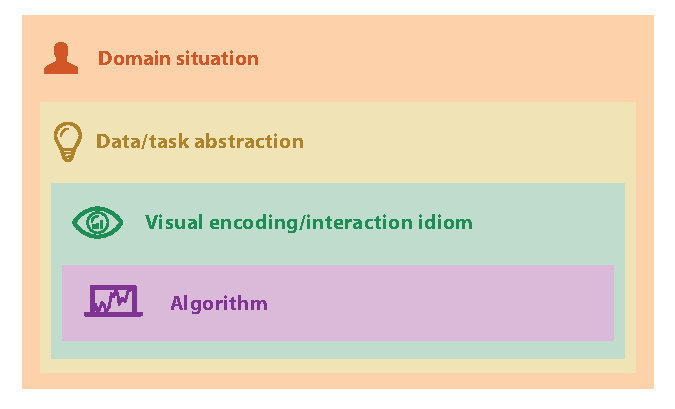
\includegraphics[width=0.75\textwidth]{figures/fig4-2.pdf}
    \caption
    [
        Munzner's nested model of visualization design.
    ]
    {
        Munzner's nested model of visualization design~\cite{Munzner2009,Munzner2014}; the arrows indicate the cascading effects of design decisions made at higher levels. Illustration: \ccLogo~E. Maguire (2014).
    }
	\centering
	\label{fig:nested-model}
\end{figure}

%-|-|-|-|-|-|-|-|-|-|-|-|-|-|-|-|-|-|-|-|-|-|-|-|-|-|-|-|-|-|-|-|-|-|-|-|-

As indicated in \autoref{intro:research-trajectory}, my personal motivation for developing an approach for classifying and abstracting tasks\index{task!task abstraction} was pragmatic: we had amassed observational data of the use of visualization tools and techniques in the interview study and field study projects, described in \autoref{ch:drvistasks} and \autoref{ch:overview} respectively, where we struggled to describe and compare tasks\index{task} performed by different people, tasks\index{task} performed with different visualization techniques or tools, as well as tasks\index{task} associated with different application domains.
We required a systematic approach for analyzing tasks\index{task!task analysis} abstractly\index{task!task abstraction}, allowing us to describe and evaluate\index{evaluation} visualization design choices that address these tasks.

\bstart{Methodology}
In \autoref{ch:typology}, we describe our comprehensive review of previous work that classified tasks\index{task}, interactions\index{interaction}, activities, and visualization design choices.
This review included over two dozen previous classification systems and theoretical frameworks from the literatures of visualization, \ac{HCI}\index{human-computer interaction (HCI)}, information retrieval\index{information retrieval}, communications\index{communications}, and cartography\index{cartography}. 
We examined the vocabulary and definitions used in this body of previous work, and after multiple rounds of coding\index{coding (qualitative data analysis)}, we had grouped similar terms, determined representative terms for each group, and arranged these representative terms into multiple levels of abstraction\footnote{\autoref{app:typology} documents the evolution of our typology.}.
We reasoned about how tasks could be described using this arrangement of terms, either in isolation, or as a sequence of interdependent tasks\index{task!task sequence}.

\bstart{Contributions}
The result of our synthesis was a typology\index{task!task typology} of abstract visualization tasks\index{task!task abstraction}, illustrated in \autoref{fig:typology}.
This typology\index{task!task typology} allows for succinct descriptions of tasks, in which a task description is comprised of {\it why}\index{{\tt why}} data is visualized (at multiple levels of abstraction), {\it what}\index{{\tt what}} dependencies a task might have in terms of {\it input}\index{{\tt input}} and {\it output}\index{{\tt output}}, and {\it how}\index{{\tt how}} the task is or can be supported in terms of visual encoding\index{visual encoding} and interaction\index{interaction} design choices; given this structure, it is possible to describe sequences of interdependent tasks\index{task!task sequence}, as illustrated in \autoref{fig:typology-dep} and in the example of \autoref{fig:typology-example}.
Our typology\index{task!task typology} has since proven to be useful in our subsequent interview study (\autoref{ch:drvistasks}), field study (\autoref{ch:overview}), and design study (\autoref{ch:emu}) projects, as well as in recent work by others; we reflect upon the adaptation and use of our typology\index{task!task typology} by others in \autoref{ch:conclusions}.

%-|-|-|-|-|-|-|-|-|-|-|-|-|-|-|-|-|-|-|-|-|-|-|-|-|-|-|-|-|-|-|-|-|-|-|-|-

\begin{figure}
    \centering
    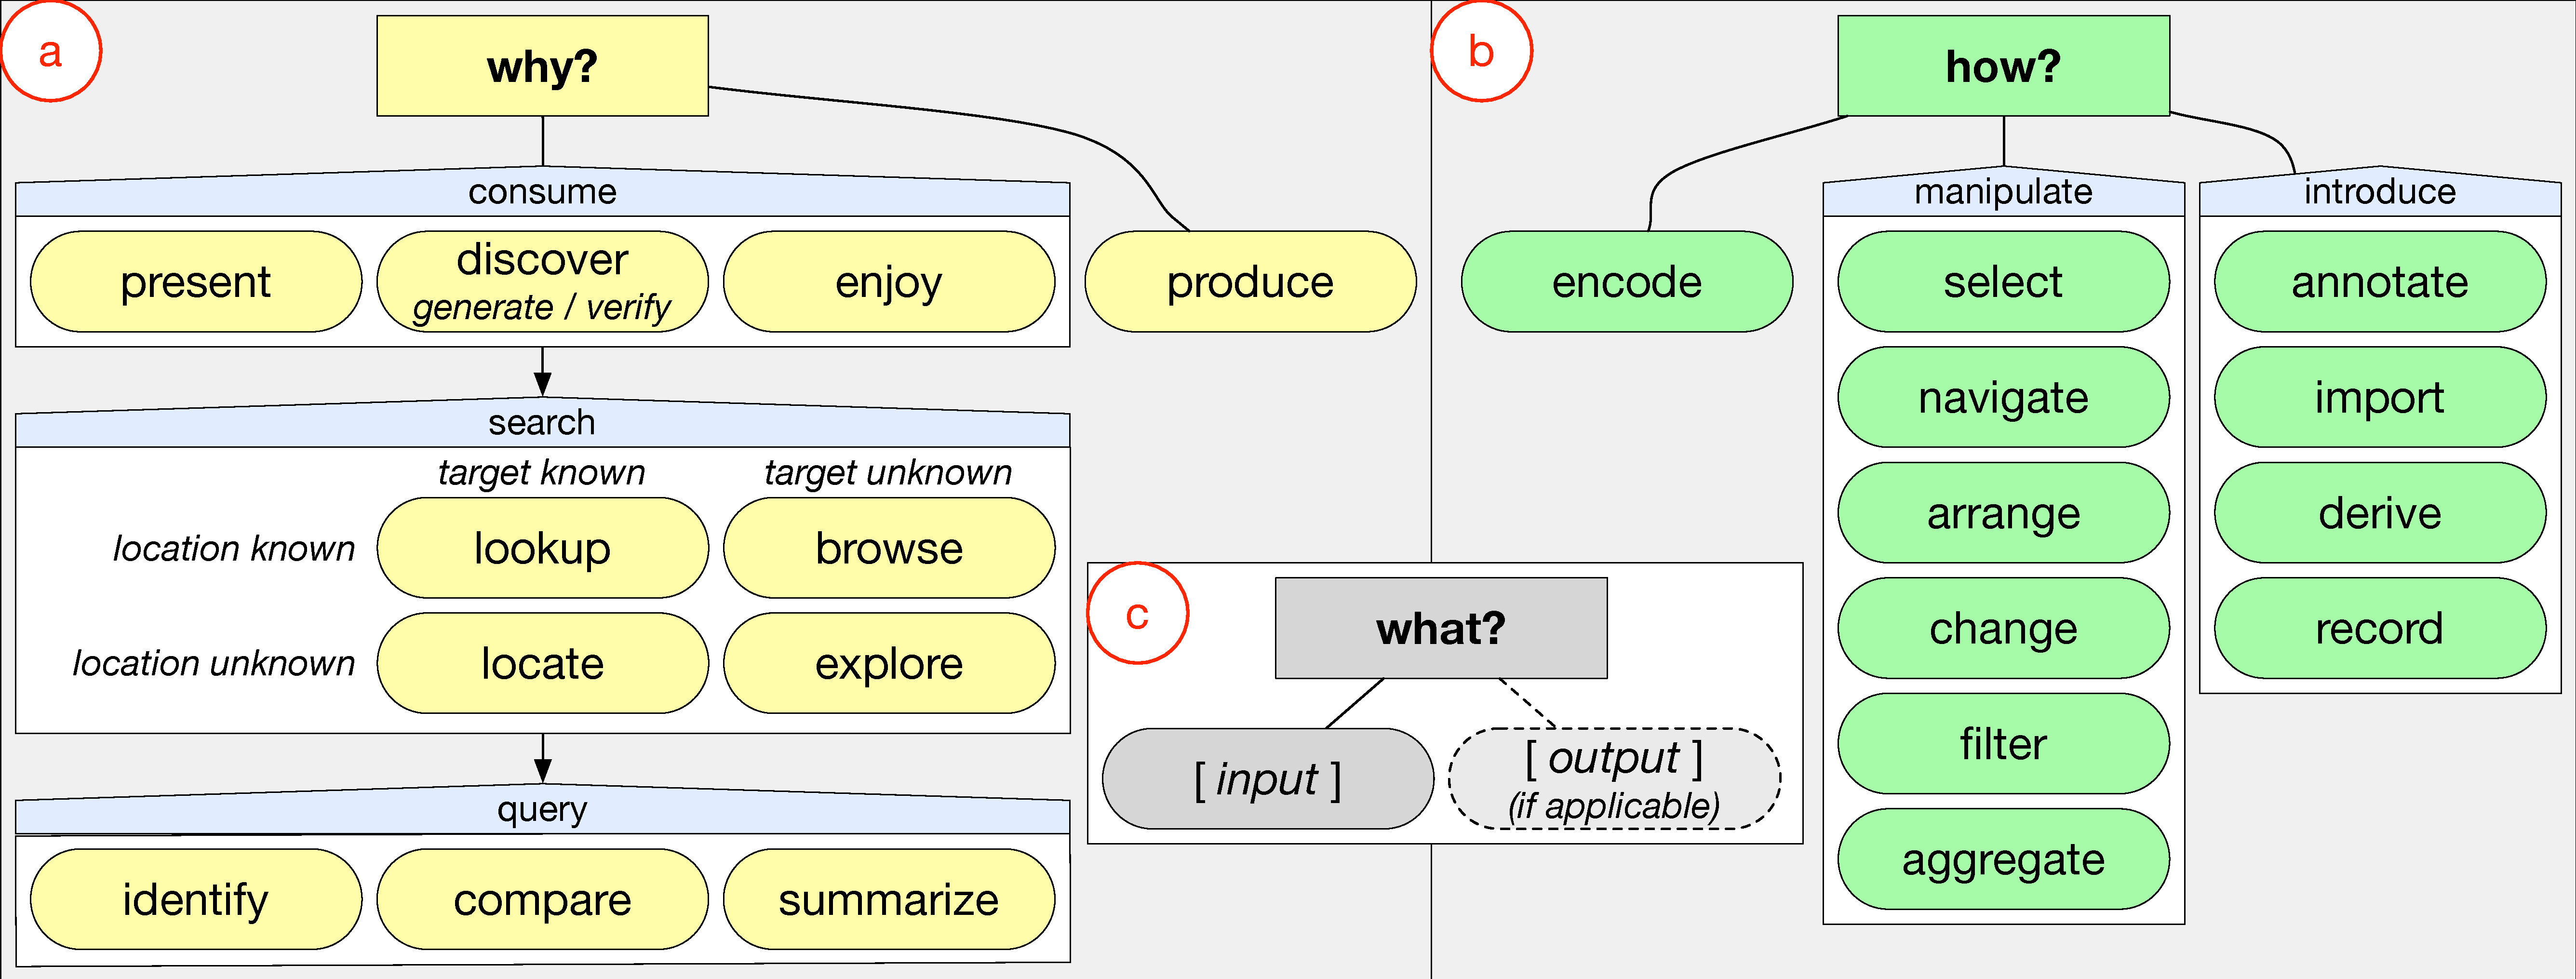
\includegraphics[width=\textwidth]{figures/typology.pdf}
    \caption
    [
        Our multi-level typology of abstract visualization tasks.
    ]
    {
        Our multi-level typology of abstract visualization tasks, which classifies  (a) {\it why} data is visualized, (b) {\it how} the task is supported in terms of visual encoding and interaction design choices, and (c) {\it what} dependencies a task might have. Note that the colors used for {\it why} and {\it how} correspond to the abstraction and technique design levels of Munzner's nested model~\cite{Munzner2009}, shown in \autoref{fig:nested-model}.
    }
    \centering
	\label{fig:typology}
\end{figure}

%-|-|-|-|-|-|-|-|-|-|-|-|-|-|-|-|-|-|-|-|-|-|-|-|-|-|-|-|-|-|-|-|-|-|-|-|-

%-|-|-|-|-|-|-|-|-|-|-|-|-|-|-|-|-|-|-|-|-|-|-|-|-|-|-|-|-|-|-|-|-|-|-|-|-

\begin{figure}
    \centering
    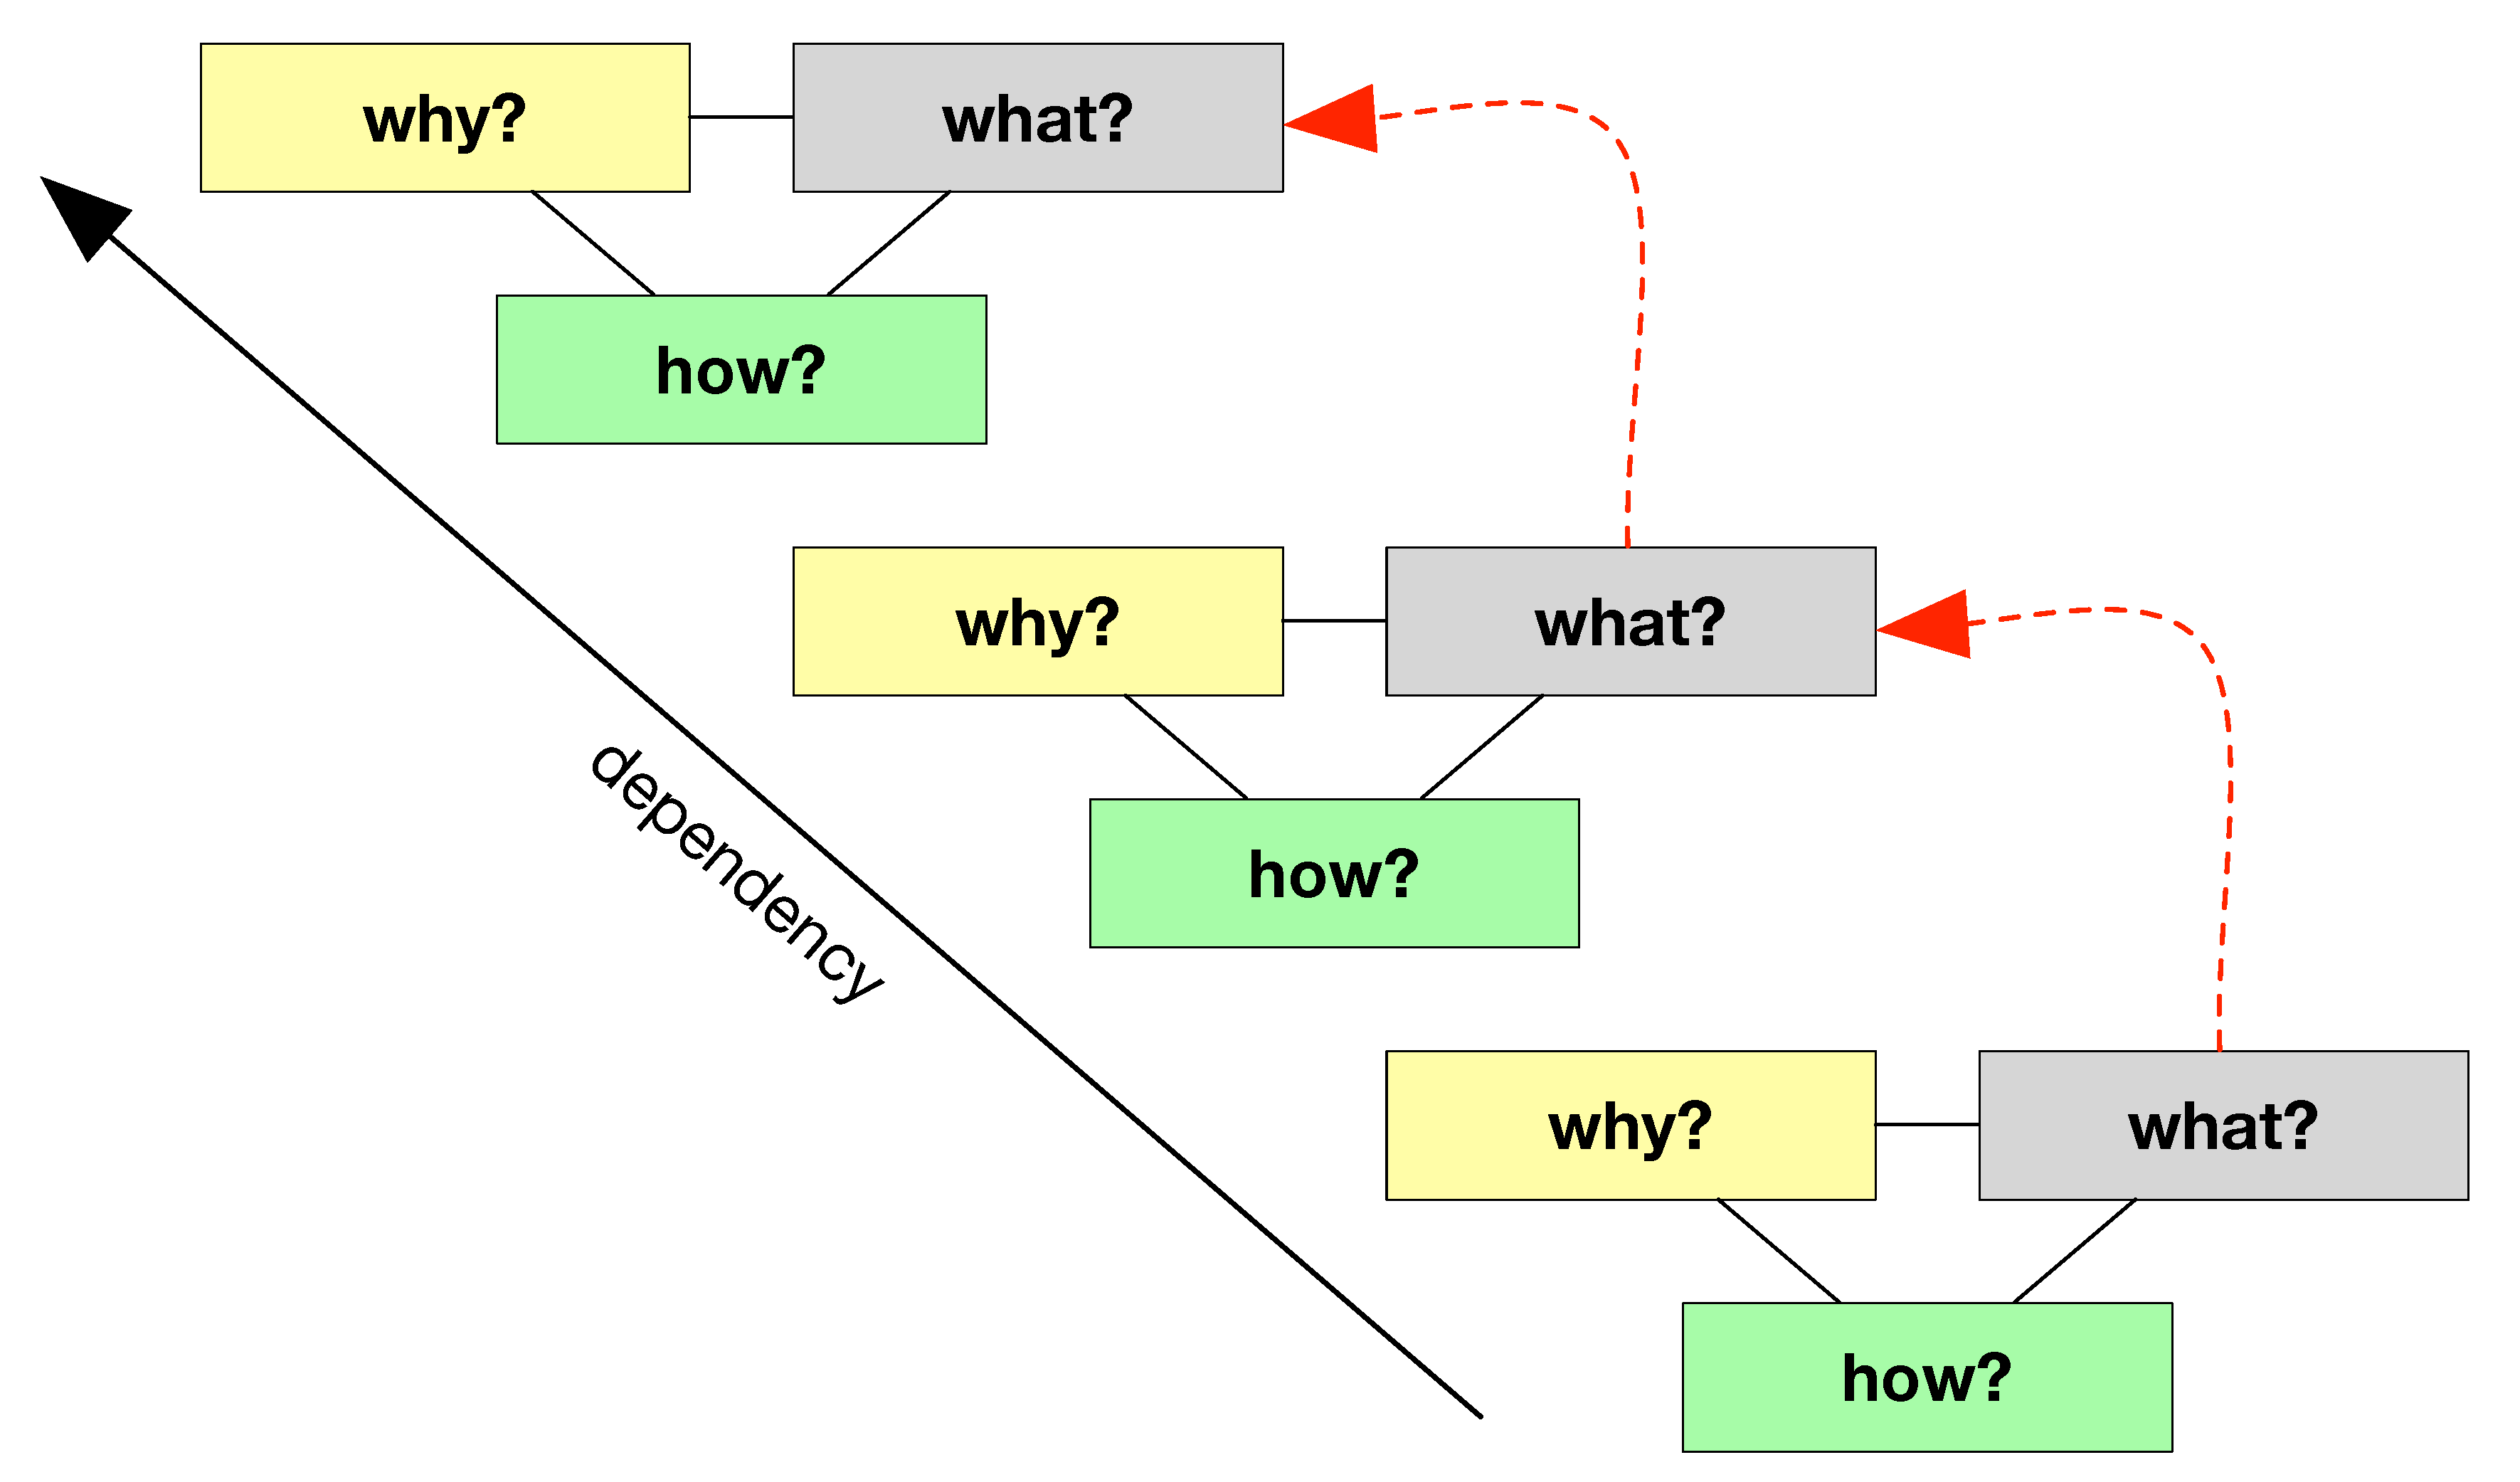
\includegraphics[width=0.75\textwidth]{figures/typology-dependency-eps-converted-to.pdf}
    \caption
    [
        Concise task descriptions using elements of the typology.
    ]{
        Concise task descriptions are constructed using elements from each part of the typology. In specifying the input and output of tasks, we can describe sequences of interdependent tasks.
    }
    \centering
    \label{fig:typology-dep}
\end{figure}

%-|-|-|-|-|-|-|-|-|-|-|-|-|-|-|-|-|-|-|-|-|-|-|-|-|-|-|-|-|-|-|-|-|-|-|-|-

%-|-|-|-|-|-|-|-|-|-|-|-|-|-|-|-|-|-|-|-|-|-|-|-|-|-|-|-|-|-|-|-|-|-|-|-|-

\begin{figure}
    \centering
    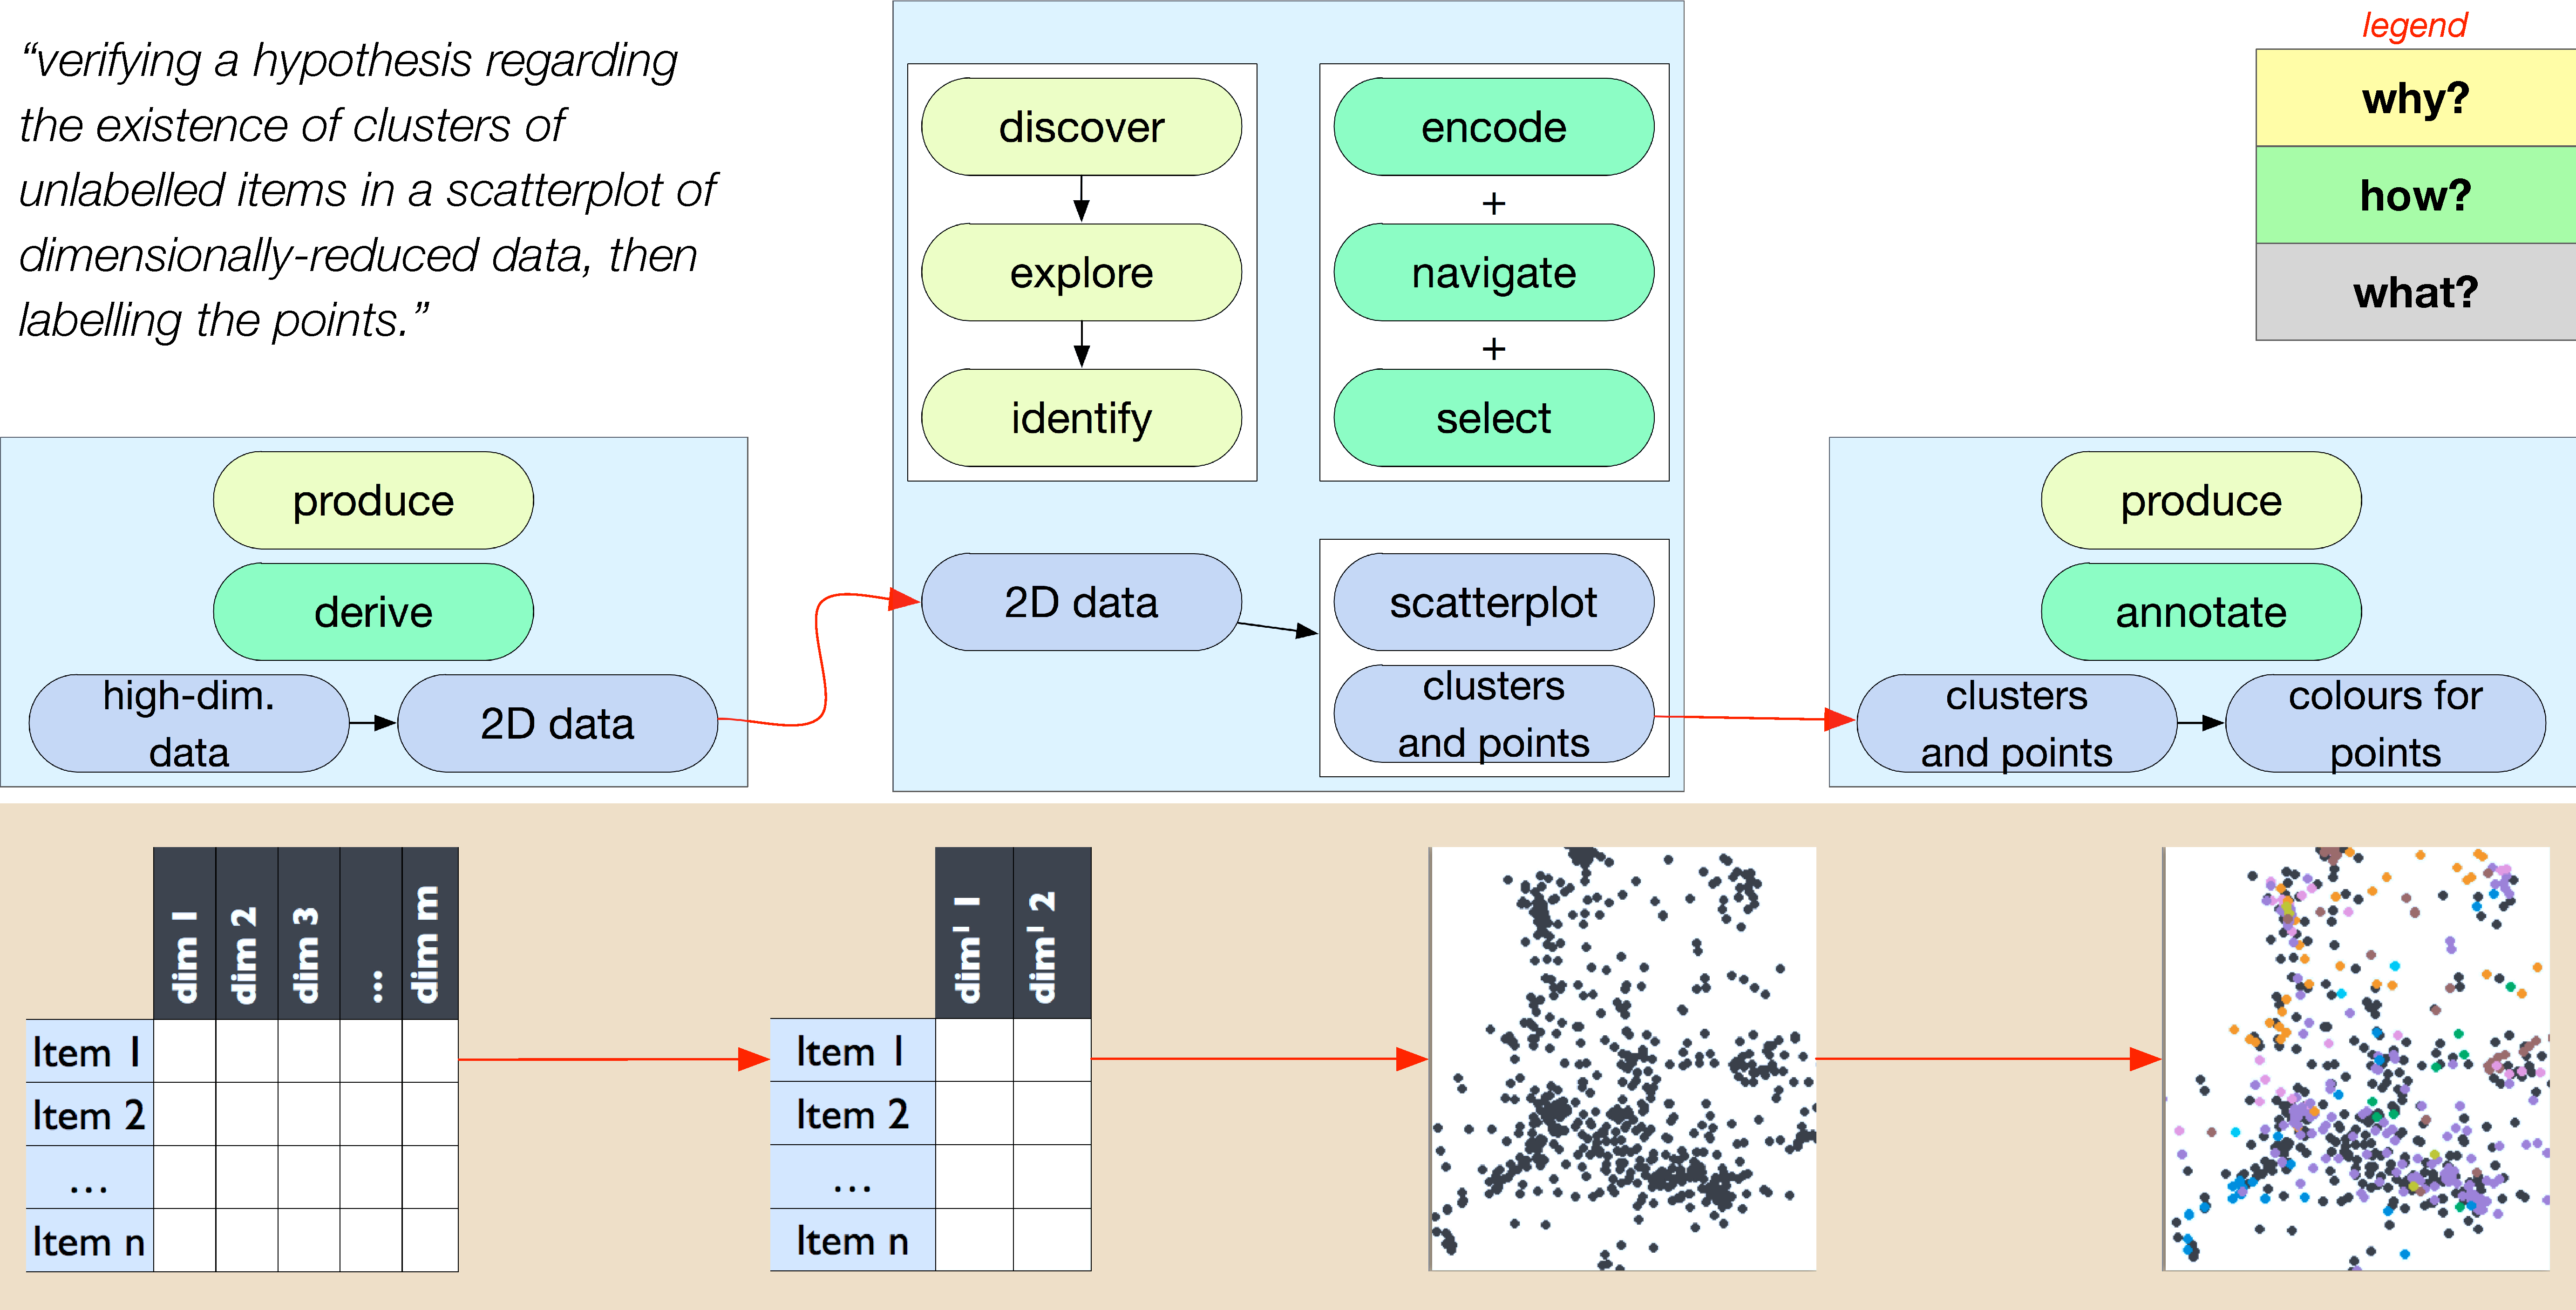
\includegraphics[width=\textwidth]{figures/typology-example-eps-converted-to.pdf}
    \caption
    [
        An example sequence of tasks using the structure and vocabulary of our typology.
    ]
    {
        An example sequence of tasks, described as a sentence (top left), as well as using the structure and vocabulary of our typology (top); the bottom depicts a series of transformations corresponding to the inputs and outputs of each task. This particular series of abstract tasks is relevant to both the interview study (\autoref{ch:drvistasks}) and field study (\autoref{ch:overview}) projects, as they both involve high-dimensional data, dimensionality reduction, and the visualization of dimensionally reduced data.
    }
    \centering
    \label{fig:typology-example}
\end{figure}

%-|-|-|-|-|-|-|-|-|-|-|-|-|-|-|-|-|-|-|-|-|-|-|-|-|-|-|-|-|-|-|-|-|-|-|-|-

%-------------------------------------------------------------------------

\subsection{Use of the Typology in an Interview Study}
\label{intro:p2}

%-------------------------------------------------------------------------

In \autoref{ch:drvistasks}, we used our typology\index{task!task typology} to {\it analyze} data analysis and the use of visualization techniques and tools ``in the wild''\index{evaluation!in the wild} by way of an interview study.
In particular, we used the typology\index{task!task typology} to examine the data analysis tasks\index{task} of individuals working in several different domains, and specifically tasks\index{task} related to the analysis of high-dimensional data\index{high-dimensional data}; we sought to better understand this data, the \ac{DR}\index{dimensionality reduction (DR)} transformations applied to it, as well as {\it why}\index{{\tt why}} and {\it how}\index{{\tt how}} visualization techniques and tools are used throughout analysts' domain-specific workflows\index{workflows}.

\bstart{Methodology}
The focus of this research was to classify the tasks associated with the visualization of dimensionally reduced data\index{dimensionality reduction (DR)}, such as in the example of \autoref{fig:typology-example}.
Our data collection and analysis methodology included twenty-four interviews with researchers and a literature survey spanning several application domains, including \ac{HCI}\index{human-computer interaction (HCI)}, chemistry\index{chemistry}, bioinformatics\index{bioinformatics}, computer science, and policy analysis\index{policy analysis}.
Our approach was similar to an interview study by \citet{Kandel2012}, one classifying data analysis and visualization among enterprise data analysts; we view our work as being complementary to their findings, given that both projects addressed data analysis and visualization ``in the wild''\index{evaluation!in the wild} for a broad group of domains.
We collected a large amount of data: diagrams, screen shots, interview notes, recordings, and transcripts, as well as interviewees' research papers, their data, and other research artifacts.

Using a qualitative coding\index{coding (qualitative data analysis)} approach, we developed a classification of task sequences\index{task!task sequence} relating to visualizing dimensionally reduced data\index{dimensionality reduction (DR)}, which are illustrated in \autoref{fig:dritw}, where each sequence\index{task!task sequence} is comprised of tasks, and each task can be defined using the vocabulary of our task typology\index{task!task typology}.
We distinguished between tasks\index{task} relating to learning about the synthetic dimensions resulting from \ac{DR} and those relating to learning about clusters of items in the dimensionally reduced data\index{dimensionality reduction (DR)}.

%-|-|-|-|-|-|-|-|-|-|-|-|-|-|-|-|-|-|-|-|-|-|-|-|-|-|-|-|-|-|-|-|-|-|-|-|-

\begin{figure}
	\centering
	\begin{subfigure}[t]{\textwidth}
	    \centering
        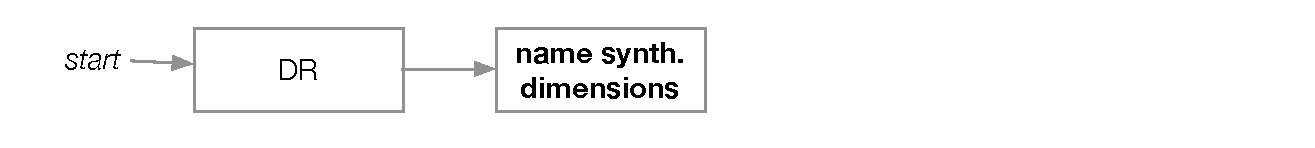
\includegraphics[height=1cm]{figures/drviztasks-name-dims.eps}
    \end{subfigure}
    ~
    \begin{subfigure}[t]{\textwidth}
	    \centering
        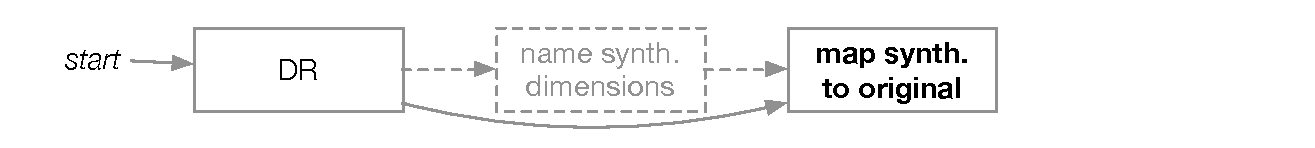
\includegraphics[height=1cm]{figures/drviztasks-map-dims.eps}
    \end{subfigure}
    ~
    \begin{subfigure}[t]{\textwidth}
	    \centering
        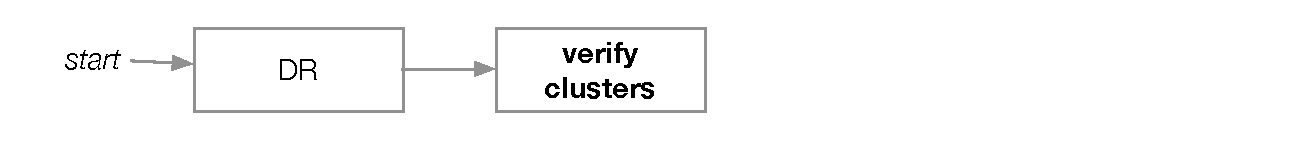
\includegraphics[height=1cm]{figures/drviztasks-identify-clusters.eps}
    \end{subfigure}
    ~
    \begin{subfigure}[t]{\textwidth}
	    \centering
        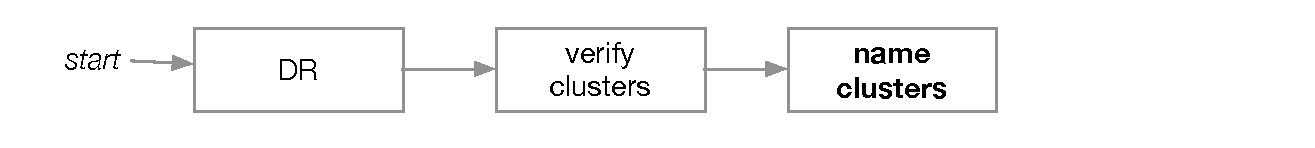
\includegraphics[height=1cm]{figures/drviztasks-name-clusters.eps}
    \end{subfigure}
    ~
    \begin{subfigure}[t]{\textwidth}
	    \centering
        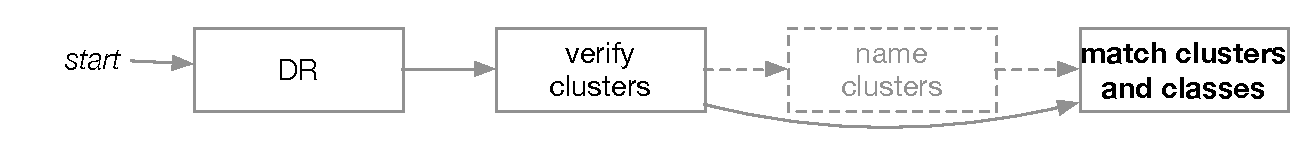
\includegraphics[height=1cm]{figures/drviztasks-match-clusters.eps}
    \end{subfigure}
	\caption
	[
	    Task sequences that involve visualizing dimensionally reduced data.
	]{
    	A classification of five task sequences that involve visualizing dimensionally reduced data, based upon findings from an interview study, documented in \autoref{ch:drvistasks}.
	}
	\centering
	\label{fig:dritw}
\end{figure}

%-|-|-|-|-|-|-|-|-|-|-|-|-|-|-|-|-|-|-|-|-|-|-|-|-|-|-|-|-|-|-|-|-|-|-|-|-

\bstart{Contributions}
With the advent of the task typology\index{task!task typology} proposed in \autoref{ch:typology}, we had a theoretical lens and vocabulary with which to approach the considerable amount of data that we collected from our interview study. 
Using the vocabulary of our typology\index{task!task typology}, %our earlier focus on dimensionality reduction can now be described using the {\it how} branch of our typology, with terms such as {\it filter}, {\it aggregate}, {\it derive}, {\it select}, and {\it annotate}. 
we were able to classify {\it why}\index{{\tt why}} these techniques are applied in sequential workflows\index{workflows}, as well as {\it what}\index{{\tt what}} the {\it inputs}\index{{\tt input}} and {\it outputs}\index{{\tt output}} of these tasks are.

\begin{sloppypar}
We contribute a {\it datatype-specific} classification of tasks grounded in observations of real-world analyst behaviour.
We encourage the further classification of tasks specific to datatype, as these are complementary to our datatype-agnostic typology\index{task!task typology} that we introduce in \autoref{ch:typology}; examples in the literature include the often-cited task by datatype taxonomy by \citet{Shneiderman1996}, classifications of graph-specific tasks~\cite{Lee2006,Saket2014}, tabular data~\cite{Henry2006}, and time-oriented data~\cite{Lammarsch2012}.
When the paper about our interview study was first published, there was no prior classification of tasks relating to visualizing dimensionally reduced data\footnote{A 2015 task taxonomy by \citet{Etemadpour2015} is discussed in \autoref{conclusions:drvistasks}.}\index{dimensionality reduction (DR)}.
The findings of our interview study and our classification of tasks is further contextualized with references to specific visual encoding\index{visual encoding} design choices; as a result, our classification of tasks can serve to validate and inform visualization technique research, a challenge that we identified in previous work~\cite{Ingram2010}.
\end{sloppypar}

%-------------------------------------------------------------------------

\subsection{Use of the Typology in a Field Study}
\label{intro:p3}

%-------------------------------------------------------------------------

In 2010, our research group began collaborating with a professional journalist who was developing a visualization tool intended for the exploration\index{{\tt explore}} of large text document collections\index{document data}.
Since this time, the tool has been deployed as {\it Overview}\footnote{\url{https://www.overviewdocs.com/}} (shown in \autoref{fig:overview}), a web-based application for investigative journalists\index{journalism} who report on large document collections\index{document data} attained from \ac{FOIA} requests or from whistleblower organizations, collections ranging in size from hundreds to tens of thousands of documents.
Between 2012 and 2014, we conducted a post-deployment field study evaluation of {\it Overview}\index{Overview (document mining tool)}, in which we analyzed its adoption\index{adoption} and self-initiated use by investigative journalists.
\autoref{ch:overview} documents this field study.

%-|-|-|-|-|-|-|-|-|-|-|-|-|-|-|-|-|-|-|-|-|-|-|-|-|-|-|-|-|-|-|-|-|-|-|-|-

\begin{figure}
    \centering
    \fbox{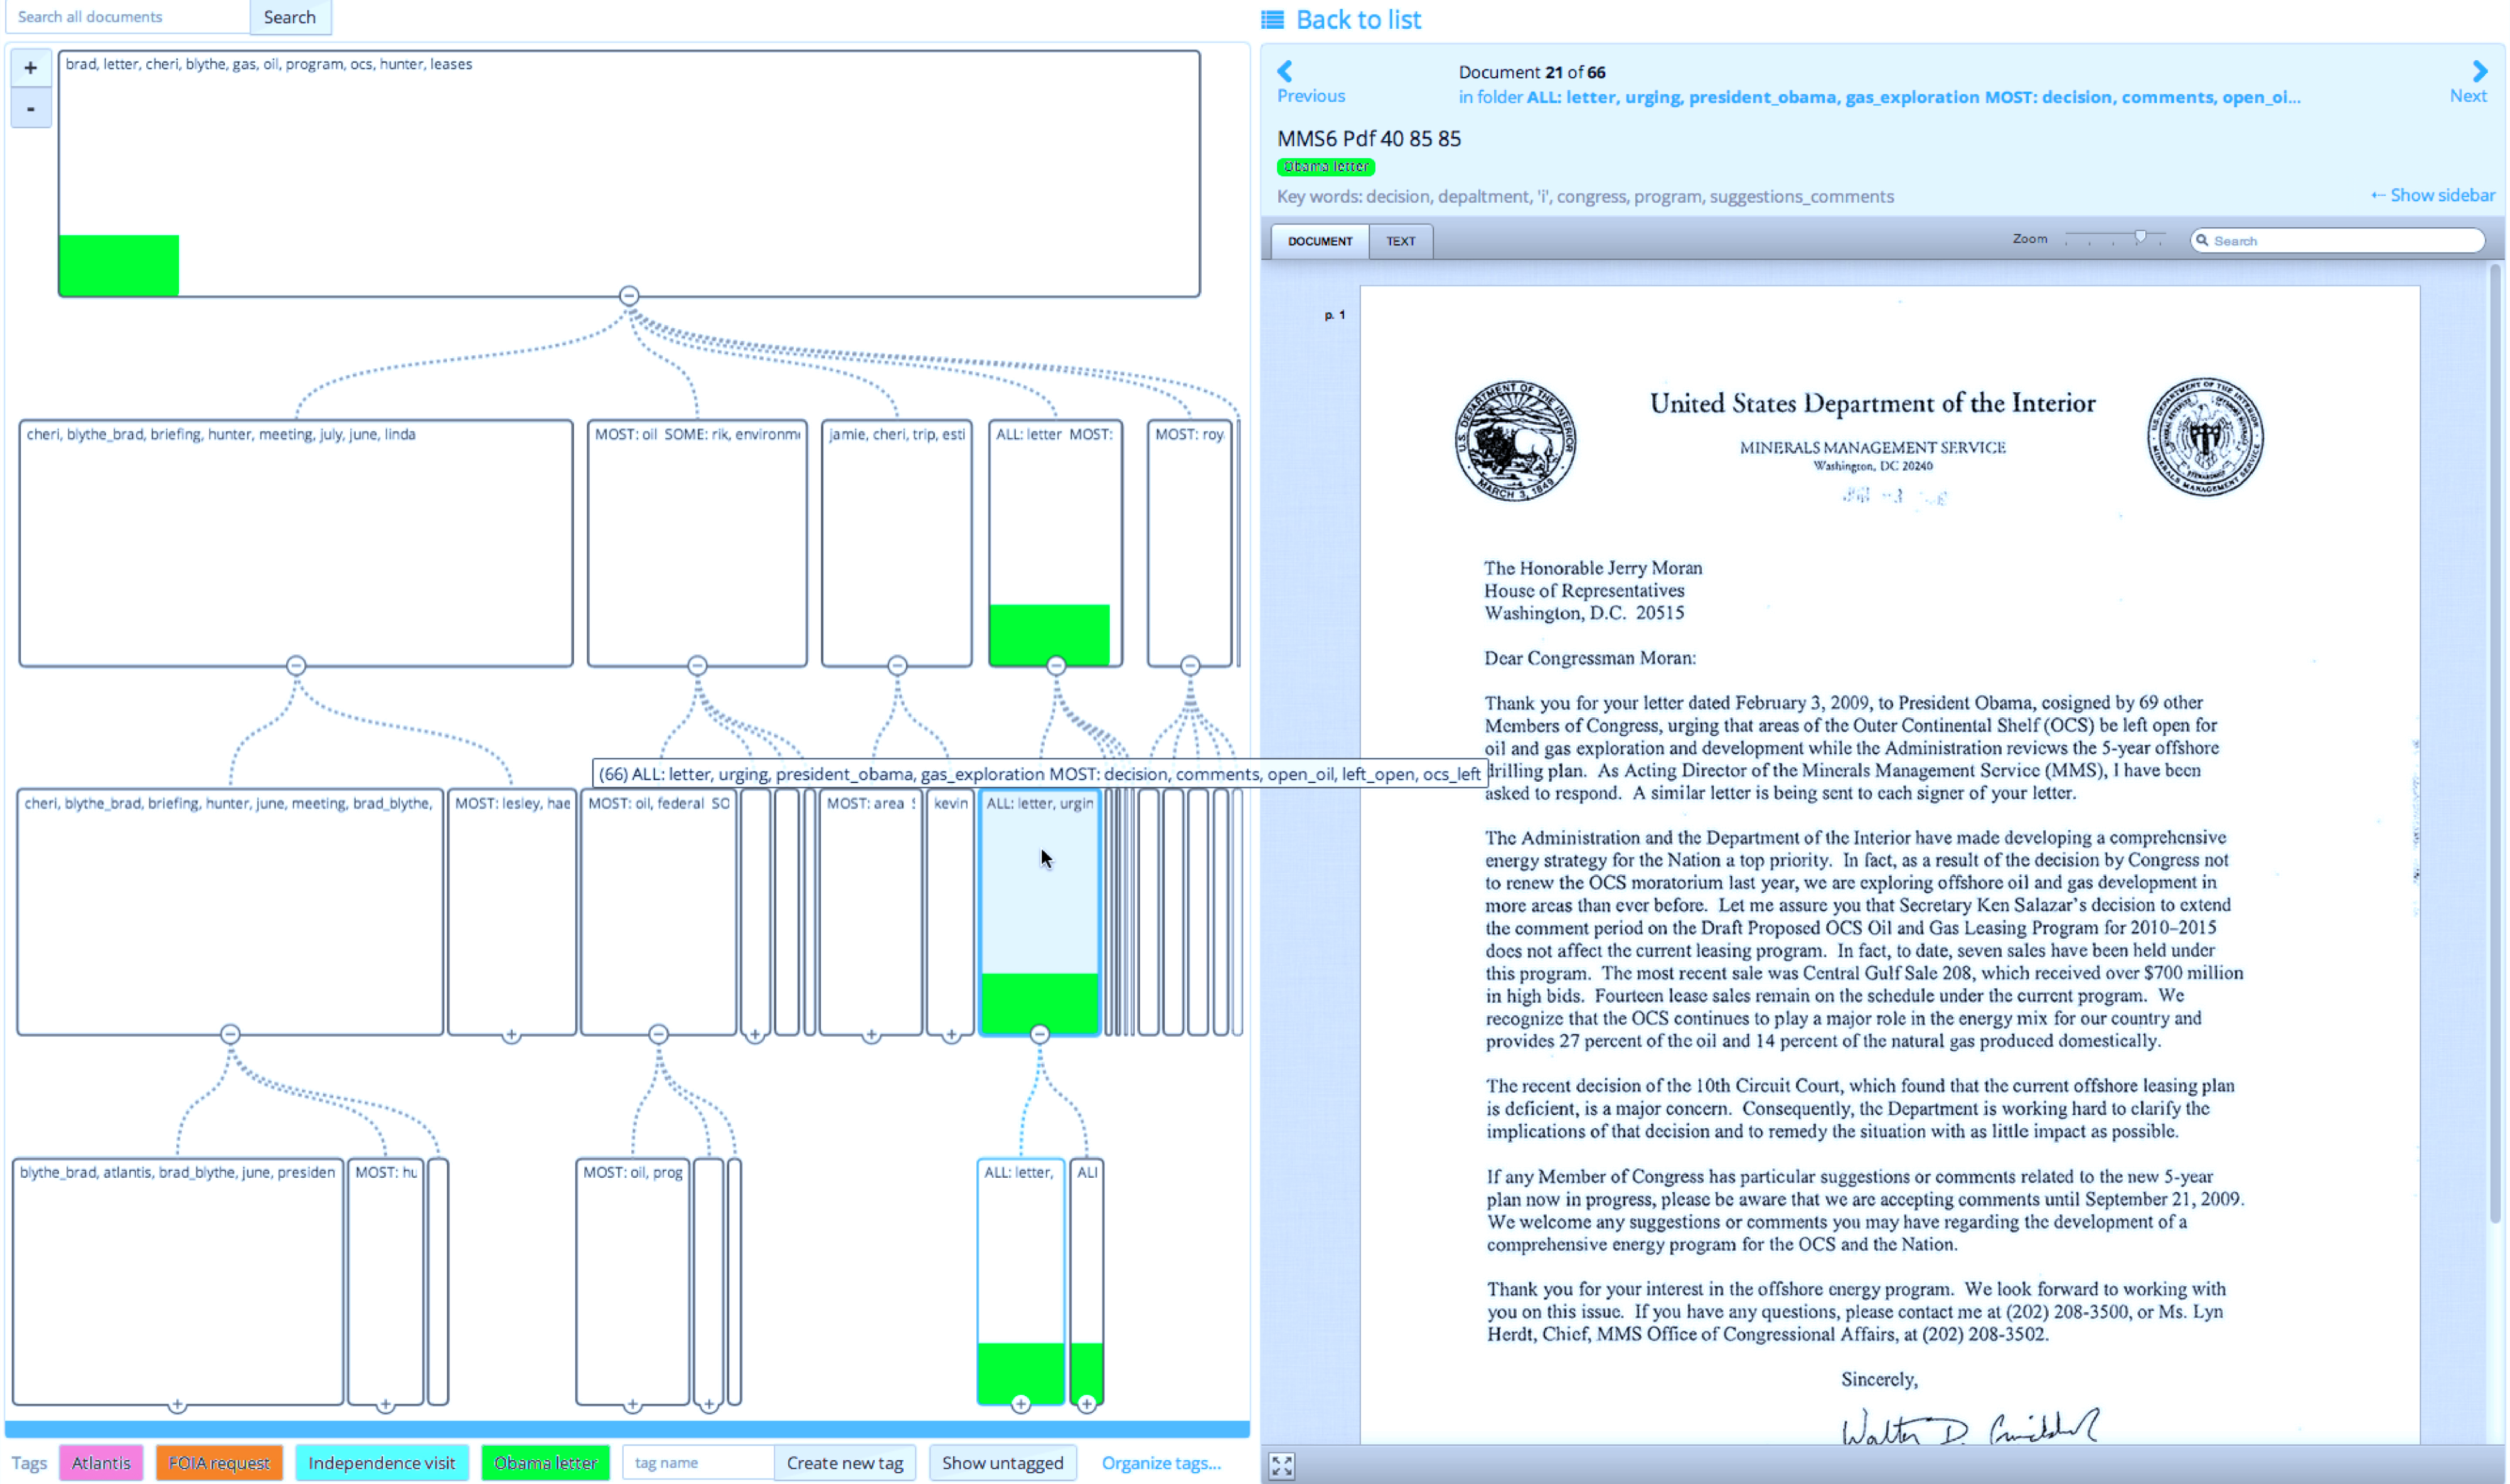
\includegraphics[width=0.975\textwidth]{figures/overview-v4-eps-converted-to.pdf}}
    \caption
    [
        {\it Overview}, a multiple-view application intended for use during an investigation of a large collection of text documents.
    ]{
        {\it Overview} is a multiple-view application intended for the systematic search, annotation, and reading of a large collection of text documents, which visualizes hierarchical clusters of documents as a tree (left). 
    }
    \centering
    \label{fig:overview}
\end{figure}

%-|-|-|-|-|-|-|-|-|-|-|-|-|-|-|-|-|-|-|-|-|-|-|-|-|-|-|-|-|-|-|-|-|-|-|-|-

\bstart{Methodology}
We conducted case studies\index{case study} of six journalists who used {\it Overview}\index{Overview (document mining tool)} to conduct investigations involving large document collections\index{document data}; in five of these cases, the investigation resulted in a published story, and one of these stories~\cite{Playford2013} was a finalist for the 2014 Pulitzer Prize in journalism\footnote{\url{http://www.pulitzer.org/2014_public_service_finalist}}.
A critical difference between our approach and other post-deployment field studies that focus on the usage of visualization tools or techniques~\cite{Lloyd2011,Saraiya2006,Shneiderman2006} is that our case study\index{case study} participants were not solicited by the researchers: they freely chose to use {\it Overview}\index{Overview (document mining tool)} and they did not inform preceding phases of design. 
We also engaged a different set of people at each stage of design, rather than the same set of people. 
This difference reflects {\it Overview}'s\index{Overview (document mining tool)} context of use: repeat usage cannot be predicted and {\it Overview}\index{Overview (document mining tool)} is only appropriate for some investigations; we have yet to encounter a journalist who specializes in investigations pertaining to large document collections\index{document data}.

We interviewed these six journalists about the form and provenance of their documents\index{document data}, the objectives of their investigation, and their use of {\it Overview}; we also collected their logged interaction data and their annotated\index{{\tt annotate}} document collections\index{document data}.
We used our task typology\index{task!task typology}, which we introduce in \autoref{ch:typology}, to better understand {\it why}\index{{\tt why}} {\it Overview}\index{Overview (document mining tool)} was adopted by these journalists to perform their investigations.

\bstart{Results}
The analysis of journalists' use of {\it Overview}\index{Overview (document mining tool)} revealed that our initial understanding of their task\index{task} was insufficient: the task\index{task} of {\it ``exploring''}\index{{\tt explore}} a document collection\index{document data}, a term that appears often in previous work on visualizing document data, is both too vague and too narrow to capture how journalists actually used {\it Overview}\index{Overview (document mining tool)}. 
% RR: p. 3. "exploring [234] or integrating insights [188] are quite abstract". Do you really mean "abstract", or do you mean "vague"? (cf. discussion of "exploring" on p. 11.) Related to this: couldn't "finding an extreme value" be abstract?  If not, what do you mean by "abstraction"? Isn't this simply independence of the details of the task?
Instead, we identified two different tasks\index{task} using the vocabulary and structure of our typology\index{task!task typology}: one of {\it generating}\index{{\tt discover}} hypotheses and {\it summarizing}\index{{\tt summarize}} the contents of a document collection, and another of {\it locating}\index{{\tt locate}} and {\it identifying}\index{{\tt identify}} specific evidence in order to {\it verify}\index{{\tt discover}} or {\it refute} prior hypotheses.

\bstart{Contributions}
Given our more precise understanding of journalists' tasks, we were able to rigorously analyze the rationale for {\it Overview}'s\index{Overview (document mining tool)} visual encoding\index{visual encoding} and interaction\index{interaction} design choices.
This analysis is transferable beyond the domain of journalism\index{journalism} and speaks to the design of visualization techniques and tools addressing document data\index{document data} and to some extent any data that can be hierarchically structured\index{hierarchical data}.
% In addition, our analysis of real world visualization usage is a form of validation for our task typology~\cite{Brehmer2013}.
Finally, we reflect upon {\it Overview}'s\index{Overview (document mining tool)} design and evaluation process, comparing our approach to previous human-centred visualization design processes~\cite{Isenberg2008,Lloyd2011}; we also discuss the value, logistics, and limitations of studying the adoption\index{adoption} of visualization techniques or tools.

%-------------------------------------------------------------------------

\subsection{Use of the Typology in a Design Study}
\label{intro:p4}

%-------------------------------------------------------------------------

In 2013, we initiated a visualization design study\index{design studies} project that provided an opportunity to validate the {\it generative} potential of our typology\index{task!task typology}.
This project was a collaboration with a company that develops energy\index{energy management} usage reporting software for multi-building organizations such as universities, school boards, or hotel chains.
Many of these client organizations have designated energy analysts who oversee large portfolios of buildings; these analysts are responsible for identifying\index{{\tt identify}} cost saving opportunities, diagnosing erratic energy usage behaviour, and attempting to understand the role of fluctuating external factors such as weather, occupancy, operating hours, and equipment usage within buildings.
Tools and techniques for addressing these tasks with respect to single buildings already exist, however they do not scale to portfolios of dozens or hundreds of buildings.
% In addition, many commercial buildings are now outfitted to report energy usage at the granularity of minutes, rather than months, which is still typical of residential buildings.
We conjectured that an interactive application integrating visualization while considering these issues of scale could address the tasks\index{task} of these analysts.
\autoref{ch:emu} documents this design study.
% A recent design study~\cite{Goodwin2013} successfully applied visualization techniques to the analysis of  modelling residential energy usage for thousands of households, which gave us hope that visualization techniques could also be applied to the analysis of large commercial building portfolios.

\bstart{Methodology}
We began by analyzing the energy domain and interviewing energy analysts from commercial client organizations who had previously used our industry partner's software, asking them about their roles and responsibilities, their technical background, their portfolio of buildings, and the limitations of current tools.
We also presented our interview findings and sought additional feedback from members of our industry partner's client services team, who have expertise with the current software and act as liaisons to client organizations.

Once again, we used our task typology\index{task!task typology}, to identify and abstract the tasks\index{task!task abstraction} of these analysts.
We narrowed our scope to tasks\index{task} that recurred often among the analysts and those that were consistent with the mandate of our industry partner's product development team to support analysis of energy consumption in building portfolios.

Over the course of four months, we designed and implemented over a dozen interactive visualization {\it data sketches}~\cite{Lloyd2011}\index{data sketch} to address the tasks\index{task} of these analysts, following a process of rapid iteration in which functional sketches featuring the analysts' data were used to further refine our understanding of their tasks\index{task} and context of use.
These data sketches\index{data sketch} were produced within the interactive interactive sandbox environment shown in \autoref{fig:pulse-cal}.
Our task abstractions\index{task!task abstraction} informed the process of mapping these tasks to a set of appropriate visual encoding\index{visual encoding} and interaction\index{interaction} design choices.
The design choices that we considered included those for performing multiple comparisons\index{{\tt compare}} between aggregate and individual items over time~\cite{Aigner2011}, for identifying\index{{\tt identify}} cyclic and acyclic events using meaningful temporal granularities~\cite{VanWijk1999}, and for identifying\index{{\tt identify}} differences in multiple lists of ranked items while simultaneously identifying the cause of rank changes~\cite{Gratzl2013}.

In early 2014, we conducted {\it chauffeured demos}~\cite{Lloyd2011}\index{chauffeured demos} of these interactive data sketches\index{data sketch} with four groups of analysts; the energy usage data used in these demos was collected from analysts' own building portfolios. 
By integrating the feedback we received on our sketches\index{data sketch} and our understanding of energy analysts' tasks\index{task}, we then envisioned ways to juxtapose\index{view coordination!view juxtaposition} and sequence\index{view coordination!view sequencing} discrete {\it views}\index{view coordination} of the data in order to support workflows\index{workflows}, and we continued to elicit feedback from analysts and our collaborators' client services team.

%-|-|-|-|-|-|-|-|-|-|-|-|-|-|-|-|-|-|-|-|-|-|-|-|-|-|-|-|-|-|-|-|-|-|-|-|-

\begin{figure}
    \centering
    \fbox{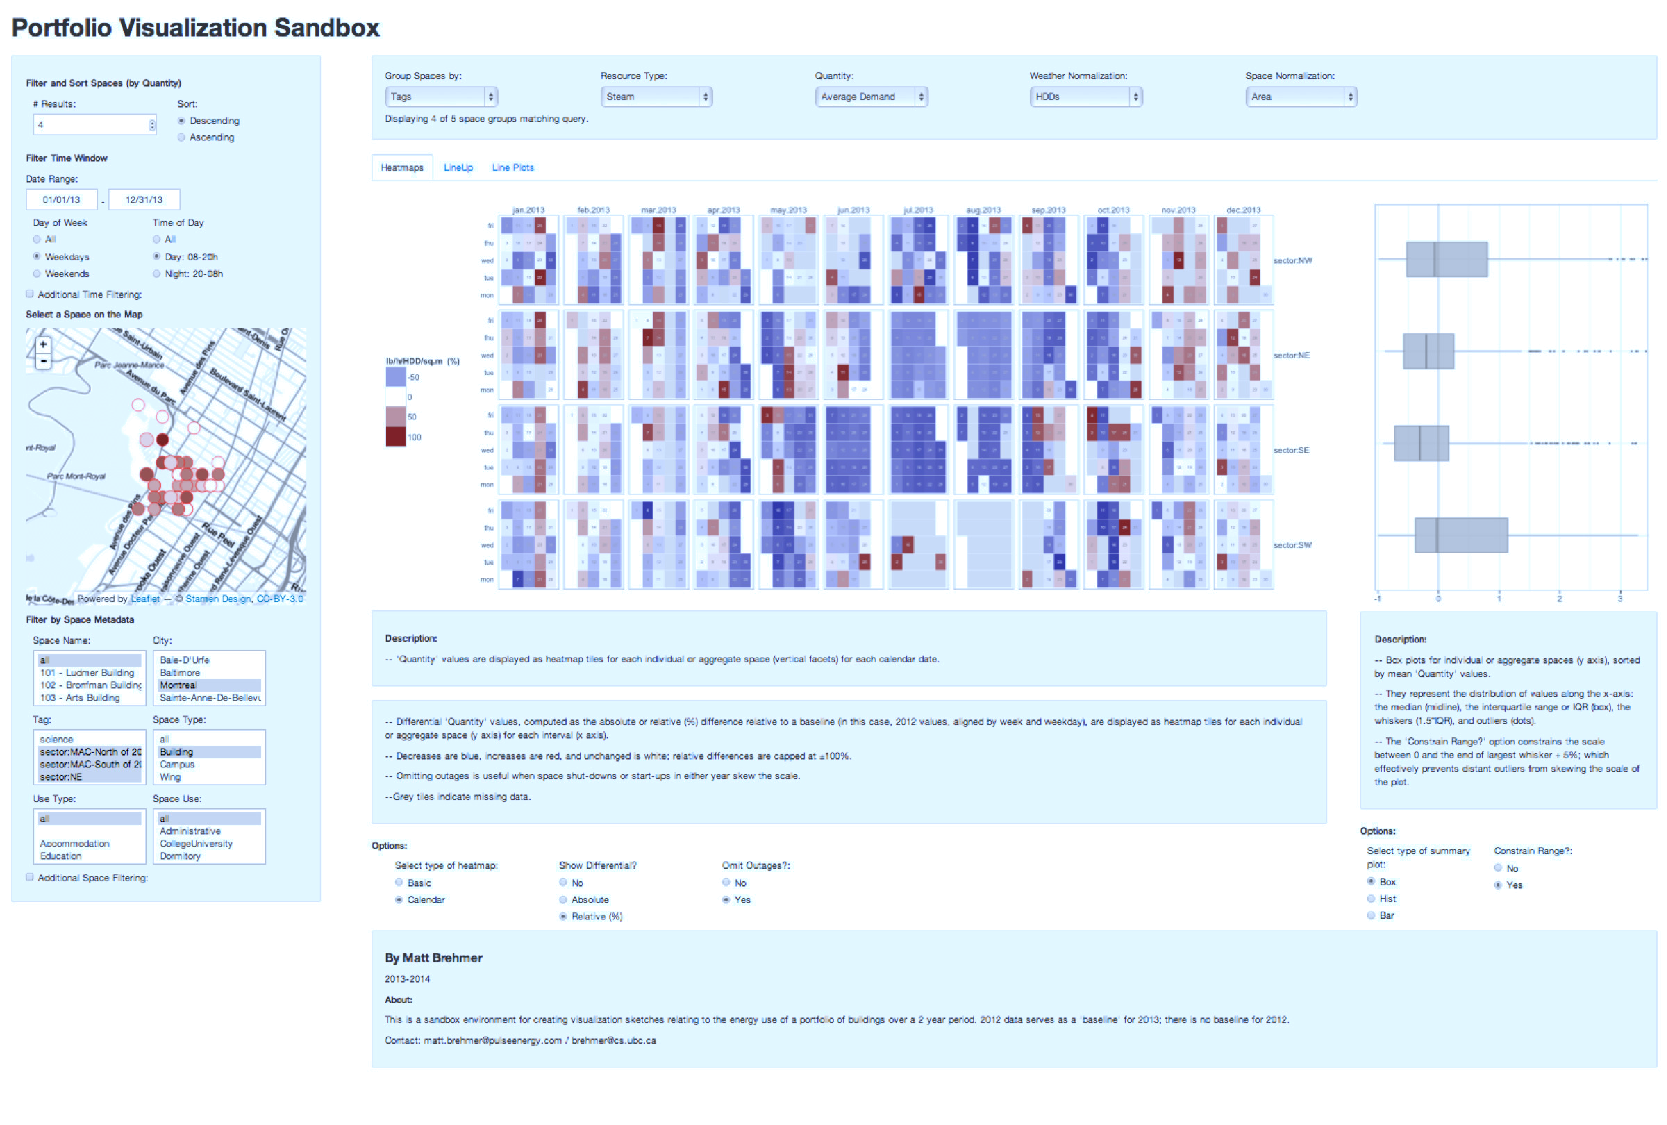
\includegraphics[width=0.975\textwidth]{figures/pulse-cal-eps-converted-to.pdf}}
    \caption
    [
         A sandbox environment for creating visualization data sketches pertaining to energy portfolio analysis.
    ]{
        A sandbox environment for creating visualization data sketches pertaining to the analysis of energy usage in large building portfolios. In this visualization data sketch, a calendar-based time series matrix is juxtaposed with summary boxplots, where each row is a group of buildings. Both the matrix and the boxplots encode the difference between average energy demand in 2012 and 2013.
    }
    \label{fig:pulse-cal}
    \centering
\end{figure}

%-|-|-|-|-|-|-|-|-|-|-|-|-|-|-|-|-|-|-|-|-|-|-|-|-|-|-|-|-|-|-|-|-|-|-|-|-

\bstart{Results}
Our collaborators have since adopted\index{adoption} a number of our designs into a new version of their commercial energy analysis software tool.
They assigned over ten full-time software developers to the project since mid-2014 and the tool has since been released to some client organizations in a small pilot deployment; the tool will soon\footnote{Relative to November 2015.} be deployed to thousands of other clients.

\bstart{Contributions}
As a result of abstracting the data and tasks\index{task!task abstraction} relating to the energy management\index{energy management} domain, visualization practitioners working in other domains might benefit from our classification of matches and mismatches between abstract tasks\index{task!task abstraction} and visualization design choices, particularly for domains that involve comparing\index{{\tt compare}} many concurrent time series\index{time-oriented data}.

We also confronted issues of domain convention\index{domain convention} in this project; in the energy sector, some visual encodings\index{visual encoding} carry very specific meanings. 
We considered how to introduce unfamiliar\index{familiarity} visual encodings\index{visual encoding} and how to get people working in this domain to trust\index{trust} them.

Finally, we contribute some methodological guidance for visualization design studies\index{design studies}, including our approach to work domain analysis\index{work domain analysis}, a systematic task analysis\index{task!task analysis} and abstraction\index{task!task abstraction}, our sandbox prototyping and workflow\index{workflows} design, as well as how to effectively present visualization design documentation.

%-------------------------------------------------------------------------

\subsection{Summary of Contributions}
\label{intro:contrib-summary}

%-------------------------------------------------------------------------

The contributions of this dissertation can be summarized as follows:

\begin{itemize}
    \item A typology\index{task!task typology} of abstract visualization tasks\index{task}, which allows for succinct descriptions of tasks and task sequences\index{task!task sequence} in terms of {\it why}\index{{\tt why}} data is visualized, {\it what}\index{{\tt what}} dependencies a task might have in terms of {\it input}\index{{\tt input}} and {\it output}\index{{\tt output}}, and {\it how}\index{{\tt how}} the task is supported in terms of visual encoding\index{visual encoding} and interaction\index{interaction} design choices (\autoref{ch:typology}).
    \item A synthesis of the literature relating to visualization tasks\index{task} (\autoref{ch:typology}).
    \item A datatype-specific classification of five task sequences\index{task!task sequence} relating to visualizing dimensionally reduced data\index{dimensionality reduction (DR)}, one based on findings from our interview study with data analysts spanning several application domains. This classification draws upon and demonstrates the descriptive power of our typology of tasks\index{task!task typology} and is intended to inform the design of new tools and techniques for visualizing dimensionally reduced data\index{dimensionality reduction (DR)} (\autoref{ch:drvistasks}).
    \item A field study evaluation of {\it Overview}\index{Overview (document mining tool)}, a visualization tool for investigating large text document collections\index{document data}. We draw upon and demonstrate the descriptive and evaluative power of our typology of tasks\index{task!task typology} and characterized two abstract tasks relating to document mining\index{document mining} (\autoref{ch:overview}). 
    \item Seven lessons relating to the design of interactive visualization tools for hierarchical data\index{hierarchical data} and document data\index{document data} in particular. These lessons are based on an analysis of successive deployed versions of {\it Overview}\index{Overview (document mining tool)} and its adoption\index{adoption} by self-initiated journalists\index{journalism} (\autoref{ch:overview}).
    \item A methodological reflection on the study of visualization adoption\index{adoption} (\autoref{ch:overview}).
    \item A demonstration of the descriptive, evaluative, and generative power of our typology of tasks\index{task!task typology} in a visualization design study\index{design studies} within the energy domain (\autoref{ch:emu}).
    \item An identification of matches and mismatches between visualization design choices and three abstract tasks for concurrent time series data\index{time-oriented data} (\autoref{ch:emu}).
    \item Two lessons pertaining to familiarity\index{familiarity} with visual encodings\index{visual encoding}, two lessons pertaining to the trust\index{trust} of data aggregation design choices\index{{\tt aggregate}}, and three lessons pertaining to visualization design methodology (\autoref{ch:emu}).
\end{itemize}

%-------------------------------------------------------------------------
%-------------------------------------------------------------------------

\section{Extension and Impact of the Typology}
\label{intro:adoption}

%-------------------------------------------------------------------------
%-------------------------------------------------------------------------

In \autoref{ch:conclusions}, we comment on how our task typology was subsequently extended by Munzner in her 2014 book {\it Visualization Analysis and Design}~\cite{Munzner2014}; this modified typology is shown in \autoref{fig:typology-extension}.
Munzner moved {\it introduce} nodes from the {\it how} part of the typology to become forms of {\it produce} in the {\it why} part of the typology; she also added {\it targets} to the {\it why} part of the typology, referring to the original {\it why} part of our typology as {\it actions}; finally, she reorganized the {\it how} part of the typology and elaborated on forms of {\it encode}.
We explicitly make reference to and use Munzner's modifications to the typology\index{task!task typology} in our interview study  (\autoref{ch:drvistasks}) and in our design study ({\autoref{ch:emu}).
\autoref{ch:conclusions} also contains commentary on the origin, the benefits, and the potential drawbacks of Munzner's modifications.

We also present a survey of how our task typology\index{task!task typology} and our approach to systematically analyzing and abstracting tasks has been used and/or extended by others in the visualization community, including how our typology\index{task!task typology} may integrate with novel theoretical frameworks.
This survey includes the use of our typology\index{task!task typology} to analyze domain-specific usage of visualization techniques or tools, from bioinformatics\index{bioinformatics} to malware analysis, as well as datatype-specific visualization usage, from geospatial data to multiplex networks.
This survey also includes the use of our typology\index{task!task typology} to specify and contextualize tasks in experimental studies, as well as the use of our typology\index{task!task typology} to motivate the design of novel visualization techniques and tools.

%-|-|-|-|-|-|-|-|-|-|-|-|-|-|-|-|-|-|-|-|-|-|-|-|-|-|-|-|-|-|-|-|-|-|-|-|-

\begin{figure}
	\centering
	\begin{subfigure}[t]{0.48\textwidth}
	    \centering
        \fbox{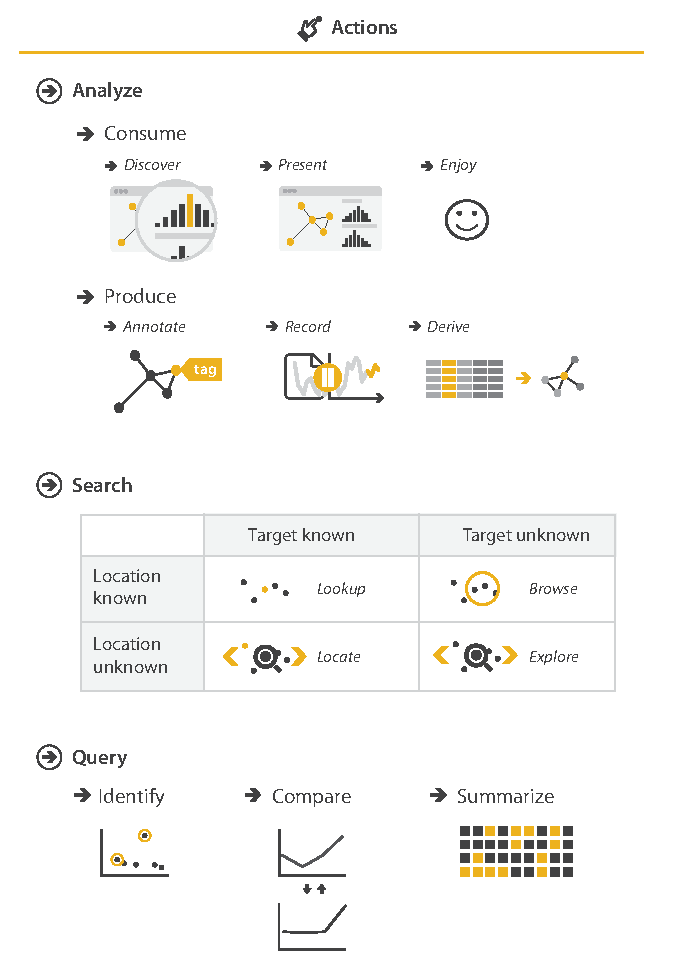
\includegraphics[height=7.75cm]{figures/fig3-2.pdf}}
        \caption{{\it why} ({\it actions}).}
    \end{subfigure}
    ~
    \begin{subfigure}[t]{0.48\textwidth}
	    \centering
        \fbox{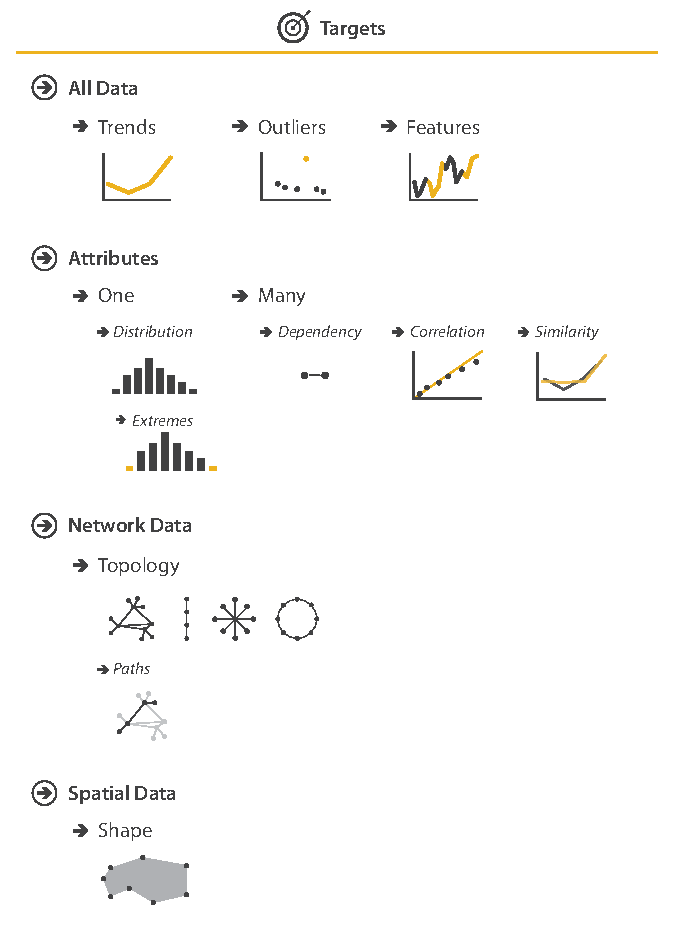
\includegraphics[height=7.75cm]{figures/fig3-6.pdf}}
        \caption{{\it why} ({\it targets}).}
    \end{subfigure}
    ~
    \begin{subfigure}[t]{\textwidth}
	    \centering
        \fbox{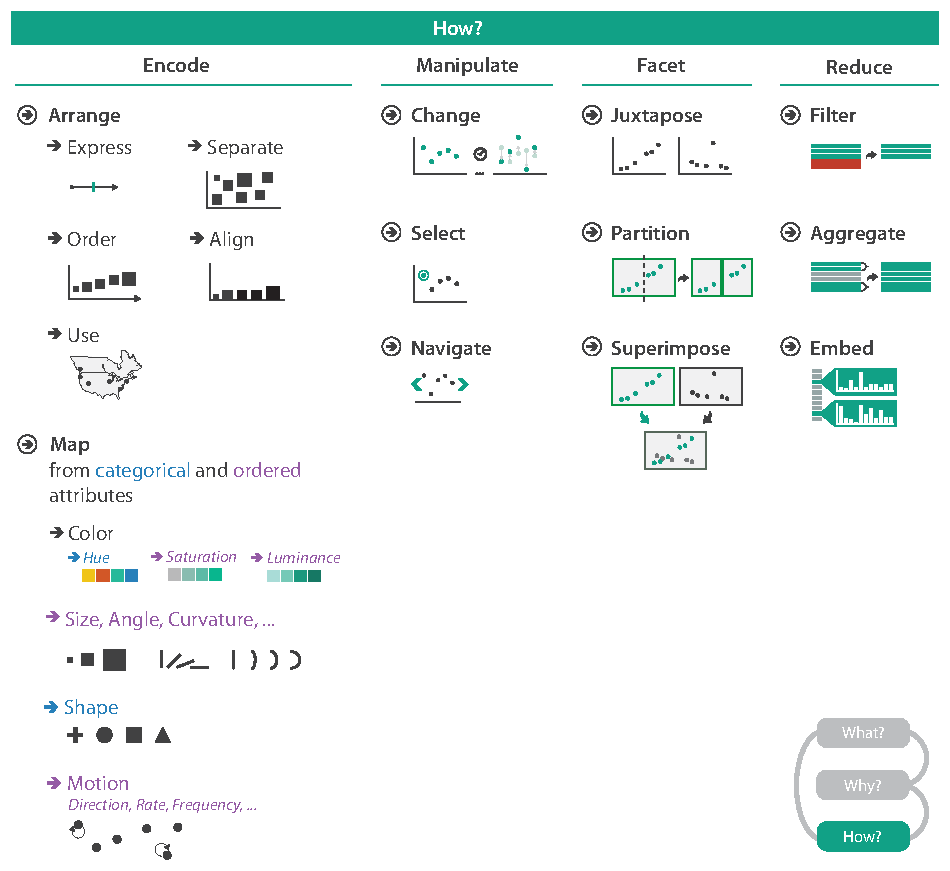
\includegraphics[height=7cm]{figures/fig3-7.pdf}}
        \caption{{\it how} (design choices).}
    \end{subfigure}
	\caption
	[
	    A modified version of our typology appearing in \citet{Munzner2014}.
	]{
    	A modified version of our typology appearing in \citet{Munzner2014} (\cf \autoref{fig:typology}): (a) forms of {\it produce} were moved from {\it how}; (b) a new classification of {\it targets}; (c) a reorganization of {\it how}. Illustrations: \ccLogo~E. Maguire (2014).
	}
	\centering
	\label{fig:typology-extension}
\end{figure}

%-|-|-|-|-|-|-|-|-|-|-|-|-|-|-|-|-|-|-|-|-|-|-|-|-|-|-|-|-|-|-|-|-|-|-|-|-

%-------------------------------------------------------------------------
%-------------------------------------------------------------------------
\section{A Note on Chronology}
\label{intro:chronology}

%-------------------------------------------------------------------------
%-------------------------------------------------------------------------

The duration of the projects described in this dissertation extended long periods of time.
As a result, periods of focused research on these projects were interleaved or overlapping.
\autoref{fig:thesis-timeline} illustrates the chronological history of these projects, indicating the core focus periods of projects, important milestones, as well as periods of part-time focus.
\autoref{fig:thesis-timeline} also indicates other milestones in my PhD, research projects not included in this dissertation~\cite{Brehmer2014a,Fulda2015}, and internships.

%-|-|-|-|-|-|-|-|-|-|-|-|-|-|-|-|-|-|-|-|-|-|-|-|-|-|-|-|-|-|-|-|-|-|-|-|-

\begin{figure}
    \centering
    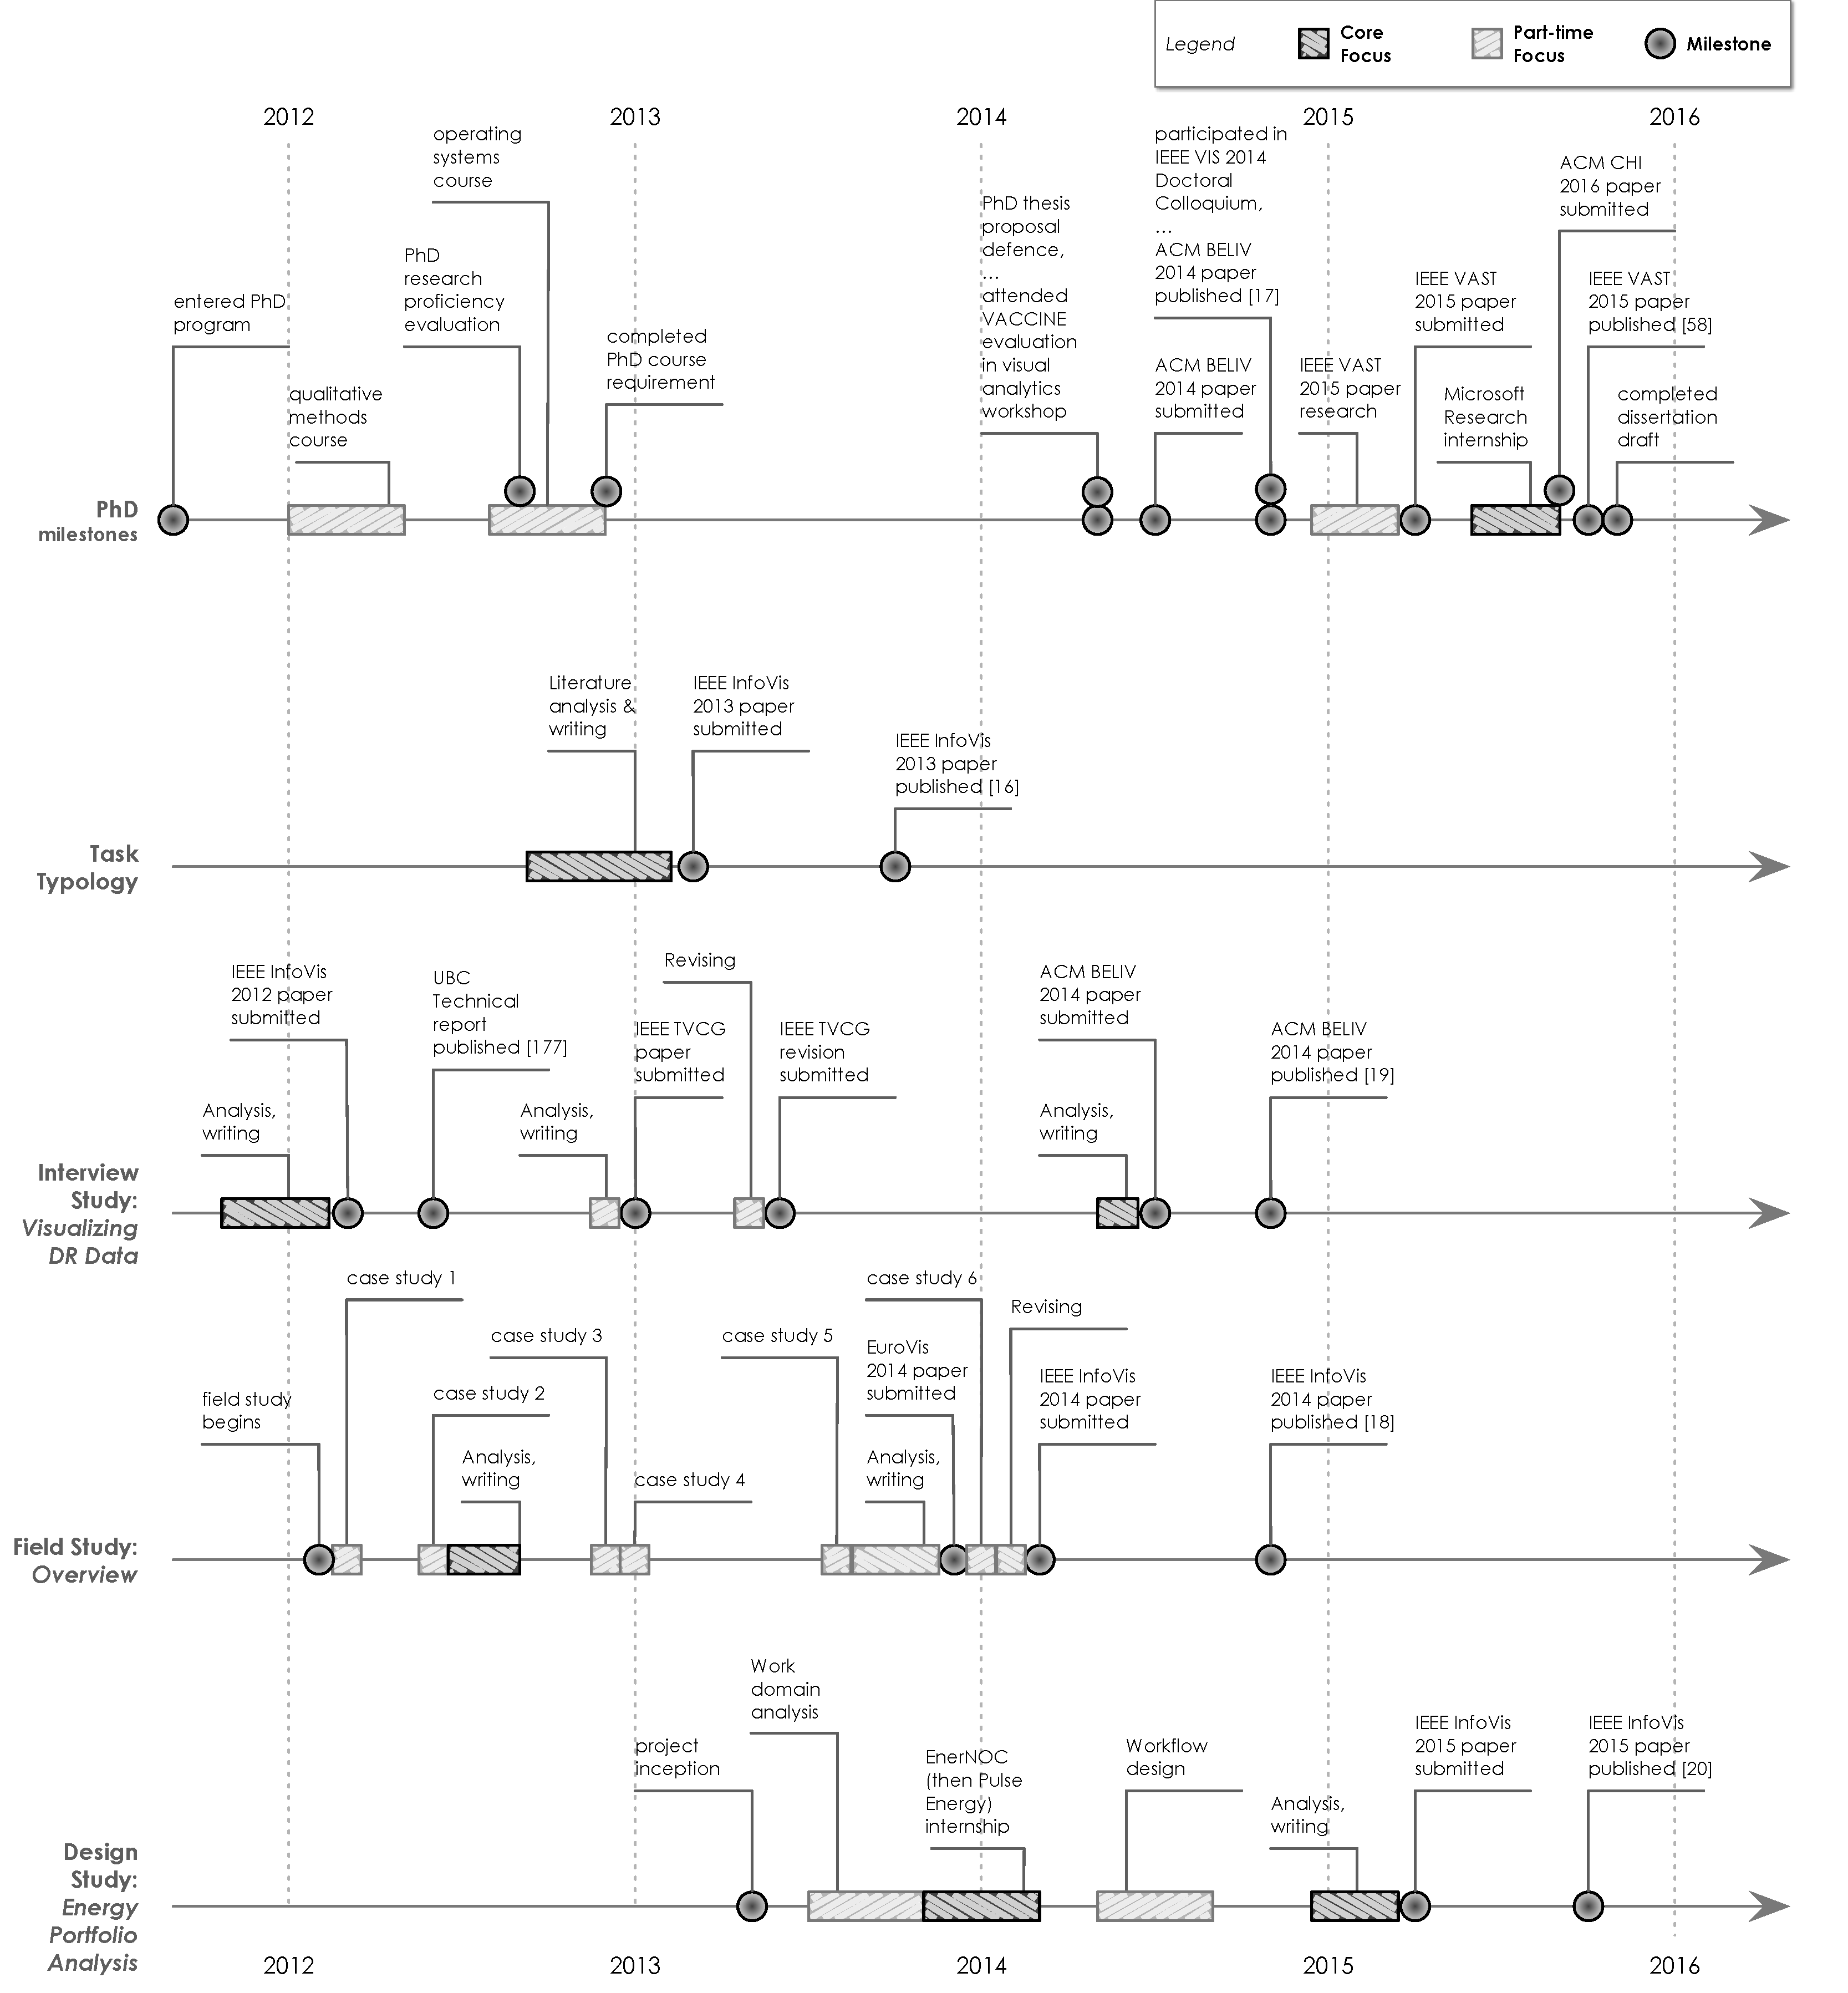
\includegraphics[width=\textwidth]{figures/thesis-timeline.pdf}
    \caption
    [
        Timelines of the projects described in this dissertation.
    ]{
        Timelines of the projects described in this dissertation. Note that the projects described in this dissertation overlapped in time. While the order of the chapters in this dissertation reflect the order in which the projects were completed, they do not reflect the order in which they were initiated.
    }
    \label{fig:thesis-timeline}
    \centering
\end{figure}

%-|-|-|-|-|-|-|-|-|-|-|-|-|-|-|-|-|-|-|-|-|-|-|-|-|-|-|-|-|-|-|-|-|-|-|-|-

\endinput


%    2. Main body
% Generally recommended to put each chapter into a separate file
%-------------------------------------------------------------------------
%-------------------------------------------------------------------------
%-------------------------------------------------------------------------

\chapter{A Typology of Abstract Visualization Tasks}
\label{ch:typology}

%-------------------------------------------------------------------------
%-------------------------------------------------------------------------
%-------------------------------------------------------------------------

\begin{epigraph}
    \item \emph{``By thinking about visualization as a process instead of an outcome, we arm ourselves with an incredibly powerful thinking tool.''} ---~Jer Thorp in ``Visualization as process, not output''~\cite{Thorp2013} (\emph {Harvard Business Review}, April 3, 2013)
\end{epigraph}

\footnote{This chapter is a slightly modified version of our paper {\it A Multi-Level Typology of Abstract Visualization Tasks} by Matthew Brehmer and Tamara Munzner; in IEEE Transactions on Visualization and Computer Graphics (Proceedings of InfoVis 2013), 19(12), p. 2376--2385~\cite{Brehmer2013}. \url{http://dx.doi.org/10.1109/TVCG.2013.124}.}The considerable previous work characterizing visualization processes has focused on low-level tasks\index{task!low-level tasks} or interactions\index{interaction} and high-level tasks\index{task!high-level tasks}, leaving a gap between them that is not addressed\footnote{Referring to the examples cited in \autoref{intro:research-trajectory}, {\it finding an extreme value}~\cite{Amar2005} is an example of a low level of abstraction while {\it exploring}~\cite{Yi2007} or {\it integrating insights}~\cite{Springmeyer1992}\index{insight} are examples of a higher level of abstraction.}.
% RR: p. 3. "exploring [234] or integrating insights [188] are quite abstract". Do you really mean "abstract", or do you mean "vague"? (cf. discussion of "exploring" on p. 11.) Related to this: couldn't "finding an extreme value" be abstract?  If not, what do you mean by "abstraction"? Isn't this simply independence of the details of the task?
This gap leads to a lack of distinction between the ends\index{task!ends} and means\index{task!means} of a task\index{task}, limiting the potential for rigorous analysis.
We contribute a multi-level typology\index{task!task typology} of visualization tasks\index{task} to address this gap, distinguishing {\it why}\index{{\tt why}} and {\it how}\index{{\tt how}} a visualization task\index{task} is performed, as well as {\it what}\index{{\tt what}} the task\index{task} inputs\index{{\tt input}} and outputs\index{{\tt output}} are.
Our typology\index{task!task typology} allows complex tasks\index{task} to be expressed as sequences of interdependent tasks\index{task!task sequence}, resulting in concise and flexible descriptions for tasks\index{task} of varying complexity and scope.
It provides abstract rather than domain-specific descriptions of tasks\index{task}, so that useful comparisons can be made between visualization techniques or tools targeted at different application domains.
This descriptive power supports a level of analysis required for the generation of new designs, by guiding the translation of domain-specific problems into abstract tasks\index{task!task abstraction}, and for the qualitative evaluation\index{evaluation} of visualization tools or techniques.
We demonstrate the benefits of our approach in a detailed example, comparing task\index{task} descriptions from our typology\index{task!task typology} to those derived from related work.
We also discuss the similarities and differences between our typology\index{task!task typology} and over two dozen existing classifications and theoretical frameworks from several research communities, including visualization, \ac{HCI}\index{human-computer interaction (HCI)}, information retrieval\index{information retrieval}, communications\index{communications}, and cartography\index{cartography}.

%-------------------------------------------------------------------------
%-------------------------------------------------------------------------

\section{Motivation}
\label{typology:intro}

%-------------------------------------------------------------------------
%-------------------------------------------------------------------------

Consider a person who encounters a choropleth map\index{visual encoding!map!choropleth map} while reading a blog post in the aftermath of an American presidential election.
This particular map\index{visual encoding!map!choropleth map} is static and visually encodes\index{{\tt encode}} two attributes, candidate and margin of victory, encoded for each state using a bivariate colour mapping.
This person decides to compare\index{{\tt compare}} the election results of Texas to those of California, motivated not by an explicit need to generate\index{{\tt discover}} or verify\index{{\tt discover}} some hypothesis, nor by a need to present information to an audience, but rather by a casual interest in American politics and its two most populous states.
How might we describe this person's {\it task}\index{task} in an abstract rather than domain-specific way?

% \begin{figure}
%     \centering
%     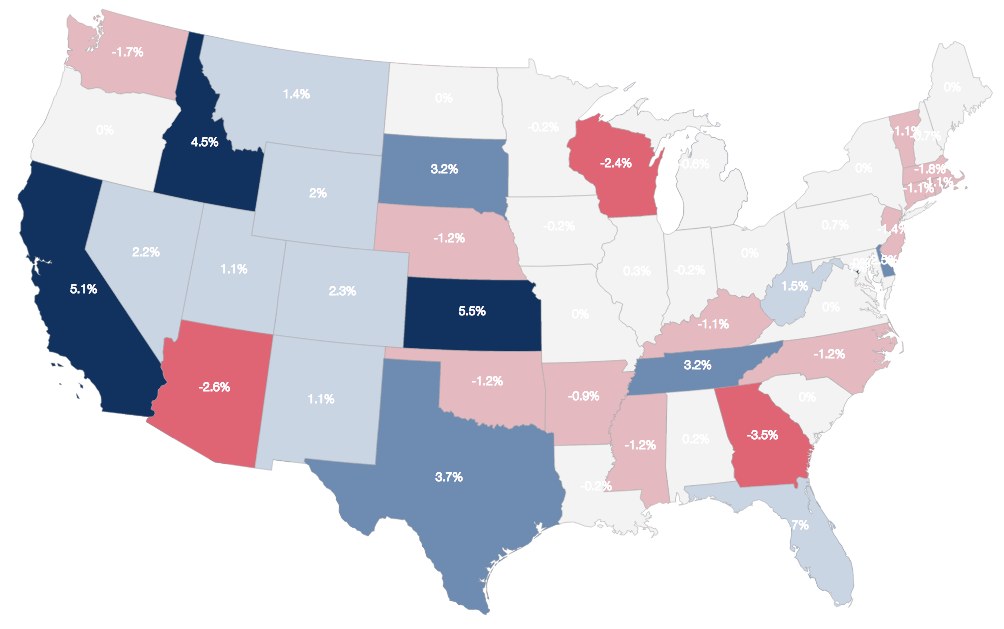
\includegraphics[width=0.8\textwidth]{figures/State_Choropleth.png}
%     \caption
%     [
%         A choropleth map.
%     ]
%     {
%         A choropleth map; \ccLogo~Deepthiyathiender, Wikimedia Commons (2015).
%     }
%     \label{typology:fig:chropleth}
% \end{figure}

According to Munzner's nested model\index{nested model (Munzner)} for visualization design and validation~\cite{Munzner2009}, abstract tasks\index{task!task abstraction} are domain- and interface-agnostic operations that people perform.
Disappointingly, there is little agreement as to the appropriate granularity of an abstract task\index{task!task abstraction} among the many existing classifications in the visualization, \ac{HCI}\index{human-computer interaction (HCI)}, cartography\index{cartography}, and information retrieval\index{information retrieval} literature~\cite{Amar2005,Amar2004,Andrienko2006,Buja1996,Card1999,Casner1991,Chi1998,Chuah1996,Dix1998,Gotz2008,Heer2012,Keim2002,Klein2006,Lee2006,Liu2010,Mullins1993,Pike2009,Pirolli2005,Raskin2000,Roth2012,Roth2013,Roth1990,Shneiderman1996,Spence2007,Springmeyer1992,Tweedie1997,Valiati2006,Ward2004,Wehrend1990,Yi2007,Zhou1998}.
One of the more frequently cited of these~\cite{Amar2005} would classify the above example as being a series of value retrieval tasks\index{task}.
This low-level\index{task!low-level tasks} characterization does not describe the person's context or motivation; nor does take into account prior experience and background knowledge.
For instance, a description of this task\index{task} might differ if the person was unfamiliar with American geography: the person must locate\index{{\tt locate}} and identify\index{{\tt identify}} these states before comparing\index{{\tt compare}} their values.
Conversely, high-level\index{task!high-level tasks} descriptions of exploratory data analysis and presentation emanating from the sensemaking\index{sensemaking} literature~\cite{Amar2004,Card1999,Klein2006,Pirolli2005} cannot aptly describe this person's task\index{task}.

The gap between low-level\index{task!low-level tasks} and high-level\index{task!high-level tasks} classification leaves us unable to abstractly describe tasks\index{task} in a useful way, even for the simple static choropleth map\index{visual encoding!map!choropleth map} in the above example.
This gap widens when interactive visualization techniques are considered, and the complexity of its usage is compounded over time.
We must move beyond describing a single task\index{task} in isolation, to a description that designates when one task\index{task} ends\index{task!ends} and another begins.
To close this gap, visualization tasks\index{task} must be describable in an abstract way across multiple levels.

The primary contribution of this chapter is a multi-level typology\index{task!task typology} of abstract visualization tasks\index{task} that unites the previously disconnected scopes of low-level\index{task!low-level tasks} and high-level\index{task!high-level tasks} classifications by proposing multiple levels of linkage between them.
Our typology\index{task!task typology} provides a powerful and flexible way to describe complex tasks\index{task} as a sequence of interdependent simpler ones\index{task!task sequence}.
While this typology\index{task!task typology} is very much informed by previous work, it is also the result of new thinking and has many points of divergence with existing models.
Central to the organization of our typology\index{task!task typology} are three questions that serve to disambiguate the means\index{task!means} and ends\index{task!ends} of a task\index{task}: {\it why}\index{{\tt why}} data is being visualized, {\it how}\index{{\tt how}} the visualization technique or tool supports the task\index{task}, and {\it what}\index{{\tt what}} are the task's\index{task} inputs\index{{\tt input}} and outputs\index{{\tt output}}.
We have found that no prior characterization of tasks\index{task} satisfactorily answers all of these questions simultaneously at multiple levels of abstraction\index{task!task abstraction}.
Typically, low-level\index{task!low-level tasks} classifications provide a sense of {\it how}\index{{\tt how}} a task\index{task} is performed, but not {\it why}\index{{\tt why}}; high-level\index{task!high-level tasks} classifications are the converse.
One major advantage of our typology\index{task!task typology} over prior work is in providing linkage between these two questions.
Another advantage is the ability to link sequences of tasks\index{task!task sequence}, made possible by the consideration of {\it what}\index{{\tt what}} tasks\index{task} operate on.

Our typology\index{task!task typology} provides a consistent lexicon for description that supports making precise comparisons of tasks\index{task} between different visualization tools and across application domains.
Succinct and abstract descriptions of tasks\index{task} are crucial for analysis of people using visualization tools and techniques.
This analysis is an essential precursor to the effective design and evaluation\index{evaluation} of visualization tools, particularly in the context of problem-driven design studies~\cite{Sedlmair2012}.
In these studies, visualization practitioners work with people from specific application domains to determine {\it why}\index{{\tt why}} and {\it what}\index{{\tt what}}, subsequently drawing from their specialized knowledge of visual encoding\index{visual encoding} and interaction\index{interaction} design choices as well as known human capabilities with respect to perception\index{perception}~\cite{Cleveland1984,Rensink2014} and interaction\index{interaction} to envision {\it how}\index{{\tt how}} that task\index{task} is to be supported.
A need for task analysis\index{task!task analysis} also arises in visualization evaluation~\cite{Lam2012}\index{evaluation}, particularly in observational studies of people using visualization tools and techniques.
Our typology\index{task!task typology} provides a code set for qualitatively describing the behaviour of participants in such studies.

% In \autoref{typology:typology}, we introduce our multi-level typology of abstract visualization tasks.
% In \autoref{typology:results}, we demonstrate the benefits of our approach with a detailed example, in which we describe a sequence of interdependent tasks.
% In \autoref{typology:rw}, we summarize our typology's connections to related work and to its theoretical foundations.
% In \autoref{typology:discussion}, we discuss the value and usage of this typology, as well as our plans for its further validation and extension.

%-------------------------------------------------------------------------
%-------------------------------------------------------------------------

\section{Background Context}
\label{typology:context}

%-------------------------------------------------------------------------
%-------------------------------------------------------------------------

As we expect some readers to be unfamiliar with the context that motivated this work, we begin with a brief discussion of our current inability to succinctly describe and analyze visualization tasks\index{task!task analysis}.
The primary limiting factor in using existing classifications as tools for analysis is that we cannot easily distinguish between the ends\index{task!ends} and means\index{task!means} of tasks\index{task}.
Making this distinction is a central problem for practitioners during the {\it abstraction} phase of design studies~\cite{Sedlmair2012}\index{design studies} and during the analysis phase of qualitative studies of people using visualization tools or techniques~\cite{Lam2012}.

For instance, a number of existing classifications mention the word {\it derive}\index{{\tt derive}}~\cite{Amar2005,Chuah1996,Heer2012,Lee2006,Pike2009,Springmeyer1992}.
Is {\it derive}\index{{\tt derive}} a task\index{task}, or the means\index{task!means} by which another task\index{task} is performed?
A person may derive\index{{\tt derive}} data items as an end in itself, for example to reduce the number of dimensions in a dataset, or as a means\index{task!means} towards another end, such as to verify\index{{\tt discover}} a hypothesis regarding the existence of clusters in a derived low-dimensional space.
The ends-means\index{task!ends}\index{task!means} ambiguity exists for many terms found in existing classifications: consider {\it filter}~\cite{Amar2005,Card1999,Gotz2008,Heer2012,Keim2002,Klein2006,Lee2006,Mullins1993,Pike2009,Pirolli2005,Roth2012,Roth2013,Shneiderman1996,Yi2007}\index{{\tt filter}}, {\it navigate}\index{{\tt navigate}}~\cite{Heer2012,Spence2007,Ward2004}, or {\it record}~\cite{Heer2012,Mullins1993,Springmeyer1992}\index{{\tt record}}.
The first step towards distinguishing ends\index{task!ends} from means\index{task!means} involves asking {\it why}\index{{\tt why}} someone would visualize data separately from {\it how}\index{{\tt how}} the visualization tool or technique supports the task\index{task}, a question that is central to the organization of our typology\index{task!task typology}.

The separation of {\it why}\index{{\tt why}} and {\it how}\index{{\tt how}} does not in itself resolve all confusion.
Consider {\it sort}, another term appearing in existing classifications~\cite{Amar2005,Gotz2008,Heer2012,Lee2006,Pike2009}.
Sorting has an input\index{{\tt input}} and an output\index{{\tt output}}; in some cases, it is items of data within a single view~\cite{Rao1994}; in others, views themselves may be sorted~\cite{Becker1996}\index{view coordination}.
In both cases, the sorted output\index{{\tt output}} can serve as input\index{{\tt input}} to subsequent tasks\index{task}.
The next step in distinguishing ends\index{task!ends} from means\index{task!means} is thus characterizing {\it what}\index{{\tt what}} the task's\index{task} inputs\index{{\tt input}} and outputs\index{{\tt output}} are, allowing us to describe sequences of interdependent tasks\index{task!task sequence}.

To illustrate how the ends-means\index{task!ends}\index{task!means} ambiguity arises during the course of analysis, we will now attempt to use representative existing classification to describe two example tasks\index{task}:

\bstart{Example \#1} recall the example stated above in \autoref{typology:intro}, that of a casual encounter with an electoral map\index{visual encoding!map!choropleth map} in which a person compares\index{{\tt compare}} two regions; election results for each state are encoded\index{{\tt encode}} as a choropleth map\index{visual encoding!map!choropleth map} based on two attributes, candidate and margin of victory.
Furthermore, we know that this person is familiar with American geography and its regions; this prior knowledge dictates the type of search\index{{\tt search}}.

Using the typology\index{task!task typology} of \citet{Andrienko2006}, we might describe this example as an {\it elementary direct comparison task}\index{{\tt compare}}.
While richer than a series of {\it retrieve value} tasks~\cite{Amar2005}, this description tells us little about {\it why}\index{{\tt why}} and {\it how}\index{{\tt how}} this comparison was performed.
Low-level\index{task!low-level tasks} descriptions derived from a number of other classifications  are similarly impoverished~\cite{Casner1991,Gotz2008,Roth1990,Valiati2006,Wehrend1990,Yi2007,Zhou1998}.

We might enrich our description of this task\index{task} using a recent {\it taxonomy of cartographic interaction primitives}\index{cartography} by \citet{Roth2012,Roth2013}, a much more comprehensive approach that distinguishes between {\it goals}, {\it objectives}, {\it operators}, and {\it operands}.
Using his taxonomy, this task\index{task} would be described as follows:

\begin{itemize}
    \item {\bf goals}: {\it procure}
    \item {\bf objectives}: {\it compare}
    \item {\bf operators}: {\it retrieve} and {\it calculate}
    \item {\bf operands}: {\it attribute--in--space} (search target); {\it general} (search level)
\end{itemize}

While the dimensions of this description are similar to the questions of {\it why}\index{{\tt why}}, {\it how}\index{{\tt how}}, and {\it what}\index{{\tt what}}, the description is incomplete, particularly in its classification of {\it goals} and {\it objectives}.
Roth's taxonomy provides us only with a partial sense of {\it how}\index{{\tt how}} the comparison\index{{\tt compare}} is performed: {\it retrieve} does not tells us about whether the person knows the spatial location of the regions to be compared a priori.
The goal, {\it procure}, does not provide us with any higher-level context\index{task!high-level tasks} or motivation for {\it why}\index{{\tt why}} the person is {\it procuring}; specifically, the person's casual interest in these two regions is lost.
Finally, Roth's taxonomy imposes a spatial constraint on {\it operands}, leaving us unable to fully articulate {\it what}\index{{\tt what}} is being compared.

\bstart{Example \#2} in evaluation studies~\cite{Lam2012}\index{evaluation}, it is sometimes necessary to perform a comparative analysis of a task\index{task} being performed using different visualization tools or techniques.
Consider a person using a tree visualization\index{visual encoding!tree} tool whose interest relates to two nodes in a large tree\index{visual encoding!tree}, and her intent is to present the path between these nodes to her colleagues.
SpaceTree~\cite{Grosjean2002} and TreeJuxtaposer~\cite{Munzner2003} are two tree visualization\index{visual encoding!tree} tools that allow people to locate\index{{\tt locate}} paths between nodes by means\index{task!means} of different focus + context\index{view coordination!focus + context} techniques.
Both tools allow for path selection\index{{\tt select}}, in which the encoding of selected paths differs from that of non-selected paths.
The tools differ in {\it how}\index{{\tt how}} the elements that have been visualized are manipulated\index{{\tt manipulate}}:
TreeJuxtaposer allows a person to arrange\index{{\tt arrange}} areas of the tree\index{visual encoding!tree} to ensure visibility for areas of interest, while SpaceTree couples the act of selection\index{{\tt select}} by aggregating\index{{\tt aggregate}} and filtering\index{{\tt filter}} unselected items.

As in the previous example, task\index{task} descriptions from existing classifications seldom answer all three questions: {\it why}\index{{\tt why}}, {\it how}\index{{\tt how}}, and {\it what}\index{{\tt what}}.
Using the {\it taxonomy of interactive dynamics for visual analysis} by \citet{Heer2012}, we might describe this task\index{task} as being an instance of {\it data and view specification} ({\it visualize} and {\it filter}\index{{\tt filter}}) as well as
{\it view manipulation}\index{{\tt manipulate}} ({\it navigate}\index{{\tt navigate}} and {\it select}\index{{\tt select}})\index{view coordination}.
This description tells us {\it how}\index{{\tt how}}, but it doesn't specify {\it why}\index{{\tt why}} the data is being visualized.

We might complement Heer and Shneiderman's description with one based on a taxonomy of graph visualization tasks\index{task} by \citet{Lee2006}, in which this task\index{task} would be classified as a {\it topology task}, namely one of {\it determining connectivity} and subsequently {\it finding the shortest path}.
As the scope of Lee \etal's taxonomy is specialized, we are provided with a clear indication of {\it what}\index{{\tt what}} the person's interest is, this being a {\it path}.
Unfortunately, this description provides only a partial account of {\it why}\index{{\tt why}} data is being visualized; we are not provided with a high-level\index{task!high-level tasks} motivation beyond {\it determining} and {\it finding}.

Both descriptions do not relate the person's actions to the high-level\index{task!high-level tasks} goal of {\it presenting} information to others.
Second, and more importantly, these descriptions fail to distinguish {\it how}\index{{\tt how}} this task\index{task} is performed using SpaceTree from {\it how}\index{{\tt how}} it is performed using TreeJuxtaposer.

\bstart{Summary} these examples demonstrate our inability to comprehensively analyze tasks\index{task!task analysis} using existing classifications of behaviour of people who use visualization tools or techniques.
Note that we are not directly criticizing these classifications; we acknowledge that their scope is often deliberately constrained, with some focusing on low-level tasks\index{task!low-level tasks}, interactions\index{interaction}, or operations~\cite{Amar2005,Andrienko2006,Buja1996,Casner1991,Chi1998,Chuah1996,Dix1998,Gotz2008,Keim2002,Lee2006,Roth1990,Shneiderman1996,Tweedie1997,Valiati2006,Ward2004,Wehrend1990,Yi2007,Zhou1998}, while others focus on high-level tasks\index{task!high-level tasks} or goals~\cite{Amar2004,Card1999,Klein2006,Liu2010,Pirolli2005}, or on the behaviour of people who work in specific domains or contexts~\cite{Lee2006,Roth2012,Roth2013,Sprague2012}.
We lack guidance on how to integrate these disjoint bodies of work, to compose task\index{task} descriptions that draw from all of them.
This integration is the aim of our typology\index{task!task typology}, which will allow practitioners to describe tasks\index{task} that address critical questions posed during visualization design and evaluation\index{evaluation}, namely {\it why}\index{{\tt why}}, {\it how}\index{{\tt how}}, and {\it what}\index{{\tt what}}.

It could be argued that a classification of {\it tasks}\index{task} should focus solely on the goal of the person who uses the visualization tool or technique, or {\it why}\index{{\tt why}} data is visualized; people are often not immediately concerned with {\it how}\index{{\tt how}} a task\index{task} is performed, as long as their task\index{task} can be accomplished.
We argue that by classifying tasks\index{task} according to {\it how}\index{{\tt how}} they are performed, {\it in addition} to {\it why}\index{{\tt why}} they are performed and {\it what}\index{{\tt what}} they pertain to, we can improve communication between visualization practitioners working in different domains, facilitating tool-independent comparisons, the analysis of diverging usage strategies for executing tasks~\cite{Vicente1999,Ziemkiewicz2012}\index{task}, and improved reasoning about design alternatives.

%-------------------------------------------------------------------------
%-------------------------------------------------------------------------

\section{A Typology of Tasks}
\label{typology:typology}

%-------------------------------------------------------------------------
%-------------------------------------------------------------------------

%-|-|-|-|-|-|-|-|-|-|-|-|-|-|-|-|-|-|-|-|-|-|-|-|-|-|-|-|-|-|-|-|-|-|-|-|-


\begin{figure}
    \centering
    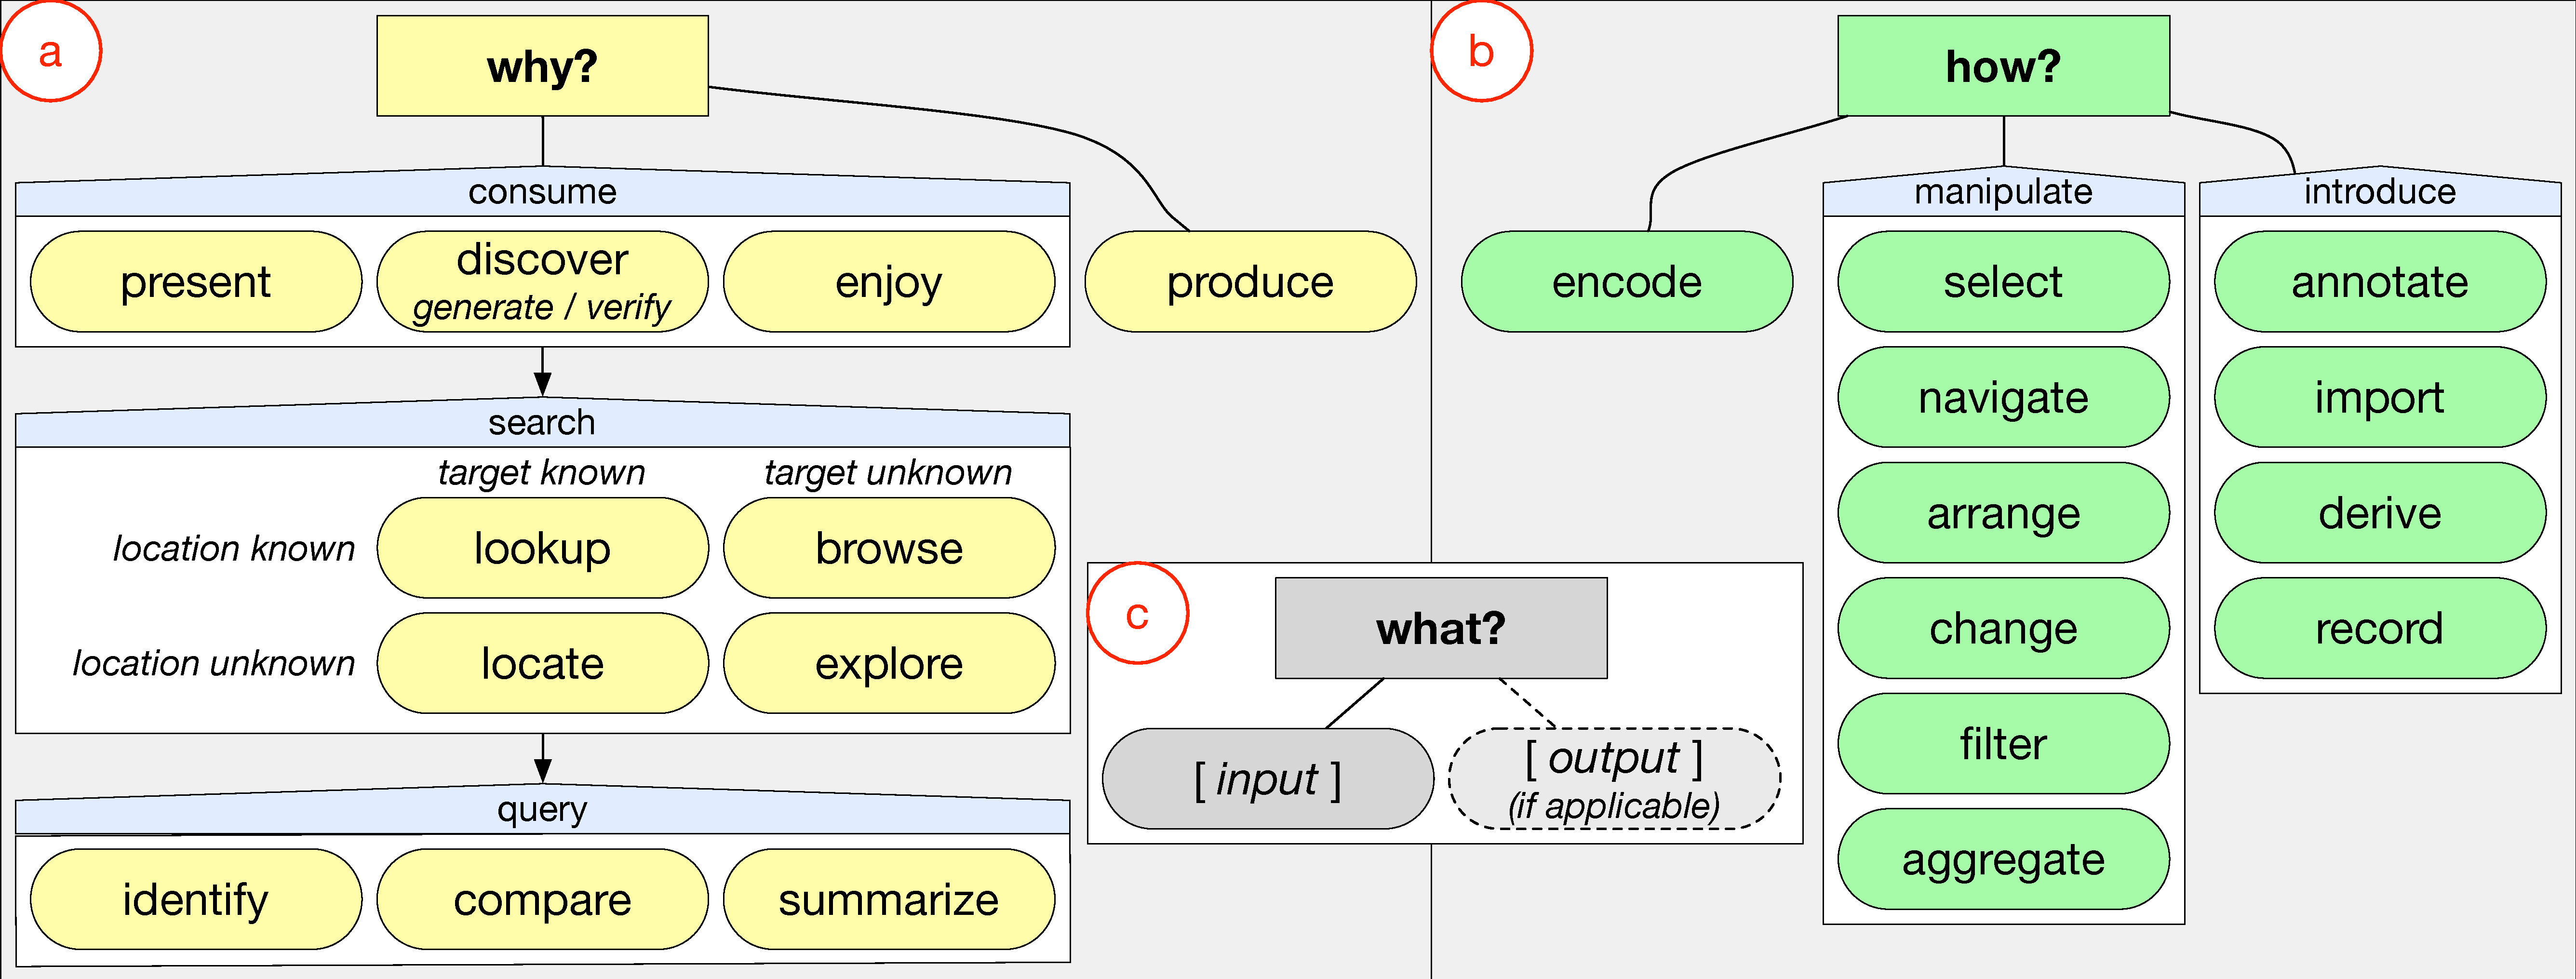
\includegraphics[width=\textwidth]{figures/typology.pdf}
    \caption
    [
        Our multi-level typology of abstract visualization tasks: \textsl{why}, \textsl{how}, and \textsl{what}.
    ]
    {
        Our multi-level typology of abstract visualization tasks.
        The typology spans \textsl{why}, \textsl{how}, and \textsl{what}; task descriptions are formed by nodes from each part:
        (a) \textsl{why} data is visualized, from high-level ({\tt consume} vs.~{\tt produce}) to mid-level ({\tt search}) to low-level ({\tt query});
        (b) \textsl{how} a visualization tool or technique supports the task in terms of visual encoding and interaction design choices;
        (c) \textsl{what} the task {\tt inputs} and {\tt outputs} are.
    }
    \label{typology:fig:typology}
\end{figure}

%-|-|-|-|-|-|-|-|-|-|-|-|-|-|-|-|-|-|-|-|-|-|-|-|-|-|-|-|-|-|-|-|-|-|-|-|-


Our multi-level typology\footnote{We denote this work as a {\it typology}, rather than a {\it taxonomy}, as the former is appropriate for classifying abstract concepts, while the latter is appropriate for classifying empirically observable events~\cite{Bailey1994}. For instance, one could construct a taxonomy of the observable ways in which a person could interact with a particular visualization tool, or a taxonomy of existing visual encoding\index{visual encoding} design choices for tree-based data~\cite{Schulz2011}.}\index{task!task typology} of abstract visualization tasks\index{task!task abstraction}, represented in \autoref{typology:fig:typology}, is encapsulated by three questions: {\it why}\index{{\tt why}} the data is being visualized, {\it how}\index{{\tt how}} the visualization tool or technique supports the task\index{task}, and {\it what}\index{{\tt what}} does the task\index{task} pertain to (\autoref{typology:fig:typology}a-c).
Complete task\index{task} descriptions, such as those for Examples \#1-2 (represented in \autoref{typology:fig:task_examples}), must include nodes from all three parts of this typology.
%RR: p.24 "taxonomy" vs "typology". The latter is apparently used for abstract concepts. But wouldn't the higher levels of a taxonomy also be abstract? If so, this distinction would apply just to the leaf nodes. And a set of existing systems would presumably be handled by a "taxonomy", but would then be discussed with reference to a "typology". Is this distinction really all that helpful? Or does it cause more confusion than it's worth?
In the remainder of this dissertation, we use a {\tt fixed-width font} to highlight vocabulary from this typology\index{task!task typology}; this vocabulary is also indexed separately at the end of this dissertation.

This structure, while unusual relative to many existing classifications, mirrors the analytical thinking process undertaken in design studies~\cite{Sedlmair2012}.
{\it Why}\index{{\tt why}}, {\it what}\index{{\tt what}}, and {\it how}\index{{\tt how}} are also used in {\it Cognitive Work Analysis} by \citet{Vicente1999}\index{cognitive work analysis (Vicente)}, particularly for relating abstractions within a work domain\index{work domain analysis}, as well as in an analysis of techniques and tools for visualizing time-oriented data by \citet{Aigner2011}, which asks {\it what is presented?}, {\it why is it presented?}, and {\it how is it presented?}.

We will introduce {\it why}\index{{\tt why}} before {\it how}\index{{\tt how}}, as this order reflects the translation of empirically observable domain problems into abstract tasks\index{task!task abstraction} and subsequently into visual encoding\index{visual encoding} and interaction\index{interaction} design choices: practitioners first determine {\it why}\index{{\tt why}} data is visualized, and then must decide upon {\it how}\index{{\tt how}} the visualization tool or technique will support the task\index{task}.
We then discuss the {\it what}\index{{\tt what}} part of our typology\index{task!task typology}, which considers the {\tt input}\index{{\tt input}} and {\tt output}\index{{\tt output}} of tasks\index{task}.
Our typology\index{task!task typology} supports the description of a complex domain-specific visualization workflow\index{workflows} as a sequence of interdependent tasks\index{task!task sequence}, where the {\tt output}\index{{\tt output}} of a prior task\index{task} may serve as the {\tt input}\index{{\tt input}} to a subsequent task\index{task}, as we demonstrate in the example featured in \autoref{typology:results}.

For clarity, we first present our typology\index{task!task typology} in its entirety with minimal discussion of the previous work that informed its organization, and then focus on these connections in \autoref{typology:rw} and in \autoref{typology:tab:rw:why} and \autoref{typology:tab:rw:how}.

%-------------------------------------------------------------------------

\subsection{Why is Data Being Visualized?}
\label{typology:why}

%-------------------------------------------------------------------------

The {\it why}\index{{\tt why}} part of our typology\index{task!task typology}, shown in \autoref{typology:fig:typology}a, allows us to describe {\it why}\index{{\tt why}} the data is being visualized, and includes multiple levels of abstraction, a narrowing of scope from high-level\index{task!high-level tasks} ({\tt consume} vs. {\tt produce}\index{{\tt produce}}) to mid-level\index{task!mid-level tasks} ({\tt search}\index{{\tt search}}) to low-level\index{task!low-level tasks} ({\tt query}\index{{\tt query}}).

\bstart{Consume}
People visualize data in order to {\tt consume}\index{{\tt consume}} information in many domain contexts.
In most cases, this consumption is driven either by a need to present information or to discover\index{{\tt discover}} and analyze new information~\cite{vanWijk2006}.
However, there are many other contexts in which the information being visualized is simply enjoyed~\cite{Dork2012,Pousman2007,Sprague2012}\index{{\tt enjoy}}, where people indulge their casual interests in a topic.

{\tt Present}\index{{\tt present}}
refers to the visualization of data for the succinct communication of information, for telling a story with data\index{storytelling}, guiding an audience through a series of cognitive operations.
Presentation using a visualization technique or tool may take place within the context of decision making, planning, forecasting, and instructional processes~\cite{Friel2001,Marchionini2006,Roth2012,Roth2013}.
Presentation brings to mind collaborative and pedagogical contexts, and the way in which a presentation is given may vary according to the size of the audience, whether the presentation is live or pre-recorded, and whether the audience is co-located with the presenter~\cite{Kosara2013}.

{\tt Discover}\index{{\tt discover}}
is about the generation and verification of hypotheses and is associated with modes of scientific inquiry~\cite{Pike2009}.
Scientific investigation may be motivated by existing theories, models, and hypotheses, or by the serendipitous observation of unexpected phenomena~\cite{Andre2009}.

{\tt Enjoy}\index{{\tt enjoy}}
refers to casual encounters with visualized data~\cite{Pousman2007,Sprague2012}.
In these contexts, a person is not driven by a need to verify\index{{\tt discover}} or generate\index{{\tt discover}} a hypothesis; novelty stimulates curiosity and thereby exploration~\cite{Dork2011,Sprague2012,Stephenson1967,Toms2000}\index{{\tt explore}}.
This motivation is notably absent from existing classifications, as shown in \autoref{typology:tab:rw:why} and \autoref{typology:tab:rw:how}.
Casual encounters with visualized data can be fleeting, such as in the earlier example of encountering a static choropleth electoral map\index{visual encoding!map!choropleth map} while reading a blog post.
Conversely, these encounters might be immersive and time-consuming experiences, such as in museum settings~\cite{Pousman2007}.

\bstart{Produce}
we use {\tt produce}\index{{\tt produce}} in reference to tasks\index{task} in which the intent is to generate new information.
This information includes but is not limited to: transformed or derived data\index{{\tt derive}}, annotations, recorded interactions\index{{\tt record}}, or screenshots of static visualizations.
Examples of {\tt produce}\index{{\tt produce}} in previous work include the production of graphical annotations and explanatory notes to describe features of line graphs\index{visual encoding!line graph} of time series data\index{time-oriented data}~\cite{Willett2012}, or the production of {\it graphical histories} in Tableau intended to document the analytical provenance\index{analytical provenance} of a person using this tool~\cite{Heer2008}.
Additional examples of {\tt produce}\index{{\tt produce}} involving derived data and annotations\index{{\tt annotate}} are featured in the example of \autoref{typology:results}.

It is important to note that the products of a {\tt produce}\index{{\tt produce}} task\index{task} may be used in some subsequent task\index{task} that may or may not involve a visualization tool or technique.
For example, some visualization tools for analyzing high-dimensional data allow people to {\tt produce}\index{{\tt produce}} new categorical attributes for labelling clustered data points in a dimensionally reduced\index{dimensionality reduction (DR)} coordinate space; these attributes might be used later for constructing a predictive model.

\bstart{Search}
Regardless of whether the intent is to {\tt present}\index{{\tt present}}, {\tt discover}\index{{\tt discover}}, or merely {\tt enjoy}\index{{\tt enjoy}}, a person will {\tt search}\index{{\tt search}} for aspects of interest in the visualized data.
While terms relating to {\tt search}\index{{\tt search}} and exploration\index{{\tt explore}} are often conflated~\cite{Marchionini2006,Toms2000}, we have imposed a characterization of {\tt search}\index{{\tt search}} that depends on {\it what}\index{{\tt what}} is being sought.
We classify them according to whether the identity or location of the search target is known a priori.
Whether the identity of the search target is known recalls the concept of {\it references} and {\it characteristics} introduced by \citet{Andrienko2006}: {\tt searching}\index{{\tt search}} for known reference targets entails {\tt lookup}\index{{\tt lookup}} or {\tt locate}\index{{\tt locate}}, while {\tt searching}\index{{\tt search}} for targets matching particular characteristics entails {\tt browse}\index{{\tt browse}} or {\tt explore}\index{{\tt explore}}.
Consider our earlier example of a person who is familiar with American geography and is {\tt searching}\index{{\tt search}} for California on an choropleth map\index{visual encoding!map!choropleth map}; we would describe this as an instance of {\tt lookup}\index{{\tt lookup}}.
However, a person who is {\it unfamiliar} with American geography must {\tt locate}\index{{\tt locate}} California.

In contrast, the identity of a search target might be unknown a priori; a person may be {\tt searching}\index{{\tt search}} for characteristics rather than references~\cite{Andrienko2006}; these characteristics might include particular values, extremum, anomalies, trends, or  ranges~\cite{Amar2005}.
For instance, if a person using a tree-based visual encoding\index{visual encoding!tree} is {\tt searching}\index{{\tt search}} within a particular subtree for leaf nodes having few siblings, we would describe this as an instance of {\tt browse}\index{{\tt browse}} because the location is known a priori.
Finally, {\tt explore}\index{{\tt explore}} entails {\tt searching}\index{{\tt search}} for characteristics without regard to their location; many visualization tools provide an overview of the data, which is often the starting point for exploration\index{{\tt explore}}.
Examples include {\tt searching}\index{{\tt search}} for outliers in a scatterplot\index{visual encoding!scatterplot}, for anomalous spikes or periodic patterns in a line graph\index{visual encoding!line graph} of time series data\index{time-oriented data}, or for unanticipated spatially-dependent patterns in a choropleth map\index{visual encoding!map!choropleth map}.

\bstart{Query}\index{{\tt query}}
Once a target or set of targets has been found, a person will
{\tt identify}\index{{\tt identify}}, {\tt compare}\index{{\tt compare}}, or {\tt summarize}\index{{\tt summarize}} these targets.
If a search returns known or {\it reference} targets~\cite{Andrienko2006}, either by {\tt lookup}\index{{\tt lookup}} or {\tt locate}\index{{\tt locate}}, {\tt identify}\index{{\tt identify}} returns their {\it characteristics}.
For example, someone who uses a choropleth map\index{visual encoding!map!choropleth map} representing election results can {\tt identify}\index{{\tt identify}} the winning candidate and margin of victory for the state of California.
Conversely, if a search returns targets matching particular {\it characteristics}, either by {\tt browse}\index{{\tt browse}} or {\tt explore}\index{{\tt explore}}, {\tt identify}\index{{\tt identify}} returns {\it references}.
For instance, our election map\index{visual encoding!map!choropleth map} enthusiast can {\tt identify}\index{{\tt identify}} the state having the highest margin of victory.

The progression from {\tt identify}\index{{\tt identify}} to {\tt compare}\index{{\tt compare}} to {\tt summarize}\index{{\tt summarize}} corresponds to an increase in the amount of search targets under consideration~\cite{Andrienko2006,Buja1996,Tweedie1997}, in that {\tt identify}\index{{\tt identify}} refers to a single target, {\tt compare}\index{{\tt compare}} refers to multiple subsets of targets, and {\tt summarize}\index{{\tt summarize}} refers to a whole set of targets.
As with {\tt explore}\index{{\tt explore}}, {\tt summarize}\index{{\tt summarize}} is also often associated with overviews of the data~\cite{Lee2006}.
Continuing with the choropleth map\index{visual encoding!map!choropleth map} example, the person {\tt identifies}\index{{\tt identify}} the election results for one state, {\tt compares}\index{{\tt compare}} the election results of one state to another, or {\tt summarizes}\index{{\tt summarize}} the election results across all states, determining how many favoured one candidate or the other, or the overall distribution of margin of victory values.

%-------------------------------------------------------------------------

\subsection{How Does the Visualization Technique or Tool Support the Task?}
\label{typology:how}

%-------------------------------------------------------------------------


We now turn our consideration to the {\it how}\index{{\tt how}} part of our typology\index{task!task typology}, which contains {\it idioms}, defined as families of related visual encoding\index{visual encoding} and interaction\index{interaction} design choices.
This part of our typology\index{task!task typology}, shown in \autoref{typology:fig:typology}b, is likely to be most familiar to readers, as it contains a number of {\it idioms} associated with interaction\index{interaction} design choices that are well-represented by several existing classifications \cite{Gotz2008,Mullins1993,Roth2012,Roth2013,Yi2007}.
%RR: p, 28 - Are idioms essentially alternate ways of carrying out a process? If so, perhaps compare them with the design templates sometimes proposed for architecture. (Alexander - a pattern language)
We distinguish between three classes of idioms: those for {\tt encoding}\index{{\tt encode}} data, those for {\tt manipulating}\index{{\tt manipulate}} previously encoded elements, and those for {\tt introducing} new elements.

\bstart{Encode}
The majority of visualization tasks\index{task} rely on {\it how}\index{{\tt how}} data is initially encoded\index{{\tt encode}} as a visual representation\footnote{Some tasks do not depend on {\it how} the data is visually encoded, or take place before the data is encoded; consider, for instance, {\tt produce} tasks that involve {\tt deriving} new data or {\tt recording} states of a visual analysis process or presentation for downstream consumption.}.
A full enumeration of visual encoding\index{visual encoding} design choices for various datatypes beyond the scope of this chapter and appears in Munzner's book~\cite{Munzner2014}.

\bstart{Manipulate}\index{{\tt manipulate}} 
The following idioms affect previously encoded\index{{\tt encode}} elements, modifying them to some extent.
These idioms represent families of interrelated design choices incorporating both interaction\index{interaction} and visual encoding\index{visual encoding}.
We consider visual encoding\index{visual encoding} and interaction\index{interaction} design choices in a unified way because many idioms incorporate aspects of both~\cite{Meyer2015,Munzner2009}, such as focus + context\index{view coordination!focus + context} techniques~\cite{Grosjean2002,Munzner2003}.

{\tt Select}\index{{\tt select}}
refers to the demarcation of one or more encoded\index{{\tt encode}} elements, differentiating selected from unselected elements~\cite{Raskin2000}.
Examples range from directly clicking or lassoing elements in a scatterplot\index{visual encoding!scatterplot} to brushing\index{view coordination!brushing across views} design choices used to highlight elements in visualization tools incorporating multiple linked views~\cite{Weaver2007}\index{view coordination}.

{\tt Navigate}\index{{\tt navigate}}
refers to instances where the person using a visualization tool or technique alters their viewpoint, such as zooming, panning, and rotating.
Other navigation instances include the triggering of details-on-demand\index{view coordination!details-on-demand} views, combining {\tt navigate}\index{{\tt navigate}} and {\tt select}\index{{\tt select}}~\cite{Shneiderman1996}.

{\tt Arrange}\index{{\tt arrange}}
refers to the process of organizing encoded\index{{\tt encode}} elements spatially.
This includes arranging representations of data~\cite{Liu2010,Mullins1993,Wilkinson2005}, such as reordering the axes in a parallel coordinates plot\index{visual encoding!parallel coordinates plot} or the rows and columns of a \ac{SPLOM}\index{visual encoding!scatterplot!scatterplot matrix (SPLOM)}.
Other forms of arrangement allow people to coordinate the spatial layout of views~\cite{Heer2012,Weaver2007}\index{view coordination}.

{\tt Change}\index{{\tt change}}
pertains to alterations in visual encoding\index{visual encoding}.
Simple examples include altering the size and transparency of points in a scatterplot\index{visual encoding!scatterplot} or edges in a node-link graph\index{visual encoding!node-link graph}, altering a colour-scale or texture mapping, or transforming the scales of axes.
Other alterations have more pronounced effects, changing the visual encoding\index{visual encoding}, such as transitioning between grouped\index{visual encoding!bar chart!grouped bar chart} and stacked bar charts\index{visual encoding!bar chart!stacked bar chart}, or between linear and radial layouts for line graphs\index{visual encoding!line graph} of time series data\index{time-oriented data}.
Pronounced changes in visual encoding\index{visual encoding} such as these are often facilitated by smoothly animated transitions\index{view coordination!animated transitions}, which reduce their disruptive effects~\cite{Heer2007}.

{\tt Filter}\index{{\tt filter}}
refers to adjustments to the exclusion and inclusion criteria for encoded\index{{\tt encode}} elements.
Some forms of filtering allow for elements to be temporarily hidden from view and later restored, while other forms are synonymous with outright deletion.
As an example of temporary {\tt filtering}\index{{\tt filter}}, consider a person examining an age histogram\index{visual encoding!histogram} based on population census data.
First, she decides to exclude males, then further adjusts her filter criteria to focus solely on unemployed females.
Finally, she revises the gender criteria to focus on unemployed males.

A common example of permanent {\tt filtering}\index{{\tt filter}}, or deletion, is that of manually {\tt selecting}\index{{\tt select}} and removing outliers resulting from errors in data entry.
Alternatively, consider a scatterplot\index{visual encoding!scatterplot} in which some data points are labelled with manually generated categorical tags.
Deleting a tag would remove this categorical label from all data points having that tag.

{\tt Aggregate}\index{{\tt aggregate}}
concerns changes in the granularity of encoded\index{{\tt encode}} elements; we also consider its converse, segregate, as being associated with this family of design choices.
For example, a person may adjust the granularity of a continuous time scale in a line graph\index{visual encoding!line graph}, aggregating daily values into monthly values, or segregating annual values into quarterly values.
Alternatively, a person may aggregate a clique within a node-link graph\index{visual encoding!node-link graph} into a representative glyph, or segregate clique glyphs into their component nodes.

\bstart{Introduce}
While {\tt manipulate}\index{{\tt manipulate}} idioms alter previously encoded\index{{\tt encode}} elements, {\tt introduce} idioms add new elements.

{\tt Annotate}\index{{\tt annotate}}
refers to the addition of graphical or textual annotations associated with one or more encoded\index{{\tt encode}} elements.
When an annotation is associated with data elements, an annotation could be thought of as a new attribute for these elements.
The earlier example of manually tagging points in a scatterplot\index{visual encoding!scatterplot} with categorical labels is one such instance of annotating data.

{\tt Import}\index{{\tt import}}
pertains to the addition of new data elements.
In some environments, these new data elements might be loaded from external sources, while others might be manually generated.

{\tt Derive}\index{{\tt derive}}
refers to the computation of new data elements given existing data elements.
Aggregating\index{{\tt aggregate}} data often implies deriving data, however this may not always be true: we further specify that derived data must be persistent, while aggregated data need not be.
For instance, a person might {\tt derive} new attributes for tabular data using a \ac{MDS}\index{dimensionality reduction (DR)!multi-dimensional scaling (MDS)} algorithm.

Finally, {\tt record}\index{{\tt record}}
refers to the saving or capturing of elements as persistent artefacts.
As a consequence, {\tt record}\index{{\tt record}} is often associated with {\tt produce}\index{{\tt produce}}.
These artefacts include screen shots, annotations, lists of bookmarked elements or locations, parameter settings, or interaction logs~\cite{Shrinivasan2008}\index{interaction!interaction logs}.
An interesting example of {\tt record}\index{{\tt record}} is that of assembling a {\it graphical history}~\cite{Heer2008}, in which the {\tt output}\index{{\tt output}} of each task\index{task} includes a static snapshot of the state of the visualization tool, and as these snapshots accumulate they are encoded\index{{\tt encode}} as a branching tree\index{visual encoding!tree}.
{\tt Recording}\index{{\tt record}} and retaining artefacts such as these are often desirable for maintaining a sense of analytical provenance\index{analytical provenance}, allowing people who use the tool to revisit earlier states or parameter settings.

%-------------------------------------------------------------------------

\subsection{What are the Inputs and Outputs of the Task?}
\label{typology:what}

%-------------------------------------------------------------------------

Previous work has reached no agreement on the question of {\it what}\index{{\tt what}} is visualized.
Many classifications do not address it at all; others discuss {\it what}\index{{\tt what}} implicitly, as indicated by the parenthetical terms in \autoref{typology:tab:rw:why} and \autoref{typology:tab:rw:how}.
Of those that classify {\it what}\index{{\tt what}}, some focus on the level of the entire dataset, such as {\it tables} composed of {\it values} and {\it attributes} or {\it networks} composed of {\it nodes} and {\it links}~\cite{Shneiderman1996}.
Others allow more precise specification of data-attribute semantics, such as {\it categorical}, {\it ordinal}, and {\it quantitative}~\cite{Card1999}.
A few classifications include not only {\it data} but also {\it views} as first-class citizens~\cite{Chi1998,Chuah1996,Heer2012,Ward2004}\index{view coordination}.
Specific examples of {\it what}\index{{\tt what}} as classified in previous work include: 

\begin{itemize}

    \item Values, extremum, ranges, distributions, anomalies, clusters, correlations~\cite{Amar2005}.
    
    \item {\it Graph-specific objects}~\cite{Lee2006}: nodes, links, paths, graphs, connected components, clusters, groups.
    
    \item {\it Time-oriented primitives}~\cite{Aigner2011}: points, intervals, spans, temporal patterns, rates of change, sequences, synchronization.
    
    \item {\it Interaction operands}~\cite{Ward2004}: pixels, data [values, structures], attributes, geometric [objects, surfaces], visualization structures.
    
\end{itemize}

%-|-|-|-|-|-|-|-|-|-|-|-|-|-|-|-|-|-|-|-|-|-|-|-|-|-|-|-|-|-|-|-|-|-|-|-|-

In this typology\index{task!task typology}, we have chosen a flexible and agnostic representation of {\it what}\index{{\tt what}} that accommodates all of these modes of thinking: in short, we have a ``bring your own {\it what}\index{{\tt what}}'' mentality.
The only absolute requirement is to explicitly distinguish a task's\index{task} {\tt input}\index{{\tt input}} and {\tt output}\index{{\tt output}} constraints when describing sequences of interdependent tasks~\cite{Tweedie1997}\index{task!task sequence}.
An extensive discussion of {\it what}\index{{\tt what}} that dovetails well with this typology\index{task!task typology} appears in Munzner's book~\cite{Munzner2014}\footnote{\citet{Munzner2014} provides a structured classification of data as well as a classification of {\it targets}; both can be used in the analysis of {\tt inputs} and {\tt outputs}. 
The classification of {\it targets} is represented in \autoref{fig:typology-targets}.}. %, but it cannot be effectively summarized in a few paragraphs; thus, it is beyond the scope of this chapter.
% RR: p. 32. - "[what] cannot be effectively summarized in a few paragraphs." Really? This is a very Wittgensteinian remark. What makes you believe that it cannot be summarized? Things that cannot be compressed are usually regarded as random noise. Is there no central point?


%-------------------------------------------------------------------------

\subsection{Concise Task Descriptions}
\label{typology:task descriptions}

%-------------------------------------------------------------------------

Our multi-level typology\index{task!task typology} can be used to concisely describe visualization tasks\index{task}.
Each task\index{task} is defined by {\it why}\index{{\tt why}} data is being visualized, {\it how}\index{{\tt how}} the visualization tool or technique supports the task\index{task}, and by {\it what}\index{{\tt what}} are the {\tt inputs}\index{{\tt input}} and {\tt outputs}\index{{\tt output}} of the task\index{task}.
Single tasks\index{task} may involve multiple nodes from each part of the typology\index{task!task typology}, as shown in \autoref{typology:fig:task_examples}.

%-|-|-|-|-|-|-|-|-|-|-|-|-|-|-|-|-|-|-|-|-|-|-|-|-|-|-|-|-|-|-|-|-|-|-|-|-

\begin{figure}
    \centering
    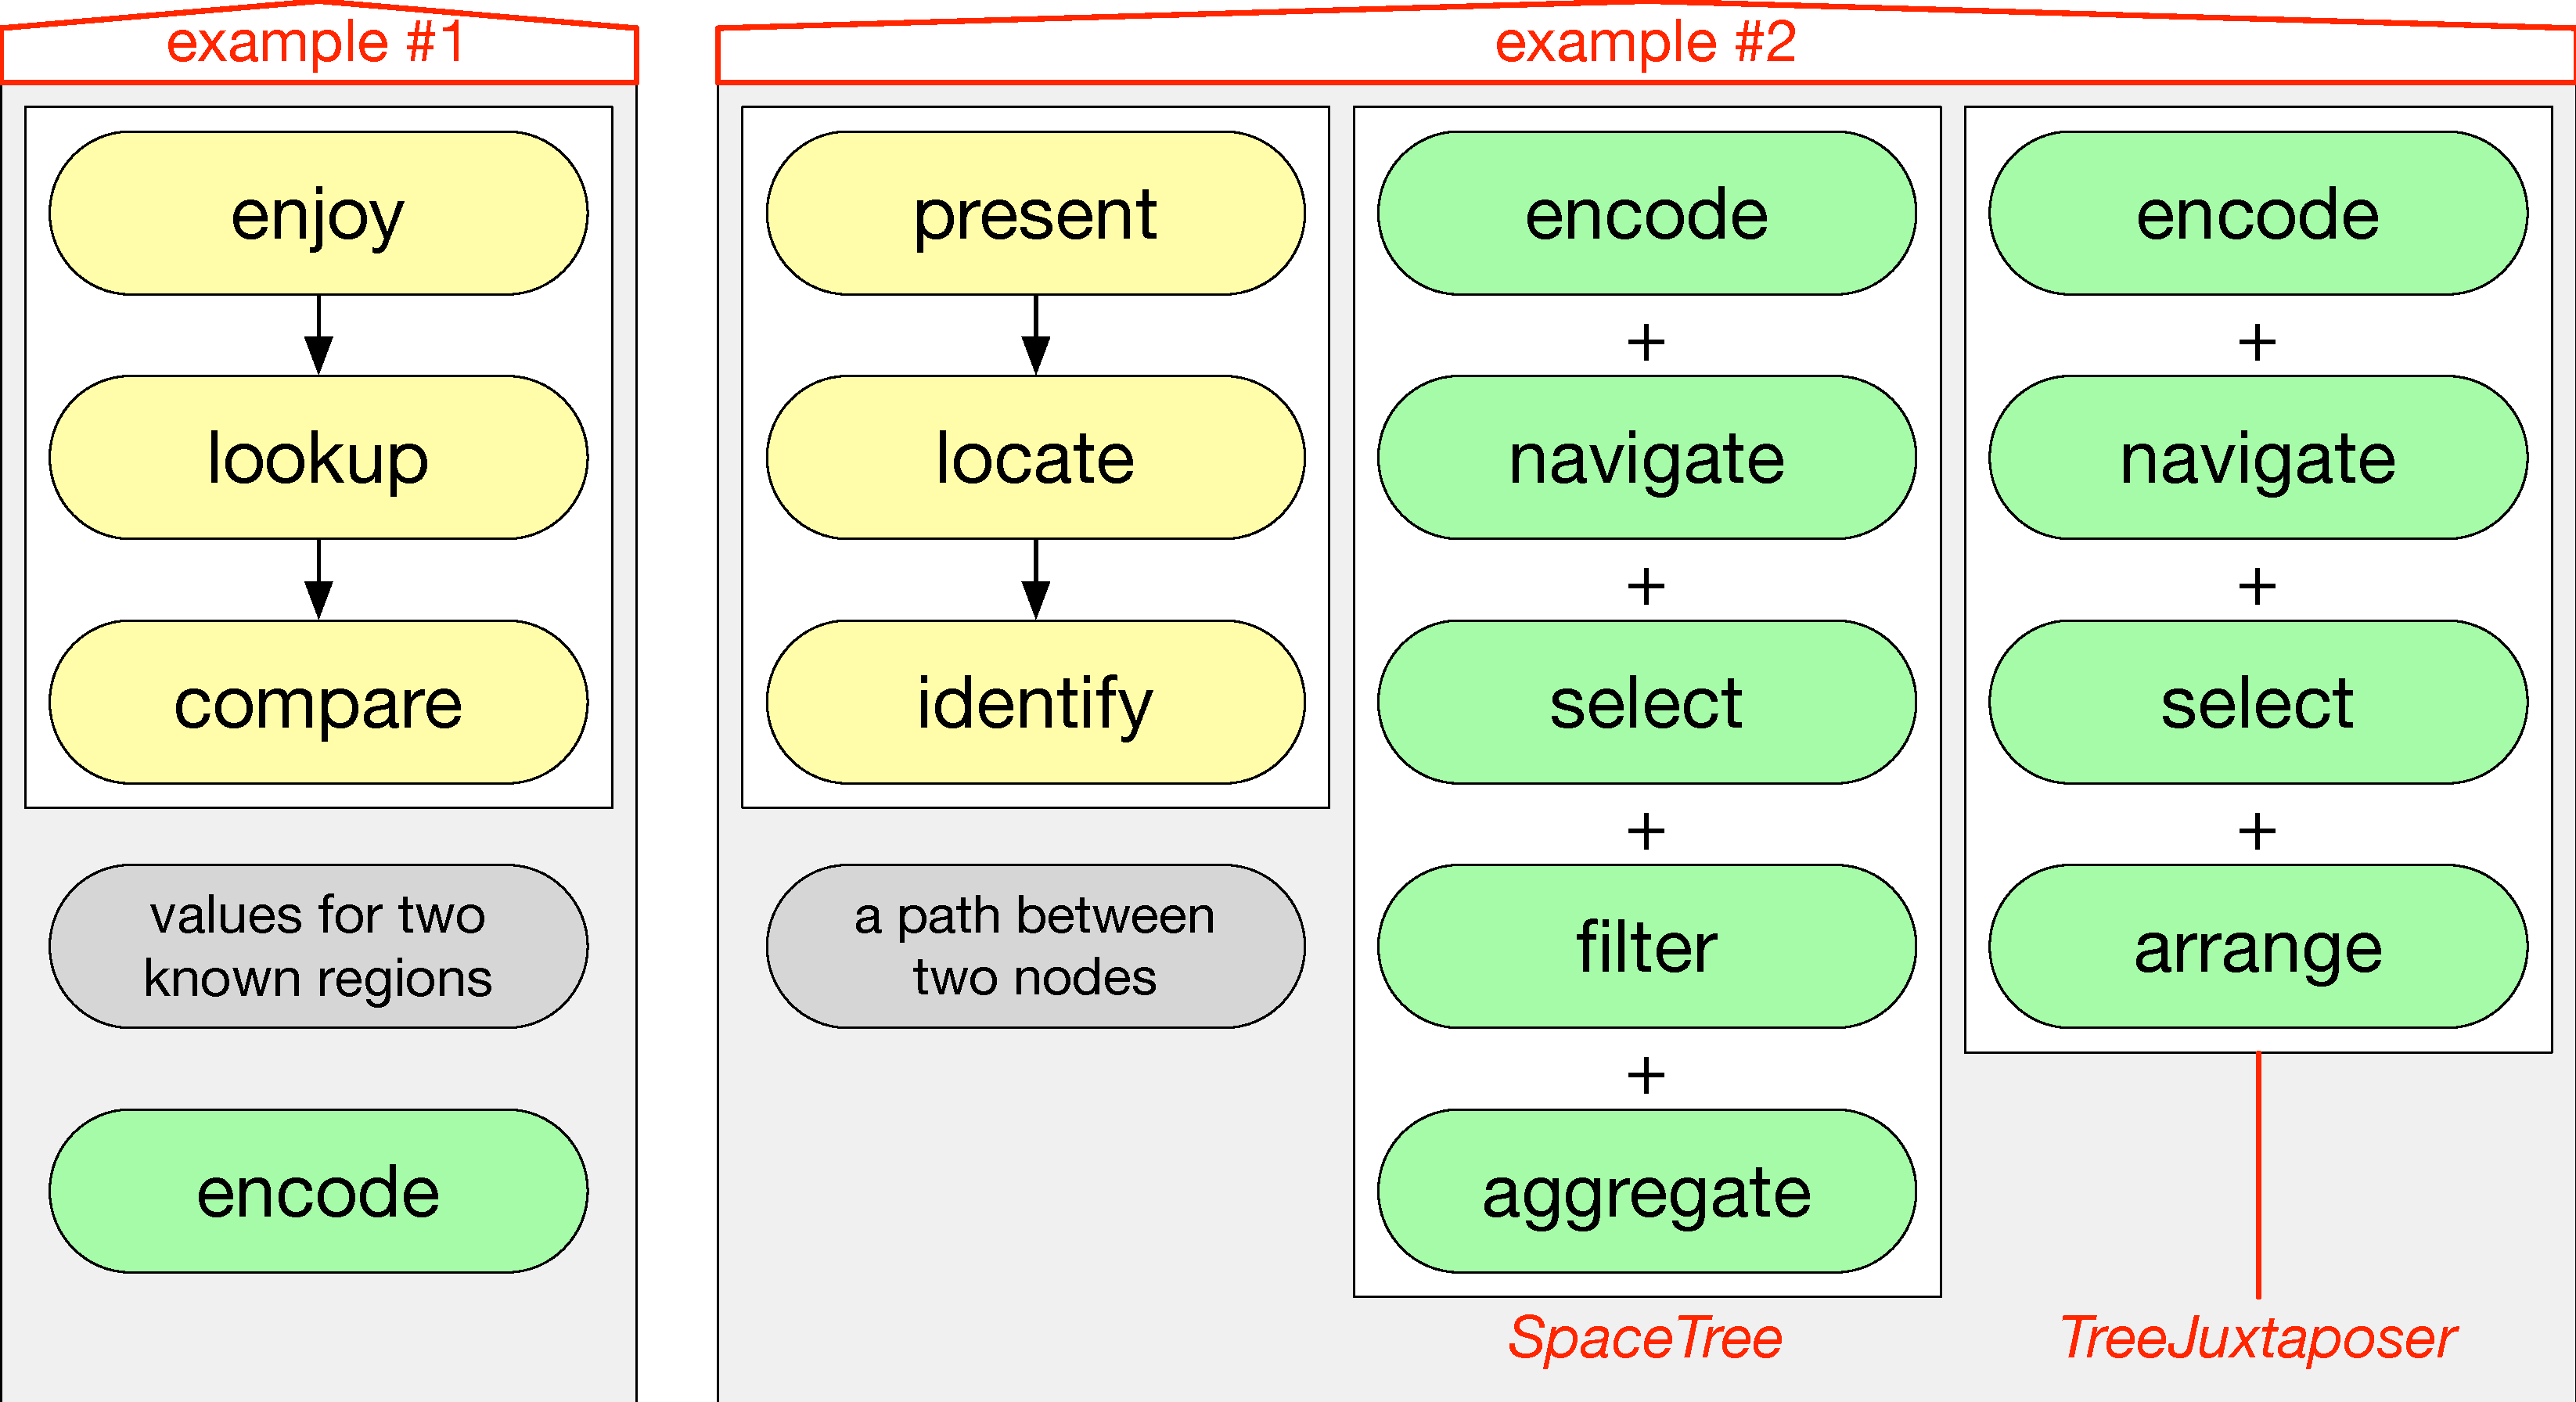
\includegraphics[width=\textwidth]{figures/task_examples.pdf}
    \caption
    [
        Task descriptions for Example \#1 (choropleth map) and Example \#2 (large trees).
    ]
    {
        Task descriptions for Example \#1 (left): casually encountering an choropleth electoral map and comparing election results for two regions; and Example \#2 (right): presenting a path between two nodes in a large tree using SpaceTree~\cite{Grosjean2002} and TreeJuxtaposer~\cite{Munzner2003}.
    }
    \label{typology:fig:task_examples}
\end{figure}

%-|-|-|-|-|-|-|-|-|-|-|-|-|-|-|-|-|-|-|-|-|-|-|-|-|-|-|-|-|-|-|-|-|-|-|-|-

We have chosen to present these descriptions using a simple and flexible visual notation, rather than with a formal grammar~\cite{Andrienko2006,Lammarsch2012,Schulz2013,Tweedie1997,Wilkinson2005}; in doing so, creating and iterating on task\index{task} descriptions can be easily integrated into existing collaborative design and ideation activities, making use of materials such as coloured sticky notes and whiteboards.
A crucial aspect of these descriptions is that sequences of interdependent tasks\index{task} can be chained together\index{task!task sequence}, such that the {\tt output}\index{{\tt output}} from earlier tasks\index{task} forms the {\tt input}\index{{\tt input}} to later tasks\index{task}, as discussed in the following example and as represented in \autoref{typology:fig:task_chain}.

%-------------------------------------------------------------------------
%-------------------------------------------------------------------------

\section{Example: A Sequence of Interdependent Tasks}
\label{typology:results}

%-------------------------------------------------------------------------
%-------------------------------------------------------------------------

%-|-|-|-|-|-|-|-|-|-|-|-|-|-|-|-|-|-|-|-|-|-|-|-|-|-|-|-|-|-|-|-|-|-|-|-|-

\begin{figure}
    \centering
    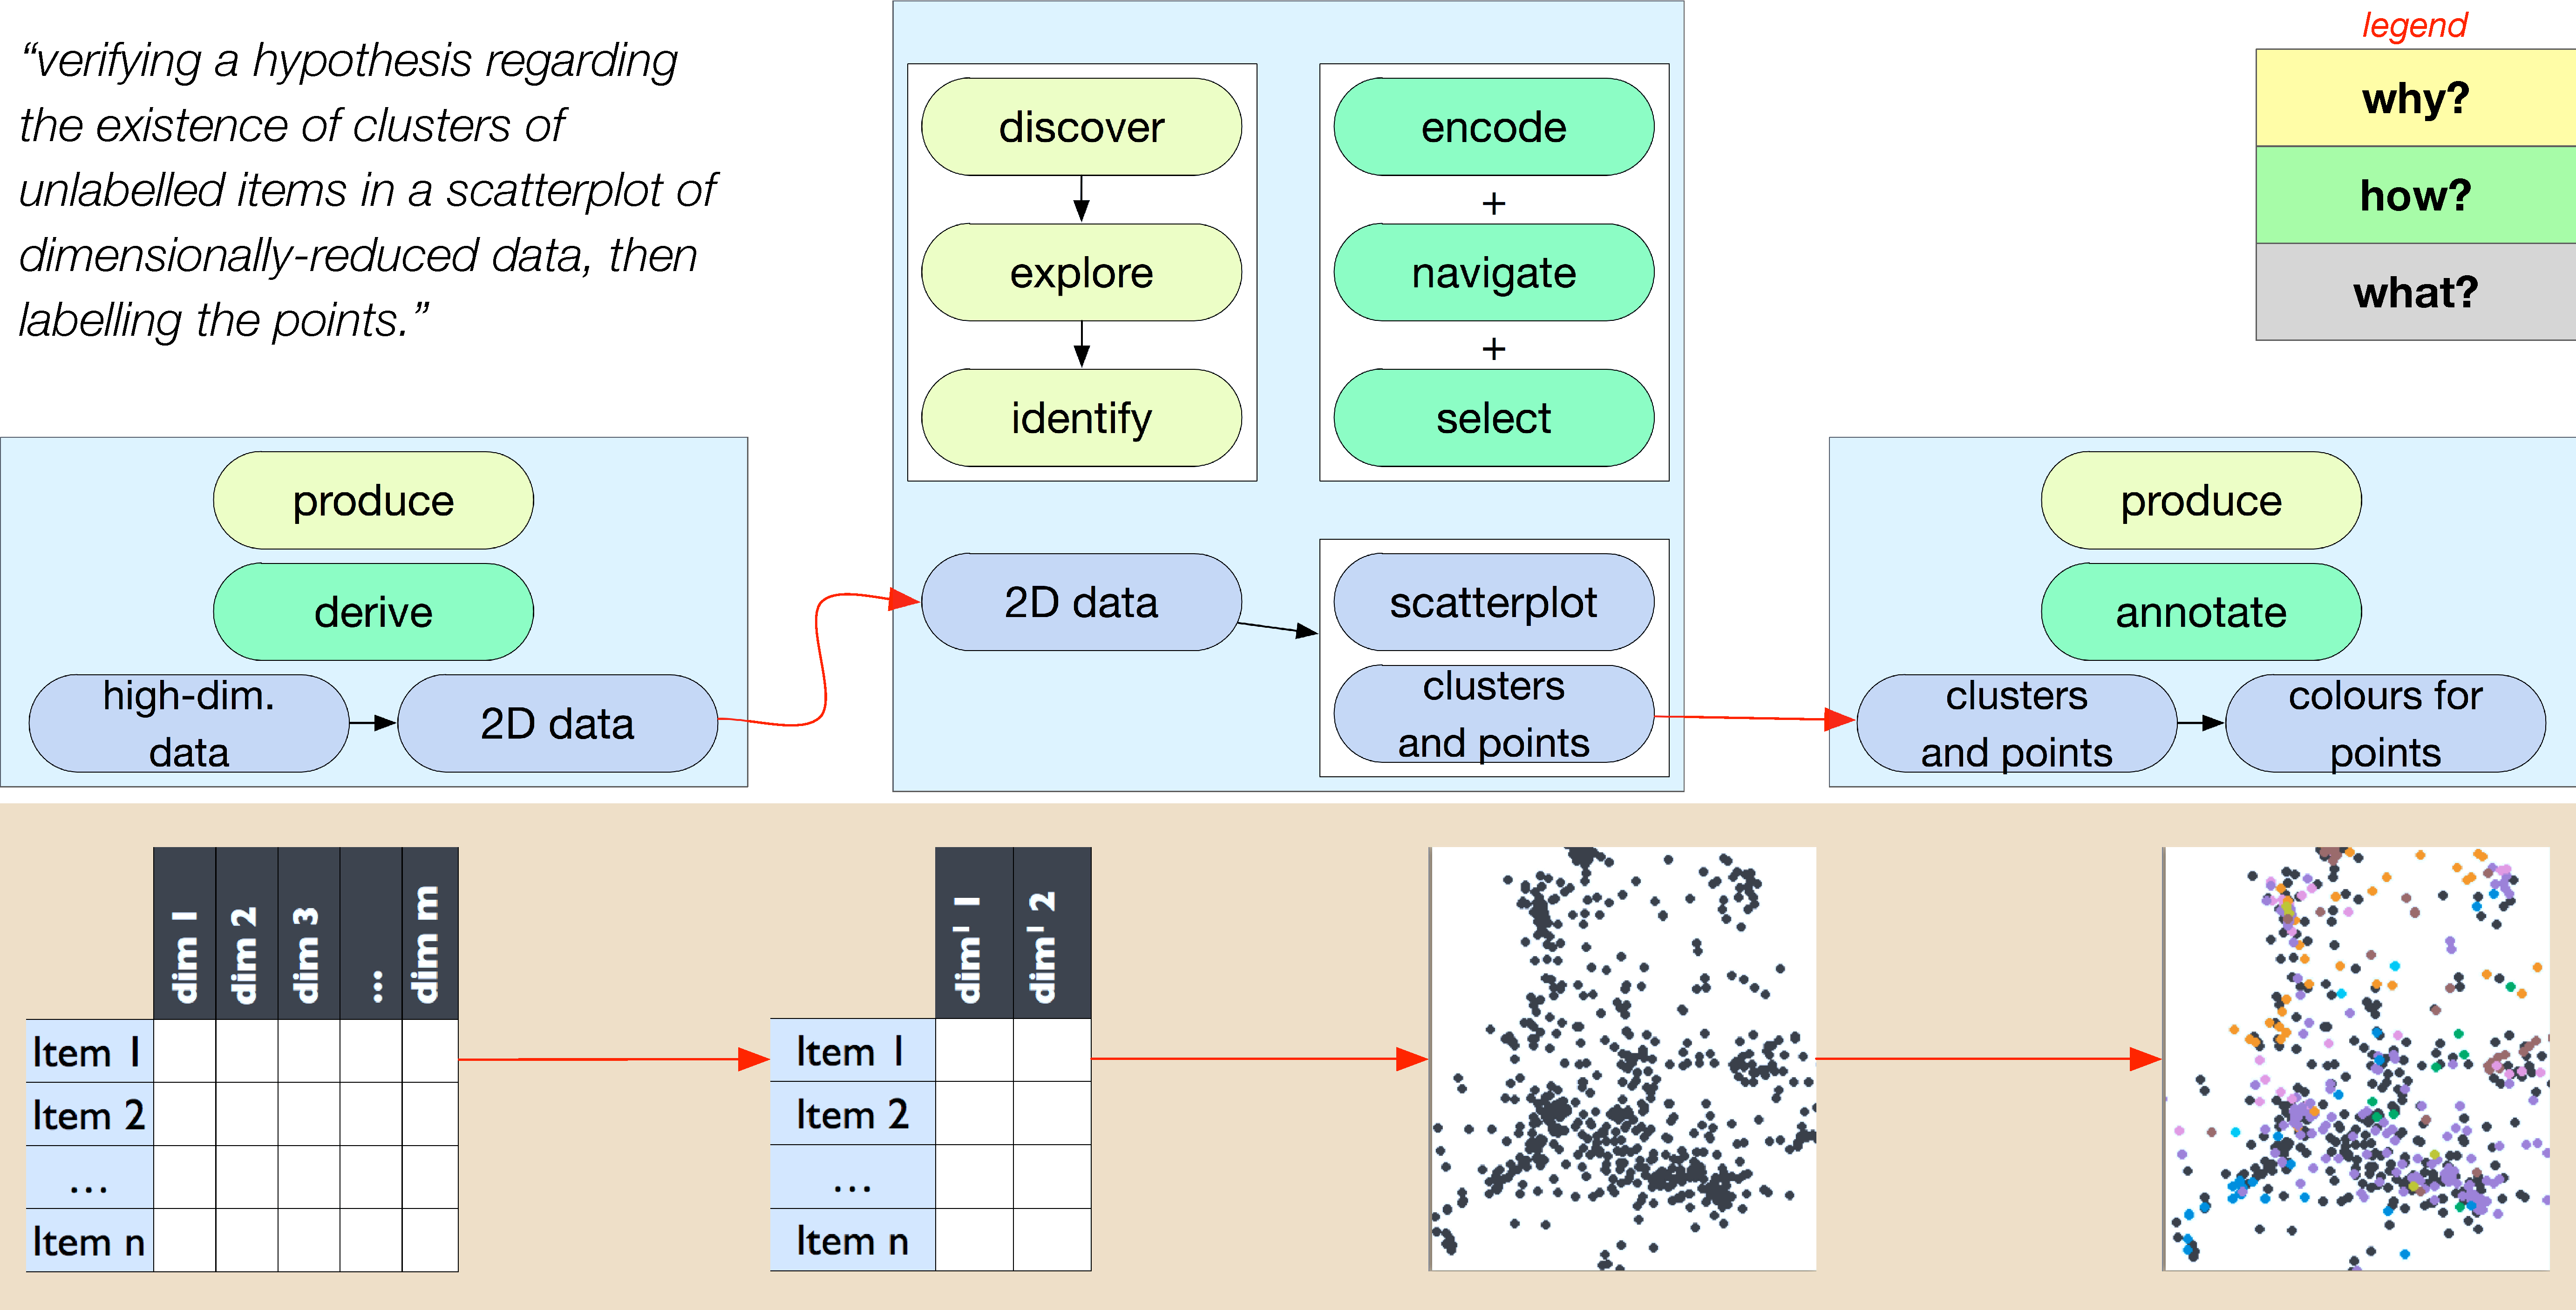
\includegraphics[width=\textwidth]{figures/typology-example.pdf}
    \caption
    [
        An example sequence of tasks as using the structure and vocabulary of our typology.
    ]
    {
        An example sequence of tasks, described as a sentence (top left), as well as using the structure and vocabulary of our typology (top); the bottom depicts a series of transformations corresponding to the {\tt inputs} and {\tt outputs} of each task.
    }
    \label{typology:fig:task_chain}
\end{figure}

%-|-|-|-|-|-|-|-|-|-|-|-|-|-|-|-|-|-|-|-|-|-|-|-|-|-|-|-|-|-|-|-|-|-|-|-|-

Visualization tasks\index{task} are seldom executed in isolation, and the {\tt output}\index{{\tt output}} of one task\index{task} may serve as {\tt input}\index{{\tt input}} to a subsequent task\index{task!task sequence}.
To illustrate this type of dependency, we present an example in which our typology\index{task!task typology} is used to describe a sequence of interdependent tasks\index{task!task sequence}.

Consider the case of labelling clusters of related items in a dataset with many dimensions, where a label is a new categorical attribute value for the item.
Labels are assigned to clusters by means\index{task!means} of {\tt annotation}\index{{\tt annotate}}.
However, one must first {\tt explore}\index{{\tt explore}} the visualized dataset and {\tt identify}\index{{\tt identify}} clusters of interest.
Here a person uses a visualization technique in which items in the dataset are {\tt encoded}\index{{\tt encode}} as points in an interactive scatterplot\index{visual encoding!scatterplot}.
{\tt Identifying}\index{{\tt identify}} clusters is facilitated by {\tt navigating}\index{{\tt navigate}} and {\tt selecting}\index{{\tt select}} items in this scatterplot\index{visual encoding!scatterplot}; upon {\tt selection}\index{{\tt select}}, additional attribute values for the item are shown in details-on-demand\index{view coordination!details-on-demand} secondary displays or in tooltips.
This task\index{task} too has a dependency on the result of an earlier task\index{task}.
Before the the data is {\tt encoded}\index{{\tt encode}} in the scatterplot\index{visual encoding!scatterplot}, a set of two-dimensional distances between data points must be {\tt produced}\index{{\tt produce}}:     they are {\tt derived}\index{{\tt derive}} from the original set of dimensional attributes using \ac{DR}\index{dimensionality reduction (DR)}.

Using our typology\index{task!task typology}, we can express dependencies in which the {\tt output}\index{{\tt output}} of one task\index{task} serves as the {\tt input}\index{{\tt input}} of another, such as the relationship between how data is {\tt derived}\index{{\tt derive}} and the choice of visual encoding\index{visual encoding}.
Such dependencies are represented in \autoref{typology:fig:task_chain}.

As in the examples of \autoref{typology:context}, we can compare our description to those generated by other classifications.
Consider the classification of basic visualization tasks\index{task} by \citet{Chuah1996}, which distinguishes between three categories of {\it operations}.
Using this classification, this sequence of tasks\index{task!task sequence} could be described as having {\it data operations} ({\it derived attributes}\index{{\tt derive}}), {\it graphical operations} ({\it encode data}\index{{\tt encode}}), and {\it set operations} ({\it create set, express membership}).
This description does specify {\it how}\index{{\tt how}} and {\it what}\index{{\tt what}}, but it does not express the interdependencies within a sequence of tasks\index{task!task sequence}, nor does it tell us {\it why}\index{{\tt why}} the data is being visualized.
Neither can we easily distinguish when sets (or clusters) are created, as this might occur before the data is encoded\index{{\tt encode}}, or it might occur via interactive {\tt selection}\index{{\tt select}} of items in the scatterplot\index{visual encoding!scatterplot}.

While the description based on \citet{Chuah1996} classification is atemporal, the {\it operator} {\it interaction} {\it framework} by \citet{Chi1998} defines stage- and transformation- based operators occurring along the visualization pipeline.
Their framework does not contain a comprehensive list of operators, so we draw from the example {\it operators} cited in their paper to describe this sequence of tasks\index{task!task sequence} as follows:

%-|-|-|-|-|-|-|-|-|-|-|-|-|-|-|-|-|-|-|-|-|-|-|-|-|-|-|-|-|-|-|-|-|-|-|-|-

\begin{enumerate}
    \item {\it visualization transformation operators}: \\
    dimension reduction (\ac{DR})\index{dimensionality reduction (DR)}
    
    \item {\it visual mapping transformation operators}: \\
    scatterplot\index{visual encoding!scatterplot}
    
    \item {\it view stage operators}: \\
    zoom, focus, details-on-demand\index{view coordination!details-on-demand}, pick

\end{enumerate}

%-|-|-|-|-|-|-|-|-|-|-|-|-|-|-|-|-|-|-|-|-|-|-|-|-|-|-|-|-|-|-|-|-|-|-|-|-

This description does capture the interdependencies for this sequence of tasks\index{task!task sequence}, though it mischaracterizes the processes of dimension reduction\index{dimensionality reduction (DR)} as transformations to visualized elements, rather than transformations on data, a distinction central to our definition of {\tt derive}\index{{\tt derive}}.
While this description captures up until the second task\index{task} in our description, it does not capture the final task\index{task} of producing cluster labels by means\index{task!means} of annotation\index{{\tt annotate}}.

The description based on our typology retains the separability of these tasks\index{task}, ensuring the distinction between interim {\tt inputs}\index{{\tt input}} and {\tt outputs}\index{{\tt output}}.
Another problem with descriptions generated by existing classifications was that of coverage; the {\it how}\index{{\tt how}} part of our typology includes both {\tt derive}\index{{\tt derive}} and {\tt annotate}\index{{\tt annotate}}, while descriptions generated by other classifications could not account for the latter~\cite{Amar2005,Chi1998}, or both~\cite{Pike2009,Shneiderman1996,Valiati2006,Wehrend1990,Yi2007,Zhou1998}.
Finally, our description also accounts for both {\it why}\index{{\tt why}} data is {\tt derived}\index{{\tt derive}} and {\it why}\index{{\tt why}} clusters are {\tt annotated}\index{{\tt annotate}} with tags, whereas descriptions generated using existing classifications mention {\it how}\index{{\tt how}} a task\index{task} is performed in relation only to {\it when} it is performed~\cite{Chi1998} or to {\it what}\index{{\tt what}} it is performed on~\cite{Chuah1996}.
We maintain that a task\index{task} description requires {\it why}\index{{\tt why}}, {\it how}\index{{\tt how}}, and {\it what}\index{{\tt what}}; the question of {\it when} for a sequence of interdependent tasks\index{task!task sequence} is best served by denoting task\index{task} {\tt input}\index{{\tt input}} and {\tt output}\index{{\tt output}}.

%-------------------------------------------------------------------------
%-------------------------------------------------------------------------

\section{Connections to Previous Work}
\label{typology:rw}

%-------------------------------------------------------------------------
%-------------------------------------------------------------------------

Our typology was informed in part by related work, including existing classifications and established theoretical models, and in part by new thinking with many points of divergence from previous work.
We surveyed work relating to tasks\index{task} spanning the research literature in visualization, visual analytics\index{visual analytics}, \ac{HCI}\index{human-computer interaction (HCI)}, cartography\index{cartography}, and information retrieval\index{information retrieval}.
We focus on two subsets that informed the configuration of our typology: thirty works that explicitly contribute a taxonomy, typology, characterization, framework, or model of tasks\index{task}, goals, objectives, intentions, activities, or interactions~\cite{Amar2005,Amar2004,Andrienko2006,Buja1996,Card1999,Casner1991,Chi1998,Chuah1996,Dix1998,Gotz2008,Heer2012,Keim2002,Klein2006,Lee2006,Liu2010,Mullins1993,Pike2009,Pirolli2005,Raskin2000,Roth2012,Roth2013,Roth1990,Shneiderman1996,Spence2007,Springmeyer1992,Tweedie1997,Valiati2006,Ward2004,Wehrend1990,Yi2007,Zhou1998}\index{interaction}, along with twenty other references that make compelling or noteworthy assertions about the behaviour of people who use visualization tools or techniques~\cite{Aigner2011,Andre2009,Dork2011,Dork2012,Friel2001,Kandel2012,Marchionini2006,Munzner2009a,Plaisant1995,Pousman2007,Roth2012a,Sprague2012,Shrinivasan2008,Stephenson1967,Tory2004,Toms2000,Tukey1977,vanWijk2006,Ware2012,Wilkinson2005}\footnote{\autoref{app:typology} includes additional meta-analysis of this literature and documents the evolution of our typology.}.
The similarities between the individual nodes of our typology and those of existing classifications and other related work are presented in detail in \autoref{typology:tab:rw:why} and \autoref{typology:tab:rw:how}\footnote{\citet{Yalcin2014} has visualized the vocabulary from previous work represented in these tables here: \url{http://keshif.me/demo/vis_tasks.html}.}.

\autoref{typology:tab:rw:why} and \autoref{typology:tab:rw:how} serve three purposes: they document our choices of terms for the purpose of reproducibility, they illustrate the influence of previous work on our thinking, and they indicate overrepresented and underrepresented areas in the literature, such as {\tt consume}\index{{\tt consume}} and {\tt enjoy}\index{{\tt enjoy}} in the {\it why}\index{{\tt why}} part of our typology.
Note that non-leaf nodes in the {\it how}\index{{\tt how}} part of our typology are poorly represented, serving to indicate the gap between low and high levels of abstraction\index{task!task abstraction}.

%-|-|-|-|-|-|-|-|-|-|-|-|-|-|-|-|-|-|-|-|-|-|-|-|-|-|-|-|-|-|-|-|-|-|-|-|-

\begin{table}\renewcommand{\arraystretch}{1.2}\addtolength{\tabcolsep}{-1pt}
    \begin{center}
    \tiny
    \begin{tabular}{p{0.125\textwidth}>{\RaggedRight}p{0.8\textwidth}}
    
    \rowcolor{yellow!20} 
    
        \multicolumn{2}{c}{\it why?} 
        
    \\
    
    \hline
    
    \rowcolor{blue!10}
    
        {\tt consume}\index{{\tt consume}} & --
    
    \\
    
        {\tt $\rightarrow$ present}\index{{\tt present}} &
    
        	{\it \underline{present}},~\cite{Shrinivasan2008,vanWijk2006}, %Dibiase1990,
        	{\it author, compose}~\cite{Card1999}*,
        	{\it build (case), tell (story)}~\cite{Pirolli2005}*,
        	{\it depict}~\cite{Pike2009}*,
        	{\it express (ideas), describe}~\cite{Springmeyer1992}*,
        	{\it guide, share}~\cite{Heer2012}*
        	{\it inform, elaborate}~\cite{Zhou1998}*,
        	{\it report}~\cite{Kandel2012},
    
    \\ \rowcolor{gray!10}
    
        {\tt $\rightarrow$ discover (generate\index{{\tt discover}}, verify\index{{\tt discover}} hypotheses)}\index{{\tt discover}} &
    
        	{\it \underline{discover}}~\cite{Marchionini2006}, %Dibiase1990,
        	{\it explore}~\cite{Zhou1998}*, \cite{vanWijk2006},
        	{\it verify}~\cite{Casner1991}*, \cite{Marchionini2006},
        	{\it synthesize}~\cite{Mullins1993}*, \cite{Marchionini2006}, %Dibiase1990,
        	{\it investigate, integration (of insight)}~\cite{Springmeyer1992}*, \cite{Marchionini2006},
        	{\it frame operations: construct, elaborate, question, reframe}~\cite{Klein2006}*,
        	{\it assimilate, assess, understand}~\cite{Pike2009}*,
        	{\it infer}~\cite{Valiati2006}*,
        	{\it analyze}~\cite{Mullins1993,Pike2009}*, \cite{Marchionini2006},
        	{\it support, reevaluate (hypotheses)}~\cite{Pirolli2005}*, %Dibiase1990,
        	{\it monitoring}~\cite{Ware2012},
        	{\it confirm (hypotheses)},
        	{\it expose (uncertainty)},
        	{\it formulate (cause and effect)},
        	{\it concretize (relationships)},
        	{\it learn (domain parameters)},
        	{\it multivariate explanation}~\cite{Amar2004}*,
        	{\it evaluate, learn, investigate}~\cite{Marchionini2006},
        	{\it open-ended exploration, diagnosis}~\cite{Plaisant1995},
        	{\it abduction, deduction, induction}~\cite{Pike2009},
        	{\it generate, confirm (hypotheses)}~\cite{Andre2009,Friel2001}, %Dibiase1990,
        	{\it integrate, interpret}~\cite{Friel2001},
        	{\it exploratory and confirmatory data analysis}~\cite{Tukey1977} %Dibiase1990,
    
    \\
    
        {\tt $\rightarrow$ enjoy}\index{{\tt enjoy}} &
    
    	    (using visualized data in casual contexts)~\cite{Pousman2007,Sprague2012},
    	    {\it strolling}~\cite{Dork2012}
    
    \\ \rowcolor{blue!10}
    
        {\tt produce}\index{{\tt produce}} &
    
        	{\it export}~\cite{Roth2012,Roth2013}*,
        	{\it store}~\cite{Mullins1993}*,
        	{\it save}~\cite{Liu2010,Roth2012,Roth2013}*,
        	{\it extract}~\cite{Card1999,Shneiderman1996}*,
        	{\it generating (images)}~\cite{Plaisant1995},
        	(a {\it classification})~\cite{Card1999,Springmeyer1992}*,
        	(a {\it categorization})~\cite{Mullins1993,Wehrend1990,Zhou1998}*,
        	%{\it names (for clusters)}~\cite{Sedlmair2012}*,
        	(a {\it record} of one's history / process)~\cite{Heer2012,Shneiderman1996,Springmeyer1992}*
        	
        
    
    \\  \hline \rowcolor{blue!10} 
    
        {\tt search}\index{{\tt search}} &
    
            {\it \underline{search}}~\cite{Card1999,Pirolli2005,Zhou1998}*,
            {\it acquire}~\cite{Mullins1993}*,
            {\it visual queries}~\cite{Ware2012}
    
    \\
    
        {\tt $\rightarrow$ lookup}\index{{\tt lookup}} &
    
        	{\it \underline{lookup}}~\cite{Casner1991}*~\cite{Marchionini2006},
        	{\it identify: lookup (value)}~\cite{Wehrend1990}*,
        	{\it (value) lookup}~\cite{Roth1990}*,
        	{\it retrieve (value)}~\cite{Amar2005,Lee2006,Pike2009,Roth2012,Roth2013}*\cite{Tory2004},
        	{\it procure}~\cite{Roth2012,Roth2013}*
    
    \\ \rowcolor{gray!10}
    
        {\tt $\rightarrow$ browse}\index{{\tt browse}} &
    
            {\it \underline{browse}}~\cite{Card1999,Mullins1993,Pike2009,Spence2007}*, \cite{Dork2012,Toms2000}, %Tufte1997},
        	{\it search}~\cite{Roth2012,Roth2013}*, %Roth's definition of search = browse
        	{\it finding (gestalt)}~\cite{Buja1996}*,
        	{\it browsing tasks: follow (path)}~\cite{Lee2006}*
    
    \\
    
        {\tt $\rightarrow$ locate}\index{{\tt locate}} &
    
            {\it \underline{locate}}~\cite{Liu2010,Mullins1993,Valiati2006,Wehrend1990,Zhou1998}*, \cite{Friel2001},
        	{\it search}~\cite{Casner1991}*\cite{Dork2012},
        	{\it search (for known item)}~\cite{Marchionini2006},
        	{\it seek}~\cite{Spence2007}*,
        	{\it pathfinding}~\cite{Ware2012}
    
    \\ \rowcolor{gray!10}
    
        {\tt $\rightarrow$ explore}\index{{\tt explore}} &
    
        	{\it \underline{explore}}~\cite{Liu2010,Pike2009,Yi2007}*, \cite{Ware2012,Wilkinson2005}, %explore as search
        	{\it forage}~\cite{Card1999,Liu2010,Pirolli2005}*,
        	{\it finding (gestalt)}~\cite{Buja1996}*,
        	{\it (overview) tasks}~\cite{Lee2006}*,
        	{\it find (clusters, correlations, extremum, anomalies)}~\cite{Amar2005,Lee2006,Pike2009}*,
        	{\it determine (correlations)}~\cite{Roth1990}*,
        	{\it determine (clusters)}~\cite{Wehrend1990}*
        	
        
        
    \\ \hline \rowcolor{blue!10} 
    
        {\tt query}\index{{\tt query}} &
    
        	{\it \underline{query}}~\cite{Raskin2000}*,
        	{\it posing queries}~\cite{Buja1996}*,
        	{\it elementary and synoptic tasks}~\cite{Andrienko2006}*,
        	{\it levels of questions}~\cite{Tweedie1997}*,
        	{\it question answering}~\cite{Marchionini2006}
    
    \\
    
        {\tt $\rightarrow$ identify}\index{{\tt identify}}  &
    
        	{\it \underline{identify}}~\cite{Lee2006,Mullins1993,Pike2009,Roth2012,Roth2013,Valiati2006,Wehrend1990,Zhou1998}*, \cite{Roth2012,Roth2013},
        	{\it reading (the data)}~\cite{Friel2001},
        	{\it read (fact, pattern)}~\cite{Card1999}*,
        	{\it lookup}~\cite{Andrienko2006}*,
        	{\it examine}~\cite{Springmeyer1992}*,
        	{\it determine (range)}~\cite{Amar2005,Lee2006,Pike2009}*,
        	{\it determine / characterize (distribution)}~\cite{Amar2005,Lee2006,Pike2009,Wehrend1990}*,
        	{\it recognize}~\cite{Klein2006}*
    
    \\ \rowcolor{gray!10}
    
        {\tt $\rightarrow$ compare}\index{{\tt compare}} &
    
        	{\it \underline{compare}}~\cite{Andrienko2006,Klein2006,Mullins1993,Pike2009,Roth2012,Roth2013,Springmeyer1992,Valiati2006,Zhou1998}*, \cite{Marchionini2006},
        	{\it compare (within a relation vs. across / between relations)}~\cite{Roth1990,Wehrend1990}*,
        	{\it relation seeking}~\cite{Andrienko2006}*,
        	{\it read comparison}~\cite{Card1999}*,
        	{\it making comparisons}~\cite{Buja1996}*,~\cite{Ware2012},
        	{\it discriminate}~\cite{Mullins1993}*, %\cite{Tufte1997}
        	{\it associate}~\cite{Roth2012,Roth2013}* %\cite{Tufte1997}
        %		{\it match}~\cite{Sedlmair2012}*%\cite{Tufte1997}
    
    \\
    
        {\tt $\rightarrow$ summarize}\index{{\tt summarize}} &
    
        	{\it \underline{summarize}}~\cite{Zhou1998}*, %Tufte1997},
        	{\it summarize (set), enumerate (set objects)}~\cite{Chuah1996}*,
        	{\it overview}~\cite{Card1999,Dix1998,Shneiderman1996}*,
        	{\it (overview) tasks}~\cite{Lee2006}*,
        	{\it scan}~\cite{Lee2006,Mullins1993}*,
        	{\it connectional tasks}~\cite{Andrienko2006}*,
        	{\it count}~\cite{Lee2006,Shneiderman1996}*,
        	{\it visualization}~\cite{Dork2012},
        	{\it review}~\cite{Shrinivasan2008}
    \\
    
    \end{tabular}
    
    \caption
    [
        Nodes in the \textsl{why} part of our typology and their relation to the vocabulary used in previous work.
    ]
    {
        Nodes in the \textsl{why} part of our typology of abstract visualization tasks and their relation to the vocabulary used in previous work.
        Underlining is used where a term used in our typology appears in related work.
        Terms in parentheses are encompassed by the \textsl{what} part of our typology.
        Previous work that explicitly contributes a classification system is denoted by *; other sources incidentally make compelling or noteworthy assertions about the use of visualization tools or techniques.
    }
    
    \label{typology:tab:rw:why}
    \end{center}
\end{table}

%-|-|-|-|-|-|-|-|-|-|-|-|-|-|-|-|-|-|-|-|-|-|-|-|-|-|-|-|-|-|-|-|-|-|-|-|-

%-|-|-|-|-|-|-|-|-|-|-|-|-|-|-|-|-|-|-|-|-|-|-|-|-|-|-|-|-|-|-|-|-|-|-|-|-
    	
\begin{table}\renewcommand{\arraystretch}{1.2}\addtolength{\tabcolsep}{-1pt}
    \begin{center}
    \tiny
    \begin{tabular}{p{0.125\textwidth}>{\RaggedRight}p{0.8\textwidth}}
    
    \rowcolor{green!20} 
    
        \multicolumn{2}{c}{\it how?} 
        
    \\
    
    \hline \rowcolor{blue!10}
    
        {\tt encode}\index{{\tt encode}} &
    
        	{\it \underline{encode}}~\cite{Chuah1996,Pike2009,Yi2007,Zhou1998}*,
        	{\it create mapping}~\cite{Chuah1996}*,
        	{\it visualize}~\cite{Heer2012,Valiati2006}*,
        	{\it generate}~\cite{Springmeyer1992}*,
        	{\it transform (visual mapping)}~\cite{Chi1998}*
    
    \\ \hline \rowcolor{blue!10} 
        
        {\tt manipulate}\index{{\tt manipulate}} &
    
        	{\it \underline{manipulate}}~\cite{Wilkinson2005},
        	{\it (object) manipulation}~\cite{Mullins1993}*,
        	{\it modify}~\cite{Raskin2000}*,
        	{\it (data) manipulation loop}~\cite{Ware2012}
    
    \\
    
        {\tt $\rightarrow$ select}\index{{\tt select}} &
    
        	{\it \underline{select}}~\cite{Heer2012,Mullins1993,Pike2009,Raskin2000,Ward2004,Yi2007}*, %\cite{Tufte1997},
        	{\it brush}~\cite{Gotz2008,Keim2002,Pike2009}*, \cite{Chi1998,Ware2012,Wilkinson2005},
        	{\it distinguish}~\cite{Wehrend1990,Zhou1998}*, %\cite{Tufte1997},
        	{\it emphasize}~\cite{Zhou1998}*,
        	{\it differentiate}~\cite{Pike2009}*,
        	{\it highlight}~\cite{Dix1998,Heer2012,Raskin2000}*, \cite{Ware2012}, %\cite{Tufte1997},
        	{\it identify: portray, individualize, profile}~\cite{Zhou1998}*, %in our why taxonomy
        	{\it indicate}~\cite{Mullins1993,Raskin2000}*,
        	{\it mark}~\cite{Mullins1993,Yi2007}*,
        	{\it reference}~\cite{Mullins1993}*,
        	{\it outline (clusters)}~\cite{Zhou1998}*,
        	{\it promote}~\cite{Card1999}*,
        	{\it track}~\cite{Yi2007}*,
        	%{\it choose, isolate, single out}~\cite{Tufte1997},
        	{\it pick}~\cite{Mullins1993}*\cite{Chi1998},
        	{\it express (set membership)}~\cite{Chuah1996}*
        	{\it connect}~\cite{Pike2009,Yi2007}*
    
    \\ \rowcolor{gray!10}
    
        {\tt $\rightarrow$ navigate}\index{{\tt navigate}} &
    
        	{\it \underline{navigate}}~\cite{Heer2012,Spence2007,Ward2004}*, \cite{Marchionini2006,Munzner2009a,Plaisant1995,Ware2012,Wilkinson2005},
        	{\it focus}~\cite{Buja1996,Dix1998}*, \cite{Chi1998}, %\cite{Tufte1997},
        	{\it details-on-demand}~\cite{Card1999,Shneiderman1996}*, \cite{Chi1998},
        	{\it flip through}~\cite{Chi1998},
        	{\it zoom}~\cite{Buja1996,Card1999,Dix1998,Gotz2008,Keim2002,Mullins1993,Pike2009,Roth2012,Roth2013,Shneiderman1996,Yi2007}*, \cite{Chi1998,Munzner2009a,Wilkinson2005},
        	{\it pan}~\cite{Buja1996,Gotz2008,Mullins1993,Pike2009,Roth2012,Roth2013,Yi2007}*, \cite{Wilkinson2005},
        	{\it elaborate}~\cite{Pike2009,Yi2007}*,
        	{\it abstract}~\cite{Pike2009,Yi2007}*, %\cite{Tufte1997},
        	{\it change (range)}~\cite{Gotz2008}*,
        	{\it drill down}~\cite{Dix1998}*,
        	{\it maneuver / navigate}~\cite{Springmeyer1992}*,
        	{\it rotate}~\cite{Chi1998,Wilkinson2005}
        	{\it revisit}~\cite{Gotz2008,Lee2006}*
    
	\\
    
        {\tt $\rightarrow$ arrange}\index{{\tt arrange}} &
    
        	{\it \underline{arrange}}~\cite{Buja1996,Roth2012,Roth2013}*,
        	{\it sort}~\cite{Amar2005,Gotz2008,Heer2012,Lee2006,Pike2009}*, \cite{Munzner2009a},
        	{\it rank}~\cite{Roth2012,Roth2013,Wehrend1990,Zhou1998}*,
        	{\it coordinate}~\cite{Heer2012}*,
        	{\it delineate, sequence}~\cite{Roth2012,Roth2013}*,
        	{\it index}~\cite{Roth1990}*,
        	{\it move}~\cite{Mullins1993,Raskin2000}*,
        	{\it edit}~\cite{Mullins1993}*, %\cite{Tufte1997},
        	{\it organize}~\cite{Heer2012}*, ~\cite{Shrinivasan2008}, %\cite{Tufte1997},
        	{\it orient, permute, position, translate}~\cite{Chi1998},
        	%{\it structure}~\cite{Tufte1997},
        	{\it reorder}~\cite{Card1999,Wilkinson2005},
        	{\it configure}~\cite{Valiati2006}*,
        	{\it reconfigure}~\cite{Pike2009,Yi2007}*,
        	{\it restructure}~\cite{Liu2010}*
    
    \\ \rowcolor{gray!10}
    
        {\tt $\rightarrow$ change}\index{{\tt change}} &
    
        	{\it change (parameters)}~\cite{Dix1998}*, ~\cite{Chi1998},
        	{\it change (metaphor)}~\cite{Gotz2008}*,
        	{\it change (representation)}~\cite{Dix1998}*,
        	{\it change (vis. encoding)}~\cite{Munzner2009a},
        	{\it transform}~\cite{Raskin2000}*, \cite{Marchionini2006,Wilkinson2005},
        	{\it transform (mapping), shift, scale, set (graphical value)}~\cite{Chuah1996}*,
        	{\it rotate, scale}~\cite{Chi1998},
        	{\it configure}~\cite{Valiati2006}*,
        	{\it animate}~\cite{Chi1998,Wilkinson2005},
        	{\it distort}~\cite{Keim2002,Ward2004}*~\cite{Chi1998},
        	{\it orient / transform}~\cite{Springmeyer1992}*,
        	{\it (object) manipulation: transform, stretch, shape}~\cite{Mullins1993}*,
        	{\it re-express},
        	{\it re-symbolize},
        	{\it re-project}~\cite{Roth2012,Roth2013}*,
        	{\it edit}~\cite{Mullins1993,Roth2012,Roth2013}*,
        	%{\it refine}~\cite{Sedlmair2012}*,
        	{\it activate}~\cite{Raskin2000}*
    
    \\
    
        {\tt $\rightarrow$ filter}\index{{\tt filter}} &
    
        	{\it \underline{filter}}~\cite{Amar2005,Card1999,Gotz2008,Heer2012,Keim2002,Klein2006,Lee2006,Mullins1993,Pike2009,Pirolli2005,Roth2012,Roth2013,Shneiderman1996,Yi2007}*, \cite{Munzner2009a,Tory2004,Wilkinson2005}, %\cite{Tufte1997}
        	{\it subsetting, (value) filtering, (view) filtering}~\cite{Chi1998},
        	{\it exclude}~\cite{Marchionini2006,Tory2004},
        	{\it screen: filter, suppress, conceal}~\cite{Mullins1993}*, %\cite{Tufte1997},
        	{\it maneuver: (data) management / culling}~\cite{Springmeyer1992}*,
        	{\it configure}~\cite{Valiati2006}*,
        	{\it delete (objects, sets, graphical objects)}~\cite{Chuah1996}*,
        	{\it delete}~\cite{Card1999,Gotz2008,Raskin2000}*,
        	{\it overlay}~\cite{Roth2012,Roth2013}*,
        	{\it restore}~\cite{Gotz2008,Mullins1993}*
        	%{\it reduce, winnow}~\cite{Tufte1997}
    
    \\ \rowcolor{gray!10}
    
        {\tt $\rightarrow$ aggregate}\index{{\tt aggregate}} &
    
        	{\it \underline{aggregate}}~\cite{Mullins1993}*, \cite{Chi1998,Munzner2009a}, %Tufte1997},
        	{\it cluster}~\cite{Card1999}*, \cite{Chi1998}, %Tufte1997},
        	{\it associate}~\cite{Mullins1993,Wehrend1990,Zhou1998}*,
        	{\it simplify}~\cite{Chi1998},
        	{\it link}~\cite{Buja1996,Dix1998,Keim2002,Mullins1993}*, \cite{Shrinivasan2008,Wilkinson2005},
        	{\it merge}~\cite{Gotz2008}*, %\cite{Tufte1997},
        	{\it generalize / merge}~\cite{Zhou1998}*,
        	{\it assemble}~\cite{Mullins1993}*,
        	{\it create (set)}~\cite{Chuah1996}*, %\cite{Tufte1997},
        	%{\it group}~\cite{Sedlmair2012}*,
        	{\it split}~\cite{Gotz2008}*,
        	{\it disassemble}~\cite{Mullins1993}*,
        	{\it disassociate}~\cite{Mullins1993}*,
        	{\it reveal: itemize, separate}~\cite{Zhou1998}*,
        	{\it segregate: ungroup, unlink}~\cite{Mullins1993}*,
        	{\it withdraw, overlay}~\cite{Mullins1993}*
    
    \\ \hline \rowcolor{blue!10} 
    
        {\tt introduce} &
    
    	    {\it \underline{introduce}}~\cite{Mullins1993}*
    
    \\
    
        {\tt $\rightarrow$ annotate}\index{{\tt annotate}} &
    
        	{\it \underline{annotate}}~\cite{Gotz2008,Heer2012,Roth2012,Roth2013}*,
        	{\it add placemark}~\cite{Yi2007},
        	{\it create (anchors)}~\cite{Liu2010}*,
        	{\it create / copy (graphical objects)}~\cite{Chuah1996}*,
        	{\it create / modify (note)}~\cite{Gotz2008}*,
        	{\it externalize (analysis artefacts)}~\cite{Shrinivasan2008},
        	{\it give a meaningful name to (groups / clusters)}~\cite{Lee2006}*
    
    \\ \rowcolor{gray!10}
    
        {\tt $\rightarrow$ import}\index{{\tt import}} &
    
        	{\it \underline{import}}~\cite{Roth2012,Roth2013}*,
        	{\it add (objects)}~\cite{Chuah1996}*,
        	{\it create}~\cite{Card1999,Mullins1993}*,
        	{\it generate}~\cite{Raskin2000}*,
        	{\it (data) entry}~\cite{Mullins1993}*,
        	{\it load}~\cite{Liu2010}
    
    \\
    
        {\tt $\rightarrow$ derive}\index{{\tt derive}} &
    
        	{\it \underline{derive}}~\cite{Heer2012}*,
        	{\it derived (attributes)}~\cite{Chuah1996}*,
        	{\it derive (new conditions)}~\cite{Springmeyer1992}*,
        	{\it compute (derived value)}~\cite{Amar2005,Lee2006,Pike2009}*,
        	{\it copy}~\cite{Raskin2000}*,
        	{\it compute}~\cite{Zhou1998}*,
        	{\it calculate}~\cite{Mullins1993,Roth2012,Roth2013,Springmeyer1992}*,
        	{\it configure, determine}~\cite{Valiati2006}*, %also appears in select
        	{\it average}~\cite{Card1999}*,
        	{\it computation operators}~\cite{Casner1991}*,
        	{\it transform (data)}~\cite{Chi1998}*,
        	{\it estimate, generate (statistics)}~\cite{Springmeyer1992}*,
        	{\it extrapolate}~\cite{Mullins1993}, *\cite{Friel2001},
        	{\it interpolate}~\cite{Mullins1993}, *\cite{Friel2001}
    
    \\ \rowcolor{gray!10}
    
        {\tt $\rightarrow$ record}\index{{\tt record}} &
    
        	{\it \underline{record}}~\cite{Heer2012,Mullins1993,Springmeyer1992}*,
        	{\it bookmark}~\cite{Gotz2008}*,
        	{\it history}~\cite{Shneiderman1996}*,
        	{\it redo, undo}~\cite{Gotz2008,Yi2007}*
    
    \\
    
    \end{tabular}
    
    \caption
    [
        Nodes in the \textsl{how} part of our typology and their relation to the vocabulary used in previous work.
    ]
    {
        Nodes in the \textsl{how} part of our typology and their relation to the vocabulary used in previous work.
        Typographic conventions follow those used in \autoref{typology:tab:rw:why}.
    }
    \label{typology:tab:rw:how}
    \end{center}
\end{table}

%-|-|-|-|-|-|-|-|-|-|-|-|-|-|-|-|-|-|-|-|-|-|-|-|-|-|-|-|-|-|-|-|-|-|-|-|-


%-------------------------------------------------------------------------

\subsection{Existing Classifications}
\label{typology:rw:taxonomies}

%-------------------------------------------------------------------------


The scope of existing classifications can be categorized in three different ways: level of abstraction\index{task!task abstraction}, temporality, and applicability\index{task!task applicability}.

\bstart{Level of abstraction}
Much of previous work can be divided into those having a low\index{task!low-level tasks} or high level\index{task!high-level tasks} of abstraction\index{task!task abstraction}, with very little falling in between.
Relying solely on either type of classification leads to the aforementioned ends-means\index{task!ends}\index{task!means} confusion, thereby limiting the potential for rigorous analysis.
Low-level\index{task!low-level tasks} use of a visualization technique or tool is well represented in related work~\cite{Amar2005,Andrienko2006,Buja1996,Casner1991,Chi1998,Chuah1996,Dix1998,Gotz2008,Keim2002,Lee2006,Roth1990,Shneiderman1996,Tweedie1997,Valiati2006,Ward2004,Wehrend1990,Yi2007,Zhou1998}.
Elements common to many of these classifications include {\it select}\index{{\tt select}}, {\it filter}\index{{\tt filter}}, and {\it navigate}\index{{\tt navigate}}.
Following \citet{Lee2012} and \citet{Roth2013}, we note that low-level\index{task!low-level tasks} classifications of tasks\index{task} are often conflated with those of interaction\index{interaction} design choices.
At the high level\index{task!high-level tasks}, abstract tasks\index{task!task abstraction} can be found in the context of theoretical models, but without explicit connections to low-level visualization tasks~\cite{Amar2004,Card1999,Klein2006,Liu2010,Pirolli2005}\index{task!low-level tasks}.
Examples of these include {\it confirm hypotheses}, {\it present}\index{{\tt present}}, and {\it explore}\index{{\tt explore}}.
Low-level\index{task!low-level tasks} classifications often provide a sense of {\it how}\index{{\tt how}} a task\index{task} is performed, but not {\it why}\index{{\tt why}}; high-level\index{task!high-level tasks} models are the converse.
Our focus on multi-level descriptions of visualization tasks\index{task} is intended to close this gap and resolve the ends-means\index{task!ends} confusion.

\bstart{Temporality}
Most classifications are atemporal in that they do not have any way to express sequences or dependencies between different stages\index{task!task sequence}.
A few classifications are explicitly temporal in that they divide the behavior of people who use visualization tools or techniques into larger stages that occur in specific sequences or cycles\index{task!task sequence}.
Examples include pipeline models for visualization construction~\cite{Chi1998} or data analysis~\cite{Kandel2012}, or cyclic models such as knowledge crystallization~\cite{Card1999} or information foraging\index{information foraging} and sensemaking~\cite{Pirolli2005}\index{sensemaking}.
However, empirical observations of the use of visualization tools and techniques have indicated a mismatch between the specific cyclical or sequential patterns proposed by these models and the actual behaviour of people~\cite{Isenberg2008a}.
Vicente argues that sequence-based approaches to task analysis\index{task!task analysis} are overly rigid and thus inappropriate for describing such open-ended tasks~\cite{Vicente1999}, and that {\it constraint}-based approaches to task analysis\index{task!task analysis} allow for more flexibility in terms of {\it how}\index{{\tt how}} a task\index{task} is performed.
Descriptions based on our typology do not force any strict {\it global} temporal orderings, as imposed by sequence- or cycle-based models; instead, they accommodate {\it local} interdependencies within sequences of tasks\index{task!task sequence} by way of {\it constraints} on task\index{task} {\tt input}\index{{\tt input}} and {\tt output}\index{{\tt output}}.

\bstart{Applicability}
Many classifications represented in our survey are applicable across domains and datatypes, though specifically-targeted classifications and models do exist.
Examples include Lee~\etal's task\index{task} taxonomy for graph visualization~\cite{Lee2006} and Lammarsch~\etal's task\index{task} framework for time-oriented data~\cite{Lammarsch2012}. 
Our typology encompasses and complements these specific classifications, and we encourage further development of more like these.
%RR: p.39, bottom: - "General vs. specific" - might be more accurate to have this label be "General vs. specific applicability" (or even just "Applicability").

We are also aware of five domain- and datatype-agnostic classifications that span low-level\index{task!low-level tasks} and high-level tasks\index{task!high-level tasks}.
These classifications had the highest contributions to the organization of our own typology:

\bstart{\citet{Springmeyer1992} (1992)}
This classification of scientific data analysis covers both {\it how}\index{{\tt how}} and {\it why}\index{{\tt why}}, but these aspects are not clearly distinguished within its hierarchical structure, that which begins with a high-level\index{task!high-level tasks} distinction between {\it investigation} and {\it integration of insight}\index{insight}.

\bstart{\citet{Mullins1993} (1993)}
This extensive taxonomy contains over 150 items: an exhaustive list of high-level\index{task!high-level tasks} {\it mediation} and {\it coordination} tasks\index{task}, which overlaps with our classification of {\it why}\index{{\tt why}} and {\it how}\index{{\tt how}}, as well as many low-level\index{task!low-level tasks} object-oriented interactions\index{interaction} relating to physical interface {\tt input}\index{{\tt input}} and {\tt output}\index{{\tt output}}.
We do not attempt to specify tasks\index{task} at this lowest level, though we have adopted a consideration of {\tt input}\index{{\tt input}} and {\tt output}\index{{\tt output}} in the {\it what}\index{{\tt what}} part of our typology.

\bstart{\citet{Pike2009} (2009)}
Their characterization of {\it analytic discourse} draws from earlier work, distinguishing high-level\index{task!high-level tasks} modes of inquiry~\cite{Amar2004} as {\it goals}, from low-level tasks~\cite{Amar2005}\index{task!low-level tasks} and interactions~\cite{Yi2007}\index{interaction}.
These are in turn distinguished from the separable {\it intents} of representation and interaction\index{interaction} design choices.
Bringing these formerly disjoint classifications together is laudable, though the integration of this information for the purpose of analyzing tasks\index{task} was not the focus of Pike \etal's article.
The aim of our typology of abstract tasks\index{task} is to make this integration explicit, relating these intents and design choices ({\it how}\index{{\tt how}}) to modes of inquiry, goals, and tasks\index{task} ({\it why}\index{{\tt why}}).

\bstart{\citet{Heer2012} (2012)}
Their {\it taxonomy of interaction dynamics} provides a top-level distinction between {\it data}-, {\it view}-, and {\it process}-centric tasks\index{task}.
The focus of their taxonomy is on interactive elements and operations; ten of the twelve task\index{task} types they characterize are encompassed by the {\it how}\index{{\tt how}} part of our typology.
The two remaining {\it process and provenance\index{analytical provenance}} tasks\index{task}, {\it share} and {\it guide}, are captured by the definition of {\tt present}\index{{\tt present}} in the {\it why}\index{{\tt why}} part of our typology.

\bstart{\citet{Roth2013} (2012)}
Roth's taxonomy, based on Norman's {\it Stages of Action} model \cite{Norman1988}\index{stages of action (Norman)}, classifies {\it cartographic interaction primitives}\index{cartography} as {\it objectives}, {\it operators}, and {\it operands}.
Norman's model describes a series of translations between a person's goal, an immediate intention (or {\it objective}), and a series of actions ({\it operators}) performed on an environment (of {\it operands}).
Roth's classification is closely aligned with our notions of {\it why}\index{{\tt why}}, {\it how}\index{{\tt how}}, and {\it what}\index{{\tt what}}, and thus has a high-level structure similar to that of our own typology.
However, Roth's taxonomy imposes a spatial constraint on where {\it operands} are located in space, as discussed in \autoref{typology:context}.
In contrast, we restrict our classification of {\it what}\index{{\tt what}} to that of {\tt input}\index{{\tt input}} and {\tt output}\index{{\tt output}}; the location of {\it operands} is represented by the {\tt search}\index{{\tt search}} node in the {\it why}\index{{\tt why}} part of our typology.

What these five classifications have in common is that they are atemporal, and most span our characterization of {\it why}\index{{\tt why}} and {\it how}\index{{\tt how}}.
Our typology integrates and extends this work, adding a specification of {\it what}\index{{\tt what}}, the {\tt input}\index{{\tt input}} and {\tt output}\index{{\tt output}} of tasks\footnote{As indicated in \autoref{typology:what}, we chose a flexible and agnostic representation of {\it what} the {\tt inputs} and {\tt outputs} can be. \citet{Munzner2014} has since provided a more structured classification of {\it targets} that can be used in the analysis of the {\tt outputs} of tasks; for more detail about this extension to the typology, see \autoref{conclusions:typology}.}\index{task}.
As a result, our typology can be used to describe sequences of tasks\index{task!task sequence}, in that the {\tt output}\index{{\tt output}} of one task\index{task} may serve as the {\tt input}\index{{\tt input}} of another.

%-------------------------------------------------------------------------

\subsection{Theoretical Foundations}
\label{typology:rw:theory}

%-------------------------------------------------------------------------

Our typology was also informed by four theoretical frameworks:

\bstart{Distributed cognition}
The distributed cognition\index{distributed cognition} literature offers us a useful distinction between {\it pragmatic}\index{distributed cognition!pragmatic actions} and {\it epistemic}\index{distributed cognition!epistemic actions} actions~\cite{Kirsh1994,Liu2008}\footnote{\label{DCfootnote}Distributed cognition theory is fundamental to the study of collaboration, however our typology does not at present explicitly address collaborative visualization tasks; here we focus solely on other aspects of distributed cognition, namely the distinction between pragmatic and epistemic actions.}.
Pragmatic actions\index{distributed cognition!pragmatic actions} are explicitly and consciously goal-directed, while epistemic actions\index{distributed cognition!epistemic actions} serve to coordinate actors' internal mental models with external representations of information~\cite{Liu2008}, where an external representation could be an image or interface associated with a visualization tool or technique.
Given this distinction, epistemic actions\index{distributed cognition!epistemic actions} are often performed in support of pragmatic actions\index{distributed cognition!pragmatic actions}.
This distinction is lost in low-level\index{task!low-level tasks} classifications; in isolation from higher-level goals\index{task!high-level tasks} we are unable to discern between pragmatic\index{distributed cognition!pragmatic actions} and epistemic actions\index{distributed cognition!epistemic actions}.
Our typology accommodates this distinction.
External representations are the graphical and interface elements displayed to or created by a person.
Pragmatic\index{distributed cognition!pragmatic actions} actions correspond to the {\it why}\index{{\tt why}} part of our typology, while epistemic actions\index{distributed cognition!epistemic actions} are captured by the {\it how}\index{{\tt how}} part of our typology.
The set of {\tt manipulate}\index{{\tt manipulate}} idioms are particularly well-suited for the purpose of describing epistemic actions\index{distributed cognition!epistemic actions} and their role in coordinating between internal and external representations.

\bstart{Stages of Action}
Norman's {\it Stages of Action} model~\cite{Norman1988}\index{stages of action (Norman)} and its influence on Roth's {\it objective-operand-operator} meta-analysis~\cite{Roth2012a} of previous classifications helped shape the {\it why-what-how} organization of our typology.
In the process of evaluating visualization tools\index{evaluation}, we can discuss Norman's {\it gulf of execution} with respect to the {\it how}\index{{\tt how}} part of the typology, in which we describe the {\it means}\index{task!means} by which a person can execute the task\index{task} with a visualization tool.
Also central to Norman's model is the {\it gulf of evaluation}, useful for reasoning about whether the {\tt output}\index{{\tt output}} of a task\index{task} matches a person's expectation.
However, this gulf is more applicable when reasoning about specific interaction\index{interaction} design choices, which are not directly addressed by our typology.
More recently, \citet{Lam2008} extended the model with a {\it gulf of goal formation}, relevant whenever a person articulates their own questions pertaining to visualized data, thereby specifying the {\it ends}\index{task!ends} of a task\index{task}.
This gulf corresponds to the {\it why}\index{{\tt why}} part of our typology, which allows us to abstractly describe these questions.

\bstart{Sensemaking}
The {\it why}\index{{\tt why}} part of our typology overlaps with and bridges to high-level\index{task!high-level tasks} processes of decision making and prediction described in theories of information foraging\index{information foraging} and sensemaking\index{sensemaking}, both temporal stage-based models~\cite{Card1999,Pirolli2005} and atemporal data-frame models~\cite{Klein2006}.
In particular, sensemaking\index{sensemaking} models connect at the levels of {\tt discover}\index{{\tt discover}}, denoting hypothesis generation and formation, {\tt present}\index{{\tt present}}, and the types of {\tt search}\index{{\tt search}}: {\tt lookup}\index{{\tt lookup}}, {\tt locate}\index{{\tt locate}}, {\tt browse}\index{{\tt browse}}, and {\tt explore}\index{{\tt explore}}.

\bstart{Play theory}
Casual interactions\index{interaction} with visualized data pose another set of problems for many existing classifications, in that task\index{task} specifications for these contexts are not easy to motivate by a need to {\tt present}\index{{\tt present}}, {\tt discover}\index{{\tt discover}}, or {\tt produce}\index{{\tt produce}}~\cite{Sprague2012}.
We included {\tt enjoy}\index{{\tt enjoy}} in the {\it why}\index{{\tt why}} part of the typology to encompass casual consumption of information, curiosity-driven tasks\index{task} without expectations or predicted outcomes~\cite{Dork2011,Toms2000}.
The choropleth map\index{visual encoding!map!choropleth map} example used in \autoref{typology:intro} is an instance of this type of task\index{task}.
As visualized data becomes increasingly pervasive in casual contexts, we may turn to theories of casual information seeking and newsreading behaviour, such as Stephenson's {\it Play theory}~\cite{Stephenson1967}\index{play theory (Stephenson)} to motivate visualization tasks\index{task} in these contexts.
This theory accounts for media consumption activities that bring no material gain, serving no ``work'' functions, but instead induce moments of absorption and self-enchantment.
Casual media consumption relies upon serendipitous apperception, a readiness to interact with information relating to existing interests.
Studies of newsreading behaviour indicated that people read most avidly what they already know about~\cite{Stephenson1967}, a seemingly irrational activity that cannot be described as an explicit {\it need} to {\it discover}\index{{\tt discover}} new information.
We posit that this behaviour is also true of some consumption of visualized data, particularly in non-work contexts~\cite{Pousman2007,Sprague2012}.

%-------------------------------------------------------------------------
%-------------------------------------------------------------------------

\section{Discussion}
\label{typology:discussion}

%-------------------------------------------------------------------------
%-------------------------------------------------------------------------


Our motivation to develop a multi-level classification of abstract tasks\index{task} grew in part from our own needs.
We have specifically noted that our ability to rigorously analyze tasks\index{task} has been constrained in the context of the design and evaluation\index{evaluation} of visualization tools or techniques in general~\cite{Meyer2015,Munzner2014} and of design studies\index{design studies} in particular~\cite{Sedlmair2012}.
We offer this new typology as a next step in the ongoing discussion in the literature, rather than as a final answer.
Our efforts also serve the broader purpose of strengthening the science of analytical reasoning~\cite{Thomas2005} by further uniting the frameworks and methodologies of the cognitive sciences with those in the field of visualization~\cite{Pohl2012}.
This work also calls for a wider range of evaluation\index{evaluation} methods centred around task analysis\index{task!task analysis}, with a feedback loop in which tasks\index{task} observed in field settings can inform subsequent design and evaluation\index{evaluation}.
Our multi-level task typology\index{task!task typology} will serve to expedite this translation and analysis.

We now discuss the capabilities and potential usage of our typology in terms of its descriptive, evaluative\index{evaluation}, and generative power~\cite{Beaudouin-Lafon2004,Bederson2003}.

%-------------------------------------------------------------------------

\subsection{Using the Typology to Describe}
\label{typology:discussion:describe}

%-------------------------------------------------------------------------

The typology's descriptive power is in its provision of a consistent lexicon for tasks\index{task} in terms of {\it why}\index{{\tt why}}, {\it how}\index{{\tt how}}, and {\it what}\index{{\tt what}} in a way supports precise comparisons across different visualization tools and application domains.
This lexicon can be used to describe and compare tasks\index{task} as they occur in situ, of particular use to those analyzing current work practices and use of visualization tools ``in the wild''\index{evaluation!in the wild}.
This form of inquiry is often performed within a single domain, such as enterprise data analysis~\cite{Kandel2012} or intelligence analysis~\cite{Kang2011}\index{intelligence analysis}, wherein tasks\index{task} are described in a domain-specific way.
An interface- and domain-independent vocabulary for multi-level tasks\index{task} allows practitioners to perform comparative analyses of tasks\index{task} involving different visualization tools occurring in different disciplines\footnote{The interview study described in \autoref{ch:drvistasks} is an example of using the typology to classify and compare tasks spanning multiple domains.}.

Only the descriptive aspect of the typology has been directly validated in this chapter; we used our typology to describe several empirical cases including single tasks\index{task} and a sequence of interdependent tasks\index{task!task sequence}.
We also demonstrated its ability to facilitate the comparison of tasks\index{task} as they are performed using different visualization tools.
Future work includes a further examination of its descriptive power by analyzing whether it covers the full set of abstract tasks\index{task!task abstraction} described in previously published design studies.
In addition, we acknowledge that the typology does not at present explicitly address collaborative use of visualization tools, although we did consider some of the issues involved during its development~\cite{Isenberg2008}.
Future work will verify if the typology can sufficiently describe collaborative tasks\index{task}, or if extensions are needed\footnote{This future work may involve revisiting the distributed cognition\index{distributed cognition} literature and its discussion of collaboration, as indicated in footnote~\ref{DCfootnote}.}.

%-------------------------------------------------------------------------

\subsection{Using the Typology to Generate}
\label{typology:discussion:generate}

%-------------------------------------------------------------------------

The typology's generative power stems from its ability to prescribe and inform design\footnote{We use the typology to inform design in \autoref{ch:emu}.}.
In particular, the typology is well-suited to support task analysis\index{task!task analysis} occurring throughout the formative {\it discover}\index{{\tt discover}} and {\it design} stages of Sedlmair~\etal's nine-stage design study\index{design studies} framework~\cite{Sedlmair2012}.
In the {\it discover} stage, the practitioner must transform a domain problem into an abstract task\index{task!task abstraction} description; the typology provides an explicit set of choices for {\it why}\index{{\tt why}} data is being visualized, possibly making this difficult aspect of design studies more tractable.
In the {\it design} stage, the practitioner then chooses {\it how}\index{{\tt how}} the task\index{task} will be supported, calling upon the existing repertoire of encoding and interaction\index{interaction} design choices or inventing new ones.
During both the {\it discover} and {\it design} stages, the practitioner must consider {\it what}\index{{\tt what}} comprises the {\tt inputs}\index{{\tt input}} and {\tt outputs}\index{{\tt output}} of these tasks\index{task}, remaining aware that these tasks\index{task} may have interdependencies.
Once a set of candidate design choices have been identified, the designer must consider additional constraints beyond interdependencies, including human capabilities with respect to perception\index{perception} and interaction\index{interaction}, domain conventions\index{domain convention}, and display medium.
Regarding visual perception\index{perception} in particular, seminal research by \citet{Cleveland1984} identified the perceptual constraints and limitations with respect to elementary perceptual tasks along different visual channels (\eg comparison of position, length, area, shading, angle, direction, etc.); different visual encoding\index{visual encoding} choices will involve different combinations of visual channels, so knowledge of these constraints and limitations allows us to rank these choices in terms of expected effectiveness~\cite{Mackinlay1986}.
Taking all of these constraints and limitations into consideration, the designer can then make informed decisions about candidate design choices intended to support the task\index{task} or sequence of tasks\index{task!task sequence}.

%-------------------------------------------------------------------------

\subsection{Using the Typology to Evaluate}
\label{typology:discussion:evaluate}

%-------------------------------------------------------------------------

The typology is intended to facilitate the evaluation\index{evaluation} of the experience of using a visualization tool or technique, which includes field studies such as in \autoref{ch:overview}.
We can validate the typology's evaluative\index{evaluation} power by using it as a set of codes for labelling human behaviour, a common practice in open-ended observational studies of people using visualization tools or techniques; these include longitudinal insight-based studies~\cite{North2011}\index{evaluation!insight-based evaluation} and multidimensional in-depth long-term case studies\index{case study} ({\sc milc}s)~\cite{Shneiderman2006}.
A {\sc milc} study of SocialAction~\cite{Perer2009}, a social network\index{social networks} visualization tool, incorporated a categorization of interaction\index{interaction} design choices by \citet{Yi2007} into the analysis of {\it how}\index{{\tt how}} people performed the tasks\index{task}; we intend that our task typology\index{task!task typology} be used in a similar manner, in which the scope of analysis is expanded to include {\it why}\index{{\tt why}} and {\it what}\index{{\tt what}}.
Mixed-method qualitative evaluation\index{evaluation} studies allow practitioners to determine {\it how}\index{{\tt how}} a task\index{task} is performed along with its {\tt inputs}\index{{\tt input}} and {\tt outputs}\index{{\tt output}} via interaction logs\index{interaction!interaction logs} and observational analysis; we can also determine {\it why}\index{{\tt why}} data is being visualized via interviews, think-aloud protocols\index{evaluation!think-aloud evaluation}, and artefact analysis.

Task descriptions generated by our typology can also be used to better understand individuals' analytical strategies and the context-dependent variability with regards to {\it how}\index{{\tt how}} a task\index{task} is performed~\cite{Vicente1999,Ziemkiewicz2012}.
Understanding individual problem solving strategies in terms of mental model formation and coordination is also an ongoing goal of distributed cognition\index{distributed cognition} research~\cite{Hollan2000,Liu2010}.
Our typology and its accommodation of pragmatic\index{distributed cognition!pragmatic actions} and epistemic actions\index{distributed cognition!epistemic actions} may serve to further this research in the study of people using visualization tools and techniques.

Finally, while our typology may not provide the low level of specification required for defining the procedures of empirical experiments aimed at evaluating\index{evaluation} the performance of human subjects with respect to specific interaction\index{interaction} and visual encoding\index{visual encoding} design choices~\cite{Lam2012}, it may be use to connect and contextualize these low-level experimental tasks\index{task!low-level tasks} to high-level tasks\index{task!high-level tasks} and domain-specific activities.

%-------------------------------------------------------------------------
%-------------------------------------------------------------------------

\section{Summary}
\label{typology:conclusion}

%-------------------------------------------------------------------------
%-------------------------------------------------------------------------

The primary contribution of this chapter is a multi-level task typology\index{task!task typology} that relates both {\it why}\index{{\tt why}} and {\it how}\index{{\tt how}} a task\index{task} is performed to {\it what}\index{{\tt what}} the task\index{task} pertains to in terms of {\tt inputs}\index{{\tt input}} and {\tt outputs}\index{{\tt output}}.
The typology allows for the precise description of complex tasks\index{task} as sequences of simpler tasks\index{task!task sequence}, with their interdependencies made explicit.
One major advance of the new typology is that it bridges the gap between the low-level\index{task!low-level tasks} and high-level tasks\index{task!high-level tasks} of previous work by providing linkages between them, distinguishing the ends\index{task!ends} and means\index{task!means} of a task\index{task}.
Our typology integrates new thinking with existing classifications of tasks\index{task}, and with previously established theoretical frameworks spanning multiple literatures.
The multi-level task typology\index{task!task typology} presented here is another step towards a systematic theoretical framework for visualization, helping us to describe existing visualization experiences, evaluate\index{evaluation} them, and generate new ones.

\endinput

%-------------------------------------------------------------------------
%-------------------------------------------------------------------------
%-------------------------------------------------------------------------

\chapter[Interview Study\texorpdfstring{:\\ Visualizing Dimensionally Reduced Data: Interviews with Analysts and a Classification of Task Sequences}{}]{Interview Study\texorpdfstring{:\\ \large{Visualizing Dimensionally Reduced Data: Interviews with Analysts and a Classification of Task Sequences}}{}}
\label{ch:drvistasks}

%-------------------------------------------------------------------------
%-------------------------------------------------------------------------
%-------------------------------------------------------------------------

% \begin{epigraph}
%     \item (quote needed)
% \end{epigraph}

\footnote{This chapter is a slightly modified version of our paper {\it Visualizing Dimensionally Reduced Data: Interviews with Analysts and a Characterization of Task Sequences} by Matthew Brehmer, Michael Sedlmair, Stephen Ingram, and Tamara Munzner; in Proceedings of the ACM Workshop on Beyond Time and Errors: Novel Evaluation Methods For Information Visualization (BELIV 2014), p.1-8~\cite{Brehmer2014b}. \url{http://dx.doi.org/10.1145/2669557.2669559}.}We characterize five task sequences\index{task!task sequence} related to visualizing dimensionally reduced\index{dimensionality reduction (DR)} data, drawing from data collected from interviews with ten data analysts from different application domains, and from our understanding of the technique literature.
Our classification of visualization task sequences\index{task!task sequence} for dimensionally reduced\index{dimensionality reduction (DR)} data fills a gap created by the abundance of proposed techniques and tools that combine high-dimensional data\index{high-dimensional data} analysis, dimensionality reduction (DR), and visualization, and is intended to be used in the design and evaluation\index{evaluation} of future techniques and tools.
We discuss implications for the evaluation\index{evaluation} of existing work practices\index{work domain analysis}, for the design of controlled experiments, and for the analysis of post-deployment field observations.

%-------------------------------------------------------------------------
%-------------------------------------------------------------------------

\section{Motivation}
\label{drvistasks:intro}

%-------------------------------------------------------------------------
%-------------------------------------------------------------------------

\ac{DR}\index{dimensionality reduction (DR)} is the process of reducing a dataset with many dimensions to a lower-dimensional representation that retains most of its important structure. 
It has been an active research area throughout several decades and across many domains, from its origins in psychology~\cite{Torgerson1952,Young1938} through statistics~\cite{Buja2002} to machine learning\index{machine learning}
~\cite{Jain2000,Tenenbaum2000,VanderMaaten2008} and visualization~\cite{Ingram2010,Ingram2009,Johansson2009,Yang2003}.

While many techniques and tools combining \ac{DR}\index{dimensionality reduction (DR)} with visualization have been proposed, there is still no perfect automated solution that will generate the most effective visual encoding\index{visual encoding} for every situation. 
Analysts are faced with complex choices between alternative \ac{DR}\index{dimensionality reduction (DR)} techniques and between different visualization techniques for analyzing the resulting data.
These choices are strongly dictated by the analysts' data and tasks~\cite{Tatu2010a}\index{task}. 
The statistics and machine learning\index{machine learning} communities have provided extensive classifications of \ac{DR}\index{dimensionality reduction (DR)} techniques based on data and technique characteristics~\cite{Cunningham2008,France2011,Guyon2003,Jain2000,VanderMaaten2009,Witten2011}.
In contrast, there is very little that is explicitly stated about the characteristics of tasks\index{task} that analysts engage in when visually analyzing dimensionally reduced\index{dimensionality reduction (DR)} data. 
To guide designers, analysts, and those who conduct evaluations\index{evaluation} of techniques and tools, a better understanding of these tasks\index{task} is essential.

%-|-|-|-|-|-|-|-|-|-|-|-|-|-|-|-|-|-|-|-|-|-|-|-|-|-|-|-|-|-|-|-|-|-|-|-|-

\begin{figure}
	\centering
	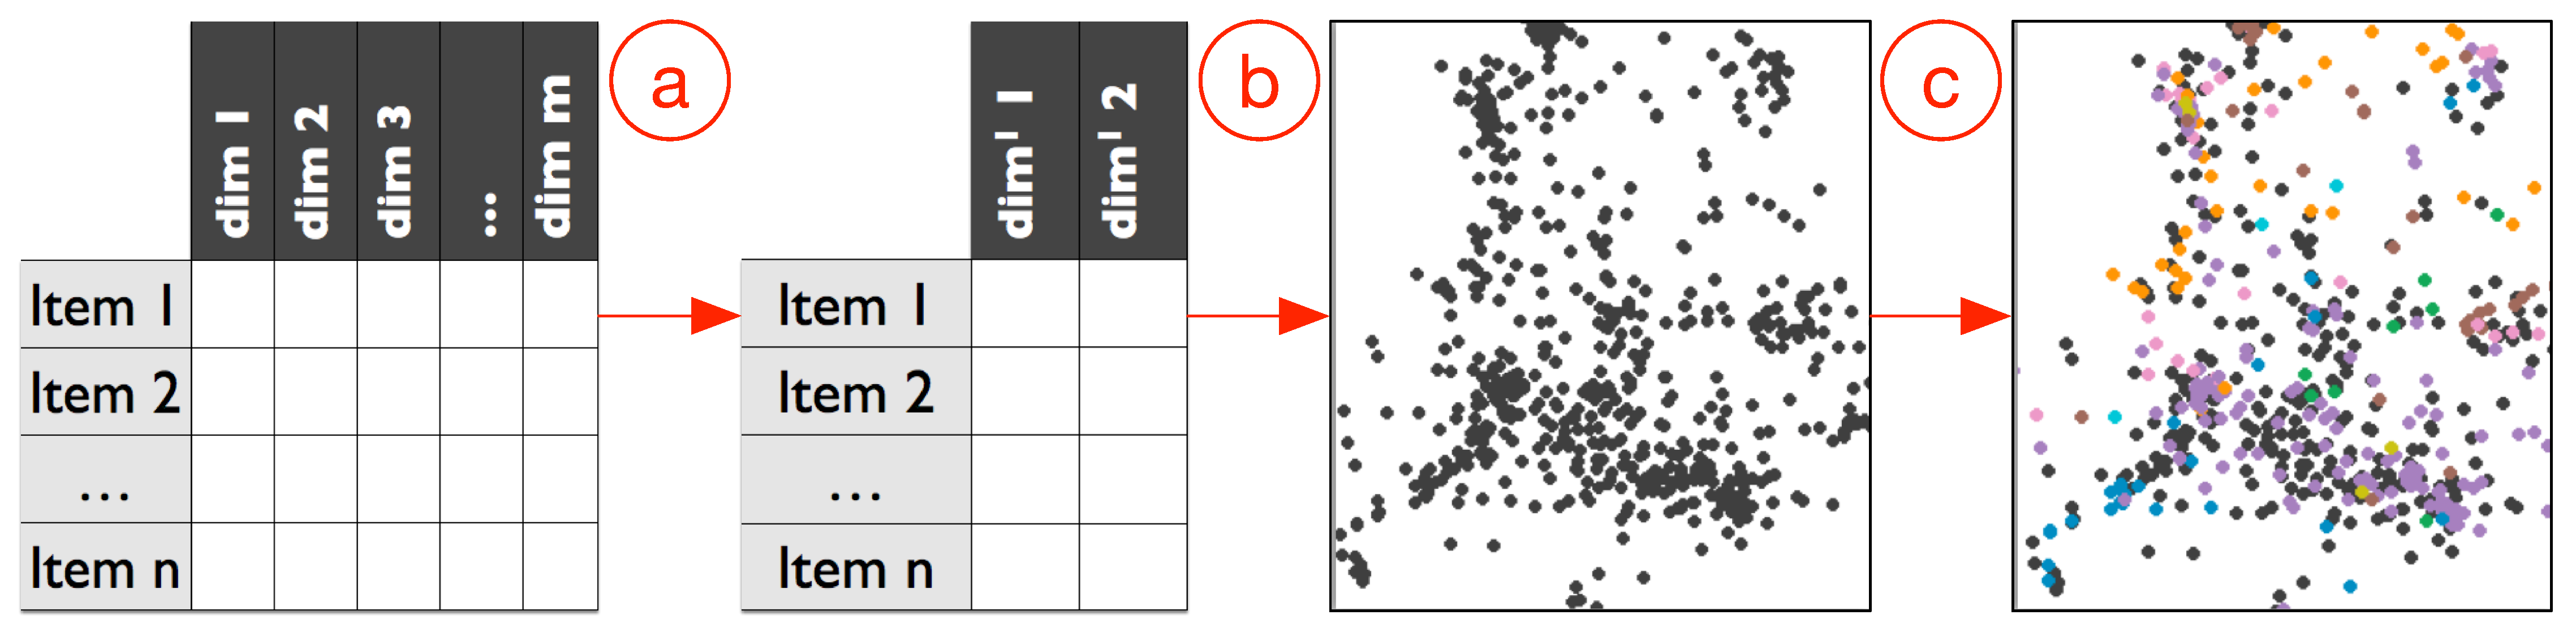
\includegraphics[width=\textwidth]{figures/drvizsequence.eps}
	\caption
	[
	    A task sequence involving dimensionally reduced data.
	]
	{
    	A task sequence involving dimensionally reduced data. (a) Data is reduced to two dimensions; (b) {\tt encoded} in a scatterplot to {\tt verify} visible clusters; and (c) colour-coded according to preexisting class labels to \textsl{match} clusters and classes.
	}
	\centering
	\label{drvistasks:fig:drvizsequence}
\end{figure} 

%-|-|-|-|-|-|-|-|-|-|-|-|-|-|-|-|-|-|-|-|-|-|-|-|-|-|-|-|-|-|-|-|-|-|-|-|-

The contribution of this chapter is a classification of five task sequences\index{task!task sequence} related to the visualization of dimensionally reduced\index{dimensionality reduction (DR)} data: {\it naming synthesized dimensions}, {\it mapping a synthesized dimension to original dimensions}, {\it verifying clusters}, {\it naming clusters}, and  {\it matching clusters and classes}. 
In the last of these sequences\index{task!task sequence}, illustrated in \autoref{drvistasks:fig:drvizsequence}, an analyst uses \ac{DR}\index{dimensionality reduction (DR)} and scatterplots\index{visual encoding!scatterplot} to verify\index{{\tt discover}} clusters, and then match them with existing classes.
Our classification is based on an in-depth analysis of ten interviews with analysts who use \ac{DR}\index{dimensionality reduction (DR)} for visualizing their data, as well as on a literature review of papers that apply \ac{DR}\index{dimensionality reduction (DR)} for the purpose of data visualization.
Our analysis\index{task!task analysis} framework is our typology\index{task!task typology} of abstract tasks\index{task!task abstraction} proposed in \autoref{ch:typology}.
Our typology\index{task!task typology} allows practitioners to characterize task sequences\index{task!task sequence} based on observed work practices\index{work domain analysis}, occurring in requirements gathering activities and in field evaluations\index{evaluation} of deployed tools.

%-------------------------------------------------------------------------
%-------------------------------------------------------------------------

\section{Related Work}
\label{drvistasks:rw}

%-------------------------------------------------------------------------
%-------------------------------------------------------------------------

\bstart{Classifying tasks}
The systematic analysis\index{task!task analysis} of worker activities\index{work domain analysis} and tasks\index{task} is a critical process in the design and evaluation\index{evaluation} of technology, and task analysis\index{task!task analysis} frameworks appear in many different fields, including human factors and ergonomics~\cite{Vicente1999}, \ac{HCI}\index{human-computer interaction (HCI)}~\cite{Mullins1993}, and visualization, including the typology\index{task!task typology} of tasks proposed in \autoref{ch:typology}.

While many classifications of visualization tasks\index{task} are agnostic to datatype, some address specific types of data~\cite{Shneiderman1996}, such as network data~\cite{Lee2006}, time-oriented data~\cite{Lammarsch2012}\index{time-oriented data}, and tabular data~\cite{Henry2006}.
As we discussed in \autoref{typology:rw:taxonomies} and in \citet{Meyer2015}, datatype-specific task\index{task} classifications consider a specific set of {\it data abstractions}\index{data abstraction}, facilitating a mapping to appropriate visual encoding\index{visual encoding} and interaction\index{interaction} design choices.
A datatype-specific task\index{task} classification of tasks\index{task} is also critical for evaluation\index{evaluation}, such as when specifying tasks\index{task} to be performed by participants in controlled experiments.
In this chapter, we propose a datatype-specific classification of task sequences\index{task!task sequence} for {\it dimensionally reduced}\index{dimensionality reduction (DR)} data. 

Classifications of tasks\index{task} are often based on their authors' own experience in conjunction with a thorough consideration of the literature~\cite{Amar2004,Shneiderman1996}, while others are based on observations of human behaviour in controlled laboratory settings~\cite{Amar2005}. 
In contrast, our classification of task sequences\index{task!task sequence} is primarily based on an interview study with analysts working with their own data~\cite{McGrath1995}, allowing us to ground our findings in real data analysis practices.

\begin{sloppypar}
\bstart{Mapping tasks to design choices for high-dimensional data analysis}
There are many approaches that combine analysis of high-dimensional data\index{high-dimensional data}, \ac{DR}\index{dimensionality reduction (DR)}, and visualization, including some developed by our research group~\cite{Ingram2010,Ingram2009,Williams2004}.
While there are existing classifications of high-dimensional data\index{high-dimensional data} analysis techniques~\cite{Bertini2011} and of dimensionally reduced\index{dimensionality reduction (DR)} data~\cite{Sedlmair2012a}, the mapping between data, tasks\index{task}, and appropriate design choices remains unclear~\cite{Tatu2010a}. 
This problem is particularly apparent when designing to accommodate {\it workflows}\index{workflows}, or instantiations of task sequences\index{task!task sequence} within software tools for high-dimensional data\index{high-dimensional data} analysis~\cite{Ingram2010,Johansson2009}.
\end{sloppypar}

One task\index{task} for dimensionally reduced\index{dimensionality reduction (DR)} data is that of matching clusters and categorical classes given with the data, discussed below in \autoref{drvistasks:tasks:clusters}. 
Based on findings from an empirical data study, we previously identified effective visual encoding design choices that support this task~\cite{Sedlmair2013}, and we called for similar work to be done for other tasks\index{task} relating to dimensionally reduced\index{dimensionality reduction (DR)} data.
Our classification of task sequences\index{task!task sequence} moves us closer to this goal.

\bstart{Expert judgments and dimensionally reduced\index{dimensionality reduction (DR)} data}
We are aware of one other study involving expert analysts' interpretations of visualized dimensionally reduced\index{dimensionality reduction (DR)} data, though they do not share our explicit examination of analysts' domain problems and tasks\index{task}: \citet{Lewis2012} asked expert and novice analysts in a controlled lab setting to subjectively rate the value of two-dimensional scatterplots\index{visual encoding!scatterplot} of seven dimensionally reduced\index{dimensionality reduction (DR)} datasets, generated using nine different \ac{DR}\index{dimensionality reduction (DR)} techniques. 
Their findings showed that experts were more consistent than novices in their positive and negative ratings.
Judging the value or quality of a visual encoding\index{visual encoding} of dimensionally reduced\index{dimensionality reduction (DR)} data should occur regardless of task\index{task}, and analysts can additionally leverage automated quality metrics based on human perception~\cite{Albuquerque2010a,Bertini2011}. 
In our study, the domain experts we interviewed varied in terms of their perceived understanding of \ac{DR}\index{dimensionality reduction (DR)}; furthermore, we sought to characterize experts' tasks\index{task} and activities in naturalistic settings, rather than in a controlled lab study.

%-------------------------------------------------------------------------
%-------------------------------------------------------------------------

\section{Research Process}
\label{drvistasks:methods}

%-------------------------------------------------------------------------
%-------------------------------------------------------------------------

Our methodological choice was motivated by a vibrant thread of work in the visualization community using qualitative methods in general~\cite{Carpendale2008,Isenberg2008,Tory2008}, and interview studies in particular~\cite{Kandel2012,Kang2011}\footnote{We elaborate on the evolution of our methodology and the foci of our analysis in \autoref{app:drvistasks:methodology}.}.

\bstart{Data collection}
Between 2010 and 2012, we interviewed nineteen data analysts working in academic and industry settings, representing over a dozen domains, spanning the natural sciences, computer science, policy analysis\index{policy analysis}, and investigative journalism\index{journalism}. 
These analysts were recruited from our extended personal and professional networks via snowball sampling, and they were known to work with high-dimensional data\index{high-dimensional data}.
These interviews were semi-structured, lasting in duration from one to four hours\footnote{In \autoref{app:drvistasks:interview-list}, we indicate that we conducted twenty-four interviews in total, as five analysts were interviewed twice; see \autoref{tab:interviews}.}; some of these interviews were more akin to contextual inquiries~\cite{Holtzblatt1993}\index{evaluation!contextual inquiry}, occurring at the analyst's workplace, while others were performed in our department or via teleconference.

We discussed the analysts' domain context, their data analysis goals, and their data; we also asked more specific questions about how they transformed their data and their use of \ac{DR}\index{dimensionality reduction (DR)} and visualization techniques\footnote{The interview foci and questions can be found in \autoref{app:drvistasks:interview-foci}}.
We also collected artifacts from these analysts, including their published papers and theses, their unpublished manuscripts, screenshots of their visualized data, and in some cases, even their data.

\bstart{Data analysis}
We alternated between data collection and analysis, progressing from {\it initial} to {\it focused} coding\index{coding (qualitative data analysis)} of the data~\cite{Charmaz2006}\footnote{Example artefacts from this data analysis process can be found in \autoref{app:drvistasks:analysis-examples}.}\index{grounded theory}.

In this chapter we concentrate our attention on the ten analysts who (a) specifically used dimensional synthesis \ac{DR}\index{dimensionality reduction (DR)!dimensional synthesis} algorithms\index{algorithms} in analyzing their high-dimensional data\index{high-dimensional data}, and who (b) also visualized their dimensionally reduced\index{dimensionality reduction (DR)} data.

To analyze the data that we collected from these ten interviews, we used our typology\index{task!task typology} of abstract visualization tasks\index{task!task abstraction}, proposed in \autoref{ch:typology}.
Our typology\index{task!task typology} distinguishes {\it why}\index{{\tt why}} data is being visualized at multiple levels of abstraction\index{task!task abstraction}, {\it what}\index{{\tt what}} {\tt inputs}\index{{\tt input}} and {\tt outputs}\index{{\tt output}} a task\index{task} may have, as well as {\it how}\index{{\tt how}} a task\index{task} is supported by visual encoding\index{visual encoding} and interaction\index{interaction} design choices. 
This lens allowed us to focus on a subset of our findings from the standpoint of visualization design and evaluation\footnote{The previous interpretations of our findings are documented in \autoref{app:drvistasks:previous-interpretations}. We initially focused on characterizing \ac{DR}\index{dimensionality reduction (DR)} techniques, people who use them, their tasks\index{task}, and their challenges~\cite{Sedlmair2012b}. 
Later, we narrowed our focus to that of \ac{DR}\index{dimensionality reduction (DR)} techniques and related tasks\index{task} (see \autoref{app:drvistasks:dritw}). 
In this chapter, our focus is even narrower, on tasks\index{task} relating to the visualization of dimensionally reduced data following the use of dimensional synthesis \ac{DR} techniques.}\index{evaluation}, culminating in the task sequences\index{task!task sequence} presented in \autoref{drvistasks:tasks}.
In Section \ref{drvistasks:typology}, we revisit the typology\index{task!task typology} and illustrate how it can describe our five task sequences\index{task!task sequence}. 
%RR: p. 51, bottom. Using the typology to "better interpret" the data. Although any reference frame causes some things to be emphasized (and thus, better interpreted), it also causes others to be de-emphasized, or even lost. What's lost here? More generally, what are the weakest aspects of this approach? Could they be fixed, given enough time?

Finally, we enriched our analysis with further examples from the literature.
We specifically sought papers that report on applications where \ac{DR}\index{dimensionality reduction (DR)} and visualization were performed in conjunction for analysis, and we consider these applications with respect to the task sequences\index{task!task sequence} we characterized. 

%-------------------------------------------------------------------------
%-------------------------------------------------------------------------

\section{Task Sequences}
\label{drvistasks:tasks}

%-------------------------------------------------------------------------
%-------------------------------------------------------------------------

%-|-|-|-|-|-|-|-|-|-|-|-|-|-|-|-|-|-|-|-|-|-|-|-|-|-|-|-|-|-|-|-|-|-|-|-|-

\begin{figure}
	\centering
	\begin{subfigure}[t]{\textwidth}
	    \centering
        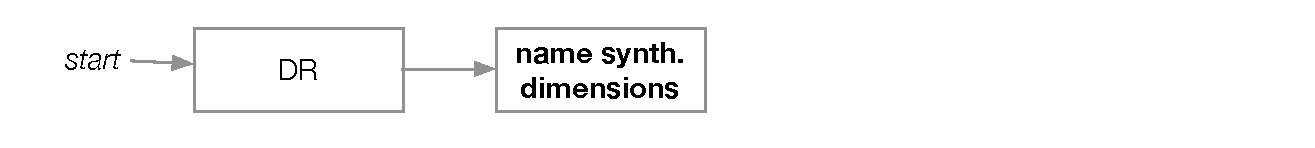
\includegraphics[height=1cm]{figures/drviztasks-name-dims.eps}
    \end{subfigure}
    ~
    \begin{subfigure}[t]{\textwidth}
	    \centering
        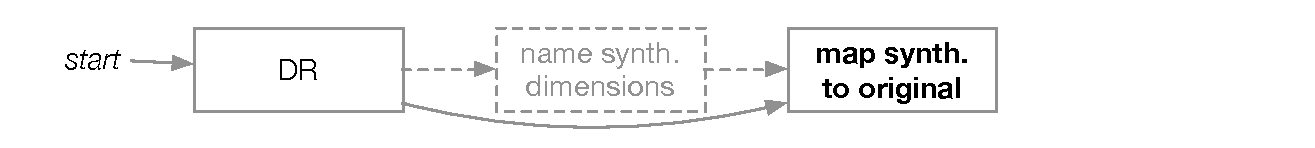
\includegraphics[height=1cm]{figures/drviztasks-map-dims.eps}
    \end{subfigure}
    ~
    \begin{subfigure}[t]{\textwidth}
	    \centering
        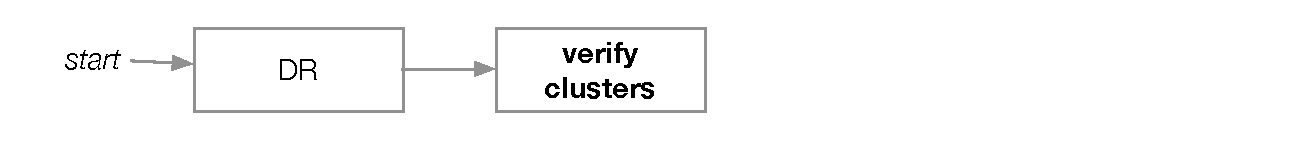
\includegraphics[height=1cm]{figures/drviztasks-identify-clusters.eps}
    \end{subfigure}
    ~
    \begin{subfigure}[t]{\textwidth}
	    \centering
        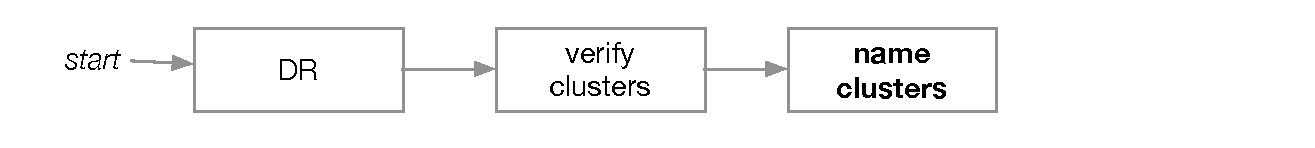
\includegraphics[height=1cm]{figures/drviztasks-name-clusters.eps}
    \end{subfigure}
    ~
    \begin{subfigure}[t]{\textwidth}
	    \centering
        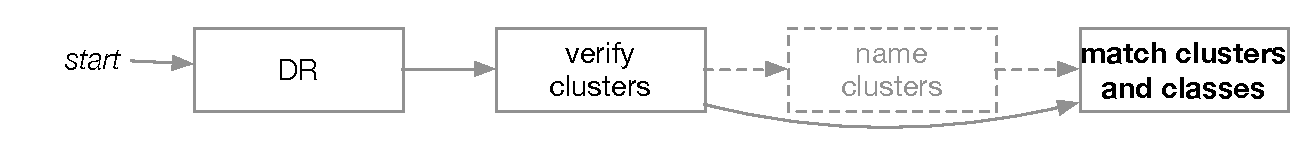
\includegraphics[height=1cm]{figures/drviztasks-match-clusters.eps}
    \end{subfigure}
	\caption
	[
	    Five task sequences that involve visualizing dimensionally reduced data.
	]
	{
    	
    	Five task sequences that involve visualizing dimensionally reduced data. Individual tasks are described using our typology in \autoref{drvistasks:fig:drviztasks}.
	}
	\centering
	\label{drvistasks:sequences}
\end{figure}

%-|-|-|-|-|-|-|-|-|-|-|-|-|-|-|-|-|-|-|-|-|-|-|-|-|-|-|-|-|-|-|-|-|-|-|-|-

We have identified five task sequences\index{task!task sequence} related to dimensionally reduced\index{dimensionality reduction (DR)} data.
In this section, we describe each task sequence\index{task!task sequence} and illustrate the sequence\index{task!task sequence} in \autoref{drvistasks:sequences}. 
Each is named after the terminal task\index{task} appearing in the sequence\index{task!task sequence}.
We also comment on how these task sequences\index{task!task sequence} arose in our interviews, and which visualization techniques were used to address these sequences\index{task!task sequence}. 
These task sequences\index{task!task sequence} are not exclusive: some analysts performed multiple task sequences\index{task!task sequence} in the course of their work.
This descriptive survey of analysts' data, task sequences\index{task!task sequence}, and visualization is summarized in \autoref{drvistasks:tab:summary}. 
The dataset sizes being investigated by these analysts ranged from dozens to over a million dimensions, and from hundreds to hundreds of thousands of items.  

%-|-|-|-|-|-|-|-|-|-|-|-|-|-|-|-|-|-|-|-|-|-|-|-|-|-|-|-|-|-|-|-|-|-|-|-|-

\begin{table}\renewcommand{\arraystretch}{1.2}\addtolength{\tabcolsep}{-1pt}
	\begin{center}
	\tiny
	\begin{tabular}{@{}|l|>{\RaggedRight}p{0.125\textwidth}l|*{2}c|*{5}c|*{7}c|@{}}

		\hline

		\cellcolor{blue!15} {\bf Case}
		& \multicolumn{2}{c|}{\cellcolor{blue!15} {\bf Data}} 
		& \multicolumn{2}{c|}{\cellcolor{blue!15} {\bf DR}} 
		& \multicolumn{5}{c|}{\cellcolor{blue!15} {\bf Task Sequence}} 
		& \multicolumn{7}{c|}{\cellcolor{blue!15} {\bf Visualization Techniques}}

		\\

		\hline

		\rowcolor{blue!15}

		{\rot{\bf ID}}

		& {\rot{\bf Description}} & {\rot{\bf \# Dims x Items}}

		& {\rot{\bf Linear}} & {\rot{\bf Non-Linear}}

		& {\rot{\it Name Dimensions}} & {\rot{\it Map Dimensions}} & {\rot{\it Verify Clusters}} & {\rot{\it Name Clusters}} & {\rot{\it Match Clusters}}

		& {\rot{\bf 2D Scatterplots}\index{visual encoding!scatterplot}} & {\rot{\bf 3D Scatterplots}\index{visual encoding!scatterplot!3D scatterplot}} & {\rot{\bf SPLOMs}}\index{visual encoding!scatterplot!scatterplot matrix (SPLOM)} & {\rot{\bf Scree plots}\index{visual encoding!scree plot}} & {\rot{\bf Graph / Tree}}\index{visual encoding!tree}\index{visual encoding!node-link graph} & {\rot{\bf Correl. matrix}}\index{visual encoding!matrix!correlation matrix} & {\rot{\bf Heat maps}\index{visual encoding!heat map}}

		\\

		\hline

		\refstepcounter{rownumber} 
		\therownumber\label{drvistasks:analyst:JB} %Music / Jennifer Büttgen

% 		& HCI

		& usage logs from online music service & 48 x 310 %10\textsuperscript{1} &  10\textsuperscript{2} %48, 310

		& \OK & 

		& \OK & \OK & \OK & \OK & \OK 
		%[i] \ac{DR}\textsuperscript{1} $\rightarrow$ {\it name synth. dims} $\rightarrow$ {\it map synth. to original }; [ii] \ac{DR}\textsuperscript{1} $\rightarrow$ {\it verify clusters} $\rightarrow$ {\it name clusters} $\rightarrow$ {\it match clusters and classes}

		& \OK & & \OK & & & & 
		%2D scatterplots, \ac{SPLOM}s

		\\

		\rowcolor{gray!15}

		\refstepcounter{rownumber} 
		\therownumber\label{drvistasks:analyst:HL} %Search / Heidi Lam

% 		& HCI

		& aggregated search engine metrics  & 12--31 x 1,463%10\textsuperscript{1} & 10\textsuperscript{3} % 12-31,1463

		& \OK & \OK 

		& \OK & \OK & \OK & \OK & \OK 
		%[i] \ac{DR}\textsuperscript{1,2} $\rightarrow$ {\it name synth. dims} $\rightarrow$ {\it map synth. to original }; [ii] \ac{DR}\textsuperscript{1,2} $\rightarrow$ {\it verify clusters} $\rightarrow$ {\it name clusters} $\rightarrow$ {\it match clusters and classes}

		& \OK & & & & & & 
		%2D scatterplots

		\\

		\refstepcounter{rownumber} 
		\therownumber\label{drvistasks:analyst:CM} %BoatAct / Cindy Marven

% 		& PA

		& recreational boating survey data & 39 x 543 %10\textsuperscript{1} & 10\textsuperscript{2} %39, 543

		& \OK & \OK

		& & \OK & \OK & \OK &
		%[i] \ac{DR}\textsuperscript{1,2} $\rightarrow$ {\it map synth. to original }; [ii] \ac{DR}\textsuperscript{1,2} $\rightarrow$ {\it verify clusters} $\rightarrow$ {\it name clusters}

		& \OK & \OK & \OK & & \OK & & 
		% 2D scatterplots, 3D scatterplots, \ac{SPLOM}s, dendrograms

		\\ 

		\rowcolor{gray!15}

		\refstepcounter{rownumber} 
		\therownumber\label{drvistasks:analyst:CN} %EpiGen / Cydney Nielsen

% 		& BI

		& protein region data & 160 x 10--100K%10\textsuperscript{2} & 10\textsuperscript{5} % 160, 10-100k

		& \OK & \OK

		& & \OK & \OK & \OK &  
		%[i] \ac{DR}\textsuperscript{1,2} $\rightarrow$ {\it map synth. to original }; [ii] \ac{DR}\textsuperscript{1,2} $\rightarrow$ {\it verify clusters} $\rightarrow$ {\it name clusters}

		& & & \OK & & & & \OK %, {\it Spark}~\cite{Nielsen2012}
		% \ac{SPLOM}s, density plots, heatmaps %, {\it Spark}~\cite{Nielsen2012}

		\\

		\refstepcounter{rownumber} 
		\therownumber\label{drvistasks:analyst:ST} %Polymers / Sid Thakur

% 		& CH

		& polymer molecule feature vectors & 1K x 10K %10\textsuperscript{3} & 10\textsuperscript{4} % 1k,10k

		& \OK & \OK

		& & & \OK & \OK & 
		
		% \ac{DR}\textsuperscript{1,2} $\rightarrow$ {\it verify clusters} $\rightarrow$ {\it name clusters}

		& \OK & & & & & \OK & \OK
		% 2D scatterplots, heatmaps, correlation matrices

		\\

		\rowcolor{gray!15}

		\refstepcounter{rownumber} 
		\therownumber\label{drvistasks:analyst:HY} %Concept / Hong Yi

% 		& SN

		& bibliometric co-occurrence matrix & 20K x 20K %10\textsuperscript{4} & 10\textsuperscript{4} % 20k

		& \OK & \OK

		& & & \OK & \OK &
		%1. \ac{DR}\textsuperscript{1,2} $\rightarrow$ {\it name synth. dims}; 2. 
		%\ac{DR}\textsuperscript{1,2} $\rightarrow$ {\it verify clusters} $\rightarrow$ {\it name clusters}

		& \OK & & \OK & \OK & & \OK &
		% 2D scatterplots, {\it DimStiller}~\cite{Ingram2010} (\ac{SPLOM}s, correlation matrices)

		\\

		\refstepcounter{rownumber} 
		\therownumber\label{drvistasks:analyst:KA} %MoCap / Kerem Altun

% 		& HCI 

		& human motions from multiple sensors & 1,170 x 9,120 %10\textsuperscript{3} & 10\textsuperscript{3} %1170, 9120

		& \OK & 

		& & & \OK & & \OK  
		%\ac{DR}\textsuperscript{1} $\rightarrow$ {\it verify clusters} $\rightarrow$ {\it match clusters and classes}

		& \OK & \OK & & & & &
		% 2D scatterplots, interactive 3D scatterplots

		\\

		\rowcolor{gray!15}

		% H %ChemRel / Klaus Dress

		% & Computational chemistry

		% & \ac{DR}\textsuperscript{2} $\rightarrow$ {\it verify clusters} $\rightarrow$ {\it match clusters and classes}

		% % & non-linear

		% & correlation matrices, {\it Spotfire}~\cite{Spotfire}, {\it Tableau}~\cite{Tableau}

		% \\

		\refstepcounter{rownumber} 
		\therownumber\label{drvistasks:analyst:AC} %ProstCan / Anamaria Crisan

% 		& BI

		& genomic, clinical data from patients & 1.4M x 600 %10\textsuperscript{6} & 10\textsuperscript{2} %1.4M, 600

		& \OK & \OK

		& & & \OK & & \OK
		%\ac{DR}\textsuperscript{1,2} $\rightarrow$ {\it verify clusters} $\rightarrow$ {\it match clusters and classes}

		& \OK & \OK & & & & &
		% 2D scatterplots, 3D scatterplots

		\\

		\refstepcounter{rownumber} 
		\therownumber\label{drvistasks:analyst:DH} %SeqAln / Des Higgins

% 		& BI

		& distance matrix of genome sequences & 100K x 100K %10\textsuperscript{5} & 10\textsuperscript{5} %100k

		& \OK & \OK

		& & & \OK & \OK & \OK
		%\ac{DR}\textsuperscript{1,2} $\rightarrow$ {\it verify clusters} $\rightarrow$ {\it name clusters} $\rightarrow$ {\it match clusters and classes}

		& \OK & \OK & \OK & & \OK & &
		% 2D scatterplots, 3D scatterplots, \ac{SPLOM}s, node-link graphs

		\\

		\rowcolor{gray!15}

		\refstepcounter{rownumber} 
		\therownumber\label{drvistasks:analyst:JS} %TxtDocs / Jonathan Stray

% 		& IJ

		& distance matrix of text documents & 10K x 10K %10\textsuperscript{4} & 10\textsuperscript{4} %10k

		&  & \OK

		& & & \OK & \OK & \OK
		%\ac{DR}\textsuperscript{2} $\rightarrow$ {\it verify clusters} $\rightarrow$ {\it name clusters} $\rightarrow$ {\it match clusters and classes}

		& \OK & & & & \OK & &
		% 2D scatterplots, node-link graphs

		\\

		\hline

		\rowcolor{blue!15}

		{\bf Ref.}

% 		& 

		& 

		& %dims	
% 		& %items

		& %linear 
		& %non-linear

		& %name dims
		& %map dims
		& %verify clusters
		& %name clusters
		& %match clusters

		& %2D SPs
		& %3D SPs
		& %\ac{SPLOM}s
		& %scree plots
		& %node-link
		& %correl matrix
		& %heatmaps

		\\

		\hline

		\cite{Buja2002} %MorseCd
% 		\cite{Tenenbaum2000} %Faces
% 		\cite{Matusik2003} %BRDF
% 		\cite{Reveret2005} %Quadrup

% 		& 

		& distance matrix of Morse codes & 36 x 36 %10\textsuperscript{1} & 10\textsuperscript{1} %26

		& & \OK

		% & linear; non-linear

		&  \OK &  & \OK  & \OK  & 

		% \ac{DR}\textsuperscript{1,2} $\rightarrow$ {\it name synth. dims}

		&  \OK &  &  & & & &

		% 2D scatterplots with text labels and inter-class connections 

		\\

		\rowcolor{gray!15}

		\cite{Matusik2003} %BRDF

% 		& 

		& BRDF reflectance model & 4.36M x 104 %10\textsuperscript{6} & 10\textsuperscript{2} %4364000, 104

		& \OK & \OK 

		% & linear; non-linear

		&  \OK &  &  &  & 

		% \ac{DR}\textsuperscript{1,2} $\rightarrow$ {\it name synth. dims}

		& \OK &  &  & \OK & & &

		% 2D scatterplots with text labels 

		\\

		\cite{Reveret2005} %Quadrup

% 		& 

		& quadruped skeleton models & 348--406 x 9 %10\textsuperscript{2} & 10\textsuperscript{1} %348-406, 9

		& \OK &
		%linear

		& \OK & & & &
		% \ac{DR}\textsuperscript{1} $\rightarrow$ {\it name synth. dims}

		% & linear

		& & & & \OK & & &
		% Scree plot

		\\

		\rowcolor{gray!15}

		\cite{Tenenbaum2000} %Faces

% 		& 

		& 64 x 64 px images & 4,096 x 698--1K %10\textsuperscript{3} & 10\textsuperscript{2} %4096, 698-1000

		& & \OK
		% non-linear

		& \OK & & & &
		% \ac{DR}\textsuperscript{2} $\rightarrow$ {\it name synth. dims}

		& \OK & & & \OK & & &
		% 2D scatterplots with image glyphs adjacent to points

		\\

		% \cite{Bronstein2006a} %ArtShp

		% & Computer graphics

		% & \ac{DR}\textsuperscript{2} $\rightarrow$ {\it verify clusters} $\rightarrow$ {\it match clusters and classes}

		% % & non-linear

		% & similarity matrix

		% \\

		\hline

	\end{tabular}
	\caption
	[
	    A summary of task sequences performed by the ten analysts that we interviewed and found in papers discussing \ac{DR} and visualization.
	]
	{
	    {\it Top}: A summary of task sequences performed by the ten analysts that we interviewed, along with the visualization techniques(s) used to perform these tasks sequences. 
	   % *Domains: HCI = Human-Computer Interaction; PA = Policy Analysis; BI = Bioinformatics; CH = Chemistry; SN = Social Network Analysis; IJ = Investigative Journalism. 
	    {\it Bottom}: examples of task sequences in papers discussing \ac{DR} and visualization.
	} 
	\label{drvistasks:tab:summary}
	\end{center}
\end{table}

%-|-|-|-|-|-|-|-|-|-|-|-|-|-|-|-|-|-|-|-|-|-|-|-|-|-|-|-|-|-|-|-|-|-|-|-|-

\bstart{Dimensionality reduction}
All the task sequences\index{task!task sequence} we characterized begin with \ac{DR}\index{dimensionality reduction (DR)}.
In our context, we define \ac{DR}\index{dimensionality reduction (DR)} as a means\index{task!means} of dimensional synthesis\index{dimensionality reduction (DR)!dimensional synthesis}: a set of $m$ synthesized dimensions is {\tt derived}\index{{\tt derive}} from $n$ original dimensions, where $m$~\textless~$n$. 
Dimensional synthesis\index{dimensionality reduction (DR)!dimensional synthesis} techniques are commonly differentiated between {\it linear} and {\it non-linear}~\cite{Jain2000}. 
Linear techniques such as \ac{PCA}\index{dimensionality reduction (DR)!principal component analysis (PCA)}~\cite{Jolliffe2002} or classical \ac{MDS}\index{dimensionality reduction (DR)!multi-dimensional scaling (MDS)}~\cite{Torgerson1952,Young1938} produce\index{{\tt produce}} synthetic dimensions from linear projections of the original data. 
However, many datasets have an intrinsic structure that can only be revealed using non-linear techniques, such as Isomap~\cite{Tenenbaum2000}, \ac{t-SNE}\index{dimensionality reduction (DR)!t-distributed stochastic neighbor embedding (t-SNE)}~\cite{VanderMaaten2008}, or Glimmer \ac{MDS}\index{dimensionality reduction (DR)!multi-dimensional scaling (MDS)}~\cite{Ingram2009}.
Further distinction between linear and non-linear dimensional synthesis\index{dimensionality reduction (DR)!dimensional synthesis} is outside of the scope of this chapter, though we note that some techniques are more appropriate for verifying the existence of local cluster structure while others are more appropriate for identifying\index{{\tt identify}} global intrinsic dimensions (or {\it manifolds})~\cite{Lewis2012}.
In \autoref{drvistasks:tab:summary}, we note who used linear and non-linear \ac{DR}\index{dimensionality reduction (DR)}.

It is not our intent to catalog and differentiate the large body of \ac{DR}\index{dimensionality reduction (DR)} techniques; we will concentrate our analysis on their {\tt output}\index{{\tt output}}, asking {\it why}\index{{\tt why}} do analysts visualize these synthesized dimensions.

%-------------------------------------------------------------------------

\subsection{Dimension-Oriented Task Sequences}
\label{drvistasks:tasks:dims}

%-------------------------------------------------------------------------

We describe two task sequences\index{task!task sequence} that specifically relate to {\it synthesized} dimensions as generated by dimensional synthesis\index{dimensionality reduction (DR)!dimensional synthesis} \ac{DR}\index{dimensionality reduction (DR)} techniques: {\it naming synthesized dimensions} and {\it mapping synthesized to original dimensions}.
The verbs {\it name} and {\it map} were deliberately chosen and are defined using the vocabulary of our typology\index{task!task typology} in the following two subsections.

% %-------------------------------------------------------------------------

% \subsubsection{Name Synthesized Dimensions}
% \label{drvistasks:tasks:name-dims}

% %-------------------------------------------------------------------------

% \begin{figure}[!ht]
% 	\centering
% 	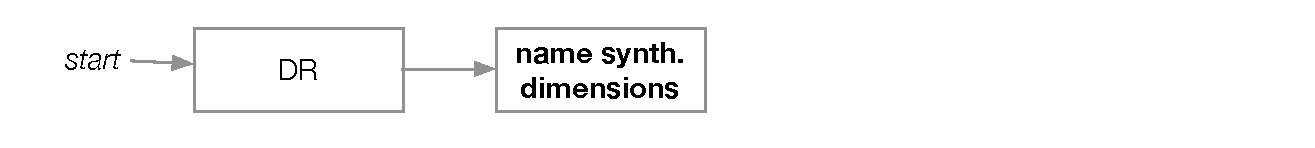
\includegraphics[width=\textwidth]{figures/drviztasks-name-dims.eps}
% 	\centering
% \end{figure} 

\bstart{Name synthesized dimensions}
Given a set of synthesized dimensions, an analyst may want to {\tt discover}\index{{\tt discover}} what these dimensions mean, to {\tt generate hypotheses}\index{{\tt discover}} about the semantics of these synthesized dimensions.
An analyst will {\tt browse}\index{{\tt browse}} the set of synthesized dimensions, and for each dimension of interest, she will {\tt browse}\index{{\tt browse}} items and their corresponding values; as a result, she may be able to {\tt identify}\index{{\tt identify}} the name of a synthesized dimension.

This task sequence\index{task!task sequence} was attempted by two of the analysts we interviewed (\ref{drvistasks:analyst:JB} and~\ref{drvistasks:analyst:HL} in \autoref{drvistasks:tab:summary}). 
Both worked in the field of \ac{HCI}\index{human-computer interaction (HCI)} and attempted to {\tt identify}\index{{\tt identify}} the intrinsic dimensions related to usage data collected about online search behaviour and music listening behaviour, respectively. 

A common approach, employed by both analysts, is to inspect data points plotted according to two synthesized dimensions in a two-dimensional scatterplot\index{visual encoding!scatterplot}, in which the analyst may be able to discern an interesting semantic relationship along the axes. 
In some cases, these scatterplots\index{visual encoding!scatterplot} are augmented with text labels containing categorical information, such as item name, annotated\index{{\tt annotate}} adjacent to a subset of the plotted points~\cite{Buja2002,Matusik2003,Tenenbaum2000} or available through interaction\index{interaction}. 
Tenenbaum~\etal's paper describing the Isomap algorithm~\cite{Tenenbaum2000} contains a particularly compelling example (reproduced in \autoref{drvistasks:fig:drviztasks-name-dims-tenenbaum}), in which each data point in a scatterplot\index{visual encoding!scatterplot} corresponds to an image of a face; a random sample of these images are displayed directly in the scatterplot\index{visual encoding!scatterplot} as thumbnails adjacent to their corresponding points.
Given this display, it is possible to discern names for the three synthesized dimensions resulting from dimensional synthesis\index{dimensionality reduction (DR)!dimensional synthesis}. 

\begin{figure}
	\centering
	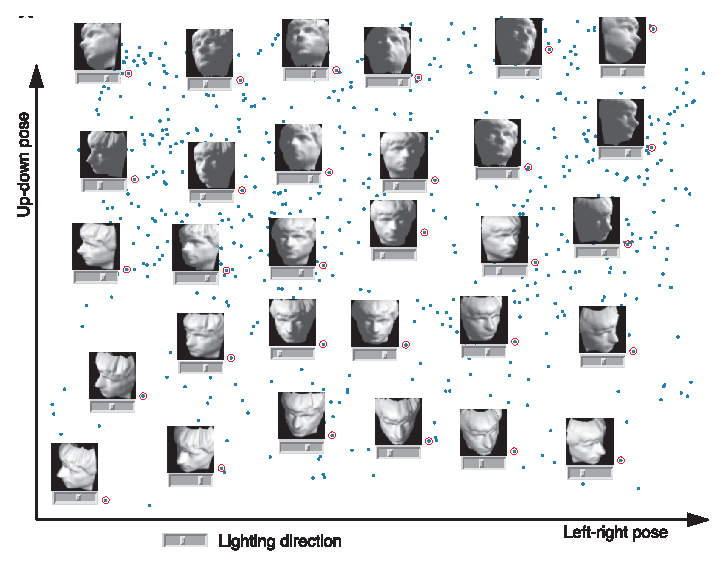
\includegraphics[width=\textwidth]{figures/drviztasks-name-dims-tenenbaum.eps}
	\caption
	[
	    A visual encoding of dimensionally reduced data, in which three synthesized dimensions have been identified.
	]
	{
    	 A visual encoding of dimensionally reduced data, in which three synthesized dimensions have been identified: \textsl{up-down pose} along the y-axis, \textsl{left-right pose} along the x-axis, and \textsl{lighting direction} indicated below each image.
    	 Figure from \citet{Tenenbaum2000} (\copyright~[2000] AAAS).
	}
	\centering
	\label{drvistasks:fig:drviztasks-name-dims-tenenbaum}
\end{figure} 

% %-------------------------------------------------------------------------

% \subsubsection{Map Synthesized to Original Dimensions}
% \label{drvistasks:tasks:map-dims}

% %-------------------------------------------------------------------------

% \begin{figure}[!ht]
% 	\centering
% 	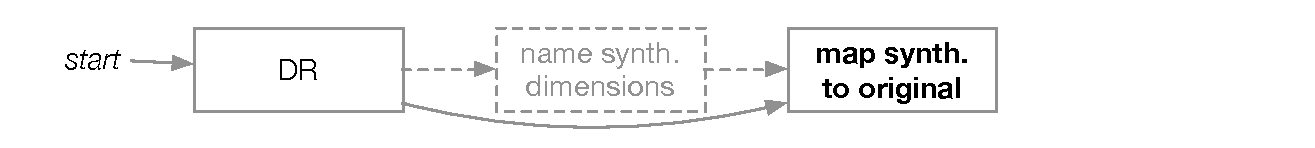
\includegraphics[width=\textwidth]{figures/drviztasks-map-dims.eps}
% 	\centering
% \end{figure} 

\bstart{Map synthesized to original dimensions}
Regardless of whether an analyst is interested in naming synthesized dimensions, another possible task sequence\index{task!task sequence} involves mapping synthesized dimensions back to original dimensions.
In the context of \ac{PCA}\index{dimensionality reduction (DR)!principal component analysis (PCA)}~\cite{Jolliffe2002}, this mapping is often referred to as the {\it loading} of the synthesized dimensions by the original dimensions.
Given a synthesized dimension, an analyst may want to {\tt discover}\index{{\tt discover}} this mapping. 
More specifically, the analyst may either {\tt verify}\index{{\tt discover}} a hypothesis that this mapping exists, or {\tt generate}\index{{\tt discover}} a new hypothesis about it. 
The analyst will {\tt browse}\index{{\tt browse}} items and their values along this synthesized dimension and {\tt compare}\index{{\tt compare}} these values to those along the set of original dimensions, looking for similarities and correlations.
This mapping could allow analysts to {\tt identify}\index{{\tt identify}} groups of correlated original dimensions.

Four of the analysts we interviewed attempted to perform this sequence\index{task!task sequence} of tasks; two of these analysts had previously attempted to name some of their synthesized dimensions.
\ref{drvistasks:analyst:JB} mapped her synthesized dimensions to a set of original dimensions in aggregated usage logs from an online music streaming service, while~\ref{drvistasks:analyst:HL} attempted the same task sequence\index{task!task sequence} with aggregate search engine metrics but was unable to confidently map any of her synthesized dimensions to her original dimensions. 
Both used two-dimensional scatterplots\index{visual encoding!scatterplot} to carry out this task sequence\index{task!task sequence}. 
The other two analysts were explicitly interested in grouping original dimensions based on this mapping: a policy analyst\index{policy analysis} (\ref{drvistasks:analyst:CM}) investigating survey data pertaining to recreational boating practices used two-dimensional scatterplots\index{visual encoding!scatterplot} to {\tt compare}\index{{\tt compare}} synthesized dimensions and original dimensions, while a bioinformatician\index{bioinformatics} (\ref{drvistasks:analyst:CN}) investigating protein regions used a \ac{SPLOM}\index{visual encoding!scatterplot!scatterplot matrix (SPLOM)}, heat maps\index{visual encoding!heat map}, and density plots\index{visual encoding!density plot}.

%-------------------------------------------------------------------------

\subsection{Cluster-Oriented Task Sequences}
\label{drvistasks:tasks:clusters}

%-------------------------------------------------------------------------

There exists another set of task sequences\index{task!task sequence} where the semantics of the synthesized dimensions are not a central interest; instead, analysts are interested in clusters of items that might be revealed in the dimensionally reduced\index{dimensionality reduction (DR)} data. 
We characterize three task sequences\index{task!task sequence}: 
{\it verify clusters}, {\it name clusters}, and {\it match clusters and classes}.
As with the dimension-oriented task sequences\index{task!task sequence}, the verbs {\it verify}, {\it name}, and {\it match} were deliberately chosen and are defined using the vocabulary of our typology\index{task!task typology} in the following three subsections.

%-|-|-|-|-|-|-|-|-|-|-|-|-|-|-|-|-|-|-|-|-|-|-|-|-|-|-|-|-|-|-|-|-|-|-|-|-

\begin{figure}
	\centering
	\begin{subfigure}[t]{0.45\textwidth}
	    \centering
        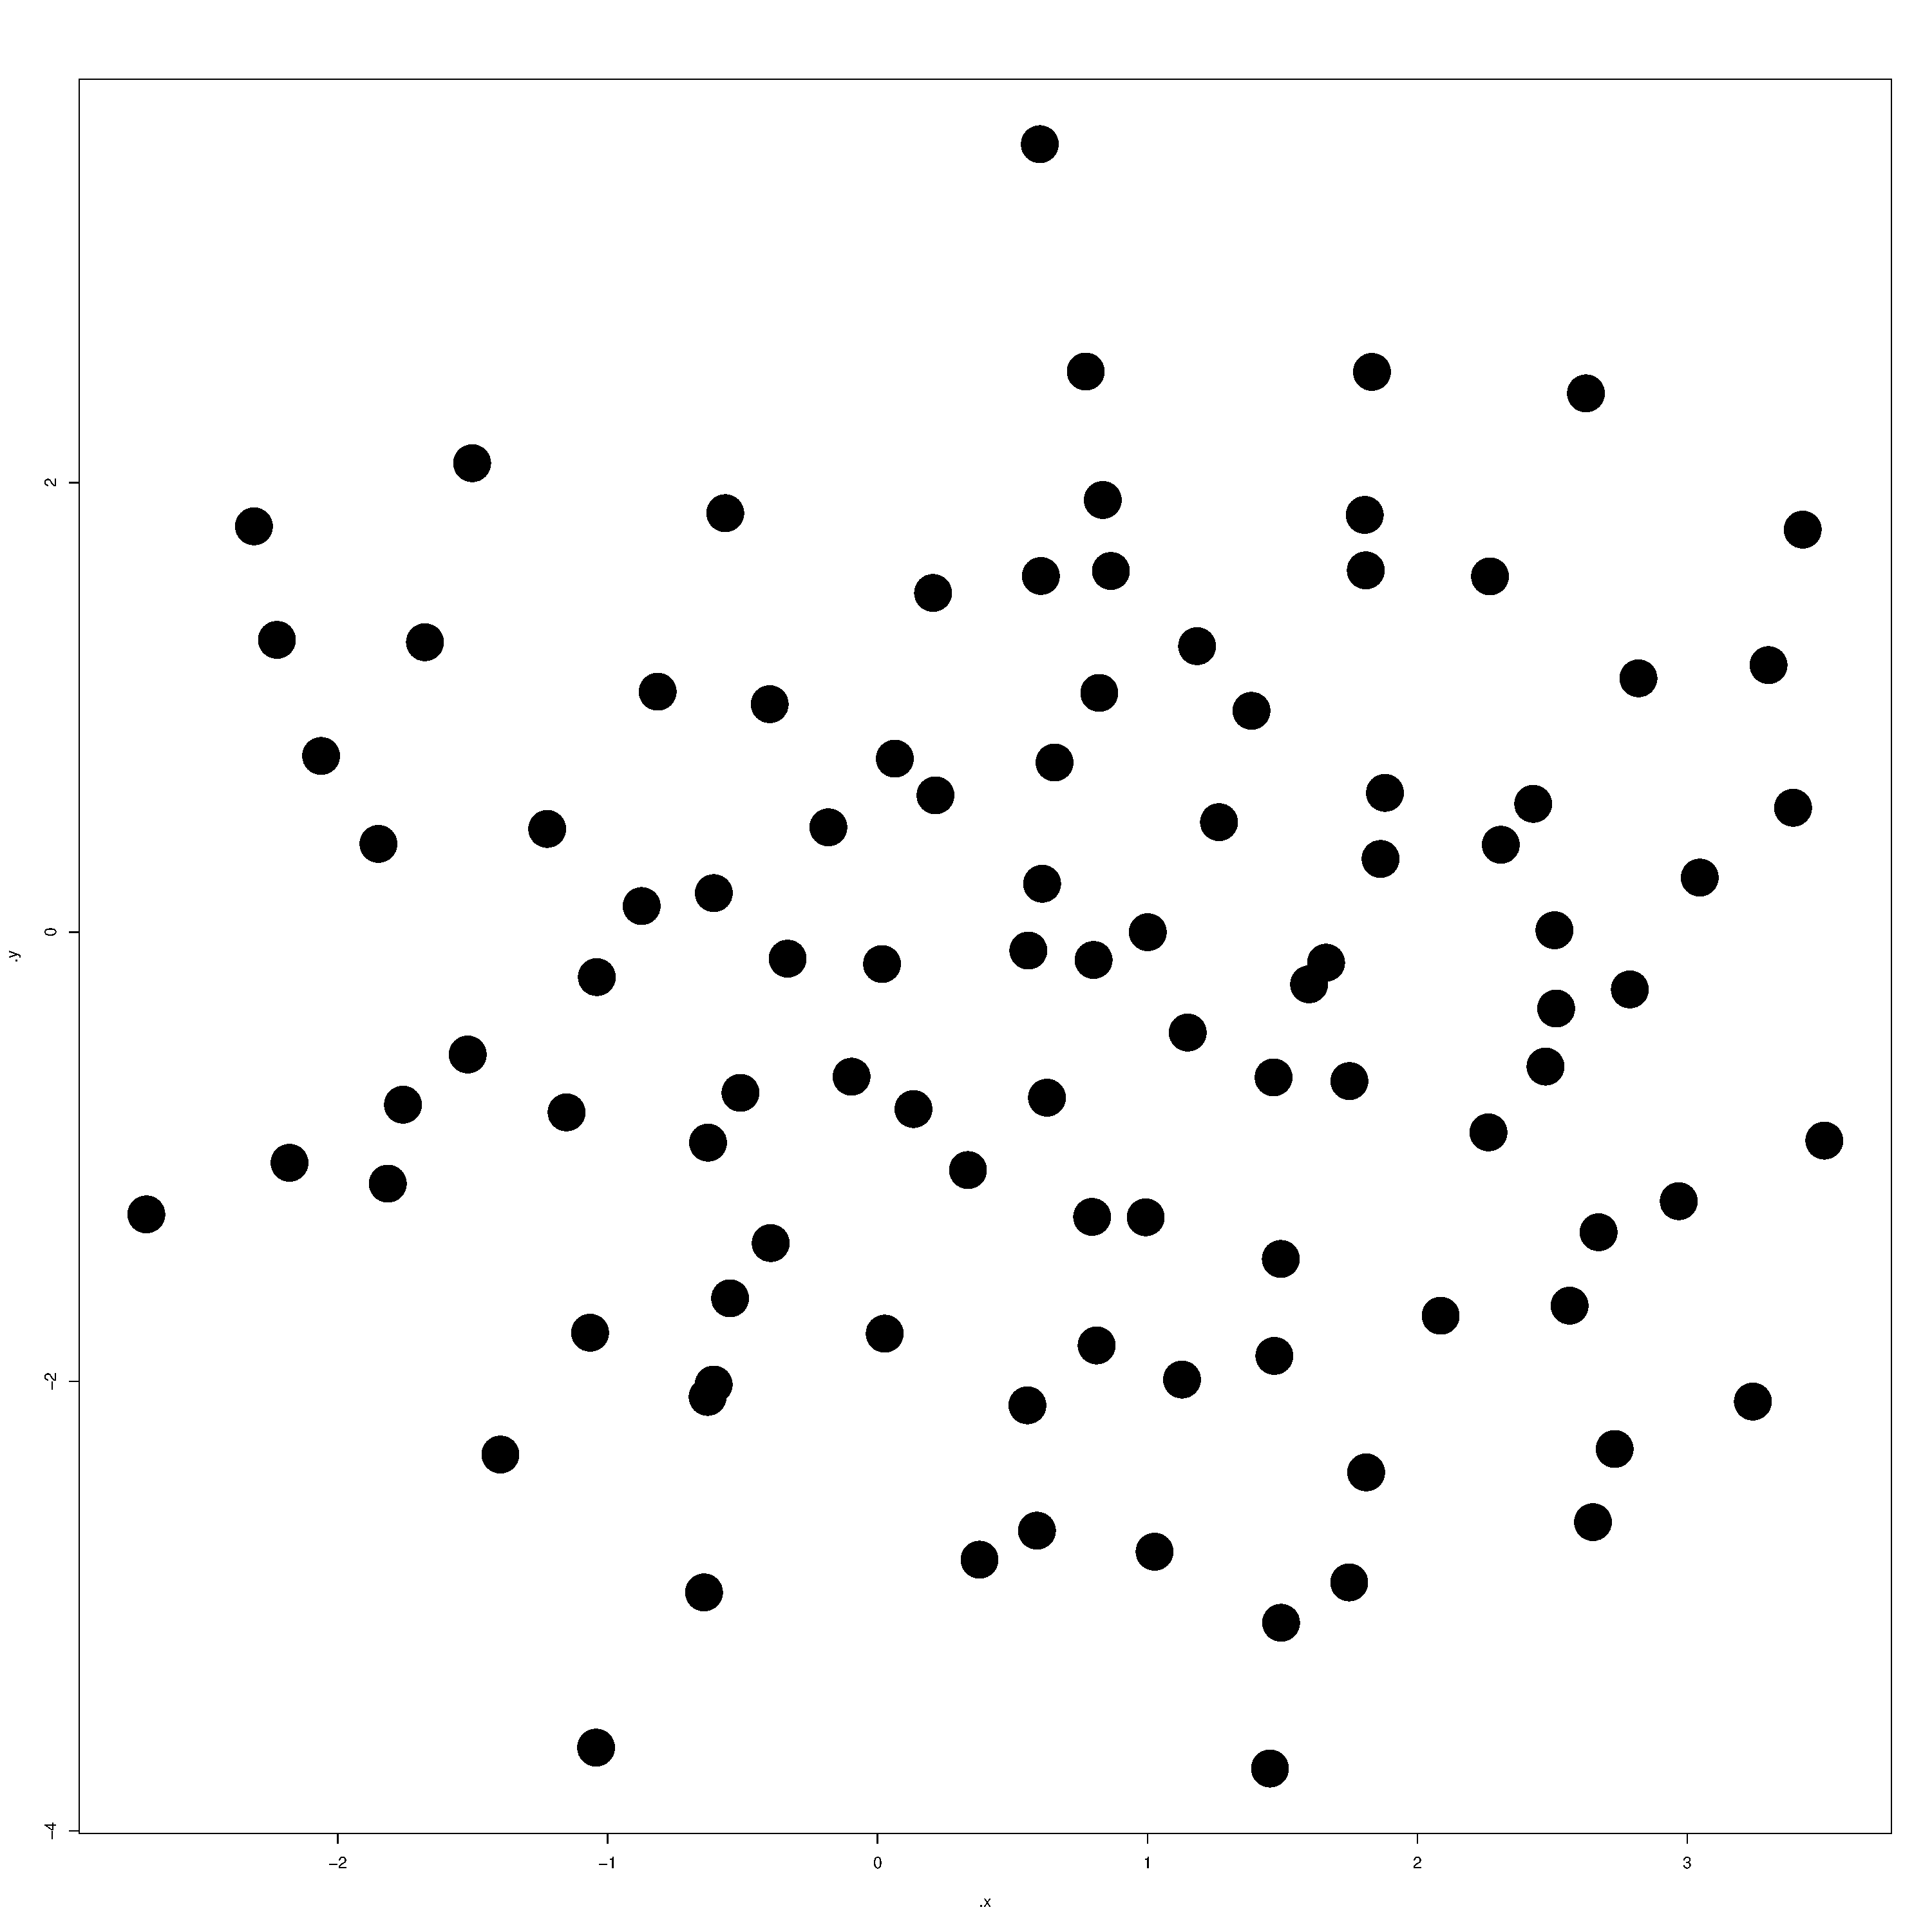
\includegraphics[height=2.5cm]{figures/blob_impl.pdf}
        \caption{No discernible clusters.}
    \end{subfigure}
    ~
    \begin{subfigure}[t]{0.45\textwidth}
	    \centering
        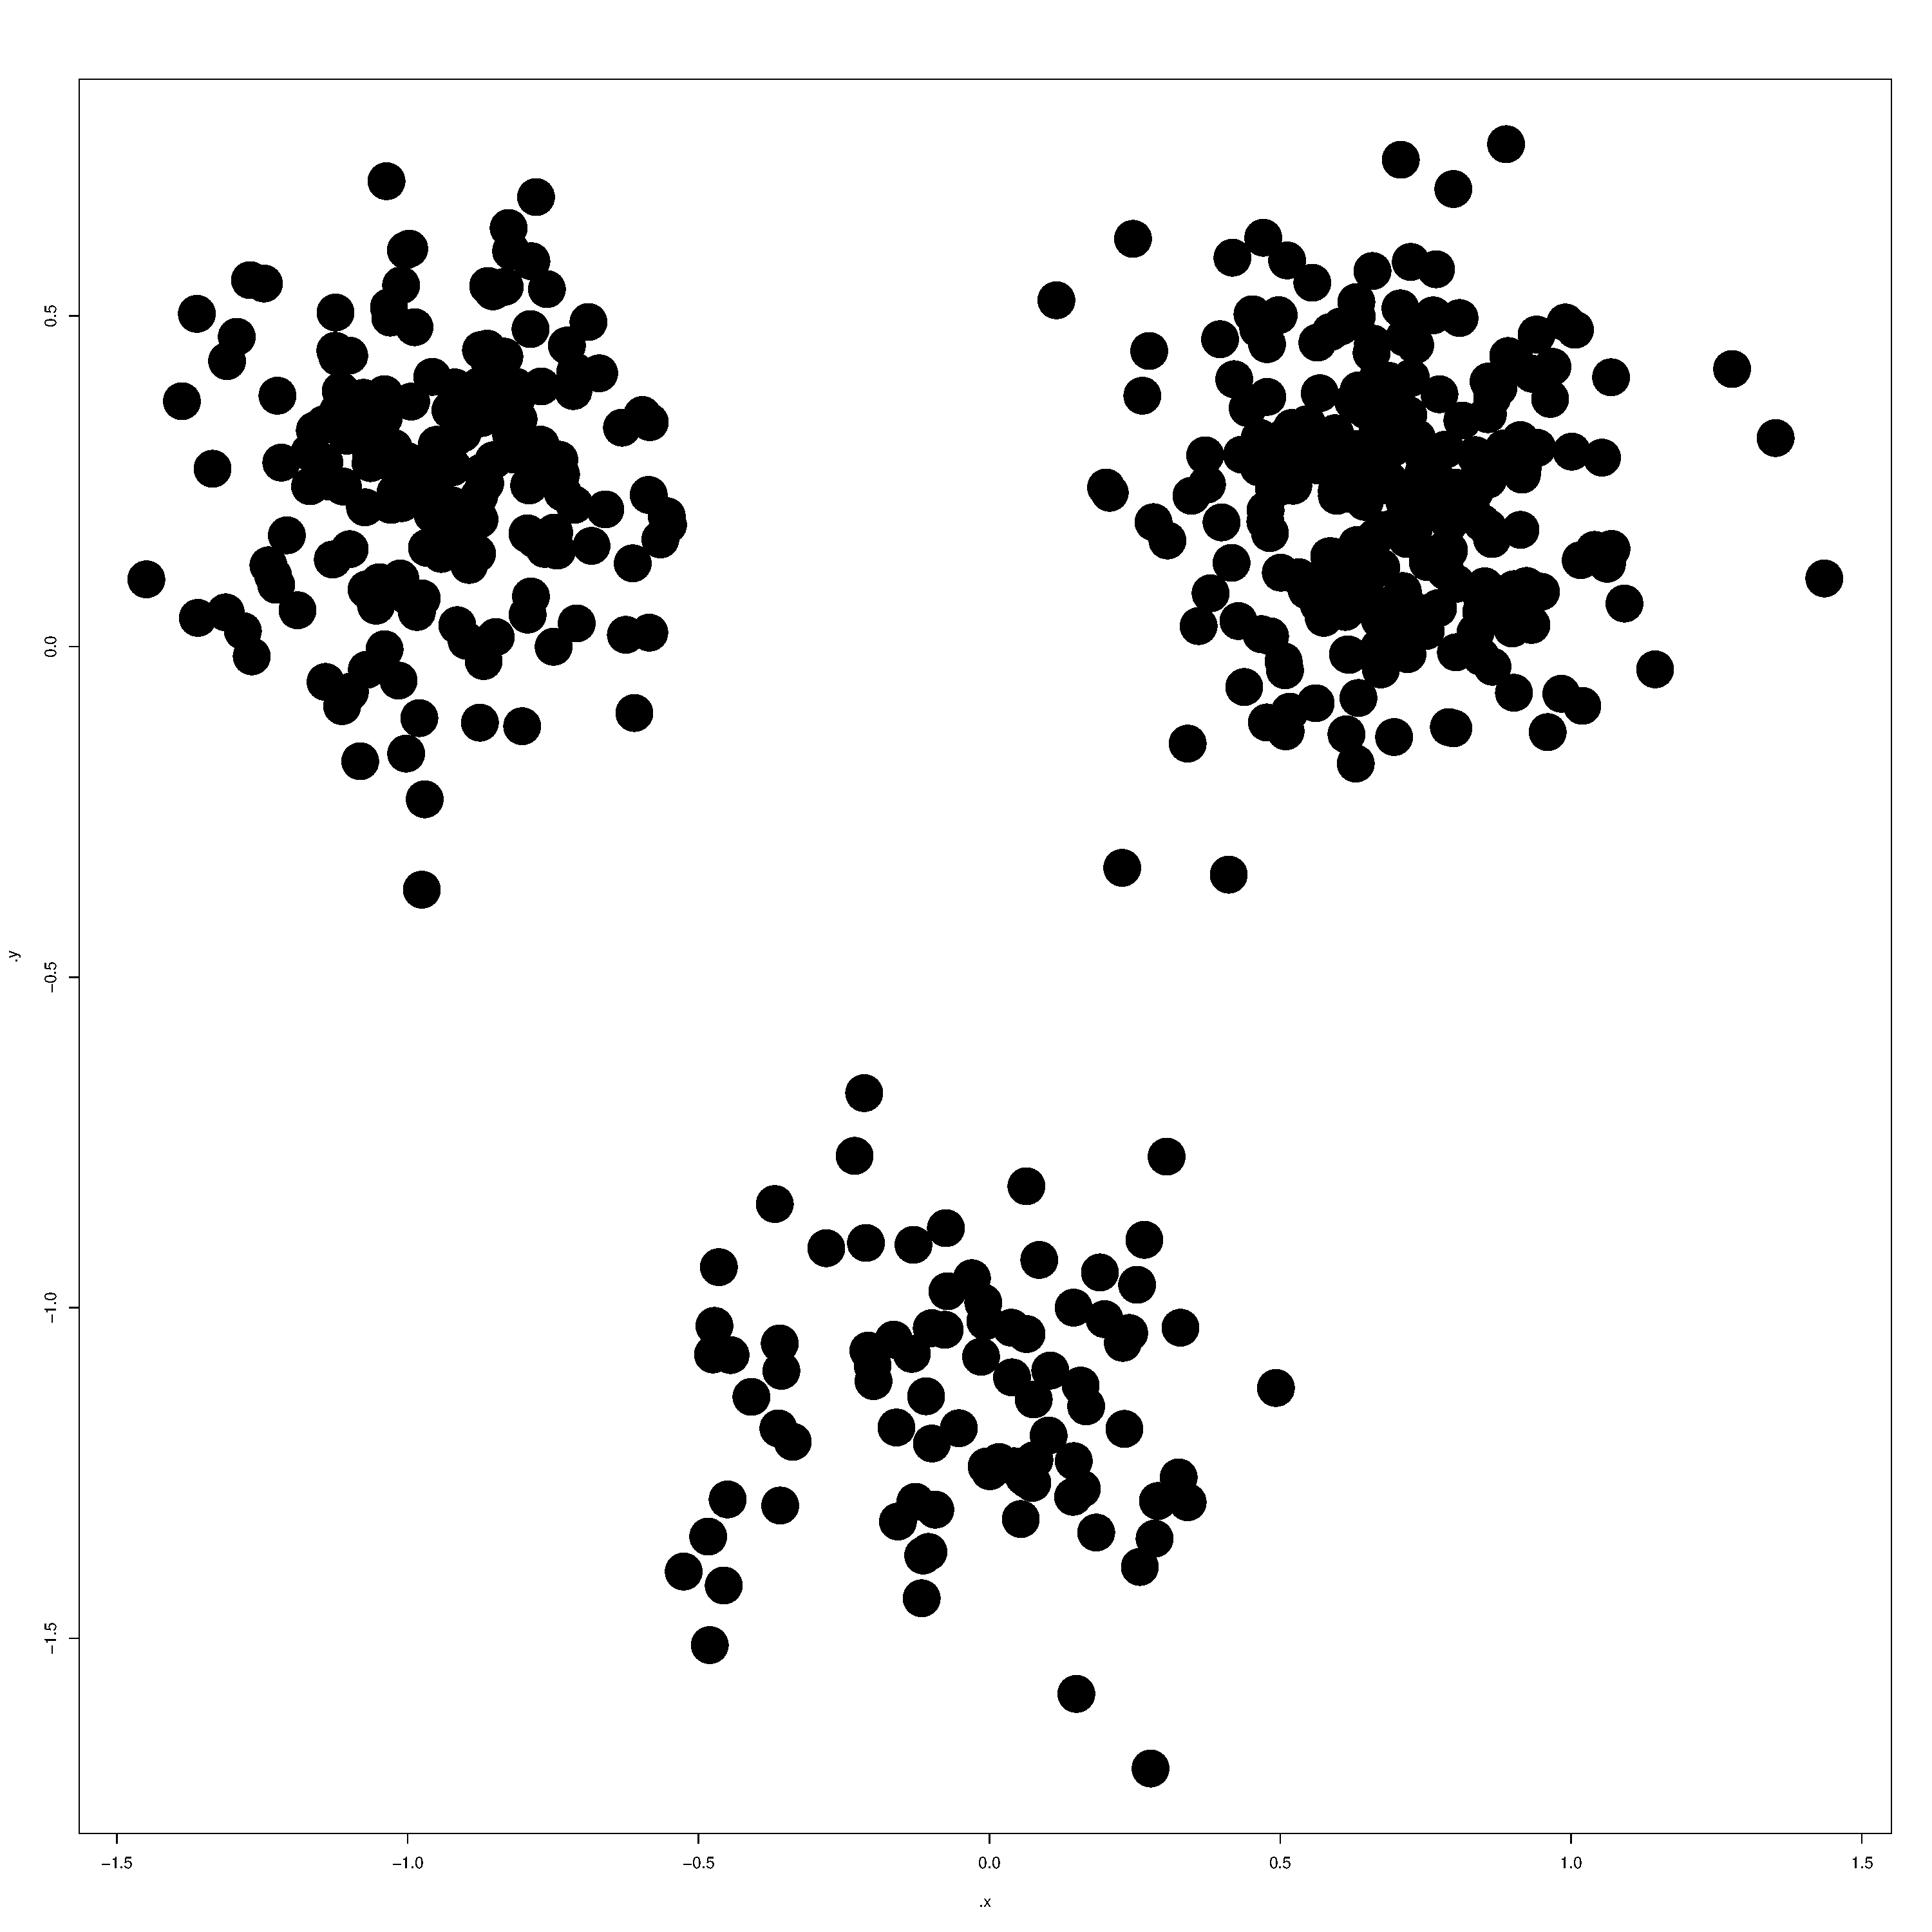
\includegraphics[height=2.5cm]{figures/clusters_impl.pdf}
        \caption{Three discernible clusters.}
    \end{subfigure}
    ~
    \begin{subfigure}[t]{0.45\textwidth}
	    \centering
        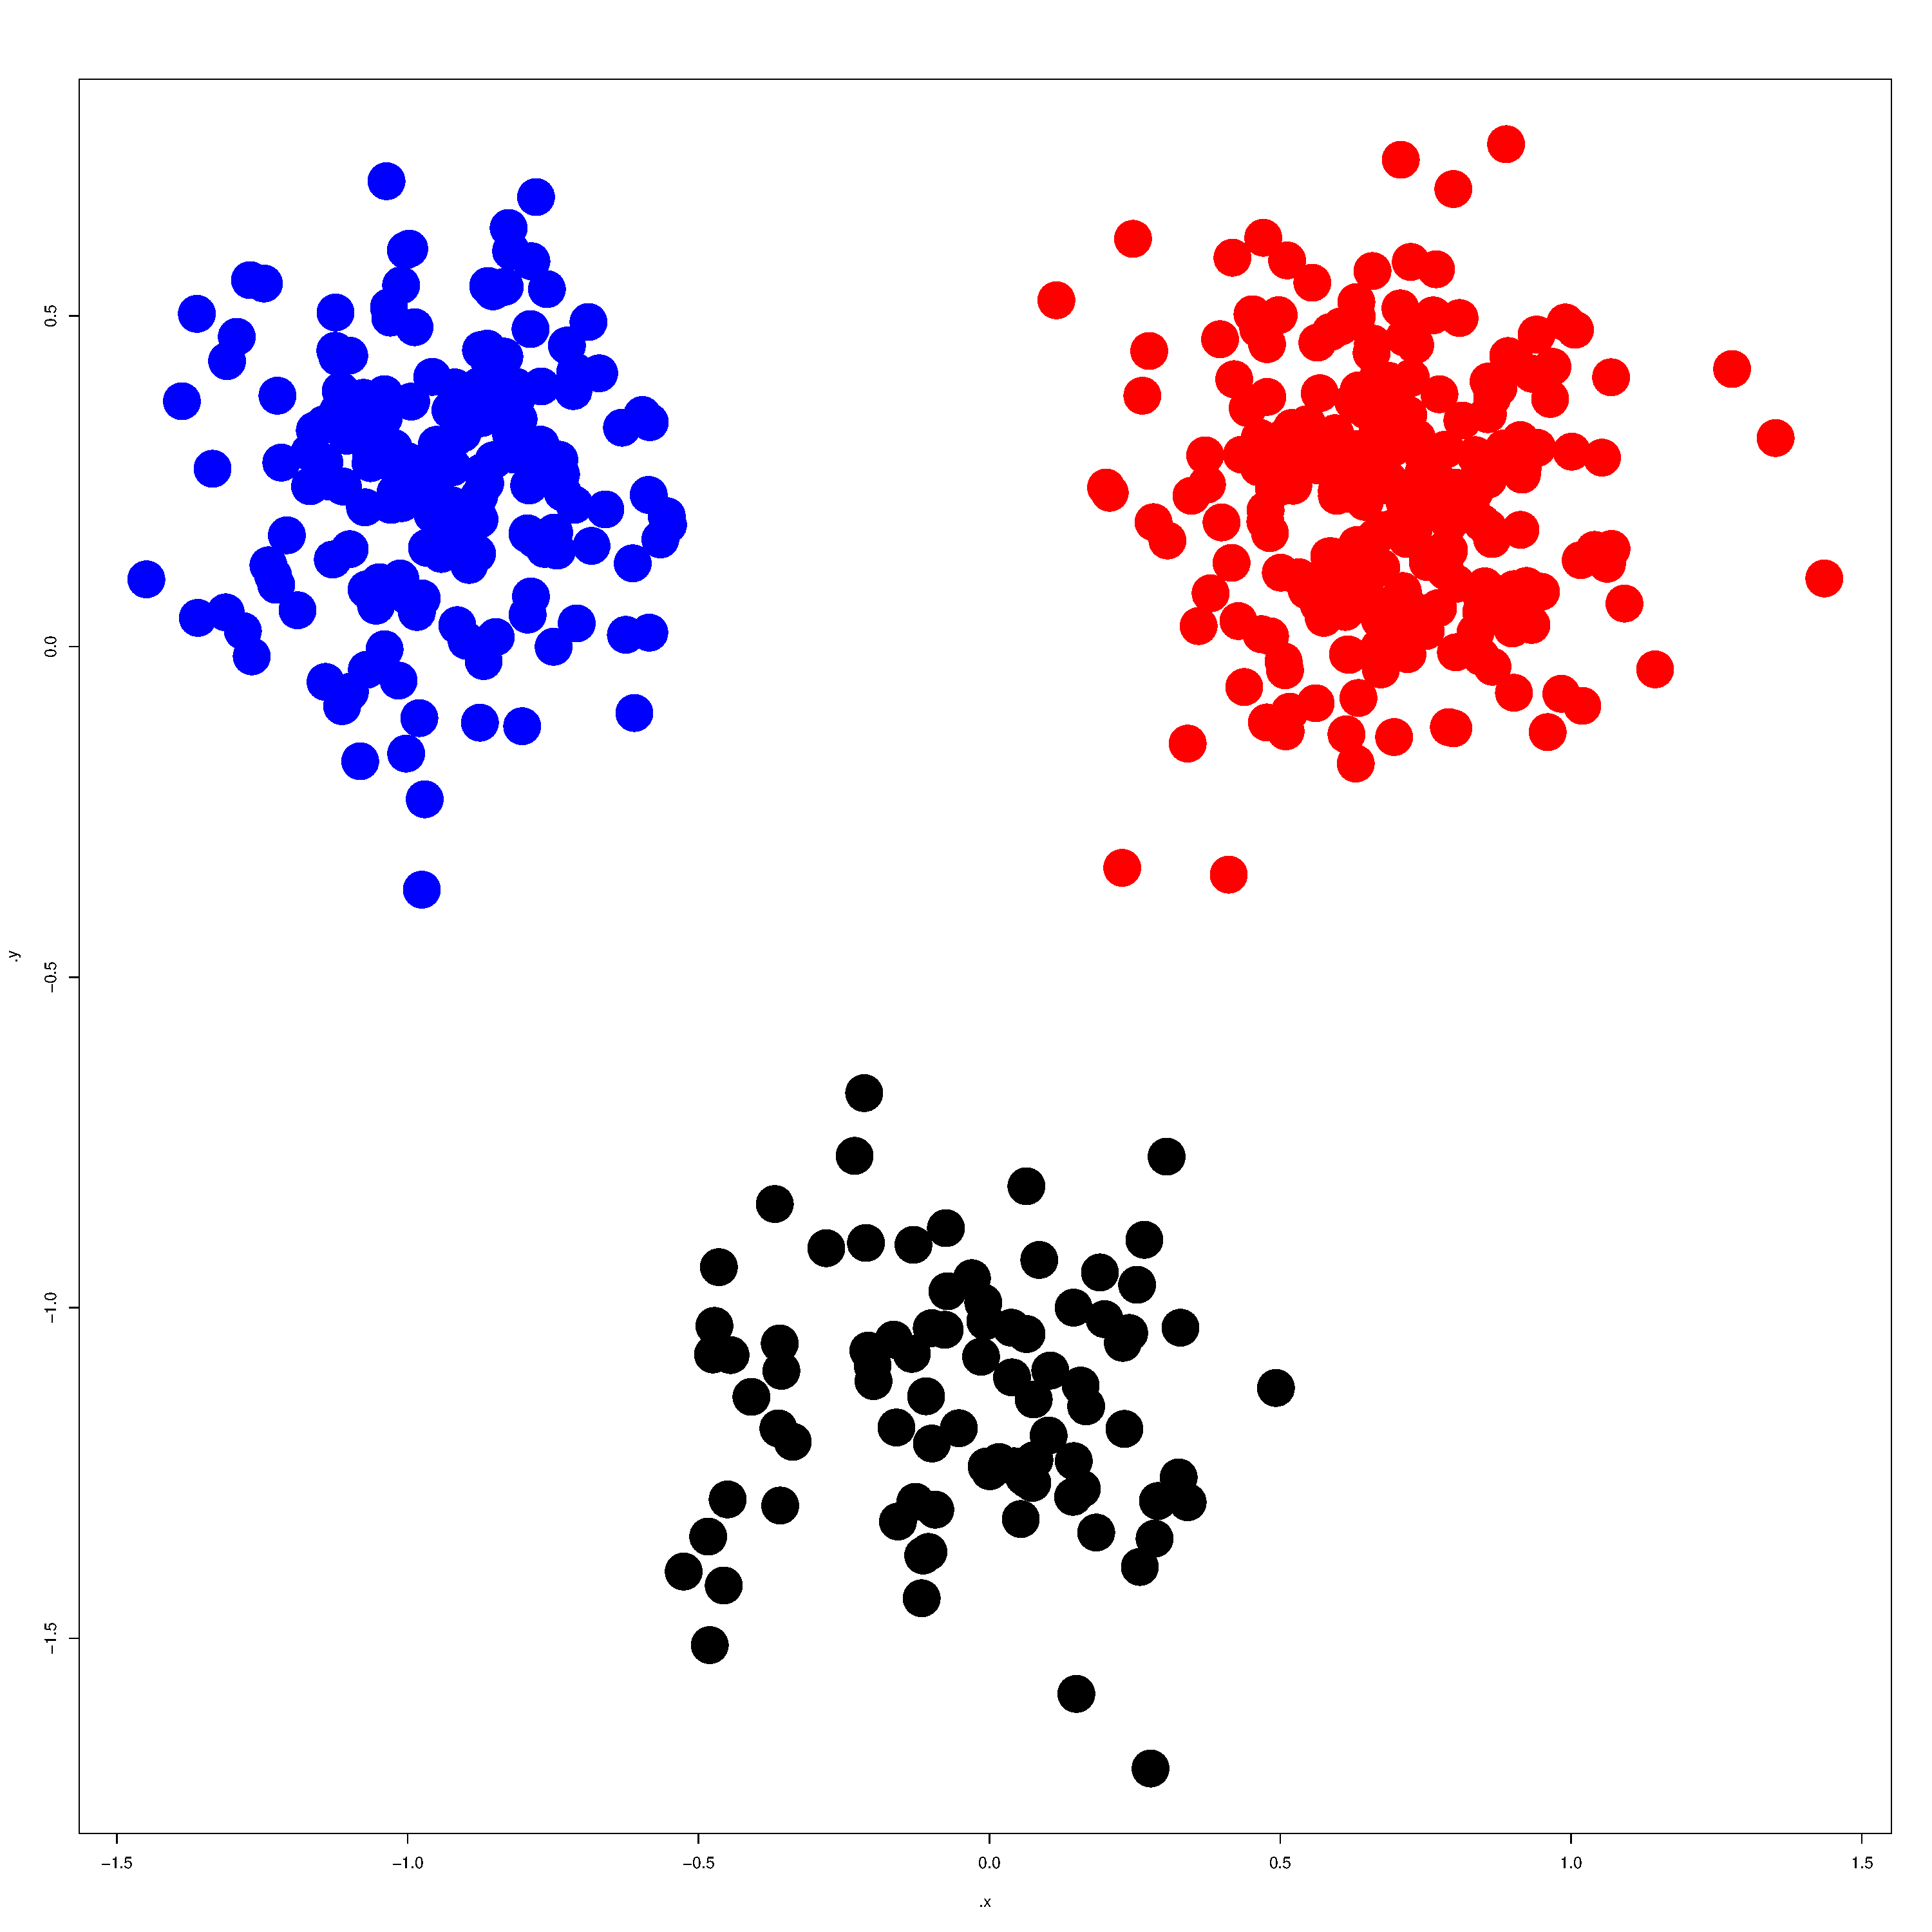
\includegraphics[height=2.5cm]{figures/clusters_expl.pdf}
        \caption{A match between clusters and class labels.}
    \end{subfigure}
    ~
    \begin{subfigure}[t]{0.45\textwidth}
	    \centering
        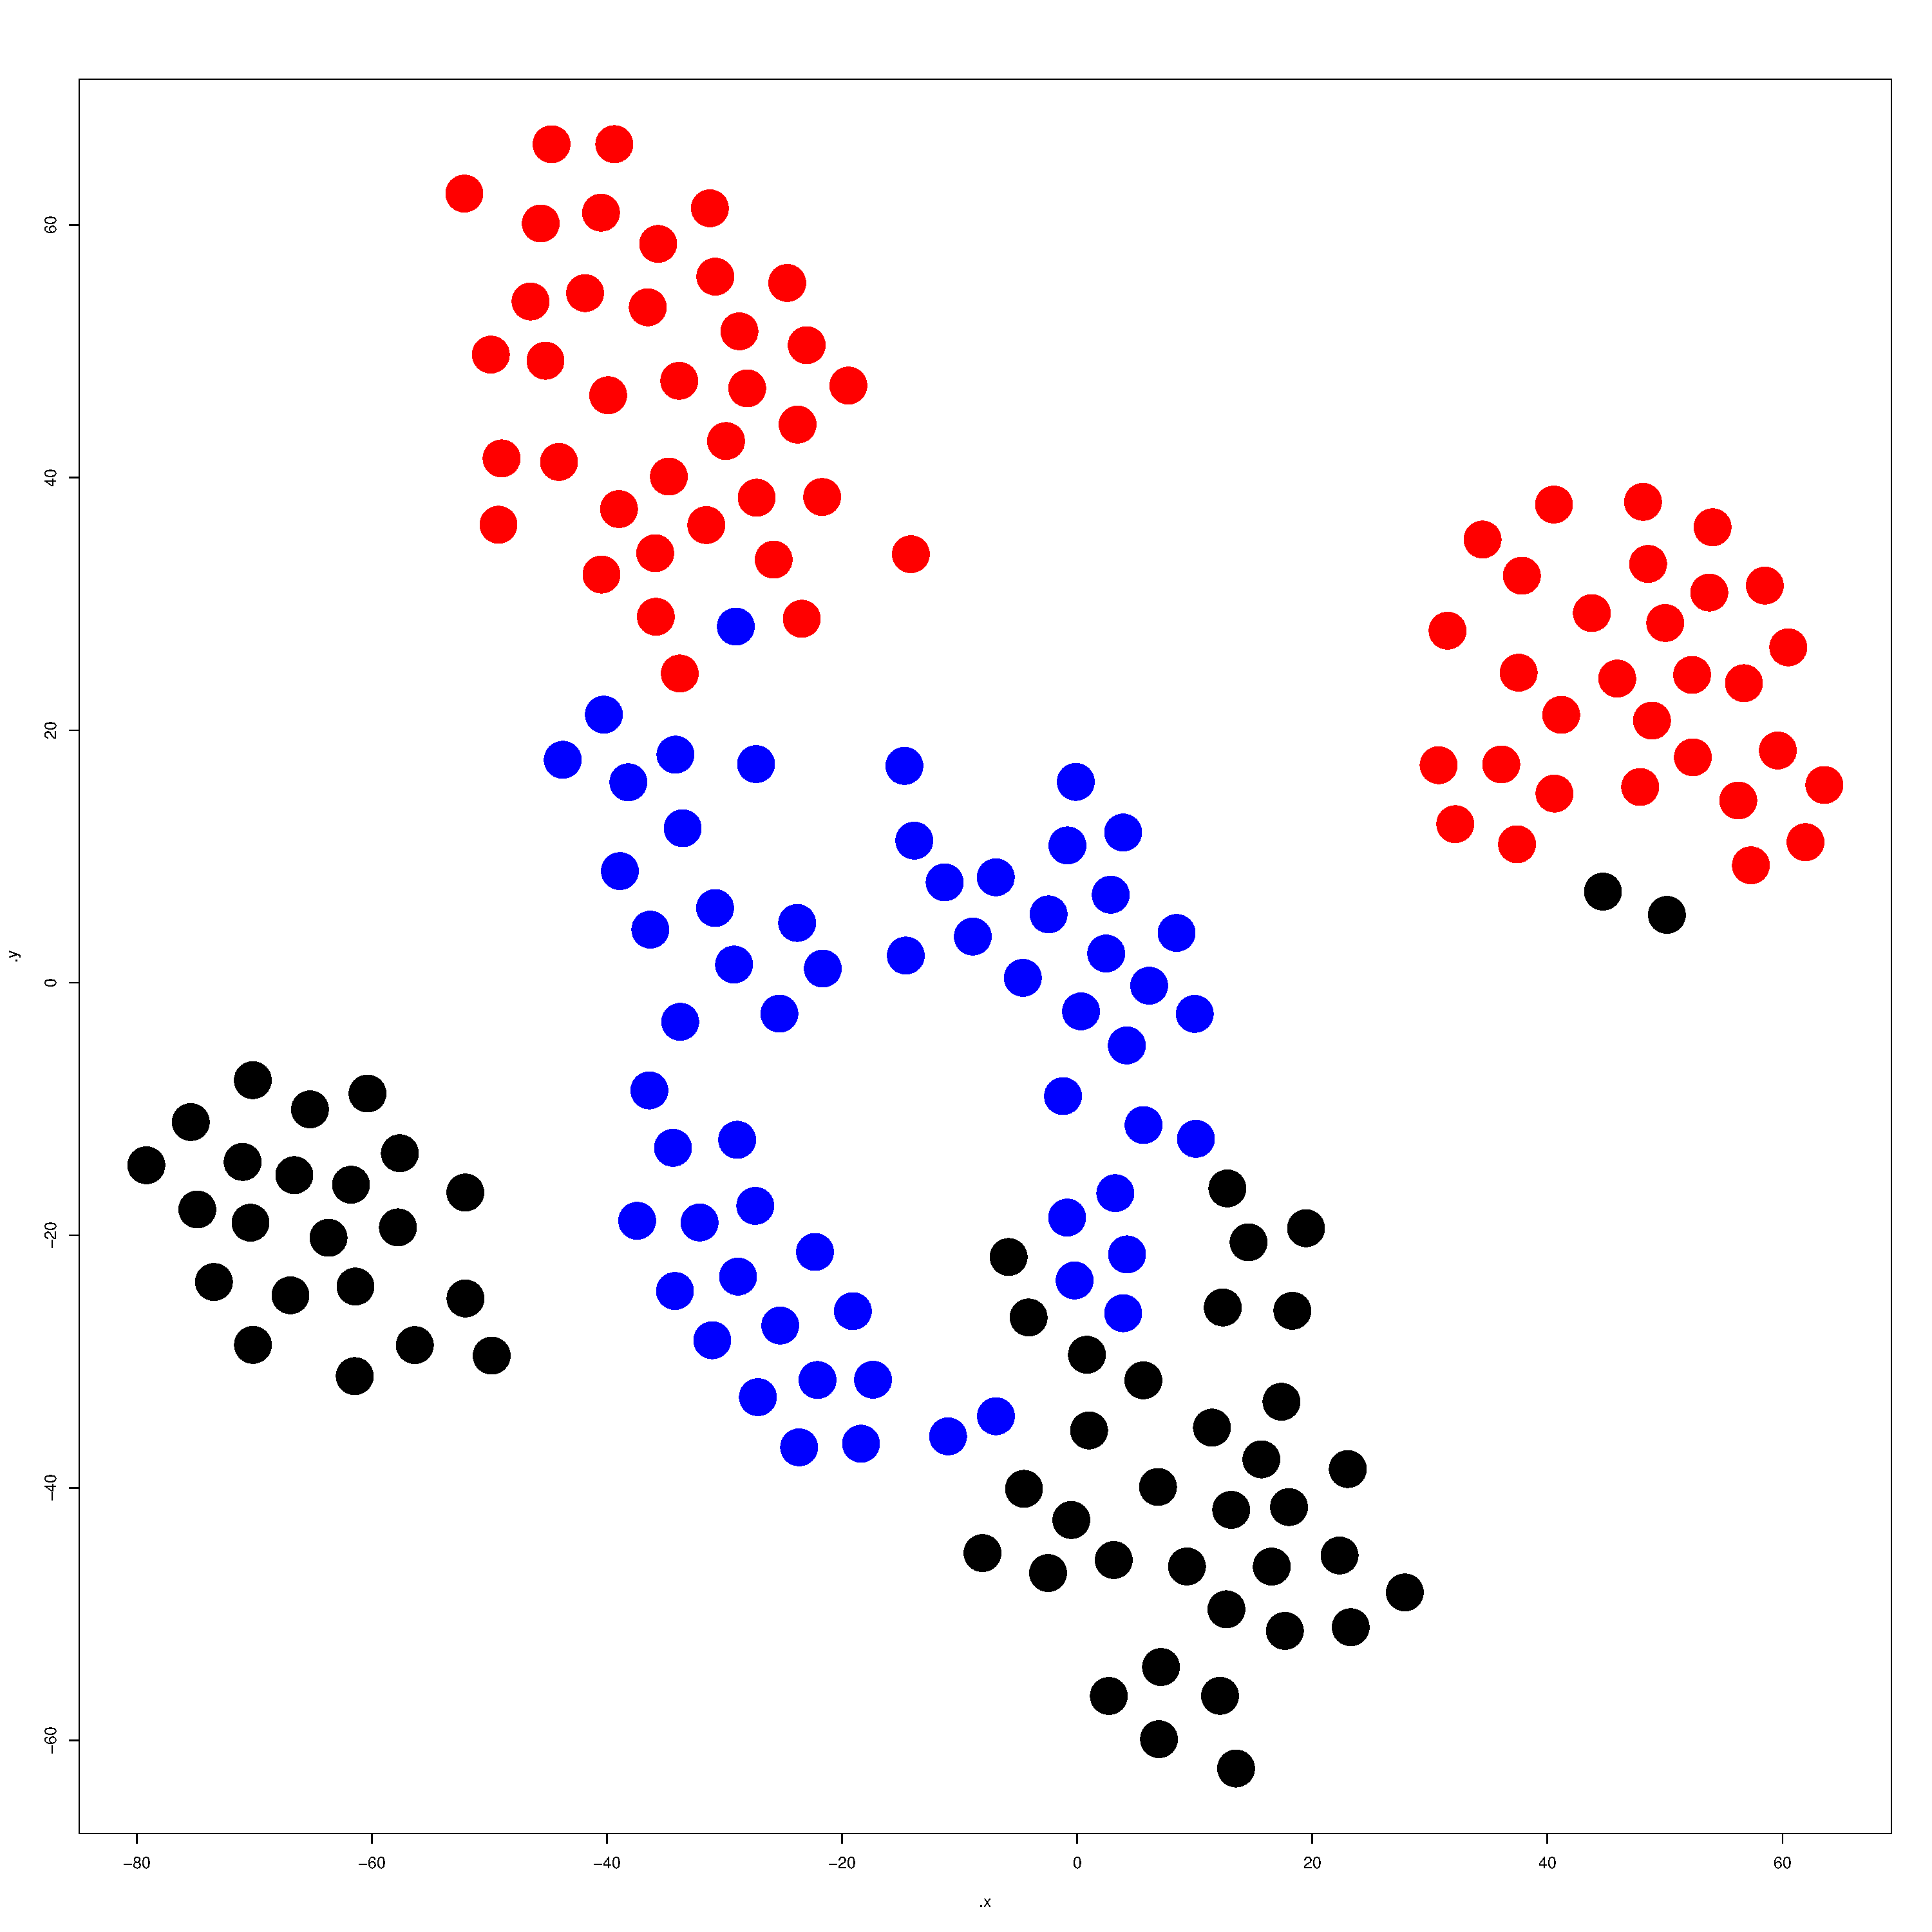
\includegraphics[height=2.5cm]{figures/clusters_expl_mismatch.pdf}
        \caption{A partial match between clusters and class labels.}
    \end{subfigure}
    ~
    \begin{subfigure}[t]{0.45\textwidth}
	    \centering
        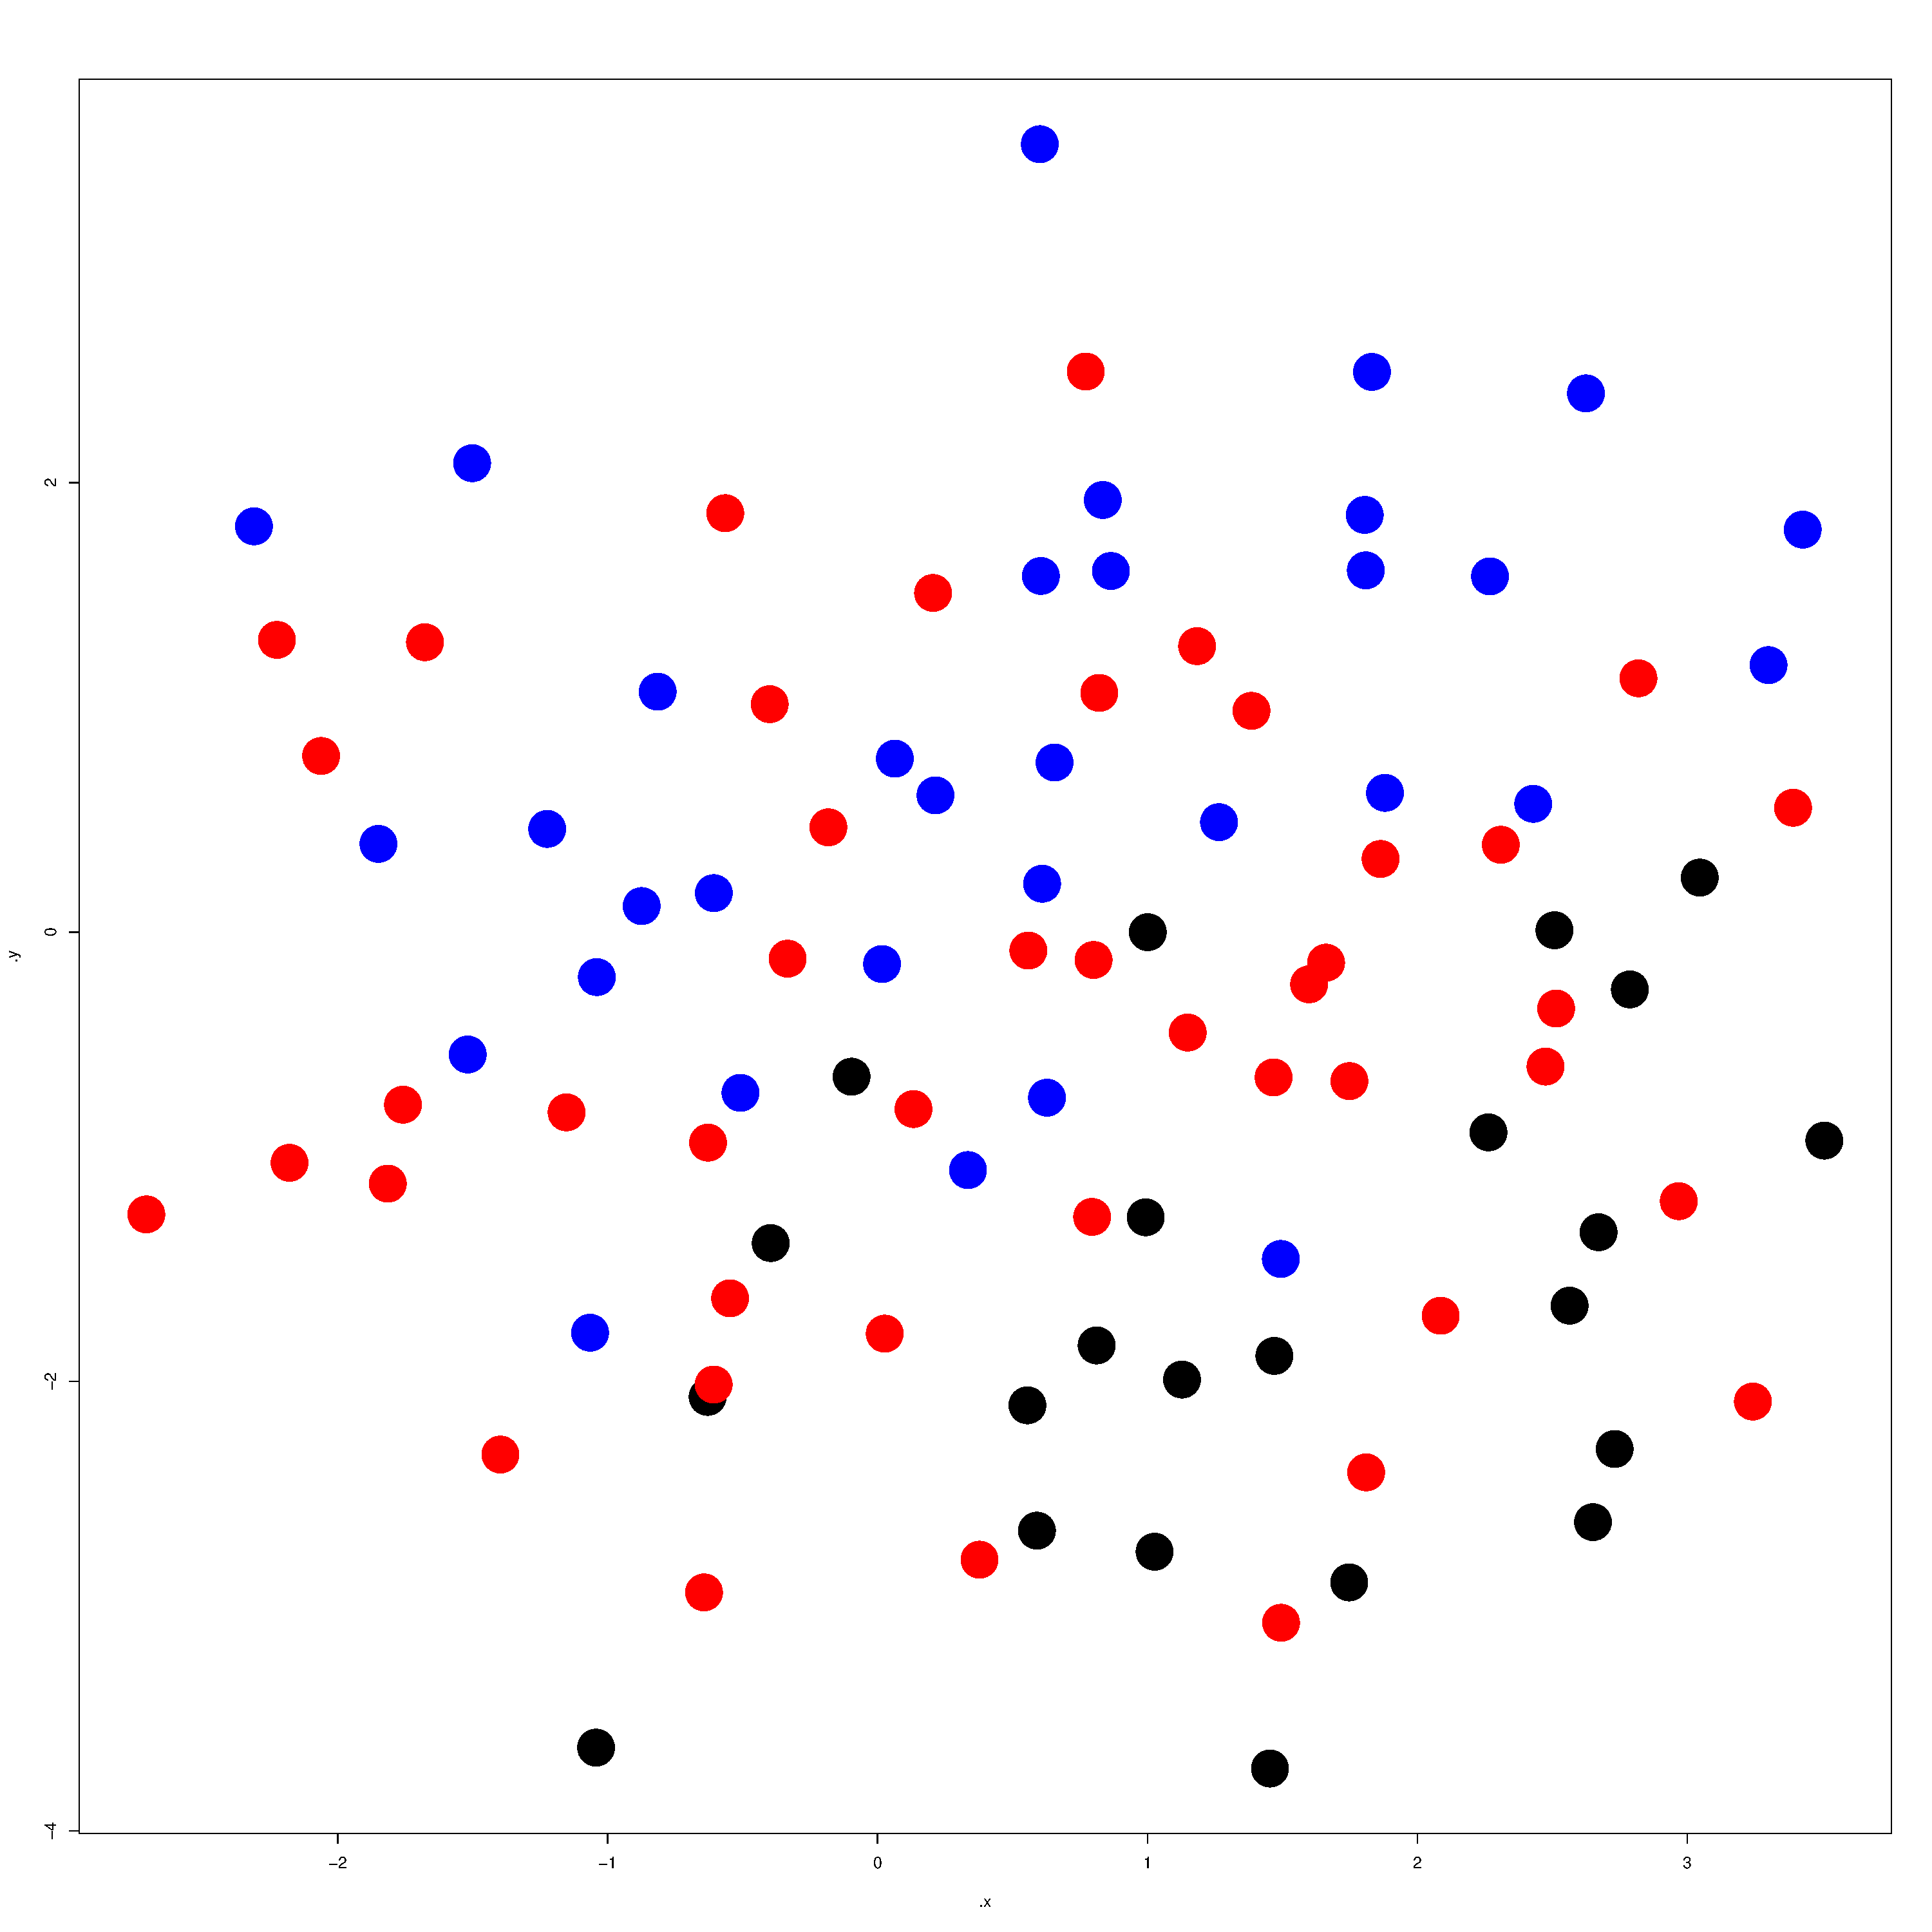
\includegraphics[height=2.5cm]{figures/blob_expl.pdf}
        \caption{No discernible class separation.}
    \end{subfigure}
	\caption
	[
	    Scatterplots of dimensionally reduced data illustrating tasks related to item clusters.
	]
	{
    	Example scatterplots of dimensionally reduced data illustrating tasks related to item clusters: Verifying the existence of clusters, naming clusters, and matching clusters and classes.
	}
	\centering
	\label{drvistasks:fig:clusters}
\end{figure}

%-|-|-|-|-|-|-|-|-|-|-|-|-|-|-|-|-|-|-|-|-|-|-|-|-|-|-|-|-|-|-|-|-|-|-|-|-

% %-------------------------------------------------------------------------

% \subsubsection{Verify Clusters}
% \label{drvistasks:tasks:verify-clusters}

%-------------------------------------------------------------------------

% \begin{figure}[!ht]
% 	\centering
% 	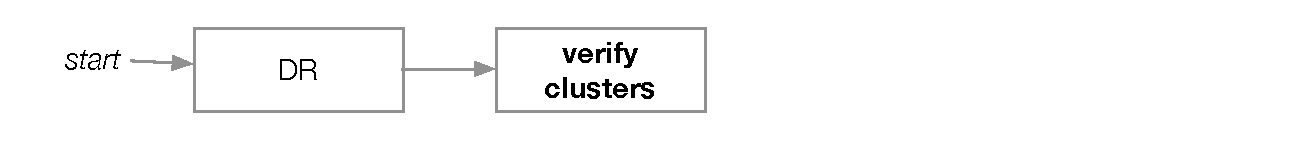
\includegraphics[width=\textwidth]{figures/drviztasks-identify-clusters.eps}
% 	\centering
% \end{figure}

\bstart{Verify clusters}
Analysts might seek to {\tt verify}\index{{\tt discover}} the hypothesis that clusters of items will be revealed in the dimensionally reduced\index{dimensionality reduction (DR)} data, or to {\tt verify}\index{{\tt discover}} hypotheses about specific conjectured clusters.
In order to {\tt discover}\index{{\tt discover}} clusters, analysts must {\tt locate}\index{{\tt locate}} and {\tt identify}\index{{\tt identify}} item clusters in the low-dimensional representation of the data; in the example of \autoref{drvistasks:fig:clusters}b, we can {\tt identify}\index{{\tt identify}} three clusters.

All ten of the analysts we spoke to were interested in verifying that clusters exist in their data. 
This task sequence\index{task!task sequence} is also captured by a discussion by \citet{Buja2002} about visualizing data following multidimensional scaling. 
The analysts we interviewed used a variety of visualization techniques when performing this task sequence\index{task!task sequence}, including two-dimensional monochrome scatterplots\index{visual encoding!scatterplot}, such as those depicted in \autoref{drvistasks:fig:clusters}a-b, as well as three-dimensional scatterplots\index{visual encoding!scatterplot!3D scatterplot}, \ac{SPLOM}s\index{visual encoding!scatterplot!scatterplot matrix (SPLOM)}, dendrograms\index{visual encoding!tree}, heat maps\index{visual encoding!heat map}, and density plots\index{visual encoding!density plot}. 

% %-------------------------------------------------------------------------

% \subsubsection{Name Clusters}
% \label{drvistasks:tasks:name-clusters}

% %-------------------------------------------------------------------------

% \begin{figure}[!ht]
% 	\centering
% 	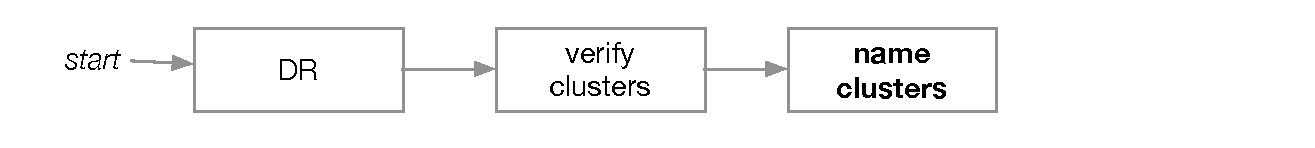
\includegraphics[width=\textwidth]{figures/drviztasks-name-clusters.eps}
% 	\centering
% \end{figure}

\bstart{Name clusters}
Once the existence of clusters has been verified, such as in the example of \autoref{drvistasks:fig:clusters}b, the next task\index{task} is often one of {\tt generating} hypotheses regarding the meaning of these clusters in the form of a name.
In this {\tt discover}\index{{\tt discover}} task\index{task}, an analyst will {\tt browse}\index{{\tt browse}} items within a cluster and attempt to {\tt summarize}\index{{\tt summarize}} the cluster with a meaningful name. 
In some cases, this name is made explicit, as the analyst will {\tt annotate}\index{{\tt annotate}} the cluster, thereby using the visual encoding\index{visual encoding} to {\tt produce}\index{{\tt produce}} new information about their data. 

Eight of the analysts who had previously {\it verified clusters} also attempted to {\it name clusters} in the course of their work, using the same visualization techniques. 
For instance,~\ref{drvistasks:analyst:HY} examined bibliometric data from a corpus of life sciences research literature, who attempted to {\tt identify}\index{{\tt identify}} and name clusters of related research concepts, such as {\it ``cancer''} or {\it ``RNA''}.

% %-------------------------------------------------------------------------

% \subsubsection{Match Clusters and Classes}
% \label{drvistasks:tasks:match-clusters}

% %-------------------------------------------------------------------------

% \begin{figure}[!ht]
% 	\centering
% 	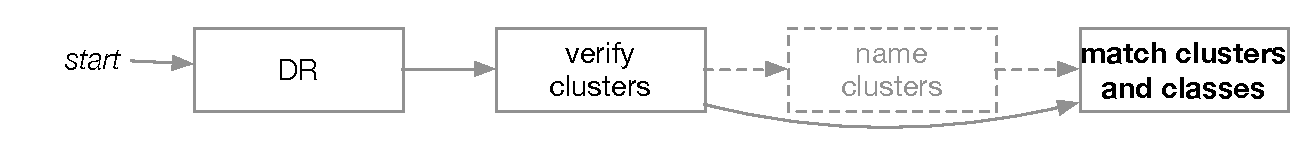
\includegraphics[width=\textwidth]{figures/drviztasks-match-clusters.eps}
% 	\centering
% \end{figure}

\bstart{Match clusters and classes}
The final task sequence\index{task!task sequence} we characterize is matching clusters with classes. 
The {\tt input}\index{{\tt input}} to this {\it match} task\index{task} is not only a set of item clusters, {\tt identified}\index{{\tt identify}} in the earlier {\it verify clusters} task\index{task}, but also a set of categorical class labels.
These classes might come directly with the data, be assigned using a clustering algorithm\index{algorithms!clustering} run by the analyst, or be the result of manual labeling. 
The analyst must {\tt verify}\index{{\tt discover}} a hypothesis that a cluster of items matches the class for those items. 
To {\tt discover}\index{{\tt discover}} a match, the analyst performs a {\tt lookup}\index{{\tt lookup}} for the class and cluster membership of an item in order to {\tt compare}\index{{\tt compare}} them, resulting in a match (as in \autoref{drvistasks:fig:clusters}c), otherwise referred to as a {\it true positive}, or a mismatch (as in \autoref{drvistasks:fig:clusters}d-e), which could either be a {\it true negative} or a {\it false negative}.
This task\index{task} was examined in our recent paper~\cite{Sedlmair2013}, a paper that offered guidance for choosing appropriate visualization techniques for dimensionally reduced\index{dimensionality reduction (DR)} data.

Naming the clusters is not a pre-requisite for this {\it match} task\index{task}, though we did encounter four analysts who reported performing both tasks\index{task} in succession (\ref{drvistasks:analyst:JB}, \ref{drvistasks:analyst:HL}, \ref{drvistasks:analyst:DH}, \ref{drvistasks:analyst:JS}); two other analysts performed this task\index{task} without previously naming the clusters they identified\index{{\tt identify}} (\ref{drvistasks:analyst:KA}, \ref{drvistasks:analyst:AC}).
Typically, this task\index{task} was performed using two-dimensional scatterplots\index{visual encoding!scatterplot}, wherein the points were coloured using the class labels; \ac{SPLOM}s\index{visual encoding!scatterplot!scatterplot matrix (SPLOM)}, interactive and non-interactive three-dimensional scatterplots\index{visual encoding!scatterplot}, and node-link graphs were also used.
Note that the visual separability of colour-coded clusters differs perceptually from the separability of monochrome clusters, as described in our recent taxonomy of cluster separation factors~\cite{Sedlmair2012a}. 
These perceptual differences should be taken into account particularly when determining which experimental stimuli for use in controlled experiments.

A possible outcome of this task sequence\index{task!task sequence} is a partial match between classes and clusters: there may be more clusters than classes, or vice versa.
In cases where there are more clusters than class labels, illustrated in \autoref{drvistasks:fig:clusters}d, this outcome suggests that the class labels may not capture a finer-grained cluster structure in the data, as was the case for the investigative journalist\index{journalism} that we interviewed (\ref{drvistasks:analyst:JS}). 
In cases where there are more classes than clusters, illustrated in \autoref{drvistasks:fig:clusters}e, this result may either be a {\it true negative}, in which perfect class separation is not possible, or a {\it false positive}~\cite{Sedlmair2013}.
If this mismatch is suspected to be a {\it false negative}, Sedlmair~\etal~recommend {\tt selecting}\index{{\tt select}} other dimensions to visualize, using other design choices such as a \ac{SPLOM}\index{visual encoding!scatterplot!scatterplot matrix (SPLOM)}, or revisiting the choice of \ac{DR}\index{dimensionality reduction (DR)} technique. 

%-------------------------------------------------------------------------
%-------------------------------------------------------------------------

\section{A Task Typology Revisited}
\label{drvistasks:typology}

%-------------------------------------------------------------------------
%-------------------------------------------------------------------------

The analysts that we interviewed hailed from very different domains, each using a different terminology to describe their work processes\index{work domain analysis}.
For instance, we needed a way to compare how {\it diagnosing cancer patients based on their genomic data} (\ref{drvistasks:analyst:AC}) was like {\it classifying types of human motion through the use of sensors attached to the body} (\ref{drvistasks:analyst:KA}).
We required an abstract vocabulary\index{task!task abstraction} for describing and comparing the work processes of these analysts.

For this reason, we used our typology\index{task!task typology} of abstract visualization tasks\index{task!task abstraction}, introduced in \autoref{ch:typology}, which provided a domain-agnostic vocabulary and framework for describing visualization tasks\index{task} in terms of {\it why}\index{{\tt why}}, {\it what}\index{{\tt what}}, and {\it how}\index{{\tt how}}.
By describing a task\index{task} in this manner, we can link {\tt outputs}\index{{\tt output}} and {\tt inputs}\index{{\tt input}} to describe sequences\index{task!task sequence} of interdependent tasks\index{task}, which Norman would refer to as {\it activities}~\cite{Norman2005}. 
% This typology has already been used to characterize the tasks of journalists~\cite{Brehmer2014}\footnote{This classification of journalists' tasks is documented in \autoref{ch:overview}.} and bioinformaticians~\cite{Mirel2014}. 
We use it here to describe task sequences\index{task!task sequence} relating to visualizing dimensionally reduced\index{dimensionality reduction (DR)} data across multiple domains.

Our analysis concentrated on the {\it why}\index{{\tt why}} and {\it what}\index{{\tt what}} aspects of the tasks\index{task} pertaining to dimensionally reduced\index{dimensionality reduction (DR)} data, as summarized in \autoref{drvistasks:fig:drviztasks}.
We chose not to be prescriptive about {\it how}\index{{\tt how}} these task sequences\index{task!task sequence} should best be supported by visualization techniques; instead, we described the variety of techniques used by the analysts that we interviewed for each task sequence\index{task!task sequence}, as summarized in \autoref{drvistasks:tab:summary}.

%-|-|-|-|-|-|-|-|-|-|-|-|-|-|-|-|-|-|-|-|-|-|-|-|-|-|-|-|-|-|-|-|-|-|-|-|-

\begin{figure}
	\centering
	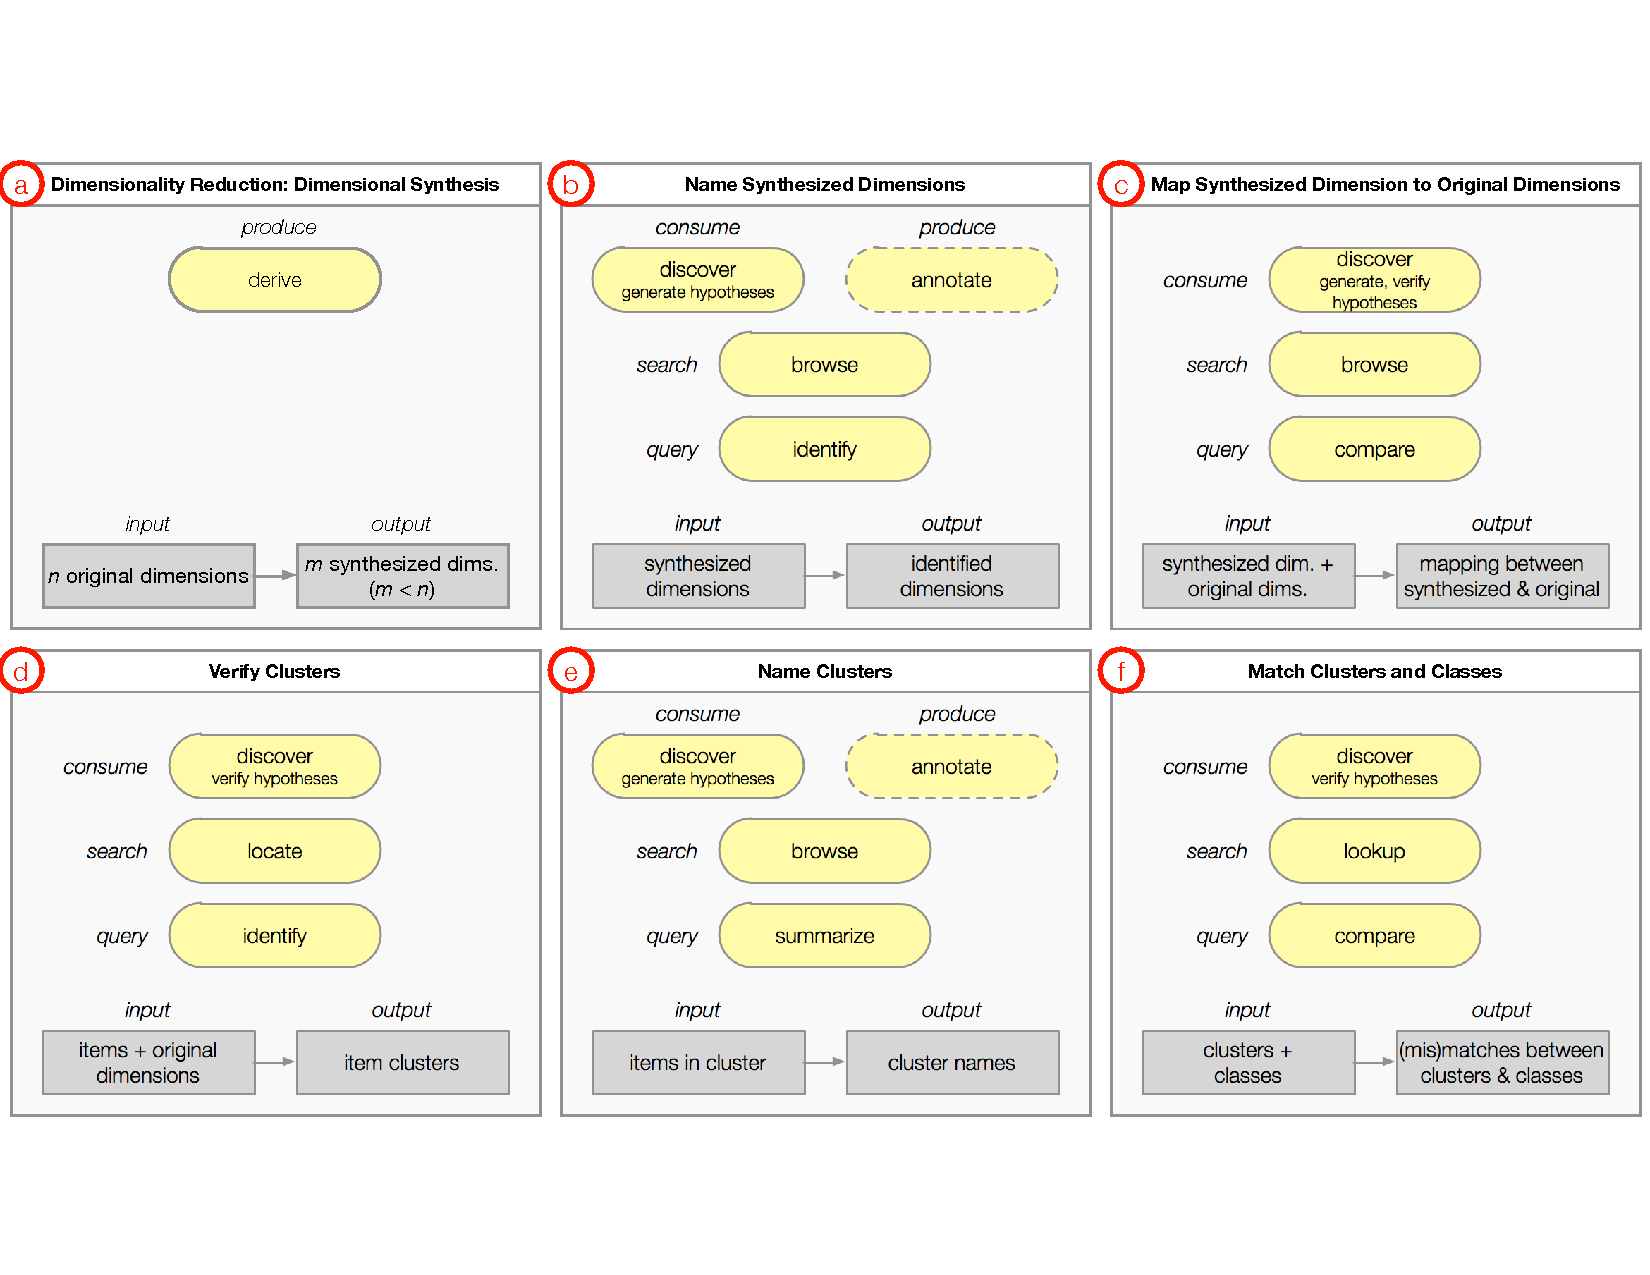
\includegraphics[width=\textwidth]{figures/drviztasks.pdf}
	\caption
	[
	    Six tasks related to dimensionally reduced data, characterized using our abstract task typology.
	]
	{
	    Six tasks related to dimensionally reduced data, characterized using our abstract task typology introduced in \autoref{ch:typology}, which describes \textsl{why} the data is being visualized at multiple levels of abstraction (yellow) and \textsl{what} {\tt inputs} and {\tt outputs} a task has (grey). These tasks are combined to form the task sequences described in \autoref{drvistasks:tasks}.
	}
	\centering
	\label{drvistasks:fig:drviztasks}
\end{figure}

%-|-|-|-|-|-|-|-|-|-|-|-|-|-|-|-|-|-|-|-|-|-|-|-|-|-|-|-|-|-|-|-|-|-|-|-|-

The analysts we interviewed were all interested in {\tt discovery}, which involves the {\tt generation} and {\tt verification} of hypotheses. 
\autoref{drvistasks:fig:drviztasks}b-f show which tasks\index{task} relate to {\tt hypothesis generation}\index{{\tt discover}} and which relate to {\tt hypothesis verification}\index{{\tt discover}}. 
The graphical depiction also shows which task\index{task} can be associated with pure {\tt consumption} of information and which task\index{task} can additionally lead to the {\tt production} of new information.
When consuming information, an analyst will {\tt search}\index{{\tt search}} for targets within a visual encoding\index{visual encoding}.
Whether the location and identity of these targets is known a priori will determine the type of {\tt search}\index{{\tt search}}. 
In tasks\index{task} related to visualizing dimensionally reduced\index{dimensionality reduction (DR)} data, we found that {\tt search}\index{{\tt search}} strategies used by analysts were either {\tt browse}\index{{\tt browse}}, {\tt locate}\index{{\tt locate}}, or {\tt lookup}\index{{\tt lookup}}, as indicated in \autoref{drvistasks:fig:drviztasks}b-f. 
Once targets are found, an analyst will execute some form of {\tt query}\index{{\tt query}}: they might {\tt identify}\index{{\tt identify}} a single target, such as an item cluster, {\tt compare}\index{{\tt compare}} multiple targets, such as values along a synthesized dimension to values along an original dimension, or {\tt summarize}\index{{\tt summarize}} all the targets, such as when {\it naming a cluster}. 

\bstart{Dependencies} 
The task sequences\index{task!task sequence} described in \autoref{drvistasks:tasks} contain dependencies. 
For example, in order to {\it match clusters and classes}, an analyst must first {\it verify}\index{{\tt discover}} that clusters exist. 
Each of the sequences\index{task!task sequence} also depend on the {\tt output}\index{{\tt output}} of \ac{DR}\index{dimensionality reduction (DR)} techniques, the {\tt derived}\index{{\tt derive}} synthetic dimensions.  
The application of \ac{DR}\index{dimensionality reduction (DR)} to a set of original dimensions is itself a task\index{task}, as shown in \autoref{drvistasks:fig:drviztasks}a. 
However, unlike the other tasks\index{task} described in this chapter, it is about neither hypothesis generation nor verification, but rather about {\tt producing}\index{{\tt produce}} new information intended to support subsequent tasks\index{task}.

While the distinctions between these tasks\index{task} and task sequences\index{task!task sequence} may seem obvious in hindsight, we initially struggled to find a vocabulary and framework that would allow us to distinguish between these task sequences\index{task!task sequence} and their interdependencies.
Our task typology\index{task!task typology}, introduced in \autoref{ch:typology}, allows us to describe these task sequences\index{task!task sequence} explicitly, whereas they were implicit in previous work combining \ac{DR}\index{dimensionality reduction (DR)} and visualization.

\bstart{Extended typology}
\autoref{drvistasks:fig:typology} reproduces the {\it why}\index{{\tt why}} part of an extended task typology~\cite{Munzner2014}\footnote{We comment further on the the extensions to our typology in \autoref{conclusions:typology:extension}.}.

%-|-|-|-|-|-|-|-|-|-|-|-|-|-|-|-|-|-|-|-|-|-|-|-|-|-|-|-|-|-|-|-|-|-|-|-|-

\begin{figure}
	\centering
	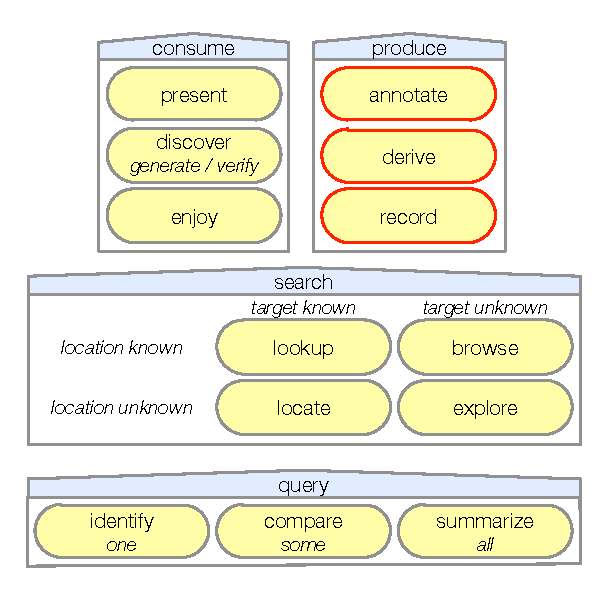
\includegraphics[width=0.7\textwidth]{figures/typology-why.eps}
	\caption
	[
	    A refinement to the \textsl{why} part of our abstract task typology.
	]
	{
    	The \textsl{why} part of our abstract task typology from \autoref{ch:typology}, with the refinement (emphasized in red) that the actions of {\tt annotate}, {\tt record}, and {\tt derive} are forms of {\tt produce}~\cite{Munzner2014}.
    }
    \centering
	\label{drvistasks:fig:typology}
\end{figure} 

%-|-|-|-|-|-|-|-|-|-|-|-|-|-|-|-|-|-|-|-|-|-|-|-|-|-|-|-|-|-|-|-|-|-|-|-|-

The changes relevant to our analysis in this chapter pertain to three actions: an analyst may {\tt annotate}\index{{\tt annotate}} information, {\tt derive}\index{{\tt derive}} new information from existing, or {\tt record}\index{{\tt record}} their use of a visualization tool so as to provide analytical provenance or to facilitate subsequent presentations of the visualized data. 
The terms {\tt annotate}\index{{\tt annotate}}, {\tt derive}\index{{\tt derive}}, and {\tt record}\index{{\tt record}} were previously attributed to families of interaction\index{interaction} design choices in the {\it how}\index{{\tt how}} part of our typology\index{task!task typology}; the extended typology\index{task!task typology} classifies them as ends\index{task!ends} rather than means\index{task!means} and thus situates them as forms of {\tt produce}\index{{\tt produce}}.
Both versions of the typology\index{task!task typology} distinguish whether a person will visualize data either to {\tt consume}\index{{\tt consume}} or {\tt produce}\index{{\tt produce}} information. 
The remaining aspects of the typology\index{task!task typology} describing lower levels of abstraction\index{task!task abstraction} are unchanged. 

%-------------------------------------------------------------------------
%-------------------------------------------------------------------------

\section{Discussion}
\label{drvistasks:discussion}

%-------------------------------------------------------------------------
%-------------------------------------------------------------------------

We discuss the utility of our classification of task sequences\index{task!task sequence} with regard to several visualization evaluation\index{evaluation} scenarios, the limitations of our current findings, and our planned future work.

%-------------------------------------------------------------------------

\subsection{Implications for Evaluation}
\label{drvistasks:discussion:evaluation}

%-------------------------------------------------------------------------

Task analysis\index{task!task analysis} and evaluation\index{evaluation} are closely linked. 
An understanding of visualization tasks\index{task} informs how an evaluation\index{evaluation} is conducted, from the justification of experimental procedures to the collection and analysis of field observations.

Our current work adds to previous task\index{task} classifications proposed in the visualization evaluation\index{evaluation} literature~\cite{Henry2006,Lee2006,Valiati2006}.
As evaluation\index{evaluation} takes on many forms, we frame our discussion around four of Lam~\etal's scenarios for empirical studies~\cite{Lam2012}.

\bstart{Understanding work practices}
Work practice evaluation\index{evaluation} or work domain analysis\index{work domain analysis} can provide a richer understanding of the perspective of people who might benefit from visualizing their data, reflecting real work practices and activities.
While we have outlined their immense importance several times~\cite{Brehmer2014a,Meyer2015,Munzner2009}, only a few dedicated examples exist in the visualization literature~\cite{Kandel2012,Kang2011,Tory2008}.

More commonly, however, such work practice evaluations\index{evaluation} occur in design studies\index{design studies}, an increasingly popular form of problem-driven visualization research.
In particular, a design study's early {\it discover stage}~\cite{Sedlmair2012} involves the analysis of work practices\index{work domain analysis} within a very specific usage context in a particular domain.
These concrete work practices are then translated into abstract visualization tasks\index{task!task abstraction} and design requirements.

Our current work goes beyond task\index{task} classification in design studies\index{design studies} by conducting interviews with analysts across different application domains. 
We then cast our findings as task sequences\index{task!task sequence} or activities~\cite{Norman2005} that abstract away domain-specific language.
In doing so, we intend to support researchers when conducting and analyzing future {\it work practice} evaluations\index{evaluation}, 
specifically when \ac{DR} techniques are to be used. 
We encourage practitioners to adopt our classification of task sequences\index{task!task sequence} into a lexicon for coding observations\index{coding (qualitative data analysis)} of work practices and for translating domain-specific descriptions of these practices.
We believe that using our task sequences\index{task!task sequence} will make the analysis process more efficient and, furthermore, will allow for transferability between design studies\index{design studies} from different application domains~\cite{Sedlmair2012}.

\bstart{Evaluating human performance}
Our classification of task sequences\index{task!task sequence} can inform the design of experimental procedures and participant instructions in controlled laboratory studies, where the aim might be to quantitatively assess human performance on a newly proposed visualization technique.
Many previous classifications of tasks have informed experimental design, such as the adoption of a task classification by \citet{Zhou1998} in a laboratory evaluation\index{evaluation} of an information retrieval\index{information retrieval} tool~\cite{Morse2000}.
We expect that our classification of task sequences\index{task!task sequence} will play a similar role in the evaluation\index{evaluation} of techniques or tools that visualize dimensionally reduced\index{dimensionality reduction (DR)} data. 
For instance, an experiment might compare multiple visualization techniques for {\it verifying clusters} and subsequently {\it matching clusters and classes}, where performance might be measured in terms of speed and accuracy.

\citet{Munzner2009} refers to such studies as a form of downstream validation, in which a design has been implemented for its investigation in a study. 
In contrast, upstream validation in this case refers to the justification of visual encoding\index{visual encoding} and interaction\index{interaction} design choices before its implementation. 
We deem our task sequences\index{task!task sequence} to be similarly helpful for such upstream evaluations\index{evaluation}. 
Researchers presenting new visual encoding\index{visual encoding} or interaction\index{interaction} design choices can refer to our task sequences\index{task!task sequence} to concisely state assumptions about which abstract tasks\index{task!task abstraction} are supported, rather than leaving this description implicit in a way that places a burden on a potential adopter\index{adoption} of the design choice. 

\bstart{Evaluating the experience of using a visualization tool or technique}
In either lab or field settings, a researcher can evaluate\index{evaluation} the experience of using a tool or technique by dictating the tasks\index{task} without specifying {\it how}\index{{\tt how}} to execute them, asking study participants to verbalize their actions while they attempt to execute a sequence of tasks\index{task!task sequence}. 
Such a think-aloud protocol\index{evaluation!think-aloud evaluation} might allow the researcher to understand if features of the tool are learnable, useful, or in need of further usability improvements.
Questionnaires and interview questions relating to the experience of using a visualization tool or technique could also be framed around our classification of task sequences\index{task!task sequence}.

We note that expertise has many facets; the distinction between novices and experts is a particularly nuanced question for studies considering \ac{DR}\index{dimensionality reduction (DR)}.
Several of the high-dimensional data\index{high-dimensional data} analysts that we interviewed might be described as {\it middle-ground users}~\cite{Ingram2010}: they had significant domain expertise but only a partial understanding of the available \ac{DR}\index{dimensionality reduction (DR)} tools and of the mathematics underlying these techniques. 
This characteristic is important to keep in mind when recruiting participants for evaluations\index{evaluation} of performance or experience, as some evidence exists that participants with an understanding of \ac{DR}\index{dimensionality reduction (DR)} will interpret visual encodings\index{visual encoding} of dimensionally reduced\index{dimensionality reduction (DR)} data differently than those who do not have this understanding~\cite{Lewis2012}. 

\bstart{Evaluating visual data analysis and reasoning}
While a researcher must dictate the tasks\index{task} in a controlled laboratory experiment, another scenario is the observation of tasks\index{task} in an open-ended qualitative evaluation\index{evaluation} of a visualization tool or technique.
Here, the researcher must recognize when these task sequences\index{task!task sequence} appear in naturalistic settings, in order to better understand how visual data analysis and reasoning are supported following the introduction of a new visualization tool.
This form of evaluation\index{evaluation} is typical in design studies~\cite{Sedlmair2012,Shneiderman2006}\index{design studies}, particularly after a tool is deployed.

As with evaluations\index{evaluation} of work practices\index{work domain analysis}, our classification of task sequences\index{task!task sequence} could become part of a lexicon for coding\index{coding (qualitative data analysis)} observed behaviour after a tool is deployed.
In cases where direct observation of tool use is not possible, our classification of task sequences\index{task!task sequence} might be used to analyze interaction log\index{interaction!interaction logs} files, or used as a basis for diary or interview questions, suggesting a consistent vocabulary for coding\index{coding (qualitative data analysis)} participant responses. 
Precedents for the use of task\index{task} classification in evaluation\index{evaluation} of deployed tools include the adoption of a classification by \citet{Yi2007} in a longitudinal field study of a social network\index{social networks} analysis tool~\cite{Perer2009}, or how we used our task typology introduced in \autoref{ch:typology}\index{task!task typology} to evaluate\index{evaluation} why and how journalists\index{journalism} used {\it Overview}\index{Overview (document mining tool)}, a tool for analyzing large document collections~\cite{Brehmer2014}\footnote{This use of the task typology is documented in \autoref{ch:overview}.}.

Finally, if we consider the task sequences {\it name synthesized dimensions} and {\it name clusters} in particular, one conceivable evaluation\index{evaluation} of visual data analysis and reasoning would involve collecting participant annotations\index{{\tt annotate}} and explanations of synthesized dimensions or clusters in visual encodings\index{visual encoding} of dimensionally reduced\index{dimensionality reduction (DR)} data.
Such a study might adopt a protocol similar to one used by \citet{Willett2012} to elicit participant annotations\index{{\tt annotate}} and explanations of visualized time series data in an application deployed online.
This evaluation\index{evaluation} could help to identify the features of a visualization tool that facilitate or inhibit visual data analysis and reasoning.

%-------------------------------------------------------------------------

\subsection{Limitations}
\label{drvistasks:discussion:limitations}

%-------------------------------------------------------------------------

Our interview findings are certainly not exhaustive, and despite conducting interviews with nineteen analysts, only ten of these analysts contributed to our classification of task sequences\index{task!task sequence}. 
This selection was based on our goal of studying task sequences\index{task!task sequence} relating to visualizing data reduced with {\it dimensional synthesis}\index{dimensionality reduction (DR)!dimensional synthesis} techniques.
There are many other interesting areas of high-dimensional data\index{high-dimensional data} analysis that we did not address. 
Specifically, we found that many of our excluded interviewees used {\it dimensional filtering}\index{dimensionality reduction (DR)!dimensional filtering} techniques, in which a subset of the original dimensions are retained~\cite{Johansson2009,Yang2003}. 
Alternatively, other analysts applied \ac{DR}\index{dimensionality reduction (DR)} to their data without visually analyzing it. 
In these cases, \ac{DR}\index{dimensionality reduction (DR)} was used to reduce the data for algorithmic input\index{algorithms!algorithmic input}, such as for classification\index{algorithms!classification} and other machine learning\index{machine learning} applications. 

We consider our findings to be existence proofs of the task sequences\index{task!task sequence} as performed by analysts as part of their ongoing work. 
We do not make claims about the prevalence of these task sequences\index{task!task sequence} in high-dimensional data\index{high-dimensional data} analysis, nor do we make claims about completeness: our classification of task sequences\index{task!task sequence} might be incomplete due to sampling or observer bias. 

%-------------------------------------------------------------------------
%-------------------------------------------------------------------------

\section{Summary}
\label{drvistasks:conclusion}

%-------------------------------------------------------------------------
%-------------------------------------------------------------------------

In this chapter, we presented a classification of five task sequences\index{task!task sequence} related to visualizing dimensionally reduced\index{dimensionality reduction (DR)} data:

\begin{itemize}
    \item Name synthesized dimensions: {\tt discover}\index{{\tt discover}} meaning of these dimensions, {\tt generate hypotheses}\index{{\tt discover}} about their semantics, {\tt browse}\index{{\tt browse}} these dimensions and their corresponding values, and ideally {\tt identify}\index{{\tt identify}} their names.
    \item Map synthesized to original: {\tt discover}\index{{\tt discover}} this mapping, {\tt verify}\index{{\tt discover}} a hypothesis that this mapping exists, or {\tt generate} a new hypothesis about this mapping; for a synthesized dimension, {\tt browse}\index{{\tt browse}} items and their values and {\tt compare}\index{{\tt compare}} these values to those from the original dimensions and ideally {\tt identify}\index{{\tt identify}} groups of correlated original dimensions.
    \item Verify clusters: {\tt verify}\index{{\tt discover}} a hypothesis that clusters of items exist, or {\tt verify}\index{{\tt discover}} a hypotheses about specific conjectured clusters, {\tt locate}\index{{\tt locate}} clusters.
    \item Name clusters: {\tt generate}\index{{\tt discover}} hypotheses regarding the meaning of these clusters, {\tt browse}\index{{\tt browse}} items within a cluster, {\tt summarize}\index{{\tt summarize}} the cluster with a meaningful name; in some cases, {\tt annotate}\index{{\tt annotate}} the cluster ({\tt produce}\index{{\tt produce}} new information about the data). 
    \item Match clusters and classes: {\tt verify}\index{{\tt discover}} a hypothesis that a cluster of items matches the class for those items; to {\tt discover}\index{{\tt discover}} a match, {\tt lookup}\index{{\tt lookup}} the class and cluster membership of an item in order to {\tt compare}\index{{\tt compare}} them.
\end{itemize}

Our abstract classification of these task\index{task!task abstraction} sequences\index{task!task sequence} fills a gap between the large body of technique-driven literature and analysts' domain problems in this area.
We encourage other researchers to consider these task abstractions\index{task!task abstraction} in the evaluation\index{evaluation} of existing work practices\index{work domain analysis}, in the {\it discover}\index{{\tt discover}} phase of future design studies\index{design studies} involving high-dimensional data\index{high-dimensional data} and \ac{DR}\index{dimensionality reduction (DR)}, in the design of controlled experiments, and in field evaluations\index{evaluation} of deployed visualization tools.

\endinput

%-------------------------------------------------------------------------
%-------------------------------------------------------------------------
%-------------------------------------------------------------------------

\chapter[Field Study\texorpdfstring{:\\ Overview: The Design, Adoption, and Analysis of a Visual Document Mining Tool For Investigative Journalists}{}]{Field Study\texorpdfstring{:\\ \large{Overview: The Design, Adoption, and Analysis of a Visual Document Mining Tool For Investigative Journalists}}{}}
\label{ch:overview}



%-------------------------------------------------------------------------
%-------------------------------------------------------------------------
%-------------------------------------------------------------------------

\begin{epigraph}
    \emph{``The Street finds its own uses for things - uses the manufacturers never imagined.''} ---~William Gibson in ``Rocket Radio'' (\emph{Rolling Stone}, June 15, 1989)
\end{epigraph}

\footnote{This chapter is a slightly modified version of our paper {\it Overview: The Design, Adoption, and Analysis of a Visual Document Mining Tool For Investigative Journalists} by Matthew Brehmer, Stephen Ingram, Jonathan Stray, and Tamara Munzner; in IEEE Transactions on Visualization and Computer Graphics (Proceedings of InfoVis 2014), 20(12), p. 2271--2280~\cite{Brehmer2014}. \url{http://dx.doi.org/10.1109/TVCG.2014.2346431}. \autoref{overview:addendum} is a new addendum section that is unique to this dissertation. High-resolution versions of the figures in this chapter are available here: \url{http://cs.ubc.ca/labs/imager/tr/2014/Overview/}.}For an investigative journalist\index{journalism}, a large collection of documents\index{document data} obtained from a Freedom of Information Act (FOIA) request or a leak is both a blessing and a curse: such material may contain multiple newsworthy stories, but it can be difficult and time consuming to find relevant documents.
Standard text search is useful, but even if the search target is known it may not be possible to formulate an effective keyword search term.
In addition, summarization\index{{\tt summarize}} is an important non-search action.
We present {\it Overview}\footnote{Throughout this chapter, {\it Overview}\index{Overview (document mining tool)} is italicized to distinguish it from ``overview'', an overloaded term in the visualization literature.}, an application for the systematic analysis of large document collections\index{document data} based on document clustering, visualization, and tagging. 
This work contributes to the small set of studies which evaluate\index{evaluation} a visualization tool ``in the wild''\index{evaluation!in the wild}, and we report on six case studies\index{case study} where {\it Overview}\index{Overview (document mining tool)} was voluntarily used by self-initiated journalists\index{journalism} to produce published stories. 
We find that the frequently-used language of ``exploring''\index{{\tt explore}} a document collection\index{document data} is both too vague and too narrow to capture how journalists\index{journalism} actually used our application. 
Our iterative process, including multiple rounds of deployment and observations of real world usage, led to a much more specific classification of tasks\index{task}. 
We analyze and justify the visual encoding\index{visual encoding} and interaction\index{interaction} design choices used in {\it Overview}'s\index{Overview (document mining tool)} design with respect to our final task abstractions\index{task!task abstraction}, and propose transferable lessons for visualization design methodology.

%-------------------------------------------------------------------------
%-------------------------------------------------------------------------

\section{Motivation}
\label{overview:introduction}

%-------------------------------------------------------------------------
%-------------------------------------------------------------------------

\ac{FOIA} requests, leaks, government transparency initiatives, or other disclosures can result in thousands or millions of pages of potentially newsworthy material.
Investigative journalists\index{journalism} must find the stories lurking in these massive document collections\index{document data}, but it is frequently impossible to read every document.
Standard text search can be used to {\tt locate}\index{{\tt locate}} documents containing particular terms, but not all information retrieval\index{information retrieval} problems can be expressed as word search queries, especially if the relevant information is unexpected or novel.
Journalists\index{journalism} may also be interested in patterns of text across many documents, which can reveal significant trends, categories, or themes.
We conjectured that this {\it document mining}\index{document mining} problem could be solved by a visualization tool built around clustering and tagging documents.
The path from this hypothesis to a tool that working journalists\index{journalism} would voluntarily use was a long one; we needed to refine both our understanding of the problem and the ways in which journalists\index{journalism} might want to solve it.

%-|-|-|-|-|-|-|-|-|-|-|-|-|-|-|-|-|-|-|-|-|-|-|-|-|-|-|-|-|-|-|-|-|-|-|-|-

\begin{figure}
	\centering
	\fbox{\includegraphics[width=0.975\textwidth]{figures/overview-v4-sideways.pdf}}
	\caption
	[
	    \textsl{Overview} is a multiple-view application intended for the systematic search, summarization, annotation, and reading of a large collection of text documents.
	]
	{
    	\textsl{Overview} is a multiple-view application intended for the systematic {\tt search}, {\tt summarization}, {\tt annotation}, and reading of a large collection of text documents, hierarchically clustered based on content similarity and visualized as a tree (left). 
    	Pictured: a collection of White House email messages concerning drilling in the Gulf of Mexico prior to the 2010 Deepwater Horizon oil spill. 
	}
	\centering
	\label{overview:fig:overview-v4-teaser}
\end{figure}

%-|-|-|-|-|-|-|-|-|-|-|-|-|-|-|-|-|-|-|-|-|-|-|-|-|-|-|-|-|-|-|-|-|-|-|-|-

This chapter reports on the design, adoption\index{adoption}, and analysis of {\it Overview}\footnote{\url{https://www.overviewdocs.com/}}, an application developed by co-author Jonathan Stray in collaboration with our research group over several years.
{\it Overview}\index{Overview (document mining tool)}, shown in \autoref{overview:fig:overview-v4-teaser}, visualizes a document collection\index{document data} as a tree\index{visual encoding!tree} where nodes represent clusters of similar documents; a person can {\tt navigate}\index{{\tt navigate}} this tree\index{visual encoding!tree}, {\tt identify}\index{{\tt identify}} clusters, read individual documents, and {\tt annotate}\index{{\tt annotate}} documents with meaningful tags.
A timeline illustrating {\it Overview}'s\index{Overview (document mining tool)} development, deployment, and adoption\index{adoption} phases is shown in \autoref{overview:fig:timeline}.
Beginning with an initial use case, we developed a research prototype ({\it v1}), a publicly available cross-platform desktop application ({\it v2}), and finally a web-based application ({\it v3-v4}).
Ultimately, we succeeded in building a useful tool for journalists\index{journalism}:
we report on multiple case studies\index{case study} where {\it Overview}\index{Overview (document mining tool)} was adopted\index{adoption} for real investigations. 
Analysis of these cases revealed that journalists\index{journalism} often used the application in ways we did not anticipate, and we found that the often-used concept of ``exploring''\index{{\tt explore}} a document collection\index{document data} fails to capture the tasks\index{task} that journalists\index{journalism} actually perform.

%-|-|-|-|-|-|-|-|-|-|-|-|-|-|-|-|-|-|-|-|-|-|-|-|-|-|-|-|-|-|-|-|-|-|-|-|-

\begin{figure}
	\centering
	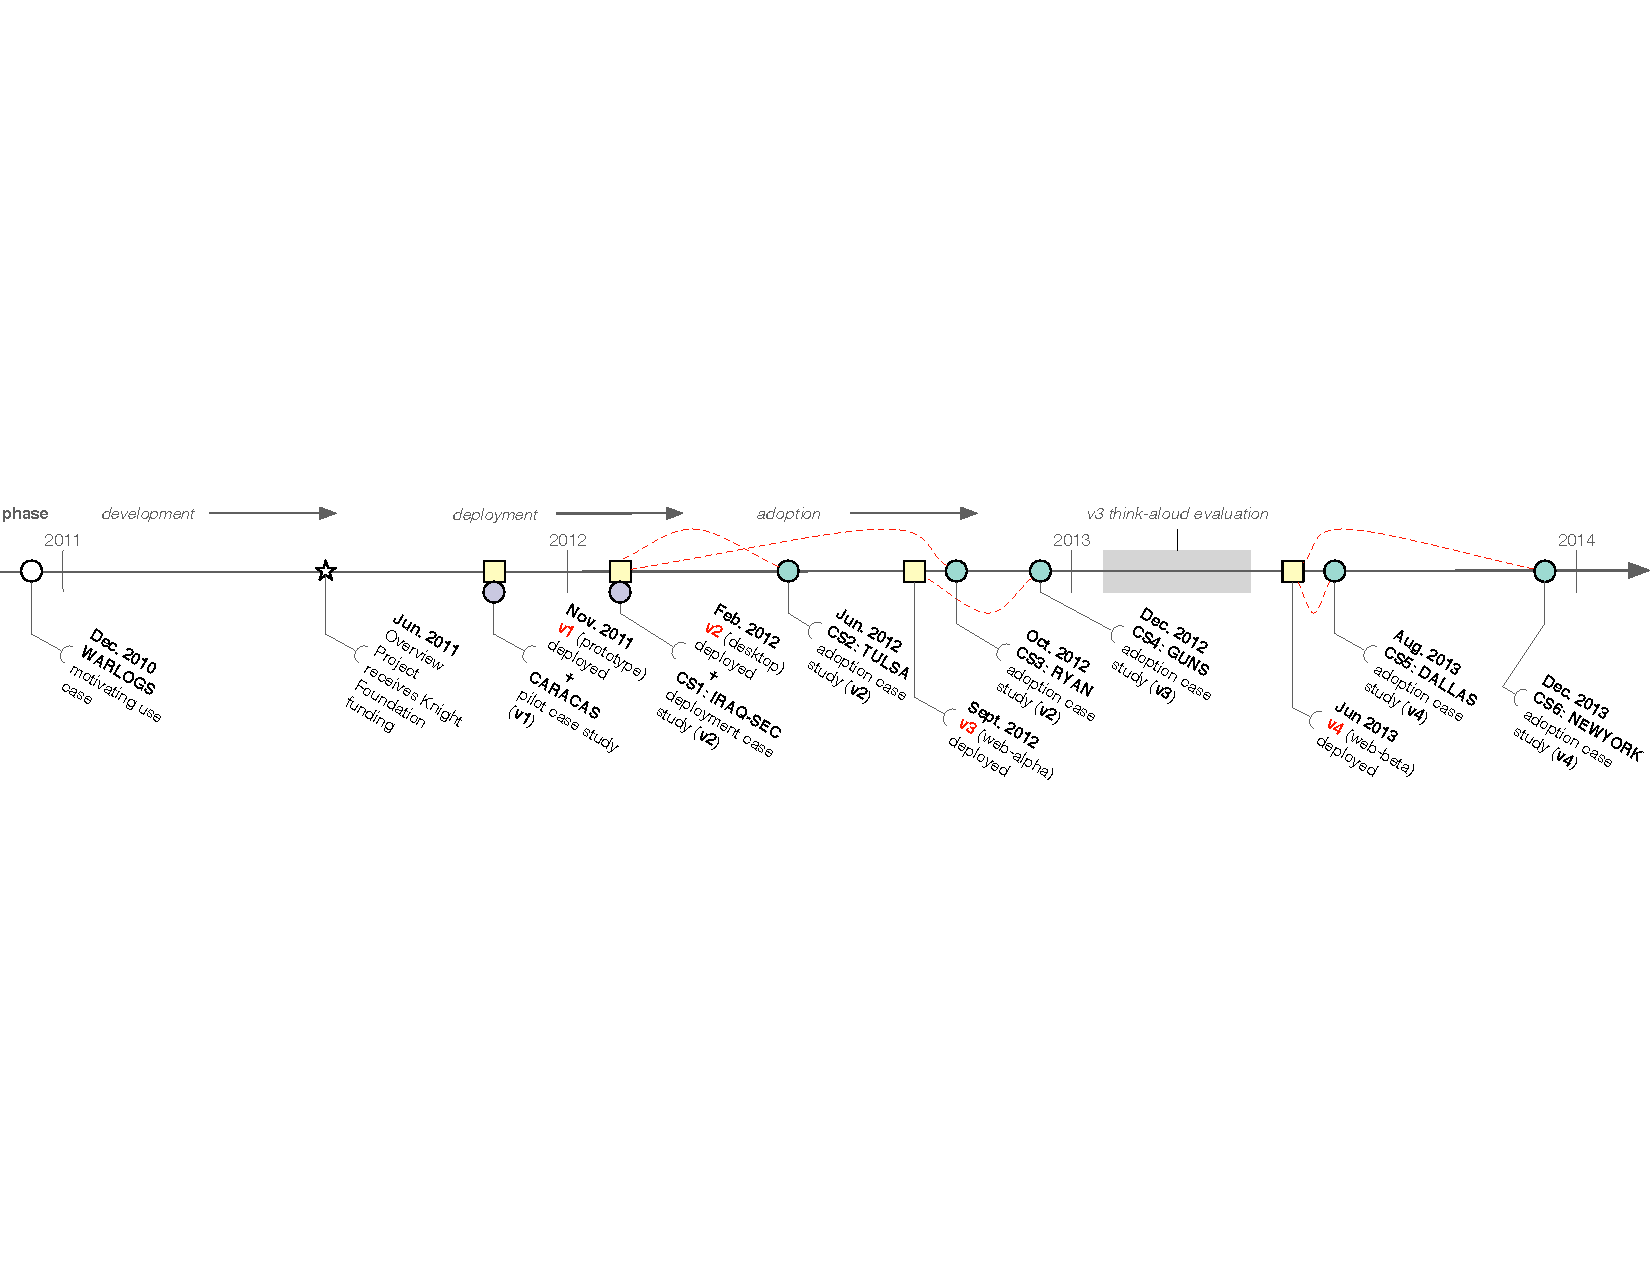
\includegraphics[width=0.975\textwidth]{figures/timeline.pdf}
	\caption
	[
	    A timeline of \textsl{Overview}'s development, deployment, and adoption phases.
	]
	{
	    A timeline of \textsl{Overview}'s development, deployment, and adoption phases: deployments are represented as yellow squares; deployment-phase case studies are represented as \raisebox{-.2\height}{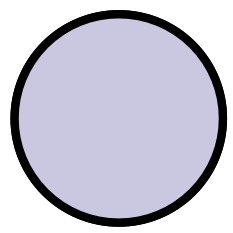
\includegraphics[width=0.015\textwidth, height=0.015\textwidth]{figures/deployment-case-study.png}} (purple circles), while adoption-phase case studies are represented as \raisebox{-.2\height}{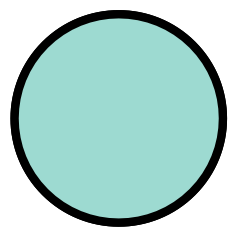
\includegraphics[width=0.015\textwidth, height=0.015\textwidth]{figures/adoption-case-study.png}} (turquoise circles).
	    The dotted red lines indicate which version of \textsl{Overview} was used in each case study.
	}
	\centering
	\label{overview:fig:timeline}
\end{figure}

%-|-|-|-|-|-|-|-|-|-|-|-|-|-|-|-|-|-|-|-|-|-|-|-|-|-|-|-|-|-|-|-|-|-|-|-|-

We frame this work as a visualization field study, one that took place during and after a process of iterative design addressing a particular domain problem, involving collaborators and people from that domain.
The contributions of this chapter include our classification of data\index{data abstraction} and task abstractions\index{task!task abstraction}, a description of its usage in real investigations spanning four deployments and six case studies\index{case study}, and a detailed analysis of the mapping from these abstractions\index{task!task abstraction} to visual encoding\index{visual encoding} and interaction\index{interaction} design choices.
This analysis led to important design revisions, based on a better understanding of {\it why}\index{{\tt why}} and {\it how}\index{{\tt how}} journalists\index{journalism} use {\it Overview}\index{Overview (document mining tool)}. 
From this experience we propose transferable lessons for visualization design methodology.

% The remainder of this chapter is organized as follows:
% We begin with a survey of related work in \autoref{overview:rw}.
% We then describe our initial use case in \autoref{overview:motivation}.
% The design of {\it Overview} is presented in \autoref{overview:overview}, which includes our initial task abstraction, {\it Overview}'s underlying data abstractions, and a description of its interface.
% In \autoref{overview:usage}, we report on real world usage of {\it Overview} by six journalists who used it for their own investigations; in five of these cases, the investigation resulted in a published story.
% Based on our observations of what these people did, we revisit our initial task abstraction and reflect upon the rationale for {\it Overview}'s visual encoding and interaction design choices in \autoref{overview:analysis}.
% Finally, in \autoref{overview:discussion}, we reflect on the methodological implications of our approach, and \autoref{overview:conclusion} summarizes our contributions.

%-------------------------------------------------------------------------
%-------------------------------------------------------------------------

\section{Related Work}
\label{overview:rw}

%-------------------------------------------------------------------------
%-------------------------------------------------------------------------

There have been a number of approaches and tools to support the analysis of document collections\index{document data}, spanning a range of data transformations and visual encodings\index{visual encoding}.  
We also review how these tools were evaluated\index{evaluation}.

\bstart{Topic model visualization}
One common approach to visualizing a document collection\index{document data} uses probabilistic topic models\index{topic models} inferred from the collection. 
These define topics as distributions of words and assign a distribution of topics per document. 
Both distributions are visualized directly in recent work by \citet{Chaney2012}, while other tools or techniques focus on the number of documents in each topic~\cite{Cui2011,Dou2013,Liu2012}, or use the topic assignments to compute the similarity between documents ~\cite{Chen2009,Eisenstein2012}. 
{\it Overview}\index{Overview (document mining tool)} does not use distribution-based topic models\index{topic models} but directly creates a hard hierarchical clustering\index{algorithms!clustering}, which is visually encoded as a tree\index{visual encoding!tree}.

\bstart{Documents as points}
Many visualization tools, including the first two versions of {\it Overview}\index{Overview (document mining tool)}, encode\index{{\tt encode}} individual documents as points in a scatterplot\index{visual encoding!scatterplot}. 
InfoSky~\cite{Granitzer2004} places points according to a pre-existing hierarchical arrangement\index{{\tt arrange}} of documents; in contrast, {\it Overview}\index{Overview (document mining tool)} is intended for document collections\index{document data} that do not have a pre-existing hierarchical structure\index{hierarchical data}. 
Other approaches begin with an unstructured document collection\index{document data} and place points based on document similarity metrics and \ac{DR}\index{dimensionality reduction (DR)} techniques, such as Leaksplorer~\cite{Leaksplorer}, PEx~\cite{Paulovich2007}, and EV~\cite{Chen2009}. 
{\it Overview v1-v2} included a similar scatterplot\index{visual encoding!scatterplot} which placed points by \ac{DR}\index{dimensionality reduction (DR)} through \ac{MDS}\index{dimensionality reduction (DR)!multi-dimensional scaling (MDS)}.
Finally, ForceSPIRE~\cite{Endert2012b} and TopicViz~\cite{Eisenstein2012} incorporate a scatterplot\index{visual encoding!scatterplot} where points corresponding to documents can be interactively placed according to one's own semantics or mental model, adaptively adjusting the underlying similarity metric used between document pairs.
In \autoref{overview:rationale}, we discuss in greater detail why a scatterplot\index{visual encoding!scatterplot} was omitted from later versions of {\it Overview}\index{Overview (document mining tool)}, and how tagging documents and clusters is an effective alternative to interactive placement.

\bstart{Documents as landscapes or clouds}
Document collections\index{document data} have also been encoded\index{{\tt encode}} as landscapes, three-dimensional visual encodings\index{visual encoding!scatterplot!3D scatterplot} of two- dimensional scatterplots\index{visual encoding!scatterplot} where height represents density, as in In-Spire~\cite{Hetzler2004} and recent work by \citet{Oesterling2011}.
However, empirical studies have shown that spatial landscapes are not well suited for encoding\index{{\tt encode}} inherently non-spatial data, and exhibit poor visual memory performance in comparison to two-dimensional scatterplots~\cite{Tory2009}\index{visual encoding!scatterplot}.

It is also possible to visualize a document collection\index{document data} by encoding\index{{\tt encode}} clusters of documents as interactive tag clouds\index{visual encoding!tag cloud}, as in Newdle~\cite{Liu2013}.
Once again, previous research has documented the perceptual drawbacks of tag clouds~\cite{Hearst2008}\index{visual encoding!tag cloud}.
By encoding\index{{\tt encode}} a document collection\index{document data} as a tree\index{visual encoding!tree}, {\it Overview}\index{Overview (document mining tool)} circumvents these issues.

\bstart{Documents as networks of entities}
Jigsaw's approach~\cite{Gorg2013,Kang2012} to document collection\index{document data} analysis differs from {\it Overview}\index{Overview (document mining tool)} in that it emphasizes the extraction of entities from documents, linking names, places, events, and dates, visualizing these relationships\index{network data}. 
The emphasis on entities is reflective of the domains in which Jigsaw is used, which include intelligence analysis\index{intelligence analysis}, law enforcement\index{law enforcement}, and academic research~\cite{Kang2012}.
Journalists\index{journalism} frequently start with barely-legible scanned documents which must first be converted to text through \ac{OCR}, greatly reducing the accuracy of standard entity extraction techniques.
As a flexible multiple-view application, Jigsaw also has a significant learning curve, and people have reported investing many months into learning how to use it~\cite{Kang2012}.
The journalists\index{journalism} we spoke to are accustomed to short deadlines and may only intermittently be working on a story involving a large document collection\index{document data}, so simplicity is a crucial requirement. 

\bstart{Documents as trees and rivers}
Like {\it Overview}\index{Overview (document mining tool)}, HierarchicalTopics~\cite{Dou2013} features a tree\index{visual encoding!tree} of document clusters\index{document data}, initially arranged\index{{\tt arrange}} by similar keywords.
It allows people to re-arrange\index{{\tt arrange}} the tree\index{visual encoding!tree} according to their own semantics, similar to how a person who uses ForceSPIRE can rearrange\index{{\tt arrange}} documents in a scatterplot~\cite{Endert2012b}\index{visual encoding!scatterplot}.
HierarchicalTopics~\cite{Dou2013} additionally allows people to track topic prevalence over time with a stacked area graph visual encoding in the style of a ThemeRiver~\cite{Havre2002}\index{visual encoding!stacked area graph}.
However, this approach requires temporal metadata that would be difficult to extract from the diverse document sources supported by {\it Overview}\index{Overview (document mining tool)}.

\bstart{Evaluating visual document mining tools}
Several of the aforementioned tools have been evaluated\index{evaluation} via controlled experiments and case studies\index{case study}.
Controlled experiments, such as those used to evaluate\index{evaluation} Newdle~\cite{Liu2013} or HierarchicalTopics~\cite{Dou2013}, often involve non-specialists conducting domain-agnostic tasks\index{task} specified by the researchers, who conjecture that they match with real world usage. 
Moreover, the documents used in these controlled experiments were collections of online news articles which are not appropriate test data for {\it Overview}\index{Overview (document mining tool)}, as professionally produced news articles are clean and homogeneous, unlike the diverse and messy documents obtained by our case study\index{case study} journalists\index{journalism}, which often contain little or no metadata; news articles are the output\index{{\tt output}} of the journalistic\index{journalism} document mining\index{document mining} process, not the input\index{{\tt input}}.

Most similar to our approach is a series of case studies\index{case study} of academic researchers, intelligence analysts\index{intelligence analysis}, and law enforcement\index{law enforcement} personnel who had adopted\index{adoption} Jigsaw~\cite{Kang2012}.
These case studies\index{case study} resulted in a better understanding of Jigsaw's utility in relation to the tasks\index{task} of people working in a specific application domain; like us, they identified similar barriers to adoption\index{adoption} and their results suggested new directions for design~\cite{Gorg2013,Gorg2014}.

%-------------------------------------------------------------------------
%-------------------------------------------------------------------------

\section{Initial Use Case}
\label{overview:motivation}

%-------------------------------------------------------------------------
%-------------------------------------------------------------------------

The {\it Overview}\index{Overview (document mining tool)} project began in December 2010, when journalist\index{journalism} and co-author Jonathan Stray visualized a subset (11,616 of 391,832) of the WikiLeaks Iraq War Logs~\cite{Stray2010}.
Journalists\index{journalism} had previously examined these documents by using text search to retrieve specific records and by visualizing the structured data fields such as time and location, but they had not attempted an analysis of the unstructured text of the reports.
In this initial use case, which we will refer to as {\sc warlogs}, documents were visualized as points placed according to a measure of similarity between documents and coloured according to pre-existing categorical labels, such as {\it ``friendly action''} and {\it ``criminal incident.''}  As shown in \autoref{overview:fig:warlogs}, this design revealed meaningful cluster structure that cross-cuts the colourings, showing that the pre-existing coarse categorization does not capture the whole story\footnote{The entire image is shown in \autoref{app:overview:initial-use-case}.}.

%-|-|-|-|-|-|-|-|-|-|-|-|-|-|-|-|-|-|-|-|-|-|-|-|-|-|-|-|-|-|-|-|-|-|-|-|-

\begin{figure}
	\centering
	\fbox{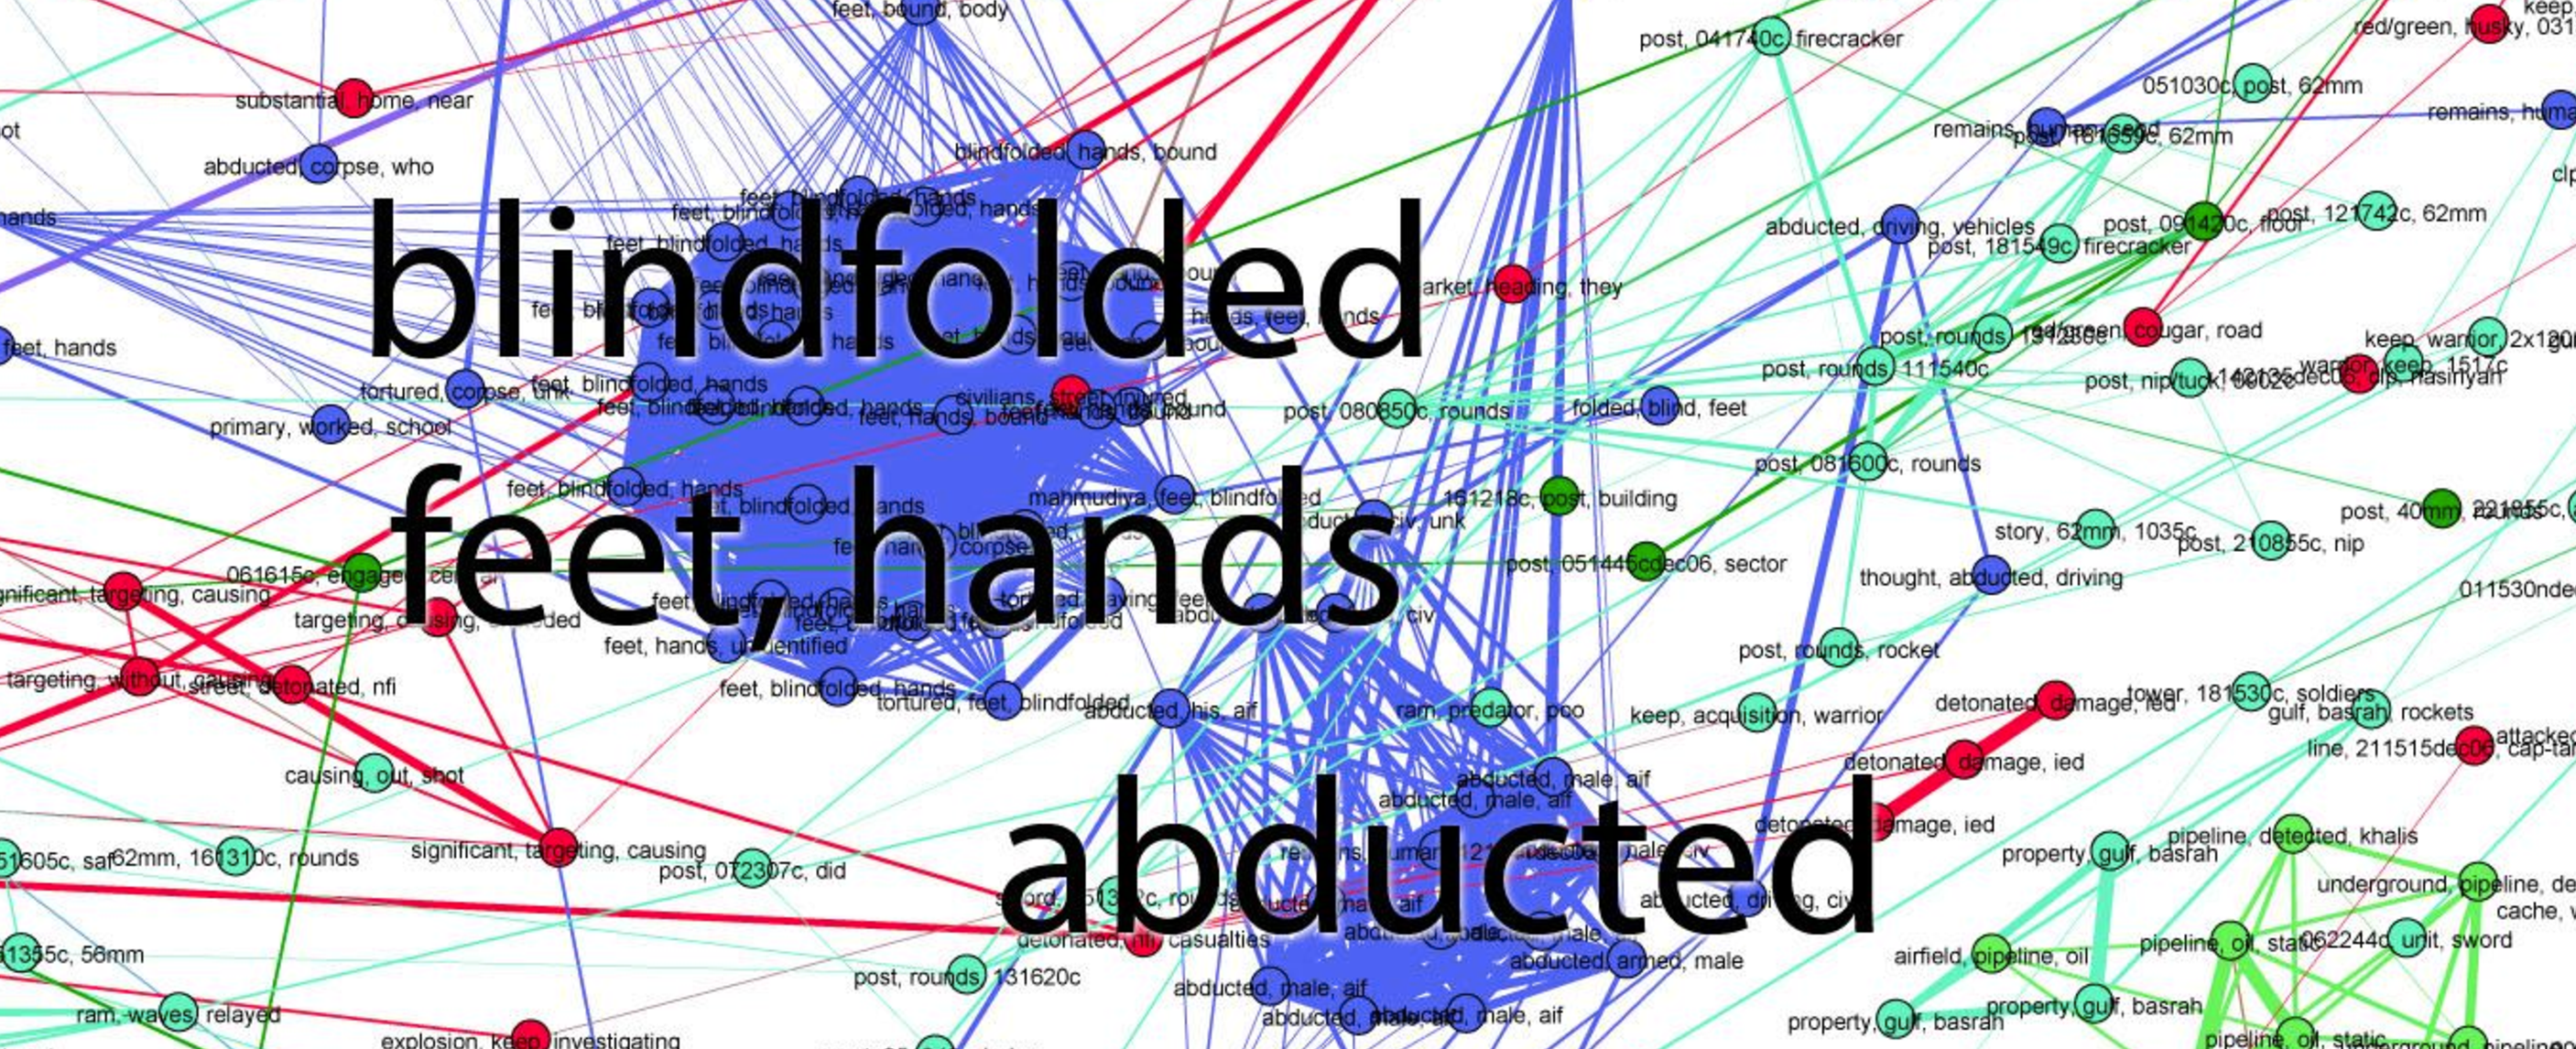
\includegraphics[width=0.975\textwidth]{figures/warlogs.pdf}}
	\caption
	[
	    Detail from \textsl{``A full-text visualization of the Iraq War Logs''}.
	]
	{
	    Detail from \textsl{``A full-text visualization of the Iraq War Logs''} ({\sc warlogs})~\cite{Stray2010}, in which distinct clusters of documents are visible; these documents pertain to ``criminal incidents'' during the Iraqi civil war involving abductions and blindfolding.
	}
	\centering
	\label{overview:fig:warlogs}
\end{figure}

%-|-|-|-|-|-|-|-|-|-|-|-|-|-|-|-|-|-|-|-|-|-|-|-|-|-|-|-|-|-|-|-|-|-|-|-|-

The {\sc warlogs} scatterplot\index{visual encoding!scatterplot} had serious limitations: it was not possible to interactively and systematically examine the contents of clusters of documents.
However, it demonstrated that visual cluster analysis could illuminate previously unknown and meaningful structure in a real world document collection\index{document data}, a conjecture that Stray had synthesized from his previous experience reporting on this collection of documents.
On the basis of this promising result, Stray collaborated with us to design an interactive visualization tool for document mining\index{document mining}.

%-------------------------------------------------------------------------
%-------------------------------------------------------------------------

\section{Design of Overview}
\label{overview:overview}

%-------------------------------------------------------------------------
%-------------------------------------------------------------------------

We now describe our initial task abstraction\index{task!task abstraction}, {\it Overview}'s\index{Overview (document mining tool)} underlying data abstractions, and the elements of its interface.

\bstart{Initial task abstraction}
During the development of {\it Overview v1-v2}, our task abstraction\index{task!task abstraction} was based on the {\sc warlogs} use case: journalists\index{journalism} would be motivated by the hypothesis that their document collection\index{document data} contained a semantically interesting cluster structure, and would require a means\index{task!means} for {\tt exploring}\index{{\tt explore}} that structure, drilling down into these clusters to examine the contained documents.
During this exploration\index{{\tt explore}}, they would need a way to keep track of what they had discovered, allowing them to revisit previously examined clusters and documents.

\bstart{Data abstractions}
Although {\it Overview}'s\index{Overview (document mining tool)} design has evolved over the course of four deployed versions, it continues to reflect several underlying data abstractions\index{data abstraction}.
{\it Overview}\index{Overview (document mining tool)} does not incorporate any novel text analysis\index{information retrieval} techniques; following a practice common in that domain, we convert each document to a vector of words weighted by the \ac{TF-IDF}\index{term frequency-inverse document frequency (TF-IDF)} formula, and compute similarity between documents using the cosine distance metric~\cite{Salton1988}.
We generate our document clusters\index{document data} by hierarchically clustering\index{algorithms!clustering} these distances and encoding\index{{\tt encode}} the result as a tree~\cite{Ingram2013,Ingram2012}\index{visual encoding!tree}.
Clusters are labeled with keywords extracted via \ac{TF-IDF}\index{term frequency-inverse document frequency (TF-IDF)} scores.

Multiple meaningful clusterings may exist for any collection of documents~\cite{Grimmer2011}; our particular distance metric and hierarchical clustering algorithm\index{algorithms!clustering} is but one possible choice.
Human-generated clusterings that leverage domain knowledge can complement automatic clusterings~\cite{Dou2013,Endert2012b}.
For these reasons, {\it Overview}\index{Overview (document mining tool)} allows for an arbitrary number of human-generated {\it tags} on each document, which can be assigned to individual documents or at the cluster level.
Tags allow people to keep track of what they have found and where they have looked so far.

%-|-|-|-|-|-|-|-|-|-|-|-|-|-|-|-|-|-|-|-|-|-|-|-|-|-|-|-|-|-|-|-|-|-|-|-|-

\begin{figure}
	\centering
	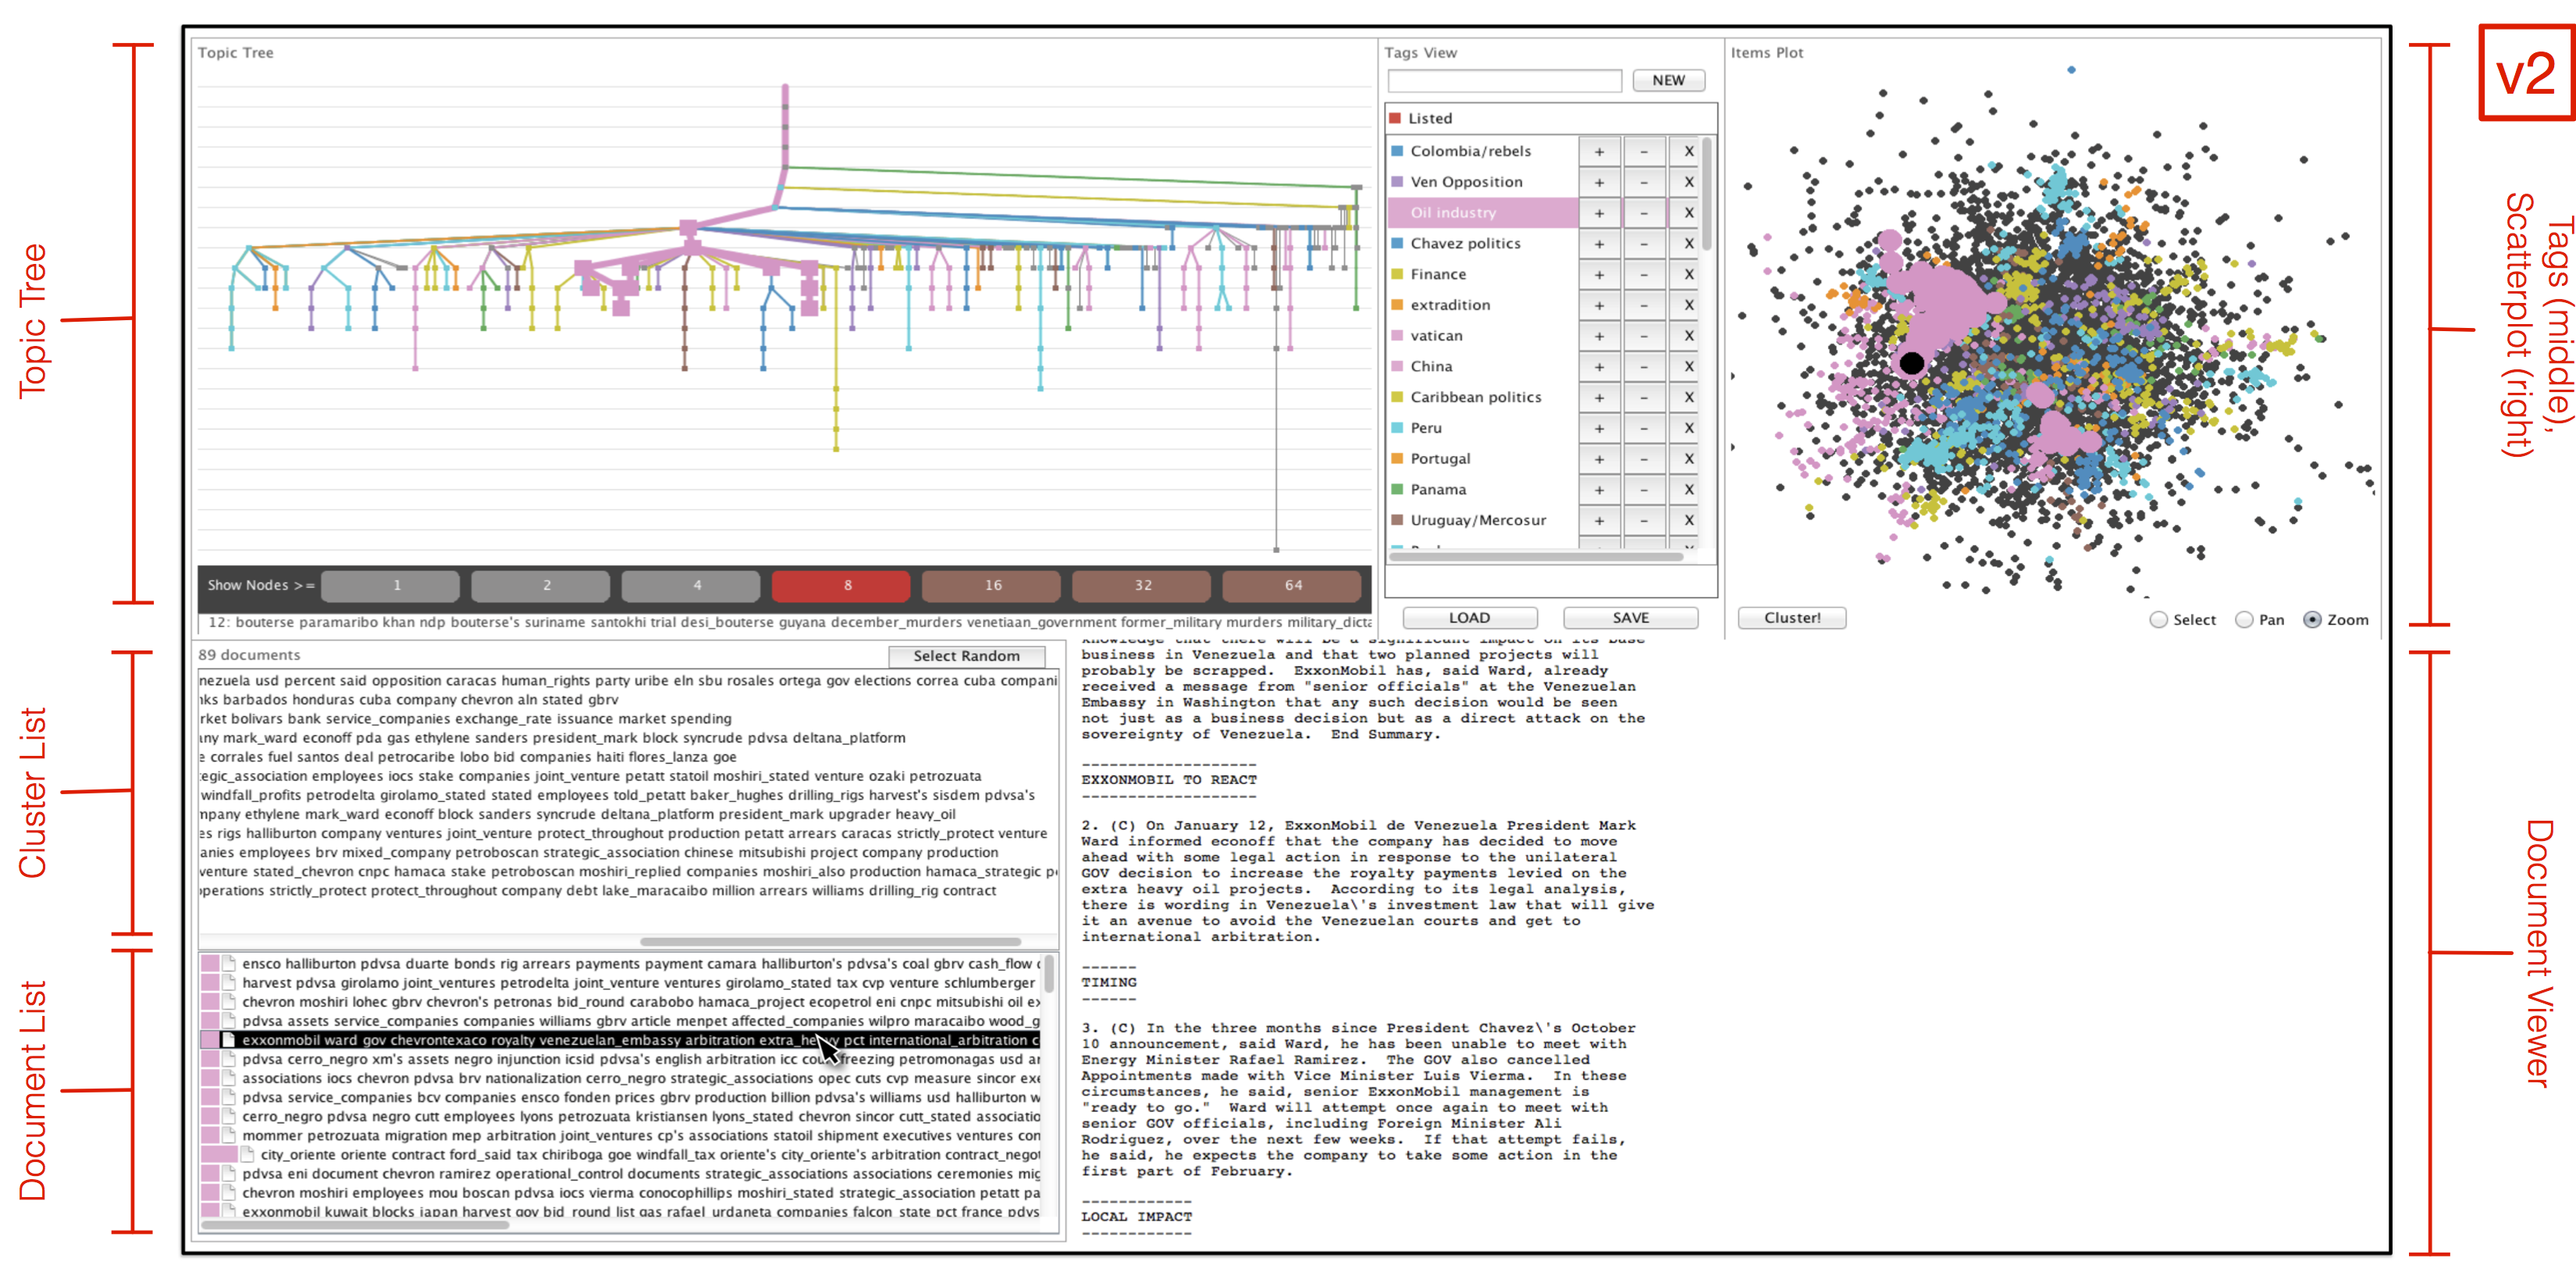
\includegraphics[width=\textwidth]{figures/overview-v2-annotated.png}
	\caption
	[
	    \textsl{Overview v2}, a desktop application released in Winter 2012.
	]
	{
    	\textsl{Overview v2}, a desktop application released in Winter 2012.
    	Shown here is 6,849 of the U.S. State Department diplomatic cables released by WikiLeaks, those pertaining to Venezuela.
    	The \textsl{``Oil industry''} tag is {\tt selected}; clusters containing documents having this tag are emphasized in pink in the \textsl{Topic Tree} and are shown in the \textsl{Cluster List} as a set of keywords.
    	Individual documents having the \textsl{``Oil industry''} tag are emphasized in the scatterplot and shown in the \textsl{Document List} as a set of keywords.
    	The fifth document is {\tt selected}; its contents are displayed in the \textsl{Document Viewer} and it is marked as a larger black dot in the scatterplot.
	}
	\centering
	\label{overview:fig:overview-v2}
\end{figure}

%-|-|-|-|-|-|-|-|-|-|-|-|-|-|-|-|-|-|-|-|-|-|-|-|-|-|-|-|-|-|-|-|-|-|-|-|-

%-|-|-|-|-|-|-|-|-|-|-|-|-|-|-|-|-|-|-|-|-|-|-|-|-|-|-|-|-|-|-|-|-|-|-|-|-

\begin{figure}
	\centering
	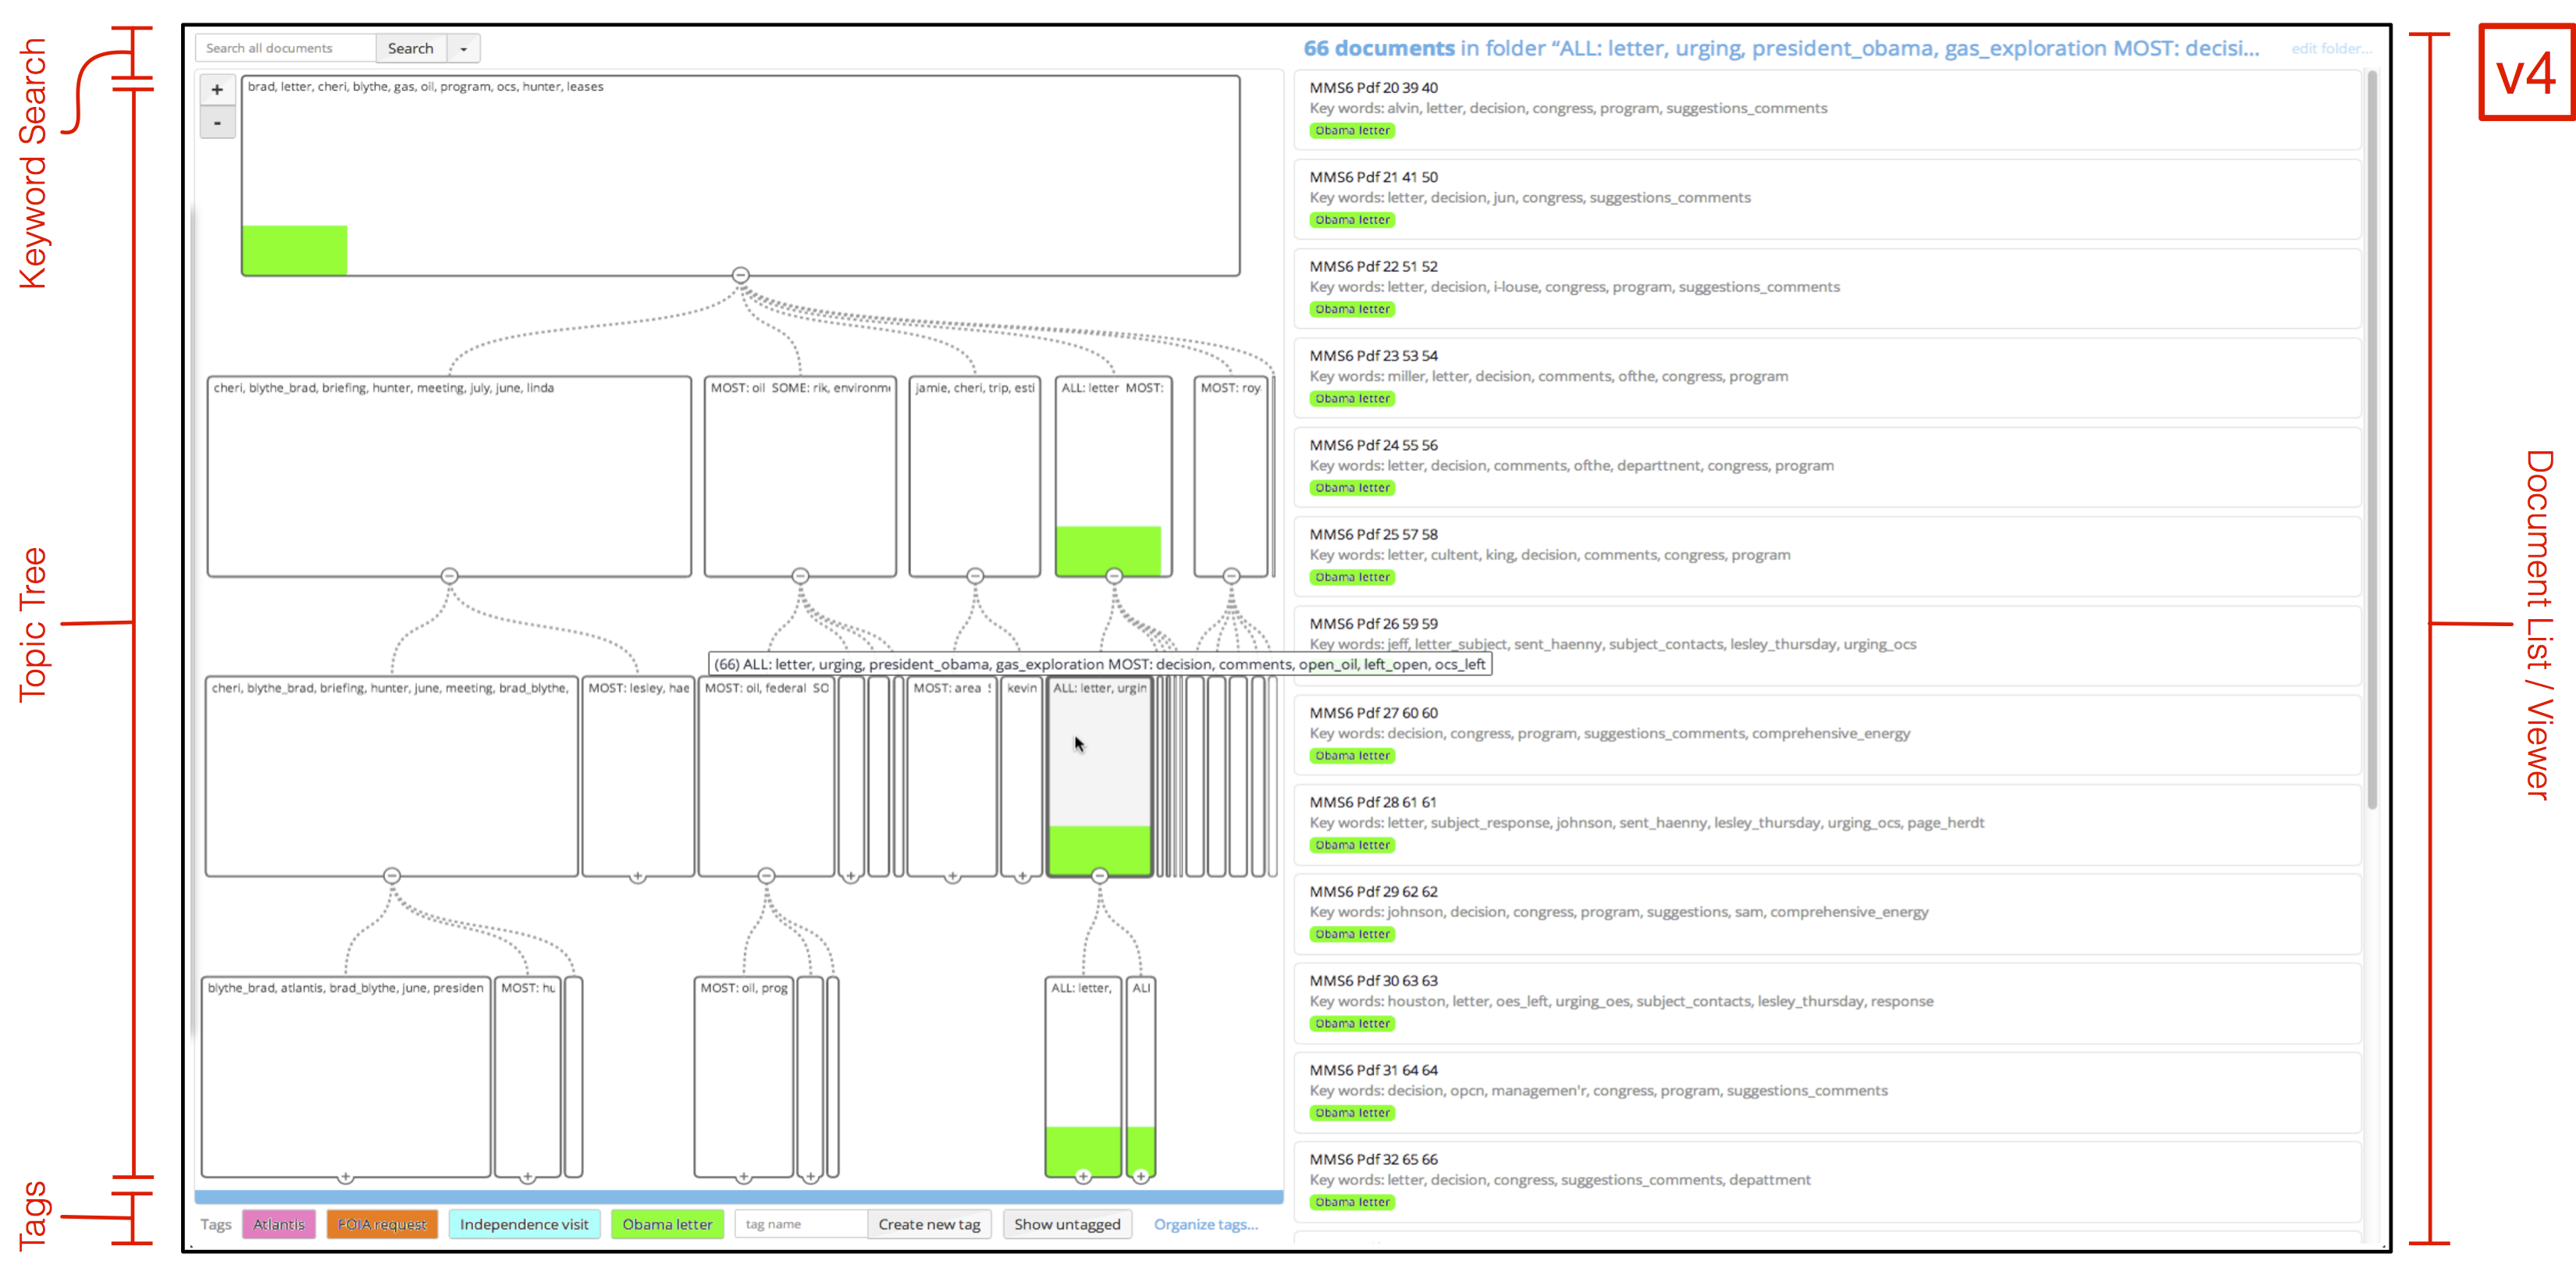
\includegraphics[width=\textwidth]{figures/overview-v4-annotated.png}
	\caption
	[
	    \textsl{Overview v4}, a web-based application released in Summer 2013.
	]
	{
    	\textsl{Overview v4}, a web-based application released in Summer 2013.
    	Shown here is 625 White House email messages concerning drilling in the Gulf of Mexico prior to the 2010 Deepwater Horizon oil spill.
    	The \textsl{``Obama letter''} tag is {\tt selected}; clusters containing documents having this tag are highlighted in green in the \textsl{Topic Tree}.
    	One of these clusters is {\tt selected} and its keywords are displayed in a tooltip; the 66 documents in this cluster are listed in the \textsl{Document List}. 
    	{\tt Selecting} a document from this list reveals the \textsl{Document Viewer} (cf. \autoref{overview:fig:overview-v4-teaser}).
	}
	\centering
	\label{overview:fig:overview-v4}
\end{figure}

%-|-|-|-|-|-|-|-|-|-|-|-|-|-|-|-|-|-|-|-|-|-|-|-|-|-|-|-|-|-|-|-|-|-|-|-|-

\bstart{Interface}
With each deployment came changes to the interface, though we will focus on the differences between {\it Overview v2} and {\it v4}, shown in \autoref{overview:fig:overview-v2} and~\ref{overview:fig:overview-v4}\footnote{A video demonstration of {\it Overview v4} is available here: \url{http://vimeo.com/71483614}.}, respectively.
The visualization design of {\it v1} and {\it v2} are quite similar to each other, as are {\it v3} and {\it v4}\footnote{Screenshots of {\it v1} and {\it v3} can be found in \autoref{app:overview} as \autoref{app:overview:fig:overview-v1} and \autoref{app:overview:fig:overview-v3}, respectively.}.  

Common to all deployed versions of {\it Overview}\index{Overview (document mining tool)} is the {\it Topic Tree}\index{visual encoding!tree} visual encoding\index{visual encoding}, representing a hierarchical clustering\index{algorithms!clustering} of similar documents\index{document data}, the {\it Document List}, showing currently {\tt selected}\index{{\tt select}} documents, the {\it Document Viewer}, and the ability to create and assign custom categorical tags to clusters or individual documents; tags are {\tt encoded}\index{{\tt encode}} as coloured labels on documents and clusters.
{\tt Selections}\index{{\tt select}} of documents are propagated and highlighted across views\index{view coordination!brushing across views}.

The {\it Topic Tree}\index{visual encoding!tree} underwent some of the most significant changes. 
It was redesigned to emphasize nodes, and to {\tt encode}\index{{\tt encode}} the number of documents in each node, instead of focusing on the edges between identically-sized nodes.
In {\it v1-v2}, the {\it Topic Tree}\index{visual encoding!tree} could be pruned based on a threshold cluster size, controlled using a set of coloured radio buttons below; in {\it v3}, we replaced threshold pruning with an open/close interface that allows a person to show or hide the children of any node.
Pan and zoom controls were also added, including an auto-zoom feature that automatically zooms and pans to a selected node.

Another prominent change was the removal of the interactive scatterplot\index{visual encoding!scatterplot}, in which individual documents were {\tt encoded}\index{{\tt encode}} by points and their placement corresponded to a two-dimensional projection of the original high-dimensional\index{high-dimensional data} \ac{TF-IDF}\index{term frequency-inverse document frequency (TF-IDF)} vector space, generated via \ac{MDS}\index{dimensionality reduction (DR)!multi-dimensional scaling (MDS)}; pairs of documents appearing closer together were deemed to be more similar than pairs of documents that were farther apart. 
The scatterplot\index{visual encoding!scatterplot} had panning and zooming controls, and document-points could be {\tt selected}\index{{\tt select}} via clicking or lassoing.

We also removed the {\it Cluster List} and consolidated the {\it Document Viewer} with the {\it Document List} (\cf \autoref{overview:fig:overview-v4-teaser}).
The {\it Document List} now displays the document title, extracted keywords, and coloured labels indicating which tags have been applied to each document.
We added full-text keyword search in {\it v4}; documents matching a search term are highlighted with colour labels in the {\it Topic Tree}\index{visual encoding!tree}, and these results can be saved as a persistent tag.
Finally, we added a {\it ``Show Untagged''} button in {\it v4}, which highlights documents and clusters where no tags have been applied, a crucial feature for the (initially unexpected) task\index{task} of exhaustively reviewing a document collection\index{document data}.

This section described the design without providing any rationale for its evolution. 
Our decisions were based on observations of real world usage; we provide concrete examples of {\it why}\index{{\tt why}} and {\it how}\index{{\tt how}} {\it Overview}\index{Overview (document mining tool)} was used by journalists\index{journalism} in \autoref{overview:usage}. 
Then, in \autoref{overview:analysis}, we present our final task abstraction\index{task!task abstraction}, the outcome of analyzing these observations, and justify our design choices with respect to these revisited tasks\index{task}. 

%-------------------------------------------------------------------------
%-------------------------------------------------------------------------

\section{Observations of Real World Usage}
\label{overview:usage}

%-------------------------------------------------------------------------
%-------------------------------------------------------------------------

We conducted six case studies\index{case study} where we analyzed the use of {\it Overview}\index{Overview (document mining tool)} by investigative journalists\index{journalism}.
We distinguish between a {\it case study}\index{case study} and a {\it usage scenario}~\cite{Sedlmair2012}\index{usage scenario}, in which the former involves a person from the target application domain who uses a tool to examine their own data, having goals related to their ongoing work; in contrast, the latter reports usage of a tool by its designers with curated data and conjectured tasks\index{task}.

\bqstart{Pilot case study}:
The first person who used {\it Overview}\index{Overview (document mining tool)} was the Associated Press Caracas bureau chief, whom we asked in November 2011 to use the {\it v1} prototype to examine 6,849 of the 251,287 U.S. State Department diplomatic cables released by WikiLeaks, those pertaining to Venezuela; this document collection\index{document data} is featured in \autoref{overview:fig:overview-v2}.
Although he found the tool to be interesting, his analysis did not lead to a published story.
This informal pilot case study\index{case study} revealed basic usability problems and the experience prompted us to formalize the case study\index{case study} process and determine foci of interest, such as utility, usability, learnability, and journalists'\index{journalism} tasks\index{task} in context.

\bstart{Metrics}
In addition to the qualitative analysis of journalists'\index{journalism} tasks\index{task}, we also focus on the metric of adoption\index{adoption} defined as {\it self-initiated} use: did a journalist\index{journalism} freely chose to use the tool for their own investigation, rather than trying out the tool in response to direct solicitation by the researchers?
According to this distinction, adoption\index{adoption} occurred in five of the six case studies\index{case study} we report, as indicated by the turquoise circles in \autoref{overview:fig:timeline}; the journalist\index{journalism} in the remaining case study\index{case study} ({\sc iraq-sec}) was co-author Stray.
We were also interested in the outcome of a journalist's\index{journalism} investigation: did they complete their investigation to satisfaction
as a result of using {\it Overview}\index{Overview (document mining tool)}, either by choosing to publish a story or by deciding that their findings did not merit a story? Or did they abandon {\it Overview}\index{Overview (document mining tool)} because the tool did not help further their investigation?

\begin{sloppypar}
\bstart{Recruitment}
Since the {\it v2} deployment, Stray has promoted {\it Overview}\index{Overview (document mining tool)} within the data journalism\index{journalism} community.
Several hundred journalists\index{journalism} have created accounts on the public server, and they have collectively uploaded more than nine million documents; {\it Overview}\index{Overview (document mining tool)} is used by approximately two hundred unique people each month\footnote{As of March 2014.}. 
As of \today, we are aware of twenty published stories where {\it Overview}\index{Overview (document mining tool)} played a part in the investigative process\footnote{Links to these stories can be found here: \url{https://github.com/overview/overview-server/wiki/News-stories}. A blog post that summarizes several of these stories is available here: \url{https://blog.overviewdocs.com/completed-stories/}}, five of which are discussed as case studies\index{case study} below.
The self-initiated journalists\index{journalism} featured in case studies\index{case study} 2--6 were recruited to participate in our study after they contacted Stray with technical questions, which often pertained to workflow\index{workflows} difficulties such as wrangling their document collection\index{document data} into a format that {\it Overview}\index{Overview (document mining tool)} could ingest.
\end{sloppypar}

\bstart{Methods}
Our case study\index{case study} findings are the result of triangulating between multiple data collection and analysis methods\footnote{\autoref{app:overview:proposal} provides additional detail regarding our data collection and analysis methodology.}.
Our primary data collection method was that of a semi-structured interview\footnote{Our interview protocol is provided in \autoref{app:overview:interview-protocol}.}.
We conducted interviews via Skype or Google$^+$ Hangout, as our journalists\index{journalism} were geographically remote; both services include a screen sharing feature, allowing journalists\index{journalism} to demonstrate aspects of their investigative process.
We recorded these interviews and demonstrations using a screen capture application and later transcribed them.
The deadline-driven nature of journalism\index{journalism} precluded multiple interviews during an ongoing investigation, so we chose to interview each journalist\index{journalism} after their investigation was complete, despite the known limitations of retrospective introspection~\cite{Ericsson1980}.
Journalists\index{journalism} were encouraged but not expected to keep a diary relating to their ongoing use of {\it Overview}\index{Overview (document mining tool)}.
Five of our case study\index{case study} journalists\index{journalism} wrote or contributed to retrospective blog posts about their process~\cite{Keller2012a,Stray2012a,Stray2012b,Stray2014,Wade2012a}, and one of them ({\sc tulsa}) also sent us his personal notes.

We also collected usage logs for each journalist\index{journalism}, consisting of timestamped interactions with {\it Overview}\index{Overview (document mining tool)}, which included {\tt selecting}\index{{\tt select}}, viewing, and {\tt annotating}\index{{\tt annotate}} documents and clusters with tags.
Log file\index{interaction!interaction logs} analysis allowed us to partially reconstruct a journalist's\index{journalism} analysis process, complementing information divulged to us in their retrospective interview.
Finally, each journalist\index{journalism} provided us with their tagged document collection\index{document data}, which helped to establish a shared context.

%-------------------------------------------------------------------------

\subsection{Case Studies}
\label{overview:case-studies}

%-------------------------------------------------------------------------


The six case studies\index{case study} we present, summarized in \autoref{overview:tab:case-studies}, took place between February 2012 and December 2013, as indicated in \autoref{overview:fig:timeline}.

\bscstart{CS1: IRAQ-SEQ~\cite{Stray2012}}
Our first case study\index{case study} took place in February 2012, when journalist\index{journalism} and co-author Stray  used {\it Overview v2} to analyze recently declassified documents from the Iraq war concerning the behavior of private security contractors.
In particular, he wanted to categorize and count types of documented incidents involving these contractors; aside from the high-profile incidents that made headlines, he wanted to determine the prevalence of other incidents that these contractors were involved in during the Iraq war.

The document collection\index{document data} was the result of a \ac{FOIA} request to the U.S. State Department, comprised of 666 incident reports over 4,500 pages, which were scanned using \ac{OCR}.
After the documents were loaded in {\it Overview}\index{Overview (document mining tool)}, Stray examined document clusters over the course of five days: he {\tt navigated}\index{{\tt navigate}} the {\it Topic Tree}\index{visual encoding!tree}, {\tt selected}\index{{\tt select}} clusters and their documents, {\tt aggregated}\index{{\tt aggregate}} clusters using the tree pruning controls, and {\tt annotated}\index{{\tt annotate}} approximately 48\% of the documents with 28 unique tags.
After a lengthy ``orientation'' phase to determine incident categories of interest, he sampled the documents using the ``Select Random'' button (above the {\it Cluster List} in \autoref{overview:fig:overview-v2}), which would {\tt select}\index{{\tt select}} a document from the {\it Document List} to be shown in the {\it Document Viewer}.
With this approach, he read and tagged 50 of the 666 reports, which allowed him to develop hypotheses regarding the prevalence of certain incident types.
Afterward, he followed up with U.S. State Department representatives, who provided additional context and a timeline for these incidents.
His published story~\cite{Stray2012} combines his categorical summarization with the context of the war.

\bscstart{CS2: TULSA~\cite{Wade2012}}
The first case of self-initiated adoption\index{adoption} by a journalist\index{journalism} took place in June 2012\footnote{Additional analysis of this case study is provided in \autoref{app:overview:proposal}.}, revealing a different motivation for using {\it Overview}\index{Overview (document mining tool)}.
In this case, the journalist\index{journalism} wanted to {\tt locate}\index{{\tt locate}} and {\tt identify}\index{{\tt identify}} evidence, documents that would support or refute a pre-existing hypothesis: he was following-up on an anonymous tip regarding municipal government mismanagement and potential conflicts of interest between city hall, municipal police, and police equipment vendors.
He filed a \ac{FOIA} request with the City Hall of Tulsa, Oklahoma for email messages between these organizations, and then used {\it Overview v2} to examine 5,996 of these email messages.

His search for corroborating evidence spanned multiple sessions over 18 days, beginning with an exhaustive and systematic left-to-right {\tt navigation}\index{{\tt navigate}} of the {\it Topic Tree}\index{visual encoding!tree}, {\tt aggregating}\index{{\tt aggregate}} clusters using the tree pruning controls, and {\tt selecting}\index{{\tt select}} clusters to view their contained documents.
He viewed roughly 70\% of the documents in the {\it Document Viewer} at least once, {\tt annotating}\index{{\tt annotate}} 92\% of them with 22 unique tags.
We observed that he undertook multiple iterations of tagging: he began by tagging entire clusters using terms appearing in cluster keywords, but later tagged individual documents throughout the tree\index{visual encoding!tree} with tags such as {\it ``important''}, {\it ``weird''}, and {\it ``follow-up.''}
As a result of this thorough tagging, the journalist\index{journalism} was able to {\tt lookup}\index{{\tt lookup}} and {\tt browse}\index{{\tt browse}} previously identified\index{{\tt identify}} clusters or documents of interest, focus on documents {\tt annotated}\index{{\tt annotate}} by multiple tags, or {\tt locate}\index{{\tt locate}} documents that remained untagged; the latter was accomplished by {\tt selecting}\index{{\tt select}} uncoloured points in the scatterplot\index{visual encoding!scatterplot}.
These tags also provided a starting point for the further {\tt annotation}\index{{\tt annotate}} of 129 {\it ``important''} documents with notes relating to his hypothesis; these notes eventually became integral parts of his published story~\cite{Wade2012}.

\bscstart{CS3: RYAN~\cite{Gillum2012}}
In October 2012, {\it Overview v2} was used yet again to {\tt locate}\index{{\tt locate}} evidence in support of a hypothesis, though there are several differences as compared to the {\sc tulsa} case study\index{case study}.
In this case, a journalist\index{journalism} wanted to follow-up on an earlier story and on accusations made by Vice President Joe Biden that vice-presidential nominee Paul Ryan's campaign statements were hypocritical.
In order to support or refute this hypothesis, the journalist\index{journalism} sought to {\tt compare} Ryan's campaign statements regarding wasteful government programs to his correspondence with various federal agencies concerning these same programs.
After filing over 200 \ac{FOIA} requests to these agencies, the journalist\index{journalism} received 8,680 pages of correspondence.
These physical documents arrived in several batches, and were scanned using \ac{OCR}.

The journalist\index{journalism} wanted to find genuine correspondence signed by Ryan; however, prevalent \ac{OCR} errors prevented him from {\tt locating}\index{{\tt locate}} these documents using keyword search. 
{\it Overview}\index{Overview (document mining tool)} was able to cluster documents effectively on the remaining intact text, and most of the documents in this collection were quickly found to be irrelevant to his hypothesis.
Over the course of half a day, he {\tt navigated}\index{{\tt navigate}} the {\it Topic Tree}\index{visual encoding!tree} to {\tt locate}\index{{\tt locate}} and {\tt identify}\index{{\tt identify}} a small subset of clusters containing one hundred and seventy-six pages of genuine correspondence containing Ryan's signature; the remainder could be safely ignored, comprised of attachments and other irrelevant correspondence.
Unlike the {\sc tulsa} journalist\index{journalism}, the {\sc ryan} journalist\index{journalism} {\tt annotated}\index{{\tt annotate}} a mere 8\% percent of the document collection\index{document data} with 12 unique tags.
As with {\sc tulsa}, the {\sc ryan} journalist\index{journalism} used tags as a starting point for the further {\tt annotation}\index{{\tt annotate}} of his source documents with notes; his published story~\cite{Gillum2012} compares these findings to Ryan's campaign statements.

\bscstart{CS4: GUNS~\cite{Keller2012}}
The first documented adoption\index{adoption} of {\it Overview}'s\index{Overview (document mining tool)} web application deployment ({\it v3}) took place in December 2012.
Shortly after the Newtown school shooting, the journalist\index{journalism} asked {\it Daily Beast} readers to self-identify as gun owners or non-owners, to report where they lived, and to post their opinion on the debate over gun ownership on a discussion board. 
He collected 1,278 comments: 757 from gun owners and 521 from non-owners.
He aimed to determine what the debate on gun ownership is about: do gun owners and non-owners raise the same issues? 
He was also curious about geographical differences.

He uploaded the responses from gun owners and non-owners into two separate instances of {\it Overview}\index{Overview (document mining tool)}.
Like the {\sc iraq-sec} case study\index{case study}, the {\sc guns} journalist\index{journalism} was interested in {\tt summarizing}\index{{\tt summarize}} a document collection\index{document data}, though the form of this {\tt summarization}\index{{\tt summarize}} was different. 
In {\sc iraq-sec}, the journalist\index{journalism} wanted to categorize and count types of documented incidents; in contrast, the {\sc guns} journalist\index{journalism} sought to {\tt identify}\index{{\tt identify}} documents that were representative of their clusters, the sensational and polarizing speaking points from both sides of the debate over gun ownership; he was less interested in a fine-grained classification or quantification.
For both sets of documents, he {\tt navigated}\index{{\tt navigate}} and {\tt selected}\index{{\tt select}} clusters and their contained documents, {\tt compared}\index{{\tt compare}} related clusters between the {\it gun owner} and {\it non-owner} instances, and later {\tt browsed}\index{{\tt browse}} previously identified clusters to {\tt identify}\index{{\tt identify}} representative quotes from people on both sides.
Ultimately, he read nearly all the discussion board comments over the course of a day.
Unlike the previous case studies\index{case study}, he did not use {\it Overview}'s\index{Overview (document mining tool)} tagging functionality, instead opting to copy quotes into an Excel\index{Excel (Microsoft)} spreadsheet, where he integrated geographical metadata and iteratively arranged\index{{\tt arrange}} quotes to construct a narrative for his story~\cite{Keller2012}.

\bscstart{CS5: DALLAS}
In August 2013, a journalist\index{journalism} used {\it Overview v4} in a similar fashion to that of the {\sc tulsa} journalist\index{journalism}, though the outcome of their investigations differed. 
In the {\sc dallas} case study\index{case study}, the journalist\index{journalism} had recently reported on a collection of 4,653 email messages resulting from a \ac{FOIA} request regarding the state government's response to an emergency incident.
The journalist\index{journalism} believed that some remaining evidence was left to be {\tt located}\index{{\tt locate}}, beyond what had already been reported in the earlier story.
Despite having already read all the documents in the collection (unassisted by {\it Overview}), the journalist\index{journalism} used {\it Overview}\index{Overview (document mining tool)} to verify that nothing was overlooked and sought to gather material for a follow-up story.
She subsequently used {\it Overview}\index{Overview (document mining tool)} to examine four additional collections of messages, analyzed individually, ranging in size between 1,858 and 3,564 email messages.

The keyword search feature introduced in {\it Overview v4} was found to be particularly useful: the journalist\index{journalism} alternated between {\tt identifying}\index{{\tt identify}} clusters by {\tt navigating}\index{{\tt navigate}}, {\tt aggregating}\index{{\tt aggregate}}, and {\tt selecting}\index{{\tt select}} nodes in the {\it Topic Tree}\index{visual encoding!tree}, and {\tt locating}\index{{\tt locate}} documents via keyword search, then {\tt identifying}\index{{\tt identify}} related documents.
As her analysis progressed, we observed that the journalist\index{journalism} relied more upon keyword search to highlight clusters of interest within the {\it Topic Tree}\index{visual encoding!tree}.
She applied tags to each of the five document collection\index{document data}s: the number of tags ranged between three and seven, and between 7\% and 52\% of documents were {\tt annotated}\index{{\tt annotate}} with at least one tag; in total, 14 out of 31 tags were created from keyword search results.

In this case, {\it Overview}\index{Overview (document mining tool)} was used to make the decision {\it not} to publish: after 12 hours of {\it Overview}\index{Overview (document mining tool)} usage spanning several weeks, the journalist\index{journalism} was sufficiently confident that nothing significant had been overlooked in the previous investigation, ultimately deciding not to write a follow-up story.
This journalist\index{journalism} estimated that it would have taken ``more than a week'' to reach this conclusion without {\it Overview}\index{Overview (document mining tool)}, and is ``definitely planning on using it again for large document sets''.

\bscstart{CS6: NY~\cite{Playford2013}}
The final case study\index{case study} we report took place in December 2013, in which a journalist\index{journalism} used {\it Overview v4} to confirm that a document collection\index{document data} {\it did not} contain evidence that would refute his hypothesis.
In the {\sc ny} case study\index{case study}, the journalist\index{journalism} had gathered material to investigate the state of New York's process for handling and responding to police misconduct cases, including 1,680 proposed and passed bills retrieved from the State Senate Open Legislation \ac{API}. 
He hypothesized that the state legislature had failed to pass any bills addressing this misconduct by increasing oversight.

A considerable amount of data wrangling was required before this journalists could use {\it Overview}\index{Overview (document mining tool)}. 
The State Senate \ac{API} provided the bills in \ac{JSON} format; to address this, the journalist\index{journalism} wrote a script to {\tt import}\index{{\tt import}} these documents into a database, which was in turn used to export a \ac{CSV} file that {\it Overview}\index{Overview (document mining tool)} could ingest. 

Following data ingestion, the journalist\index{journalism} used Overview for about four hours over the course of three days to read {\it all} the document titles and keywords in a systematic fashion: starting with the smaller nodes, he would {\tt select}\index{{\tt select}} a node in the {\it Topic Tree}\index{visual encoding!tree} and scan the document titles and keywords appearing in the {\it Document List}; the titles tended to be verbose and descriptive, and any that were deemed interesting were read in the {\it Document Viewer} or tagged as {\it ``review'' }. 
He eventually examined the largest node, which contained 732 documents with similar titles and keywords, their contents mostly comprised of boilerplate text; the journalist\index{journalism} tagged the entire node as {\it ``no unless''}, meaning that any document contained by the node was not significant unless there was another tag on it. 
He later returned to documents tagged with {\it ``review''}, replacing this tag with one of five descriptive tags.
Though the tag highlighting used in {\it Overview}'s\index{Overview (document mining tool)} {\it Topic Tree}\index{visual encoding!tree} allowed the journalist\index{journalism} to quickly {\tt locate}\index{{\tt locate}} tagged documents, he suggested that the tree\index{visual encoding!tree} could alternatively hide all documents {\it not} marked with a particular tag, such as his {\it ``not of interest''} tag.

His approach was similar to {\sc tulsa} and {\sc dallas}, in that they all sought to {\tt locate}\index{{\tt locate}} and {\tt identify}\index{{\tt identify}} clusters containing potential evidence.
However, the {\sc tulsa} and {\sc dallas} journalists\index{journalism} could have stopped their search once this evidence was found, as it is unlikely that any additional evidence would invalidate their previous findings.
In contrast, the {\sc ny} journalist\index{journalism} sought to prove the {\it non-existence} of evidence, which required review of every document, as any evidence that went overlooked would have invalidated a claim of non-existence.

As a result of his analysis, the journalist\index{journalism} was confident that no bills had been passed to address police misconduct, though several relevant bills had been proposed multiple times; conveniently, multiple versions of proposed bills were clustered together in {\it Overview}'s\index{Overview (document mining tool)} {\it Topic Tree}\index{visual encoding!tree}.
While this finding is reported in a only a single paragraph of his published story~\cite{Playford2013}, it played a key role in his argument that the state of New York is facing a police oversight problem; this story received considerable acclaim from the journalism\index{journalism} community and was a finalist for the 2014 Pulitzer Prize\footnote{\url{http://www.pulitzer.org/finalists/5325}}.

%-|-|-|-|-|-|-|-|-|-|-|-|-|-|-|-|-|-|-|-|-|-|-|-|-|-|-|-|-|-|-|-|-|-|-|-|-

\begin{table}\renewcommand{\arraystretch}{1.2}\addtolength{\tabcolsep}{-1pt}
  \begin{center}
  \tiny
  \begin{tabular}{|p{0.07\textwidth}|>{\RaggedRight}p{0.12\textwidth}|>{\RaggedRight}p{0.12\textwidth}|>{\RaggedRight}p{0.12\textwidth}|>{\RaggedRight}p{0.12\textwidth}|>{\RaggedRight}p{0.12\textwidth}|>{\RaggedRight}p{0.12\textwidth}|}

    \hline

    \cellcolor{gray!20}

    {\it {\bf Case Study}}

    & 1: {\sc iraq-sec}~\cite{Stray2012}

    & 2: {\sc tulsa}~\cite{Wade2012}

    & 3: {\sc ryan}~\cite{Gillum2012}

    & 4: {\sc guns}~\cite{Keller2012}

    & 5: {\sc dallas}

    & 6: {\sc ny}~\cite{Playford2013}

    \\

    \hline
    \cellcolor{gray!20}
    {\it Date}

	%iraq-sec
	& Feb. 2012 \raisebox{-.2\height}{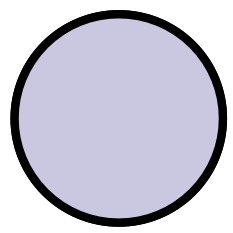
\includegraphics[width=0.015\textwidth, height=0.015\textwidth]{figures/deployment-case-study.png}}

    %Tulsa
	& Jun. 2012 \raisebox{-.2\height}{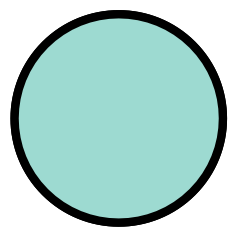
\includegraphics[width=0.015\textwidth, height=0.015\textwidth]{figures/adoption-case-study.png}}

    %Ryan
	& Oct. 2012 \raisebox{-.2\height}{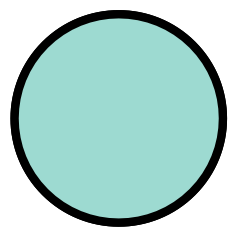
\includegraphics[width=0.015\textwidth, height=0.015\textwidth]{figures/adoption-case-study.png}}

    %Guns
	& Dec. 2012 \raisebox{-.2\height}{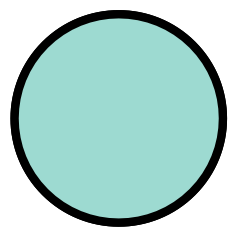
\includegraphics[width=0.015\textwidth, height=0.015\textwidth]{figures/adoption-case-study.png}}

    %Dallas
	& Aug. 2013 \raisebox{-.2\height}{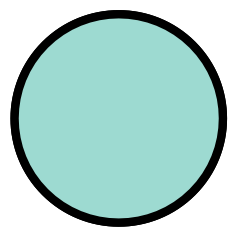
\includegraphics[width=0.015\textwidth, height=0.015\textwidth]{figures/adoption-case-study.png}}

    %NewYork
	& Dec. 2013 \raisebox{-.2\height}{\includegraphics[width=0.015\textwidth, height=0.015\textwidth]{figures/adoption-case-study.png}}

    \\

    \cellcolor{gray!20}
    {\it Version}

	%iraq-sec
	& {\it v2} / desktop

    %Tulsa
	& {\it v2} / desktop

    %Ryan
	& {\it v2} / desktop

    %Guns
	& {\it v3} / web

    %Dallas
	& {\it v4} / web

    %NewYork
	& {\it v4} / web

    \\

    \hline
    \cellcolor{gray!20}
    {\it Document Collection}

    %iraq-sec
    &666 reports / 4,500 pages from \ac{FOIA} (scanned using \ac{OCR}).

    %Tulsa
    &5,996 email messages from \ac{FOIA}.

    %Ryan
    &8,680 pages of correspondence from multiple \ac{FOIA}s (scanned using \ac{OCR}).

    %Guns
    & 2 collections of online discussion board comments (757 in the first, 521 in the second).

    %Dallas
    & 5 collections of email messages from \ac{FOIA}s, ranging from 1,858 to 4,653 messages.

	%NewYork
    & 1,680 proposed and passed bills retrieved with NY Senate Open Legislation \ac{API}.
    
    \\

    \hline
	\cellcolor{gray!20}
    {\it Task}

    %iraq-sec
    & {\bf T1}: {\tt generate\index{{\tt discover}} hypotheses $\rightarrow$ explore\index{{\tt explore}} $\rightarrow$ summarize\index{{\tt summarize}}}

    %Tulsa
    & {\bf T2}: {\tt verify\index{{\tt discover}} hypotheses $\rightarrow$ locate\index{{\tt locate}} $\rightarrow$ identify}\index{{\tt identify}}

    %Ryan
    & {\bf T2}: {\tt verify\index{{\tt discover}} hypotheses $\rightarrow$ locate\index{{\tt locate}} $\rightarrow$ identify}\index{{\tt identify}}

    %Guns
    & {\bf T1}: {\tt generate\index{{\tt discover}} hypotheses $\rightarrow$ explore\index{{\tt explore}} $\rightarrow$ summarize\index{{\tt summarize}}}

    %Dallas
    & {\bf T2}: {\tt verify\index{{\tt discover}} hypotheses $\rightarrow$ locate\index{{\tt locate}} $\rightarrow$ identify}\index{{\tt identify}}

	%NewYork
    & {\bf T2}: {\tt verify\index{{\tt discover}} hypotheses $\rightarrow$ locate\index{{\tt locate}} $\rightarrow$ identify}\index{{\tt identify}}
    
    \\

    \hline
	\cellcolor{gray!20}
    {\it Outcome}

    %iraq-sec
    & Summarized\index{{\tt summarize}} prevalence of document categories.

    %Tulsa
    & Located\index{{\tt locate}} evidence supporting hypothesis.

    %Ryan
    & Located\index{{\tt locate}} a small subset of document clusters relevant to hypothesis.

    %Guns
    & Summarized\index{{\tt summarize}} using exemplar documents. 

    %Dallas
    & Could not locate\index{{\tt locate}} evidence to support hypothesis.

	%New York
    & Proved non-existence of evidence.
    
    \\

    \hline

  \end{tabular}
  \caption
  [
    A summary of the six case studies.
  ]
  {
    A summary of the six case studies; deployment-phase case studies are represented as \raisebox{-.2\height}{\includegraphics[width=0.015\textwidth, height=0.015\textwidth]{figures/deployment-case-study.png}} (purple circles),while adoption-phase case studies are represented as \raisebox{-.2\height}{\includegraphics[width=0.015\textwidth, height=0.015\textwidth]{figures/adoption-case-study.png}} (turquoise circles).
  }
  \label{overview:tab:case-studies}
  \end{center}
\end{table}

%-|-|-|-|-|-|-|-|-|-|-|-|-|-|-|-|-|-|-|-|-|-|-|-|-|-|-|-|-|-|-|-|-|-|-|-|-

%-------------------------------------------------------------------------

\subsection{Think-Aloud Evaluation}
\label{overview:eval-usability}

%-------------------------------------------------------------------------

To complement our case study\index{case study} observations, we also solicited feedback from other journalists\index{journalism}.
After the deployment of the web-based {\it Overview}\index{Overview (document mining tool)} {\it v3}, which included usage tracking, we observed that {\it Overview}\index{Overview (document mining tool)} and its individual features were not being used to the extent that we had hoped.
We suspected usability problems so we embarked on a discount usability testing program inspired by the work of \citet{Nielsen2000}: five na\"{i}ve journalists\index{journalism} were independently presented with an example document collection\index{document data}, such as the collection featured in \autoref{overview:fig:overview-v2}, and asked to narrate their actions as they interacted with {\it Overview}\index{Overview (document mining tool)} using a think-aloud\index{evaluation!think-aloud evaluation} protocol\footnote{Think-aloud protocols are limited in that they do not capture automatic, non-conscious reactions to stimuli. The retrospective introspection of our case study\index{case study} interviews is similarly limited. Interaction logs and screen captures may provide some indication of non-conscious reactions to stimuli. Eye-tracking equipment may provide additional indication of these reactions. However, these think-aloud sessions were performed opportunistically in non-laboratory settings, and we were unable to gather additional data.}, resulting in a qualitative understanding of usability problems.
% RR: p. 86. Think-aloud protocols. Do these really capture what's going on? People's conscious understanding of why they do what they do is iffy at best. (cf. the low rate of adoption described on p. 96.) And what about the use of automatic, non-conscious procedures? Shouldn't we design for them?

All who participated in these think-aloud sessions found {\it Overview}\index{Overview (document mining tool)} to be confusing; much of this confusion was due to the visual complexity of its multiple-view interface, as well as a lack of affordances for common and critical interactions\index{interaction}, such as {\tt selecting}\index{{\tt select}} a document to read. 
We suspect that many previous document set visualization tools would face similar usability problems in real workflows\index{workflows}, either by lacking a robust document {\tt import}\index{{\tt import}} feature, or by not providing a means\index{task!means} to read individual documents~\cite{Cui2011}.
An exception is Jigsaw, whose developers have noted and overcome similar problems \cite{Gorg2014}.
In the next section, we discuss how the design of {\it v4} resolved these usability problems.

%-------------------------------------------------------------------------
%-------------------------------------------------------------------------

\section{Analysis}
\label{overview:analysis}

%-------------------------------------------------------------------------
%-------------------------------------------------------------------------

Given our observations or real world usage, we now revisit our initial task abstraction\index{task!task abstraction} and discuss the rationale for {\it Overview}'s\index{Overview (document mining tool)} design.

%-------------------------------------------------------------------------

\subsection{Task Abstractions Reconsidered}
\label{overview:task-abstraction-reconsidered}

%-------------------------------------------------------------------------

% \js{
% iraq-sec -> summarize by classification
% tulsa -> locate evidence
% gun -> summarize through exemplars
% ryan -> locate subset
% dallas -> locate evidence
% newyork -> prove non-existence
% }

After the {\sc guns} case study\index{case study}, we struggled to distinguish between journalists'\index{journalism} goals, approaches, and outcomes.
Specifically, the {\sc tulsa} and {\sc ryan} journalists\index{journalism} used {\it Overview}\index{Overview (document mining tool)} in more directed and systematic ways that we did not anticipate, in that they sought to {\tt locate}\index{{\tt locate}} specific evidence or a subset of clusters that were relevant to a pre-existing hypothesis, forcing us to reconsider our initial task abstraction\index{task!task abstraction} of {\it ``exploring''}\index{{\tt explore}} a document cluster structure, which was based on the {\sc warlogs} use case.
A number of previous tools aim to help people to {\it ``explore''}\index{{\tt explore}} a document collection\index{document data} (\eg~\cite{Chaney2012,Cui2011,Dou2013,Endert2012b}), though few of these tools have been evaluated\index{evaluation} with people who work in a specific target domain who bring their own data, making us suspect that this imprecise term often masks a lack of understanding of the tasks\index{task} that people perform.

In48 \autoref{ch:typology}, we proposed a typology\index{task!task typology} of abstract visualization tasks\index{task!task abstraction}, the purpose of which was precisely to articulate such differences in the use of visualization tools at multiple levels of abstraction. 
According to this typology\index{task!task typology}, a task\index{task} description is broken down into {\it why}\index{{\tt why}} data is visualized, {\it what}\index{{\tt what}} dependencies a task\index{task} might have, and {\it how}\index{{\tt how}} the task\index{task} is supported.
{\it How}\index{{\tt how}} is somewhat orthogonal to {\it why}\index{{\tt why}}, as exemplified by the differences in usage reported in the previous section.
We applied this typology\index{task!task typology} to the coding\index{coding (qualitative data analysis)} of our observational data, characterizing two different tasks\index{task}, {\bf T1} and {\bf T2}, that replace and improve upon our initial task abstraction\index{task!task abstraction}. 
In this section, we will use the vocabulary and notation of this typology\index{task!task typology} to focus on {\it why}\index{{\tt why}} and {\it what}\index{{\tt what}}; in \autoref{overview:rationale}, we analyze {\it how}\index{{\tt how}} {\it Overview}\index{Overview (document mining tool)} supports these tasks\index{task}.

\bstart{T1: {\tt generate hypotheses} $\rightarrow$ {\tt explore} $\rightarrow$ {\tt summarize}}
When approaching a collection of leaked documents or a corpus of social media content, a journalist\index{journalism} may have little prior knowledge regarding the collection's content, eliciting a need to {\tt generate hypotheses}\index{{\tt discover}} and to ask {\it ``what's in this collection?''}.
To support the generation of hypotheses, a journalist\index{journalism} must be able to {\tt explore}\index{{\tt explore}} a document collection\index{document data} and {\tt summarize}\index{{\tt summarize}} clusters of documents.
The term {\tt explore}\index{{\tt explore}} is defined more precisely in our typology\index{task!task typology} as a form of {\tt search}\index{{\tt search}} in which neither the identity nor the location of a search target are known a priori.
In the context of a document collection\index{document data}, a search target may be content within a document, an individual document itself, a cluster of related documents, or an arbitrary set of documents and clusters.
{\tt Exploring}\index{{\tt explore}} is distinguished from {\tt browsing}\index{{\tt browse}}, in which the location of a search target is known but its identity is not, {\tt locating}\index{{\tt locate}}, in which the converse is true, and {\tt lookup}\index{{\tt lookup}}, in which both the location of the target and its identity are known. 
The result of {\tt summarizing}\index{{\tt summarize}} is a compressed representation of the full contents of the document collection\index{document data}, such as the categories and counts produced in the {\sc iraq-sec} case study\index{case study}, or the exemplar documents that the journalist\index{journalism} ultimately {\tt selected}\index{{\tt select}} in {\sc guns} case study\index{case study}.

\bstart{T2: {\tt verify hypotheses} $\rightarrow$ {\tt locate} $\rightarrow$ {\tt identify}}
In contrast, a journalist\index{journalism} who asks for documents via \ac{FOIA} request typically has some pre-existing hypotheses, and their aim is to {\tt verify}\index{{\tt discover}}, {\tt refute}, or {\tt refine} these hypotheses by {\tt locating}\index{{\tt locate}} evidence.
In these cases, a journalist\index{journalism} likely has a sense of what the documents are about, but they may not be able to specify the evidence they seek in terms of a standard keyword search (for example, ``corruption'' would not suffice), and there may also be unexpected but valuable material waiting to be discovered.
In the language of our typology\index{task!task typology}, the aim is to {\tt locate}\index{{\tt locate}} and {\tt identify}\index{{\tt identify}} clusters containing potential evidence, beginning with those labelled by interesting keyword terms; alternatively, a journalist\index{journalism} will {\tt locate}\index{{\tt locate}} documents containing specific search terms and subsequently {\tt browse}\index{{\tt browse}} and {\tt identify}\index{{\tt identify}} related documents found in the same cluster.
{\bf T2} describes the use of {\it Overview}\index{Overview (document mining tool)} in the {\sc tulsa}, {\sc ryan}, {\sc dallas}, and {\sc ny} case studies\index{case study}.

Throughout both {\bf T1} and {\bf T2}, a journalist\index{journalism} will often {\tt produce}\index{{\tt produce}} notes or annotations\index{{\tt annotate}} for documents as they {\tt generate}\index{{\tt discover}}, {\tt verify}\index{{\tt discover}}, or {\tt refine} their hypotheses, perhaps {\tt comparing}\index{{\tt compare}} documents to each other or to secondary sources outside of the collection.
{\bf T1} and {\bf T2}, along with the subsequent annotation task, are illustrated using the visual notation of our typology\index{task!task typology} in \autoref{fig:overview:tasks} and \autoref{fig:overview:tasks:annotate}, respectively, in the addendum (\autoref{overview:addendum}) at the end of this chapter.

%-------------------------------------------------------------------------

\subsection{Design Rationale}
\label{overview:rationale}

%-------------------------------------------------------------------------

With a more precise understanding of journalists'\index{journalism} tasks\index{task}, we now analyze the rationale for our visual encoding\index{visual encoding} and interaction\index{interaction} design choices in the hope that our choices may transfer to other domain problems involving similar data\index{data abstraction} and task abstractions\index{task!task abstraction}.

\bqstart{Why show a tree?}
{\it Trees\index{visual encoding!tree} afford structured and systematic exploration\index{{\tt explore}}.}
When a document collection\index{document data} contains separable clusters of similar documents, a tree-based visual encoding\index{visual encoding!tree} affords a systematic and, if desired, exhaustive traversal of these clusters. 
The {\sc tulsa} case study\index{case study} is an example where the journalist\index{journalism} based his choice of which documents to read based on the structure of the tree\index{visual encoding!tree}, sweeping from left to right.
The {\it Topic Tree}\index{visual encoding!tree} also includes a visual encoding\index{visual encoding} of applied tags, which makes it possible for a person to {\tt identify}\index{{\tt identify}} the documents they have and have not already tagged, and how tags correspond to clusters.

\bqstart{How to show a tree?}
{\it Emphasize interior nodes (not edges or leaves); instill trust\index{trust} in the underlying algorithm.}
The {\it Topic Tree}\index{visual encoding!tree} in the first two versions of {\it Overview}\index{Overview (document mining tool)} (\autoref{overview:fig:overview-v2}) rendered all clusters as identical nodes.
While tree-based visual encodings\index{visual encoding!tree} are often associated with the task\index{task} of path tracing and determining connectivity~\cite{Lee2006}, people who use {\it Overview}\index{Overview (document mining tool)} are primarily interested in the properties of nodes corresponding to document clusters, such as the number of documents contained by a cluster, or the key terms that describe these documents.

The {\it Topic Tree}\index{visual encoding!tree} of {\it v3-4} directly {\tt encodes}\index{{\tt encode}} cluster size as node width; this design choice allows a person to {\tt compare}\index{{\tt compare}} cluster sizes directly, or work systematically from larger to smaller topics, of particular use when trying to {\tt summarize}\index{{\tt summarize}} a document collection\index{document data} to some desired degree of detail ({\bf T1}).
In enlarging the width of nodes, it also became possible to {\tt encode}\index{{\tt encode}} the number of documents tagged within the cluster as a colour label having a width proportional to the size of the node, as shown in \autoref{overview:fig:overview-v4}.
We opted not to use a space-filling treemap\index{visual encoding!treemap} visual encoding\index{visual encoding} of hierarchical document clusters\index{document data} because this approach would place too much emphasis on leaf nodes; when {\tt summarizing}\index{{\tt summarize}} a collection ({\bf T1}) or when {\tt locating}\index{{\tt locate}} a subset of documents ({\bf T2}), the mid-level interior nodes in the tree\index{visual encoding!tree} are typically the most informative.
While less space efficient, a tree\index{visual encoding!tree} with variable-width nodes provides more flexibility, especially given the differences between {\bf T1} and {\bf T2}.

With larger nodes, we were able to display cluster keyword terms directly in the node itself, rather than in a separate {\it Cluster List} view, as in {\it v1-2}, which displayed keywords only for the selected\index{{\tt select}} cluster and its descendants.
Displaying keywords within nodes allows a person to {\tt compare}\index{{\tt compare}} keywords at a glance, both between and within clusters.

The design of the {\it Topic Tree}\index{visual encoding!tree} required a balance between usability and cluster fidelity: in {\it v3}, there was no limit on the number of children allowed for each node, a situation reported to be overwhelming by journalists\index{journalism} who participated in the think-aloud evaluation\index{evaluation!think-aloud evaluation}.
When a node can have many children, tree\index{visual encoding!tree} exploration\index{{\tt explore}} reduces to linear search; for this reason, the maximum number of child nodes was limited in {\it v4} by switching to a recursive adaptive {\it K}-means algorithm~\cite{Pham2005}\index{algorithms!clustering} with an upper limit of five children per node.

We added explicit cluster fidelity labels to the {\it Topic Tree}\index{visual encoding!tree} nodes in {\it v4}
to help people interpret the content of a cluster: the labels {\it ``Some''}, {\it ``Most''}, and {\it ``All''} show how many documents in a cluster contain each keyword and thus signal the consistency of topics found in that node, as shown in \autoref{overview:fig:overview-v4}.
These labels help a person to decide whether to treat the node as a conceptual unit that might be tagged as a whole, or expand it to examine its children individually.
They help a person assess cluster consistency and separability and serve to build trust\index{trust} in the clustering algorithm~\cite{Chuang2012}\index{algorithms!clustering}.
Previously, people had to judge the topical consistency of a cluster by examining the individual documents within it, or by referring to the scatterplot\index{visual encoding!scatterplot} in a way that \citet{Sedlmair2013} demonstrated to be difficult for dimensionally reduced\index{dimensionality reduction (DR)} data.

\begin{sloppypar}
\bqstart{How to interact with a tree?}
{\it Selective pruning and informative tooltips.}
In {\it v1-v2}, people were able to clarify the {\it Topic Tree}\index{visual encoding!tree} by pruning ({\tt aggregating}\index{{\tt aggregate}}) small nodes, according to a threshold {\tt selected}\index{{\tt select}} from a set of seven coloured radio buttons below the {\it Topic Tree}\index{visual encoding!tree}.
Our case studies\index{case study} revealed that many people never understood that the variable tree-pruning threshold used in {\it v1-v2} was hiding nodes from them, a problem especially for those intent on {\tt locating}\index{{\tt locate}} evidence or proving the non-existence of evidence ({\bf T2}).
We replaced threshold-based node pruning with a selective expand/collapse option on each node; when combined with panning and zooming, these interactions\index{interaction} provide people with a fine-grained control over focus and context.
\end{sloppypar}

Upon {\tt selecting}\index{{\tt select}} a node in {\it v1-v2}, keywords for the selected\index{{\tt select}} cluster and its descendants were shown in a status bar between the {\it Topic Tree}\index{visual encoding!tree} and the {\it Cluster List}, however these were spatially removed from a person's point of focus.
To resolve this, we added tooltips in {\it v3} that show cluster keywords when the cursor hovers over a node.

\bqstart{Why no scatterplot?}
{\it Unstructured exploration\index{{\tt explore}} is redundant for} {\bf T1} {\it and} {\bf T2}.
Using scatterplots\index{visual encoding!scatterplot} to visualize document collections\index{document data} is an approach common to previous work~\cite{Chen2009,Granitzer2004,Endert2012b,Leaksplorer,Paulovich2007}.
We thought that a scatterplot\index{visual encoding!scatterplot} would allow people to judge cluster size, quality, and separability~\cite{Sedlmair2013}.
However, scatterplots\index{visual encoding!scatterplot} do not directly show cluster content, such as document keywords, unless tooltips or point aggregation is used.
We did not pursue the use of these design choices because we discovered that the scatterplot\index{visual encoding!scatterplot} was seldom used in the case studies\index{case study} of journalists\index{journalism} who adopted\index{adoption} {\it Overview}\index{Overview (document mining tool)}.
The {\sc tulsa} journalist\index{journalism} was an exception in that he used the scatterplot\index{visual encoding!scatterplot} to {\tt locate}\index{{\tt locate}} untagged documents containing potential evidence after extensive use of the {\it Topic Tree}\index{visual encoding!tree} ({\bf T2}).
This task\index{task} would have been better served by providing a direct way to show how many untagged documents a node contains; the {\it ``Show Untagged''} button introduced in {\it v4} accomplishes this.

Ultimately, we realized that a scatterplot\index{visual encoding!scatterplot} does not help people overcome the burden of choice overabundance when determining which cluster to investigate next~\cite{Schwartz2003}, whereas the tree-based hierarchical clustering\index{algorithms!clustering} used in the {\it Topic Tree}\index{visual encoding!tree} affords a form of structured {\tt navigation}\index{{\tt navigate}}.
In addition, the cluster fidelity labels introduced in {\it v4} help people to assess cluster consistency and separability, thereby eliminating any further need for a scatterplot\index{visual encoding!scatterplot}.  

\bqstart{Why tags?}
{\it Tags provide simple annotation\index{{\tt annotate}}, progress tracking, and human-defined semantics.}
Tagging was used extensively in five of the six case studies\index{case study}. 
Some tags aligned with cluster boundaries ({\sc iraq-sec}, {\sc ryan}, and the first set of tags created in {\sc tulsa}), while other tags appeared throughout the tree\index{visual encoding!tree} ({\sc dallas}, {\sc ny}, and the second set of tags created in {\sc tulsa}).
Tags are a simple and flexible form of {\tt annotation}\index{{\tt annotate}} that help people track where they have been and what they have learned. 
They can also be used to impose a context-specific organization scheme on a document collection\index{document data}.
No single clustering will meet all analysis needs, since any high-dimensional dataset\index{high-dimensional data} is likely to have multiple cross-cutting semantically interesting clusterings~\cite{Grimmer2011}. 
The ``best'' clustering will depend on the documents and the story.
{\it Overview}\index{Overview (document mining tool)} does not support manual re-arrangement\index{{\tt arrange}} of the {\it TopicTree} hierarchy, as in tools such as HierarchicalTopics~\cite{Dou2013}.
Instead, we support manual tagging as a simple and flexible way for people to impose their own semantics on a document collection\index{document data}, where the cluster structure can be leveraged as a useful scaffold when it matches a person's mental model, but ignored when it does not.
The most recent feature added to {\it Overview}\index{Overview (document mining tool)}, developed after the case studies\index{case study} in this chapter, supports the creation of multiple trees\index{visual encoding!tree}, giving different views of same document collection\index{document data}. 
A person can control the clustering by entering words to ignore, which prevents {\it Overview}\index{Overview (document mining tool)} from clustering based on document letterhead or boilerplate text, and by entering especially important words which are weighted higher when constructing document vectors. 
It is also possible to create a tree\index{visual encoding!tree} containing only a subset of the documents, specified by {\tt selecting}\index{{\tt select}} an existing tag.

\bqstart{Multiple views: how many and how to coordinate?}
{\it Less is more; provide obvious affordances.}
The evolving design of {\it Overview}\index{Overview (document mining tool)} recalls the challenges and considerations for designing multiple view tools, which we have discussed elsewhere~\cite{Lam2010}.
These considerations include determining the appropriate number of discrete views, the arrangement\index{{\tt arrange}} of these views, and how these views should be coordinated\index{view coordination}.
A consensus on these questions has not yet been reached, as multiple-view visualization tools range from dual-view to over twenty, with a similar range in view coordination patterns~\cite{Weaver2007}.

The {\sc caracas} pilot case study\index{case study} with {\it Overview v1} revealed that the {\it Document Viewer} was too small and the {\tt selection}\index{{\tt select}} of documents and clusters across the different views was poorly coordinated\index{view coordination}\index{view coordination}.
Despite improvements to view coordination in {\it v2} and {\it v3}, the views were not always well understood; for example, those who participated in the think-aloud evaluation\index{evaluation!think-aloud evaluation} did not initially realize that the {\it Document List}, displayed as a line of keywords for each document, was in fact a list of {\tt selectable}\index{{\tt select}} documents.
In {\it v4}, {\it Overview}'s\index{Overview (document mining tool)} interface was streamlined into three views coordinated\index{view coordination} with linked {\tt selection}\index{{\tt select}} and highlighting: the {\it Topic Tree}\index{visual encoding!tree}, a consolidated {\it Document Viewer/List} featuring document titles and list {\tt navigation}\index{{\tt navigate}} controls, and a list of {\it Tags}; as described above, we removed the scatterplot\index{visual encoding!scatterplot} and {\it Cluster List}, both made redundant by the redesigned {\it Topic Tree}\index{visual encoding!tree}.
While we might have made {\it Overview}\index{Overview (document mining tool)} a single-view tool, we instead reasoned that having the {\it Topic Tree}\index{visual encoding!tree} visible provides helpful context when reading a document and deciding what to read next.

\bqstart{How to support workflows?}
{\it Simplify for infrequent use; reduce data wrangling.}
Our findings show that simplicity and learnability are critical for journalists\index{journalism}, because any one journalist\index{journalism} only deals with large document collections\index{document data} intermittently.

After {\it Overview v2} was deployed and promoted within the journalism\index{journalism} community, it became clear that many people had great difficulty downloading, installing, and configuring it.
Additionally, {\it v2} could only {\tt import}\index{{\tt import}} documents in a \ac{CSV} file; we quickly learned that journalists\index{journalism} receive document collections\index{document data} in every conceivable format, from stacks of paper to database dumps.
We confirmed that the need to wrangle data into compatible formats is a considerable barrier to adopting\index{adoption} a visualization tool into an analysis workflow\index{workflows}, as discussed in a recent research agenda~\cite{Kandel2011}.
We should not expect journalists\index{journalism} to write custom data wrangling scripts, as the {\sc ny} journalist\index{journalism} had to do.
To minimize the amount of configuration and wrangling required, the web-based {\it Overview v3-v4} required no installation and supported {\tt import}\index{{\tt import}} from a folder of \ac{PDF} documents or from DocumentCloud\footnote{\url{http://documentcloud.org/}}, a document hosting service used by journalists\index{journalism} which can itself ingest a wide variety of formats.
Without this integration, we suspect that the {\sc dallas} journalist\index{journalism} would have been unable to make use of {\it Overview}\index{Overview (document mining tool)}.
The DocumentCloud interface is integrated into {\it Overview}'s\index{Overview (document mining tool)} {\it Document Viewer}, which includes a function for {\tt annotating}\index{{\tt annotate}} documents with notes. 

We also added full-text keyword search in {\it v4}, as members of the journalism\index{journalism} community and our case study\index{case study} journalists\index{journalism} had expressed a desire to flexibly alternate between {\tt locating}\index{{\tt locate}} clusters in the {\it Topic Tree}\index{visual encoding!tree} and a directed search for {\tt locating}\index{{\tt locate}} documents of interest, without having to use a search tool such as grep or DocumentCloud's search interface. 
We expect that the {\sc tulsa} and {\sc ryan} journalists\index{journalism}, both performing {\bf T2} with {\it v2}, would have benefited from this keyword search feature, and that the absence of this feature would have been a deterrent for the {\sc dallas} and {\sc ny} journalists\index{journalism}, who also performed {\bf T2}.

We note that the use of {\it Overview}\index{Overview (document mining tool)} forms part of a larger investigation and reporting workflow\index{workflows}: each case study\index{case study} journalist\index{journalism} combined its use with many computer-assisted and non-computer-assisted methods for data collection, data transformation, and eventual story presentation\index{storytelling}.

\bstart{Summary}
This section presented seven lessons or guidelines that can be applied to the design of visualization tools for document data\index{document data} in particular, though we expect that these lessons may also be transferable to tools that address other forms of hierarchically-structured data\index{hierarchical data}:

\begin{itemize}
    \item Why show a tree?\index{visual encoding!tree} {\it Trees afford structured and systematic exploration\index{{\tt explore}}.}
    \item How to show a tree?\index{visual encoding!tree} {\it Emphasize interior nodes (not edges or leaves); instill trust\index{trust} in the underlying algorithm.}
    \begin{sloppypar}
    \item How to interact with a tree?\index{visual encoding!tree} {\it Selective pruning and informative tooltips.}
    \end{sloppypar}
    \item Why no scatterplot?\index{visual encoding!scatterplot} {\it Unstructured exploration\index{{\tt explore}} is redundant.}
    \item Why tags? {\it Tags provide simple annotation\index{{\tt annotate}}, progress tracking, and human-defined semantics.}
    \item Multiple views: how many and how to coordinate? {\it Less is more; provide obvious affordances.}
    \item How to support workflows?\index{workflows} {\it Simplify for infrequent use; reduce data wrangling.}
\end{itemize}

%-------------------------------------------------------------------------
%-------------------------------------------------------------------------

\section{Discussion}
\label{overview:discussion}

%-------------------------------------------------------------------------
%-------------------------------------------------------------------------

In this section, we discuss the value and logistics of conducting field studies involving multiple deployments and the analysis of adoption\index{adoption}, as well as the limitations of this type of research.

\bqstart{Why study adoption?}
As with any iterative human-centred design process, it is difficult to know when to declare success; we consider adoption\index{adoption} defined as repeated instances of self-initiated use to be a form of success. 
Adoption\index{adoption} is particularly interesting in the domain of journalism\index{journalism} because tool use is a decision made separately by each journalist\index{journalism} for each story, rather than dictated by a central authority.

Though the visualization design process is cyclical and may include multiple deployments, there are surprisingly few papers that comment on the adoption\index{adoption} of a visualization tool without the prompting of designers: in a recent survey of eight hundred visualization papers containing an evaluation\index{evaluation} component, only five commented on adoption~\cite{Lam2012}\index{adoption}. 
Of these, two provide a thorough description of who adopted\index{adoption} their visualization tool, how it had been used, whether it was still in use, and what problems people reported~\cite{Kincaid2005,McKeon2009}.
Our work adds to this short list, as does the recent study of Jigsaw's adoption~\cite{Kang2012}\index{adoption}.

Many visualization design studies\index{design studies} report on deployment to a target group of individuals and evaluate\index{evaluation} their reaction to the tools during a period of intense study, but our own experience and personal communication with other practitioners leads us to believe that visualization tool use typically drops off after a paper is submitted. 
\citet{Gonzalez2003a} provide a rare example of explicitly checking back after this time period; they found that their target population did not adopt\index{adoption} the visualization tool despite the promising initial results reported in their original paper, and conjecture that a misunderstanding of workflow\index{workflows} was the primary factor behind this lack of adoption\index{adoption}. 
We conjecture that this situation might be the common case, and that longer-term adoption\index{adoption} rates may be very low for research prototypes. 
Sustained follow-up by researchers until adoption\index{adoption} is achieved provides a way to disambiguate whether the barrier to adoption\index{adoption} is truly only a workflow\index{workflows} issue, or an indication that the tool failed to address the true needs of the people for whom the tool was built.

\bstart{The logistics of studying adoption}
Before {\it Overview}\index{Overview (document mining tool)} was deployed, we could not have fully predicted {\it why}\index{{\tt why}} and {\it how}\index{{\tt how}} journalists\index{journalism} would approach large document collections\index{document data}; we were unable to verify the correctness of our task\index{task!task abstraction} and data abstractions\index{data abstraction}.
{\it Overview}\index{Overview (document mining tool)} is sufficiently novel that its value could not be assessed without adequately functional prototypes.
We argue that this situation is common in visualization because of the complexity of the data and tasks\index{task} at play, recalling the argument of \citet{Lloyd2011} about the need for {\it data sketches}\index{data sketch}: functional example designs for establishing context of use and eliciting requirements\footnote{Unlike typical \ac{HCI} approaches such as paper prototyping, functional example designs in a visualization context entails the development of interactive software prototypes.}.
They contrasted their design-first approach, illustrated by the red trajectories in \autoref{overview:fig:hcd-loops}, to a design-then-evaluate\index{evaluation} approach (the green trajectory) and to an approach grounded in a person's context~\cite{Isenberg2008} (the blue trajectory).
The purple trajectory illustrates that close collaboration with domain experts from the very start of a project means they bring expertise about requirements to the table, so it is not a design-first endeavour. 
The multiple loops in the purple trajectory emphasize the importance of deploying a visualization tool as a precursor to evaluation\index{evaluation}, and we note that after these loops the trajectory ends at context of use: it took several deployments and case studies\index{case study} of self-initiated journalists\index{journalism} who adopted\index{adoption} {\it Overview}\index{Overview (document mining tool)} before we attained a clear understanding of journalists'\index{journalism} tasks\index{task} and their broader analysis workflows\index{workflows}.

%-|-|-|-|-|-|-|-|-|-|-|-|-|-|-|-|-|-|-|-|-|-|-|-|-|-|-|-|-|-|-|-|-|-|-|-|-

 \begin{figure}
	\centering
	\includegraphics[width=\textwidth]{figures/hcd-loops}
	\caption
	[
	    The human-centred design process development cycle.
	]
	{
	    The human-centred design process development cycle, in which \citet{Lloyd2011} discern between alternative entry points (A,B) and between design-then-evaluate (green), grounded (blue), and their own approach in which example designs are used to establish context of use and elicit requirements (red). In contrast, we begin with some requirements at point C, and only after multiple deployments do we arrive at a clear understanding of context of use (purple). Figure adapted and extended from \citet{Lloyd2011}.
	}
	\centering
	\label{overview:fig:hcd-loops}
\end{figure}

%-|-|-|-|-|-|-|-|-|-|-|-|-|-|-|-|-|-|-|-|-|-|-|-|-|-|-|-|-|-|-|-|-|-|-|-|-

Our use of case studies\index{case study} to study adoption\index{adoption} is methodologically similar to qualitative longitudinal evaluation\index{evaluation} studies described in previous work~\cite{Lloyd2011,Saraiya2006,Shneiderman2006}.
Our approach differs from these in that we engaged a different set of people at each stage of design, rather than the same set of people.
This difference reflects {\it Overview}'s\index{Overview (document mining tool)} context of use: repeat usage cannot be predicted and {\it Overview}\index{Overview (document mining tool)} is only appropriate for some investigations; we have yet to encounter a journalist\index{journalism} who specializes in investigations pertaining to large document collections\index{document data}.

%-------------------------------------------------------------------------
%-------------------------------------------------------------------------

\section{Summary}
\label{overview:conclusion}

We presented a field study of {\it Overview}\index{Overview (document mining tool)}, an application for the systematic analysis of large document collections\index{document data}.
{\it Overview}\index{Overview (document mining tool)} has proven to be useful, having been used in investigations leading to at least nine published stories.
Using the typology\index{task!task typology} of visualization tasks proposed in \autoref{ch:typology}, we characterized two task abstractions\index{task!task abstraction} based on findings from six case studies\index{case study}.
Given our data and task abstractions\index{task!task abstraction}, we rigorously analyzed the effectiveness of {\it Overview}'s\index{Overview (document mining tool)} visual encoding\index{visual encoding} and interaction\index{interaction} design.
Our analysis may transfer beyond the domain of journalism\index{journalism}, and speaks to the design and evaluation\index{evaluation} of other visualization tools for supporting the analysis of document collections\index{document data} and clustered dimensionally reduced\index{dimensionality reduction (DR)} data.
Finally, this work adds to the small number of studies found in the visualization literature that include observations of adoption\footnote{While studies of adoption and appropriation may be common in the \ac{HCI} community, they are rare in the visualization literature.}\index{adoption}; in observing real world usage by self-initiated journalists\index{journalism}, we presented detailed evidence to support the contention that that several iterations of design and deployment are required before fully understanding {\it why}\index{{\tt why}} and {\it how}\index{{\tt how}} a visualization tool will be used in practice.

%-------------------------------------------------------------------------
%-------------------------------------------------------------------------

\section{Addendum}
\label{overview:addendum}

\autoref{fig:overview:tasks}\footnote{\autoref{fig:overview:tasks} and \autoref{fig:overview:tasks:annotate} did not appear in our paper about {\it Overview}~\cite{Brehmer2014}.} illustrates the two tasks\index{task} that we characterized in \autoref{overview:task-abstraction-reconsidered}; colours correspond to the {\it why-what-how} structure of our task typology\index{task!task typology} (see \autoref{typology:fig:typology})\footnote{We use the revised typology described in \autoref{drvistasks:typology}.}.
\autoref{fig:overview:tasks} indicates the {\it how}\index{{\tt how}} and {\it what}\index{{\tt what}} aspects of these two tasks\index{task} explicitly, as this information was discussed implicitly throughout this chapter. 
In {\bf T1}, the {\tt input}\index{{\tt input}} is a document collection\index{document data} and the {\tt output}\index{{\tt output}} is evidence to either refute or verify\index{{\tt discover}} a hypothesis.
In {\bf T2}, the {\tt input}\index{{\tt input}} is once again a document collection\index{document data}, however the {\tt output}\index{{\tt output}} is a set of exemplar documents or a set of clusters that can be used to {\tt summarize}\index{{\tt summarize}} the entire collection.
{\it Overview}\index{Overview (document mining tool)} supports both of these tasks\index{task} via {\tt encoding}\index{{\tt encode}} the document collection\index{document data} as a tree\index{visual encoding!tree}, by allowing people to interactively {\tt navigate}\index{{\tt navigate}} this tree structure\index{visual encoding!tree}, to {\tt select}\index{{\tt select}} clusters and individual documents, to {\tt aggregate}\index{{\tt aggregate}} (or disaggregate) clusters of documents using the interactive expand and collapse controls on each node of the tree\index{visual encoding!tree}.

\autoref{fig:overview:tasks:annotate} depicts a task\index{task} that follows either {\bf T1} or {\bf T2}, in which the person who uses {\it Overview}\index{Overview (document mining tool)} will {\tt annotate}\index{{\tt annotate}} clusters or individual documents with meaningful tags (a {\tt produce}\index{{\tt produce}} action)\footnote{As per the discussion in \autoref{drvistasks:typology}, we now view {\tt annotate} as a form of {\tt produce}, as indicated in \autoref{fig:overview:tasks:annotate}.}.
To {\tt annotate}\index{{\tt annotate}} documents or clusters with tags, a person {\tt selects}\index{{\tt select}} documents or clusters, {\tt selects}\index{{\tt select}} a tag, and the tag is {\tt encoded}\index{{\tt encode}} as a coloured label for the document or cluster.

%-|-|-|-|-|-|-|-|-|-|-|-|-|-|-|-|-|-|-|-|-|-|-|-|-|-|-|-|-|-|-|-|-|-|-|-|-

 \begin{figure}
	\centering
	\includegraphics[width=\textwidth]{figures/overview-tasks}
	\caption
	[
	   The two tasks characterized in \autoref{overview:task-abstraction-reconsidered}.
	]
	{
	   The two tasks characterized in \autoref{overview:task-abstraction-reconsidered}; colours correspond to the {\it why-what-how} structure of our task typology (see \autoref{typology:fig:typology}), where yellow is {\it why}, green is {\it how}, and grey is {\it what} defined in terms of {\tt inputs} and {\tt outputs}.
	}
	\centering
	\label{fig:overview:tasks}
\end{figure}

%-|-|-|-|-|-|-|-|-|-|-|-|-|-|-|-|-|-|-|-|-|-|-|-|-|-|-|-|-|-|-|-|-|-|-|-|-

%-|-|-|-|-|-|-|-|-|-|-|-|-|-|-|-|-|-|-|-|-|-|-|-|-|-|-|-|-|-|-|-|-|-|-|-|-

 \begin{figure}
	\centering
	\includegraphics[width=\textwidth]{figures/overview-tasks-2}
	\caption
	[
	    The task of {\tt annotating} documents and clusters.
	]
	{
	   The task of {\tt annotating} documents and clusters (which follows {\bf T1} or {\bf T2}); colour conventions follow that of \autoref{fig:overview:tasks}.
	}
	\centering
	\label{fig:overview:tasks:annotate}
\end{figure}

%-|-|-|-|-|-|-|-|-|-|-|-|-|-|-|-|-|-|-|-|-|-|-|-|-|-|-|-|-|-|-|-|-|-|-|-|-

\endinput

%-------------------------------------------------------------------------
%-------------------------------------------------------------------------
%-------------------------------------------------------------------------

\chapter[Design Study\texorpdfstring{:\\ Matches, Mismatches, and Methods: Multiple-View Workflows for Energy Portfolio Analysis}{}]{Design Study\texorpdfstring{:\\ \large{Matches, Mismatches, and Methods: Multiple-View Workflows for Energy Portfolio Analysis}}{}}
\label{ch:emu}

%-------------------------------------------------------------------------
%-------------------------------------------------------------------------
%-------------------------------------------------------------------------

% \begin{epigraph}
%     \item (quote needed)
% \end{epigraph}

\footnote{This chapter is a slightly modified version of our paper {\it Matches, Mismatches, and Methods: Multiple-View Workflows for Energy Portfolio Analysis} by Matthew Brehmer, Jocelyn Ng, Kevin Tate, and Tamara Munzner; in IEEE Transactions on Visualization and Computer Graphics (Proceedings of InfoVis 2015), 22(1), p. 449--458~\cite{Brehmer2015}. \url{http://dx.doi.org/10.1109/TVCG.2015.2466971}. \autoref{emu:addendum} is a new addendum section that is unique to this dissertation.}The energy performance of large building portfolios is challenging to analyze and monitor, as current analysis tools are not scalable or they present derived and aggregated data at too coarse of a level. 
We conducted a visualization design study\index{design studies}, beginning with a thorough work domain analysis\index{work domain analysis} and a classification of data\index{data abstraction} and task abstractions\index{task!task abstraction}. 
We describe visual encoding\index{visual encoding} design choices for time-oriented data\index{time-oriented data} framed in terms of {\it matches} and {\it mismatches}, as well as considerations for workflow design\index{workflows!workflow design}. 
Our designs address several research questions pertaining to scalability, view coordination\index{view coordination}, and the inappropriateness of line graphs\index{visual encoding!line graph} for derived\index{{\tt derive}} and aggregated\index{{\tt aggregate}} data. 
We also present guidelines relating to {\it familiarity}\index{familiarity} and {\it trust}, as well as methodological considerations for visualization design studies\index{design studies}. 
Our designs were adopted\index{adoption} by our collaborators and incorporated into the design of an energy analysis software application that will be deployed to their large client base.

%-------------------------------------------------------------------------
%-------------------------------------------------------------------------

\section{Motivation}
\label{emu:introduction}

%-------------------------------------------------------------------------
%-------------------------------------------------------------------------

Consider a university campus containing about a hundred buildings. 
For a university operations worker looking for opportunities to conserve energy, visualization can be helpful when analyzing and monitoring the energy performance of this large portfolio of buildings. 

In this design study\index{design studies}, we collaborated with a team of people at EnerNOC, a company that develops energy analysis and reporting software for organizations such as commercial business chains, universities, and utility companies.
Our collaborators' goal was to deploy a redesigned version of Energy Manager\index{Energy Manager}, their energy analysis software tool; in doing so, they hoped to retain their existing client base encompassing thousands of organizations, attract new clients, and increase engagement with their software. 
Meanwhile, our goal as researchers was to successfully integrate our research process into our collaborators' software development practice.
We designed and evaluated\index{evaluation} potential visual encodings\index{visual encoding} and interactions\index{interaction} with a variety of stakeholders in an industry setting, which included our collaborators' colleagues as well as their clients.
This chapter documents a success story, where our collaborators committed software development resources and adopted\index{adoption} our designs that resulted from our research.

Visualization researchers and practitioners working in domains unrelated to energy analysis will find several transferable aspects of this chapter, beginning with our classification of data\index{data abstraction} and task abstractions\index{task!task abstraction}.
This project required that we design and promote sophisticated visual analysis by individuals accustomed to unsophisticated visual encoding design choices.
We needed scalable visual encoding\index{visual encoding} and interaction\index{interaction} design choices that can accommodate dozens to hundreds of concurrent time series\index{time-oriented data}.
To complicate matters further, we could not rely upon the visual encoding design choice of a line graph\index{visual encoding!line graph} due to a combination of data semantics and domain convention\index{domain convention}.
Once we found appropriate mappings between visual encoding design choice and individual tasks\index{task}, we next addressed the question of accommodating task sequences\index{task!task sequence}: determining which visual encodings\index{visual encoding} ought to be juxtaposed\index{view coordination!view juxtaposition} in the same display as multiple views on the data\index{view coordination}, and which ought to be presented sequentially.
Coordinating these views also posed a challenge; specifically, we sought to reduce the amount of manual navigation\index{{\tt navigate}} between views\index{view coordination!view sequencing}, as this was an issue with the previous version of Energy Manager\index{Energy Manager}.

The primary contribution of this chapter is a set of design choices and guidelines framed in terms of {\it matches} and {\it mismatches} between abstractions\index{task!task abstraction}\index{data abstraction} and visual encoding\index{visual encoding} design choice for time-oriented data\index{time-oriented data}, guidelines that transfer beyond the energy management\index{energy management} domain.
We also present guidelines relating to the themes of {\it familiarity}\index{familiarity} and {\it trust}.
The former refers to the spectrum between ubiquitous visual encodings\index{visual encoding} and those that a person may have never seen before, while the latter refers to the appropriate display of derived\index{{\tt derive}} and aggregated data, as well as giving people control over these data transformations.
Finally, we contribute methodological advice for visualization design projects.
This includes considerations for designing workflows\index{workflows} that incorporate multiple views\index{view coordination};
while prototyping the visual encoding\index{visual encoding} design of a single view has received considerable attention in the literature~\cite{Lloyd2011}, workflow\index{workflows} prototyping has received far less. 

% We begin by describing our research and design methodology in \autoref{emu:methodology}.
% \autoref{emu:abstractions}, \autoref{emu:existing-tool}, and \autoref{emu:related-work} provide the context around our designs in terms of task and data abstractions, the previous Energy Manager tool, and related work. 
% Our designs are documented throughout \autoref{emu:sandbox}, \autoref{emu:design:visenc}, and \autoref{emu:design:workflows}. 
% We report on which of our designs were adopted by inclusion into our collaborators' product development cycle in \autoref{emu:results}.
% Finally, we reflect on familiarity, trust, and on methodological considerations for visualization design studies in \autoref{emu:discussion}.

%-------------------------------------------------------------------------
%-------------------------------------------------------------------------

\section{Methodology}
\label{emu:methodology}

%-------------------------------------------------------------------------
%-------------------------------------------------------------------------

In this section, we focus on how we conducted our research; we reflect upon our methodological decisions and offer advice in \autoref{emu:discussion-methodology}. 

\bstart{Analyzing the work domain}
\index{work domain analysis}Over the course of five months in 2013, we conducted nine in-depth interviews with people who have used Energy Manager\index{Energy Manager}.
Eight of those interviewed were employed by client organizations, which included three North American universities, an engineering consulting firm, and a school board. 
The final interviewee was a colleague of our collaborators who regularly consulted with new clients.  
Although we use the term {\it energy analyst} to describe these individuals, we encountered a wide range of roles, job titles, skill sets, and levels of training. 
The use of energy analysis tools such as Energy Manager\index{Energy Manager} also varied in terms of context and frequency of use.
Despite these differences, we did find several common goals and activities relating to the energy analysis of building portfolios, which we classify in terms of data\index{data abstraction} and task abstractions\index{task!task abstraction} in \autoref{emu:abstractions}.

\bstart{Validating the abstractions} 
We validated our abstractions\index{task!task abstraction}\index{data abstraction} by checking back with a subset of the people that we had previously spoken to during the work domain analysis\index{work domain analysis} phase: our primary collaborators and the two energy analysts who provided the most feedback during the work domain analysis\index{work domain analysis} phase. 
To do so, we consolidated our thoughts and findings into a slide deck that contained screenshots, examples, mockups, and notes. 
These slides were a living research artefact: we used them to present previous findings to collaborators and energy analysts, and we recorded their feedback as further annotations.

\bstart{Eliciting feedback on visual encoding designs}\index{visual encoding} 
We developed an interactive sandbox prototyping environment that allowed us to rapidly explore the design space of visual encodings\index{visual encoding}, which we describe in \autoref{emu:sandbox}. 
This phase of the project lasted about four months.
In addition to weekly design feedback sessions with our collaborators, we conducted two 60 to 90 minute design feedback sessions with the two energy analysts that had participated in the prior two phases, as well as two feedback sessions with energy analysts that we had not previously spoken to.

We continued with the method of slide decks as research artefacts. 
For each session with an external energy analyst, we created a personalized slide deck that included screenshots from our sandbox environment along with explanations; these slides were sent to energy analysts in advance.
Recognizing the importance of showing project stakeholders their own data~\cite{Lloyd2011}, these slides featured data from the energy analyst's own portfolio of buildings.
Since many of the energy analysts that we consulted with are located in other cities or countries, many methods for participatory design and evaluation\index{evaluation} methods~\cite{Goodwin2013,McKenna2014} that depend on the researchers and stakeholders being co-located could not be implemented, and we have previously commented on  the methodological implications of this situation ~\cite{Brehmer2014a}.

During these sessions, we shared our screen and conducted {\it chauffeured demos}~\cite{Lloyd2011}\index{chauffeured demos} using our visualization sandbox: we would present the energy analyst with data from their own portfolio and ask them to step through their energy analysis workflow\index{workflows} with our alternative visual encoding\index{visual encoding} designs.
These sessions were recorded for further analysis and their feedback was later transcribed as annotations on the session's slide deck.
The result of this phase was the identification of a set of {\it matches} and {\it mismatches} between visual encoding\index{visual encoding} design choice and individual tasks\index{task}, which we discuss in \autoref{emu:design:visenc}. 

\bstart{Prototyping workflows}\index{workflows} 
Based on feedback collected during the chauffeured demos\index{chauffeured demos} with energy analysts, we prepared storyboards of these workflows\index{workflows} using sandbox screenshots and mockups. 
We then continued our design process by considering how to best juxtapose\index{view coordination!view juxtaposition}, link, and sequence\index{view coordination!view sequencing} multiple views\index{view coordination} on the data, all while continuing to consult with our collaborators and energy analysts.
This phase of the project resulted in the workflow\index{workflows} described in \autoref{emu:design:workflows} and realized in the redesigned Energy Manager\index{Energy Manager} described in \autoref{emu:results}.

\bstart{Example artefacts}
We generated 11 slide decks containing a total of 302 slides over the course of this project. 
We include example slides in \autoref{app:emu:examples}\footnote{Additional supplemental materials for this chapter, including high-resolution versions of the figures and a video, are available here: \url{http://cs.ubc.ca/labs/imager/tr/2015/MatchesMismatchesMethods/}}, along with other research artefacts.

%-------------------------------------------------------------------------
%-------------------------------------------------------------------------

\section{Abstractions}
\label{emu:abstractions}

%-------------------------------------------------------------------------
%-------------------------------------------------------------------------

Following the work domain analysis\index{work domain analysis} phase, we recast activities from domain-specific terminology to data\index{data abstraction} and task abstractions\index{task!task abstraction}.

%-------------------------------------------------------------------------

\subsection{Data Abstraction}
\label{emu:data-abstractions}

%-------------------------------------------------------------------------

The energy analysts to whom we spoke oversee the energy performance of dozens to hundreds of buildings, which are referred to as {\it portfolios}. 
We now abstract a portfolio of buildings and its associated time-oriented energy data\index{time-oriented data}, which we summarize in \autoref{emu:tab:data-abstractions}.

%-|-|-|-|-|-|-|-|-|-|-|-|-|-|-|-|-|-|-|-|-|-|-|-|-|-|-|-|-|-|-|-|-|-|-|-|-

\begin{table}\renewcommand{\arraystretch}{1}\addtolength{\tabcolsep}{-1pt}
    \begin{center}
    \scriptsize
    \begin{tabular}{l|l|l}

        \rowcolor{blue!15}
    
        {\bf Term} & {\bf Abstraction} & {\bf Example}
    
        \\
        
        \hline
        
        \multicolumn{3}{c} {\it Building metadata} 
        
        \\
    
        \hline
        
        Building ID & unique categorical & \#123
    
        \\
        
        \rowcolor{gray!15}
        
        Building area & quantitative & 450 m$^{2}$
    
        \\
        
        Building age & quantitative & 20 years
    
        \\
        
        \rowcolor{gray!15}
        
        \# occupants & quantitative & 50 people
    
        \\
        
        Location & spatial & 49.26$^{\circ}$ N, 123.25$^{\circ}$ W
    
        \\
        
        \rowcolor{gray!15}  
        
        Tag & categorical & {\it ``restaurant''}
    
        \\
        
        \hline
        
        \multicolumn{3}{c} {\it Temporal data for each building} 
        
        \\
    
        \hline
        
        Energy demand & quantitative & 200 \ac{kW}
    
        \\
        
        \rowcolor{gray!15}
        
        Outdoor temperature & quantitative & 18$^{\circ}$ C
    
        \\
        
        Open / closed & categorical & Open Mon--Fri, 08-18h
    
        \\
        
        \hline
        
        \multicolumn{3}{c} {\it Derived temporal data for each building} 
        
        \\
    
        \hline
        
        Consumption & quantitative & 800 \ac{kWh}
    
        \\
        
        \rowcolor{gray!15}
        
        Energy intensity & normalized quantitative & 1.78 \ac{kWh} / m$^{2}$
    
        \\
    
        Weather-independent & normalized quantitative & 50 kWh / \ac{HDD}
    
        \\ 
        
        performance$^\dagger$ & & 
        
        \\
        
        \rowcolor{gray!15}
        
        Predicted perform.$^\dagger$ & quantitative & 190 \ac{kW}
        
        \\
        
        \% Savings & normalized quantitative & 40\%
        
        \\
        
        \rowcolor{gray!15}
        
        Rank & ordinal & 1st, 2nd, 3rd
        
        \\
        
        \hline  
        
    \end{tabular}
    \caption
    [
        Data abstraction summary.
    ]
    {
        Data abstraction summary. $^\dagger$\textsl{Performance} could be assessed in terms of \textsl{demand}, \textsl{consumption}, or \textsl{intensity}.
    }
    \label{emu:tab:data-abstractions}
    \end{center}
\end{table}

%-|-|-|-|-|-|-|-|-|-|-|-|-|-|-|-|-|-|-|-|-|-|-|-|-|-|-|-|-|-|-|-|-|-|-|-|-

\bstart{Building metadata} Consider a university, where buildings vary by area, age, and number of occupants. 
They can also be differentiated using any number of categorical {\it tags}, such as the type of building ({\it ``lecture hall''}, {\it ``laboratory''}), its campus or department ({\it ``chemistry''}, {\it ``physics''}), or the name of its building operations manager.

\bstart{Building groups} Given all of this building metadata, we can have groups of buildings with shared attribute values or ranges. 
A portfolio may have many building groups, and they may overlap.

\bstart{Multiple time series per building}\index{time-oriented data} The energy performance of each building in a portfolio is monitored over time, and each building has multiple time series\index{time-oriented data} associated with it.
A building may consume several forms of energy, such as electricity, natural gas, or steam.
Many non-residential buildings are equipped to report raw energy demand values at the granularity of minutes, along with outdoor air temperature. 
Finally, building opening and closing hours are also recorded.

\bstart{Derived data}\index{{\tt derive}} Raw continuous energy {\it demand} data is typically examined during detailed investigations of single buildings at fine granularities of time; for instance, a building might exhibit an unexpected spike in demand on a Sunday morning. 
However, for an energy analyst overseeing a large portfolio of buildings, analysis tasks\index{task} typically revolve around {\it derived}\index{{\tt derive}} and {\it aggregated}\index{{\tt aggregate}} data, rather than raw continuous data. 
These may include {\it averages}, {\it minimums}, and {\it maximums} for different temporal granularities of interest, such as the average weekday electricity demand in January.
{\it Consumption} is the most common of these derived\index{{\tt derive}} attributes, which is an accumulated amount of energy.
{\it Intensity} is consumption normalized by a building's area, which allows the energy analyst to directly {\tt compare}\index{{\tt compare}} the energy performance of buildings of different size.
Similarly, it is possible to normalize energy performance values by considering outdoor temperature, which allows the energy analyst to {\tt compare} buildings at different times of the year, or buildings in locations with different climates.
{\it Predicted energy performance} based on statistical models is also considered, though predicted values are problematic for reasons we describe in \autoref{emu:existing-tool}.
{\it Relative} and {\it absolute differences} between the observed energy performance and the predicted or historical performance are also considered; for example, the energy analyst can determine how a building is performing this year relative to its performance last year.
Finally, given any of these derived\index{{\tt derive}} values, the energy analyst can {\tt compare} multiple {\it rankings} of buildings, allowing them to {\tt identify}\index{{\tt identify}}, for instance, the buildings most in need of an energy conservation measure.

In summary\index{data abstraction}, we have a multidimensional table of buildings and building attributes, along with quantitative energy-related attributes with values changing over time.

\bstart{Domain convention}\index{domain convention} The energy analysts to whom we spoke are accustomed to interpreting any encoding that incorporates a continuous line graph\index{visual encoding!line graph} as raw energy {\it demand}, and thus it is inappropriate and potentially misleading to use such encodings to display derived\index{{\tt derive}} and aggregated\index{{\tt aggregate}} time series\index{time-oriented data} values such as {\it energy consumption} or {\it intensity}.
In the previous version of Energy Manager\index{Energy Manager}, {\tt derived}\index{{\tt derive}} and {\tt aggregated}\index{{\tt aggregate}} values are {\tt encoded}\index{{\tt encode}} in bar charts\index{visual encoding!bar chart} or listed in tables; we will discuss in \autoref{emu:existing-tool} how these encodings do not scale, and in \autoref{emu:design:visenc}, we examine alternative encodings.

%-------------------------------------------------------------------------

\subsection{Task Abstraction}
\label{emu:task-abstractions}

%-------------------------------------------------------------------------

Energy analysts need to balance reducing costs and conserving energy while ensuring the comfort and safety of people who use buildings in their portfolio. 
To achieve these goals, the energy analysts need to: (i) assess the performance of buildings in their portfolio following the implementation of an energy conservation measure, such as installing new windows or lighting; (ii) determine which buildings in their portfolio require energy conservation measures; and (iii) find and diagnose anomalous energy performance such as spikes, outages, surges, or otherwise erratic and inconsistent behaviour.

We classify these activities as abstract visualization tasks\index{task!task abstraction} according to the typology\index{task!task typology} introduced in \autoref{ch:typology}.
We further distinguish between {\tt action} and \underline{{\tt target}} terms\footnote{We underline \underline{{\tt target}} terms to distinguish them from terms that appeared in our original typology.}, a distinction introduced in Munzner's extension to our typology~\cite{Munzner2014}, where a \underline{{\tt target}} is the {\tt output}\index{{\tt output}} of the task; it can also be helpful to think of {\tt actions}\index{{\tt actions}} as verbs and \underline{{\tt targets}}\index{{\tt targets}} as nouns\footnote{Munzner's distinction between {\tt actions} and \underline{{\tt targets}}~\cite{Munzner2014} is summarized in \autoref{fig:typology-actions} and \autoref{fig:typology-targets}, respectively.}.
Each of the tasks\index{task} can be described by a need to {\tt discover}\index{{\tt discover}}: to generate\index{{\tt discover}} and verify\index{{\tt discover}} hypotheses.
While energy analysts also occasionally {\tt present}\index{{\tt present}} their findings to colleagues and other stakeholders, our current focus is predominantly on the discovery process. 

\bstart{T1 / Overview} An individual will {\tt lookup}\index{{\tt lookup}} and {\tt summarize}\index{{\tt summarize}} time-oriented data\index{time-oriented data} from all the items spanning a coarse period of time. 
Of interest are \underline{{\tt trends}}, \underline{{\tt outliers}}, \underline{{\tt distributions}}, \underline{{\tt extreme values}}, and \underline{{\tt similarities}}. 
This abstract task\index{task!task abstraction} corresponds to the domain activities of assessing overall energy performance and determining which buildings in a portfolio require energy conservation measures. 
A concrete example of this task\index{task} would be an energy analyst who asks: {\it ``How did the entire university perform this past year? Do any buildings stand out?''}

\bstart{T2 / Drill Down} The second task\index{task} is the result of drilling down from the portfolio to a group of buildings and to a finer temporal resolution, examining energy performance in detail: a person {\tt locates}\index{{\tt locate}} and {\tt compares}\index{{\tt compare}} \underline{{\tt trends}}, \underline{{\tt outliers}}, and \underline{{\tt features}} in time-oriented data\index{time-oriented data} for items in the group.
This abstract task\index{task!task abstraction} corresponds to the domain activities of assessing building performance following an energy conservation measure, or finding and diagnosing anomalous energy performance, wherein a \underline{{\tt feature}} of interest could be a spike or sudden outage.
One concrete example is {\it ``Are my restaurants in Vancouver performing better this January than they did last January?''}

\bstart{T3 / Roll Up} The third task\index{task} is the converse of drilling down from the portfolio to a group and from the group to individual buildings.
This task\index{task} is one in which a person {\tt explores}\index{{\tt explore}} and {\tt locates}\index{{\tt locate}} \underline{{\tt trends}}, \underline{{\tt outliers}}, and \underline{{\tt features}} in time-oriented data\index{time-oriented data} to {\tt identify}\index{{\tt identify}} the proportion of individual behaviour relative to the group's behaviour, or the \underline{{\tt dependency}} between the aggregate amount and the individual contribution.
Concrete examples of this task\index{task} include {\it ``What proportion of a university's energy consumption is consumed by its computer science building over time?''} or {\it ``Which science faculty building consumes the largest proportion of energy?''}

\bstart{Task sequences} These three tasks\index{task} are not performed in isolation, but in sequential energy analysis workflows\index{workflows}, and some task sequences\index{task!task sequence} occur more often than others. 
We know from our interviews that the frequency of this work varies, so the Overview ({\bf T1}) task\index{task} may be more prevalent among energy analysts who infrequently analyze their portfolio's energy performance.
Others may skip the Overview task\index{task} because they have a specific question about a group of buildings, proceeding directly to the Drill Down ({\bf T2}) or Roll Up ({\bf T3}) tasks\index{task}. 
An energy analyst will alternate between the Drill Down and Roll Up tasks\index{task}, as the completion of one task\index{task} may prompt new questions.

{\bf T1}, {\bf T2}, and {\bf T3} are illustrated using the visual notation of our typology\index{task!task typology} in \autoref{fig:emu:tasks} in the addendum (\autoref{emu:addendum}) at the end of this chapter.

%-------------------------------------------------------------------------
%-------------------------------------------------------------------------

\section{The Previous Version of Energy Manager}
\label{emu:existing-tool}

%-------------------------------------------------------------------------
%-------------------------------------------------------------------------

We now analyze the previous version of Energy Manager\index{Energy Manager} and determine the extent to which the tasks\index{task} are supported.

The previous version of Energy Manager\index{Energy Manager}, shown in \autoref{emu:fig:energy-manager-top} and \autoref{emu:fig:energy-manager-bottom}, is a multiple-page web-based application, one that uses a small number of visual encoding\index{visual encoding} design choice adhering to the domain convention\index{domain convention} mentioned in \autoref{emu:abstractions}: bar charts\index{visual encoding!bar chart} and tables are used for derived aggregate values such as {\it consumption}, while line graphs\index{visual encoding!line graph} are used for continuous values such as {\it energy demand}.
The main page presents a summary dashboard for a portfolio of buildings (\autoref{emu:fig:energy-manager-top}). 
At the bottom of this dashboard is a sortable table listing {\it consumption}, {\it intensity}, as well as aggregate {\it savings} values for the currently selected\index{{\tt select}} time period. 

%-|-|-|-|-|-|-|-|-|-|-|-|-|-|-|-|-|-|-|-|-|-|-|-|-|-|-|-|-|-|-|-|-|-|-|-|-

\begin{figure}
	\centering
	\includegraphics[width=\textwidth]{figures/em-top.pdf}
	\caption
	[
	    The previous version of Energy Manager, our collaborators' energy analysis tool.
	]
	{
	    The previous version of Energy Manager, our collaborators' energy analysis tool: a dashboard for a portfolio of buildings.
	}
	\centering
	\label{emu:fig:energy-manager-top}
\end{figure} 

%-|-|-|-|-|-|-|-|-|-|-|-|-|-|-|-|-|-|-|-|-|-|-|-|-|-|-|-|-|-|-|-|-|-|-|-|-

%-|-|-|-|-|-|-|-|-|-|-|-|-|-|-|-|-|-|-|-|-|-|-|-|-|-|-|-|-|-|-|-|-|-|-|-|-

\begin{figure}
	\centering
	\includegraphics[width=\textwidth]{figures/em-bottom.pdf}
	\caption
	[
	    The previous version of Energy Manager, our collaborators' energy analysis tool (continued).
	]
	{
	    The previous version of Energy Manager, our collaborators' energy analysis tool (continued). A superimposed line graph of \textsl{energy demand} (top) and a grouped bar chart of \textsl{energy consumption} (bottom) for a group of three restaurant buildings within this portfolio.
	}
	\centering
	\label{emu:fig:energy-manager-bottom}
\end{figure} 

%-|-|-|-|-|-|-|-|-|-|-|-|-|-|-|-|-|-|-|-|-|-|-|-|-|-|-|-|-|-|-|-|-|-|-|-|-

Line graphs\index{visual encoding!line graph} and bar charts\index{visual encoding!bar chart} such as those in \autoref{emu:fig:energy-manager-bottom} (top) and \autoref{emu:fig:energy-manager-bottom} (bottom) are indexed on the other pages, similar to how a Microsoft Excel\index{Excel (Microsoft)} workbook has sheets, which can in turn contain multiple charts. 
Unlike Excel\index{Excel (Microsoft)}, Energy Manager's\index{Energy Manager} charts provide some interactivity: an energy analyst can zoom, pan, and reveal values upon mouseover. 
However, none of the charts are directly linked to one another or to the dashboard, so the energy analyst must {\tt navigate}\index{{\tt navigate}} between them manually.

\bstart{Task support} Energy Manager\index{Energy Manager} only partially supports the Overview ({\bf T1}) task\index{task}: with the portfolio dashboard (\autoref{emu:fig:energy-manager-top}), the energy analyst can observe the aggregate {\it consumption} for a portfolio over time, or alternatively she can observe single aggregate values for individual buildings in the sortable table, but she will not be able to directly {\tt compare}\index{{\tt compare}} how individual buildings vary over time.
As a result, the energy analysts that we interviewed essentially ignored this dashboard, and none of them had found the sortable table to be useful. 

The Drill Down ({\bf T2}) task\index{task} is supported but the current approach used by Energy Manager\index{Energy Manager} does not scale.
The examples in \autoref{emu:fig:energy-manager-bottom} (top) and \autoref{emu:fig:energy-manager-bottom} (bottom) respectively display {\it energy demand} and {\it consumption} performance for three restaurants.
Since superimposed line graphs\index{visual encoding!line graph!superimposed line graph} and grouped bar charts\index{visual encoding!bar chart!grouped bar chart} are limited by the number of discriminable colours, these charts are inappropriate for the energy analyst who needs to consider more than a handful of buildings.

The Roll Up ({\bf T3}) task\index{task} is not explicitly supported. Though it is possible to estimate the proportion of a building's energy performance relative to its group with bars and lines, this process is error-prone.

\bstart{Task sequences not supported}\index{task!task sequence} Because the line graphs\index{visual encoding!line graph}, bar charts\index{visual encoding!bar chart}, and tables in Energy Manager\index{Energy Manager} are not coordinated or linked in any way, it is difficult and tedious to alternate from Overview ({\bf T1}) to Drill Down ({\bf T2}) and Roll Up ({\bf T3}) tasks\index{task}. 
As in Excel\index{Excel (Microsoft)}, the energy analyst will have to {\tt locate}\index{{\tt locate}} an existing chart or specify a new chart using a wizard dialog; if the bar or line graph\index{visual encoding!line graph} for a set of buildings does not already exist when the energy analyst needs it, she has to create it. 
By the time she has created it, she may have forgotten her objective\footnote{Task sequences such as these are likely to be poorly supported in most interactive system that involves wizard dialogs.}.

\bstart{Limited filtering and aggregation} The bar charts\index{visual encoding!bar chart} and line graphs\index{visual encoding!line graph} in Energy Manager\index{Energy Manager} allow an energy analyst to hide or show individual buildings.
However, the energy analyst cannot {\tt filter} \index{{\tt filter}} buildings with shared attributes, such as {\tt filtering}\index{{\tt filter}} a portfolio of buildings to only show restaurants.
Similarly, it is impossible to aggregate buildings together when they share attributes: for instance, the energy analyst cannot {\tt compare}\index{{\tt compare}} the aggregate energy performance of restaurants in one city to those in another city.

\bstart{No faceting} Aside from the seldom-used portfolio dashboard shown in \autoref{emu:fig:energy-manager-top}, there is no faceting\index{view coordination!faceting (small multiples)} or juxtaposition\index{view coordination!view juxtaposition} of charts in Energy Manager\index{Energy Manager}: the energy analysts' workarounds included opening multiple browser windows, adjusting the line or bar charts\index{visual encoding!bar chart} to display the same scale and ranges, and tiling these windows manually across their monitor. 
Similarly, one energy analyst that we spoke to printed and taped charts together to accomplish the same result.

\bstart{Summary} Due to these limitations, energy analysts can only observe narrow slices of their portfolio data, or they are presented with aggregate data that is too coarse to be useful.
In addition, they did not trust Energy Manager's\index{Energy Manager} derived predicted values based on statistical models, and would have preferred to {\tt compare}\index{{\tt compare}} observed energy performance to historical values.
In other words, the derived and aggregated values currently shown may hide information such as extreme values and unusual distributions.
As a result of this loss of detail, energy analysts routinely export tabular data from Energy Manager\index{Energy Manager} and {\tt import}\index{{\tt import}} it into Excel\index{Excel (Microsoft)}, with which they would conduct a time-consuming custom analysis.
Finally, many of the energy analysts to whom we spoke remarked that energy analysis software tools\footnote{\eg Energent EMIS: \url{http://energent.com/emis/}, Northwrite Energy Expert: \url{http://northwrite.com/energyexpert.asp}, Schneider Electric PowerLogic Ion EEM: \url{http://goo.gl/Nh7mJv}} built by our collaborators' competitors have limitations similar to those of Energy Manager\index{Energy Manager}.
Altogether, these problems may help to explain why the number of energy analysts who actively use Energy Manager\index{Energy Manager} is substantially less than the number of client accounts.

%-------------------------------------------------------------------------
%-------------------------------------------------------------------------

\section{Related Work}
\label{emu:related-work}

%-------------------------------------------------------------------------
%-------------------------------------------------------------------------

We now review relevant previous work, beginning with work in the energy domain\index{energy management}. 
We also discuss the visualization of time-oriented data\index{time-oriented data} in other domains, as well as evaluation\index{evaluation} studies that assess the effectiveness of visualization design choices for similar data\index{data abstraction} and task abstractions\index{task!task abstraction}.

\bstart{Visualization in the energy domain} Technology that allows for the continuous measurement of a building's energy demand is becoming increasingly available, and several techniques to monitor and present this data have recently been proposed, especially for residential buildings~\cite{Ellegard2011,Erickson2013,Goodwin2013,Rodgers2011}.
\citet{Erickson2013} developed a web-based residential energy dashboard for homeowners, allowing them to {\tt compare}\index{{\tt compare}} against their neighbours with familiar\index{familiarity} bar charts\index{visual encoding!bar chart} and line graphs\index{visual encoding!line graph}.
However, such a dashboard would be unsuitable for the work of an energy analyst who oversees a portfolio of many buildings.

Though bar chart\index{visual encoding!bar chart} and line graph\index{visual encoding!line graph} depictions of energy data are most common, other visual encodings\index{visual encoding} have also been employed, from abstract and artistic ambient visual encodings~\cite{Rodgers2011}\index{visual encoding} to a compelling calendar-based visual encoding~\cite{VanWijk1999}\index{visual encoding!matrix!calendar (matrix)}, in which calendar dates with similar energy behaviour are visually associated using a common colour.
We also explore visual encodings\index{visual encoding} beyond bar charts\index{visual encoding!bar chart} and line graphs\index{visual encoding!line graph}, and in \autoref{emu:design-matrix}, we consider how to {\tt encode}\index{{\tt encode}} data from multiple buildings using calendars\index{visual encoding!matrix!calendar (matrix)}.
Another approach to {\tt summarizing}\index{{\tt summarize}} the energy behaviour of multiple buildings is to use map-based visual encoding\index{visual encoding!map}, though we discuss the limitations of this approach in \autoref{emu:design-map}. 

More closely related to our work is that of \citet{Goodwin2013}, who visualized modelled residential energy use across thousands of households at the scale of individual household appliances, resulting in four prototype data sketches\index{data sketch}. 
The domain activities they address overlap partially with those performed by the energy analysts we spoke to, such as the need to find anomalous energy performance across many buildings; another activity they address, in which energy modelers perform energy load-shifting simulations to estimate potential savings, is not an activity performed by our energy analysts. 
Their designs incorporated several visual encodings\index{visual encoding} not typically seen in the energy management\index{energy management} domain: horizon graphs~\cite{Heer2009}\index{visual encoding!horizon graph}, boxplots~\cite{Wickham2011}\index{visual encoding!boxplots}, and matrix-based encodings\index{visual encoding!matrix}.
However, the focus and main contribution of their paper was on creative methods for visualization requirements analysis, rather than on a thorough analysis of their visual encoding\index{visual encoding} and interaction\index{interaction} design choices.
In our work, we reexamine some of these visual encodings\index{visual encoding}, among others, and evaluate\index{evaluation} their effectiveness in the context of our data\index{data abstraction} and task abstractions\index{task!task abstraction}. 

\bstart{Visualizing multiple time series} Many techniques for visualizing time-oriented data\index{time-oriented data} have been proposed, and a survey of these techniques by \citet{Aigner2011} has provided us with a structured way to think about this design space.
In their terminology, our designs incorporate {\it linear} and {\it cyclic} encodings of time, depicting {\it abstract multivariate interval} data.

Another axis on which we can analyze existing techniques is the number of time series\index{time-oriented data} being considered.
At the low end of this continuum, superimposed line graphs\index{visual encoding!line graph!superimposed line graph} or grouped bar charts\index{visual encoding!bar chart!grouped bar chart} are appropriate for a small number of time series\index{time-oriented data}. 
In the middle of this continuum, faceting\index{view coordination!faceting (small multiples)} techniques such as faceted\index{view coordination!faceting (small multiples)} line graphs\index{visual encoding!line graph}, horizon graphs~\cite{Heer2009}\index{visual encoding!horizon graph} and matrix-based encodings~\cite{Hao2007,Shimabukuro2004}\index{visual encoding!matrix} are appropriate.
At the high end of this continuum, dense multi-form faceting\index{view coordination!faceting (small multiples)} techniques and those that aggregate time series\index{time-oriented data} together are appropriate when dealing with thousands of time series\index{time-oriented data}, such as in LiveRAC~\cite{McLachlan2008} or Line Graph Explorer~\cite{Lam2007}\footnote{LiveRAC and LGE were both developed by members of our group.}. 
Since we are addressing portfolios of dozens to hundreds of buildings, we position our designs toward the middle of this continuum, and we evaluate\index{evaluation} faceting\index{view coordination!faceting (small multiples)} and matrix-based\index{visual encoding!matrix} approaches in the following section.

\bstart{Evaluation of visualization techniques for time-oriented data}\index{time-oriented data} We also situate our work with regards to experimental studies~\cite{Albers2014,Correll2012,Fuchs2013,Javed2010} that have examined the viability of alternative visual encodings\index{visual encoding} for abstract tasks\index{task!task abstraction} similar to those that we classified: {\tt identifying}\index{{\tt identify}} and {\tt comparing}\index{{\tt compare}} averages, trends, extreme values, and outliers.
Some studies address the viability of encodings for a single time series~\cite{Albers2014,Correll2012}\index{time-oriented data}, while others consider multiple concurrent time series\index{time-oriented data}; one study considered up to sixteen time series~\cite{Javed2010}\index{time-oriented data}, while another considered forty-eight~\cite{Fuchs2013}.
We too assessed the viability of different visual encodings\index{visual encoding} for multiple concurrent time series\index{time-oriented data}; however, our approach involves a qualitative evaluation\index{evaluation} (see \autoref{emu:methodology}), as opposed to a controlled experiment.

Moreover, while these studies considered continuous time series\index{time-oriented data} data, we must consider alternative scalable encodings, since in our case domain conventions\index{domain convention} dictate that continuous line graph\index{visual encoding!line graph} encodings would be misleading for the display of derived and aggregated time series\index{time-oriented data} values, as discussed in \autoref{emu:data-abstractions}.

%-------------------------------------------------------------------------
%-------------------------------------------------------------------------

\section{Prototyping Environments}
\label{emu:sandbox}

%-------------------------------------------------------------------------
%-------------------------------------------------------------------------

\bstart{Shiny sandbox}
We developed an interactive browser-based visualization design sandbox\footnote{\url{http://mattbrehmer.shinyapps.io/PortfolioSandbox}} to produce {\it data sketches}~\cite{Lloyd2011}\index{data sketch}, shown in \autoref{emu:fig:sandbox}. 
The sandbox allowed us to rapidly prototype different visual encoding\index{visual encoding} designs and conduct chauffeured demos\index{chauffeured demos} with energy analysts, a process that we described in \autoref{emu:methodology}. 
All of the designs discussed in \autoref{emu:design:visenc} were produced within this environment, which was developed\footnote{\url{http://github.com/mattbrehmer/PortfolioSandbox}} using the Shiny web application framework\footnote{Shiny is a framework for integrating statistical analysis and visualization techniques within an interactive web application; Shiny web applications are implemented using the R statistical programming language. More information is available here: \url{http://shiny.rstudio.com/}}.

%-|-|-|-|-|-|-|-|-|-|-|-|-|-|-|-|-|-|-|-|-|-|-|-|-|-|-|-|-|-|-|-|-|-|-|-|-

\begin{figure}
	\centering
	\includegraphics[width=\textwidth]{figures/sandbox.pdf}
	\caption
	[
	    A sandbox design environment for visualizing energy data from a portfolio of buildings.
	]
	{
	    A sandbox design environment for visualizing energy data from a portfolio of buildings. A matrix of aggregate \textsl{energy intensity} values with auxiliary boxplots is shown for 5 (of 86) buildings, those with the highest \textsl{intensity}.
	   % Client portfolio data has been anonymized by changing building names and location; all other data is real.
	}
	\centering
	\label{emu:fig:sandbox}
\end{figure} 

%-|-|-|-|-|-|-|-|-|-|-|-|-|-|-|-|-|-|-|-|-|-|-|-|-|-|-|-|-|-|-|-|-|-|-|-|-

\begin{sloppypar}
This sandbox has interactive controls for sorting ({\tt arranging}\index{{\tt arrange}}), {\tt filtering}\index{{\tt filter}}, and {\tt aggregating} buildings, controls for {\tt selecting}\index{{\tt select}} units of interest such as {\it demand} or {\it consumption}, as well as controls for area and weather normalization; recall that there were no such controls in the Energy Manager\index{Energy Manager} interface.
Whenever these controls are adjusted, we sort the filtered set of buildings according to the currently selected\index{{\tt select}} energy unit of interest and time span.
The sandbox operator can {\tt select}\index{{\tt select}} the number of results to show and sort ({\tt arrange})\index{{\tt arrange}} them. 
For instance, \autoref{emu:fig:sandbox} shows a view described in \autoref{emu:design-matrix}, and in it we show 5 buildings from a geographically anonymized portfolio of 86 buildings, those with the highest {\it energy intensity} in 2013. 
\end{sloppypar}

\bstart{D3 interactive prototypes}
Since our Shiny-based sandbox implementation did not allow us to directly experiment with interactions\index{interaction} involving coordinated {\tt selection}\index{{\tt select}} across juxtaposed views\index{view coordination!view juxtaposition}, we developed several interactive prototypes using D3~\cite{Bostock2011} that specifically address this coordination;  these prototypes are discussed in \autoref{emu:design:workflows} and one of them\footnote{\url{http://bl.ocks.org/mattbrehmer/287e44c9a12151967874}} is shown in \autoref{emu:fig:interactive-boxplots}.

%-------------------------------------------------------------------------
%-------------------------------------------------------------------------

\section{Visual Encoding Matches and Mismatches}
\label{emu:design:visenc}

%-------------------------------------------------------------------------
%-------------------------------------------------------------------------

Meyer~\etal's nested blocks and guidelines model~\cite{Meyer2015}, which extends Munzner's nested model~\cite{Munzner2009,Munzner2014}\index{nested model (Munzner)}, describes a need for guidelines that relate the domain, abstraction\index{task!task abstraction}\index{data abstraction}, idiom (visual encoding and interaction design choices), and algorithm levels of visualization design.
In \autoref{emu:abstractions}, we described the relationship between domain activities and the data\index{data abstraction} and task abstractions\index{task!task abstraction}.
In this section, we consider the space of visual encoding\index{visual encoding} design choices and present guidelines for matching design choices to abstractions\index{task!task abstraction}\index{data abstraction}. 
Since the space of possible visual encoding\index{visual encoding} design choices for time-oriented data\index{time-oriented data} is large~\cite{Aigner2011}, we undertook a typical design study\index{design studies} approach~\cite{Sedlmair2012}: considering several design choices, implementing a subset of them, and selecting only the few good matches.

We identified five {\it matches} \{\match\} between visual encoding\index{visual encoding} design choices and the combination of data\index{data abstraction} and task abstractions\index{task!task abstraction}, based on evidence resulting from our process described in \autoref{emu:methodology}. 
We also identified four {\it mismatches} \{\mismatch\} and two {\it potential matches} \{\posmatch\}. 
These matches and mismatches, indicated in \autoref{emu:tab:matches-mismatches}, serve as guidelines that are transferable beyond the energy management\index{energy management} domain, especially when we consider the similarity between our abstract tasks\index{task!task abstraction} to those addressed in domain-agnostic evaluation\index{evaluation} studies~\cite{Albers2014,Javed2010}.
Furthermore, these matches and mismatches fill a gap with regards to identifying suitable visual encoding\index{visual encoding} design choices for multiple time series\index{time-oriented data} in which values are not continuous, but derived and aggregated values that should {\it not} be {\tt encoded}\index{{\tt encode}} as line graphs\index{visual encoding!line graph}.

%-|-|-|-|-|-|-|-|-|-|-|-|-|-|-|-|-|-|-|-|-|-|-|-|-|-|-|-|-|-|-|-|-|-|-|-|-

\begin{table}\renewcommand{\arraystretch}{1.2}\addtolength{\tabcolsep}{-1pt}
    \begin{center}
    \scriptsize
    \begin{tabular}{l|l|c}

        \rowcolor{blue!15}
    
        {\bf Task} & {\bf Design Choice} & {\bf Match?}
        
        \\
        
        %task
        {\bf T1}: Overview 
        
        %idiom
        & Faceted\index{view coordination!faceting (small multiples)} bar chart\index{visual encoding!bar chart} 
        
        %match?
        & \mismatch
        
        \\
        
        \rowcolor{gray!15}
        
        %task
        %{\bf T1}: Overview 
        
        %idiom
        & Bump plot\index{visual encoding!bump plot}
        
        %match?
        & \mismatch
        
        \\
        
        %task
        %{\bf T1}: Overview 
        
        %idiom
        & Bar + bump plot\index{visual encoding!bar + bump plot} 
        
        %match?
        & \posmatch
        
        \\
        
        \rowcolor{gray!15}

        %task
        %{\bf T1}: Overview 
        
        %idiom
        & (Calendar) matrix\index{visual encoding!matrix!calendar (matrix)} 
        
        %match?
        & \posmatch
        
        \\
        
        %task
        %{\bf T1}: Overview 
        
        %idiom
        &Map\index{visual encoding!map}
        
        %match?
        & \mismatch
        
        \\
        
        \rowcolor{gray!15}
        
        %task
        %{\bf T1}: Overview 
        
        %idiom
        & Juxtaposed\index{view coordination!view juxtaposition} matrix\index{visual encoding!matrix} and boxplots\index{visual encoding!boxplots} 
        
        %match?
        & \match
        
        \\
        
        
        \hline
        
        %task
        
        {\bf T2}: Drill Down 
        
        %idiom
        & Faceted\index{view coordination!faceting (small multiples)} bar chart\index{visual encoding!bar chart} 
        
        %match?
        & \match
        
        \\
        
        \rowcolor{gray!15}
        
        %task
        %{\bf T2}: Drill Down 
        
        %idiom
        & Faceted\index{view coordination!faceting (small multiples)} boxplot\index{visual encoding!boxplots} 
        
        %match?
        & \mismatch
        
        \\
        
        %task
        %{\bf T2}: Drill Down 
        
        %idiom
        & Faceted\index{view coordination!faceting (small multiples)} line graph\index{visual encoding!line graph} 
        
        %match?
        & \match
        
        \\
        
        \rowcolor{gray!15}
        
        \hline
        
        %task
        {\bf T3}: Roll Up 
        
        %idiom
        & Stacked area graph\index{visual encoding!stacked area graph} 
        
        %match?
        & \match
        
        \\
        
        %task
        %{\bf T3}: Roll Up 
        
        %idiom
        & Stacked bar chart\index{visual encoding!bar chart!stacked bar chart} 
        
        %match?
        & \match
        
        \\
        
        \hline  
        
    \end{tabular}
    \caption
    [
        A summary of the \textsl{matches} and \textsl{mismatches} between abstract tasks and visual encoding design choices.
    ]
    {
        A summary of the \textsl{matches} and \textsl{mismatches} between abstract tasks and visual encoding design choices.
    }
    \label{emu:tab:matches-mismatches}
    \end{center}
\end{table}

%-|-|-|-|-|-|-|-|-|-|-|-|-|-|-|-|-|-|-|-|-|-|-|-|-|-|-|-|-|-|-|-|-|-|-|-|-

%-------------------------------------------------------------------------

\subsection{Faceted Views for Overview and Drill Down}
\label{emu:design-faceting}

%-------------------------------------------------------------------------'

We initially thought that faceted ``small multiple'' views\index{view coordination!faceting (small multiples)} would be a good match for {\it both} the Overview ({\bf T1}) and Drill Down ({\bf T2}) tasks\index{task}, in that they provide a scalable alternative to grouped bar charts\index{visual encoding!bar chart} and superimposed line graphs\index{visual encoding!line graph!superimposed line graph}.

\bstart{Faceted bar charts} {\it a mismatch} \{\mismatch\} {\it for the} Overview ({\bf T1}) {\it task, yet a match} \{\match\} {\it for the} Drill Down ({\bf T2}) {\it task}.
Faceted\index{view coordination!faceting (small multiples)} bar charts\index{visual encoding!bar chart} were among the first designs that we considered, especially after one energy analyst provided us with his own mockup of such a design.
However, if an energy analyst has dozens or hundreds of buildings in their portfolio, faceting\index{view coordination!faceting (small multiples)} is unlikely to scale~\cite{Javed2010}. 
We determined that it was a poor match for the Overview ({\bf T1}) task\index{task}, though a match for the Drill Down ({\bf T2}) task\index{task}, provided that the energy analyst has already {\tt filtered}\index{{\tt filter}} down to a smaller group of buildings, such as {\tt filtering}\index{{\tt filter}} a university portfolio to show only the {\it ``laboratory''} buildings.
In addition, one of the energy analysts lamented that bar charts\index{visual encoding!bar chart} only show coarse aggregate values, typically an average or a sum, and as a result of this loss of detail, they do not show other aggregate values of interest, such as ranges or extreme values within each corresponding time interval.

\bstart{Faceted boxplots}\index{visual encoding!boxplots} {\it a mismatch} \{\mismatch\} {\it for the} Drill Down ({\bf T2}) {\it task}\index{task}.
We expected that faceted\index{view coordination!faceting (small multiples)} boxplots\index{visual encoding!boxplots} would allow energy analysts to {\tt compare}\index{{\tt compare}} ranges, distributions, and extreme values for multiple buildings at different points in time, such as in \autoref{emu:fig:sandbox-faceted-boxplot}.
However, despite the long history of boxplots~\cite{Wickham2011}\index{visual encoding!boxplots} and support from influential visualization practitioners~\cite{Few2014}, we found that most energy analysts are not familiar\index{familiarity} with boxplots\index{visual encoding!boxplots}, except for a minority who had taken a post-secondary statistics course.
Furthermore, comparisons\index{{\tt compare}} in faceted\index{view coordination!faceting (small multiples)} boxplots\index{visual encoding!boxplots} are more difficult than in faceted\index{view coordination!faceting (small multiples)} bar charts\index{visual encoding!bar chart}, where positions are aligned to each facet's baseline; with faceted\index{view coordination!faceting (small multiples)} boxplots\index{visual encoding!boxplots}, the observer must {\tt compare}\index{{\tt compare}} multiple positions and widths across separate facets\index{view coordination!faceting (small multiples)}. 
Our design was therefore a daunting introduction to boxplots\index{visual encoding!boxplots} for those unfamiliar\index{familiarity} with them and a poor match for the Drill Down task\index{task}.

%-|-|-|-|-|-|-|-|-|-|-|-|-|-|-|-|-|-|-|-|-|-|-|-|-|-|-|-|-|-|-|-|-|-|-|-|-

\begin{figure}
	\centering
	\fbox{\includegraphics[width=0.975\textwidth]{figures/sandbox-faceted-boxplot.pdf}}
	\caption
	[
	    Faceted boxplots that encode aggregate area-normalized energy \textsl{demand} distributions.
	]
	{
	    Faceted boxplots that {\tt encode} aggregate area-normalized energy \textsl{demand} distributions for twelve buildings across four months, sorted in descending order according to the average \textsl{demand} value for this four month period. Faceted boxplots are a mismatch \{\mismatch\} for the Drill Down task (T2). Building names are blurred to sanitize real client portfolio data.
	}
	\centering
	\label{emu:fig:sandbox-faceted-boxplot}
\end{figure} 

%-|-|-|-|-|-|-|-|-|-|-|-|-|-|-|-|-|-|-|-|-|-|-|-|-|-|-|-|-|-|-|-|-|-|-|-|-

\bstart{Faceted line graphs} {\it a match} \{\match\} {\it for the} Drill Down ({\bf T2}) {\it task}\index{task}.
Faceted\index{view coordination!faceting (small multiples)} line graphs\index{visual encoding!line graph} are a good match when observing non-derived continuous quantitative time series\index{time-oriented data} values such as {\it energy demand}; an example is shown in \autoref{emu:fig:sandbox-stacks} (bottom).
They are a scalable alternative to superimposed line graphs~\cite{Javed2010}\index{visual encoding!line graph} and the line graphs\index{visual encoding!line graph} encoding is already very familiar\index{familiarity} to energy analysts.
As mentioned above in \autoref{emu:abstractions}, line graphs\index{visual encoding!line graph} are {\it not} appropriate for derived and aggregated values such as {\it energy consumption} or {\it intensity}.

%-------------------------------------------------------------------------

\subsection{Rank-Based Overviews}
\label{emu:design-ranking}

%-------------------------------------------------------------------------

As faceting\index{view coordination!faceting (small multiples)} seemed unlikely to be effective for the Overview ({\bf T1}) task\index{task}, we considered non-faceted\index{view coordination!faceting (small multiples)} designs and the encoding of aggregate values.
Recall how the sortable table in Energy Manager's\index{Energy Manager} portfolio dashboard (\autoref{emu:fig:energy-manager-top}, bottom) was never used for the Overview task\index{task}; it contained only coarse aggregate values for each item, providing little detail about temporal variation.
We therefore experimented with encodings for displaying rank as well as rank change over time.

\bstart{Bump plots} {\it a mismatch} \{\mismatch\} {\it for the} Overview ({\bf T1}) {\it task}\index{task}.
Bump plots {\tt encode}\index{{\tt encode}} rank and rank change; they incorporate a familiar\index{familiarity} line encoding across equally-spaced temporal intervals~\cite{Tufte1990}. 
However, as with superimposed line graphs\index{visual encoding!line graph!superimposed line graph}, it becomes difficult to distinguish individual items using colour.
One possible solution is to highlight items that vary in rank, rather than requiring the observer to {\tt locate}\index{{\tt locate}} these items.
Another problem is that bump plots\index{visual encoding!bump plot} only show relative rank and rank change, whereas the absolute values that produce these ranks are not shown. 
Due to this loss of detail, the bump plot\index{visual encoding!bump plot} is also a poor match for the Overview task\index{task}.

\bstart{Bump + bar plots} {\it a potential match} \{\posmatch\} {\it for the} Overview ({\bf T1}) {\it task}\index{task}.
We next considered an encoding that incorporates relative rank, rank change, and absolute value, by adding bars to each series in the bump plot\index{visual encoding!bump plot}, as shown in \autoref{emu:fig:sandbox-barbump}. 
This approach is similar to two recently proposed techniques that {\tt encode}\index{{\tt encode}} both relative rank and absolute value~\cite{Gratzl2013,Hur2013}. 
With this design, we still face the scalability problem associated with colour discriminability.
A combination of interaction\index{interaction} and highlighting rank variation may facilitate this discriminability; in \autoref{emu:fig:sandbox-barbump}, rank variation is encoded using the alpha channel, so the pink series that varies considerably over time is most salient.

%-|-|-|-|-|-|-|-|-|-|-|-|-|-|-|-|-|-|-|-|-|-|-|-|-|-|-|-|-|-|-|-|-|-|-|-|-

\begin{figure}
	\centering
	\fbox{\includegraphics[width=0.975\textwidth]{figures/sandbox-barbump.pdf}}
	\caption
	[
	    A \textsl{bar + bump plot} of \textsl{energy intensity}.
	]
	{
	    A \textsl{bar + bump plot} of \textsl{energy intensity}, encoding rank change for the top seven building groups (buildings aggregated by tag) across four seasons. The alpha channel {\tt encodes} rank variation to highlight inconsistent buildings; in this instance, so the pink series (beginning in the top left) varies considerably over time and is most salient. The \textsl{bar + bump plot} is a potential match  \{\posmatch\} for the Overview task (T1).
	}
	\centering
	\label{emu:fig:sandbox-barbump}
\end{figure}

%-|-|-|-|-|-|-|-|-|-|-|-|-|-|-|-|-|-|-|-|-|-|-|-|-|-|-|-|-|-|-|-|-|-|-|-|-

Energy analysts responded positively to this visual encoding\index{visual encoding}, as it is comprised of familiar\index{familiarity} bar and line encodings. 
However, despite this positive response, we discovered that {\it ranks} as derived values are actually infrequently considered during energy analysis, and that they tend to be more appropriate for annual planning and presentation activities, such as determining how to prioritize energy conservation projects, and less so for recurring analysis and monitoring activities.
Thus, the hunt for a match for the Overview ({\bf T1}) task\index{task} continued.

%-------------------------------------------------------------------------

\subsection{Matrix-Based Overviews}
\label{emu:design-matrix}

%-------------------------------------------------------------------------

\bstart{Time series matrix}\index{visual encoding!matrix} {\it a potential match} \{\posmatch\} {\it for the} Overview ({\bf T1}) {\it task}\index{task}.
Matrix encodings\index{visual encoding!matrix} are scalable and space-efficient~\cite{Goodwin2013,Hao2007}, as can be seen in the center of \autoref{emu:fig:sandbox}.
Matrix encodings\index{visual encoding!matrix} allow us to display observed as well as differential values, allowing an energy analyst to review {\it energy savings} relative to predicted or historical values; a matrix\index{visual encoding!matrix} displaying differential energy data is shown in \autoref{emu:fig:sandbox-calendar}. 
Most of the energy analysts that we interviewed were unfamiliar\index{familiarity} with this form of encoding, except one who had made use of a similar visual encoding\index{visual encoding} in Excel\index{Excel (Microsoft)}. 
As a result, it took more effort to convince our collaborators of the value of these matrix-based encodings\index{visual encoding!matrix} for the Overview task\index{task}.

We also learned that energy analysts found matrices with diverging colour scales easier to interpret than than those with unidirectional colour scales. 
Finally, we found that while red is appropriate for use in diverging colour scales, as it has a negative connotation, it is inappropriate for unidirectional colour scales in this context. 
As a result of this mixed response to matrix-based encodings\index{visual encoding!matrix}, we realized that more work needed to be done.

\bstart{Calendar matrix}\index{visual encoding!matrix!calendar (matrix)} {\it a potential match} \{\posmatch\} {\it for the} Overview ({\bf T1}) {\it task}\index{task}.
We altered our matrix encoding\index{visual encoding!matrix} by partitioning the cells corresponding to months into calendars (\autoref{emu:fig:sandbox-calendar}), a design decision inspired by previous work~\cite{Lammarsch2009,VanWijk1999}. 
Energy analysts responded positively to this encoding, which helped to resolve the unfamiliarity\index{familiarity} of the more generic matrix encoding\index{visual encoding!matrix}. 
However, months and days are not the only time granularities of interest, so this encoding may not be appropriate for all time ranges.

%-|-|-|-|-|-|-|-|-|-|-|-|-|-|-|-|-|-|-|-|-|-|-|-|-|-|-|-|-|-|-|-|-|-|-|-|-

\begin{figure}
	\centering
	\fbox{\includegraphics[width=0.975\textwidth]{figures/sandbox-calendar.pdf}}
	\caption
	[
	    A time series calendar matrix of \textsl{energy intensity savings}.
	]
	{
	    A time series calendar matrix of \textsl{energy intensity savings} for seven building groups (buildings aggregated by shared categorical tag), relative to historical values (blue = \textsl{savings}, red = higher than historical \textsl{intensity}). The time series calendar matrix is a potential match \{\posmatch\} for the Overview task (T1).
	}
	\centering
	\label{emu:fig:sandbox-calendar}
\end{figure}

%-|-|-|-|-|-|-|-|-|-|-|-|-|-|-|-|-|-|-|-|-|-|-|-|-|-|-|-|-|-|-|-|-|-|-|-|-

%-------------------------------------------------------------------------

\subsection{Map-Based Overviews}
\label{emu:design-map}

\begin{sloppypar}
\bstart{Maps} {\it a mismatch} \{\mismatch\} {\it for the} Overview ({\bf T1}) {\it task}\index{task}.
We explored the use of maps\index{visual encoding!map} based on their popularity in the energy domain\footnote{\eg HEAT (Heat Energy Assessment Technologies) Map: \url{http://saveheat.co/heat-scores.php}, the McGill Energy Project's Energy Map: \url{http://mcgillenergyproject.com/map.php}}\index{energy management}. 
We conjectured that maps\index{visual encoding!map} may be appropriate for buildings in a shared neighbourhood, such as a university campus, even though that encoding may be less appropriate for building portfolios spanning large geographic areas. 
However, after interviews with energy analysts, we realized that maps\index{visual encoding!map} are better suited for {\tt presenting}\index{{\tt present}} coarse aggregate summary values of energy performance to a casual observer, and they are less appropriate for recurring analysis work; to view energy behaviour varying over time, animating\index{view coordination!animated transitions} or faceting\index{view coordination!faceting (small multiples)} the map\index{visual encoding!map} would be necessary. 
Furthermore, an energy analyst overseeing a portfolio of buildings is already likely to be familiar\index{familiarity} with the locations of buildings in her portfolio, and their relative locations are not informative. 
While using a map\index{visual encoding!map} to {\tt encode}\index{{\tt encode}} energy data was found to be inappropriate for the tasks\index{task} that we classified, an interactive map\index{visual encoding!map} may be an effective means\index{task!means} to {\tt filter}\index{{\tt filter}} a portfolio by building location, which we considered in our sandbox environment shown in \autoref{emu:fig:sandbox}.
\end{sloppypar}

\subsection{Stack-Based Roll Up Encodings}
\label{emu:design-rollup}

%-------------------------------------------------------------------------

\bstart{Stacked area graphs \& stacked bar charts} {\it matches} \{\match\} {\it for the} Roll Up ({\bf T3}) {\it task}\index{task}.
The obvious visual encodings\index{visual encoding} of stacked area~\cite{Byron2008} and stacked bar charts\index{visual encoding!bar chart!stacked bar chart} were indeed matches; an example of the former is shown in \autoref{emu:fig:sandbox-stacks} (top).
Stacked area graphs\index{visual encoding!stacked area graph} are appropriate when considering {\it energy demand} values, while stacked bar charts\index{visual encoding!bar chart!stacked bar chart} are appropriate for derived and aggregated values such as {\it energy consumption} or {\it intensity}.
For both of these encodings, differentiating individual time series\index{time-oriented data} can be accomplished by interactive highlighting~\cite{Wattenberg2005}, as using hue to differentiate stack elements will not scale.

%-------------------------------------------------------------------------
%-------------------------------------------------------------------------

\section{Workflow Design with Multiple Views}
\label{emu:design:workflows}

%-------------------------------------------------------------------------
%-------------------------------------------------------------------------

Our design discussion up to this point has focused on visual encoding\index{visual encoding} choices for single views; we also want to stress the importance of interaction\index{interaction} and workflow\index{workflows} design, which involves juxtaposing\index{view coordination!view juxtaposition} and linking multiple views\index{view coordination}.

\bstart{Juxtaposed matrix and boxplots} {\it a match} \{\match\} {\it for the} Overview ({\bf T1}) {\it task}\index{task}.
One reason to juxtapose views\index{view coordination!view juxtaposition} is to support a single task\index{task} with complementary data.
None of the encodings discussed thus far are a clear match for the Overview task\index{task}, although the time series\index{time-oriented data} matrix\index{visual encoding!matrix} designs described in \autoref{emu:design-matrix} showed promise.
A problem with the matrix encodings\index{visual encoding!matrix} is that they only display coarse aggregate values, such as averages or sums for each matrix\index{visual encoding!matrix} cell. 
Recall from \autoref{emu:design-faceting} that an energy analyst made the same remark about faceted\index{view coordination!faceting (small multiples)} bar charts\index{visual encoding!bar chart}.
Partitioning a matrix\index{visual encoding!matrix} into calendars\index{visual encoding!matrix!calendar (matrix)} is one way to show a finer resolution in the same amount of space, however this encoding will not always be appropriate: for instance, an energy analyst may be interested in a time span shorter than a month, or longer than several years.
The alternative that we developed involves complementing and reinforcing the aggregate values in the original matrix design\index{visual encoding!matrix} by juxtaposing\index{view coordination!view juxtaposition} single boxplots\index{visual encoding!boxplots} that {\tt encode}\index{{\tt encode}} ranges and distributions for each time series\index{time-oriented data}, as shown in \autoref{emu:fig:sandbox}.
Though boxplots\index{visual encoding!boxplots} remain unfamiliar\index{familiarity} to energy analysts, these auxiliary boxplots\index{visual encoding!boxplots} are easier to interpret than faceted\index{view coordination!faceting (small multiples)} boxplots\index{visual encoding!boxplots} (c.f. \autoref{emu:fig:sandbox-faceted-boxplot}), as they require no comparison\index{{\tt compare}} of length or width across separate facets\index{view coordination!faceting (small multiples)}. 
We reflect further upon the balance between familiarity\index{familiarity} and the use of auxiliary charts to combat information loss in \autoref{emu:discussion-guidelines}.

We then sought a better way to coordinate and link the matrix\index{visual encoding!matrix} and its juxtaposed\index{view coordination!view juxtaposition} auxiliary boxplots\index{visual encoding!boxplots}. 
We created several prototypes, and one is shown in \autoref{emu:fig:interactive-boxplots}.
The interactive linked highlighting in this prototype served both to promote engagement with these juxtaposed views\index{view coordination!view juxtaposition} and to facilitate the learning of these visual encodings\index{visual encoding}, which were previously unfamiliar\index{familiarity} to energy analysts\footnote{This interactive prototype is available here: \url{http://bl.ocks.org/mattbrehmer/287e44c9a12151967874}}.

%-|-|-|-|-|-|-|-|-|-|-|-|-|-|-|-|-|-|-|-|-|-|-|-|-|-|-|-|-|-|-|-|-|-|-|-|-

\begin{figure}
	\centering
	\fbox{\includegraphics[width=0.975\textwidth]{figures/d3-boxplots.pdf}}
	\caption
	[
	    An interactive auxiliary boxplot prototype.
	]
	{
	    An interactive auxiliary boxplot prototype: boxplots corresponding to the brushed time period are shown alongside the boxplot for the entire time series.
	}
	\centering
	\label{emu:fig:interactive-boxplots}
\end{figure}

%-|-|-|-|-|-|-|-|-|-|-|-|-|-|-|-|-|-|-|-|-|-|-|-|-|-|-|-|-|-|-|-|-|-|-|-|-

\bstart{Juxtaposed stack and facets} Another reason to juxtapose views\index{view coordination!view juxtaposition} is to support fast alternation between tasks\index{task}.
Recall that the Drill Down ({\bf T2}) and Roll Up ({\bf T3}) tasks\index{task} are often performed in alternation, and we were concerned about the loss of context when switching between stacked bar charts\index{visual encoding!bar chart!stacked bar chart} or stacked area graphs\index{visual encoding!stacked area graph} and faceted\index{view coordination!faceting (small multiples)} bar charts\index{visual encoding!bar chart} or line graphs\index{visual encoding!line graph}.
To prevent this loss of context, we juxtaposed\index{view coordination!view juxtaposition} the stacked chart with the faceted\index{view coordination!faceting (small multiples)} charts, and provide linked highlighting between elements in the stack and those in the facets\index{view coordination!faceting (small multiples)}, as shown in \autoref{emu:fig:sandbox-stacks}; as a result, both the Drill Down and Roll Up tasks\index{task} are supported in a single display.
Currently, four facets\index{view coordination!faceting (small multiples)} are shown in a row, with additional facets\index{view coordination!faceting (small multiples)} wrapping to subsequent rows, sorted in the same order as the elements in the stack.

%-|-|-|-|-|-|-|-|-|-|-|-|-|-|-|-|-|-|-|-|-|-|-|-|-|-|-|-|-|-|-|-|-|-|-|-|-

\begin{figure}
	\centering
	\fbox{\includegraphics[width=0.975\textwidth]{figures/sandbox-stacks.pdf}}
	\caption
	[
	    A stacked area graph of \textsl{energy demand}.
	]
	{
	    A stacked area graph of \textsl{energy demand} data for four library buildings, juxtaposed alongside faceted line graphs of the same data. The same building is highlighted in red in both the stack and the facets.
	}
	\centering
	\label{emu:fig:sandbox-stacks}
\end{figure}

%-|-|-|-|-|-|-|-|-|-|-|-|-|-|-|-|-|-|-|-|-|-|-|-|-|-|-|-|-|-|-|-|-|-|-|-|-

\begin{sloppypar}
\bstart{Sequenced view navigation}
Recall that the Drill Down ({\bf T2}) and Roll Up ({\bf T3}) tasks\index{task} involve fewer buildings and finer temporal resolutions than the Overview ({\bf T1}) task\index{task}, which has a broader scope; 
thus, it would be inappropriate to juxtapose\index{view coordination!view juxtaposition} the Overview with the Drill Down and Roll Up views in a single display.
Instead, we considered how an energy analyst would {\tt navigate}\index{{\tt navigate}} between these views shown on separate displays\index{view coordination!view sequencing}.
Beginning with the matrix\index{visual encoding!matrix} and auxiliary boxplots\index{visual encoding!boxplots}, the energy analyst can perform the Overview task\index{task}, {\tt select}\index{{\tt select}} units of interest, and {\tt filter}\index{{\tt filter}} or {\tt aggregate}\index{{\tt aggregate}} buildings in the portfolio. 
If the currently selected\index{{\tt select}} unit of interest is {\it consumption} or {\it intensity}, {\tt selecting}\index{{\tt select}} a column of the matrix\index{visual encoding!matrix} directs the energy analyst to juxtaposed\index{view coordination!view juxtaposition} faceted\index{view coordination!faceting (small multiples)} and stacked bar charts\index{visual encoding!bar chart!stacked bar chart} that include every building from the matrix\index{visual encoding!matrix} and spanning the time period corresponding to the selected\index{{\tt select}} column. 
For {\it demand} data, the energy analyst is directed to faceted\index{view coordination!faceting (small multiples)} and stacked line graphs\index{visual encoding!line graph}.
At this point, the energy analyst can perform the Drill Down and Roll Up tasks\index{task} in alternation.
We demonstrate this multiple-view workflow\index{workflows} in a supplemental video\footnote{This video is available here: \url{http://cs.ubc.ca/labs/imager/tr/2015/MatchesMismatchesMethods/}}.
\end{sloppypar}

Finally, we also envisioned drilling down further to individual buildings. 
If the energy analyst {\tt selects}\index{{\tt select}} a cell or row of the matrix\index{visual encoding!matrix}, she will {\tt navigate}\index{{\tt navigate}} to a single bar or line graphs\index{visual encoding!line graph} for the corresponding building and time period.

%-------------------------------------------------------------------------
%-------------------------------------------------------------------------

\section{Results}
\label{emu:results}

%-------------------------------------------------------------------------
%-------------------------------------------------------------------------

We are pleased to report that our collaborators have adopted\index{adoption} a number of our designs into a new version of Energy Manager\index{Energy Manager}, shown in \autoref{emu:fig:emu}, which will soon be deployed to their large client base.
% Their client base is also expected to grow dramatically as a result of their recent partnership with a large utility company: tens of thousands of our collaborator's clients will now be able to analyze the energy performance of their building portfolios with the redesigned Energy Manager\index{Energy Manager}. 

%-|-|-|-|-|-|-|-|-|-|-|-|-|-|-|-|-|-|-|-|-|-|-|-|-|-|-|-|-|-|-|-|-|-|-|-|-

\begin{figure}
    \centering
	\includegraphics[width=\textwidth]{figures/emu.pdf}
	\caption
	[   
	    The redesigned Energy Manager that incorporates many aspects of our prototype designs.
	]
	{
	    The redesigned Energy Manager that incorporates many aspects of our prototype designs. On the left, the \textsl{Site Overview} (a time series matrix) is juxtaposed with coordinated \textsl{Value Range} (boxplot) views. An energy analyst can easily switch between units such as \textsl{energy consumption} or \textsl{energy demand} and {\tt filter} or {\tt aggregate} the set of buildings to those that share a common categorical tag; by {\tt selecting} a column of the matrix, she can drill down to faceted or stacked visual encodings of \textsl{consumption} (top middle, top right) or \textsl{demand} (bottom middle, bottom right).
	}
	\centering
	\label{emu:fig:emu}
\end{figure} 

%-|-|-|-|-|-|-|-|-|-|-|-|-|-|-|-|-|-|-|-|-|-|-|-|-|-|-|-|-|-|-|-|-|-|-|-|-

As in our sandbox environment, options for {\tt filtering}\index{{\tt filter}} and {\tt aggregating}\index{{\tt aggregate}} buildings according to shared categorical tags are now prominently and persistently shown in the menu at the top of the interface. 

The interface also provides the ability to {\tt select}\index{{\tt select}} units of interest and {\tt compare}\index{{\tt compare}} observed energy values against trusted historical values, as an alternative to comparing observed values to less trusted predicted values, overcoming a limitation of the original Energy Manager\index{Energy Manager}.

\bstart{Coordinated matrix and boxplots} a variant of our design described in \autoref{emu:design:workflows} has been incorporated into the redesigned Energy Manager\index{Energy Manager}.
The number of buildings shown depends on the window size, and more buildings appear as the energy analyst scrolls.
Our collaborators did consider the alternative calendar-based encoding\index{visual encoding!matrix!calendar (matrix)}, but ruled it out based on a requirement that arose late in the design process: that the redesigned Energy Manager\index{Energy Manager} be accessible on a tablet device. 
Partitioning the matrix\index{visual encoding!matrix} cells into calendars\index{visual encoding!matrix!calendar (matrix)} may result in calendar dates too small to be {\tt selectable}\index{{\tt select}} without zooming, which may incur a high implementation cost.
Meanwhile, the boxplots\index{visual encoding!boxplots} update when the energy analyst brushes\index{view coordination!brushing across views} the matrix\index{visual encoding!matrix} by hovering over a cell in the corresponding matrix\index{visual encoding!matrix} row, similar to the behaviour of the prototype we described in \autoref{emu:design:workflows}. 
Unlike our earlier prototype, a single boxplot\index{visual encoding!boxplots} is shown instead of showing one boxplot\index{visual encoding!boxplots} for the entire range and another boxplot\index{visual encoding!boxplots} for the brushed\index{view coordination!brushing across views} time period; when no time period in the matrix\index{visual encoding!matrix} is brushed\index{view coordination!brushing across views}, the boxplot\index{visual encoding!boxplots} for the entire time series\index{time-oriented data} is shown.

\bstart{Interactive workflows realized}\index{workflows} Another critical improvement over the original Energy Manager\index{Energy Manager} is the ability for an energy analyst to drill down from a row, column, or cell of the matrix\index{visual encoding!matrix} to stacked\index{visual encoding!stacked area graph}\index{visual encoding!bar chart!stacked bar chart}, faceted\index{view coordination!faceting (small multiples)}, superimposed\index{visual encoding!line graph!superimposed line graph}, or individual line graphs\index{visual encoding!line graph} and bar charts\index{visual encoding!bar chart}, as shown in \autoref{emu:fig:emu}.
The selected\index{{\tt select}} energy unit is retained across these transitions, so faceted\index{view coordination!faceting (small multiples)} line graphs\index{visual encoding!line graph} and stacked area graphs\index{visual encoding!stacked area graph} are used for {\it demand}, while faceted\index{view coordination!faceting (small multiples)} bar charts\index{visual encoding!bar chart} and stacked bar charts\index{visual encoding!bar chart!stacked bar chart} are used for {\it consumption}.
In faceted\index{view coordination!faceting (small multiples)} views\index{view coordination!faceting (small multiples)}, individual facets\index{view coordination!faceting (small multiples)} can be manually resorted via drag and drop.
Stacked and faceted\index{view coordination!faceting (small multiples)} views\index{view coordination!faceting (small multiples)} are currently shown separately; our collaborators are considering juxtaposing\index{view coordination!view juxtaposition} stacked and faceted views\index{view coordination!faceting (small multiples)}, such as in the design described in \autoref{emu:design:workflows}, which would allow for an uninterrupted alternation between the Drill Down ({\bf T2}) and Roll Up ({\bf T3}) tasks\index{task} in the same display.

%-------------------------------------------------------------------------
%-------------------------------------------------------------------------

\section{Discussion}
\label{emu:discussion}

%-------------------------------------------------------------------------
%-------------------------------------------------------------------------

\begin{sloppypar}
We now step back from specific aspects of visualization design for time-oriented data to discuss higher-level guidelines, to reflect upon on our methodology, and to indicate possible future work.
\end{sloppypar}

%-------------------------------------------------------------------------

\subsection{Guidelines: Familiarity and Trust}
\label{emu:discussion-guidelines}

%-------------------------------------------------------------------------

In addition to the specific guidelines regarding matches and mismatches between design choices and abstractions\index{task!task abstraction}\index{data abstraction} described in \autoref{emu:design:visenc}, we also propose guidelines relating to the themes of {\it familiarity}\index{familiarity} and {\it trust}.

\bstart{Familiarity}\index{familiarity} As with professionals in many other domains, energy analysts are accustomed to working predominantly with familiar\index{familiarity} visual encodings\index{visual encoding}, namely bars and lines.
When we introduced them to unfamiliar\index{familiarity} visual encodings\index{visual encoding}, we learned several things:

{\it Persevere despite unfamiliarity}\index{familiarity}: Though counter-intuitive, we learned that the juxtaposition\index{view coordination!view juxtaposition} of a matrix and a boxplot\index{visual encoding!boxplots}, two unfamiliar\index{familiarity} encodings, together with coordinated interaction\index{interaction} and highlighting, received more positive feedback than either of these encodings in isolation.
The issue of unfamiliarity\index{familiarity} with the time series\index{time-oriented data} matrix\index{visual encoding!matrix} was also partially resolved when we partitioned the cells into calendars\index{visual encoding!matrix!calendar (matrix)}.
We similarly persevered with the unfamiliar\index{familiarity} bump plot\index{visual encoding!bump plot}: by superimposing a layer of familiar\index{familiarity} bars on top of the bump plot\index{visual encoding!bump plot}, energy analysts were able to more easily interpret this rank-based visual encoding\index{visual encoding}.

{\it Beware assuming familiarity}\index{familiarity}: Introducing visual encoding\index{visual encoding} design choices using names that are well-known in the visualization literature can be misleading when they allude to familiar\index{familiarity} concepts in a way that is unfamiliar\index{familiarity} to the target audience, as we found with energy analysts and the term ``{\it heat map}''~\cite{Field2015,Wilkinson2009}\index{visual encoding!heat map}.
We initially referred to the time series\index{time-oriented data} matrices as ``heat maps''\index{visual encoding!heat map}, but this visualization term led to considerable confusion because of conflicting domain conventions\index{domain convention} with the energy-related meaning of {\it heat} and expectations raised by the word {\it map}: this encoding does not show energy solely used for heating, nor does it show the geographic location of buildings\footnote{This confusion is not unique to the energy domain~\cite{Field2015,Wilkinson2009}.}. 
In the redesigned Energy Manager\index{Energy Manager}, the time series\index{time-oriented data} matrix\index{visual encoding!matrix} is referred to as a {\it Site Overview}.

We also had a difficult experience gathering feedback about boxplots\index{visual encoding!boxplots} because the term itself was unfamiliar\index{familiarity}. 
In the redesigned Energy Manager\index{Energy Manager}, the boxplots\index{visual encoding!boxplots} are referred to as the {\it Value Range} chart, a term that appears to be understood. 
In hindsight, we could have explicitly solicited names for these views from energy analysts early on in the process based on their own descriptions~\cite{Metoyer2012}. 

\bstart{Trust} When a visualization technique or tool is used as part of the hypothesis generation and verification process, trust is imperative, especially for derived and aggregated values. 
Previous work has investigated the trustworthiness of visual encodings\index{visual encoding} for text-based data~\cite{Chuang2012}, and we now discuss the topic of trust motivated by our design of visual encodings\index{visual encoding} for time-oriented data\index{time-oriented data}.

{\it Auxiliary charts to combat information loss}: When the number of concurrent time series\index{time-oriented data} grows large, it is difficult and overwhelming to visualize individual values from each time series\index{time-oriented data}; instead, a common approach is to visualize derived aggregate values~\cite{McLachlan2008}.
This loss of detail is apparent in the original Energy Manager\index{Energy Manager}'s portfolio dashboard (\autoref{emu:fig:energy-manager-top}) as well as in the cells of our time series\index{time-oriented data} matrix\index{visual encoding!matrix} (\autoref{emu:fig:sandbox}).
Whenever there is a loss of detail, there is a loss of trust: one of the energy analysts remarked that these derived aggregate values hide information such as extreme values.
In juxtaposing\index{view coordination!view juxtaposition} the time series\index{time-oriented data} matrix\index{visual encoding!matrix} with auxiliary boxplots\index{visual encoding!boxplots} that update whenever a matrix\index{visual encoding!matrix} cell containing an aggregate value is brushed, we are not only restoring lost information: we are also restoring trust.

{\it Promote agency over derived values}: In our sandbox environment and in the redesigned Energy Manager\index{Energy Manager}, we provided explicit and obvious interactive controls for {\tt filtering}\index{{\tt filter}} and {\tt aggregation}\index{{\tt aggregate}}, as well as controls for unit {\tt selection}\index{{\tt select}} and normalization, controls that were missing in the original Energy Manager\index{Energy Manager}.
With these controls, we provide energy analysts agency over the creation of derived values and these values become more trusted.
Similarly, the redesigned Energy Manager\index{Energy Manager} includes the option to {\tt compare}\index{{\tt compare}} observed energy performance to selected\index{{\tt select}} historical values, as an alternative to {\tt comparing}\index{{\tt compare}} against predicted values generated by a ``black box'' statistical model; until there is some visual indication as to how the underlying model algorithms\index{algorithms} generate these values~\cite{Muhlbacher2014}, there will be little trust, and it is therefore preferable to provide the option to {\tt compare}\index{{\tt compare}} against trusted historical values.

%-------------------------------------------------------------------------

\subsection{Methodological Reflection}
\label{emu:discussion-methodology}

%-------------------------------------------------------------------------

Though our overall methodological approach is similar to many other visualization design studies~\cite{McKenna2014,Sedlmair2012}\index{design studies}, there are some specific aspects of our methodology that are unique to projects executed in company settings~\cite{Sedlmair2011}: we negotiated access to clients and to their portfolio data at the very beginning of our collaboration, and we encourage researchers considering similar collaborations to do the same.
In addition, we also engaged primarily with remote energy analysts, and our methodological decisions described in \autoref{emu:methodology} reflect this logistical difficulty~\cite{Brehmer2014a}.
We now take the opportunity to reflect on three other aspects of our methodology:

\bstart{Work domain analysis} {\it Worth it, and don't be daunted}. 
Conducting a rigorous and systematic work domain analysis\index{work domain analysis} can be time consuming and logistically challenging.
However, it is helpful to realize that authorities on work domain analysis~\cite{Vicente1999}\index{work domain analysis} established their methodologies in the design of high-risk, high-cost systems, such as nuclear power plant control rooms.
Work domain analysis\index{work domain analysis} and requirements analysis methodologies for many visualization design projects can be more flexible~\cite{McNamara2014} and creative~\cite{Goodwin2013} relative to those used for high-risk, high-cost systems.
A thorough work domain analysis\index{work domain analysis} need not take a year to complete, and subsequent phases of abstraction\index{task!task abstraction}\index{data abstraction} and iterative design can be carried out while continuing to develop an understanding of the work domain\index{work domain analysis}.

\bstart{Workflow prototyping}\index{workflows!workflow design} {\it A successful tool is more than a collection of views\index{view coordination}.}
In addition to using our sandbox environment to identify appropriate visual encodings\index{visual encoding} for individual tasks\index{task}, we also used it as a tool to generate possible {\it workflows}\index{workflows} that support a sequence of tasks\index{task!task sequence}.
Some visualization research projects stop before this step, but we argue for its importance.
We thought that confronting energy analysts with a combinatorial explosion of possibilities from a large set of visual encodings\index{visual encoding} and view parametrization options would fall short of a full solution to the problem at hand.

\bstart{Grounding design decisions} {\it Document everything, strive to be consistent and systematic}. 
One collaborator remarked that our approach often confirmed some earlier suspicions rather than introduced major surprises, where the novelty lay in a clear path to design decision-making that was missing before: {\it ``we performed an analysis of} [{\it Energy Manager's}] {\it flaws in a systematic way, put a name on them, and then tested with users''}\index{Energy Manager}. 
The exhaustive collecting and analyzing of qualitative data before and during design allowed us to justify the design decisions described in \autoref{emu:design:visenc} and \autoref{emu:design:workflows}. 
Presenting our consolidated findings and design justifications in concise and consistent annotated slide decks was highly appreciated by our collaborators.
Given this presentation of evidence, our collaborators adopted\index{adoption} our designs with confidence, much in the same way that the results of a controlled quantitative experiment can convince stakeholders~\cite{Sedlmair2011}. 

%-------------------------------------------------------------------------
%-------------------------------------------------------------------------

\section{Summary}
\label{emu:conclusion}

%-------------------------------------------------------------------------
%-------------------------------------------------------------------------

We conducted a design study\index{design studies} in the energy management\index{energy management} domain, one in which we collaborated with an energy analysis software company and their clients to develop a tool for analyzing the energy performance of large building portfolios.
We described visualization design choices framed in terms of {\it matches} and {\it mismatches} between abstractions\index{task!task abstraction}\index{data abstraction} and visual encoding\index{visual encoding} design choices that are transferable beyond the energy analysis domain, to other domains involve {\tt summarizing}\index{{\tt summarize}} and {\tt comparing}\index{{\tt compare}} many concurrent time series\index{time-oriented data}.
The matches include: 

\begin{itemize}
    \item Juxtaposed\index{view coordination!view juxtaposition} matrix\index{visual encoding!matrix} and boxplots\index{visual encoding!boxplots} for an Overview task\index{task}: {\tt lookup}\index{{\tt lookup}} and {\tt summarize}\index{{\tt summarize}} time-oriented quantitative data\index{time-oriented data} from all the items spanning a coarse period of time.
    \item Faceted\index{view coordination!faceting (small multiples)} bar charts\index{visual encoding!bar chart} and faceted\index{view coordination!faceting (small multiples)} line graphs\index{visual encoding!line graph} for a Drill Down task\index{task}: {\tt locate}\index{{\tt locate}} and {\tt compare}\index{{\tt compare}} time-oriented quantitative data\index{time-oriented data} for a group of items. 
    \item Stacked area graph\index{visual encoding!stacked area graph} and stacked bar charts\index{visual encoding!bar chart!stacked bar chart} for a Roll Up task\index{task}: {\tt explore}\index{{\tt explore}}, {\tt locate}\index{{\tt locate}}, and {\tt identify}\index{{\tt identify}} the proportion of a quantity associated with one item relative to the quantity associated with the item's group over time.
\end{itemize}

We also contributed seven lessons or guidelines pertaining to the themes of {\it familiarity}\index{familiarity} and {\it trust}, along with methodological guidance for visualization design studies\index{design studies}:

\begin{itemize}
    \item Familiarity\index{familiarity}: {\it Persevere despite unfamiliarity\index{familiarity}.}
    \item Familiarity\index{familiarity}: {\it Beware assuming familiarity\index{familiarity}.}
    \item Trust: {\it Auxiliary charts to combat information loss.}
    \item Trust: {\it Promote agency over derived values.}
    \item Work domain analysis\index{work domain analysis}: {\it Worth it, and don't be daunted.}
    \item Workflow prototyping\index{workflows!workflow design}: {\it A successful tool is more than a collection of views\index{view coordination}.}
    \item Grounding design decisions: {\it Document everything, strive to be consistent and systematic.}
\end{itemize}

As a result of our research and design process, our visualization designs were adopted\index{adoption} by our collaborator into their development of a redesigned commercial energy analysis application that will be deployed to client organizations.

%-------------------------------------------------------------------------
%-------------------------------------------------------------------------

\section{Addendum}
\label{emu:addendum}

\autoref{fig:emu:tasks}\footnote{\autoref{fig:emu:tasks} did not appear in our design study\index{design studies} paper~\cite{Brehmer2015}.} illustrates the three tasks\index{task} that we identified in \autoref{emu:task-abstractions}.

In \autoref{emu:task-abstractions}, we explicitly listed the {\tt actions}\index{{\tt actions}} and \underline{{\tt targets}}\index{{\tt targets}} involved in these three tasks\index{task}, and in \autoref{fig:emu:tasks}, \underline{{\tt targets}}\index{{\tt targets}} are depicted as the {\tt output}\index{{\tt output}} of each task\index{task}.
\autoref{fig:emu:tasks} also captures the sequential relationships between these tasks\index{task}, as well as the {\it how}\index{{\tt how}} perspective, indicating {\it how}\index{{\tt how}} the redesigned Energy Manager\index{Energy Manager} (shown in \autoref{emu:fig:emu}) supports these three tasks\index{task} in terms of design choices\footnote{This classification of {\it how} follows an extension to the typology by \citet{Munzner2014}, as illustrated in \autoref{fig:typology-vad-how}, rather than our original set of {\it how} design choices included in \autoref{typology:fig:typology}.}.

The Overview task\index{task} ({\bf T1}) is supported by two views\index{view coordination}: the data is {\tt encoded}\index{{\tt encode}} as a time series\index{time-oriented data} matrix\index{visual encoding!matrix} and as a series of boxplots\index{visual encoding!boxplots}, which are juxtaposed ({\tt arranged})\index{{\tt arrange}}\index{view coordination!view juxtaposition} in a single display.
The energy analyst can {\tt aggregate} all the buildings to view their combined consumption or demand, {\tt navigate}\index{{\tt navigate}} the list of buildings, {\tt navigate}\index{{\tt navigate}} the temporal range of the data, and finally {\tt select}\index{{\tt select}} data points in the time series\index{time-oriented data}, a brushing operation that updates the juxtaposed\index{view coordination!view juxtaposition} boxplots\index{visual encoding!boxplots}.

The Drill Down task\index{task} ({\bf T2}) is supported as follows: the energy analyst begins with the time series\index{time-oriented data} matrix\index{visual encoding!matrix} and boxplots\index{visual encoding!boxplots}, whereby she {\tt selects}\index{{\tt select}} or {\tt filters}\index{{\tt filter}} the set of buildings.
She is then directed to a new display, in which the data is {\tt encoded}\index{{\tt encode}} as a either a set of bar charts\index{visual encoding!bar chart} or line graphs\index{visual encoding!line graph} (depending on whether the data in question is consumption, intensity, or demand), which are juxtaposed ({\tt arranged})\index{{\tt arrange}}\index{view coordination!view juxtaposition} in a faceted\index{view coordination!faceting (small multiples)} small multiple layout.
She can then {\tt navigate}\index{{\tt navigate}} this set of buildings and {\tt navigate}\index{{\tt navigate}} the temporal range of the data.

Finally, the Roll Up task\index{task} ({\bf T3}) is supported by a single view in which the data for a group of buildings is {\tt encoded}\index{{\tt encode}} as stacked bar charts\index{visual encoding!bar chart!stacked bar chart} or stacked area graphs\index{visual encoding!stacked area graph} (again depending on whether the data in question is consumption, intensity, or demand).
With either of these charts, the energy analyst can {\tt navigate}\index{{\tt navigate}} the temporal range of the data and {\tt select}\index{{\tt select}} time points for individual buildings to view the specific values.

%-|-|-|-|-|-|-|-|-|-|-|-|-|-|-|-|-|-|-|-|-|-|-|-|-|-|-|-|-|-|-|-|-|-|-|-|-

 \begin{figure}
	\centering
	\includegraphics[width=0.95\textwidth]{figures/emu-tasks}
	\caption
	[
	   The three tasks identified in \autoref{emu:task-abstractions}.
	]
	{
	   The three tasks identified in \autoref{emu:task-abstractions}; colours correspond to the {\it why-what-how} structure of our task typology (see \autoref{typology:fig:typology}), where yellow is {\it why}, green is {\it how}, and grey is {\it what} defined in terms of {\tt inputs} and {\tt outputs}, where the {\tt outputs} are framed as {\tt targets}.
	   The classification of {\it how} corresponds to the redesigned Energy Manager as shown in \autoref{emu:fig:emu}.
	}
	\centering
	\label{fig:emu:tasks}
\end{figure}

%-|-|-|-|-|-|-|-|-|-|-|-|-|-|-|-|-|-|-|-|-|-|-|-|-|-|-|-|-|-|-|-|-|-|-|-|-

\endinput

% \include{relatedwork}
%\include{model}
%\include{impl}
%\include{discussion}
%% The following is a directive for TeXShop to indicate the main file
%%!TEX root = diss.tex

%-------------------------------------------------------------------------
%-------------------------------------------------------------------------
%-------------------------------------------------------------------------

\chapter{Reflection and Conclusion}
\label{ch:conclusions}

%-------------------------------------------------------------------------
%-------------------------------------------------------------------------
%-------------------------------------------------------------------------

\begin{epigraph}
    \emph{``Because everything connects in the end, or only seems to, or seems to only because it does.''} ---~Don DeLillo in \emph {Underworld} (Scribner, 1997)
\end{epigraph}

Prior to concluding this dissertation, we revisit each of the four projects described in the chapters above, to reflect upon their impact in the research community, to point out their limitations, and to indicate open research questions and ideas for future work. 

%-------------------------------------------------------------------------
%-------------------------------------------------------------------------

\section{Reflecting on the Task Typology}
\label{conclusions:typology}

%-------------------------------------------------------------------------
%-------------------------------------------------------------------------

In this section, we discuss Munzner's extension to our task typology\index{task!task typology}, new classifications of tasks appearing since the initial publication of our typology, and the impact of our typology in the visualization research community and beyond.

%-------------------------------------------------------------------------

\subsection{An Extended Task Typology}
\label{conclusions:typology:extension}

%-------------------------------------------------------------------------

Since the initial publication of our typology\index{task!task typology} paper~\cite{Brehmer2013}, Munzner has expanded upon the {\it why}\index{{\tt why}}, {\it how}\index{{\tt how}}, and {\it what}\index{{\tt what}} aspects of the typology\index{task!task typology} in her recent book~\cite{Munzner2014}.

We used Munzner's extension to the typology\index{task!task typology} in our analysis of task sequences\index{task!task sequence} involving dimensionally reduced\index{dimensionality reduction (DR)} data in \autoref{ch:drvistasks}.
\autoref{drvistasks:typology} summarized this extension, in which {\tt annotate}\index{{\tt annotate}}, {\tt record}\index{{\tt record}}, and {\tt derive}\index{{\tt derive}}, previously attributed to families of interaction\index{interaction} design choices in the {\it how}\index{{\tt how}} part of our typology\index{task!task typology}, are reclassified as ends\index{task!ends} rather than means\index{task!means}, as subtypes of {\tt produce}\index{{\tt produce}}.

\citet{Munzner2014} further distinguishes between {\tt actions}\index{{\tt actions}} and \underline{{\tt targets}}\index{{\tt targets}} in the {\it why}\index{{\tt why}} part of the typology\index{task!task typology}.
The set of {\it actions}, shown in \autoref{fig:typology-actions}, are identical to the extended {\it why}\index{{\tt why}} part of typology\index{task!task typology} described in the previous paragraph and in \autoref{drvistasks:typology}.
The set of \underline{{\tt targets}}\index{{\tt targets}}, shown in \autoref{fig:typology-targets}, are are meant to be used in conjunction with {\it actions} as a way to characterize {\it why}\index{{\tt why}} data is visualized and {\it what}\index{{\tt what}} the {\tt output}\index{{\tt output}} of the task\index{task} should be.
As mentioned in \autoref{emu:task-abstractions}, it can be helpful to think of {\tt actions}\index{{\tt actions}} as verbs and \underline{{\tt targets}}\index{{\tt targets}} as nouns.
In the energy management\index{energy management} design study\index{design studies}, described in \autoref{ch:emu}, our initial task abstraction\index{task!task abstraction} followed that of our typology\index{task!task typology} paper~\cite{Brehmer2013}; however, when preparing the manuscript that would eventually become our IEEE InfoVis 2015 paper~\cite{Brehmer2015}, we integrated Munzner's distinction between {\tt actions}\index{{\tt actions}} and \underline{{\tt targets}}\index{{\tt targets}} into our task abstraction\index{task!task abstraction} in \autoref{emu:task-abstractions}.

%-|-|-|-|-|-|-|-|-|-|-|-|-|-|-|-|-|-|-|-|-|-|-|-|-|-|-|-|-|-|-|-|-|-|-|-|-

\begin{figure}
	\centering
    \includegraphics[width=0.85\textwidth]{figures/fig3-2.pdf}
    \caption
    [
        The \textsl{why} part of our typology, slightly extended and recast as a set of \textsl{actions}.
    ]
    {
        The \textsl{why} part of our typology, slightly extended as per \autoref{drvistasks:typology} and recast as a set of {\tt actions}~\cite{Munzner2014}; \cf \autoref{typology:fig:typology}a. Illustration: \ccLogo~E. Maguire (2014).
    }
	\centering
	\label{fig:typology-actions}
\end{figure}

%-|-|-|-|-|-|-|-|-|-|-|-|-|-|-|-|-|-|-|-|-|-|-|-|-|-|-|-|-|-|-|-|-|-|-|-|-

%-|-|-|-|-|-|-|-|-|-|-|-|-|-|-|-|-|-|-|-|-|-|-|-|-|-|-|-|-|-|-|-|-|-|-|-|-

\begin{figure}
	\centering
    \includegraphics[width=0.85\textwidth]{figures/fig3-6.pdf}
    \caption
    [
        A set of \underline{{\tt targets}}, to be used in conjunction with a specification of {\tt actions}.
    ]
    {
       A set of \underline{{\tt targets}}, to be used in conjunction with a specification of {\tt actions} drawn from the set in \autoref{fig:typology-actions}~\cite{Munzner2014}. Illustration: \ccLogo~E. Maguire (2014).
    }
	\centering
	\label{fig:typology-targets}
\end{figure}

%-|-|-|-|-|-|-|-|-|-|-|-|-|-|-|-|-|-|-|-|-|-|-|-|-|-|-|-|-|-|-|-|-|-|-|-|-

\citet{Munzner2014} has also introduced a classification of {\it what}\index{{\tt what}}, shown in \autoref{fig:typology-vad-what}, a remarkable difference from our ``bring your own {\it what}\index{{\tt what}}'' mentality discussed in \autoref{typology:what}, where we suggested that a simple specification {\tt inputs}\index{{\tt input}} and {\tt outputs}\index{{\tt output}} was sufficient for describing tasks\index{task} and task sequences\index{task!task sequence}.
Munzner's classification of {\it what}\index{{\tt what}} refers to abstract datatypes, attribute types, and dataset availability, among other criteria.

%-|-|-|-|-|-|-|-|-|-|-|-|-|-|-|-|-|-|-|-|-|-|-|-|-|-|-|-|-|-|-|-|-|-|-|-|-

\begin{figure}
	\centering
    \includegraphics[width=\textwidth]{figures/fig2-1.pdf}
    \caption
    [
        Munzner's classifcation of \textsl{what}~\cite{Munzner2014}.
    ]
    {
        Munzner's classifcation of \textsl{what}~\cite{Munzner2014}. Illustration: \ccLogo~E. Maguire (2014).
    }
	\centering
	\label{fig:typology-vad-what}
\end{figure}

%-|-|-|-|-|-|-|-|-|-|-|-|-|-|-|-|-|-|-|-|-|-|-|-|-|-|-|-|-|-|-|-|-|-|-|-|-

Finally, \citet{Munzner2014} has proposed a revision to the {\it how}\index{{\tt how}} part of the typology\index{task!task typology}, as indicated by \autoref{fig:typology-vad-how}. 
Relative to our original formulation of the typology\index{task!task typology} (\cf \autoref{typology:fig:typology}b), Munzner expands upon subtypes of {\tt encode}\index{{\tt encode}} and further distinguishes between {\tt manipulate}\index{{\tt manipulate}} (retaining subtypes {\tt navigate}\index{{\tt navigate}}, {\tt select}\index{{\tt select}}, and {\tt change}\index{{\tt change}}), {\tt facet}\index{view coordination!faceting (small multiples)} (formerly {\tt arrange}\index{{\tt arrange}}, now with subtypes {\tt juxtapose}\index{view coordination!view juxtaposition}, {\tt superimpose}, and {\tt partition}), and {\tt reduce} (encompassing {\tt filter}\index{{\tt filter}} and {\tt aggregate}\index{{\tt aggregate}}, along with the previously absent {\tt embed}).
% We adopted this extension to {\it how}\index{{\tt how}} in the addendum to \autoref{ch:emu} (see \autoref{emu:addendum}).

%-|-|-|-|-|-|-|-|-|-|-|-|-|-|-|-|-|-|-|-|-|-|-|-|-|-|-|-|-|-|-|-|-|-|-|-|-

\begin{figure}
	\centering
    \includegraphics[width=\textwidth]{figures/fig3-7.pdf}
    \caption
    [
        Munzner's extension~\cite{Munzner2014} to the \textsl{how} part of our typology.
    ]
    {
        Munzner's extension~\cite{Munzner2014} to the \textsl{how} part of our typology; \cf \autoref{typology:fig:typology}b. Illustration: \ccLogo~E. Maguire (2014).
    }
	\centering
	\label{fig:typology-vad-how}
\end{figure}

%-|-|-|-|-|-|-|-|-|-|-|-|-|-|-|-|-|-|-|-|-|-|-|-|-|-|-|-|-|-|-|-|-|-|-|-|-

\bstart{Commentary on these extensions}
Our typology\index{task!task typology} of visualization tasks\index{task} is an evolving entity, a proposal that the visualization community might use to classify tasks, and Munzner's extensions are part of this evolution, along with the efforts of other researchers who have extended our typology to speak about tasks involving specific datatypes or domains, which we discuss below in \autoref{conclusions:typology:adoption}.

Is this variability and evolution a problem? 
Not necessarily. 
One the one hand, Munzner's proposed modifications allow us to create more specific descriptions of {\it how}\index{{\tt how}} a visualization technique or tool can support a task\index{task}, as well as {\it what} these tasks pertain to.
We surely benefited from Munzner's modifications in our interview study (\autoref{ch:drvistasks}) and in our design study (\autoref{ch:emu}), in which we acknowledged the {\tt introduce}\index{{\tt introduce}} nodes being reclassified as forms of {\tt produce}\index{{\tt produce}} and the addition of \underline{{\tt targets}}\index{{\tt targets}}, respectively.
On the other hand, an evolving classification is more difficult to learn, and may complicate communication between researchers, practitioners, and students, which surely reduces the benefit of having a common lexicon for describing tasks. 
Furthermore, one could argue that with the increase in specificity that Munzner's modifications bring, there is a reduction in flexibility. 
For instance, by leaving {\tt input}\index{{\tt input}}, {\tt output}\index{{\tt output}}, and {\tt encode}\index{{\tt encode}} as open-ended placeholder terms in our original typology, people were free to consider inputs and outputs specific to their situation, or whichever visual encoding\index{visual encoding} they could imagine.

Munzner's decision to move {\tt introduce}\index{{\tt introduce}} nodes {\tt annotate}\index{{\tt annotate}}, {\tt record}\index{{\tt record}}, and {\tt derive}\index{{\tt derive}} from the {\it how}\index{{\tt how}} part of our typology\index{task!task typology} to the {\it why}\index{{\tt why}} part of our typology\index{task!task typology} as subtypes of {\tt produce}\index{{\tt produce}} reflects an uncertainty about these terms that appeared throughout the typology's history (see \autoref{app:typology}): at one point, {\tt derive}\index{{\tt derive}} was classified under the question of {\it which} (see \autoref{app:typology:fig:13.01.09}); earlier, {\tt annotate}\index{{\tt annotate}} and {\tt record}\index{{\tt record}} were classified as {\it provenance tasks} along with {\tt present}\index{{\tt present}} (see \autoref{app:typology:fig:12.11.23}).
This uncertainty with regards to whether {\tt annotate}\index{{\tt annotate}}, {\tt record}\index{{\tt record}}, and {\tt derive}\index{{\tt derive}} fit best under {\it why}\index{{\tt why}} or {\it how}\index{{\tt how}} seems to imply that they could be seen as either ends\index{task!ends} or means\index{task!means}, subject to context and their position within a sequence of tasks\index{task!task sequence}. 
For now, the advantage of thinking of {\tt annotate}\index{{\tt annotate}}, {\tt record}\index{{\tt record}}, and {\tt derive}\index{{\tt derive}} as forms of {\tt produce}\index{{\tt produce}} in the {\it why}\index{{\tt why}} part of our typology\index{task!task typology} is that it forces us to consider {\it how}\index{{\tt how}} the annotation, recording, or derivation are supported by a visualization tool.
For instance, consider {\tt annotate}\index{{\tt annotate}}: annotation may be supported with {\tt selection}\index{{\tt select}} of visualized data elements via direct manipulation, or an automatic annotation of data elements may occur in response to interactive {\tt navigation}\index{{\tt navigate}} or {\tt aggregation}\index{{\tt aggregate}}.

Munzner's addition of \underline{{\tt targets}}\index{{\tt targets}} and a thorough classification of {\it what}\index{{\tt what}} is also not surprising given the history of our typology\index{task!task typology}.
In \autoref{app:typology}, we document how earlier drafts of what would be become our typology\index{task!task typology} included a classification of {\it what}\index{{\tt what}} beyond {\tt input}\index{{\tt input}} and {\tt output}\index{{\tt output}}\footnote{See Figures~\ref{app:typology:fig:12.12.09}~--~\ref{app:typology:fig:13.02.25}.}.
We realized that we could not present a satisfyingly comprehensive classification of {\it why}\index{{\tt why}}, {\it how}\index{{\tt how}}, and {\it what}\index{{\tt what}} in a single 10-page paper submission to IEEE InfoVis, and thus we opted to focus on {\it why}\index{{\tt why}} and {\it how}\index{{\tt how}}.
Nevertheless, I personally prefer the flexibility that comes with thinking about {\it what}\index{{\tt what}} simply in terms of {\tt input}\index{{\tt input}} and {\tt output}\index{{\tt output}}, as this line of thinking also primes one to think in terms of task sequences\index{task!task sequence} and interdependencies, while there is no explicit sequence-based language in Munzner's \underline{{\tt targets}}\index{{\tt targets}} or in her classification of {\it what}\index{{\tt what}}.
Furthermore, I view Munzner's \underline{{\tt targets}}\index{{\tt targets}} and her classification of {\it what}\index{{\tt what}} as suggestions, like any term in our original typology: if a person has more specific terms in mind, she should be encouraged to use them in place of our abstract conceptual terms, especially if it helps her to think.
This reflects how others have used our typology, which we describe below in \autoref{conclusions:typology:adoption}: they retain the {\it why-what-how} structure of our typology and perhaps some of our vocabulary, while introducing their own terms to create new a datatype or domain specific taxonomy.
In summary, out typology\index{task!task typology} is part of an ongoing conversation about tasks, and any incarnation of it should not be interpreted as a rigid system.

%-------------------------------------------------------------------------

\subsection{Comparisons to Roth (2013), Schulz~\etal~(2013)}
\label{conclusions:typology:contemporary}

%-------------------------------------------------------------------------

When I presented our typology\index{task!task typology} paper~\cite{Brehmer2013} at IEEE InfoVis 2013, my presentation was preceded by a classification of interaction\index{interaction} primitives for cartographic\index{cartography} data by \citet{Roth2013} (an extension of his 2012 {\it GIScience} workshop paper~\cite{Roth2012}, which we included in the literature review that grounded our typology\index{task!task typology}).
My presentation was also preceded by ``{\it A Design Space of Visualization Tasks}'' by \citet{Schulz2013}, which independently arrived at some of the same defining questions forming the structure our typology\index{task!task typology}, namely {\it why}\index{{\tt why}} a task pursued (the {\it goal} of the task), {\it how}\index{{\tt how}} a task is carried out (the {\it means} of the task), and {\it what}\index{{\tt what}} a task seeks (the data {\it characteristics}); they also pose the questions of {\it where} does a task\index{task} operate in the data (the {\it target} and {\it cardinality} of data entities within that target), {\it when} a task\index{task} is performed (for specifying the order of tasks), and {\it who} is executing the task\index{task} (for specifying the type of user). \citet{Schulz2013} further introduce a formal notation for describing tasks\index{task}, and they realize their design space with an implementation of a tool for recommending visualization techniques in relation to climate impact data.

There are certainly ideas that are common between our typology\index{task!task typology} and the classifications of \citet{Roth2013} and \citet{Schulz2013}, however there are also notable differences: there are aspects of tasks that we account for that these other classifications do not (and vice versa), as well as aspects that we organize in a different way.
Moreover, if we consider the external influences on these three classifications in terms of their bibliographies, only seven references are shared by all three papers\footnote{\citet{Amar2005,Chuah1996,Pirolli2005,Shneiderman1996,Wehrend1990,Yi2007,Zhou1998}. We also have 12 references in common with both \citet{Roth2013} and \citet{Schulz2013}, who in turn share 8 common references that we do not cite.}.

At the highest level, the three questions of our typology\index{task!task typology} suggests a correspondence with the dimensions of Schulz and colleagues' design space~\cite{Schulz2013} and with the four parts of Roth's taxonomy~\cite{Roth2013}.

One might expect that our question of {\it why}\index{{\tt why}} a task is undertaken to overlap with Roth and Schulz~\etal's characterization of {\it goals}, however we also observed a partial overlap with the design space's dimensions of {\it means} and {\it cardinality}, as well as with Roth's {\it objectives} and {\it operators}.
Schulz and colleagues have analogues to {\tt present}\index{{\tt present}} and {\tt discover}\index{{\tt discover}}, and our definition of {\tt discover}\index{{\tt discover}} similarly refers to the {\it generating}, {\it refining}, and {\it verifying} of hypotheses.
Meanwhile, Roth's {\it procure} bears a similarity to our definition of {\tt consume}\index{{\tt consume}}; while his {\it predict} and {\it prescribe} suggest an even higher-level motivation for {\tt consuming}\index{{\tt consume}} information, as {\it predict} and {\it prescribe} are often associated with decision making processes.
We are unique in that we include the term {\tt produce}\index{{\tt produce}}, the converse of {\tt consume}\index{{\tt consume}}, which allows us to account for tasks that {\tt produce}\index{{\tt produce}} new information.
Moving further down the {\it why}\index{{\tt why}} part of our typology\index{task!task typology}, we claim a unique characterization of {\tt search}\index{{\tt search}} that depends on whether the identify and location of the search target are known a priori. 
Our characterization of {\tt search}\index{{\tt search}} overlaps somewhat with Schulz and colleagues' {\it goals} pertaining to {\it directed} and {\it undirected search}; it also relates to their definition of {\it navigation}, listed as a {\it means} in their design space. 
Our characterization of {\tt search}\index{{\tt search}} also differs from that of Roth's taxonomy, which includes several related {\tt search}\index{{\tt search}} terms but defined as {\it operators}. 
With regards to our {\tt query}\index{{\tt query}} types: {\tt identify}\index{{\tt identify}}, {\tt compare}\index{{\tt compare}}, and {\tt summarize}\index{{\tt summarize}}, there is an obvious mapping to the {\it cardinality} dimension of Schulz~\etal's design space, which refers to {\it single instances}, {\it multiple instances}, and {\it all instances} of available data; meanwhile, our {\tt query} types would be {\it objectives} according to Roth, which increase in sophistication along with {\it cardinality}.

Our question of {\it how}\index{{\tt how}} a task is supported has a clearer correspondence to both Schulz~\etal's {\it means} and Roth's {\it operators}; in particular, how we distinguish {\tt manipulate}\index{{\tt manipulate}} and {\tt introduce}\index{{\tt introduce}}\footnote{{\tt introduce} nodes became forms of {\tt produce} in Munzner's extension to the typology~\cite{Munzner2014}.} partially corresponds with Roth's distinction between {\it enabling operators} and {\it work operators}.
Nevertheless, there are still a number of subtle differences worth pointing out.
For one, we include {\tt encode}\index{{\tt encode}}, which relates directly to how the data is visually encoded\index{visual encoding}. 
Based on the absence or presence of other methods in a task description, we can discern between static and interactive visualization artefacts.
Another term unique to our typology\index{task!task typology} is {\tt change}\index{{\tt change}}, a verb which might appear vague without a qualifying noun; this term is found in many previous classifications, perhaps pertaining to a change in visual encoding\index{visual encoding} parameters, scale, or an animated transformation\index{view coordination!animated transitions}. 
When used in the context of a full task description that includes explicitly defined {\tt inputs}\index{{\tt input}} and {\tt outputs}\index{{\tt output}}, the meaning of {\tt change}\index{{\tt change}} is no longer unclear.

Another prominent difference from our typology\index{task!task typology} and the classifications of \citet{Roth2013} and \citet{Schulz2013} is in our handling of {\it what}\index{{\tt what}}.
Our characterization of {\it what}\index{{\tt what}}, comprising of a task's {\tt inputs}\index{{\tt input}} and {\tt outputs}\index{{\tt output}}, overlaps partially with several dimensions of the Schulz~\etal's design space, as well as with Roth's {\it operands}.
In early drafts, we tried to classify {\it what}\index{{\tt what}} comprises a visualization in more detail (documented throughout \autoref{app:typology}), but our classification became far too complicated, and we decided to talk about {\it what} in greater detail in \citet{Munzner2014}\footnote{Summarized in \autoref{fig:typology-vad-what}, above; it is also worth noting that \citet{Munzner2014} also uses the term \underline{{\tt targets}}, a term used by \citet{Schulz2013}.}.
We simplified to the agnostic ``bring your own {\it what}\index{{\tt what}}'' mentality discussed in \autoref{typology:what}, as we realized that as long as one specifies the {\tt inputs}\index{{\tt input}} and {\tt outputs}\index{{\tt output}} of a task, any classification of visualization elements can be used, including the {\it operand} classification by \citet{Roth2013} or the {\it characteristics} and {\it target} classifications by \citet{Schulz2013}.

Yet another difference is that \citet{Roth2013} and \citet{Schulz2013} do not explicitly accommodate the casual use of visualization artefacts, this being usage motivated not by a need to {\tt present}\index{{\tt present}} or {\tt discover}\index{{\tt discover}} information, whereas we use the term {\tt enjoy}\index{{\tt enjoy}} to describe such tasks.

A final difference to illustrate, particularly between our typology\index{task!task typology} and the classification by \citet{Schulz2013}, is how these classifications can be used to describe task sequences\index{task!task sequence}.
\citet{Schulz2013} provide a textual notation for describing what they refer to as workflows\index{workflows}, and they offer an example in their paper where they use their ({\it goals, means, characteristics, target, cardinality}) notation to describe the Shneiderman's well-known {\it visual information seeking mantra}~\cite{Shneiderman1996}\index{visual information seeking mantra (Shneiderman)}: {\it overview first, zoom \& filter, details-on-demand}\index{view coordination!details-on-demand}:

\begin{quotation}
    % \bstart{overview}
    ({\it exploratory}, {\it summarize}, \textasteriskcentered, \textasteriskcentered, {\it all}) $\Rightarrow$
    
    % \bstart{zoom \& filter}
    ({\it exploratory}, {\it elaborate} \textbar~{\it filter}, \textasteriskcentered, \textasteriskcentered, {\it multiple}) $\Rightarrow$
    
    % \bstart{details-on-demand}
    ({\it exploratory} \textbar {\it confirmatory}, {\it gather} \textbar~{\it look-up}, \textasteriskcentered, {\it single})
\end{quotation}

Our corresponding visual notation, shown in \autoref{fig:typology-mantra}, captures the same three steps while explicitly indicating the links between {\tt inputs}\index{{\tt input}} and {\tt outputs}\index{{\tt output}} of subsequent tasks in the sequence.
In the {\it overview first} task, a person {\tt explores}\index{{\tt explore}} and {\tt summarizes}\index{{\tt summarize}} an {\it overview of the data}, which is supported by the visual {\tt encoding}\index{{\tt encode}}\index{visual encoding}.
In the {\it zoom \& filter} step, she {\tt browses}\index{{\tt browse}} the {\it overview} to {\tt identify}\index{{\tt identify}} a {\it subset of items} that interests her, supported by {\tt navigation}\index{{\tt navigate}} and {\tt filtering}\index{{\tt filter}}.
Finally, in the {\it details-on-demand} step, she {\tt browses}\index{{\tt browse}} that {\it subset} and {\tt identifies}\index{{\tt identify}} a particular item that interests her, {\tt navigating}\index{{\tt navigate}} and {\tt selecting}\index{{\tt select}} it to learn more.
Also note that each part of the {\it overview first, zoom \& filter, details-on-demand} mantra\index{visual information seeking mantra (Shneiderman)} is about {\tt consuming} information, and it could apply equally to {\tt present}\index{{\tt present}}, {\tt discover}\index{{\tt discover}}, or {\tt enjoy}\index{{\tt enjoy}} contexts. 

%-|-|-|-|-|-|-|-|-|-|-|-|-|-|-|-|-|-|-|-|-|-|-|-|-|-|-|-|-|-|-|-|-|-|-|-|-

\begin{figure}[ht!]
	\centering
    \includegraphics[width=\textwidth]{figures/typology-mantra.pdf}
    \caption
    [
        Our typology is used to describe Shneiderman's {\it visual information seeking mantra}: {\it overview first, zoom and filter, details-on-demand}.
    ]
    {
        Our typology is used to describe Shneiderman's {\it visual information seeking mantra}: {\it overview first, zoom \& filter, details-on-demand}.
    }
	\centering
	\label{fig:typology-mantra}
\end{figure}

%-|-|-|-|-|-|-|-|-|-|-|-|-|-|-|-|-|-|-|-|-|-|-|-|-|-|-|-|-|-|-|-|-|-|-|-|-

%-------------------------------------------------------------------------

\subsection{Impact of the Task Typology}
\label{conclusions:typology:adoption}

%-------------------------------------------------------------------------

In addition to playing an important role in the three other projects described in \autoref{ch:drvistasks},~\ref{ch:overview}, and~\ref{ch:emu}, our task typology has had considerable impact within the visualization community.
Our task typology\index{task!task typology} paper~\cite{Brehmer2013} has been cited over 60 times\footnote{According to Google Scholar, excluding self-citations, as of \today.}, and it is one of the most-cited papers from IEEE {\it Transactions on Visualization and Computer Graphics} published since Fall 2013 (Volume 19, Number 12, Proceedings of InfoVis 2013).

Papers written by other researchers which cite our typology\index{task!task typology} paper include eight IEEE {\it Transactions on Visualization and Computer Graphics} journal papers~\cite{Blascheck2015,Kerracher2015,Kindlmann2014,Sacha2014,Saket2014,Scheepens2015,Sedlmair2014,Zhou2015}\footnote{According to Google Scholar, IEEE {\it TVCG} papers have the second highest impact factor in the field of computer graphics, following ACM {\it Transactions on Graphics}.}, an IEEE {\it Symposium on Visual Analytics Science and Technology (VAST)} paper~\cite{Gomez2014}, three {\it Computer Graphics Forum (Proceedings of EuroVis)} journal papers~\cite{Conati2014,Saket2015,Walny2015}, four {\it EuroVis Short Papers}~\cite{Mittelstadt2015,Nusrat2015,Saket2014a,Saket2015a}, two {\it EuroVis State of the Art Reports}~\cite{Blascheck2014,Wagner2015}, three {\it Information Visualization} journal articles~\cite{Rind2015,Simon2015,Winters2015}, and an ACM {\it Human Factors in Computing Systems (CHI)} conference paper~\cite{Taher2015}.
Our typology\index{task!task typology} paper has also been cited in papers presented at various other conferences, symposia, and workshops, as well as in a number of journal articles, technical reports, and theses.
In addition to informing the work of other researchers, we have also referred to our task typology in other subsequent papers appearing in IEEE {\it Transactions on Visualization and Computer Graphics}~\cite{Fulda2015}, the {\it Information Visualization} journal~\cite{Dawson2015,Meyer2015}, and at the ACM BELIV workshop~\cite{Brehmer2014a}. 

Other researchers have discussed the typology\index{task!task typology} in the context of new models or frameworks.
In the {\it knowledge generation model for visual analytics}\index{visual analytics} by \citet{Sacha2014}, our typology\index{task!task typology} is invoked in relation to their discussion of a {\it exploration loop} and a {\it verification loop}, wherein lower-level actions are associated with the former and higher-level actions are associated with the latter. 
Meanwhile, in the {\it algebraic process for visualization design} by \citet{Kindlmann2014}, the concept of {\it data symmetries}, or transformations in data space, are associated with the {\tt manipulate}\index{{\tt manipulate}} nodes in the {\it how}\index{{\tt how}} part of our typology\index{task!task typology}.
\citet{Rind2015} discuss our typology\index{task!task typology} (among many other classifications of tasks) in the context of their meta-analysis of task\index{task} classifications, defining three dimensions for describing the space of task\index{task} classifications: {\it abstraction} (concrete vs. abstract)\index{task!task abstraction}, {\it composition} (high-level vs. low-level), and {\it perspective} ({\it why} vs. {\it how}).
Finally, in a conceptual model for characterizing domain problems by \citet{Winters2015}, they describe different types of people who use visualization tools, and how these people are typically either those that {\tt produce}\index{{\tt produce}} information or those that {\tt consume}\index{{\tt consume}} information.

There are several new task\index{task} classifications specific to particular datatypes that adopt the vocabulary and/or the {\it why-what-how}\index{{\tt why}}\index{{\tt what}}\index{{\tt how}} structure of our typology\index{task!task typology}, including those relating to node-link-group data~\cite{Saket2014,Saket2014a}\index{network data}, cartograms~\cite{Nusrat2015}, multiplex networks~\cite{Renoust2013}\index{network data}, and multidimensional data projections~\cite{Etemadpour2015}\index{dimensionality reduction (DR)}.
Other novel datatype-specific classifications that refer to our typology\index{task!task typology} include classifications of tasks\index{task} for multivariate network analysis~\cite{Pretorius2014}\index{network data} and temporal graphs~\cite{Kerracher2015}\index{network data}\index{time-oriented data}; while these classifications do not adopt our typology's\index{task!task typology} vocabulary or structure, their authors reiterate our arguments about the purpose of classifying visualization tasks\index{task}, and \citet{Kerracher2015} they explicitly motivate their work in response to our call for more datatype-specific classification of tasks\index{task} (see \autoref{typology:rw:taxonomies}).

\begin{sloppypar}
There are also several application-domain specific classifications of tasks\index{task} that adopt or extend our typology\index{task!task typology}, again using our vocabulary and/or the {\it why-what-how}\index{{\tt why}}\index{{\tt what}}\index{{\tt how}} structure, including those specific to bioinformatics\index{bioinformatics}~\cite{Mirel2014}, computational chemistry~\cite{Vanderwoning2014}\index{chemistry}, telemedicine~\cite{Theisa2015}, and malware analysis~\cite{Wagner2015}.
One particularly unusual and fascinating adoption of our typology\index{task!task typology} is a classification of tasks\index{task} related to artistic human plant interfaces~\cite{Weil2014}.
\end{sloppypar}

Applying our typology\index{task!task typology} to a specific domain or datatype is not always a straightforward endeavour, as indicated by \citet{Sedlmair2014} in their classification of visual parameter space analysis tasks\index{task}:

\begin{quote}

    {\it ``While we found the general categories of why and how helpful in guiding our analysis, we could not directly match our framework into this typology\index{task!task typology}. Our work addresses analysis tasks\index{task} specific to visual parameter space analysis that have not been discussed in their typology.''}~\citep[p. 2167]{Sedlmair2014}
    
\end{quote}

\citet{Sedlmair2014} reiterate our call for additional datatype-specific and domain-specific classifications of tasks\index{task}, and they ultimately characterize six tasks\index{task}: {\it optimization}, {\it partitioning}, {\it fitting}, {\it outliers}, {\it uncertainty}\index{uncertainty}, and {\it sensitivity}\index{sensitivity analysis}. 
It would be an interesting exercise to express these six tasks\index{task} using the vocabulary and structure of our typology\index{task!task typology}, tasks\index{task} which are highly intertwined with other data analysis and simulation activities beyond those that directly involve a visual encoding\index{visual encoding}.

Others have used our typology\index{task!task typology} in specifying the tasks\index{task} addressed by novel visualization techniques or tools, such as in a technique for analyzing traffic flows~\cite{Scheepens2015}, in the design of a multi-touch tangible user interface for biological data visualization~\cite{Almegren2016}, in ColorCAT, a colour map creation tool~\cite{Mittelstadt2015}, or in VA$^2$, a tool for evaluating\index{evaluation} the eye movements and interactions\index{interaction} of people while using visual analytics\index{visual analytics} tools~\cite{Blascheck2015}.
Our typology\index{task!task typology} has also been used to describe the capabilities of a family of off-screen visualization techniques~\cite{Jackle2015}.
We also note the use of our typology\index{task!task typology} to characterize the tasks\index{task} addressed by VisExpress, a recent design study\index{design studies} project in the bioinformatics\index{bioinformatics} domain~\cite{Simon2015}.

Finally, 
% \citet{Conati2014} used our typology\index{task!task typology} used as a basis for motivating the tasks in experimental work on individual differences and interface layout, while 
\citet{Saket2015} have used our typology\index{task!task typology} to specify tasks\index{task} in an experiment comparing map-based and node-link graph\index{visual encoding!node-link graph} layouts.

Altogether, we are very pleased with how our typology\index{task!task typology} has been adopted.
In \autoref{typology:discussion}, we proposed ways in which our typology\index{task!task typology} could be used to {\it describe} (or {\it analyze}) the use of visualization tools or techniques, {\it evaluate}\index{evaluation} these tools or techniques, and {\it generate} new designs; this brief survey has revealed that the typology\index{task!task typology} has accomplished all of these goals: it has described the use of visualization tools and techniques in the context of specific domains or datatypes, it has been used in the specification of tasks\index{task} for experimental evaluation\index{evaluation} studies, and it has grounded the design of new visualization tools and techniques.

We also note the variability with respect to how aspects of our typology\index{task!task typology} have been used.
While some adopt the {\it why-what-how}\index{{\tt why}}\index{{\tt what}}\index{{\tt how}} framing, others use specific vocabulary from parts of our typology\index{task!task typology}, while some have even adopted the visual style of our task\index{task} diagrams, such as those used in \autoref{ch:typology} (\eg ~\cite{Jackle2015,Vanderwoning2014}).
This variability is not surprising; we did not imagine or intend that our typology\index{task!task typology} would be used to develop a rigid specification of tasks\index{task}; we reiterate that it our typology\index{task!task typology} is a proposal of how to classify tasks: it is not the final answer, and we invite others to extend it and propose alternatives.
Our own use of the typology\index{task!task typology} has also varied and evolved between \autoref{ch:drvistasks}, \autoref{ch:overview}, and \autoref{ch:emu}, especially since the advent of Munzner's extension to the typology~\cite{Munzner2014}\index{task!task typology}, and we expect that our use of the typology\index{task!task typology} will continue to evolve in our future projects.

\bstart{Other uses of the typology}
In addition to its adoption and extension by the visualization research community, the typology\index{task!task typology} has also appeared in other contexts.

For instance, our typology\index{task!task typology} was featured in a 2014 IEEE VIS conference tutorial by \citet{McNamara2014} on practical methods for design studies\index{design studies}, where our typology\index{task!task typology} was referred to as a viable tool for task abstraction\index{task!task abstraction} following the work domain analysis\index{work domain analysis} phase of a design study\index{design studies} project.

Another interesting use of the typology\index{task!task typology} was in an interactive faceted browser by \citet{Yalcin2014}, in which he visualized the vocabulary and bibliography of our typology\index{task!task typology} paper\footnote{\url{http://keshif.me/demo/vis_tasks.html}}.

Our typology\index{task!task typology} paper~\cite{Brehmer2013} has also been included on the syllabi of several graduate courses in visualization\footnote{These include courses taught at the University of Chicago (\url{http://goo.gl/htBFju}), the University of Utah (\url{http://goo.gl/cLsJmY}), the University of Wisconsin-Madison (\url{http://goo.gl/lsRAHC}), Tufts University, and at the University of British Columbia (\url{http://goo.gl/Xt7ry2})}; many visualization courses are also making use of Munzner's book~\cite{Munzner2014}, and thus are reading about our typology\index{task!task typology} indirectly\footnote{A list of these courses can be found here: \url{http://cs.ubc.ca/~tmm/vadbook/}}.
Our paper is also listed on the computer science doctoral qualifying resources list for students pursuing research in information visualization at Georgia Tech\footnote{\url{http://goo.gl/GY3hQw}}.
These institutions are well-known for visualization research, and it is encouraging to see that our typology\index{task!task typology} is reaching the next generation of researchers and practitioners.

%-------------------------------------------------------------------------
%-------------------------------------------------------------------------

\section{Reflecting on the Interview Study}
\label{conclusions:drvistasks}

%-------------------------------------------------------------------------
%-------------------------------------------------------------------------

The study reported in \autoref{ch:drvistasks} was preceded by a technical report entitled {\it Dimensionality Reduction in the Wild: Gaps and Guidance}~\cite{Sedlmair2012b}; in addition to informing our own subsequent work~\cite{Hammer2015,Ingram2013,Ingram2015,Sedlmair2013,Sedlmair2014}, the paper and technical report have garnered over fifteen citations by others in the visualization community\footnote{According to Google Scholar (as of \today)}.

Like our original task typology in \autoref{ch:typology}\index{task!task typology}, our classification of task sequences\index{task!task sequence} relating to dimensionally reduced\index{dimensionality reduction (DR)} data can also be discussed in relation to subsequent work.
One of the papers mentioned above that extends and refers to the {\it why-what-how}\index{{\tt why}}\index{{\tt what}}\index{{\tt how}} structure of our original typology\index{task!task typology} is a datatype specific classification of tasks\index{task} by \citet{Etemadpour2015}, one specific to multidimensional data projections (in other words, visual encodings\index{visual encoding} of dimensionally reduced\index{dimensionality reduction (DR)} data).
\citet{Etemadpour2015} consolidate all of the tasks\index{task} that are explicitly or implicitly addressed in previous \ac{DR}\index{dimensionality reduction (DR)} technique papers. 
They arrive at a classification of four groups of tasks\index{task} (35 tasks in total): 
seven {\it pattern identification}\index{{\tt identify}} tasks\index{task}, fourteen {\it relation-seeking} tasks, ten {\it behaviour comparison} tasks\index{task}, and four {\it membership disambiguation} tasks\index{task}. 
The individual tasks are quite specific and are worded much like instructions in a controlled experiment, such as {\it estimate the number of observed clusters} (a {\it pattern identification}\index{{\tt identify}} task), or {\it find the cluster with the most/least number of points or size} (a {\it behaviour comparison} task).
Though they do not define each of the 35 tasks\index{task} in detail, they do provide two examples in which they decompose the task\index{task} using our typology's\index{task!task typology} vocabulary and {\it why-what-how}\index{{\tt why}}\index{{\tt what}}\index{{\tt how}} structure.

Recall that in \autoref{ch:drvistasks}, we characterized five task\index{task} sequences\index{task!task sequence} relating to the visualization of dimensionally reduced\index{dimensionality reduction (DR)} data: two focused on dimensions ({\it name synthetic dimensions} and {\it map synthetic dimensions to original dimensions}), while three focused on clusters ({\it verifying that clusters exist}, {\it naming clusters}, and {\it matching clusters and classes}). 
In contrast, the list of 35 tasks\index{task} by \citet{Etemadpour2015} pertains almost exclusively to clusters and their spatial or quantitative properties (30 tasks), while the remaining five tasks\index{task} focus on individual points or outliers; there are no tasks\index{task} pertaining to {\it naming the projected synthetic dimensions} or {\it understanding the relation between synthetic dimensions and original dimensions}, nor are there tasks\index{task} about {\it naming clusters} or {\it matching clusters and classes}.
There is nevertheless some overlap between our work and that of \citet{Etemadpour2015}: the task sequence\index{task!task sequence} that we refer to as {\it verifying that clusters exist} could correspond with their task\index{task} of {\it estimating the number of observed clusters}.
Arguably, the tasks\index{task} by \citet{Etemadpour2015} are stated at a very low level\index{task!low-level tasks} of abstraction\index{task!task abstraction}, and that when executed in sequence\index{task!task sequence}, they might be described using our cluster-related task sequences\index{task!task sequence}.
The disconnect between our work and that of \citet{Etemadpour2015} is interesting, particularly when the provenance of our respective task\index{task} classifications are considered: ours was largely informed by an interview study, while theirs largely informed from a survey of the \ac{DR}\index{dimensionality reduction (DR)} technique literature, suggesting that the applied use of various \ac{DR}\index{dimensionality reduction (DR)} techniques may be different from what their developers had anticipated.

Our classification of task sequences\index{task!task sequence} for dimensionally reduced\index{dimensionality reduction (DR)} data has informed the design of a recent tool for {\it probing projections} by \citet{Stahnke2015}, a tool that allows analysts to {\tt encode} the correspondence between the original set of dimensions and a projection of the data along two synthetic dimensions that were generated by way of \ac{MDS}\index{dimensionality reduction (DR)!multi-dimensional scaling (MDS)}. 
The same tool also allows analysts to {\tt select}\index{{\tt select}} clusters of data points in the two-dimensional scatterplot\index{visual encoding!scatterplot} projection, and as a result, histograms\index{visual encoding!histogram} of this selection are overlaid on histograms of the original set of dimensions.
\citet{Stahnke2015} explicitly ground their design around our set of task sequences\index{task!task sequence}, and their tool is perhaps the first to provide data analysts with an elegant interactive way to map synthetic dimensions onto the set of original dimensions, as well as a means\index{task!means} to name clusters using interactive linked views\index{view coordination}. 

\bstart{Future work}
We intend to use our classification of task sequences\index{task!task sequence} in the design and evaluation\index{evaluation} of software tools to support them in the context of domain-specific workflows\index{workflows}.
% We plan to conduct further analysis of our collected data, characterizing the visualization techniques and tools used by the analysts we interviewed to perform these task sequences, situating these techniques among those proposed in the literature, and considering further implications for design.
Finally, we hope to expand upon this set of task sequences\index{task!task sequence} to characterize additional high-dimensional data\index{high-dimensional data} tasks\index{task}, including those related to the use of {\it dimensional filtering}\index{dimensionality reduction (DR)!dimensional filtering} techniques.

%-------------------------------------------------------------------------
%-------------------------------------------------------------------------

\section{Reflecting on the Field Study}
\label{conclusions:overview}

%-------------------------------------------------------------------------
%-------------------------------------------------------------------------

A limitation of adoption-phase\index{adoption} research is that a set of individuals from a specific application domain cannot be identified in advance, in contrast to a typical design study\index{design studies} chronology~\cite{Sedlmair2012}.
As a result, there is an inherent selection bias in our case studies\index{case study} of journalists\index{journalism} who used {\it Overview}\index{Overview (document mining tool)}, because they largely represent successful cases; a similar observation was made by \citet{McKeon2009}, who interviewed people who used his deployed visualization tool prolifically.
In future work, we would like to know more about cases in which {\it Overview}\index{Overview (document mining tool)} was used briefly and then abandoned as being unsuitable for the problem at hand.

To broaden our understanding of how {\it Overview}\index{Overview (document mining tool)} is used, we hope to investigate the use of {\it Overview}\index{Overview (document mining tool)} in other domains where large document collections\index{document data} are prevalent, such as intelligence analysis~\cite{Kang2012}\index{intelligence analysis}, law~\cite{Grossman2011}, medicine, and digital humanities\index{digital humanities} research.
Consequently, we expect that our set of task abstractions\index{task!task abstraction} may continue to expand.

Meanwhile, we are continuing to monitor and learn from new cases of adoption\index{adoption} by journalists\index{journalism}.
In addition to the case studies\index{case study} featured in \autoref{ch:overview}~\cite{Gillum2012,Keller2012,Playford2013,Stray2012,Wade2012}, recent stories in which {\it Overview}\index{Overview (document mining tool)} was used as part of an investigation include those about veteran medical benefits~\cite{Figueroa2014}, problems with an online food stamp registration service~\cite{Dukes2013}\footnote{Journalist Tyler \citet{Dukes2014} also wrote a blog post about how {\it Overview}\index{Overview (document mining tool)} was used during his investigation.}, American Senator John McCain's memos~\cite{Watzman2014}, the fine print of credit card agreements~\cite{Williams2014}, and an amusing analysis of comedian Louis C. K.'s emails~\cite{Lafrance2014}\footnote{As of \today, we are aware of twenty stories where {\it Overview}\index{Overview (document mining tool)} was as used during an investigation leading to a published story: \url{https://github.com/overview/overview-server/wiki/News-stories}}.

Our 2014 paper about the {\it Overview}\index{Overview (document mining tool)} field study~\cite{Brehmer2014} has been cited over a dozen times by other researchers \footnote{According to Google Scholar (as of \today).}, and we are optimistic that an interest in visualization for journalism\index{journalism} and the digital humanities\index{digital humanities} will continue to grow in the research community.

Another recent development is the {\it Overview}\index{Overview (document mining tool)} \ac{API}, which allows developers to use alternative visual encodings\index{visual encoding} to represent their document collections\index{document data} and their tags, such as tag clouds\index{visual encoding!tag cloud} or a DocuBurst radial-hierarchical encoding~\cite{Collins2009}.
We have recently began to use the {\it Overview}\index{Overview (document mining tool)} \ac{API} to integrate TimeLineCurator~\cite{Fulda2015}, our tool that uses \ac{NLP}\index{natural language processing (NLP)} to automatically extract temporal\index{time-oriented data} references from unstructured text documents\index{document data} in order to generate visual timelines.
Previously, TimeLineCurator was a standalone tool; its integration with {\it Overview}\index{Overview (document mining tool)} will allow for visual timelines to be generated directly from {\it Overview}\index{Overview (document mining tool)} document collections\index{document data}.

Finally, in the time that has passed since the publication of our {\it Overview}\index{Overview (document mining tool)} field study paper~\cite{Brehmer2014}, we have come to realize that the two abstract tasks that {\it Overview}\index{Overview (document mining tool)} supports, (i) generating hypotheses by summarizing themes and (ii) verifying hypotheses by locating evidence, reflect the views and values of journalists~\cite{Hermida2016}.
For any investigation, whether it involves large document collections or other types of information, journalists tend to gravitate toward one of these two tasks. 
We arrived at this characterization of tasks via an analysis of the processes of six journalists who used {\it Overview}\index{Overview (document mining tool)}; investigative journalists already understand this characterization well as a result of their training and on-the-job experience.
In other words, though our journeys differed, we arrived at a definition that is already well understood by journalists.

%-------------------------------------------------------------------------
%-------------------------------------------------------------------------

\section{Reflecting on the Design Study}
\label{conclusions:emu}

%-------------------------------------------------------------------------
%-------------------------------------------------------------------------

In \autoref{ch:emu}, we focused on the design and evaluation\index{evaluation} of a visual analysis tool for energy management\index{energy management}, as we remarked upon how our designs were adopted\index{adoption} into our collaborators' production timeline.
Since mid-2014, our collaborators have committed over ten full-time developers to the project.
Energy Manager\index{Energy Manager} is currently being piloted with client organizations\footnote{As of November 2015.}; in the future, we would like to assess the adoption\index{adoption} of the redesigned Energy Manager\index{Energy Manager} following its wide-scale deployment. 
We will track usage over an extended period of time and we hope to speak to more energy analysts via interviews and focus groups.

Though it is still too early to gauge the impact of this work on the visualization research community, we hope that our methodological considerations inspire future visualization design studies\index{design studies} in various application domains.

\bstart{Open questions}
The results of our design study\index{design studies} have motivated a couple of interesting new directions for future research.

First, let us consider the role of domain convention\index{domain convention}: how and when should visualization designers adhere to convention, and when should they attempt to break it? 
When a visualization design choice that breaks domain convention\index{domain convention} proves to be successful, where success might be measured in terms of adoption\index{adoption} of the visual encoding\index{visual encoding} or interaction\index{interaction} design choice within the domain, what are the factors that contribute to its success?
A recent survey of graphical conventions in the visualization and infographic design communities~\cite{Byrne2016} suggests that more inquiry is needed into domain-specific graphical conventions, and that curated lists of domain-specific conventions would be useful resources for visualization practitioners who engage with multiple domains. 

Related to domain convention\index{domain convention} is the concept of familiarity\index{familiarity} and the question of how to introduce unfamiliar\index{familiarity} visual encodings\index{visual encoding} to those familiar\index{familiarity} with only a small set of ubiquitous visualization design choices, such as bar charts\index{visual encoding!bar chart}, line graphs\index{visual encoding!line graph}, scatterplots\index{visual encoding!scatterplot}, and pie charts\index{visual encoding!pie chart}, or to those familiar\index{familiarity} only with visualization conventions used within their own domain.
In the energy management\index{energy management} domain, many of the energy analysts that we spoke to worked primarily with bar charts\index{visual encoding!bar chart} and line graphs\index{visual encoding!line graph}, and yet our eventual design involved the juxtaposition\index{view coordination!view juxtaposition} and linking of two unfamiliar\index{familiarity} visual encodings\index{visual encoding}: a time series\index{time-oriented data} matrix\index{visual encoding!matrix} with auxiliary boxplots\index{visual encoding!boxplots}, a design that was positively received and green-lighted for production by our collaborators.
We now need to return to laboratory settings to better understand when and how the juxtaposition\index{view coordination!view juxtaposition} of unfamiliar\index{familiarity} visual encodings\index{visual encoding} is effective: to test juxtapositions\index{view coordination!view juxtaposition} of unfamiliar\index{familiarity} visual encodings\index{visual encoding}, juxtapositions\index{view coordination!view juxtaposition} or familiar\index{familiarity} and unfamiliar\index{familiarity}, and also to examine the role of the number of distinct views\index{view coordination} in a single display, as well as the role of interactive linking and brushing across these views\index{view coordination!brushing across views}.
Considerations for the design of multiple-view visualization tools are well-documented, both by us~\cite{Lam2010} and by \citet{Weaver2007}\index{view coordination}, and include questions such as {\it how many discrete views are appropriate}, {\it how should views be arranged or sequenced}\index{{\tt arrange}}\index{view coordination!view sequencing} and {\it how should views be coordinated}, such as with linking and brushing techniques\index{view coordination!brushing across views}; we now need to examine the factor of familiarity\index{familiarity} in the design of these multiple-view visualization tools.
\citet{Ruchikachorn2015} have recently examined the role of smoothly animating\index{view coordination!animated transitions} between familiar\index{familiarity} and unfamiliar\index{familiarity} visual encodings\index{visual encoding}, such as between a data table to a parallel coordinates plot\index{visual encoding!parallel coordinates plot}, or between a pie chart\index{visual encoding!pie chart} and a treemap\index{visual encoding!treemap}.
We might now ask: in which circumstances is it preferable to toggle an animated transition\index{view coordination!animated transitions} between a familiar\index{familiarity} to an unfamiliar\index{familiarity} visual encoding\index{visual encoding}, and in which circumstances is it preferable to juxtapose\index{view coordination!view juxtaposition} and link the familiar\index{familiarity} and unfamiliar\index{familiarity}?

%-------------------------------------------------------------------------
%-------------------------------------------------------------------------

\section{Concluding Thoughts}
\label{conclusions:final}

%-------------------------------------------------------------------------
%-------------------------------------------------------------------------

We return now to the question stated in \autoref{ch:Introduction}: {\it why do people visualize data?}
Now we have a systematic approach to answering this question, one that allows us to describe the use of visualization tools and techniques with the vocabulary and structure of our abstract task typology\index{task!task typology}.

Ultimately, people visualize data to {\tt consume}\index{{\tt consume}} or {\tt produce}\index{{\tt produce}} information. 
When one {\tt consumes}\index{{\tt consume}} information, they may be doing so to {\tt discover}\index{{\tt discover}}, to {\tt generate}\index{{\tt discover}} or {\tt verify}\index{{\tt discover}} hypotheses.
Or they may {\tt present}\index{{\tt present}} information to others so that they too may consume the information that is to be communicated.
Or perhaps a person might {\tt consume}\index{{\tt consume}} information merely to {\tt enjoy}\index{{\tt enjoy}} or play with data relevant to a casual interest.
On the other hand, one may visualize data as a means\index{task!means} to {\tt produce} new information: to {\tt derive} new data, to {\tt annotate}\index{{\tt annotate}} the data with additional contextual information or personal insights\index{insight}, or to {\tt record}\index{{\tt record}} an analysis process to ensure reproducibility or credibility. 
At a lower level of abstraction\index{task!low-level tasks}, one may visualize data in order to {\tt search}\index{{\tt search}} for information, to {\tt identify}\index{{\tt identify}} items in the data, to {\tt compare}\index{{\tt compare}} items, or to {\tt summarize}\index{{\tt summarize}} all of them.
All of the aforementioned terms introduced in \autoref{ch:typology}\index{task!task typology} serve to describe {\it why}\index{{\tt why}} people visualize data, and when combined with a description of {\it how}\index{{\tt how}} a visualization tool or technique supports the task\index{task} and {\it what}\index{{\tt what}} the task's\index{task} {\tt inputs}\index{{\tt input}} and {\tt outputs}\index{{\tt output}} are, we have an even more complete picture, and we can combine these task\index{task} descriptions together to form task sequences\index{task!task sequence} that reflect real domain-specific workflows\index{workflows}.

We applied our typology\index{task!task typology} of abstract visualization tasks\index{task!task abstraction} in three projects, allowing us to better understand {\it why people visualize data} in specific contexts.

In \autoref{ch:drvistasks}, we discovered {\it why}\index{{\tt why}} a data analyst would visualize dimensionally reduced data.
They do so to better understand the synthetic dimensions resulting from the use of \ac{DR}\index{dimensionality reduction (DR)}: to name these synthetic dimensions and to understand the mapping between them and the original set of dimensions.
Or they might visualize this data in order to verify the existence of clusters of items, to name these clusters, and to match these clusters with preexisting class labels.

In \autoref{ch:overview}, we discovered {\it why}\index{{\tt why}} a journalist\index{journalism} would use a visualization tool called {\it Overview}\index{Overview (document mining tool)} to investigate large collections of text documents\index{document data}. 
Initially, we thought that {\it Overview} would be used to {\tt generate}\index{{\tt discover}} hypotheses, and to {\tt explore}\index{{\tt explore}} and {\tt summarize}\index{{\tt summarize}} a document collection\index{document data}.
In a post-deployment field study of {\it Overview}'s\index{Overview (document mining tool)} self-initiated adoption\index{adoption} by investigative journalists\index{journalism}, we discovered, to our surprise, that {\it Overview}\index{Overview (document mining tool)} was also used to {\tt verify}\index{{\tt discover}} hypotheses, to {\tt locate}\index{{\tt locate}} and {\tt identify}\index{{\tt identify}} specific pieces of evidence within a document collection\index{document data}.

In \autoref{ch:emu}, we considered {\it why}\index{{\tt why}} an energy analyst who oversees organizational energy usage in large building portfolios would visualize data in order to {\tt lookup}\index{{\tt lookup}} and {\tt summarize}\index{{\tt summarize}} the energy performance of buildings in their portfolio, to {\tt locate}\index{{\tt locate}} and {\tt compare}\index{{\tt compare}} trends and outliers in subsets of their portfolio, and to {\tt identify}\index{{\tt identify}} the proportion of energy used by a single building relative to its building group or to the entire portfolio.
This understanding of tasks\index{task} and the sequential relationships\index{task!task sequence} between them led us to design a series of prototypes, and through an iterative feedback process with energy analysts, some of our designs have been incorporated into a forthcoming release of a commercial energy analysis software tool.

Along the way, our efforts have provided us and the visualization community with implications for visualization design that may transfer to situations involving similar tasks and datatypes.
In the case of our interview study about visualizing dimensionally reduced\index{dimensionality reduction (DR)} data, the community has responded with the design of a new technique~\cite{Stahnke2015}.
From the {\it Overview}\index{Overview (document mining tool)} field study, we provided an approach to studying the adoption\index{adoption} of visualization tools, as well as a discussion on the merits of multiple-view tools for analyzing document collections\index{document data}.
Finally, from the energy management\index{energy management} design study\index{design studies}, we provided a discussion on the themes of familiarity\index{familiarity}, trust\index{trust}, and domain convention\index{domain convention}, as well as methodological guidance for visualization design studies\index{design studies}.

The response by the visualization community and its adoption of our task typology\index{task!task typology} has been tremendous.
We hope that our approach to analyzing visualizations tasks\index{task!task analysis} will continue to resonate with visualization researchers, students, and practitioners in the years to come.
We also anticipate that our typology\index{task!task typology} will continue to evolve, that it will be applied to new domains and datatypes, that it will facilitate the specification of tasks\index{task} in experimental studies, and that it will motivate and contextualize new designs.

\endinput

%    3. Notes
%    4. footnotes

%    5. Bibliography
\begin{singlespace}
\raggedright
\bibliographystyle{abbrvnat}
\bibliography{biblio}
\end{singlespace}

\appendix

% \include{papers}
%-------------------------------------------------------------------------
%-------------------------------------------------------------------------
%-------------------------------------------------------------------------

\chapter[Appendix: Task Typology (A Chronology)]{Task Typology Supplemental Material: A Chronology}
\label{app:typology}

%-------------------------------------------------------------------------
%-------------------------------------------------------------------------
%-------------------------------------------------------------------------

This appendix supports \autoref{ch:typology}.
It contains an chronological annotated bibliography of references which led to a meta-analysis of existing classifications, as well as a progression of diagrams that represent the evolution of our typology\index{task!task typology} of abstract visualization tasks\index{task} between late 2012 and early 2013.

In this section, I reconstruct a chronological account of the evolution of our task typology\index{task!task typology} and its bibliography between 2011 and 2013.
For each reference consulted, I took notes and recorded the date, and this information was maintained in a wiki document that I shared with Tamara; I reproduce some of this material here, along with comments regarding relevant events and project milestones.
References are denoted by the order in which they were consulted with [R-\#].
The structure of this annotated bibliography is a combination of commentary, the vocabulary of prior classifications (demarcated with {\it an italic font}), and references to other works.
Most of these references were cited in \autoref{ch:typology} and in \citet{Brehmer2013}; other references listed below may have been cited in an earlier draft or in the original paper submission, and these instances are remarked upon throughout this appendix.

My literature search progressed as follows: for each reference consulted, I reviewed its bibliography as well as the subsequent works that cite it (for the latter, I consulted Google Scholar, IEEE Xplore\footnote{\url{http://ieeexplore.ieee.org/}}, and the ACM Digital Library\footnote{\url{http://dl.acm.org/}}, depending on where the source was published).
This process allowed me to collect more references that propose a classification of tasks, activities, interactions\index{interaction}, and the like, or those that discuss the theoretical foundations for such classifications.

%-------------------------------------------------------------------------

\section{Preliminary Influences}
\label{app:typology:chronology:preliminary}

%-------------------------------------------------------------------------

\bstart{October, 2011}
Work on topic of classifying visualization tasks\index{task} began in earnest in September 2012.
However, I had already consulted a great deal of relevant previous work between the beginning of my PhD studies (October 2011) and September 2012, during which time I was concentrating primarily on the interview study (\autoref{ch:drvistasks}) and field study (\autoref{ch:overview}) projects, having throughout this period a conscious interest in evaluation\index{evaluation} methodologies for visualization.

\refstepcounter{papernumber} 
\begin{sloppypar}
\bstart{October 7, 2011\thepapernumber}
\bibentry{Lam2012} (Pre-print version)~\cite{Lam2012}. \end{sloppypar}

\begin{quotation}
    A survey of evaluation\index{evaluation} scenarios based on a review of over 800 references published at visualization venues.
    A need for task analysis\index{task!task analysis} arises in visualization evaluation\index{evaluation}, particularly in observational studies of people using visualization tools and techniques.
\end{quotation}

\refstepcounter{papernumber} 
\begin{sloppypar}
\bstart{October 11, 2011\thepapernumber}
\bibentry{Amar2004}~\cite{Amar2004}. \end{sloppypar}

\begin{quotation}
    \begin{sloppypar}
    Contributes a high-level classification / model\index{task!high-level tasks} that includes {\it rationale-based tasks} ({\it expose uncertainty}\index{uncertainty}, {\it concretize relationships}, {\it formulate cause and effect}) and {\it worldview-based tasks} ({\it determine domain parameters}, {\it multivariate explanation}, {\it confirm hypotheses}).
    \end{sloppypar}
\end{quotation}

\refstepcounter{papernumber} 
\begin{sloppypar}
\bstart{October 11, 2011\thepapernumber}
\bibentry{Shneiderman2006}~\cite{Shneiderman2006}. \end{sloppypar}

\begin{quotation}
    Describes their Multi-dimensional In-depth Long-term Case study methodology (MILC) for evaluating\index{evaluation} deployed visualization tools and techniques.
\end{quotation}

\refstepcounter{papernumber} 
\begin{sloppypar}
\bstart{October 17, 2011\thepapernumber}
\bibentry{Pirolli2005}~\cite{Pirolli2005}. \end{sloppypar}

\begin{quotation}
    Contributes a high-level classification / model\index{task!high-level tasks}: describes the cyclic model of {\it sensemaking}\index{sensemaking}.
    A theory of analytical reasoning involving a cycle of processes, including {\it information foraging or gathering}\index{information foraging}, {\it representation of relevant information}, {\it manipulation of new representations to develop insight}\index{insight}, and {\it communication of insights generated}.
    
    In the {\it information foraging}\index{information foraging} loop, a person must {\it determine the tradeoff between exploration, enrichment, and exploitation}, {\it facilitate scanning, recognizing, and selecting items for further attention}, {\it allow shifting attentional control}, and {\it allow shifting attentional control}.
    
    In the {\it sensemaking}\index{sensemaking} loop, a person must {\it use external working memory for analysts to manage evidence and hypotheses}, {\it support adequate comparison of alternative hypotheses}, and {\it provide clear confirmation or dis-confirmation of hypotheses}.
    
\end{quotation}

\refstepcounter{papernumber} 
\begin{sloppypar}
\bstart{October 17, 2011\thepapernumber}
\bibentry{Trafton2000}~\cite{Trafton2000}. \end{sloppypar}

\begin{quotation}
    Reports findings from a cognitive task analysis\index{task!task analysis} and protocol analysis of expert meteorologists' workflows\index{workflows} involving visualization. 
    
    We did not cite this work in \autoref{ch:typology} or \citet{Brehmer2013}, though in hindsight perhaps we should have, given that this is a rare example of an observational study of people using  visualization artefacts and an attempt to identify the tasks\index{task} being performed.
\end{quotation}

\refstepcounter{papernumber} 
\begin{sloppypar}
\bstart{October 18, 2011\thepapernumber}
\bibentry{Isenberg2008a}~\cite{Isenberg2008a}. \end{sloppypar}

\begin{quotation}
    Contributes empirical observations of people using visualization tools and techniques that refute cyclical or sequential patterns proposed by high-level classifications / models such as knowledge crystallization~\cite{Card1999} and sensemaking~\cite{Pirolli2005}\index{sensemaking}.
\end{quotation}

\refstepcounter{papernumber} 
\begin{sloppypar}
\bstart{October 18, 2011\thepapernumber}
\bibentry{Mayr2010}~\cite{Mayr2010}. \end{sloppypar}

\begin{quotation}
    Contributes a high-level classification / model\index{task!high-level tasks}, distinguishing between {\it reading the data} ({\it locating and extracting the data}), {\it reading between the data} ({\it interpolating and identifying relationships}), and {\it reading beyond the data} ({\it extrapolating relationships}).
    
    This work was cited in our original submission but not in the \autoref{ch:typology} or the published version of \citet{Brehmer2013}, as we opted to cite \citet{Friel2001} instead, as a similar classification appears there.
\end{quotation}

\refstepcounter{papernumber} 
\begin{sloppypar}
\bstart{October 21, 2011\thepapernumber}
\bibentry{Valiati2006}~\cite{Valiati2006}. \end{sloppypar}

\begin{quotation}
    Contributes a low-level classification\index{task!low-level tasks}, distinguishing between {\it identify}, {\it determine}, {\it visualize}, {\it compare}, {\it infer}, {\it configure}, and {\it locate}.
\end{quotation}

\refstepcounter{papernumber} 
\begin{sloppypar}
\bstart{October 21--22, 2011\thepapernumber}
\bibentry{Perer2009}~\cite{Perer2009}. \end{sloppypar}

\begin{quotation}
    \begin{sloppypar}
    A Multi-dimensional In-depth Long-term Case study (MILC)~\cite{Shneiderman2006} of SocialAction, a social network\index{social networks} visualization tool.
    They use the low-level classification\index{task!low-level tasks} by \citet{Yi2007} in their analysis of how people interacted with this tool.
    \end{sloppypar}
\end{quotation}

\refstepcounter{papernumber} 
\begin{sloppypar}
\bstart{October 24--25, 2011\thepapernumber}
\bibentry{Thomas2005}~\cite{Thomas2005}. \end{sloppypar}

\begin{quotation}
    A call for establishing and strengthening a science of analytical reasoning.
    Describes visual analytics\index{visual analytics} as serving the purposes of {\it increasing (cognitive and computational) resources}, {\it reducing search time}, {\it enhancing pattern recognition}, {\it allowing for perceptual inferences}, and {\it supporting interactivity}.
\end{quotation}

\refstepcounter{papernumber} 
\begin{sloppypar}
\bstart{October 26, 2011\thepapernumber}
\bibentry{Yi2008}~\cite{Yi2008}. \end{sloppypar}

\begin{quotation}
    A meta-review and attempt to characterize {\it insight}\index{insight}; they posit that insight\index{insight} is not a product (as in \citet{Pirolli2005}), but a midpoint for more cycling and iterations back and forward towards a product. 
    Insight\index{insight} is gained during several overlapping but distinct processes: when {\it providing an overview (or big picture)}, when {\it adjusting the level of abstraction} (\ie {\it grouping} / {\it filtering}), when {\it detecting patterns}, and when {\it the data matches one's mental model}. 
    
    This work was cited in our original submission but not in the \autoref{ch:typology} or the published version of \citet{Brehmer2013}, as we decided to refrain from discussing {\it insight}\index{insight}.
\end{quotation}

\refstepcounter{papernumber} 
\begin{sloppypar}
\bstart{October 31 -- Novermber 2, 2011\thepapernumber}
\bibentry{Pirolli2009}~\cite{Pirolli2009}. \end{sloppypar}

\begin{quotation}
    Contributes a high-level classification, a model\index{task!high-level tasks} of {\it sensemaking}\index{sensemaking}. 
    This work aims to generally describe {\it information foraging}\index{information foraging} behaviour of any rational agents, with a heavy emphasis on information on the web. 
    This work is is a response to the immense amount of data constantly being generated and added to the web and the many information retrieval\index{information retrieval} methods and tools at our disposal.
    
    This work was cited in our original submission but not in the \autoref{ch:typology} or the published version of \citet{Brehmer2013}, opting to cite \citet{Pirolli2005} instead (see above).
\end{quotation}

\refstepcounter{papernumber} 
\begin{sloppypar}
\bstart{November 2, 2011\thepapernumber}
\bibentry{Winckler2004}~\cite{Winckler2004}. \end{sloppypar}

\begin{quotation}
    A recapitulation of the classifications of \citet{Wehrend1990} and \citet{Zhou1998}; contributes a low-level classification\index{task!low-level tasks},
    distinguishing between {\it abstract tasks} ({\it locate, identify, distinguish, reveal, cluster, emphasize, explore}), {\it user tasks} ({\it identify by name, portray, individualize, profile}), {\it application tasks} ({\it focus, isolate, reinforce, expose, itemize, specify, separate, outline, individualize, highlight, colour, zoom}), and {\it interactive tasks} ({\it select, finish}).
    
    This work was cited in our original submission but not in the  \autoref{ch:typology} or the published version of \citet{Brehmer2013} because we cited \citet{Wehrend1990} and \citet{Zhou1998}.
\end{quotation}

\refstepcounter{papernumber} 
\begin{sloppypar}
\bstart{November 5, 2011\thepapernumber}
\bibentry{vanWijk2006}~\cite{vanWijk2006}. \end{sloppypar}

\begin{quotation}
    Makes compelling or noteworthy assertions about the behaviour of people who use visualization tools or techniques: visualization is used to {\it present} information or to {\it discover}\index{{\tt discover}} and {\it explore} new information.
\end{quotation}

\refstepcounter{papernumber} 
\begin{sloppypar}
\bstart{November 16, 2011\thepapernumber}
\bibentry{Springmeyer1992}~\cite{Springmeyer1992}. \end{sloppypar}

\begin{quotation}
    Contributes a domain- and datatype-agnostic classification that spans low-level\index{task!low-level tasks} and high-level tasks\index{task!high-level tasks}, distinguishing between {\it investigation} ({\it interacting with representations, applying math, maneuvering}) and {\it integration of insight}\index{insight} ({\it maneuvering, expression of ideas}).
\end{quotation}

\refstepcounter{papernumber} 
\begin{sloppypar}
\bstart{November 29, 2011\thepapernumber}
\bibentry{Andre2009}~\cite{Andre2009}. \end{sloppypar}

\begin{quotation}
    \begin{sloppypar}
    Makes compelling or noteworthy assertions about the serendipitous observation of unexpected phenomena. 
    This paper is a meta-review of computational tools built to support serendipity, however the paper argues that these systems only account for one part of serendipity: {\it the chance discovery of something unexpected}, or something sought after in an unexpected location (the cause). 
    Many systems do not account for the second aspect of serendipity (the effect), {\it the sagacity or insight\index{insight} to acknowledge an unexpected connection with earlier knowledge and expertise}, and the will to act upon these connections, by reinforcing an existing problem or solution, rejecting or confirming ideas, or starting a new research direction.
    \end{sloppypar}
\end{quotation}

\refstepcounter{papernumber} 
\begin{sloppypar}
\bstart{December 2, 2011\thepapernumber}
\bibentry{North2006}~\cite{North2006}. \end{sloppypar}

\begin{quotation}
    A short article addressing the issue of measuring {\it insight}\index{insight} generation in visualization. 
    Describes the disadvantages of simple benchmark lookup and search tasks\index{task} and calls for experimental tasks with greater complexity (such as {\it characterizing distributions, correlations, and patterns, or estimating various statistical metrics}).
    
    North also suggests that we measure insight\index{insight} in a qualitative, unconstrained way with real domain users interacting with their own data.
    A rigorous coding protocol would be required for such studies.
    On the other hand, the experimenter no longer needs to design benchmark tasks. 
    
    This work was cited in our original submission but not in the \autoref{ch:typology} or the published version of \citet{Brehmer2013}, as we decided to refrain from discussing {\it insight}\index{insight}.
\end{quotation}

\refstepcounter{papernumber} 
\begin{sloppypar}
\bstart{December 6, 2011\thepapernumber}
\bibentry{Klahr1999}~\cite{Klahr1999}. \end{sloppypar}

\begin{quotation}
    \begin{sloppypar}
    Contributes a high-level classification / model\index{task!high-level tasks}, distinguishing between {\it normal everyday problem solving} and {\it scientific problem solving}. 
    The latter requires combination of {\it strong and weak methods}; strong methods incorporate a rich amount of domain expertise, methodology, and background, while weak methods are domain-independent, incorporating trial and error, hill climbing, means-ends analysis, and planning, and bridging between strong and weak via analogy. 
    \end{sloppypar}
    
    \citet{Klahr1999} also discuss the role of surprise and they distinguish between scientific investigations that are theory or hypothesis driven, and those that are driven by observation of an unexpected or surprising phenomena.

    Finally, this paper includes a discussion of the role of analogical reasoning for formulating initial hypotheses and the notion of multiple search spaces: a parallel search of a hypothesis space, an experiment space, and a representation space (abstractions, visual representations, notation), and a strategy/instrumentation space.
    
    This work was cited in our original submission but not in the  \autoref{ch:typology} or the published version of \citet{Brehmer2013}; in our discussion of generating and verifying hypotheses, we refer to others, including \citet{Andre2009}, \citet{Pike2009}, and \citet{Tukey1977}.
\end{quotation}

\bstart{December 8, 2011}
I prepared a summary of the literature I had reviewed up until this point in a presentation entitled {\it ``The black box\ldots of Sensemaking and Scientific Discovery''}.
As the title suggests, I discussed sensemaking\index{sensemaking} and information foraging\index{information foraging} models of \citet{Pirolli2009}, and I distinguished between the high-level data analysis taxonomies of \citet{Amar2004} and \citet{Springmeyer1992}, the low-level data analysis taxonomy of \citet{Winckler2004}, and the scientific discovery process described by \citet{Klahr1999}.
I attempted to establish commonalities between these models and taxonomies and their relevance to the visualization and visual analytics\index{visual analytics} communities, making references to arguments by \citet{Thomas2005} and \citet{vanWijk2006}.
I indicated the need for a classification of {\it mid-level activities}, calling upon constructs such as {\it insight\index{insight}, discovery, serendipity, learning, creativity}, and {\it problem solving}.
I also pointed out that metrics associated with any of these constructs are difficult to define and that the evaluation\index{evaluation} of visual analysis and visualization processes will likely involve multiple metrics related to more than one of these constructs.
Altogether, my thinking about these constructs in the context of evaluating\index{evaluation} visualization was rather nebulous and unfocused in retrospect, and it was not yet clear as to what this line of thinking would lead to.
Nevertheless, I continued with the literature review in a part-time capacity over the course of the next nine months.

\refstepcounter{papernumber} 
\begin{sloppypar}
\bstart{December 14, 2011\thepapernumber}
\bibentry{Chang2009}~\cite{Chang2009}. \end{sloppypar}

\begin{quotation}
    Distinguishes between two definitions of {\it insight}\index{insight} and the implications of these two definitions for the design and evaluation\index{evaluation} of visualization tools. 
    One view is that that insight\index{insight} is an event; and other view characterizes insight\index{insight} as a quantity, an amount of knowledge gained that occurs upon integrating and building upon one's existing representations, making associations between disparate concepts. 
    While neither is trivial to track or measure, the authors suggest that in the context of visualization, the two forms of insight\index{insight} support each other and occur in a loop, wherein knowledge-based insight\index{insight} elicits or enables event-based insight\index{insight}. 
    
    This work was cited in our original submission but not in the \autoref{ch:typology} or the published version of \citet{Brehmer2013}, as we decided to refrain from discussing {\it insight}\index{insight}.
\end{quotation}

\refstepcounter{papernumber} 
\begin{sloppypar}
\bstart{December 14, 2011\thepapernumber}
\bibentry{Kang2011}~\cite{Kang2011}. \end{sloppypar}

\begin{quotation}
    \begin{sloppypar}
    Contributes a domain-specific classification of intelligence analysis\index{intelligence analysis} activities, in which they identify parallel rather than sequential tasks\index{task}: {\it constructing and refining a conceptual model}, {\it data collection}, {\it analysis}, and {\it production}.
    \end{sloppypar}
    
    They emphasize the need for the support of collaboration and sharing, and that the intelligence process is not linear or sequential the model of \citet{Pirolli2005} would imply. 
\end{quotation}

\refstepcounter{papernumber} 
\begin{sloppypar}
\bstart{April 12, 2012\thepapernumber}
\bibentry{Sprague2009}~\cite{Sprague2009}. \end{sloppypar}

\begin{quotation}
    A short methods paper, proposing techniques for evaluating\index{evaluation} the usability and utility of casual visualization artefacts in situ, with several case studies of casual visualization artefacts.
    
    We did not cite this work in \autoref{ch:typology} or \citet{Brehmer2013}, opting to cite the more comprehensive 2012 study by \citet{Sprague2012} instead.
\end{quotation}

\refstepcounter{papernumber} 
\begin{sloppypar}
\bstart{April 12, 2012\thepapernumber}
\bibentry{Sprague2012}~\cite{Sprague2012}. \end{sloppypar}

\begin{quotation}    
    Makes compelling or noteworthy assertions about the behaviour of people who use visualization artefacts in casual settings, describing contexts in which the information being visualized is simply enjoyed, where people indulge their casual interests in a topic, where novelty stimulates curiosity and thereby exploration.
    These artefacts include information graphics, floor plans, advertisements, and forms of entertainment.
    
    They describe aspects that promote the use of visualization artefacts in casual settings such as personal interest, usefulness, curiosity, data correctness and trust, the cost of misinterpretation, and aesthetics. 
    They also describe aspects that inhibit the use of visualization artefacts in these settings: time constraints and higher priority tasks\index{task}, learning effort, and insufficient data context.

    A person's goals in these contexts can be {\it extrinsic} (motivated by social pressure or a desire to avoid boredom) and {\it intrinsic}, which can be distinguished by referring to {\it learning and understanding} ({\it curiosity, information acquisition}), {\it utility} ({\it instruction, scheduling, task completion, orientation}), and {\it entertainment} ({\it humour, self-expression}).
    
    This paper in part motivated our inclusion of {\tt enjoy}\index{{\tt enjoy}} in our typology\index{task!task typology}.
\end{quotation}

\refstepcounter{papernumber} 
\begin{sloppypar}
\bstart{April 20, 2012\thepapernumber}
\bibentry{North2011}~\cite{North2011}. \end{sloppypar}

\begin{quotation}
    Expands on the differences between {\it task-based} and {\it insight-based}\index{insight} evaluation\index{evaluation} methodologies.
    Insight-based methodologies\index{evaluation!insight-based evaluation} treats tasks\index{task} as dependent measures; assessing how a visualization artefacts promotes tasks, rather than how it supports tasks.
    How a tool supports tasks is a question better suited for a task-based methodology. 
    An insight-based methodology\index{evaluation!insight-based evaluation} can address higher-level questions regarding task taxonomies, conclusions about visualization artefacts, time spent by participants in a study, and effort spent analyzing the data. 
    Insight-based methodologies\index{evaluation!insight-based evaluation} are particularly effective when a data analysis process is exploratory in nature.
\end{quotation}

\refstepcounter{papernumber} 
\begin{sloppypar}
\bstart{June 27, 2012\thepapernumber}
\bibentry{Kandel2012}~\cite{Kandel2012}. \end{sloppypar}

\begin{quotation}
    Makes compelling or noteworthy assertions about the behaviour of people who use visualization tools or techniques in enterprise contexts.
    Contributes a temporal / pipeline model of data analysis containing the following terms: {\it discover}, {\it wrangle}, {\it profile}, {\it model}, and {\it report}.
\end{quotation}

\refstepcounter{papernumber} 
\begin{sloppypar}
\bstart{July 24, 2012\thepapernumber}
\bibentry{Marchionini2006}~\cite{Marchionini2006}. \end{sloppypar}

\begin{quotation}
    Makes compelling or noteworthy assertions about the behaviour of people who use search tools or techniques, distinguishing between {\it lookup} ({\it fact retrieval, known item search, navigation, transaction, verification, question answering}), and {\it exploratory search}, which can be further separated into {\it learning} ({\it knowledge acquisition, comprehension / interpretation, comparison, aggregation / integration, socialize} and {\it investigating} ({\it accretion, analysis, exclusion / negation, synthesis, evaluation, discovery, planning / forecasting, transformation}).
\end{quotation}

\refstepcounter{papernumber} 
\begin{sloppypar}
\bstart{August 14, 2012\thepapernumber}
\bibentry{Ziemkiewicz2012}~\cite{Ziemkiewicz2012}. \end{sloppypar}

\begin{quotation}
    Describes an observational study of four biologists using a visualization tool called GenePattern, in which the authors coded their observations using the classifications of \citet{Springmeyer1992} and \citet{Amar2005}.
    Their findings revealed two interaction\index{interaction} strategies despite participants having similar goals and context, a {\it within-graphs interaction strategy} and a {\it between-graphs interaction strategy}. 
    Participants used the visualization tool to {\it increase confidence in results}, to {\it ensure the validity of the data}, and for {\it efficiently viewing lots of data}. 
\end{quotation}

\refstepcounter{papernumber} 
\begin{sloppypar}
\bstart{August 22, 2012\thepapernumber}
\bibentry{Beaudouin-Lafon2004}~\cite{Beaudouin-Lafon2004}. \end{sloppypar}

\begin{quotation}
    A position paper discussing how models or frameworks describing interaction\index{interaction} can be evaluated\index{evaluation}, distinguishing between {\it descriptive power} (the ability to describe a range of existing interfaces), {\it evaluative power} (the ability to help assess multiple design alternatives), and {\it generative power} (the ability to help designers create new designs).
    He writes: ``{\it High level-models tend to have good descriptive power but poor evaluative and generative power. Low-level models tend to have poor descriptive and evaluative power, but higher generative power. A good interaction model must strike a balance between generality (for descriptive power) concreteness (for evaluative power), and openness (for generative power).}''
\end{quotation}

\refstepcounter{papernumber} 
\begin{sloppypar}
\bstart{August 28, 2012\thepapernumber}
\bibentry{Pohl2010}~\cite{Pohl2010}. \end{sloppypar}

\begin{quotation}
    Presents findings from a study in which the authors evaluated\index{evaluation} use of a visualization tool intended for exploratory data analysis by means of qualitative and quantitative log file analysis. 
    They found task-specific usage patterns, trends of macro-tasks (common sequences of interactions)\index{task!task sequence}. 
    They characterize some of these patterns according to Gestalt definitions of problem solving. 
\end{quotation}


%-------------------------------------------------------------------------

\section{Dedicated Literature Review}
\label{app:typology:chronology:dedicated}

%-------------------------------------------------------------------------

\bstart{September, 2012}
As mentioned at the start of the previous section, a deliberate effort toward a classification of tasks began in September 2012, when we began to consolidate notes from the aforementioned sources and we initiated a dedicated literature review of additional classifications and associated frameworks or theories.

At this time I had arrived at an impasse in both the interview study (\autoref{ch:drvistasks}) and field study (\autoref{ch:overview}) projects, which I had been working on in parallel up until this point.
Our 2012 IEEE InfoVis submission about the interview study had been rejected (we then published it as a technical report~\cite{Sedlmair2012b}), as reviewers found the connections to visualization to be tenuous. 
Meanwhile, with regards to the field study, I mentioned an explicit need for a classification of visualization tasks among my preliminary field study findings (see \autoref{app:overview:preliminary-results}):

\begin{quotation}
    {\it ``A valid and comparative evaluation\index{evaluation} methodology requires a robust mid-level task\index{task} characterization of exploratory data analysis, one that spans domains and tool interfaces. \ldots My long-term goal is to contribute to the construction of such a task\index{task} characterization.''} 
\end{quotation}

As indicated in this quote, my interest in developing a classification of tasks\index{task} was motivated out of an interest in qualitative evaluation.
However, over the next few months, I would come to realize the value of a classification of tasks in other contexts, such as in visualization design and quantitative evaluation.

Meanwhile, Tamara had been thinking about task\index{task} classification in the context of the book she was writing\footnote{which would be published over a year later~\cite{Munzner2014}.}, and she was struggling to reconcile existing classifications by \citet{Amar2004}, \citet{Amar2005}, \citet{Casner1991}, \citet{Lee2006}, \citet{Shneiderman1996}, \citet{Wehrend1990}, \citet{Yi2007}, \citet{Zhou1998} and a new classification by \citet{Heer2012}.
She had already sketched out some ideas as to how a classification of tasks\index{task} could be presented, such as in \autoref{app:typology:fig:12-08-27}.
It became clear at this point that Tamara and I had similar goals: in my case, I was in need of task classification a data analysis tool to use in my projects, whereas Tamara was in need of task classification to communicate concepts in her book.
We then decided to continue our literature review and meta-analysis of existing classifications toward a new task classification.

%-|-|-|-|-|-|-|-|-|-|-|-|-|-|-|-|-|-|-|-|-|-|-|-|-|-|-|-|-|-|-|-|-|-|-|-|-

\begin{figure}
	\centering
	\includegraphics[width=\textwidth]{figures/typology-12-08-27-TM.pdf}
	\caption
	[
	    Early brainstorming on the topic of task classification.
	]
	{
	    {\bf August 27, 2012}: Tamara's early brainstorming on the topic of task classification.
	}
	\centering
	\label{app:typology:fig:12-08-27}
\end{figure}

%-|-|-|-|-|-|-|-|-|-|-|-|-|-|-|-|-|-|-|-|-|-|-|-|-|-|-|-|-|-|-|-|-|-|-|-|-

\refstepcounter{papernumber} 
\begin{sloppypar}
\bstart{September 11, 2012\thepapernumber}
\bibentry{Heer2012}~\cite{Heer2012}. \end{sloppypar}

\begin{quotation}
    Contributes a domain- and datatype-agnostic classification that spans low-level\index{task!low-level tasks} and high-level tasks\index{task!high-level tasks}, distinguishing between {\it data / view specification} ({\it visualize, filter, sort, derive}), {\it view manipulation} ({\it select, navigate, coordinate, organize}), and {\it process and provenance\index{analytical provenance}} ({\it record, annotate, share, guide}).
    
    One of the existing classifications that Tamara was attempting to reconcile.
\end{quotation}

\refstepcounter{papernumber} 
\begin{sloppypar}
\bstart{September 13, 2012\thepapernumber}
\bibentry{Zhou1998}~\cite{Zhou1998}. \end{sloppypar}

\begin{quotation}
    Contributes a low-level classification\index{task!low-level tasks}, distinguishing between {\it associate (collocate, connect, unite, attach), background, categorize (mark distribution), cluster (outline, individualize), compare (differentiate, intersect), correlate (plot, mark compose), distinguish (mark distribution, isolate), emphasize (focus, isolate, reinforce), generalize (merge), identify (name, portray, individualize, profile), locate (position, situate, pinpoint, outline), rank (time), reveal (expose, itemize, specify, separate), switch}, and {\it encode\index{visual encoding} (label, symbolize (quantify, iconify), portray, tabulate, plot, structure, trace, map)}.
    
    These terms can be occur in various combinations with respect to {\it inform} and {\it enable} intents. 
    The types of {\it inform} include {\it elaborate} and {\it summarize}.
    The types of enable include {\it explore} ({\it search, verify}) and {\it compute} ({\it sum, compute}).
    
    One of the existing classifications that Tamara was attempting to reconcile.
\end{quotation}

\refstepcounter{papernumber} 
\begin{sloppypar}
\bstart{September 13, 2012\thepapernumber}
\bibentry{Yi2007}~\cite{Yi2007}. \end{sloppypar}

\begin{quotation}
    Contributes a low-level classification\index{task!low-level tasks} that distinguishes between {\it select, explore, reconfigure, encode\index{visual encoding}, abstract, elaborate, filter, connect} and a category for {\it other} processes including {\it undo} and {\it redo}, {\it change configuration / layout / settings}.
    
    One of the existing classifications that Tamara was attempting to reconcile.
\end{quotation}

\refstepcounter{papernumber} 
\begin{sloppypar}
\bstart{September 18, 2012\thepapernumber}
\bibentry{Amar2005}~\cite{Amar2005}. \end{sloppypar}

\begin{quotation}
    Contributes a low-level classification\index{task!low-level tasks} that distinguishes between {\it retrieve, filter, compute derived value, find extremum, sort, determine range, characterize distribution, find anomalies, cluster}, and {\it correlate}.

    One of the existing classifications that Tamara was attempting to reconcile.
\end{quotation}

\refstepcounter{papernumber} 
\begin{sloppypar}
\bstart{September 18, 2012\thepapernumber}
\bibentry{Roth1990}~\cite{Roth1990}. \end{sloppypar}

\begin{quotation}
    Contributes a low-level classification\index{task!low-level tasks} that distinguishes between {\it value lookup, compare within a relation, compare across or between relations, determine distributions, determine correlations, indexing}, and {\it sorting}.
    
    One of the existing classifications that Tamara was attempting to reconcile.
\end{quotation}

\refstepcounter{papernumber} 
\begin{sloppypar}
\bstart{September 18, 2012\thepapernumber}
\bibentry{Wehrend1990}~\cite{Wehrend1990}. \end{sloppypar}

\begin{quotation}
    \begin{sloppypar}
    Contributes a low-level classification\index{task!low-level tasks} that includes {\it identify (lookup value), locate, distinguish, categorize, cluster (determine), distribution, rank, compare (within and between relations), associate}, and {\it correlate}.
    \end{sloppypar}
    
    One of the existing classifications that Tamara was attempting to reconcile.
\end{quotation}

\refstepcounter{papernumber} 
\begin{sloppypar}
\bstart{September 18, 2012\thepapernumber}
\bibentry{Chi1998}~\cite{Chi1998}. \end{sloppypar}

\begin{quotation}
    Contributes a low-level classification\index{task!low-level tasks}, a temporal / pipeline model of visualization construction, describing four stages interleaved with four transformations: {\it the data stage (value filtering, subsetting), data transformation (deriving, computing new attributes, aggregating), the analytical abstraction stage (select subset to visualize), visualization transformation (\eg cluster, \ac{MDS}), the visualization abstraction stage (simplify), visual mapping transformation (choose visual encoding\index{visual encoding} technique)}, and {\it the view stage (navigation, orientation, view-filter, dynamic view-filtering, brushing\index{view coordination!brushing across views}, animating\index{view coordination!animated transitions}, focus, permute)}.
\end{quotation}

\refstepcounter{papernumber} 
\begin{sloppypar}
\bstart{September 19, 2012\thepapernumber}
\bibentry{Morse2000}~\cite{Morse2000}. \end{sloppypar}

\begin{quotation}
    An example of an evaluation where the authors use the classification of \citet{Zhou1998} to evaluate four different visualization tools for information retrieval\index{information retrieval}.
     They translate a subset of this abstract classification into concrete domain tasks particular to the datasets used in the study.

    We cited this work in early drafts but not in \autoref{ch:typology} or \citet{Brehmer2013}, as we opted to cite \citet{Perer2009} as an example of an evaluation incorporating a prior classification.
\end{quotation}

\refstepcounter{papernumber} 
\begin{sloppypar}
\bstart{September 20, 2012\thepapernumber}
\bibentry{Shneiderman1996}~\cite{Shneiderman1996}. \end{sloppypar}

\begin{quotation}
    Contributes a low-level classification\index{task!low-level tasks}, distinguishing between {\it overview, zoom, filter, details-on-demand\index{view coordination!details-on-demand}, relate, history}, and {\it extract}.
    
    \begin{sloppypar}
    Also contributes a classification of tasks\index{task} by data type for one-dimensional ({\it counting, filtering, details-on-demand\index{view coordination!details-on-demand}}),
    two-dimensional (subsumes one dimensional tasks, {\it containment, compare, relate}), and three-dimensional data (subsumes one and two dimensional data tasks, {\it adjacency, understanding position and orientation, resolving occlusion}), tasks for temporal or time-oriented\index{time-oriented data} data (subsumes one-dimensional data tasks, {\it determine start / end, find overlap, find events before / after / during}), for multi-dimensional data ({\it  finding patterns of variables, gaps, outliers, resolving disorientation, occlusion}), as well as for tree-based data (subsumes one-dimensional data tasks applied to items and links, {\it determine how many levels in the tree, how many children does an item have, examine types of objects at different tree depths, examine breadth / depth}) and network data\index{network data} (subsumes tree-based data tasks, {\it examine shortest/less costly paths, network traversal}).
    \end{sloppypar}
    
    One of the existing classifications that Tamara was attempting to reconcile.
\end{quotation}

\refstepcounter{papernumber} 
\begin{sloppypar}
\bstart{September 21, 2012\thepapernumber}
\bibentry{Lam2008}~\cite{Lam2008}. \end{sloppypar}

\begin{quotation}
    Describes a survey of 484 references appearing in visualization venues and analyzed according to the {\it Seven Stages of Action} framework by \citet{Norman1988}. 
    In addition to Norman's {\it gulf of execution} and {\it gulf of evaluation}, Lam adds a {\it gulf of formation} to represent high-level cognitive decision costs related to data analysis and intent formation.
\end{quotation}

\refstepcounter{papernumber} 
\begin{sloppypar}
\bstart{September 21, 2012\thepapernumber}
\bibentry{Lee2006}~\cite{Lee2006}. \end{sloppypar}

\begin{quotation}
    \begin{sloppypar}
    Contributes a low-level classification\index{task!low-level tasks} specific to graph-based data, distinguishing between {\it topology tasks} ({\it determine adjacency, determine accessibility, find common connection, determine connectivity: shortest path, clusters, connected components, bridges, articulation points}), {\it attribute tasks} ({\it find node attributes, find link attributes}), {\it browsing tasks} ({\it follow path, revisit}), and {\it overview tasks}.
    \end{sloppypar}
    
    One of the existing classifications that Tamara was attempting to reconcile.
\end{quotation}

\refstepcounter{papernumber} 
\begin{sloppypar}
\bstart{September 25, 2012\thepapernumber}
\bibentry{Jankun-Kelly2007}~\cite{Jankun-Kelly2007}. \end{sloppypar}

\begin{quotation}
    Proposes a formal model to explain exploration with visualization tools, a formal ``{\it P-set}'' grammar for describing the model, and contributes a software framework for recording exploration. 
    The model centres around {\it parameter adjustments} and {\it transformations} that reference \citet{Card1999}, including {\it data filtering, data transformation, visual (primitive) mapping, rendering, and view transformations}.
    Claims that previous classifications by \citet{Chi1998}, \cite{Chuah1996}, \citet{Shneiderman1996}, and \citet{Wehrend1990} ``{\it focus on the goal of the user, not how the visualization was used to achieve those goals}''.

    This work was cited in our original submission but not in the  \autoref{ch:typology} or the published version of \citet{Brehmer2013}, as we also cited \citet{Card1999}, who in turn inspired the choice of elements in the {\it P-set} grammar.
\end{quotation}

\refstepcounter{papernumber} 
\begin{sloppypar}
\bstart{September 26, 2012\thepapernumber}
\bibentry{Gotz2008}~\cite{Gotz2008}. \end{sloppypar}

\begin{quotation}
    Contributes a low-level classification\index{task!low-level tasks} that distinguishes between {\it exploration}, {\it insight actions}\index{insight}, and {\it meta actions}.
    
    {\it Exploration} includes {\it data exploration} ({\it filter, inspect, query, restore}) and {\it visual exploration} ({\it brush\index{view coordination!brushing across views}, change metaphor, change range, merge, sort, split}).
    
    {\it Insight actions}\index{insight} include those related to {\it visual insight} ({\it annotate, bookmark}) and {\it knowledge insight} ({\it create, modify, remove}).
    
    {\it Meta actions} include {\it delete, edit, redo, revisit}, and {\it undo}.
\end{quotation}

\refstepcounter{papernumber} 
\begin{sloppypar}
\bstart{September 26, 2012\thepapernumber}
\bibentry{Casner1991}~\cite{Casner1991}. \end{sloppypar}

\begin{quotation}
    Contributes a low-level classification\index{task!low-level tasks}, distinguishing between {\it search operators} ({\it search, lookup, verify}) and {\it computation operators} ({\it equal, less than, greater than, plus, difference, times, quotient}).
    
    One of the existing classifications that Tamara was attempting to reconcile.
\end{quotation}

\refstepcounter{papernumber} 
\begin{sloppypar}
\bstart{September 26, 2012\thepapernumber}
\bibentry{Mullins1993}~\cite{Mullins1993}. \end{sloppypar}

\begin{quotation}
    Contributes a domain- and datatype-agnostic classification that spans low-level\index{task!low-level tasks} and high-level tasks\index{task!high-level tasks}, containing over 140 terms: an exhaustive list of high-level\index{task!high-level tasks} {\it mediation} and {\it coordination} tasks\index{task}, as well as many low-level\index{task!low-level tasks} object-oriented interactions\index{interaction} relating to physical interface input and output.
    
    Their list of {\it mediation} and {\it coordination} terms include: {\it assess} ({\it success}, {\it evaluate}, {\it test}, {\it compare}, {\it verify}), {\it analyze} ({\it interpret}, {\it calculate}, {\it categorize}, {\it count}, {\it itemize}, {\it tabulate}), {\it synthesize} ({\it integrate}, {\it translate}, {\it remember}, {\it prioritize}, {\it estimate}, {\it extrapolate}, {\it interpolate}), {\it solve problems} ({\it plan}, {\it formulate}, {\it plan}, {\it program}, {\it diagnose}, {\it decide}, {\it choose}), {\it learn} ({\it query}, {\it tutorial}, {\it browse}), {\it undo}, {\it reset}, and {\it cross-reference}.
    
    Their list of {\it object space modeling} terms include:
    {\it create} ({\it associate}, {\it name}, {\it group}, {\it link}, {\it assemble}, {\it aggregate}, {\it paste}, {\it overlay}, {\it insert}, {\it replicate}, {\it copy}, {\it instance}, {\it store}, {\it introduce}, {\it data entry}, {\it restore}), {\it eliminate} ({\it remove}, {\it cut}, {\it delete}, {\it purge}, {\it disassociate}, {\it rename}, {\it ungroup}, {\it unlink}, {\it disassemble}, {\it segregate}, {\it filter}, {\it suppress}, {\it withdraw}), {\it activate} ({\it execute a process}, {\it start}, {\it invoke}, {\it change status}, {\it re-start}, {\it foreground/background switch}, {\it stop process}, {\it suspend}, {\it terminate}, {\it set-aside}, {\it quit}), {\it indicate} ({\it pick}, {\it reference}, {\it mark}), {\it edit}, and {\it display}
    
    \begin{sloppypar}
    Their list of {\it communicate} terms include: {\it transmit} ({\it call}, {\it acknowledge}, {\it respond}, {\it suggest}, {\it direct}, {\it inform}, {\it instruct}, {\it request}, {\it record}, {\it transform}, {\it stretch}, {\it sketch}, {\it re-orient}, {\it shape}, {\it pan}, {\it zoom}, {\it move}, {\it select}, {\it position}, {\it orient}, {\it quantify}, {\it text}, {\it hold}, {\it push}, {\it pull}, {\it control}), {\it reach through}, and {\it receive} ({\it attend}, {\it monitor}, {\it notice}, {\it filter}, {\it accept}, {\it acquire}, {\it observe}, {\it scan}, {\it search}, {\it inspect}, {\it extract}, {\it screen}, {\it detect}, {\it discriminate}, {\it recognize}, {\it identify}, {\it locate}).
    \end{sloppypar}
    
    A neglected paper that Tamara pointed me to. 
\end{quotation}

\refstepcounter{papernumber} 
\begin{sloppypar}
\bstart{September 27, 2012\thepapernumber}
\bibentry{Ware2004}~\cite{Ware2004}. \end{sloppypar}

\begin{quotation}
    Contributes a high-level classification\index{task!high-level tasks}.
    In Ware's {\it Interacting with Visualizations} chapter, there are three loops of activity that define interaction with a visualization: {\it the data manipulation loop, the exploration and navigation loop}, and {\it the problem solving loop}. 
    
    In Ware's {\it Thinking with Visualizations} chapter, the {\it problem solving loop} is tangentially addressed, referencing the sensemaking\index{sensemaking} model of \citet{Pirolli2005}.
    However, this chapter mainly deals with memory models and knowledge costs, limits to visual working memory, and eye movements. 
    There is a section on {\it visual problem solving}, which breaks the process down into the following nested hierarchy: {\it problem solving, visual query, the pattern finding loop, eye movements, and intrasaccadic image-scanning}.
    
    The final section of the chapter addresses {\it creative problem solving} and {\it creative thinking} as high-level tasks, which involves stages of {\it preparation}, {\it production}, and {\it judgment}.
\end{quotation}

\refstepcounter{papernumber} 
\begin{sloppypar}
\bstart{September 28, 2012\thepapernumber}
\bibentry{Tory2004}~\cite{Tory2004}. \end{sloppypar}

\begin{quotation}
    Makes compelling or noteworthy assertions about the behaviour of people who use visualization tools or techniques.
    The authors outline the relationships between tasks\index{task} with different visualization design models. 
    Their classification of tasks breaks down into {\it whether spatialization is constrained} and whether the design model is assumed to be {\it continuous} or {\it discrete}.
    
    For a {\it continuous design model}, tasks include {\it find[ing] spatial relationships and spatial regions of interest} for a {\it given spatialization} and	{\it finding numeric trends} for a {\it chosen spatialization}.
    
    For a {\it discrete design model}, tasks can pertain to {\it values} ({\it finding patterns such as clusters and outliers}) or {\it structure} ({\it analyzing connectivity relationships}); other tasks include {\it retrieving item details and filtering or excluding items}.
\end{quotation}

\refstepcounter{papernumber} 
\begin{sloppypar}
\bstart{October 1, 2012\thepapernumber}
\bibentry{Chuah1996}~\cite{Chuah1996}. \end{sloppypar}

\begin{quotation}
    Contributes a low-level classification\index{task!low-level tasks}, which distinguishes between {\it graphical operations}, {\it set operations}, and {\it data operations}.
    
    Their list of {\it graphical operations} includes {\it encode\index{visual encoding} data} ({\it create mapping, transform mapping}), {\it set graphical value}, {\it manipulate objects} ({\it creating, copying, deleting}).
    
    Their list of {\it set operations} includes {\it create} ({\it enumerate, express membership}), {\it delete}, and {\it summarize}.
    
    Their list of {\it data operations} includes {\it add objects, delete objects}, and {\it derive attributes}.
\end{quotation}

\refstepcounter{papernumber} 
\begin{sloppypar}
\bstart{October 2, 2012\thepapernumber}
\bibentry{Plaisant1995}~\cite{Plaisant1995}. \end{sloppypar}

\begin{quotation}
    Presents a taxonomy of browser interfaces, both single-view and multiple-view variants, including overview and detail displays. 
    Contributes a high-level task\index{task!high-level tasks} classification that justifies the different browser types: {\it image generation}, {\it open-ended exploration}, {\it diagnostic}, {\it navigation}, and {\it monitoring}.
\end{quotation}

\refstepcounter{papernumber} 
\begin{sloppypar}
\bstart{October 3, 2012\thepapernumber}
\bibentry{Roth2012a}~\cite{Roth2012a}. \end{sloppypar}

\begin{quotation}
    Contributes a meta-analysis of interaction\index{interaction} taxonomies and classifications in the visualization and cartographic\index{cartography} literature, distinguishing these prior classifications by referring to \citet{Norman1988} and his terms {\it  objective (intents)}, {\it operator (tools/widgets)}, and {\it operand (data objects/abstractions)} from his {\it Stages of Action} model.
    
    Roth's meta-analysis partially overlaps with our own: he includes the classifications of \citet{Amar2005}, \citet{Buja1996}, \citet{Chi1998}, \citet{Chuah1996}, \citet{Dix1998}, \citet{Keim2002}, \citet{Shneiderman1996}, \citet{Ward2004}, \citet{Wehrend1990}, \citet{Yi2007}, and \citet{Zhou1998}.
    His meta-analysis also includes 13 other classifications, largely from the geovisualization and cartographic literature\index{cartography}.
    
    Roth identifies several concordances and differences across the classifications that he surveyed: the terms {\it identify} and {\it compare} are the most common; most {\it objective}-oriented classifications are at a high-level of abstraction; {\it objective} and {\it operator} classifications are often hard to delineate; {\it brushing}\index{view coordination!brushing across views} is the most common {\it operator}, {\it focusing} is defined in many different ways, there is ambiguity related to {\it changing or altering the encoding\index{visual encoding} or symbolization}; {\it viewpoint operators} are related to {\it distortion, navigation, observer motion, object rotation, panning, re-centring, re-projecting, viewpoint manipulation, and zooming}; {\it operand} classifications vary between being {\it type-centric} and {\it state-centric}, while others vary between {\it data operands} and {\it representation operands}.
\end{quotation}

\refstepcounter{papernumber} 
\begin{sloppypar}
\bstart{October 4, 2012\thepapernumber}
\bibentry{Tukey1977}~\cite{Tukey1977}. \end{sloppypar}

\begin{quotation}
    Makes compelling or noteworthy assertions about {\it exploratory data analysis}, described as being more than descriptive statistics, it requires flexibility and an attitude a ``{\it willingness to look for what can be seen}''. 
    {\it Confirmatory data analysis} can be automated, but it depends upon {\it exploratory data analysis}.
\end{quotation}

\refstepcounter{papernumber} 
\begin{sloppypar}
\bstart{October 4, 2012\thepapernumber}
\bibentry{Shrinivasan2008}~\cite{Shrinivasan2008}. \end{sloppypar}

\begin{quotation}
     Contributes a high-level classification\index{task!high-level tasks} that distinguishes between {\it externalizing evidence, hypotheses, assertions, and causal links, organizing evidence to support/refute a claim, reviewing and revising the exploration process, linking externalized evidence to support claims}, and {\it presenting findings}.
     
    The focus of this paper is on {\it visualization history tracking} and {\it knowledge externalization}.
    History and knowledge externalization can involve artefacts such as screen shots, annotations, lists of bookmarked elements or locations, parameter settings, or interaction logs\index{interaction!interaction logs}.
\end{quotation}

\refstepcounter{papernumber} 
\begin{sloppypar}
\bstart{October 5, 2012\thepapernumber}
\bibentry{Dou2009}~\cite{Dou2009}. \end{sloppypar}

\begin{quotation}
    The authors conducted a study in which a team of four volunteers qualitatively coded interaction logs\index{interaction!interaction logs} of a visual analytics\index{visual analytics} tool for financial data, a tool they were familiar with: they interactions\index{interaction} they coded were grouped into three categories: {\it finding}, {\it strategy}, and {\it method}.
    
    This work was cited in our original submission but not in the  \autoref{ch:typology} or the published version of \citet{Brehmer2013}, as we opted to refer to \citet{Shrinivasan2008} in our discussion of interaction logs\index{interaction!interaction logs}.
\end{quotation}

\refstepcounter{papernumber} 
\begin{sloppypar}
\bstart{October 10, 2012\thepapernumber}
\bibentry{Rensink2014} (Pre-print version)~\cite{Rensink2014}. \end{sloppypar}

\begin{quotation}
    Rensink discusses prospects for a science of visualization with regards to {\it low-level visual perception tasks}\index{perception}, borrowing experimental methodologies from vision science but retaining stimuli and visual tasks from the visualization domain, which include: {\it perception of correlation, pattern detection, cluster detection, outlier detection, grouping, finding convex hull of points, following a curve, finding point of maximum intensity}. 

    Rensink proposes an {\it extended vision thesis} and an {\it optimal reduction thesis}. 
    The former refers to the viewer and visualization system as a single system. 
    The latter refers to reducing a task\index{task} to low-level operations in the extended systems (low-level visual tasks that do not involve interactivity).

    % We cited this work in early drafts but not in \autoref{ch:typology} or \citet{Brehmer2013}.
    % In retrospect, the connection from our task typology to the vision science literature could have been stronger, and this reference could have helped in this regard.
\end{quotation}

\bstart{October 14--19, 2012}
I attended the 2012 IEEE VIS Conference and the 2012 ACM Workshop on Beyond time and Errors: novel evaLuation methods for Information Visualization (BELIV).
Some discussion at BELIV included arguments against task classification: that tasks\index{task} are nonlinear systems, and that new contexts, new data types, and changes of scale result in new tasks all the time; further complexity is added with collaborative tasks and tasks spread over multiple tools.

I also noted several papers of potential relevance at InfoVis/VAST~\cite{Cottam2012,Crouser2012,Lee2012,Pohl2012}, and at BELIV~\cite{Gleicher2012,Mcnamara2012} which I would add to our literature review and meta analysis over the next few months.

\refstepcounter{papernumber} 
\begin{sloppypar}
\bstart{October, 2012\thepapernumber}
\bibentry{Gleicher2012}~\cite{Gleicher2012}. \end{sloppypar}

\begin{quotation}
    This position paper asks whether evaluation (of a visualization tool / technique) is necessary.
    The results of an evaluation should be {\it actionable} and {\it persuasive}.

    We cited this work in early drafts but not in \autoref{ch:typology} or \citet{Brehmer2013}, as our claim that we had developed an {\it actionable} and {\it persuasive} classification was disputed by readers of early drafts, as discussed below.
\end{quotation}

\refstepcounter{papernumber} 
\begin{sloppypar}
\bstart{November 13, 2012\thepapernumber}
\bibentry{Pohl2012}~\cite{Pohl2012}. \end{sloppypar}

\begin{quotation}
    Contributes a meta-analysis of cognitive science theories and frameworks that can explain visual analysis using visualization tools and techniques, including {\it sensemaking}\index{sensemaking} (see our discussion of \citet{Pirolli2005}, \citet{Pirolli2009}, and \citet{Klein2006}), {\it Gestalt theory}, {\it distributed cognition}\index{distributed cognition} (see our discussion of \citet{Hollan2000}, \citet{Liu2008}, and \citet{Kirsh1994}), {\it graph comprehension} (see our discussion of \citet{Friel2001}) and {\it skill-rule knowledge theories}. 
    
    They indicate whether (and the degree to which) these theories or frameworks help to explain {\it preattentive processing, tool and mapping comprehensibility, visual pattern detection, open data exploration, the solving of ill-defined and well-defined problems, interaction\index{interaction} strategies, interpretation, hypothesis generation and testing, insights\index{insight}, sensemaking\index{sensemaking}, decision making, operationalizability, errors}, and {\it collaboration}.
\end{quotation}

%-------------------------------------------------------------------------

\section{Meta-Analysis of Existing Classifications}
\label{app:typology:meta-analysis}

%-------------------------------------------------------------------------

\bstart{November 2012 -- January 2013}
After surveying the sources listed up until this point, Tamara and I began to characterize the dimensions and foci of existing classifications (Figures~\ref{app:typology:fig:high-mid-low} and~\ref{app:typology:fig:domain-vs-interface} and \autoref{app:typology:table:survey}).
These figures are culled from eight slide presentations generated between November 2012 and March 2013\footnote{489 slides in total, with an average of 60 slides per presentation.}, as a slide presentation was the primary medium in which we consolidated, framed, refined, and commented on our ideas. 

This meta-analysis eventually culminated in the discussion in \autoref{typology:rw} and in \autoref{typology:tab:rw:why} and \autoref{typology:tab:rw:how}.

\autoref{app:typology:fig:high-mid-low} indicates some of the dimensions considered in this meta-analysis of existing classifications, along with examples of high-level\index{task!high-level tasks}, mid-level\index{task!mid-level tasks}, and low-level tasks\index{task!low-level tasks}.
These dimensions refer to the domains interested in studying the tasks, the domain-specificity of the task, the linearity of the task, whether the tasks can be performed with variation from person to person, how the tasks could be studied, and how these tasks are supported.

Meanwhile, \autoref{app:typology:fig:domain-vs-interface} presents another view of our meta-analysis, in which our notion of ``mid-level tasks'' are described as being interface- and domain-independent.

\autoref{app:typology:table:survey} summarizes the metadata associated with existing classifications, which included bibliographic information, the depth or number of hierarchical levels in the particular classification, and meta-classifications terms originating with \citet{Roth2012a} and \citet{Chuah1996}, as well as the method or means by which the classification was developed.

I also continued to consult additional literature during this period.

%-|-|-|-|-|-|-|-|-|-|-|-|-|-|-|-|-|-|-|-|-|-|-|-|-|-|-|-|-|-|-|-|-|-|-|-|-

\begin{figure}
	\centering
	\includegraphics[width=\textwidth]{figures/typology-high-mid-low.pdf}
	\caption
	[
	    Dimensions of high-level, mid-level, and low-level tasks.
	]
	{
	    {\bf November 14, 2012}: Cross-cutting dimensions of high-level, mid-level, and low-level tasks: who studies them, their specificity, their linearity, individual variation, how they could be studied, and how these tasks are supported.
	}
	\centering
	\label{app:typology:fig:high-mid-low}
\end{figure}

%-|-|-|-|-|-|-|-|-|-|-|-|-|-|-|-|-|-|-|-|-|-|-|-|-|-|-|-|-|-|-|-|-|-|-|-|-

%-|-|-|-|-|-|-|-|-|-|-|-|-|-|-|-|-|-|-|-|-|-|-|-|-|-|-|-|-|-|-|-|-|-|-|-|-

\begin{figure}
	\centering
	\includegraphics[width=\textwidth]{figures/typology-domain-vs-interface.pdf}
	\caption
	[
	    Mid-level abstract tasks along the axes of domain specificity and interface specificity.
	]
	{
	    {\bf November 14, 2012}: Mid-level abstract tasks along the axes of domain specificity and interface specificity.
	}
	\centering
	\label{app:typology:fig:domain-vs-interface}
\end{figure}

%-|-|-|-|-|-|-|-|-|-|-|-|-|-|-|-|-|-|-|-|-|-|-|-|-|-|-|-|-|-|-|-|-|-|-|-|-

%-|-|-|-|-|-|-|-|-|-|-|-|-|-|-|-|-|-|-|-|-|-|-|-|-|-|-|-|-|-|-|-|-|-|-|-|-

\begin{table}
	\centering
	\includegraphics[width=\textwidth]{figures/typology-survey.pdf}
	\caption
	[
	    Additional dimensions of previous classifications.
	]
	{
	    {\bf November 14, 2012}: Additional dimensions of previous classifications. Citation counts are as of December 2012. Level pertains to the degree of abstraction. Depth pertains to the number of hierarchical levels in the particular classification. Asterisks in the focus column represent a classification by \citet{Roth2012a}; semantic and syntactic are terms used by \citet{Chuah1996}. Method pertains to how the particular classification was developed.
	}
	\centering
	\label{app:typology:table:survey}
\end{table}

%-|-|-|-|-|-|-|-|-|-|-|-|-|-|-|-|-|-|-|-|-|-|-|-|-|-|-|-|-|-|-|-|-|-|-|-|-

\refstepcounter{papernumber} 
\begin{sloppypar}
\bstart{November 21, 2012\thepapernumber}
\bibentry{Cottam2012}~\cite{Cottam2012}. \end{sloppypar}

\begin{quotation}
    Discuses visualization tools and technique that involve dynamic (\ie changing) data, introduces a vocabulary for quantifying {\it dynamic change}: {\it identity preserving transformations, transitional transformations, and immediate transformations}, where the type of transformation depends on the task\index{task}.
    
    We did not cite this work in \autoref{ch:typology} or \citet{Brehmer2013}, as this classification pertains more to the design space of transformation techniques and not to tasks or interactions\index{interaction}.
\end{quotation}

\refstepcounter{papernumber} 
\begin{sloppypar}
\bstart{November 21, 2012\thepapernumber}
\bibentry{Crouser2012}~\cite{Crouser2012}. \end{sloppypar}

\begin{quotation}
    \begin{sloppypar}
    Contributes an affordance-based framework for mixed-initiative systems (human-computer collaboration systems), distinguishing human affordances and machine affordances, choosing not to take a task-centric or deficiency-centric approach to constructing the framework. 
    In other words, rather than allocate tasks to a human because a computer cannot do it (computationally intractable), their framework takes the view that tasks should be allocated to the human because a human is good at it. 
    The authors recognize that humans adapt and can learn complex tasks. Humans and computers should leverage the affordances of the other for harmonious cooperation and problem-solving.
    \end{sloppypar}
    
    \begin{sloppypar}
    Human affordances include {\it visual perception\index{perception}, visuospatial thinking, audiolinguistic ability, sociocultural awareness, creativity}, and {\it domain expertise}.
    \end{sloppypar}
    
    Machine affordances include {\it large-scale data manipulation, collecting and storing large amounts of data, efficient data movement, bias-free analysis}.
    
    The framework can be used for guiding function (\ie task) allocation: to the human, to the computer, or split between both. 
    The authors state: ``{\it We need to to develop a set of canonical actions that humans can perform with known complexity, but compiling this list is nontrivial}''.

    We did not cite this work in \autoref{ch:typology} or \citet{Brehmer2013}, as we opted to focus on processes ({\ie verbs}) rather than the characteristics of the actors performing these processes.
\end{quotation}

\refstepcounter{papernumber} 
\begin{sloppypar}
\bstart{November 21, 2012\thepapernumber}
\bibentry{Mcnamara2012}~\cite{Mcnamara2012}. \end{sloppypar}

\begin{quotation}
    A position paper distinguishing between general forms of {\it analytics} and specific forms of {\it analysis}, informed by interviews with 18 intelligence analysts\index{intelligence analysis}.

    We did not cite this position paper in \autoref{ch:typology} or \citet{Brehmer2013}.
\end{quotation}

%-------------------------------------------------------------------------

\section{Our Initial Classifications of Tasks}
\label{app:typology:chronology:initial}

%-------------------------------------------------------------------------

\bstart{November 2012 -- February 2013}
At this point, Tamara and I had examined the vocabulary and definitions used in the existing classifications that we had surveyed.
Our meta-analysis reflected a top-down perspective, in which we had established the dimensions on which we could distinguish prior classifications.
However, this process did not yield our own classification of tasks\index{task}; to do so, we tried for a bottom-up approach, in which we would begin with a small set of existing classifications and gradually add and combine similar terms and remove redundant or duplicate terms, and we would continue to do so we considered additional classifications and the definitions that their authors had provided for the terms they contained.
we relied upon affinity diagramming\index{affinity diagramming} using tools such as OmniGraffle\footnote{\url{https://omnigroup.com/omnigraffle}}, Keynote\footnote{\url{http://apple.com/mac/keynote/}}, as well as post-its and whiteboards.
The diagrams and images that follow appeared throughout the eight slide presentations mentioned in \autoref{app:typology:meta-analysis}.
We began by consolidating the classifications of \citet{Heer2012}, \citet{Springmeyer1992}, \citet{Amar2005}, \citet{Gotz2008}, and \citet{Chuah1996}, as shown in \autoref{app:typology:fig:12.11.21}.

At this point, our notion of an ideal {\it task taxonomy} was one that describes tasks\index{task} at a middle level of abstraction, is domain- and interface-independent, focusing on the semantics of tasks (their objective or intent) and their temporal or sequential dependencies.
Such as taxonomy would have {\it descriptive}, {\it evaluative}, and {\it generative} power~\cite{Beaudouin-Lafon2004}, providing {\it actionable} and {\it persuasive} guidance~\cite{Gleicher2012} for visualization design and evaluation.
Our plan was to translate existing classifications into a semantic and objective language (\ie the active voice, a stance encouraged in qualitative data analysis and grounded theory\index{grounded theory} in particular~\cite{Charmaz2006}), identify emergent patterns following this translation, and attempt to map root nodes of low-level classifications to the leaf nodes of high-level classifications.

%-|-|-|-|-|-|-|-|-|-|-|-|-|-|-|-|-|-|-|-|-|-|-|-|-|-|-|-|-|-|-|-|-|-|-|-|-

\begin{figure}
	\centering
	\includegraphics[width=0.625\textwidth]{figures/typology-12-11-21.pdf}
	\caption
	[
	    Our first classification.
	]
	{
	    {\bf November 21, 2012}: Our first  classification, originating from ``data analysis'' and consolidating existing terms used by \citet{Heer2012} (orange), \citet{Springmeyer1992} (yellow), \citet{Amar2005} (blue), \citet{Gotz2008} (green), and \citet{Chuah1996} (pink).
	}
	\centering
	\label{app:typology:fig:12.11.21}
\end{figure}

%-|-|-|-|-|-|-|-|-|-|-|-|-|-|-|-|-|-|-|-|-|-|-|-|-|-|-|-|-|-|-|-|-|-|-|-|-

Through multiple rounds of coding\index{coding (qualitative data analysis)}, we continued to group similar terms and consider additional classifications, we selected representative terms for each group, and we arranged these representative terms into multiple levels of abstraction. 
This process is reflected in \autoref{app:typology:fig:12.11.23}, \autoref{app:typology:fig:12.11.28-whiteboard}, and \autoref{app:typology:fig:12.11.30}.
In our second classification, (\autoref{app:typology:fig:12.11.23}), we considered an reorganization around {\tt explore} and ``provenance\index{analytical provenance} tasks'' (the latter referring mostly to data and process management, inspired by the {\it process and provenance\index{analytical provenance}} classification by \citet{Heer2012}).
In both cases, leaf nodes pointed to operands (aspects of the data or view).
This reorganization also reflects a hybrid between the bottom-up approach reflected in \autoref{app:typology:fig:12.11.21} and the high-level top-down thinking reflected in Tamara's early proposal (see \autoref{app:typology:fig:12-08-27}).
% This section documents these multiple rounds of coding\index{coding (qualitative data analysis)} with diagrams reflecting the evolution of our typology (Figures~\ref{app:typology:fig:12.11.21} --~\ref{app:typology:fig:13.03.13}).

In our third classification (\autoref{app:typology:fig:12.11.30}), we introduced the questions of {\it why} (ends, objectives, goals), {\it what} (operands), {\it which} (also referring to operands), and {\it how} (means, methods, operators); we also considered the special case of {\it search}.
The objective, operator, and operand language is attributed to \citet{Norman1988}, which had also inspired a meta-analysis of cartographic interaction\index{interaction} classifications by \citet{Roth2012a}\index{cartography}.

%-|-|-|-|-|-|-|-|-|-|-|-|-|-|-|-|-|-|-|-|-|-|-|-|-|-|-|-|-|-|-|-|-|-|-|-|-

\begin{figure}
	\centering
	\includegraphics[width=\textwidth]{figures/typology-12-11-23.pdf}
	\caption
	[
	    Our second classification.
	]
	{
	    {\bf November 23, 2012}: Our second classification, reorganizing terms and distinguishing between ``provenance tasks'' and {\tt explore}.
	}
	\centering
	\label{app:typology:fig:12.11.23}
\end{figure}

%-|-|-|-|-|-|-|-|-|-|-|-|-|-|-|-|-|-|-|-|-|-|-|-|-|-|-|-|-|-|-|-|-|-|-|-|-

%-|-|-|-|-|-|-|-|-|-|-|-|-|-|-|-|-|-|-|-|-|-|-|-|-|-|-|-|-|-|-|-|-|-|-|-|-

\begin{figure}
	\centering
	\includegraphics[width=\textwidth]{figures/typology-12-11-28-whiteboard.pdf}
	\caption
	[
	    Whiteboard and post-it diagramming prior to our third classification
	]
	{
	    {\bf November 26--28, 2012}: Whiteboard and post-it diagramming prior to our third classification reflecting the influence of \citet{Roth2012} (and \citet{Norman1988}, indirectly), reflecting an organization around operands (top right), objectives (bottom right), and temporal dependencies (bottom left).
	}
	\centering
	\label{app:typology:fig:12.11.28-whiteboard}
\end{figure}

%-|-|-|-|-|-|-|-|-|-|-|-|-|-|-|-|-|-|-|-|-|-|-|-|-|-|-|-|-|-|-|-|-|-|-|-|-

%-|-|-|-|-|-|-|-|-|-|-|-|-|-|-|-|-|-|-|-|-|-|-|-|-|-|-|-|-|-|-|-|-|-|-|-|-

\begin{figure}
	\centering
	\includegraphics[width=0.75\textwidth]{figures/typology-12-11-30.pdf}
	\caption
	[
	    Our third classification.
	]
	{
	    {\bf November 30, 2012}: Our third classification, which introduced \textsl{why}, \textsl{how}, \textsl{what}, \textsl{which}, as a means to group terms, as well as a special case for {\tt search}.
	}
	\centering
	\label{app:typology:fig:12.11.30}
\end{figure}

%-|-|-|-|-|-|-|-|-|-|-|-|-|-|-|-|-|-|-|-|-|-|-|-|-|-|-|-|-|-|-|-|-|-|-|-|-

\bstart{November 2012 -- February 2013}
While we refined our classification, I continued to consult additional literature during this period, now venturing further from the core visualization literature to literature from the \ac{HCI}\index{human-computer interaction (HCI)}, information retrieval\index{information retrieval}, communications\index{communications}, and distribution cognition\index{distributed cognition} research communities.

\refstepcounter{papernumber} 
\begin{sloppypar}
\bstart{December 7, 2012\thepapernumber}
\bibentry{Liu2008}~\cite{Liu2008}. \end{sloppypar}

\begin{quotation}
    A discussion of distributed cognition\index{distributed cognition} theory in the context of visualization, distinguishing between {\it epistemic}\index{distributed cognition!epistemic actions} and {\it pragmatic} actions\index{distributed cognition!pragmatic actions}.
    Pragmatic actions\index{distributed cognition!pragmatic actions} are explicitly and consciously goal-directed, while epistemic actions\index{distributed cognition!epistemic actions} serve to coordinate actors' internal mental models with external representations of information.
    
    Information is propagated as a series of {\it representation states}, some are external within or between representations and artefacts, while some are internal to individuals (or shared between individuals).
    In the context of visualization, distributed cognition\index{distributed cognition} can help us to acknowledge both external and internal states of information, to capture the process of coupling, coordination, interaction\index{interaction} strategies for sensemaking\index{sensemaking} and analytical reasoning, the creation and evolution of external representations, and the role of interaction\index{interaction} in aiding understanding. 
    
    The authors state: ``{\it A science of interaction should not be just a taxonomy of interaction techniques or a framework of the abstracted task\index{task} procedures; it should be a scientific approach to understand how cognition emerges as a property of interaction between internal and external representations.}''
    
    Referred to in the meta-analysis of cognitive science theories by \citet{Pohl2012} (see above).
\end{quotation}

\bstart{December 9, 2012}
Prior to our fourth classification, we performed more brainstorming and diagramming such as in \autoref{app:typology:fig:12.12.09}.

%-|-|-|-|-|-|-|-|-|-|-|-|-|-|-|-|-|-|-|-|-|-|-|-|-|-|-|-|-|-|-|-|-|-|-|-|-

\begin{figure}
	\centering
	\includegraphics[width=\textwidth]{figures/typology-12-12-09.png}
	\caption
	[
	    Whiteboard and post-it diagramming prior to our fourth classification.
	]
	{
	    {\bf December 9, 2012}: Whiteboard and post-it diagramming prior to our fourth classification; we continued to iterate on a classification revolving around \textsl{why}, \textsl{how}, \textsl{what}, \textsl{which}, and {\tt search}.
	}
	\centering
	\label{app:typology:fig:12.12.09}
\end{figure}

%-|-|-|-|-|-|-|-|-|-|-|-|-|-|-|-|-|-|-|-|-|-|-|-|-|-|-|-|-|-|-|-|-|-|-|-|-

\refstepcounter{papernumber} 
\begin{sloppypar}
\bstart{December 17, 2012\thepapernumber}
\bibentry{Hollan2000}~\cite{Hollan2000}. \end{sloppypar}

\begin{quotation}
    An introduction to distributed cognition\index{distributed cognition} theory and the implications for \ac{HCI}\index{human-computer interaction (HCI)} research.
    Their suggested research framework involves studying {\it how people establish and coordinate structure within an environment}, {\it how coordination is maintained over time}, {\it how cognitive effort is offloaded to the environment when it is practical to do so}, achieving a better {\it conceptualization of what is going on and what ought to be done}, and {\it when and how cognitive load-balancing is achieved between human actors, the environment and its artefacts}.
    
    Referred to in the meta-analysis of cognitive science theories by \citet{Pohl2012} (see above).
\end{quotation}

\refstepcounter{papernumber} 
\begin{sloppypar}
\bstart{December 17, 2012\thepapernumber}
\bibentry{Kirsh1994}~\cite{Kirsh1994}. \end{sloppypar}

\begin{quotation}
    \begin{sloppypar}
    A distributed cognition\index{distributed cognition} paper that distinguishes {\it epistemic actions}\index{distributed cognition!epistemic actions} (gaining information about the problem at hand) from {\it pragmatic actions}\index{distributed cognition!pragmatic actions} (which support users toward their goals).
    {\it Epistemic actions}\index{distributed cognition!epistemic actions} are those that {\it make mental computation easier, faster, more reliable, less error prone, mediating intermediate results, reducing cognitive load, simplifying one's problem solving task\index{task}, reducing both space and time complexity}. 
    {\it Epistemic tasks}\index{distributed cognition!epistemic actions} are {\it memory- and time-saving actions, information gathering and exploratory actions}. 
    They are intended as {\it external checks or verifications to reduce the uncertainty of judgments}\index{uncertainty}.
    \end{sloppypar}
    
    Referred to in the meta-analysis of cognitive science theories by \citet{Pohl2012} (see above).
\end{quotation}

\refstepcounter{papernumber} 
\begin{sloppypar}
\bstart{December 18, 2012\thepapernumber}
\bibentry{Kirsh2006}~\cite{Kirsh2006}. \end{sloppypar}

\begin{quotation}
    A brief article that discusses the methodological and design implications of a distributed cognition\index{distributed cognition} framework for \ac{HCI}\index{human-computer interaction (HCI)}.
    
    Kirsh states: ``{\it Formalism-based abstractions on task\index{task} environments or task procedures are the major approaches for studying how people interact\index{interaction} with artefacts and other people, yet these are known to be flawed in making unreasonable assumptions about the predictability of human behaviours and characterizing the environment as a fixes set of choice points.}''

    This work was cited in our original submission but not in the  \autoref{ch:typology} or the published version of \citet{Brehmer2013}, as we opted for more comprehensive references to the distributed cognition\index{distributed cognition} literature, such as \citet{Hollan2000} and \citet{Kirsh1994}.
\end{quotation}

\bstart{December 19, 2012}
As we continued to iterate on our meta-analysis and classification efforts, we considered how to explicitly frame our project using the language of Tamara's Nested model~\cite{Munzner2009}\index{nested model (Munzner)}\footnote{This framing was documented in our second slide presentation, as explained in \autoref{app:typology:meta-analysis}.}.
We also added a distributed cognition\index{distributed cognition} framing to our meta-analysis of existing classifications and specifically the distinction between {\it pragmatic}\index{distributed cognition!pragmatic actions} and {\it epistemic}\index{distributed cognition!epistemic actions} actions.
We also began to group terms around nodes in our classifications, which would eventually lead to \autoref{typology:tab:rw:why} and \autoref{typology:tab:rw:how}.

\refstepcounter{papernumber} 
\begin{sloppypar}
\bstart{December 15 2012 -- January 3, 2013\thepapernumber}
\bibentry{Kuhn1962}~\cite{Kuhn1962}. \end{sloppypar}

\begin{quotation}
    Discusses how {\it normal science} is a puzzle-solving process governed by {\it paradigms} (abstractions shared by those within a specific discipline, describing what the puzzle looks like and what parts of the puzzle remain to be solved), which in turn influence a set of rules, by which the course of normal scientific experimentation, measurement, analysis, and theorizing proceed. 
    
    {\it Anomaly}, {\it invention}, and {\it discovery} are violations to the order of {\it normal science} and the expectations that a paradigm has provided.
    Exploration of the anomaly leads to a {\it paradigm shift}, and during this shift, disagreement about these discoveries leads to a state of crisis in which new theories emerge.
    
    Recommended by committee member Ron Rensink; we did not cite this work in \autoref{ch:typology} or \citet{Brehmer2013}, as Kuhn is referring to a much larger scope of processes encompassing in entire scientific discipline, whereas we focused on processed of individuals or groups as they use a certain class of tools and techniques.
\end{quotation}

\refstepcounter{papernumber} 
\begin{sloppypar}
\bstart{January 3--4, 2013\thepapernumber}
\bibentry{Case2008}~\cite{Case2008}. \end{sloppypar}

\begin{quotation}
    In a Chapter called ``{\it Models of information behaviour}'', Case surveys five models of {\it information seeking} intended to generalize over a wide population, considering various needs, individual differences, forms of media.
    Case places an emphasis on casual information seeking and non-work-related motivators.
    
    In a Chapter called ``{\it Theories, perspectives, paradigms}'', Case discusses the paradigms (with nods to \citet{Kuhn1962}) and theoretical perspectives relating to information behaviour.
    Case reviews five major theories and their sources relating to information seeking behaviour, emanating from psychology, sociology, communications, management and business, consumer research, economics, and linguistics. 
    Included among these theories is {\it sensemaking}\index{sensemaking} and {\it play theory}\index{play theory (Stephenson)} (see discussion of \citet{Stephenson1967} below).
    
    I became aware of this work via UBC InfoVis group member Jessica Dawson, who in early 2012 had completed a UBC Library and Information Studies graduate seminar course (LIBR 553 2011-12: {\it Understanding information users in diverse environments}); \citet{Case2008} was required reading for this course. 
    This work was cited in our original submission but not in the  \autoref{ch:typology} or the published version of \citet{Brehmer2013}, opting to cite original sources such as \citet{Toms2000} instead.
\end{quotation}

\refstepcounter{papernumber} 
\begin{sloppypar}
\bstart{January 7, 2013\thepapernumber}
\bibentry{Toms1999}~\cite{Toms1999}. \end{sloppypar}

\begin{quotation}
    Discusses {\it serendipity} and the motivation for open-ended exploration: ``{\it significant evidence exists to support the concept that people also acquire information that was never sought and about which the individual may have had no predisposition.}''
    
    Helps to account for casual information retrieval\index{information retrieval}: ``{\it "There was no need, no anomalous state of knowledge and no knowledge gap evident. This was simply an information gathering experience without expectations or predicted outcome novelty stimulated curiosity (and thus exploration).}''
    This work was cited in our original submission but not in the  \autoref{ch:typology} or the published version of \citet{Brehmer2013}, opting to cite the more comprehensive \citet{Toms2000} paper instead.
\end{quotation}

\refstepcounter{papernumber} 
\begin{sloppypar}
\bstart{January 8, 2013\thepapernumber}
\bibentry{Toms2000}~\cite{Toms2000}. \end{sloppypar}

\begin{quotation}
    Makes compelling or noteworthy assertions about the browsing behaviour of people who use information retrieval\index{information retrieval} tools, reporting on an experiment in which two groups of participants read related news articles, where one group was given a learning objective and another was not; the two groups' interactions\index{interaction} and usage of the articles varied.
    
    Toms remarks that the terms {\it browsing, navigating, exploring, way-finding, travelling, orienteering, foraging, grazing, wandering, surfing}, and {\it skimming} are often conflated. 
    {\it Browsing} relies on juxtapositions of content in time and space, presented within a context that stimulates a person; ``{\it browsing may be more like news reading, more in line with the play theory\index{play theory (Stephenson)} of \citet{Stephenson1967}. The success of browsing may be in the experience itself and not in the outcome.}''
    
    This paper was also part of the syllabus for LIBR 553 2011-12: {\it Understanding information users in diverse environments}, along with \citet{Case2008}.
\end{quotation}

\bstart{January 9, 2013}
Our fourth classification is represented in \autoref{app:typology:fig:13.01.09}.
By this point, we consolidated {\it search} and {\it why} and we established a stronger associated between {\it which} and {\it what}.
We also began to use the terms {\it  epistemic}\index{distributed cognition!epistemic actions} and {\it pragmatic}\index{distributed cognition!pragmatic actions}, which we borrowed from the distributed cognition\index{distributed cognition} literature\footnote{We documented these developments in our third slide presentation, as explained in \autoref{app:typology:meta-analysis}.}.

%-|-|-|-|-|-|-|-|-|-|-|-|-|-|-|-|-|-|-|-|-|-|-|-|-|-|-|-|-|-|-|-|-|-|-|-|-

\begin{figure}
	\centering
	\includegraphics[width=\textwidth]{figures/typology-13-01-09.pdf}
	\caption
	[
	    Our fourth classification.
	]
	{
	    {\bf January 9, 2013}: Our fourth classification, where \textsl{why} corresponds to objectives / ends, \textsl{how} corresponds to operators / means / methods, while \textsl{what} and \textsl{which} correspond to operands. Note that we begin to use the terms {\it epistemic} and {\it pragmatic}, which we borrow from the distributed cognition literature.
	}
	\centering
	\label{app:typology:fig:13.01.09}
\end{figure}

%-|-|-|-|-|-|-|-|-|-|-|-|-|-|-|-|-|-|-|-|-|-|-|-|-|-|-|-|-|-|-|-|-|-|-|-|-

\refstepcounter{papernumber} 
\begin{sloppypar}
\bstart{January 11, 2013\thepapernumber}
\bibentry{Norman1988}~\cite{Norman1988}. \end{sloppypar}

\begin{quotation}
    Norman's {\it Stages of Action} model has seven stages and two gulfs: {\it stage 1: forming the goal}, the {\it gulf of execution}, {\it stage 2: forming the intention}, {\it 3: specifying the action}, {\it 4: executing the action}, the {\it gulf of evaluation}, {\it stage 5: perceiving the state of the system}, {\it 6: interpreting the state of the system}, and {\it 7: evaluating the outcome}. 

    \begin{sloppypar}
    Norman's model\index{stages of action (Norman)} and its influence on Roth's {\it objective-operand-operator} meta-analysis~\cite{Roth2012a} of previous classifications helped shape the {\it why-what-how} organization of our typology.
    \end{sloppypar}
    
    \citet{Lam2008} (discussed above) extended Norman's model in the context of visualization with a {\it gulf of goal formation}, relevant whenever a person articulates their own questions pertaining to visualized data.
\end{quotation}

\refstepcounter{papernumber} 
\begin{sloppypar}
\bstart{January 14, 2013\thepapernumber}
\bibentry{Roth2012}~\cite{Roth2012}. \end{sloppypar}

\begin{quotation}
    \begin{sloppypar}
    Contributes a datatype specific classification of interaction\index{interaction} primitives relating to cartographic\index{cartography} data based on Norman's {\it Stages of Action} model, distinguishing between {\it goals} (or {\it meta-objectives}: {\it procure, predict, prescribe}), {\it objectives} ({\it identify, compare, rank, associate, delineate}), {\it operators}, and {\it operands}.
    \end{sloppypar}
    
    Among Roth's list of {\it operators} are {\it work operators} ({\it re-express, arrange, sequence, re-symbolize, overlay, re-project, pan, zoom, filter, search, retrieve, calculate}) and {\it enabling operators} ({\it import, export, save, edit, annotate}).
    
    With respect to {\it operands}, Roth distinguishes between the {\it search target} ({\it in space alone, in space-in-time, an attribute-in-space}) and {\it search level} ({\it elementary, general}).
    
    Roth arrived at this classification via a series of card-sorting exercises on {\it objectives} and {\it operators} and 15 cartographic\index{cartography} interface designer/developer participants. 
    His rationale for this method: ``{\it One limitation of extant taxonomies contributing to their lack of general adoption is that the majority of these taxonomies are not empirically derived, instead relying on secondary sources or personal experience.}''
    Roth noted a high degree of variability in responses across the {\it objectives}, as there appeared to be some confusion stemming from different {\it operands}.
    
    A longer version of this short workshop paper appeared as \citet{Roth2013} at IEEE InfoVis 2013 (see below).
\end{quotation}

\refstepcounter{papernumber} 
\begin{sloppypar}
\bstart{January 14, 2013\thepapernumber}
\bibentry{Pike2009}~\cite{Pike2009}. \end{sloppypar}

\begin{quotation}
    A survey and research agenda highlighting challenges in interaction\index{interaction} within the visual analytics\index{visual analytics} community.
    Prior to addressing the research agenda, they provide a domain- and datatype-agnostic classification that spans low-level\index{task!low-level tasks} and high-level tasks\index{task!high-level tasks}, consolidating prior work from the same group by \citet{Amar2004}, \citet{Amar2005}, and \citet{Yi2007}.
    
    The authors state that despite many prior classifications, they see a need to understand a relationship between task/interaction\index{interaction} components and modes of inquiry: {\it abduction} (constructing hypotheses), {\it deduction} (refuting prior hypotheses), {\it induction} (verification, ranking alternative hypotheses, identifying the best explanation).
    
    Among {\it user goals} or {\it tasks}, they distinguish between {\it high-level} ({\it explore, analyze, browse, assimilate, triage, show understand, compare}) and {\it low-level} (from \citet{Amar2005}: {\it retrieve value, filter, sort, compute derived value, find extremum, correlate, determine range, cluster, characterize distribution, find anomalies}).
    
    The authors distinguish between {\it techniques} and {\it intents}, in that the former should never be considered as an ends in itself, but    ``{\it a means to support the user's information understanding}''.
    
    When characterizing {\it interactive visualization}, the authors distinguish between {\it high-level representation intents} ({\it depict, differentiate, identify, show outliers, compare}),  {\it high-level interaction intents} (from \citet{Yi2007}: {\it select, explore, reconfigure, encode\index{visual encoding}, abstract, elaborate, filter, connect}), {\it low-level representation techniques} ({\it charts, graphs, networks\index{network data}, treemaps, parallel coordinates}) and {\it low-level interaction techniques} ({\it selection, brushing\index{view coordination!brushing across views}, dynamic query, pan, zoom}).
\end{quotation}

\refstepcounter{papernumber} 
\begin{sloppypar}
\bstart{January 14, 2013\thepapernumber}
\bibentry{Klein2006a}~\cite{Klein2006a}. \end{sloppypar}

\begin{quotation}
    Discusses {\it sensemaking}\index{sensemaking}, misconceptions about {\it sensemaking}\index{sensemaking}, and its distinguishing features.
    {\it Sensemaking}\index{sensemaking} is about {\it understanding connections, anticipating trajectories, making predictions}, and {\it acting effectively (\ie making decisions)}; it is highly iterative and has no clear start and end points.

    We did not cite this work in \autoref{ch:typology} or \citet{Brehmer2013}, as we opted to cite \citet{Klein2006} instead (discussed below), which contributes a classification.
\end{quotation}

\refstepcounter{papernumber} 
\begin{sloppypar}
\bstart{January 14, 2013\thepapernumber}
\bibentry{Klein2006}~\cite{Klein2006}. \end{sloppypar}

\begin{quotation}
    Contributes a high-level classification / model\index{task!high-level tasks}: the {\it data-frame} model of {\it sensemaking}\index{sensemaking}, which involves a {\it elaboration cycle} and a {\it reframing cycle}.
    
    The {\it elaboration cycle} involves {\it recognizing and constructing a frame}, {\it managing attention within a frame, defining, connecting}, and {\it filtering data}, {\it elaborating a frame} ({\it adding and filling slots, seeking and inferring new data and relationships, discarding data}), {\it questioning a frame} ({\it tracking anomalies, detecting inconsistencies, judging plausibility, gauging data quality}), and {\it preserving a frame}.
    
   \begin{sloppypar}
   The {\it reframing cycle} involves {\it comparing} and {\it seeking new frames}.
   \end{sloppypar} 
    
    The relationship between a data and a {\it frame} is one of {\it assimilating} data into a frame and {\it accommodating} frames via {\it questioning, rejecting}, and {\it comparing} of alternative frames.
    {\it Sensemaking}\index{sensemaking} is a process by which multiple {\it frames} or hypotheses are considered.
\end{quotation}

\refstepcounter{papernumber} 
\begin{sloppypar}
\bstart{January 15, 2013\thepapernumber}
\bibentry{Lee2012}~\cite{Lee2012}. \end{sloppypar}

\begin{quotation}
    A discussion of post-\ac{WIMP} interfaces and the prospects for visualization tools and techniques. 
    With respect to interaction\index{interaction} in general, the authors characterize how an interaction\index{interaction} begins with an {\it intent}, followed by an {\it action}, which triggers some {\it feedback} from the system and in return a {\it reaction} to that feedback.
    
    They argue: ``{\it InfoVis interaction taxonomies consider the system reaction or the resulting functionality part of the interaction timeline largely discuss interaction from the viewpoint of interaction tasks\index{task} to be performed with and on the data, or from interaction techniques that can be performed on the data or its visual representation. We take a human-centric approach instead and do not specify data or tasks}.''
    
    The authors correctly point out that many classifications of interaction\index{interaction} techniques for data exploration ``{\it are often mixed and discussed interchangeably with those related to an analyst's tasks with a visualization}.''
\end{quotation}

\bstart{January 16, 2013}
We continued to refine our meta-analysis of existing classifications, as represented in \autoref{app:typology:fig:cross-cuts}.
These cross-cutting dimensions refer to terms defined by \citet{Chi1998} ({\it temporal} vs. {\it atemporal}), \citet{Roth2012} ({\it objective}, {\it operator}, and {\it operand}, which is in turn influenced by \citet{Norman1988}'s {\it Stages of Action} model), \citet{Chuah1996} ({\it semantic}, {\it syntactic}, and {\it lexical}, \citet{Beaudouin-Lafon2004} ({\it descriptive}, {\it evaluative}, and {\it generative}), and \citet{Kirsh1994} ({\it pragmatic}\index{distributed cognition!pragmatic actions} and {\it epistemic}\index{distributed cognition!epistemic actions}).

\bstart{January 16, 2013}
I gave a pre-paper talk\footnote{For most papers written by members of the UBC InfoVis group, the lead author will present the paper to the group before it is written in the style of a conference presentation as a means to get feedback on the framing and contributions of the work; for more information, see \url{http://people.cs.ubc.ca/~tmm/policy.txt}.} about this project to the UBC InfoVis group, entitled {\it ``Mid-level Task Abstractions for Visualization Design and Evaluation''}\footnote{This was pre-paper talk was our fourth slide presentation, as explained in \autoref{app:typology:meta-analysis}.}.
This talk summarized our meta-analysis and our proposed classification shown in \autoref{app:typology:fig:13.01.09}.

\begin{sloppypar}
The group found our work to be compelling, however there was some confusion regarding the vocabulary that we used (\eg ``{\tt produce}''\index{{\tt produce}} vs. ``{\tt present}''\index{{\tt present}} and ``{\tt explore}''\index{{\tt explore}} vs. ``{\tt enjoy}''\index{{\tt enjoy}}), and whether a consideration of {\it who} was warranted alongside {\it why}, {\it what}, {\it how}, and {\it which}. 
They asked whether our scope accounted for even higher levels of abstract tasks, such as {\it understanding the past}, {\it decision making in the present}, and {\it predicting the future}.
They asked for more concrete examples to explain aspects of our classification.
There was also a question as to whether {\it which} was necessary and if it could be subsumed into the questions of {\it how} and/or {\it what}.
Some were confused about of the dimensions of our meta-analysis, particularly the {\it semantic}, {\it syntactic}, and {\it lexical} dimensions inspired by \citet{Chuah1996}.
The question of supporting evidence for our classification and our methodology also arose, indicating that we would need to thoroughly explain these aspects in subsequent presentations and in our eventual paper.
Finally, there was the question of how to validate our classification, which was not something we had planned to address in the paper; we planned to treat our classification as a proposal, and that validation would follow in subsequent projects over time.
\end{sloppypar}

%-|-|-|-|-|-|-|-|-|-|-|-|-|-|-|-|-|-|-|-|-|-|-|-|-|-|-|-|-|-|-|-|-|-|-|-|-

\begin{figure}
	\centering
	\includegraphics[width=\textwidth]{figures/typology-cross-cuts.pdf}
	\caption
	[
	    Cross-cutting dimensions of previous classifications or frameworks.
	]
	{
	    {\bf January 16, 2013}: Cross-cutting dimensions of previous classifications with dimensions using terms defined by \citet{Chi1998}, \citet{Roth2012} (which is in turn influenced by \citet{Norman1988}'s {\it Stages of Action} model), \citet{Chuah1996}, \citet{Beaudouin-Lafon2004}, and \citet{Kirsh1994}.
	}
	\centering
	\label{app:typology:fig:cross-cuts}
\end{figure}

%-|-|-|-|-|-|-|-|-|-|-|-|-|-|-|-|-|-|-|-|-|-|-|-|-|-|-|-|-|-|-|-|-|-|-|-|-

\bstart{January 16 -- February 2, 2013}
We consolidated the feedback we received in response to our pre-paper talk and refined our ideas and intended contributions over the next two weeks, and in this time we generated three additional iterations of slide presentations, as explained in \autoref{app:typology:meta-analysis}.
We also used this period to clarify our scope: we were not proposing an interaction\index{interaction} taxonomy, nor were we proposing a temporal pipeline model, and we certainly were not planning to enumerate or classify visual encoding\index{visual encoding} choices. 
With respect to {\it what}, we realized that we needed to distinguish {\it data} and {\it views}.
Finally, we realized that too much of our framing was contingent upon a deep familiarity with previous work from our group, namely Tamara's Nested Model~\cite{Munzner2009}\index{nested model (Munzner)}.

\refstepcounter{papernumber} 
\begin{sloppypar}
\bstart{January 25, 2013\thepapernumber}
\bibentry{Buxton1986}~\cite{Buxton1986}. \end{sloppypar}

\begin{quotation}
    Discusses interaction techniques designed around chunking single actions into compound actions as a means to facilitate the development of expert skills.
    
    Recommended by co-advisor Joanna McGrenere in response to our pre-paper talk and our discussion of ``nested tasks''. 
    We did not cite this work in \autoref{ch:typology} or \citet{Brehmer2013}, as we recast nested tasks as sequences of interdependent tasks\index{task!task sequence}.
\end{quotation}

\refstepcounter{papernumber} 
\begin{sloppypar}
\bstart{January 28, 2013\thepapernumber}
\bibentry{Kosara2013}~\cite{Kosara2013}. \end{sloppypar}

\begin{quotation}
    Discusses the role and prospects of visualization in presentation and storytelling\index{storytelling}.
    The authors discuss presentation in collaborative and pedagogical contexts, and the way in which a presentation is given may vary according to the size of the audience, whether the presentation is live or pre-recorded, and whether the audience is co-located with the presenter.
\end{quotation}

\refstepcounter{papernumber} 
\begin{sloppypar}
\bstart{February 1, 2013\thepapernumber}
\bibentry{Card1997}~\cite{Card1997}. \end{sloppypar}

\begin{quotation}
    Presents a grammar or language for describing a mapping between abstract data types and common (visual encodings)\index{visual encoding}, distinguishing between data and {\it derived} or {\it transformed} data.
    Transformations can include {\it filtering, sorting, \ac{MDS}, interactive input}, and other functions.
    
    This work was cited in our original submission but not in the  \autoref{ch:typology} or the published version of \citet{Brehmer2013}, as the authors do not explicitly discuss tasks\index{task} but focus on the visual encoding\index{visual encoding} design space, which we did not address.
\end{quotation}

\refstepcounter{papernumber} 
\begin{sloppypar}
\bstart{February 1, 2013\thepapernumber}
\bibentry{Spence2007}~\cite{Spence2007}. \end{sloppypar}

\begin{quotation}
    Contributes a classification that distinguished between {\it interaction modes} ({\it continuous, stepped, passive}, and {\it composite interaction}) and {\it interaction spaces} ({\it continuous, discrete}).

    Regarding intention, Spence says that a person could be {\it learning} ({\it exploring}), {\it seeking} ({\it finding}), or {\it interacting in an opportunistic or involuntary manner}. 
    {\it Browsing} ({\it perusal}) can occur in any of these situations, and Spence refers to the perception and interpretation of content, including navigational cues.
    
    Regarding interaction\index{interaction}, Spence invokes \citet{Norman1988} and the {\it Stages of Action} model.
    He distinguishes some interaction as being related to {\it navigation}, {\it sensitivity}, {\it making dynamic queries}, and {\it evaluating residue or information scent}.
\end{quotation}

\refstepcounter{papernumber} 
\begin{sloppypar}
\bstart{February 1, 2013\thepapernumber}
\bibentry{Friel2001}~\cite{Friel2001}. \end{sloppypar}

\begin{quotation}
    Makes compelling or noteworthy assertions about the behaviour of people who use graphs, distinguishing two high-level uses of graphs: {\it translation} ({\it locating}) and {\it interpretation} / {\it integrating} (involving {\it re-arranging, sorting, filtering}, and its {\it generative extensions interpolation} and {\it extrapolation}).
    
    Discusses analogous concepts in the comprehension of text, discerning between {\it inference, application, synthesis}, and {\it evaluation}, as well as {\it identifying gaps, contradictions, incongruities, anomalies}, and {\it ambiguities}.
    
    Included in the meta-analysis of graph comprehension theories by \citet{Pohl2012}, discussed above.
\end{quotation}

\refstepcounter{papernumber} 
\begin{sloppypar}
\bstart{February 1, 2013\thepapernumber}
\bibentry{Wilkinson2005}~\cite{Wilkinson2005}. \end{sloppypar}

\begin{quotation}
    Makes compelling or noteworthy assertions about the behaviour of people who use visualization tools or techniques, distinguishing between {\it building graphics} and {\it exploring interactive graphics}; the latter comprising of {\it filtering} {\it navigating} ({\it zooming, panning, lens}), {\it manipulating} ({\it node dragging, categorical reordering}), {\it brushing and linking}\index{view coordination!brushing across views}, {\it animating}\index{view coordination!animated transitions}, {\it rotating}, and {\it transforming}.
    
    \begin{sloppypar}
    Wilkinson also comments on the value of classification: ``{\it Classification for its own sake, however, is as unproductive in design as it is in science. In design, objects are only as useful as the system they support. And the test of a design is its ability to handle scenarios that include surprises, exceptions, and strategic reversals. [Classifications] may be useful for developing interfaces but contributes nothing to a deeper understanding of graphs. Customary usage and standards can blind us to the diversity of the graphics domain; a formal system can liberate us from conventional restrictions.}''
    \end{sloppypar}
    
    Presents a formal grammar for specifying graphics.
    This grammar is object-oriented, comprised of {\it sets, relations, functions, graphs, compositions, transformations, algebras, variables, varsets, frames}. 
    It describes how to {\it create variables, apply algebra, apply scales, compute statistics, construct geometries, apply coordinates}, and {\it compute aesthetics}.
\end{quotation}

\refstepcounter{papernumber} 
\begin{sloppypar}
\bstart{February 7, 2013\thepapernumber}
\bibentry{Bederson2003}~\cite{Bederson2003}. \end{sloppypar}

\begin{quotation}
    Discusses the purpose of theories for guiding visualization design and the {\it descriptive, explanatory, predictive, prescriptive}, and {\it generative} power of theories.
\end{quotation}

\refstepcounter{papernumber} 
\begin{sloppypar}
\bstart{February 7, 2013\thepapernumber}
\bibentry{Tweedie1997}~\cite{Tweedie1997}. \end{sloppypar}

\begin{quotation}
    \begin{sloppypar}
    Contributes a low-level classification\index{task!low-level tasks} of {\it interaction types} ({\it manual, mechanized, instructable, steerable, and automatic}) as well as the {\it directness} of interaction\index{interaction} ({\it direct} and {\it indirect manipulation}).
    \end{sloppypar}
    
    Describes three different levels of questions regarding data ({\it objects} and {\it attributes}): a single item, a set of items, or the whole set.
    
    Tweedie highlights {\it input} and {\it output} relations, as ``{\it this provides an externalization of the current state of the interaction}'. which is important if a person is to engage in a dialogue with a tool.
\end{quotation}

\bstart{February 7, 2013}
Our fifth classification is represented in \autoref{app:typology:fig:13.02.13}.
Based on the discussion that followed the pre-paper talk, we consolidated {\it which} with {\it how} and established a mid-level classification within {\it how}, distinguishing between {\tt encoding}\index{visual encoding} data elements, {\tt manipulating} elements, and {\tt introducing} elements.
The terms previously associated with {\it which} largely referred to {\tt introducing} elements, and thus were placed here.

%-|-|-|-|-|-|-|-|-|-|-|-|-|-|-|-|-|-|-|-|-|-|-|-|-|-|-|-|-|-|-|-|-|-|-|-|-

\begin{figure}
	\centering
	\includegraphics[width=0.975\textwidth]{figures/typology-13-02-13.pdf}
	\caption
	[
	    Our fifth classification.
	]
	{
	    {\bf February 13, 2013}: Our fifth classification, where \textsl{why} corresponds to abstract tasks, \textsl{how} corresponds to methods, and \textsl{what} corresponds to abstract data and views; the colours now correspond to Munzner's nested model~\cite{Munzner2009}.
	}
	\centering
	\label{app:typology:fig:13.02.13}
\end{figure}

%-|-|-|-|-|-|-|-|-|-|-|-|-|-|-|-|-|-|-|-|-|-|-|-|-|-|-|-|-|-|-|-|-|-|-|-|-

\refstepcounter{papernumber} 
\begin{sloppypar}
\bstart{February 14, 2013\thepapernumber}
\bibentry{Stephenson1967}~\cite{Stephenson1967}. \end{sloppypar}

\begin{quotation}
    Makes compelling or noteworthy assertions about the behaviour of people who use communication artefacts (such as newspapers).
    
    Describes {\it Play theory}\index{play theory (Stephenson)}\footnote{Stephenson also discusses the word {\it play}, and how the English language conflates the many forms of play: {\it agon} (antagonistic play; \eg football), {\it alea} (games of chance; \eg lotteries), {\it mimicry} (acting, pretending), and {\it ilinx} (producing dizziness; \eg swings and carousels). He also indicates the {\it ways of playing}: {\it paideia} (primitive, carefree gaiety and fantasy), {\it ludus} (formal play with rules and conventions, involving patience and development of skill), and {\it wan} (the quietly sensual Chinese way of playing; \eg polishing jade). Finally, play is distinguishable from work and represents a voluntary interlude directed by {\it convergent selectivity}, which concerns fads, manners, fashions, taste, etc.}, which accounts for media consumption activities that bring no material gain, serving no ``work'' functions, but instead induce moments of absorption and self-enchantment.
    Casual media consumption relies upon serendipitous {\it apperception}, a readiness to interact with information relating to existing interests.
    Stephenson argues that forms of mass media serve the purpose of mutual socialization, to give people ``something to talk about'', and that maximizing social interaction in the process of digesting mass media can be enjoyed for its own sake.
    
    Stephenson points out that studies of newsreading behaviour indicated that people read most avidly what they already know about, a seemingly irrational activity that cannot be described as an explicit need to discover new information.
    
    Cited by \citet{Case2008} and \citet{Toms2000}, both discussed above.
\end{quotation}

\refstepcounter{papernumber} 
\begin{sloppypar}
\bstart{February 14, 2013\thepapernumber}
\bibentry{Liu2010}~\cite{Liu2010}. \end{sloppypar}

\begin{quotation}
    A sequel to \citet{Liu2008}, considering distributed cognition\index{distributed cognition}, mental models, and the interplay between internal and external visualization.
    Contributes a high-level classification / model\index{task!high-level tasks}, describing how people {\it internalize} visualizations and engage in {\it mental simulation} with {\it mental models}.
    The dynamics between mental models and external visualizations include the {\it internalization of functional models}, {\it processing}, {\it augmentation}, and {\it creation} via {\it discovery} and {\it innovation}.
    People {\it construct} and {\it manipulate} mental models in working memory for {\it reasoning, anticipation}, and {\it planning}.
    Meanwhile, people interact with external visualization artefacts for several reasons, including {\it external anchoring} ({\it projecting, locating}), {\it information foraging}\index{information foraging}, {\it restructuring} ({\it reconfiguring, encoding})\index{visual encoding}, {\it exploring}, and {\it cognitive offloading} ({\it highlighting, arranging, creating, saving, loading}). 
    
    The authors indicate a need for a ``{\it taxonomy of mental simulation}'': the activities that people do internally in relation to external visualization.
\end{quotation}

%-------------------------------------------------------------------------

\section{Mid-Level Visualization Tasks}
\label{app:typology:chronology:draft}

%-------------------------------------------------------------------------

\bstart{February 25, 2013}
We added the following set of references added during the course of paper writing to support our arguments throughout \autoref{ch:typology}; the exact dates corresponding to when these papers were read were not recorded.
In addition, we added several references to visualization tools and techniques to illustrate aspects of the typology; these include the trellis display by \citet{Becker1996}, SpaceTree by \citet{Grosjean2002}, TreeJuxtaposer by \citet{Munzner2003}, the Table Lens by \citet{Rao1994}, Polaris (later Tableau) by \citet{Stolte2002}, Improvise by \citet{Weaver2007}, and techniques for crowdsourcing data analysis by \citet{Willett2012}.
Finally, we also made reference to work by our group~\cite{Meyer2012,Meyer2015,Munzner2009,Munzner2009a,Munzner2014,Sedlmair2012}.

\refstepcounter{papernumber} 
\begin{sloppypar}
\bstart{February, 2013\thepapernumber}
\bibentry{Buja1996}~\cite{Buja1996}. \end{sloppypar}

\begin{quotation}
    Contributes a low-level classification\index{task!low-level tasks}, distinguishing between {\it focusing} ({\it choosing the projection or aspect ratio, zooming, panning, ordering, scaling, animation\index{view coordination!animated transitions}, rotation}), {\it linking} ({\it brushing\index{view coordination!brushing across views} as conditioning, sectioning, querying}), and {\it arranging views} (\eg scatterplot matrix\index{visual encoding!scatterplot!scatterplot matrix (SPLOM)}, conditional plot). 
    
    The authors also distinguish between {\it finding Gestalt}, {\it posing queries}, and {\it making comparisons}.
\end{quotation}

\refstepcounter{papernumber} 
\begin{sloppypar}
\bstart{February, 2013\thepapernumber}
\bibentry{Card1999}~\cite{Card1999}. \end{sloppypar}

\begin{quotation}
    Contributes a high-level classification / model\index{task!high-level tasks}: describes the cyclic model of {\it knowledge crystallization}, a high-level hierarchy of tasks that occurs in a cycle.
    These tasks\index{task} involve {\it ill-defined problem solving}, a {\it need to communicate or act upon results}, large amounts of {\it heterogeneous information}, a {\it well-defined goal} (\eg {\it communication, decision-making}) requiring {\it insight}\index{insight}. 
    The stages are as follows, with information visualization supporting the sub-tasks:
    {\it information foraging}\index{information foraging} ({\it browsing, querying}; see \citet{Pirolli2005}; also involves the {\it overview, zoom and filter, details-on-demand\index{view coordination!details-on-demand}} mantra of \citet{Shneiderman1996}), {\it search for or generate a schema, representation, abstraction} ({\it reorder, cluster, class, average, derive new data, promote, detect pattern}), {\it instantiate schema with data} ({\it reduce residue not fitting schema, improve schema}), {\it problem-solve to trade-off features} ({\it manipulate, create, delete}, and the {\it read fact, read comparison, read pattern} classification by \citet{Bertin2011}), {\it search for new schema that reduces the problem}, and {\it package the patterns found in some output}.
\end{quotation}

\refstepcounter{papernumber} 
\begin{sloppypar}
\bstart{February, 2013\thepapernumber}
\bibentry{Dix1998}~\cite{Dix1998}. \end{sloppypar}

\begin{quotation}
    Contributes a low-level classification\index{task!low-level tasks}, distinguishing between {\it  highlight \& focus}, {\it accessing extra information}, {\it overview \& context}, and {\it linking representations}. 
    Also discusses instances involving the same representation but changing parameters, or instances involving the same data but a changing representation\footnote{A topic recently revisited by \citet{Kindlmann2014} in their {\it Algebraic process for visualization design}.}.
\end{quotation}

\refstepcounter{papernumber} 
\begin{sloppypar}
\bstart{February, 2013\thepapernumber}
\bibentry{Keim2002}~\cite{Keim2002}. \end{sloppypar}

\begin{quotation}
    Contributes a low-level classification\index{task!low-level tasks}, distinguishing between {\it dynamic projection, filtering, zooming, distortion}, and {\it linking \& brushing}\index{view coordination!brushing across views}.
\end{quotation}

\refstepcounter{papernumber} 
\begin{sloppypar}
\bstart{February, 2013\thepapernumber}
\bibentry{Ribarsky2009}~\cite{Ribarsky2009}. \end{sloppypar}

\begin{quotation}
    Discusses the science of analytical reasoning and {\it sensemaking}\index{sensemaking}, as well as three primary classes of objects: {\it stages}, {\it artefacts}, and {\it data tasks}. 
    Proposes a hierarchical relationship with {\it sensemaking tasks}\index{sensemaking} at the highest layer of abstraction, {\it artefacts} at the next lower layer, and {\it data tasks} at the lowest layer.
    The authors also discuss the possibility of inferring tasks\index{task} from recorded interface interactions\index{interaction} for the purpose of analytical provenance\index{analytical provenance}.
    
    This work was cited in our original submission but not in the  \autoref{ch:typology} or the published version of \citet{Brehmer2013}, as we opted to cite earlier sensemaking\index{sensemaking} work by \citet{Pirolli2005} and \citet{Klein2006}.
\end{quotation}

\refstepcounter{papernumber} 
\begin{sloppypar}
\bstart{February, 2013\thepapernumber}
\bibentry{Ward2004}~\cite{Ward2004}. \end{sloppypar}

\begin{quotation}
    Contributes a low-level classification\index{task!low-level tasks}, distinguishing between {\it navigation, selection}, and {\it distortion}, as well as {\it interaction spaces} ({\it screen-space, data value-spaces, data structure-space, attribute-space, object-space, and visualization structure-space}), and {\it interaction parameters} ({\it focus, extents, transformation, blender}).
\end{quotation}

\bstart{February 25, 2013}
Our sixth classification is represented in \autoref{app:typology:fig:13.02.25}; this classification was included in a paper draft entitled {\it``Mid-Level Tasks for Visualization Design and Evaluation''}, which we circulated to members of the UBC InfoVis group to invite discussion and criticism.
This version simplified our classification of {\it what} and made the connection to Munzner's nested model~\cite{Munzner2009}\index{nested model (Munzner)} more explicit.

%-|-|-|-|-|-|-|-|-|-|-|-|-|-|-|-|-|-|-|-|-|-|-|-|-|-|-|-|-|-|-|-|-|-|-|-|-

\begin{figure}
	\centering
	\includegraphics[width=0.975\textwidth]{figures/typology-13-02-25.pdf}
	\caption
	[
	    Our sixth classification.
	]
	{
	    {\bf February 25, 2013}: Our sixth classification, which simplifies our characterization of single attributes and makes the connection to Munzner's nested model~\cite{Munzner2009} more explicit.
	}
	\centering
	\label{app:typology:fig:13.02.25}
\end{figure}

%-|-|-|-|-|-|-|-|-|-|-|-|-|-|-|-|-|-|-|-|-|-|-|-|-|-|-|-|-|-|-|-|-|-|-|-|-

\bstart{March 4, 2013}
The UBC InfoVis group along with visitor Colin Ware met to discuss our draft: {\it``Mid-Level Tasks for Visualization Design and Evaluation''}.

The group's critique included: (i) they disputed the term {\it mid-level} since we had multiple levels in our classification, and though the {\it why-what-how} division was appreciated (with the strengths being {\it why} and {\it how}), our classification of {\it what} was disputed and was thought to be underdeveloped; (ii) they acknowledged our abundance of motivation but suggested that many readers may not appreciate this motivation without additional context (beyond the Nested Model~\cite{Munzner2009}\index{nested model (Munzner)}), running examples, and use cases; (iii) our claims of {\it evaluative} and {\it generative} power were disputed, as were our claims regarding that our work was {\it actionable} and {\it persuasive}; (iv) some of our task description examples were expressed with a pseudocode-like notation, which was deemed to be confusing, and it was similarly it was unclear as to why we presented the terminology of related work in a table (referring to \autoref{typology:tab:rw:why} and \autoref{typology:tab:rw:how}); (v) finally, they asked us to be more explicit with regards to what was gained with the advent of our classification and why ours was superior to all prior classifications.
%-------------------------------------------------------------------------

\section{Our Proposed Taxonomy of Tasks}
\label{app:typology:chronology:proposed}

%-------------------------------------------------------------------------

\bstart{March 13, 2013}
Our seventh classification is shown in \autoref{app:typology:fig:13.03.13}; this classification is identical to the typology as it is presented in \autoref{ch:typology} (reproduced in \autoref{app:typology:fig:typology} below) in all aspects save its visual layout, which includes an illustration of a sequence of interdependent tasks\index{task!task sequence}.
In response to feedback from UBC InfoVis group readers and to our recent reading of \citet{Tweedie1997}, we drastically simplified our classification of {\it what} to an even greater extent, reducing it to {\tt input} and {\tt output}.
We also started to refer to our classification as a {\it multi-level taxonomy} as opposed to one classifying {\it mid-level tasks}\index{task!mid-level tasks}. 
We emphasized our taxonomy as resulting from a combination of literature review and new thinking.
We cut back on our discussion of {\it evaluative} and {\it generative} potential, emphasizing the {\it descriptive} power of our classification.
We also dropped the discussion of whether our classification was {\it actionable} or {\it persuasive}~\cite{Gleicher2012}.

%-|-|-|-|-|-|-|-|-|-|-|-|-|-|-|-|-|-|-|-|-|-|-|-|-|-|-|-|-|-|-|-|-|-|-|-|-

\begin{figure}
	\centering
	\includegraphics[width=\textwidth]{figures/typology-13-03-13.pdf}
	\caption
	[
	    Our seventh and proposed classification.
	]
	{
	    {\bf March 13, 2013}: Our seventh and proposed classification, including a simplification of \textsl{what}: (a) \textsl{why} a task is performed; (b) \textsl{how} the task is supported; (c) \textsl{what} are the {\tt inputs} and {\tt outputs} of the task; (d) an example task description; (e) a sequence of interdependent tasks.
	}
	\centering
	\label{app:typology:fig:13.03.13}
\end{figure}

%-|-|-|-|-|-|-|-|-|-|-|-|-|-|-|-|-|-|-|-|-|-|-|-|-|-|-|-|-|-|-|-|-|-|-|-|-

\bstart{March 31, 2013}
Submission of {\it``A Multi-Level \underline{Taxonomy} of Abstract Visualization Tasks''} to IEEE Information Visualization.

%-------------------------------------------------------------------------

\section{Revisions: From Taxonomy to Typology}
\label{app:typology:chronology:taxonomy}

%-------------------------------------------------------------------------

\bstart{June 6, 2013}
{\it``A Multi-Level Taxonomy of Abstract Visualization Tasks''} was conditionally accepted to IEEE Information Visualization, and we revisited our literature review in response to the anonymous reviews.

\refstepcounter{papernumber} 
\begin{sloppypar}
\bstart{June 10, 2013\thepapernumber}
\bibentry{Aigner2011}~\cite{Aigner2011}. \end{sloppypar}

\begin{quotation}
    Recommended by an anonymous reviewer and makes compelling or noteworthy assertions about the behaviour of people who use time-oriented\index{time-oriented data} visualization tools or techniques.
    
    Includes an analysis framework centred around {\it why}, {\it what}, and {\it how}, asking {\it what is presented?}, {\it why is it presented?}, and {\it how is it presented?} (implying a focus on visual encodings\index{visual encoding}).
    
    Also includes {\it time-oriented primitives}\index{time-oriented data} that we cite in reference to {\it what}, which includes {\it points, intervals, spans, temporal patterns, rates of change, sequences}, and {\it synchronization}.
    
    They also refer to classifications by \citet{Andrienko2006}, \citet{Spence2007}, and \citet{Yi2007}. 
    The authors to higher-level analysis tasks\index{task} to which visualization of time-oriented data contributes to, which includes {\it classification, clustering, search, retrieval, pattern discovery}, and {\it prediction}.
\end{quotation}

\refstepcounter{papernumber} 
\begin{sloppypar}
\bstart{June 10, 2013\thepapernumber}
\bibentry{Ware2012}~\cite{Ware2012}. \end{sloppypar}

\begin{quotation}
    In addition to the content carried over from the 2nd edition (\citet{Ware2004}, see \autoref{app:typology:chronology:dedicated}), Ware contributes a high-level classification\index{task!high-level tasks}, adding ten {\it visual thinking algorithms} in the 3rd edition, which include {\it visual queries}, {\it pathfinding on a map or diagram}, {\it reasoning with a hybrid of a visual display and mental imagery}, {\it design sketching}, {\it brushing}\index{view coordination!brushing across views}, {\it small pattern comparisons in a large information space}, {\it degree-of-relevance highlighting}, {\it generalized fisheye views}, {\it multidimensional dynamic queries with scatterplot\index{visual encoding!scatterplot}}, and {\it visual monitoring strategies}.
\end{quotation}

\refstepcounter{papernumber} 
\begin{sloppypar}
\bstart{June 10, 2013\thepapernumber}
\bibentry{Andrienko2006}~\cite{Andrienko2006}. \end{sloppypar}

\begin{quotation}
    Recommended by an anonymous reviewer and contributes a low-level classification\index{task!low-level tasks} that distinguishes between {\it elementary} and {\it synoptic} tasks (inspired by the {\it  elementary, intermediate}, and {\it overall levels of reading} described by \citet{Bertin2011}), as well as {\it references} and {\it characteristics}.
    
    {\it Elementary tasks} include {\it direct lookup} ({\it identification}), {\it inverse lookup} ({\it localization}), {\it direct comparison} ({\it identification and interrelation of characteristics}), {\it inverse comparison} ({\it localization and interrelation of references}), and {\it relation seeking}. 
    
    {\it Synoptic tasks} include {\it descriptive tasks} ({\it direct lookup / pattern definition and identification, inverse lookup / pattern search and localization, direct pattern comparison, inverse pattern comparison, relation seeking}) and {\it connectional tasks} ({\it identify heterogeneous behaviour, identify homogeneous behaviour}).
    
    \begin{sloppypar}
    Includes a formal quasi-algebraic notation for specifying these tasks in terms of {\it referents} ({\it points}) and {\it characteristics} ({\it attributes}).
    \end{sloppypar}
    
    The authors define a task\index{task} as having two parts: a {\it target} ({\it what information needs to be obtained}) and {\it constraints} ({\it what conditions this information needs to fulfil}). 
    Targets for synoptic tasks\index{task} are types of patterns or configurations of {\it characteristics} for a {\it reference set}; they include: {\it association, differentiation, arrangement}, and {\it distribution summary}. 
\end{quotation}

\refstepcounter{papernumber} 
\begin{sloppypar}
\bstart{June 10, 2013\thepapernumber}
\bibentry{Lammarsch2012}~\cite{Lammarsch2012}. \end{sloppypar}

\begin{quotation}
    Recommended by an anonymous reviewer for connecting the {\it what} to the {\it how}; contributes a datatype specific classification of tasks relating to time-oriented data\index{time-oriented data}, extending the top-down task classification for spatial and temporal data by \citet{Andrienko2006}, introducing a formal notation for specifying these tasks and incorporating the time-oriented\index{time-oriented data} primitives introduced by \citet{Aigner2011}: {\it scale, scope, arrangement, viewpoints} ({\it ordered} vs. {\it branching time}), {\it granularities}, and {\it determinancy}.
\end{quotation}

\refstepcounter{papernumber} 
\begin{sloppypar}
\bstart{June 10, 2013\thepapernumber}
\bibentry{Raskin2000}~\cite{Raskin2000}. \end{sloppypar}

\begin{quotation}
    Recommended by an anonymous reviewer in response to the {\tt manipulate} nodes in our {\it how} classification, and contributes a low-level classification\index{task!low-level tasks}, a {\it taxonomy of elementary actions} that might be performed with a mouse and keyboard.
    Raskin's classification is addressed at an \ac{HCI}\index{human-computer interaction (HCI)} readership, though his classification applies to many visualization tools.
    
    Rasking distinguishes between {\it indicating} ({\it pointing}), {\it selecting, activating}, and {\it modifying} ({\it or using: generating, deleting, moving, transforming, copying}). 
\end{quotation}

\refstepcounter{papernumber} 
\begin{sloppypar}
\bstart{June 13, 2013\thepapernumber}
\bibentry{Dork2011}~\cite{Dork2011}. \end{sloppypar}

\begin{quotation}
    \begin{sloppypar}
    Makes compelling or noteworthy assertions about the behaviour of people who use visualization artefacts in casual contexts, including curiosity-driven tasks without expectations or predicted outcomes, where novelty stimulates curiosity and thereby exploration.
    \end{sloppypar}
    
    Added in response to an anonymous reviewer who indicated that our term {\tt enjoy}\index{{\tt enjoy}} was somewhat vague.
\end{quotation}

\refstepcounter{papernumber} 
\begin{sloppypar}
\bstart{June 13, 2013\thepapernumber}
\bibentry{Dork2012}~\cite{Dork2012}. \end{sloppypar}

\begin{quotation}
    Makes compelling or noteworthy assertions about the behaviour of people who use visualization artefacts in casual contexts in which the information being visualized is simply enjoyed; introduces the concept of {\it strolling} through information spaces, and discusses the characteristics of {\it browsing} and {\it searching}.
    
    Added in response to an anonymous reviewer who indicated that our term {\tt enjoy}\index{{\tt enjoy}} was somewhat vague.
\end{quotation}

\refstepcounter{papernumber} 
\begin{sloppypar}
\bstart{June, 2013\thepapernumber}
\bibentry{Pousman2007}~\cite{Pousman2007}. \end{sloppypar}

\begin{quotation}
    Makes compelling or noteworthy assertions about the behaviour of people who use visualization artefacts in casual contexts in which the information being visualized is simply enjoyed,  including immersive and time-consuming experiences, such as in museum settings.
    
    Added in response to an anonymous reviewer who indicated that our term {\tt enjoy}\index{{\tt enjoy}} was somewhat vague.
\end{quotation}

\refstepcounter{papernumber} 
\begin{sloppypar}
\bstart{June 18, 2013\thepapernumber}
\bibentry{Smith2002}~\cite{Smith2002}. \end{sloppypar}

\begin{quotation}
    Smith indicates that ``{\it the key characteristic of a typology is that its dimensions represent concepts rather than empirical cases [and that] typologies create useful heuristics and provide a systematic basis for comparison \ldots Their central drawbacks are categories that are neither exhaustive nor mutually exclusive}.''
    Taxonomies, on the other hand, ``{\it classify items on the basis of empirically observable and measurable characteristics}.''

    Considered in response an anonymous reviewer who questioned whether we had truly proposed a {\it taxonomy}, implying completeness, indicating that others have use the less strict {\it typology} in this context; we did not cite this work in \autoref{ch:typology} or \citet{Brehmer2013}, opting to cite the original source  \citet{Bailey1994} instead.
\end{quotation}

\refstepcounter{papernumber} 
\begin{sloppypar}
\bstart{June 18, 2013\thepapernumber}
\bibentry{Bailey1994}~\cite{Bailey1994}. \end{sloppypar}

\begin{quotation}
    Bailey indicates that a {\it typology} is appropriate for classifying abstract concepts, while a {\it taxonomy} is appropriate for classifying empirically observable events and are often but not always hierarchical.

    Added in response an anonymous reviewer who questioned whether we had proposed a {\it taxonomy}, or a {\it typology}.
\end{quotation}

\refstepcounter{papernumber} 
\begin{sloppypar}
\bstart{June 19--27, 2013\thepapernumber}
\bibentry{Vicente1999}~\cite{Vicente1999}. \end{sloppypar}

\begin{quotation}
    Recommended by an anonymous reviewer who stated that ``{\it The authors will enjoy it}''\footnote{I did enjoy it; thanks R3!}.
    
    Describes {\it cognitive work analysis}\index{cognitive work analysis (Vicente)}, a framework that combines {\it constraint-based task analysis} with {\it work domain analysis}\index{work domain analysis} as the ``{\it foundation for a holistic and socio-technical account of a person's work involving information technology}'', which involves five phases: {\it work domain analysis\index{work domain analysis}, control task analysis, strategies analysis, social organization and cooperation analysis}, and {\it worker competencies analysis}. 
    
    Vicente contrasts {\it normative work analysis} (how work {\it should} be done), {\it descriptive work analysis} (how work {\it is} done, including workarounds and strategies outside of what is prescribed by the normative account of the work), and {\it cognitive work analysis}\index{cognitive work analysis (Vicente)} as a form of {\it formative work analysis} (how work {\it could} be done, subject to known constraints, such as {\it inputs} and {\it outputs}, social organization, and worker competencies). 
    
    The {\it strategies analysis} phase involves describing {\it how} a task is carried out independent of who does it, still in a device-agnostic fashion, examining the different possible strategies by which the task could be executed.
    
    Like us, Vicente appreciates the power and simplicity of asking {\it why, what}, and {\it how} for elucidating {\it means} and {\it ends}, though he is referring to the {\it structural means-ends} relations in a work domain's {\it abstraction hierarchy}, while we are concerned with {\it action means-ends relations} of tasks; in other words, relations between nouns vs. relations between verbs. 
    Finally, Vicente argues that sequence-based approaches to task analysis\index{task!task analysis} are overly rigid and thus inappropriate for describing such open-ended tasks; {\it constraint}-based approaches to task analysis\index{task!task analysis} allow for more flexibility in terms of {\it how}\index{{\tt how}} a task\index{task} is performed.
\end{quotation}

\bstart{June 27, 2013}
Submission of a revision to IEEE Information Visualization, which we renamed {\it``A Multi-Level \underline{Typology} of Abstract Visualization Tasks''}.
In addition to opting to use the term {\it typology} and including the recommended references, we extended the definition for each node of our typology, now including one or more succinct examples, and we also made an effort to disambiguate the terminology flagged by reviewers. 
We added a section providing background context (\autoref{typology:context}) to outline the limitations faced by practitioners conducting task analysis, that previous classifications cannot be used to generate concise and abstract task descriptions needed for design and evaluation. 
Finally, we extended our discussion of {\it what} to include several illustrative example classifications of {\it what} as proposed by previous work (see \autoref{typology:what}).

%-------------------------------------------------------------------------

\section{Presenting our Typology}
\label{app:typology:chronology:presentation}

%-------------------------------------------------------------------------

\bstart{July 11, 2013}
{\it``A Multi-Level Typology of Abstract Visualization Tasks''} was accepted to IEEE Information Visualization.

\bstart{August 1, 2013}
We submitted a camera-ready version of {\it``A Multi-Level Typology of Abstract Visualization Tasks''} to IEEE Information Visualization.
In this revision, we responded to the meta-reviewer's comments regarding the presentation of the typology in \autoref{app:typology:fig:typology}, clarifying the differences between {\tt discover}\index{{\tt discover}} types {\it generate hypotheses} and {\it verify hypotheses}, the {\it means} and {\it ends} of {\tt produce}\index{{\tt produce}}, the scope of {\tt change}\index{{\tt change}}, and the difference between {\tt annotate} (a verb: {\it how}) and an annotation (a noun: {\it what}).
We also highlighted terms from previous work relating to {\it what} in \autoref{typology:tab:rw:why} and \autoref{typology:tab:rw:how} using parentheses.

% \refstepcounter{papernumber} 
% \begin{sloppypar}
% \bstart{September 30, 2013\thepapernumber}
% \bibentry{Roth2013}~\cite{Roth2013}. \end{sloppypar}

% \begin{quotation}
%     A longer journal version of the 2012 workshop paper discussed above~\cite{Roth2012}, appearing in the ``Defining the design space'' InfoVis session of InfoVis 2013 alongside our paper.
% \end{quotation}

% \refstepcounter{papernumber} 
% \begin{sloppypar}
% \bstart{August 2, 2013\thepapernumber}
% \bibentry{Schulz2013}~\cite{Schulz2013}. \end{sloppypar}

% \begin{quotation}
%     Appeared in the ``Defining the design space'' InfoVis session of InfoVis 2013 alongside our paper.
    
%     Introduces a design space for specifying tasks\index{task}, with dimensions {\it why}, {\it how}, and {\it what}, as well as {\it where} does a task\index{task} operate in the data, {\it when} a task\index{task} is performed, and {\it who} is executing the task\index{task}. 
%     They also introduce a formal notation for describing tasks, and they realize their design space with an implementation of a tool for recommending visualization techniques in relation to climate impact data.
% \end{quotation}

\bstart{October 13--18, 2013}
I attended the 2013 IEEE VIS Conference and presented {\it``A Multi-Level Typology of Abstract Visualization Tasks''} in the ``Defining the design space'' InfoVis session, which also included task\index{task} classification papers by \citet{Schulz2013} and \citet{Roth2013}.
Roth's paper was a longer journal version of his 2012 {\it GIScience} workshop paper discussed above~\cite{Roth2012}; his classification remain unchanged.
I comment upon the differences between our typology and ``{\it A Design Space of Visualization Tasks}'' by \citet{Schulz2013} in \autoref{conclusions:typology:contemporary}.
I presented the typology as it is shown in \autoref{ch:typology} and in \autoref{app:typology:fig:typology}; we omitted the illustration of a sequence of interdependent tasks\index{task!task sequence} due to space constraints.
Finally, \autoref{app:typology:fig:slides-4} is one aspect of our meta-analysis of existing classifications that I presented at IEEE VIS 2013.

%-|-|-|-|-|-|-|-|-|-|-|-|-|-|-|-|-|-|-|-|-|-|-|-|-|-|-|-|-|-|-|-|-|-|-|-|-


\begin{figure}
    \centering
    \includegraphics[width=\textwidth]{figures/typology.pdf}
    \caption
    [
        Our multi-level typology of abstract visualization tasks as of October 2013.
    ]
    {
        {\bf October 13--18, 2013}: Our multi-level typology of abstract visualization tasks as it was presented in \autoref{ch:typology} and at IEEE VIS 2013.
    }
    \label{app:typology:fig:typology}
\end{figure}

%-|-|-|-|-|-|-|-|-|-|-|-|-|-|-|-|-|-|-|-|-|-|-|-|-|-|-|-|-|-|-|-|-|-|-|-|-

%-|-|-|-|-|-|-|-|-|-|-|-|-|-|-|-|-|-|-|-|-|-|-|-|-|-|-|-|-|-|-|-|-|-|-|-|-

\begin{figure}
	\centering
	\includegraphics[width=\textwidth]{figures/typology-slides-4.png}
	\caption
	[
	    Previous classifications sorted from low to high level of abstraction.
	]
	{
	    {\bf October 13--18, 2013}: Previous classifications sorted from low to high level of abstraction, highlighting a mid-level gap; one aspect of our meta-analysis of existing classifications that we presented at IEEE VIS 2013.
	}
	\centering
	\label{app:typology:fig:slides-4}
\end{figure}

%-|-|-|-|-|-|-|-|-|-|-|-|-|-|-|-|-|-|-|-|-|-|-|-|-|-|-|-|-|-|-|-|-|-|-|-|-

%-------------------------------------------------------------------------

\section{Subsequent Evolution of our Typology}
\label{app:typology:chronology:evolution}

%-------------------------------------------------------------------------

\bstart{Summer 2014}
Tamara continued to iterate on the typology\index{task!task typology} as she completed her book~\cite{Munzner2014}.
The version of the typology\index{task!task typology} that appears in her book is reproduced in \autoref{conclusions:typology}, where I also indicate and reflect upon the differences between the version of the typology\index{task!task typology} presented at IEEE InfoVis 2013 and the version in her book. 
%-------------------------------------------------------------------------
%-------------------------------------------------------------------------
%-------------------------------------------------------------------------

\chapter[Appendix: Interview Study]{Interview Study Supplemental Material}
\label{app:drvistasks}

%-------------------------------------------------------------------------
%-------------------------------------------------------------------------
%-------------------------------------------------------------------------

This appendix supports \autoref{ch:drvistasks}. 
It contains a summary of all twenty-four interviews with nineteen analysts (nine of whom were excluded from the final analysis presented in \autoref{ch:drvistasks}), our interview questions, our methodological choices, example artefacts from our data analysis process, and an unpublished manuscript that preceded the re-interpretation of our findings presented in \autoref{ch:drvistasks}.

%-------------------------------------------------------------------------
%-------------------------------------------------------------------------

\section{Complete List of Interviews}
\label{app:drvistasks:interview-list}

%-------------------------------------------------------------------------
%-------------------------------------------------------------------------

\autoref{tab:interviews} summarizes the twenty-four interviews that we conducted with nineteen analysts.
Analysts 11-19 (below the midline in \autoref{tab:interviews}) were excluded from the analysis presented in \autoref{ch:drvistasks} because they did not use dimensional synthesis\index{dimensionality reduction (DR)!dimensional synthesis} techniques and/or did not visualize their data as part of their analysis.

%-|-|-|-|-|-|-|-|-|-|-|-|-|-|-|-|-|-|-|-|-|-|-|-|-|-|-|-|-|-|-|-|-|-|-|-|-

\setcounter{rownumber}{10}
        
\begin{table}\renewcommand{\arraystretch}{1.2}\addtolength{\tabcolsep}{-1pt}
	\begin{center}
    \tiny
    \begin{tabular}{ | l | l | l | l | l | l | l |} 
    
        \hline
        \rowcolor{blue!15}
        Analyst & Domain & Date / Duration / Location & Interviewers$^{1}$ & Artefacts$^{2}$ 
        
        \\ 
        
        \hline
        
        \ref{drvistasks:analyst:JB} ({\sc Music}) & \ac{HCI}\index{human-computer interaction (HCI)} & 2011-01-22 / 0.5h / phone & {\sc ms} & p~\cite{Baur2012}, m, m, t~\cite{Buttgen2010}
        
        \\
        
        \rowcolor{gray!15}
        
        \ref{drvistasks:analyst:HL} ({\sc Search}) & \ac{HCI}\index{human-computer interaction (HCI)} & 2011-01-26 / 1.5h / phone & {\sc ms,tm} & m, e
        
        \\
        
        \ref{drvistasks:analyst:CM} ({\sc BoatAct}) & policy analysis\index{policy analysis} & 2011-01-20 / 1.5h / phone & {\sc ms,si} & m, d, e, v
        
        \\
        
        \rowcolor{gray!15}
        
        \ref{drvistasks:analyst:CN} ({\sc EpiGen}) & bioinformatics\index{bioinformatics} & 2010-11-16 / 2h / remote & {\sc ms,hy,tm\"{o}} & p~\cite{Nielsen2009}, s, s
        
        \\
        
        \rowcolor{gray!15}
        
        &  & 2010-12-21 / 2h / remote & {\sc ms,hy,tm\"{o}} & 
        
        \\
        
        \ref{drvistasks:analyst:ST} ({\sc Polymers}) & chemistry\index{chemistry} & 2010-11-18 / 1h / phone & {\sc ms,si,tm} & e 
        
        \\
        
        \rowcolor{gray!15}
        
        \ref{drvistasks:analyst:HY} ({\sc Concept}) & social networks\index{social networks} & 2010-11-18 / 1h / phone & {\sc ms,si,tm} & v, e 
        
        \\
        
        \ref{drvistasks:analyst:KA} ({\sc MoCap}) & \ac{HCI}\index{human-computer interaction (HCI)} & 2011-11-23 / 1h / {\sc ubc} & {\sc ms,mb} & p~\cite{Altun2010,Tuncel2009}, s
        
        \\
        
        \rowcolor{gray!15}
        
        \ref{drvistasks:analyst:AC} ({\sc ProstCan}) & bioinformatics\index{bioinformatics} & 2011-04-04 / 1.5h / remote &{\sc ms} & p~\cite{Saeys2007}, m
        
        \\
        
        \rowcolor{gray!15}
        
        &  & 2011-04-29 / 4h / remote & {\sc ms,si,tm} & 
        
        \\
        
        \ref{drvistasks:analyst:DH} ({\sc SeqAln}) & bioinformatics\index{bioinformatics} & 2010-04-20 / 1.5h / phone & {\sc ms,si,tm} & p~\cite{Blackshields2010,Culhane2003,Culhane2005} 
        
        \\
        
        & & & & \cite{Higgins1992,Fagan2007,Madden2010}
        
        \\
        
        & & & & \cite{Wallace2007a,Shi2010}, e 
        
        \\
        
        \rowcolor{gray!15}
        
        \ref{drvistasks:analyst:JS} ({\sc TxtDocs}) & journalism\index{journalism} & 2012-03-05 / 3h / {\sc ubc} & {\sc ms,mb,tm} & \cite{Brehmer2014}, m, w
        
        \\
        
        \hline
        
        \refstepcounter{rownumber} 
		\therownumber\label{drvistasks:analyst:CH} ({\sc FishPop}) %FishPop 
		
		& fisheries sciences\index{fisheries sciences} & 2010-09-17 / 2h / remote & {\sc ms,si} &  p~\cite{Booshehrian2012,Holt2011}, m
        
        \\
        
        \rowcolor{gray!15}
        
        \refstepcounter{rownumber} 
		\therownumber\label{drvistasks:analyst:GM} ({\sc CompVis}) %CompVis
		
		& computer vision\index{computer vision} & 2010-10-06 / 1h / remote & {\sc ms,hy,tm\"{o}} &
        
        \\
        
        \refstepcounter{rownumber} 
		\therownumber\label{drvistasks:analyst:KD} ({\sc ChemRel}) %ChemRel 
        
        & chemistry\index{chemistry} & 2010-10-07 / 1h / phone & {\sc ms,si,tm} &  
        
        \\
        
        \rowcolor{gray!15}
        
        \refstepcounter{rownumber} 
		\therownumber\label{drvistasks:analyst:RB} ({\sc CompBio}) %CompBio 
		
		& bioinformatics\index{bioinformatics} & 2010-10-13 / 1h / remote & {\sc ms,si} &
        
        \\
        
        \refstepcounter{rownumber} 
		\therownumber\label{drvistasks:analyst:KLB} ({\sc NPAlgo}) %NPAlgo 
        
        & machine learning\index{machine learning} & 2010-12-01 / 1h / phone & {\sc ms,tm} & p~\cite{Hutter2010a,Hutter2009,Hutter2010,Leyton-Brown2009}
        
        \\
        
        \rowcolor{gray!15}
        
        \refstepcounter{rownumber} 
		\therownumber\label{drvistasks:analyst:JW} ({\sc GamMdl}) %GamMdl
        
        & machine learning\index{machine learning} & 2010-12-07 / 2h / {\sc ubc} & {\sc ms} & p~\cite{Wright2006}, m
        
        \\
        
        \rowcolor{gray!15}
        
        & & 2011-04-07 / 0.5h / {\sc ubc} & {\sc ms} &
        
        \\
        
        \refstepcounter{rownumber} 
		\therownumber\label{drvistasks:analyst:ASN} ({\sc FlockSim}) %FlockSim 
        
        & mathematics & 2011-03-18 / 1.5h / remote & {\sc ms,sb} & p~\cite{Buhl2006,Eftimie2007,Eftimie2011,Fetecau2010},
        
        \\
        
        & & & &t~\cite{Abdolyousefi2011,Eftimie2008} %
        
        \\
        
        &  & 2011-04-05 / 1h / remote & {\sc ms,sb,tm\"{o}} &
        
        \\
        
        \rowcolor{gray!15}
        
        \refstepcounter{rownumber} 
		\therownumber\label{drvistasks:analyst:AS} ({\sc MedImg}) %MedImg 
        
        & computer vision\index{computer vision} & 2011-04-05 / 1.5h / remote & {\sc ms,sb} & p~\cite{Andrews2010a,Saad2010,Saad2008}, m
        
        \\
        
        \rowcolor{gray!15}
        
        &  & 2011-04-15 / 1.5h / remote & {\sc ms,sb} & p~\cite{Saad2010a,Torsney-Weir2011} 
        
        \\
        
        \refstepcounter{rownumber} 
		\therownumber\label{drvistasks:analyst:JWB} ({\sc StrucGen}) %StrucGen 
        
        & bioinformatics\index{bioinformatics} & 2011-04-20 / 1h / phone & {\sc ms,si,tm} & p~\cite{Gabanyi2011}, v
        
        \\
        
        \hline
        
    \end{tabular}
    
    \caption
    [
        The complete set of twenty-four interviews with nineteen analysts.
    ]
    {
        The complete set of twenty-four interviews with nineteen analysts, including those excluded from our subsequent analysis (below the midline). $^{1}$Michael Sedlmair ({\sc ms}), Matthew Brehmer ({\sc mb}), Stephen Ingram ({\sc si}), Tamara Munzner ({\sc tm}), Hamidreza Younesy ({\sc hy}), Steven Bergner ({\sc sb}), and Torsten M\"{o}ller ({\sc tm\"{o}}). $^{2}$Artefacts from analysts: articles published or referred to us by interviewees (p), unpublished manuscript (m), data (d), presentation slides (s), thesis / dissertation (t), screenshots (v), additional email correspondence (e), web site / blog (w).
    }
    
    \label{tab:interviews}
    \end{center}
\end{table}

%-|-|-|-|-|-|-|-|-|-|-|-|-|-|-|-|-|-|-|-|-|-|-|-|-|-|-|-|-|-|-|-|-|-|-|-|-


%-------------------------------------------------------------------------
%-------------------------------------------------------------------------

\section{Interview Foci and Questions}
\label{app:drvistasks:interview-foci}

%-------------------------------------------------------------------------
%-------------------------------------------------------------------------

\bstart{Data (and data analysis)}

\begin{itemize}
    \item What does your data look like?
    \item One dataset, more datasets?
    \item What are the major problems, challenges in the data analysis?
    \item Which information in the data is important for you / what do you read from the data?
    \item What else do you want to read from the data?
\end{itemize}

\bstart{Tasks and goals}

\begin{itemize}
    \item What are you doing?
    \item What are you working on?
    \item What are your goals?
    \item What is the ultimate goal?
    \item What data analysis tasks\index{task} are involved in your work?
    \item How important is data analysis in your daily work?
    \item What other tasks\index{task} apart from data analysis?
    \item Collaboration or alone?
    \item What are the questions/hypotheses you try to answer by analyzing your data?
\end{itemize}

\bstart{Current practices and tools; problems and challenges}

\begin{itemize}
    \item What are the current tools you use for data analysis?
    \item What visualization techniques are you currently using?
    \item How is your procedure in analyzing the data with these tools (hypotheses)?
    \item Good things / bad things about these tools?
    \item What are you missing with these tools? What is the a perfect analysis tool?
\end{itemize}

\bstart{Dimensionality reduction}

\begin{itemize} 
    \item Do you use \ac{DR}\index{dimensionality reduction (DR)} in your work?
    \item If not yet, why do you think it is important for you?
    \item What are your expectations?
\end{itemize}

\bstart{Patterns of Interest}

\begin{itemize}
    \item Clusters
    \item Outliers
    \item Correlation between dimensions (between axis, should be rare after \ac{DR}\index{dimensionality reduction (DR)})
    \item Finding meaningful low-dimensional axes 
\end{itemize}

%-------------------------------------------------------------------------
%-------------------------------------------------------------------------

\section{Data Collection, Analysis, and Abstraction}
\label{app:drvistasks:methodology}

%-------------------------------------------------------------------------
%-------------------------------------------------------------------------

In \autoref{ch:drvistasks}, we applied our task\index{task} typology\index{task!task typology} to the analysis of our interview findings.
However, this was not the first attempt to analyze this data\footnote{Our first attempt is documented by \citet{Sedlmair2012b}, our second attempt is documented in \autoref{app:drvistasks:dritw}.}; we initially analyzed our findings using a bottom-up approach in the spirit of grounded theory~\cite{Charmaz2006}\index{grounded theory}, in which we did not impose a previous task\index{task} classification. 

% Our initial data collection, analysis, and abstraction methodology is illustrated in \autoref{app:fig:dritw-methodology}.

Our data analysis involved iteratively {\it coding}\index{coding (qualitative data analysis)} our collected data.
For an extended discussion of the method of iterative coding\index{coding (qualitative data analysis)}, see both the textbook by \citet{Charmaz2006} and the paper on using grounded theory\index{grounded theory} methods within an \ac{HCI}\index{human-computer interaction (HCI)} context by \citet{Furniss2011}. 
An extended discussion on the use of grounded theory\index{grounded theory} methods within a visualization context is provided by \citet{Isenberg2008}, and the subject is also discussed by \citet{Carpendale2008}. 
Initial coding\index{coding (qualitative data analysis)} is a process for identifying themes and concepts; the code set is constructed iteratively. 
It is followed by focused coding\index{coding (qualitative data analysis)}, the grouping of codes with conceptual relationships, guided by our background knowledge and insights\index{insight} accumulated from previous data analysis. 
Our first classification of tasks~\cite{Sedlmair2012b} was the result of an iterative process of focused coding\index{coding (qualitative data analysis)}, a process of arranging our initial codes based on their importance and representativeness, into hierarchical relationships.

Another outcome of our data analysis was a set of {\it usage examples}, which refer to specific combinations of analysts' tasks\index{task} with \ac{DR}\index{dimensionality reduction (DR)} and visualization techniques, documented by rows in \autoref{drvistasks:tab:summary}, \autoref{table:dritw-table-1}, and \autoref{table:dritw-table-2}.
% Yet another outcome of our initial analysis was the identification of a set of {\it challenges}, which refer to gaps in the research literature and opportunities to provide analysts with guidance in terms of selecting appropriate \ac{DR} and visualization techniques; these challenges are documented by \citet{Sedlmair2012b}.

The classification of task\index{task} sequences\index{task!task sequence} presented in \autoref{ch:drvistasks} is the result of a new task abstraction analysis\index{task!task abstraction}, one in which we used our task typology\index{task!task typology} introduced in \autoref{ch:typology} as a code set.
Our earlier attempts to classify tasks\index{task} related to visualizing dimensionally reduced data\index{dimensionality reduction (DR)} are represented in \autoref{fig:dritw-taxonomy-1} and \autoref{fig:dritw-taxonomy-2}. 
Unlike the analysis presented in \autoref{ch:drvistasks}, these previous classifications did not focus solely on the union of visualization and dimensionally reduced data\index{dimensionality reduction (DR)}; these classifications are summarized in \citet{Sedlmair2012b}, as well as below in \autoref{app:drvistasks:previous-interpretations} and in \autoref{app:drvistasks:dritw}.

% Another outcome of our abstraction was a series of vignettes that illustrate the tasks in the context of the usage examples; these vignettes are reproduced below in \autoref{app:drvistasks:vignettes}.

%-------------------------------------------------------------------------
%-------------------------------------------------------------------------

\section{Data Analysis Artefact Examples}
\label{app:drvistasks:analysis-examples}

%-------------------------------------------------------------------------
%-------------------------------------------------------------------------

We provide examples from our process of data collection and from our initial data analysis (reported in the original technical report~\cite{Sedlmair2012b})
The data that we gathered included interview transcripts (\eg \autoref{fig:jwbnotes}), notes (\eg \autoref{fig:jbnotes}), publications, and other documents from our interviewees (\eg \autoref{fig:dhnotes}), which we initially coded to identify concepts.
We then organized the concepts that we identified around the properties and dimensions represented in summaries produced for each analyst (\eg \autoref{fig:chsum}, \autoref{fig:hlsum}).
Tables~\ref{table:sum-tab}, ~\ref{table:sum-tab-2},~\ref{table:sum-tab-3}, and~\ref{table:sum-tab-4} represent the result of an iterative process of focused coding\index{coding (qualitative data analysis)} to establish conceptual relationships. 
This process led to the development of our initial task\index{task} classification, as described in our technical report~\cite{Sedlmair2012b}.
% Finally, \autoref{fig:memos} reflects the practices of memoing and theorizing, as prescribed by the methodology of grounded theory~\cite{Charmaz2006}, which occurred throughout the data analysis process.

%-|-|-|-|-|-|-|-|-|-|-|-|-|-|-|-|-|-|-|-|-|-|-|-|-|-|-|-|-|-|-|-|-|-|-|-|-

\begin{figure}
    \centering
    \fbox{\includegraphics[width=.90\textwidth]{figures/sup_jwbnotes}} 
    \caption
    [
        An example of an interview transcript.
    ]
    {
        An example of an interview transcript (Analyst~\ref{drvistasks:analyst:JWB}).
    }
    \label{fig:jwbnotes}
    \centering
\end{figure}

%-|-|-|-|-|-|-|-|-|-|-|-|-|-|-|-|-|-|-|-|-|-|-|-|-|-|-|-|-|-|-|-|-|-|-|-|-

%-|-|-|-|-|-|-|-|-|-|-|-|-|-|-|-|-|-|-|-|-|-|-|-|-|-|-|-|-|-|-|-|-|-|-|-|-

\begin{figure}
    \centering
    \fbox{\includegraphics[width=.95\textwidth]{figures/sup_jbnotes}}
    \caption
    [
        An example of raw inter notes with post-hoc annotations.
    ]
    {
        Raw interview notes (blue ink) for Analyst~\ref{drvistasks:analyst:JB}, with post-hoc open coding (red ink) to identify concepts.
    }
    \label{fig:jbnotes}
    \centering
\end{figure}

%-|-|-|-|-|-|-|-|-|-|-|-|-|-|-|-|-|-|-|-|-|-|-|-|-|-|-|-|-|-|-|-|-|-|-|-|-

%-|-|-|-|-|-|-|-|-|-|-|-|-|-|-|-|-|-|-|-|-|-|-|-|-|-|-|-|-|-|-|-|-|-|-|-|-

\begin{figure}
    \centering
    \fbox{\includegraphics[width=.95\textwidth]{figures/sup_dhnotes}} 
    \caption
    [
        An example document sent to us by an analyst.
    ]
    {
        Document sent to us by Analyst~\ref{drvistasks:analyst:DH}, with post-hoc coding to identify concepts.
    }
    \label{fig:dhnotes}
    \centering
\end{figure}

%-|-|-|-|-|-|-|-|-|-|-|-|-|-|-|-|-|-|-|-|-|-|-|-|-|-|-|-|-|-|-|-|-|-|-|-|-

%-|-|-|-|-|-|-|-|-|-|-|-|-|-|-|-|-|-|-|-|-|-|-|-|-|-|-|-|-|-|-|-|-|-|-|-|-

\begin{figure}
    \centering
    \fbox{\includegraphics[width=.95\textwidth]{figures/sup_chsum}} 
    \caption
    [
        An early version of an analyst summary.
    ]
    {
        An early version for an analyst summary (Analyst~\ref{drvistasks:analyst:CH}), where the italicized headings reflect the result of focused coding to organizing concepts, properties, and dimensions. 
    }
    \label{fig:chsum}
    \centering
\end{figure}

%-|-|-|-|-|-|-|-|-|-|-|-|-|-|-|-|-|-|-|-|-|-|-|-|-|-|-|-|-|-|-|-|-|-|-|-|-

%-|-|-|-|-|-|-|-|-|-|-|-|-|-|-|-|-|-|-|-|-|-|-|-|-|-|-|-|-|-|-|-|-|-|-|-|-

\begin{figure}
    \centering
    \fbox{\includegraphics[width=.95\textwidth]{figures/sup_hlsum}}
    \caption
    [
        A later version of an analyst summary.
    ]
    {
        A later version of an analyst summary (Analyst~\ref{drvistasks:analyst:HL}), where the bold headings reflect our focused coding: concepts, properties, and dimensions. 
    }
    \label{fig:hlsum}
    \centering
\end{figure}

%-|-|-|-|-|-|-|-|-|-|-|-|-|-|-|-|-|-|-|-|-|-|-|-|-|-|-|-|-|-|-|-|-|-|-|-|-

%-|-|-|-|-|-|-|-|-|-|-|-|-|-|-|-|-|-|-|-|-|-|-|-|-|-|-|-|-|-|-|-|-|-|-|-|-

\begin{table}
    \centering
    \fbox{\includegraphics[width=0.975\textwidth]{figures/sup_sumtab}} 
    \caption
    [
        Establishing conceptual relationships across summaries.
    ]
    {
        Establishing conceptual relationships across summaries.
    }
    \label{table:sum-tab}
    \centering
\end{table}

%-|-|-|-|-|-|-|-|-|-|-|-|-|-|-|-|-|-|-|-|-|-|-|-|-|-|-|-|-|-|-|-|-|-|-|-|-

%-|-|-|-|-|-|-|-|-|-|-|-|-|-|-|-|-|-|-|-|-|-|-|-|-|-|-|-|-|-|-|-|-|-|-|-|-

\begin{table}
    \centering
    \fbox{\includegraphics[width=0.975\textwidth]{figures/sup_sumtab2}} 
    \caption
    [
        Establishing conceptual relationships across summaries (continued).
    ]
    {
        Establishing conceptual relationships across summaries (continued).
    }
    \label{table:sum-tab-2}
    \centering
\end{table}

%-|-|-|-|-|-|-|-|-|-|-|-|-|-|-|-|-|-|-|-|-|-|-|-|-|-|-|-|-|-|-|-|-|-|-|-|-

%-|-|-|-|-|-|-|-|-|-|-|-|-|-|-|-|-|-|-|-|-|-|-|-|-|-|-|-|-|-|-|-|-|-|-|-|-

\begin{table}
    \centering
    \fbox{\includegraphics[width=0.975\textwidth]{figures/sup_sumtab3}}
    \caption
    [
        Establishing conceptual relationships across summaries (continued).
    ]
    {
        Establishing conceptual relationships across summaries (continued).
    }
    \label{table:sum-tab-3}
    \centering
\end{table}

%-|-|-|-|-|-|-|-|-|-|-|-|-|-|-|-|-|-|-|-|-|-|-|-|-|-|-|-|-|-|-|-|-|-|-|-|-

%-|-|-|-|-|-|-|-|-|-|-|-|-|-|-|-|-|-|-|-|-|-|-|-|-|-|-|-|-|-|-|-|-|-|-|-|-

\begin{table}
    \centering
    \fbox{\includegraphics[width=0.975\textwidth]{figures/sup_sumtab4}}
    \caption
    [
        Establishing conceptual relationships across summaries (continued).
    ]
    {
        Establishing conceptual relationships across summaries (continued).
    }
    \label{table:sum-tab-4}
    \centering
\end{table}

%-|-|-|-|-|-|-|-|-|-|-|-|-|-|-|-|-|-|-|-|-|-|-|-|-|-|-|-|-|-|-|-|-|-|-|-|-

% \autoref{table:sum-tab-5} represents the result of categorizing analysts' outcomes as as {\it happy}, {\it struggling}, or {\it failing}.

% %-|-|-|-|-|-|-|-|-|-|-|-|-|-|-|-|-|-|-|-|-|-|-|-|-|-|-|-|-|-|-|-|-|-|-|-|-

% \begin{figure}
%     \centering
%     \fbox{\includegraphics[width=.95\textwidth]{figures/sup_sumtab5}}
%     \caption
%     [
%         Classifying the analysts' outcomes.
%     ]
%     {
%         Classifying the analysts' outcomes: {\it happy} (green), {\it struggling} (yellow), or {\it failing} (red).
%     }
%     \label{table:sum-tab-5}
%     \centering
% \end{figure}

% %-|-|-|-|-|-|-|-|-|-|-|-|-|-|-|-|-|-|-|-|-|-|-|-|-|-|-|-|-|-|-|-|-|-|-|-|-


%-|-|-|-|-|-|-|-|-|-|-|-|-|-|-|-|-|-|-|-|-|-|-|-|-|-|-|-|-|-|-|-|-|-|-|-|-

% \begin{sidewaysfigure}
%     \centering
%     \fbox{\includegraphics[width=.95\textwidth]{figures/sup_memos}}
%     \caption
%     [
%         Examples of memos and theorizing.
%     ]
%     {
%         Examples of memos and ongoing theorizing occurring during the course of data analysis. 
%     }
%     \label{fig:memos}
%     \centering
% \end{sidewaysfigure}

%-|-|-|-|-|-|-|-|-|-|-|-|-|-|-|-|-|-|-|-|-|-|-|-|-|-|-|-|-|-|-|-|-|-|-|-|-

%-------------------------------------------------------------------------
%-------------------------------------------------------------------------

\section{Previous Interpretations of Findings}
\label{app:drvistasks:previous-interpretations}

%-------------------------------------------------------------------------
%-------------------------------------------------------------------------

The initial interpretation of our findings~\cite{Sedlmair2012b} (summarized in \autoref{fig:dritw-taxonomy-1}) classifies people who use \ac{DR}\index{dimensionality reduction (DR)}, \ac{DR}\index{dimensionality reduction (DR)} techniques, tasks, and the challenges faced by these people.
Unlike the analysis presented in \autoref{ch:drvistasks}, we did not exclude cases in which visualization did not occur, nor did we exclude cases in which {\it dimensional filtering}\index{dimensionality reduction (DR)!dimensional filtering} techniques (\eg\cite{Johansson2009,Yang2003}) were used\footnote{In \autoref{ch:drvistasks}, we concentrate on tasks\index{task} relating to visualizing the results of {\it dimensional synthesis} techniques, such as \ac{PCA} or \ac{MDS}.}.
Our findings are summarized according to this classification in \autoref{table:dritw-table-1}.
A revised interpretation of our findings\footnote{Reproduced below in \autoref{app:drvistasks:dritw}.} focuses primarily on tasks\index{task} relating to \ac{DR}\index{dimensionality reduction (DR)} (\autoref{fig:dritw-taxonomy-2}), with less emphasis on challenges.
Our findings are summarized according to this classification in \autoref{table:dritw-table-2}.
% Finally, the interpretation of our findings presented in \autoref{ch:drvistasks} is the result of a concentrated focus on tasks relating to the visualization of dimensionally reduced data and the use of {\it dimensional synthesis} \ac{DR} techniques in particular, which excludes tasks that do not involve visualization or the use of other \ac{DR} approaches, such as {\it dimensional filtering}.

%-|-|-|-|-|-|-|-|-|-|-|-|-|-|-|-|-|-|-|-|-|-|-|-|-|-|-|-|-|-|-|-|-|-|-|-|-

\begin{figure}
    \centering
    \includegraphics[width=\textwidth]{figures/dritw-taxonomy-1.pdf}
    \caption
    [
        Our preliminary classification of people who use \ac{DR}, \ac{DR} techniques, and tasks.
    ]
    {
        Our preliminary classification of high-dimensional data analysis in terms of people who use \ac{DR}, \ac{DR} techniques, and tasks~\cite{Sedlmair2012b}. References: DOSFA (Dimension Ordering, Spacing and Filtering Approach)~\cite{Yang2003}, \ac{SFS}~\cite{Jain2000}, \ac{PCA}~\cite{Jolliffe2002}, Isomap~\cite{Tenenbaum2000}, Glimmer \ac{MDS}~\cite{Ingram2009}.  
    }
    \label{fig:dritw-taxonomy-1}
    \centering
\end{figure}

%-|-|-|-|-|-|-|-|-|-|-|-|-|-|-|-|-|-|-|-|-|-|-|-|-|-|-|-|-|-|-|-|-|-|-|-|-

%-|-|-|-|-|-|-|-|-|-|-|-|-|-|-|-|-|-|-|-|-|-|-|-|-|-|-|-|-|-|-|-|-|-|-|-|-

\begin{table}
    \centering
    \includegraphics[width=\textwidth]{figures/dritw-table-1.pdf}
    \caption
    [
        Usage examples described using our preliminary classification of people who use \ac{DR}, \ac{DR} techniques, and tasks. 
    ]
    {
        Usage examples described using our preliminary classification of people who use \ac{DR}, \ac{DR} techniques, tasks, and gaps. For a description of the gaps, see our technical report~\cite{Sedlmair2012b}. Paper references: {\sc BRDF}~\cite{Matusik2003}, {\sc ArtShp}~\cite{Bronstein2006}, {\sc Faces}~\cite{Tenenbaum2000}, {\sc MorseCd}~\cite{Buja2002}. The usage example abbreviations correspond to analyst ID numbers listed in \autoref{tab:interviews}. 
    }
    \label{table:dritw-table-1}
    \centering
\end{table}

%-|-|-|-|-|-|-|-|-|-|-|-|-|-|-|-|-|-|-|-|-|-|-|-|-|-|-|-|-|-|-|-|-|-|-|-|-

%-------------------------------------------------------------------------
%-------------------------------------------------------------------------

\section{Dimensionality Reduction in the Wild}
\label{app:drvistasks:dritw}

%-------------------------------------------------------------------------
%-------------------------------------------------------------------------

\footnote{This section is a slightly modified version of our unpublished manuscript {\it Dimensionality Reduction in the Wild} by Michael Sedlmair, Matthew Brehmer, Stephen Ingram, and Tamara Munzner (2013).} In this manuscript, we contribute the first systematic and broad analysis of dimensionality reduction (DR) usage conducted ``in the wild''\index{evaluation!in the wild}, by observing the usage patterns of real data analysts, along with their needs and problems. 
We present the results of a two-year qualitative research endeavor, in which we iteratively collected and analyzed a rich corpus of data. 
We interviewed nineteen data analysts from ten different domains and selected five papers describing data analysis using \ac{DR}\index{dimensionality reduction (DR)}, deriving twenty-seven real-world usage examples in total.
Grounded in this data, the main contribution of this paper is a classification of tasks\index{task} that relate to high dimensional data analysis and the use of \ac{DR}\index{dimensionality reduction (DR)}. 
Its high-level structure differentiates between abstract tasks\index{task!task abstraction} related to the visual analysis of scatterplots\index{visual encoding!scatterplot} versus of dimensions, in contrast to reducing dimensionality for downstream usage by completely automatic algorithms\index{algorithms}. 
%-------------------------------------------------------------------------

\subsection{Introduction}
\label{app:drvistasks:dritw:introduction}

%-------------------------------------------------------------------------

\begin{sloppypar}
\ac{DR}\index{dimensionality reduction (DR)} is the process of reducing a high- dimensional dataset to a low-dimensional visual encoding\index{visual encoding} that retains most of its important structure. 
It has been an active research area throughout several decades and across many domains, from its origins in psychology~\cite{Torgerson1952,Young1938} through statistics~\cite{Buja2002} to machine learning\index{machine learning}
~\cite{Belkin2001,Guyon2003,Jain2000,Tenenbaum2000,VanderMaaten2008} and visualization
~\cite{Ingram2009,Johansson2009,Yang2003}.
\end{sloppypar}

The \ac{DR}\index{dimensionality reduction (DR)} literature is heavily focused on mathematical and algorithmic\index{algorithms} descriptions of new techniques and their characterization based on algorithmic\index{algorithms} properties \cite{Cunningham2008,France2011,Guyon2003,Jain2000,VanderMaaten2009,Witten2011}. 
In recent years, the visualization community has increasingly focused on understanding the analysts' perspective, as part of the quest for visualization design and evaluation\index{evaluation} that reflects real needs and activities~\cite{Kandel2012,Kang2011,Munzner2009}.
However, almost no work has considered \ac{DR}\index{dimensionality reduction (DR)} from a such human-centered perspective.
Many questions about how \ac{DR}\index{dimensionality reduction (DR)} is actually used {\it in the wild}\index{evaluation!in the wild}, in real world settings with real datasets, remain open: when do those with high-dimensional data\index{high-dimensional data} use \ac{DR}\index{dimensionality reduction (DR)} techniques? 
What are their tasks\index{task} and goals, considered at an abstract level\index{task!task abstraction}? 
Which \ac{DR}\index{dimensionality reduction (DR)} techniques do they use and how do they use them? 
How well do their real datasets match up with common benchmarks? Understanding these questions can guide both technique-driven work such as further algorithmic\index{algorithms} development, and problem-driven work such as design studies\index{design studies}. 

With these questions in mind, we engaged in a two-year qualitative research project based on semi-structured interviews with nineteen data analysts from ten application domains, followed by extensive analysis based on iterative coding\index{coding (qualitative data analysis)}. 
We present the results as a classification of abstract tasks\index{task!task abstraction} that provide a framework for understanding how, when, and why analysts might use \ac{DR}\index{dimensionality reduction (DR)}. 
Our task\index{task} classification has three categories at the highest level: {\it learning about dimensions}, {\it seeing clusters}, and reducing dimensionality for the purpose of {\it algorithmic input}\index{algorithms!algorithmic input}. 
We focus on the former two as visual data exploration tasks\index{task} are particularly important for the visualization community, rather than the latter usage that is common practice in completely automatic analysis, as in the machine learning\index{machine learning} community~\cite{Murphy2012}.

We also relate our observations of analysts' in-the-wild practices to the technical \ac{DR}\index{dimensionality reduction (DR)} literature, providing a synthesis overview that is accessible to the visualization community. 
We also provide an analysis of the relationships between the tasks\index{task} in our classification and benchmark datasets common in \ac{DR}\index{dimensionality reduction (DR)} algorithm development and usage, and discuss challenges encountered by the analysts.

Our larger motivation for this project was a gap in existing work on characterizing tasks\index{task} in the visualization literature: there was no adequate characterization of abstract tasks\index{task!task abstraction} that people face when using \ac{DR}\index{dimensionality reduction (DR)} techniques. 
Design studies\index{design studies} are an increasingly popular form of visualization research~\cite{Sedlmair2012}, but they focus on identifying tasks\index{task} within a very specific usage context in a particular domain. 
Existing cross-domain classifications of tasks\index{task} are not specific to high-dimensional data\index{high-dimensional data} analysis and thus do not provide enough detail about the use of \ac{DR}\index{dimensionality reduction (DR)} in particular~\cite{Amar2004,Yi2007}. 
The enormous amount of work on categorizing \ac{DR}\index{dimensionality reduction (DR)} techniques and related methods such as feature selection and factor analysis is difficult to connect with the existing visualization literature on abstract tasks\index{task!task abstraction} for researchers not already embedded in the area of high-dimensional data\index{high-dimensional data} analysis.

Our choice of methodology was motivated by a vibrant thread of work in the visualization and \ac{HCI}\index{human-computer interaction (HCI)} communities using qualitative methods in general~\cite{Boyandin2012,Carpendale2008,Isenberg2008,Sedlmair2012a,Tory2008}, and in-the-wild field studies in particular~\cite{Kandel2012,Kang2011}. 
The strength of the methodological approach of iterative coding\index{coding (qualitative data analysis)} of qualitative data~\cite{Charmaz2006} is realism~\cite{McGrath1995}: we do make existence claims, in that all of the tasks\index{task} in our classification are grounded in real-world \ac{DR}\index{dimensionality reduction (DR)} usage examples. 
However, we do not make claims about completeness; our classification might lack some use cases due to sampling or observer bias. 
We do not claim to have identified new tasks; our choice of naming is intended to be evocative to the visualization community in a way that aligns with existing task\index{task} classifications such as our task typology from \autoref{ch:typology}, and we discuss the connection between our categories and usage in other communities throughout this manuscript. 

In the language of Munzner's four-level nested model\index{nested model (Munzner)} of visualization design and validation~\cite{Meyer2015,Munzner2009}, this manuscript is focused on the abstraction layer. 
We do not directly address either of the two layers nested within it, namely visual encoding\index{visual encoding} and interaction\index{interaction} design choices, and algorithm\index{algorithms} design. 
Task\index{task} classifications designed for visualization researchers have many uses.
Those conducting design studies\index{design studies} involving visualization of high-dimensional data\index{high-dimensional data} can use our abstractions to guide the categorization and abstraction of problems and tasks\index{task!task abstraction}, including the decision of whether \ac{DR}\index{dimensionality reduction (DR)} is needed at all. 
Researchers presenting new \ac{DR}\index{dimensionality reduction (DR)} techniques can use the set of abstract tasks\index{task!task abstraction} to concisely state assumptions about which tasks\index{task} are supported, rather than leaving this description implicit in a way that places a burden on a potential adopter\index{adoption} of the technique. 
This task\index{task} classification can also be used in the design of controlled experiments, and can facilitate the analysis of existing systems. 

The main contribution of this manuscript is the presentation of results from our qualitative field work, which we summarize as a organized set of abstract tasks\index{task!task abstraction} (\autoref{fig:dritw-taxonomy-2}). 
Each abstract task\index{task!task abstraction} is illustrated with usage examples from our study, grounding it in the data.  
Three secondary contributions are the synthesis of many ideas scattered throughout the technical \ac{DR}\index{dimensionality reduction (DR)} literature into a coherent and accessible overview for visualization researchers through the lens of task abstraction\index{task!task abstraction}, the discussion of the relationship between common benchmark datasets to these tasks\index{task}, and a discussion of challenges faced by analysts.  

%-------------------------------------------------------------------------

\subsection{Related Work}
\label{app:drvistasks:dritw:rw}

%-------------------------------------------------------------------------

We discuss three categories of related work: domain-specific design studies\index{design studies} for high-dimensional data\index{high-dimensional data} analysis, human-centred \ac{DR}\index{dimensionality reduction (DR)} research, and classifying \ac{DR}\index{dimensionality reduction (DR)} or tasks\index{task}. 

\bstart{Design studies with high-dimensional data}
Several design studies\index{design studies} report on tools created for high-dimensional data\index{high-dimensional data} analysis within a specific domain context~\cite{Booshehrian2012,Piringer2010,Pretorius2011}. 
Design studies\index{design studies} typically focus on a single domain, with an emphasis on identifying domain goals and deriving abstract tasks\index{task!task abstraction}. 
However, although the targeted data in these field endeavors was high-dimensional, the associated tasks\index{task} were of parameter optimization and sensitivity analysis\index{sensitivity analysis}; none focused on tasks\index{task} related to \ac{DR}\index{dimensionality reduction (DR)} as such. From a methodological perspective, our work differs significantly from a design study\index{design studies} approach because we operate across many domains.

\bstart{DR from a human-centred perspective}
While there is very little field work on \ac{DR}\index{dimensionality reduction (DR)} available, there is some technical work that focuses on \ac{DR}\index{dimensionality reduction (DR)} from a human-centred perspective. 
In our own previous work, we presented DimStiller~\cite{Ingram2010}, a system for providing people with guidance via specific \ac{DR}\index{dimensionality reduction (DR)} workflows\index{workflows} that correspond to specific tasks\index{task}. 
It addresses the conjectured needs of ``middle-ground users'': visualization generalists and application domain experts who do not have a deep understanding of \ac{DR}\index{dimensionality reduction (DR)} mathematics. 
Endert \etal~\cite{Endert2012,Endert2011} developed strategies to abstract\index{task!task abstraction} away some of the complexities of \ac{DR}\index{dimensionality reduction (DR)} by allowing a person to interactively change the underlying mathematical model through directly manipulating a lower-dimensional projection of high-dimensional data\index{high-dimensional data}. 
\citet{Joia2011} and \citet{Paulovich2011} follow a similar approach and proposed \ac{DR}\index{dimensionality reduction (DR)} techniques that allow to integrate interactivity into the reduction process. 
Our own work on cluster separation for dimensionally reduced data\index{dimensionality reduction (DR)} presents guidance on the relationship between visual encoding\index{visual encoding} choices and \ac{DR}\index{dimensionality reduction (DR)} choices~\cite{Sedlmair2013}. 
We go beyond this previous work in addressing a much broader scope in terms of both tasks\index{task} and domains. 

One of the rare \ac{DR}\index{dimensionality reduction (DR)} studies involving human subjects is a lab study conducted by \citet{Lewis2012}. 
They compared how experts, novices, and informed novices subjectively judged the value of two-dimensional projections produced with nine different \ac{DR}\index{dimensionality reduction (DR)} techniques. 
Their findings showed that experts were more consistent in their positive and negative ratings. 
We aim to answer a different set of human factors questions and take a fundamentally different methodological approach by way of a qualitative interview study.

\bstart{Classifying DR or tasks}
Roth~\cite{Roth2013} specifies three different perspectives for classifying interaction\index{interaction}: by technique, by the data that techniques operator on, and by task\index{task}. 
All existing classifications of high-dimensional data\index{high-dimensional data} analysis use the first two perspectives, classifying \ac{DR}\index{dimensionality reduction (DR)} techniques based on their algorithmic\index{algorithms} properties \cite{Cunningham2008,France2011,Jain2000,VanderMaaten2009,Witten2011}, or by characterizing the data that \ac{DR}\index{dimensionality reduction (DR)} tools are acting on~\cite{Bertini2011,Sedlmair2012a}. 
We aim to complement this body of work by providing an example of the third perspective, classifying by \ac{DR}\index{dimensionality reduction (DR)} tasks\index{task}. 

Conversely, while the visualization literature contains several examples of abstract task\index{task} classifications that span multiple domains~\cite{Amar2005,Amar2004,Gotz2008,Shneiderman1996,Springmeyer1992,Yi2007}, and a few examples of domain-specific task\index{task} taxonomies~\cite{Trafton2000},
these do not address tasks\index{task} related to \ac{DR}\index{dimensionality reduction (DR)}.

Moreover, there are methodological differences between our work and this line of previous work. 
Classifications of tasks\index{task} are often based on the authors' own experience in conjunction with a thorough consideration of the current state of the art~\cite{Amar2004,Shneiderman1996,Yi2007}, while others are based on observations of human behavior in controlled laboratory settings~\cite{Amar2005,Gotz2008}. 
In contrast, our work is conducted in the wild\index{evaluation!in the wild} by interviewing expert data analysts. It is similar in spirit to understanding of the processes undertaken by intelligence analysts~\cite{Kang2011} and enterprise data analysts~\cite{Kandel2012}, but its scope extends across multiple domains.  

\bstart{DR algorithms}
While our work focuses on tasks\index{task} rather than algorithms\index{algorithms}, in order to concisely discuss the implications of our classification we need to refer to a classification of \ac{DR}\index{dimensionality reduction (DR)} algorithms\index{algorithms}. 
This subject has been the target of extensive previous work. Many classifications of \ac{DR}\index{dimensionality reduction (DR)} algorithms\index{algorithms} that have been proposed are based on different technical distinctions, including feature selection and feature extraction/construction~\cite{Cunningham2008,Guyon2003,Jain2000,Witten2011}, linear and non-linear~\cite{Jain2000}, globally and locally operating techniques~\cite{France2011}, or convexity and spectrality~\cite{VanderMaaten2009}. 

\autoref{fig:dritw-dr-taxonomy} shows the classification that we use in this manuscript. 
We illustrate each of these categories with some concrete examples of algorithms\index{algorithms}, with a preference for well-known, more canonical examples and some examples from the visualization community. 
Our goal here is not to provide a complete and thorough survey of the latest techniques or an extensive discussion of \ac{DR}\index{dimensionality reduction (DR)} algorithms\index{algorithms}; for that, we refer the interested reader to the papers above.

%-|-|-|-|-|-|-|-|-|-|-|-|-|-|-|-|-|-|-|-|-|-|-|-|-|-|-|-|-|-|-|-|-|-|-|-|-

\begin{figure}
    \centering
    \includegraphics[width=\textwidth]{figures/dritw-dr-taxonomy}
    \caption
    [
        Our classification of dimensionality reduction algorithms.
    ]
    {
        Our classification of dimensionality reduction algorithms as either dimensional fitlering or dimensional synthesis. References: DOSFA (Dimension Ordering, Spacing and Filtering Approach)~\cite{Yang2003}, \ac{SFS}~\cite{Jain2000}, \ac{PCA}~\cite{Jolliffe2002}, Isomap~\cite{Tenenbaum2000}, Glimmer \ac{MDS}~\cite{Ingram2009}.
    }
    \label{fig:dritw-dr-taxonomy}
    \centering
\end{figure}

%-|-|-|-|-|-|-|-|-|-|-|-|-|-|-|-|-|-|-|-|-|-|-|-|-|-|-|-|-|-|-|-|-|-|-|-|-

This classification reflects distinctions that are well-known in the technical literature, but at a granularity suitable for the discussion of this manuscript that is simpler than many previous classification systems. 
It also emphasizes the types of algorithms\index{algorithms} used by the analysts we interviewed. 
Our choice of terms follows the vocabulary of the visualization community, rather than that of machine learning\index{machine learning} or other communities in which \ac{DR}\index{dimensionality reduction (DR)} is also used.

At a high level, \ac{DR}\index{dimensionality reduction (DR)} algorithms\index{algorithms} can be divided into {\it dimensional filtering}\index{dimensionality reduction (DR)!dimensional filtering}, in which less interesting dimensions are filtered out, and {\it dimensional synthesis}\index{dimensionality reduction (DR)!dimensional synthesis}, in which old dimensions are combined into new synthetic dimensions. 
In the machine learning\index{machine learning} literature, these categories are known as feature selection and feature extraction, respectively~\cite{Witten2011}. 

Dimensional filtering\index{dimensionality reduction (DR)!dimensional filtering} can be further differentiated between {\it manual} and {\it automatic} filtering techniques. 
Examples of manual filtering techniques are human-defined quality metrics for finding interesting dimensions~\cite{Johansson2009} and DOSFA (Dimensional Ordering, Spacing, and Filtering Approach)~\cite{Yang2003}. 
An example of an automatic filtering technique is \ac{SFS}\index{sequential forward selection (SFS)}~\cite{Jain2000} in which the ``best'' dimension is selected and others are added iteratively until no further improvement is made, relative to a threshold selected a priori.
In the visualization community, various techniques have been proposed that assist people in finding interesting two-dimensional projections of high-dimensional data\index{high-dimensional data}; in other words finding interesting two-dimensional scatterplots\index{visual encoding!scatterplot} in a \ac{SPLOM}\index{visual encoding!scatterplot!scatterplot matrix (SPLOM)}. 
Recent advances in this area, for instance, focus on finding two-dimensional projections that separate pre-defined clusters well~\cite{Sips2009,Tatu2010a}. 

Dimensional synthesis\index{dimensionality reduction (DR)!dimensional synthesis} is commonly differentiated between {\it linear} and {\it non-linear} techniques~\cite{Jain2000}. 
Linear techniques such as \ac{PCA}\index{dimensionality reduction (DR)!principal component analysis (PCA)}~\cite{Jolliffe2002}, Factor Analysis~\cite{Child2006}, or classical \ac{MDS}\index{dimensionality reduction (DR)!multi-dimensional scaling (MDS)} \cite{Torgerson1952,Young1938} produce new dimensions from linear projections of the original data.
Many datasets have an intrinsic structure that can only be revealed using non-linear techniques; these are further divided into {\it general} and {\it manifold} techniques. 
We define manifold techniques as the subset of non-linear techniques with the underlying assumption that the data lies on a densely sampled manifold.  
Of the numerous techniques that have been presented, some relevant examples include Isomap~\cite{Tenenbaum2000}, Laplacian Eigenmaps~\cite{Belkin2001}, Diffusion Maps~\cite{Coifman2005}, Maximum Variance Unfolding~\cite{Sha2005}, NeRV~\cite{Venna2007}, and Riemannian Manifold Learning~\cite{Lin2008}. 
Although the machine learning\index{machine learning} literature often uses the term manifold synonymously with non-linear, we distinguish manifold-specific techniques from general non-linear techniques. 
Examples of general techniques are the distance scaling MDS approach of Glimmer~\cite{Ingram2009}, and the multidimensional projection techniques Least Square Projection~\cite{Paulovich2008}, PLMP~\cite{Paulovich2010} and LAMP~\cite{Joia2011}. 
Some nonlinear dimensional synthesis\index{dimensionality reduction (DR)!dimensional synthesis} techniques straddle the two classes; for example, \citet{Chen2013} introduce a parametrized family of mapping techniques that can be tuned for either the general or manifold case.  
The operational distinction between manifold and general will become particularly important in \autoref{app:drvistasks:dritw:benchmarks}, where we discuss implications for benchmark datasets and relate them to manifold unrolling techniques. 

%-------------------------------------------------------------------------

\subsection{Methodology}
\label{app:drvistasks:dritw:methodology}

%-------------------------------------------------------------------------

We sought to better understand the tasks\index{task}, challenges, and context of high-dimensional data\index{high-dimensional data} analysts working in different domains.
To attain this understanding, we adopted a research methodology that alternated between cycles of data collection and analysis, allowing us to gradually identify and refine conceptual relationships grounded in the data~\cite{Charmaz2006}, as represented in \autoref{app:fig:dritw-methodology}. 
This methodological approach has been shown to be effective before, particularly in recent work on characterizing the processes undertaken by intelligence analysts~\cite{Kang2011} and enterprise data analysts~\cite{Kandel2012}, and the types of evaluation\index{evaluation} scenarios found in the visualization literature~\cite{Lam2012}. 

%-|-|-|-|-|-|-|-|-|-|-|-|-|-|-|-|-|-|-|-|-|-|-|-|-|-|-|-|-|-|-|-|-|-|-|-|-

\begin{figure}
    \centering
    \includegraphics[width=\textwidth]{figures/dritw-methodology}
    \caption
    [
        Our data collection, analysis, and abstraction methodology.
    ]
    {
        Our data collection, analysis, and abstraction methodology. 
    }
    \label{app:fig:dritw-methodology}
    \centering
\end{figure}

%-|-|-|-|-|-|-|-|-|-|-|-|-|-|-|-|-|-|-|-|-|-|-|-|-|-|-|-|-|-|-|-|-|-|-|-|-

\bstart{``In the wild'' rationale}
We borrow the phrase ``in the wild''\index{evaluation!in the wild} from \ac{HCI}\index{human-computer interaction (HCI)}~\cite{Hollan2000}, where it differentiates investigation of people with their own work materials performing tasks\index{task} in real-world settings from studying human behavior in controlled laboratory settings; the goal of in-the-wild studies is maximizing the realism of findings \cite{McGrath1995}. 
The importance of better understanding the needs and visualization practices of people ``in the wild''\index{evaluation!in the wild} has been repeatedly raised in previous work by others~\cite{Carpendale2008,Isenberg2008,Plaisant2004} as well as in our own previous work~\cite{Munzner2009,Sedlmair2011}.

\bstart{Data collection}
We undertook several methods for studying the tasks\index{task} and challenges of high-dimensional data\index{high-dimensional data} analysts. 
Our primary method was semi-structured interviews. 

We interviewed nineteen high-dimensional data\index{high-dimensional data} analysts, recruited from our extended personal and professional networks\footnote{See summary in \autoref{tab:interviews}.}.
The analysts were sampled from a range of ten different domains, which included bioinformatics\index{bioinformatics}, machine learning\index{machine learning}, \ac{HCI}\index{human-computer interaction (HCI)}, policy analysis\index{policy analysis}, and journalism\index{journalism}. 
The majority of our analysts were academic researchers, ranging in years of experience from graduate students to senior professors. 
The remaining analysts were employed either by a national research lab, or by the private sector.

We conducted one or two interviews per data analyst, ranging in duration from thirty minutes to four hours. 
Most interviews were individual interviews while others were group interviews with multiple analysts working on similar problems. 
Whenever possible, we interviewed analysts at their place of work; others were conducted over the phone or using Skype. 

We used a set of open-ended questions relating to high-dimensional data\index{high-dimensional data} and \ac{DR}\index{dimensionality reduction (DR)}, which evolved over the course of data collection and analysis. 
We asked our interviewees about both projects from their past as well as ongoing work; in each interview, we sought to understand\footnote{See \autoref{app:drvistasks:interview-foci} for the complete interview question list.}: 

\begin{itemize}
    \item What are the goals, questions, or hypotheses that drive analysts?
    \item What data analysis tasks\index{task} do analysts undertake?
    \item Do these tasks\index{task} occur often? How long do they take? 
    \item What are the characteristics of analysts' datasets?
    \item How and when is \ac{DR}\index{dimensionality reduction (DR)} used? What role does visualization play?
    \item What are the major problems and challenges faced during the data analysis process?
    \item What are the patterns of interest? (clusters, outliers, correlation, semantically meaningful dimensions)
\end{itemize}

One to three interviewers guided the interview sessions.
We took extensive notes and audio recordings for later analysis, and we asked follow-up questions via email.

We also gathered materials from the analysts that we interviewed, which included their published papers, unpublished manuscripts, theses, datasets, and static images of their visualized data.

To broaden the corpus of data, we also surveyed the published \ac{DR}\index{dimensionality reduction (DR)} literature. 
To further enrich our data analysis, we chose to additionally include a small number of papers that featured the application of \ac{DR}\index{dimensionality reduction (DR)} for solving a particular domain problem; we excluded many papers that simply present a new \ac{DR}\index{dimensionality reduction (DR)} technique or algorithm\index{algorithms} without a detailed discussion of using it to solve a real-world problem. 

We concurrently performed data collection and analysis, culminating in the representation of our findings in the set of \ac{DR}\index{dimensionality reduction (DR)} tasks\index{task} described in \autoref{app:drvistasks:dritw:taxonomy}, as well as an understanding of the challenges faced by high-dimensional data\index{high-dimensional data} analysts, discussed in \autoref{app:drvistasks:dritw:challenges}.
The analysis process yielded five types of results.

\bstart{Coding} 
Interview notes and other materials collected were iteratively coded to identify conceptual relationships into higher-level categories \cite{Charmaz2006}. 
These codes spanned analysts' high-level research goals\index{task!high-level tasks}, their expertise and assumptions, the structure and size of their dataset(s), their current analysis techniques and approaches, the challenges they faced, as well as desired or actual outcomes. 
This code set provided us with an intermediate result that we used for further analysis.

\bstart{Usage examples} 
Using our refined set of codes, we iteratively constructed and revised twenty-seven concise and distinct \ac{DR}\index{dimensionality reduction (DR)} {\it usage examples}: twenty-two from interviews and five from our literature review; these are summarized in \autoref{table:dritw-table-2}.
A usage example includes a description of an analyst's task\index{task} as well as the means\index{task!means} by which they perform this task\index{task}.

While most of the interviews resulted in one usage example, several analysts described multiple yet fundamentally different analysis situations in which they used or wanted to use \ac{DR}\index{dimensionality reduction (DR)}; these became multiple usage examples, allowing for a concise description using our set of abstract tasks\index{task!task abstraction}. 
In the case of one interviewee, we did not have enough information to derive a concise usage example, so this data was excluded from subsequent analysis.
Additionally, we derived five usage examples from the literature with interesting descriptions of high-dimensional data\index{high-dimensional data} analysis and \ac{DR}\index{dimensionality reduction (DR)} \cite{Bronstein2006,Buja2002,Matusik2003,Reveret2005,Tenenbaum2000}. 
These examples were unusual in that they contained sufficient detail about the data analysis process itself to support a usage example; we considered dozens of other technical papers that did not, but instead focused exclusively on algorithmic issues\index{algorithms}. 

\bstart{Challenges} 
Our analysts also described problems they faced while performing \ac{DR}\index{dimensionality reduction (DR)} tasks\index{task}. 
We report these challenges in \autoref{app:drvistasks:dritw:challenges}, relate them to the technical literature, and discuss implications for the design of high-dimensional data\index{high-dimensional data} analysis tools and techniques. 

\bstart{Tasks} 
We then broke down the usage examples into smaller units of concrete and abstract tasks\index{task!task abstraction}. 
We iteratively explored different levels of task abstractions\index{task!task abstraction} and organization, and evaluated\index{evaluation} them across the usage examples.  
The final results are the hierarchical organization shown in \autoref{fig:dritw-taxonomy-2}.

\bstart{Vignettes}
Finally, we created descriptive {\it vignettes} based on our usage examples and task\index{task} classification, 
to ground our written discussion of these tasks\index{task} in our collected data. 
These vignettes, featured in \autoref{app:drvistasks:dritw:taxonomy}, provide concise and highly abstract summaries of an analyst's task\index{task!task abstraction}. 
In contrast, unprocessed direct quotes from interviews would be prohibitively lengthy and moreover would be framed in the vocabulary of the particular domain, impeding cross-domain abstraction\index{task!task abstraction}. 
The importance of such abstractions\index{task!task abstraction} and its challenges have been discussed in our previous work~\cite{Munzner2009,Sedlmair2012}.

Further details about our methodological approach can be found in the supplemental material.

%-------------------------------------------------------------------------

\subsection{Taxonomy}
\label{app:drvistasks:dritw:taxonomy}

%-------------------------------------------------------------------------

\autoref{fig:dritw-taxonomy-2} presents our findings in terms of tasks\index{task} involving \ac{DR}\index{dimensionality reduction (DR)} usage for high-dimensional data\index{high-dimensional data} analysis. 
Rectangular nodes represent tasks\index{task} and oval nodes represent interests that further characterize tasks\index{task}.

%-|-|-|-|-|-|-|-|-|-|-|-|-|-|-|-|-|-|-|-|-|-|-|-|-|-|-|-|-|-|-|-|-|-|-|-|-

\begin{figure}
    \centering
    \includegraphics[width=\textwidth]{figures/dritw-taxonomy-2}
    \caption
    [
        Our classification of tasks relating to \ac{DR}.
    ]
    {
        Our classification of tasks relating to \ac{DR}.
    }
    \label{fig:dritw-taxonomy-2}
    \centering
\end{figure}

%-|-|-|-|-|-|-|-|-|-|-|-|-|-|-|-|-|-|-|-|-|-|-|-|-|-|-|-|-|-|-|-|-|-|-|-|-

%-|-|-|-|-|-|-|-|-|-|-|-|-|-|-|-|-|-|-|-|-|-|-|-|-|-|-|-|-|-|-|-|-|-|-|-|-

\begin{table}
    \centering
    \includegraphics[width=\textwidth]{figures/dritw-table-2.pdf}
    \caption
    [
        Usage examples described using our classification of tasks relating to \ac{DR}. 
    ]
    {
        Usage examples described using our classification of tasks relating to \ac{DR}. Asterisks indicate tasks that we describe in vignettes. Paper references: {\sc Faces}~\cite{Tenenbaum2000}, {\sc ArtShp}~\cite{Bronstein2006}, {\sc MorseCd}~\cite{Buja2002}, {\sc BRDF}~\cite{Matusik2003}, {\sc Quadrup}~\cite{Reveret2005}. The usage examples abbreviations correspond to analyst ID numbers listed in \autoref{tab:interviews}. 
    }
    \label{table:dritw-table-2}
    \centering
\end{table}

%-|-|-|-|-|-|-|-|-|-|-|-|-|-|-|-|-|-|-|-|-|-|-|-|-|-|-|-|-|-|-|-|-|-|-|-|-

At the top level, we distinguish between three different intents of using \ac{DR}\index{dimensionality reduction (DR)}: using \ac{DR}\index{dimensionality reduction (DR)} to learn about {\it dimensions}, both the given {\it old} dimensions as well as synthesized {\it new} dimensions, using \ac{DR}\index{dimensionality reduction (DR)} to see {\it point clusters}, and finally using \ac{DR}\index{dimensionality reduction (DR)} for reducing data for {\it algorithmic input}\index{algorithms!algorithmic input}. 

Our analysis focuses predominantly on the former two, dimensions and point clusters, which involve \ac{DR}\index{dimensionality reduction (DR)} usage as part of the data analysis process. 
Both of these high-level tasks\index{task!high-level tasks} are hierarchically broken further down into mid-level tasks\index{task!mid-level tasks}.
We specifically abstained from breaking them down into all of their lowest-level components, since low-level interactive visualization tasks\index{task!low-level tasks} are adequately classified in previous work~\cite{Amar2005,Shneiderman1996,Yi2007}.
Instead, we focus on revealing meaningful mid-level tasks\index{task!mid-level tasks}. 

For tasks\index{task} relating to dimensions and point clusters, analysts often used \ac{DR}\index{dimensionality reduction (DR)} with the intent of visualizing the dimensionally reduced data\index{dimensionality reduction (DR)}, using visual encodings\index{visual encoding} such as two-dimensional scatterplots\index{visual encoding!scatterplot} (twenty usage examples), three-dimensional scatterplots\index{visual encoding!scatterplot!3D scatterplot} (three usage examples) or a \ac{SPLOM}\index{visual encoding!scatterplot!scatterplot matrix (SPLOM)} (two usage examples). 
Nevertheless, we also found instances where analysts were using \ac{DR}\index{dimensionality reduction (DR)} for the purpose of data analysis without subsequently visualizing the low-dimensional data, such as the {\sc Music B} (\ref{drvistasks:analyst:JB}) usage example discussed below. 

As a third high-level task\index{task!high-level tasks}, we include using \ac{DR}\index{dimensionality reduction (DR)} for algorithmic input\index{algorithms!algorithmic input}. 
Here, \ac{DR}\index{dimensionality reduction (DR)} is used as a means\index{task!means} of automatic data compression and noise reduction rather than for explorative data analysis. 
We provide this task\index{task} as important context, however we do not go into depth as with the other two task\index{task} categories. 
The power of using \ac{DR}\index{dimensionality reduction (DR)} for the purpose of algorithmic input\index{algorithms!algorithmic input} has been widely discussed in the machine learning\index{machine learning} and data mining communities~\cite{Bingham2001,Murphy2012}\index{data mining}. 

%-------------------------------------------------------------------------

\subsubsection{DR for Learning About Dimensions}
\label{app:drvistasks:dritw:taxonomy:dimensions}

%-------------------------------------------------------------------------

We found seventeen usage examples in which analysts were interested in learning about the dimensions of a dataset, reflected in the left-most branch of \autoref{fig:dritw-taxonomy-2}.
We differentiate between interests in the original high-dimensional, or {\it old}, dimensions, and interests in the {\it new} dimensions that are the result of dimensional synthesis\index{dimensionality reduction (DR)!dimensional synthesis} \ac{DR}\index{dimensionality reduction (DR)} algorithms. 
Since a single data analyst can be engaged in multiple tasks\index{task}, having interests in both old and new dimensions within the same usage example is not uncommon. 

\bstart{Find important old dimensions} 
We identified six usage examples in which the analyst sought to {\it find important old} dimensions in a dataset, according to some particular metric of interest, for example the variance that a single dimension contributes to the overall variance.

\begin{quotation}
    In the {\sc FlockSim} usage example, a mathematician (\ref{drvistasks:analyst:ASN}) was interested in modeling self-organized aggregate animal behavior; in the case of birds, this is known as flock behavior. 
    Her dataset of recorded flock behavior contained fourteen spatiotemporal dimensions.
    A desirable model would accurately and precisely predict flock behavior, such as where a flock may land. 
    The model would also need to strike a balance between sensitivity\index{sensitivity analysis} and computation time; a model with two to three spatiotemporal dimensions was therefore thought to be ideal.
    Additionally, the model parameters should retain the semantics of the original dimensions. 
    Thus the analyst's task\index{task} is one of {\it finding the most important dimensions} in the recorded flock data, examining which dimensions contribute heavily to the overall variance. 
    She did that by manually filtering and inspecting all fourteen dimensions. 
\end{quotation}

For identifying important dimensions, analysts usually engage in manual or automatic filtering of dimensions. Some also used linear dimensional synthesis\index{dimensionality reduction (DR)!dimensional synthesis} techniques such as \ac{PCA}\index{dimensionality reduction (DR)!principal component analysis (PCA)}, as in the {\sc Music B} (\ref{drvistasks:analyst:JB}) example discussed below.

\bstart{Group correlated old dimensions} 
Analysts may also be interested in grouping old dimensions. 
Usually, this grouping is done by consolidating singleton dimensions that are correlated together into groups.
We identified three usage examples where the analyst engaged in {\it grouping correlated} dimensions. 
In these cases linear \ac{DR}\index{dimensionality reduction (DR)} techniques were used as indicators for dimensional correlation.

\begin{quotation}
    \begin{sloppypar}
    In the {\sc BoatAct} usage example, a geographic information systems (GIS) analyst (\ref{drvistasks:analyst:CM}) was interested in characterizing travel patterns of recreational boaters, which carry implications for maritime traffic routing.
    Using a questionnaire with thirty-nine items, she surveyed five hundred and forty-three recreational boaters about their boating practices and preferences. 
    The analyst wanted to better understand the correlation among the thirty-nine dimensions of her survey and to group correlated dimensions together. To learn about the correlation of dimensions, she used \ac{PCA}\index{dimensionality reduction (DR)!principal component analysis (PCA)} to provide her with a rough understanding of which dimensions she might group together.
    After manually assigning dimensions to groups, she aggregated the groups. 
    Then she used both the aggregation and the dimensions of a group to describe different recreational boating patterns.
    \end{sloppypar}
\end{quotation}

\bstart{Compare groups of old dimensions} 
In eight usage examples, datasets were comprised of groups of dimensions. 
These groups might be known a priori, or might be manually created by an analyst during the analysis process, such as by grouping correlated dimensions as described above. 
The most typical case is when a dataset was produced by a predictive simulation model, where there exists a group of independent, or {\it input} dimensions and a group of dependent, or {\it output} dimensions\footnote{Different communities use different vocabularies for these types of dimensions with independent/dependent, cause/effect, and input/output being the most common ones. 
We opted for input/output because it was frequently used by our interviewees and is common for describing simulation models.}.
When groups of dimensions exist, one common task\index{task} is to {\it compare these dimensional groups}, which might or might not coexist with a need for \ac{DR}\index{dimensionality reduction (DR)}. 

\begin{quotation}
    In the {\sc NPAlgo} usage example, a computer scientist (\ref{drvistasks:analyst:KLB}) was interested in using empirical methods to construct good prediction models for algorithms\index{algorithms} solving NP-hard problems, such as the traveling salesman problem.
    He measured the time required to run an algorithm\index{algorithms} for a NP-hard problem across many different parameter settings, where the settings are regularly sampled from the available range. 

    This process results in a dataset with between one hundred thousand and one million points, with two groups of dimensions: a group of approximately one hundred input dimensions representing parameter choices, and the measured runtime as a single output dimension. 
    The dataset is then used to train a predictive model for the algorithm\index{algorithms} at hand. 
    Although the resulting prediction model works well, humans have a hard time understanding this one-hundred-dimensional feature space. 
    The analyst sought a way to reduce the dataset to a lower dimensional set of five-ten input dimensions, with a resulting model that retains nearly the same predictive power as the one that uses the entire feature space. 
    The data analyst knew that the input dimensions are highly correlated to each other, so he wanted to use a dimensional synthesis\index{dimensionality reduction (DR)!dimensional synthesis} technique.
\end{quotation}

Abstractly, the goal of this analyst can be described as getting insight\index{insight} into {\it groups of dimensions} and to synthesize {\it new dimensions} without diminishing predictive power.
In \autoref{app:drvistasks:dritw:challenges}, we will further discuss this usage example and see that this combination is not well supported by current state-of-the-art \ac{DR}\index{dimensionality reduction (DR)} algorithms\index{algorithms}.

In five of the eight usage examples involving groups of dimensions, there existed two groups of dimensions, having an input/output relationship.  
The remaining three usage examples involved the more general case of $n$ groups of dimensions.  

\begin{quotation}
    \begin{sloppypar}
    The {\sc StrucGen} usage example involved a bioinformatician\index{bioinformatics} (\ref{drvistasks:analyst:JWB}) with three explicit groups of dimensions in his protein dataset: one group pertaining to proteins' three-dimensional structure as described by high-dimensional feature vectors, one describing proteins within a hierarchical organization of functional properties, and another pertaining to the ordering of amino acid sequences within these proteins. 
    His task\index{task} was to identify similarities and differences across these groups of dimensions. 
    He independently reduced the dimension of all three groups by manually filtering them, and then sought to understand the relationships between them.
    \end{sloppypar}
\end{quotation}

In general, comparing groups of dimensions can stem from different interests of an analyst. 
A typical interest is to learn about how groups correlate to each other. 
Another example is sensitivity analysis\index{sensitivity analysis}, where the goal is to understand whether small changes within one set of dimensions lead to small or large changes in another set of dimensions~\cite{Booshehrian2012,Piringer2010,Pretorius2011}. 
Sensitivity analysis\index{sensitivity analysis} is particularly common with predictive simulation models, to understand the sensitivity of output dimensions to changes on input dimensions. 
A recent example of use cases in which sensitivity analysis\index{sensitivity analysis} is combined with \ac{DR}\index{dimensionality reduction (DR)} can be found in \citet{Bergner2013}.
While these tasks\index{task} can co-exist with \ac{DR}\index{dimensionality reduction (DR)}, they can also occur without any need of \ac{DR}\index{dimensionality reduction (DR)}. In \autoref{app:drvistasks:dritw:challenges}, we will discuss one such usage example.

\bstart{Name new dimensions} 
Tasks\index{task} involving an interest in new dimensions necessarily imply the usage of dimension synthesis techniques. 
One common task\index{task} is to {\it name new} dimensions, which we found in eight usage examples. Here, the analyst attempts to ascertain the semantic meaning of the proposed new dimensions. 
A common approach is to inspect the original high-dimensional data\index{high-dimensional data} plotted within the context of the new low-dimensional layout in a scatterplot\index{visual encoding!scatterplot}, wherein the analyst may be able to discern an interesting semantic relationship along the low-dimensional axes: the task\index{task} of {\it naming new} dimensions is often used in \ac{DR}\index{dimensionality reduction (DR)} algorithm\index{algorithms} papers~\cite{Buja2002,Tenenbaum2000}, in particular those about non-linear \ac{DR}\index{dimensionality reduction (DR)} techniques:

\begin{quotation}
    In the {\sc Faces} usage example~\cite{Tenenbaum2000}, a dataset of human face images, with each image described by a vector with four thousand and ninety-six, was reduced to three dimensions to showcase the capabilities of the Isomap algorithm\index{algorithms}. 
    In the low-dimensional space, it became possible to plot the images as thumbnails in a scatterplot\index{visual encoding!scatterplot}, whereupon three meaningful dimensions were identified: up-down pose, left-right pose, and illumination. 
\end{quotation}

While many of the {\it naming new dimensions} examples are from the literature (four usage examples), we also detected these tasks\index{task} in our field investigation (four usage examples). 

\bstart{Unmap new dimensions to old dimensions} 
Another task\index{task} associated with new dimensions is {\it unmapping} new dimensions to corresponding old dimensions. 
Unmapping can be conducted in a straightforward fashion with linear techniques, by inspecting the extent to which any particular old dimension contributed to the synthesis of a new one. 
In PCA, unmapped old dimensions are often referred to as the ``loading'' of the (new) dimensions \cite{Jolliffe2002}.

\begin{quotation}
    The {\sc Music} analyst (\ref{drvistasks:analyst:JB}) was interested in the listening behavior of digital music consumers. 
    She gathered listening history data and demographic information from approximately three hundred people who use the last.fm music streaming service\footnote{\url{http://last.fm/}.}. 
    The resulting dataset had forty-eight dimensions, which included continuous dimensions, such as the number of tracks streamed per day or per login session, as well as categorical dimensions, which included the gender and geographical location of a person using last.fm.
    
    In the {\sc Music B} usage example, she engaged in finding important dimensions and consolidating dimensions by correlating them into groups. With a set of grouped dimensions she intended to characterize and describe important factors in music listening behavior. 
    She used \ac{PCA}\index{dimensionality reduction (DR)!principal component analysis (PCA)} and examined the first thirteen principal components, which accounted for seventy-five percent of the variance. 
    Her goal was to account for as much of the variance of the original data as possible with a small number of new dimensions, while maintaining an understandable semantic mapping between old and new dimensions. 
    By closely analyzing this unmapping, she identified proper names and meanings for the new synthetic thirteen dimensions.
    She did not visualize her data in this analysis.
\end{quotation}

With linear \ac{DR}\index{dimensionality reduction (DR)} techniques, such as \ac{PCA}\index{dimensionality reduction (DR)!principal component analysis (PCA)}, the relation between old and new dimensions is clear.
However, most non-linear techniques, while offering a more powerful reduction, do not support unmapping: the mapping that occurs between old and new dimensions is hard to interpret. 

The unmapping approach is a top-down approach, in which first a \ac{DR}\index{dimensionality reduction (DR)} synthesis algorithm\index{algorithms} is used and then the loadings of the new dimensions are inspected. 
In contrast, a bottom-up approach can lead to similar results. 
Consider, for instance, the {\sc BoatAct} usage example, in which \ref{drvistasks:analyst:CM} first learned about the correlation of the old dimensions, grouped them together accordingly, and then aggregated them into new synthetic ones. 
Both approaches can lead to similar outcomes. 

\bstart{No correlation among new dimensions}
While we found that determining correlation between old dimensions is an important task\index{task}, we do not include correlation between new dimensions as a task\index{task}. 
We did not find any instances of analysts with this interest. 
We are not surprised by this finding, because many \ac{DR}\index{dimensionality reduction (DR)} techniques produce new synthetic dimensions that have as little correlation between them as possible; the best-known example is \ac{PCA}\index{dimensionality reduction (DR)!principal component analysis (PCA)}.
In these cases, searching for correlation between new synthetic dimensions is unlikely to yield meaningful results. 
Nevertheless, we call out this issue, in particular because we have seen arguments in the visualization literature that confound what we consider to be two very different uses of scatterplots\index{visual encoding!scatterplot}. 
The use of scatterplots\index{visual encoding!scatterplot} to show correlation in data that is not dimensionally reduced should not be conflated with the use of scatterplots\index{visual encoding!scatterplot} for dimensionally reduced data\index{dimensionality reduction (DR)} to name new dimensions or check for cluster separability. 

%-------------------------------------------------------------------------

\subsubsection{DR for Checking Cluster Separability}
\label{app:drvistasks:dritw:taxonomy:clusters}

%-------------------------------------------------------------------------

\ac{DR}\index{dimensionality reduction (DR)}-related clustering tasks\index{task} pertain to the identification and verification of separable point clusters in the data (twenty usage examples), reflected in the middle branch of \autoref{fig:dritw-taxonomy-2}. 
In terms of visual data analysis, clustering is strongly tied to visualizing dimensionally reduced data\index{dimensionality reduction (DR)} in scatterplots\index{visual encoding!scatterplot}: eighteen of the twenty usage examples associated with an interest in clusters involved the use of scatterplots\index{visual encoding!scatterplot}.

If there is no {\it class structure} available, these scatterplots\index{visual encoding!scatterplot} are typically shown in monochrome and a common task\index{task} is to identify and {\it name separable blobs}, and to see if these blobs match the analyst's mental model of the dataset. 
By separable blobs, we refer to proximity relationships in the lower-dimensional layout of points, forming a distinguishable structure as shown in \autoref{app:drvistasks:fig:clusters}a.  

On the other hand, a dataset often comes with an associated class structure, which is then typically shown by color coding points according to their classes. 
These classes might come directly with the data, be assigned using a clustering algorithm\index{algorithms!clustering} run by the analyst, or be the result of manual labeling.   
Here, we found that the predominant reason that people look at scatterplots\index{visual encoding!scatterplot} is to check if separable blobs match with the color-coded classes as shown in \autoref{app:drvistasks:fig:clusters}b and \autoref{app:drvistasks:fig:clusters}c. 
Note that we previously found~\cite{Sedlmair2012a} that the visual separability of color-coded clusters differs perceptually from the separability of monochrome clusters.

The more common situation however is that the visualization of dimensionally reduced data\index{dimensionality reduction (DR)} does not lead to clearly separable blobs. Rather than clearly visible structure, reducing the dimension of the data and plotting it in a scatterplot\index{visual encoding!scatterplot} often leads to an undifferentiated clutter of points, as shown in \autoref{app:drvistasks:fig:clusters}d and \autoref{app:drvistasks:fig:clusters}e. 
In such situations, analysts often engage in iterative {\it refining of \ac{DR}\index{dimensionality reduction (DR)}, visual encoding\index{visual encoding}, and/or clustering} algorithms\index{algorithms!clustering} to obviate algorithmic\index{algorithms} artifacts as a reason for the non-visibility of cluster structure. 

%-|-|-|-|-|-|-|-|-|-|-|-|-|-|-|-|-|-|-|-|-|-|-|-|-|-|-|-|-|-|-|-|-|-|-|-|-

\begin{figure}
	\centering
	\begin{subfigure}[t]{0.45\textwidth}
	    \centering
        \includegraphics[height=2.5cm]{figures/clusters_impl.pdf}
        \caption{Naming separable blobs of unlabeled data.}
    \end{subfigure}
    ~
    \begin{subfigure}[t]{0.45\textwidth}
	    \centering
        \includegraphics[height=2.5cm]{figures/clusters_expl.pdf}
        \caption{Matching class structure with visible blobs.}
    \end{subfigure}
    ~
    \begin{subfigure}[t]{0.45\textwidth}
	    \centering
        \includegraphics[height=2.5cm]{figures/clusters_expl_mismatch.pdf}
        \caption{A mismatch of class structure with visible blobs.}
    \end{subfigure}
    ~
    \begin{subfigure}[t]{0.45\textwidth}
	    \centering
        \includegraphics[height=2.5cm]{figures/blob_impl.pdf}
        \caption{An undistinguishable clutter of unlabeled data.}
    \end{subfigure}
    ~
    \begin{subfigure}[t]{0.45\textwidth}
	    \centering
        \includegraphics[height=2.5cm]{figures/blob_expl.pdf}
        \caption{An undistinguishable clutter of labeled data.}
    \end{subfigure}
	\caption
	[
	    Example scatterplots of dimensionally reduced data illustrating potential tasks related to checking cluster separability.
	]
	{
    	Example scatterplots of dimensionally reduced data illustrating potential tasks related to checking cluster separability. Cases (d) and (e) usually lead to refining \ac{DR}, visual encoding, or clustering algorithm choices and parametrizations.
	}
	\centering
	\label{app:drvistasks:fig:clusters}
\end{figure}

%-|-|-|-|-|-|-|-|-|-|-|-|-|-|-|-|-|-|-|-|-|-|-|-|-|-|-|-|-|-|-|-|-|-|-|-|-

\bstart{Name blobs} 
The {\it name blobs} task\index{task}, which we observed in fifteen usage examples, describes a person's intent to identify visually separable blobs of (monochrome) points in a scatterplot\index{visual encoding!scatterplot} of dimensionally reduced data\index{dimensionality reduction (DR)} and to assign meaning to these clusters. 
If blobs are visually separable in a low-dimensional projection, as shown in \autoref{app:drvistasks:fig:clusters}a, an analyst could assume that these blobs represent meaningful groups. 

\begin{quotation}
    In the {\sc TxtDocs} usage example, a journalist\index{journalism} (\ref{drvistasks:analyst:JS}) was interested in characterizing patterns of incidents reported by defense contractors during the Iraq war.
    Several thousand hard copy incident reports were scanned and subject to optical character recognition, resulting in an unstructured text file for each report.
    Each report was converted into a weighted vector of words, and the cosine similarity measure was computed between pairs of these vectors.
    The distances between vectors served as input to Glimmer \ac{MDS}\index{dimensionality reduction (DR)!multi-dimensional scaling (MDS)}~\cite{Ingram2009}, which generated a monochrome two-dimensional scatterplot\index{visual encoding!scatterplot} visual encoding\index{visual encoding} of the documents\index{document data}. 
    Overlaid on these points were the top weighted terms from their corresponding vectors.  
    
    The journalist\index{journalism} observed visible structure in this visual encoding\index{visual encoding}, and was able to identify clusters of incidents and their distinguishing features: the involvement of civilians, official dignitaries, or combatants, the presence and type of casualties, the locations, dates, and times of incidents, and whether the incident involved the use of weapons or vehicles.
\end{quotation}

\bstart{Match blobs and classes} 
If classes are available for color-coding the points and if visually separable blobs are visible as in \autoref{app:drvistasks:fig:clusters}b and \autoref{app:drvistasks:fig:clusters}c, a typical task\index{task} is to evaluate\index{evaluation} the match between blobs and class structure: that is, checking whether the colors match with the spatial structure in the layout.  

\begin{quotation}
    The {\sc MoCap} analyst (\ref{drvistasks:analyst:KA}), a machine learning\index{machine learning} researcher
    interested in building predictive motion capture models
    based on a dataset with given {\it class structure}. 
    Using forty-five carefully calibrated accelerometers, gyroscopes, and magnetometers, each attached to a part of the body of human subjects, he captured instances of human motion: walking, standing up, lying down, and so on. 
    Instances of the same motion were grouped together in the same class, and represented the ground truth class structure of his motion capture recordings.
    From these sensors, a large number of time-varying derived variables (approximately 25 per sensor) were recorded\index{time-oriented data}, resulting in datasets of approximately one thousand dimensions and approximately ten thousand recorded motions (points). 

    In usage example {\sc MoCap A}, \ref{drvistasks:analyst:KA} was interested in verifying that the classes of motion types formed visibly distinct blobs within the layout of points in a scatterplot\index{visual encoding!scatterplot}. 
    He reduced the data using linear \ac{PCA}\index{dimensionality reduction (DR)!principal component analysis (PCA)} or \ac{SFS}\index{sequential forward selection (SFS)} automatic filtering~\cite{Jain2000} to either two or three dimensions, then visualized the result in two-dimensional\index{visual encoding!scatterplot} or three-dimensional scatterplots\index{visual encoding!scatterplot!3D scatterplot}, with points colored according to their motion class. 
    However, regardless of the \ac{DR}\index{dimensionality reduction (DR)} technique used, the colored blobs did not unambiguously match the class structure of points. 
\end{quotation}

Another common case is that analysts start out with exploring an unlabeled dataset and then uses a clustering algorithm\index{algorithms!clustering} to suggest a certain class structure. 
In this case, the analyst starts out with an initial {\it name blob} task\index{task} and then engages in {\it matching} the suggested class labels with the visible point layout (six usage examples). 
Automatic labeling by way of a clustering algorithm\index{algorithms!clustering} is therefore used to facilitate the detection of clusters that exist in the high-dimensional space.

\begin{quotation}
    Before the {\sc Music} analyst (\ref{drvistasks:analyst:JB}) shifted her focus to finding and grouping important dimensions as described above (usage example {\sc Music B}), she was interested in identifying and naming clusters of listeners (usage example {\sc Music A}).
    Her particular interest was to cluster people into groups with similar listening behavior.
    She hypothesized several groups a priori, such as people who listen to the same music repetitively vs.~people who listen to new music, or people who listen during the day vs.~those who listen at night. 
    She used \ac{PCA}\index{dimensionality reduction (DR)!principal component analysis (PCA)} to reduce the dataset, which she plotted using monochrome scatterplots\index{visual encoding!scatterplot}.
    Unable to perceive meaningful cluster structure in the monochrome plot, she applied a $k$-means clustering\index{algorithms!clustering} to generate colored scatterplots\index{visual encoding!scatterplot} of the low-dimensional data. However, even after repeated changes to the size of the $k$ parameter, the number of clusters, she was not able to identify any meaningful cluster structure. 
    She gave up on her clustering\index{algorithms!clustering} endeavors and switched to learning about her dimensions as described above.
\end{quotation}

\bstart{Refining DR, visual encoding, and clustering} 
Low-dimensional projections rarely represent the full details of a high-dimensional dataset\index{high-dimensional data} and different algorithmic\index{algorithms} choices and parametrizations\index{algorithms!parametrization of} lead to different visual encodings\index{visual encoding} of the data.
In practice, identifying separable clusters has therefore to be seen as a spectrum between seeing no visible class structure at all, as in \autoref{app:drvistasks:fig:clusters}d and \autoref{app:drvistasks:fig:clusters}e, to clearly seeing separable point clusters, as in \autoref{app:drvistasks:fig:clusters}a and \autoref{app:drvistasks:fig:clusters}b. 
A very common task\index{task} in this spectrum is to iteratively {\it refine \ac{DR}, visual encoding, and/or clustering}\index{visual encoding} algorithms\index{algorithms!clustering} by selecting alternative choices and parametrizations\index{algorithms!parametrization of}, with the goal of seeing clearer separability.
In the following usage example an analyst tried different \ac{DR}\index{dimensionality reduction (DR)} algorithms\index{algorithms} and parametrizations\index{algorithms!parametrization of}, toward the goal of identifying clusters:

\begin{quotation}
    In the {\sc Concept} usage example, \ref{drvistasks:analyst:HY}'s goal was to visualize research concept clusters, to be used by life science researchers, allowing her to identify higher-level concept clusters and other researchers working in areas related to their own. 
    The dataset stemmed from a database of all life science researchers in which each researcher is represented by a set of ranked research concepts. 
    Overall there are twenty thousand concepts, including terms such as ``DNA'' or ``cancer''. 

    As her eventual goal was to build a helpful visualization tool, her immediate task\index{task} was to identify groups of concepts. 
    To do so, she computed a distance matrix of concepts based on their co-occurrence in the researcher database. 
    For visualization, this matrix was then used as input first to classical \ac{MDS}\index{dimensionality reduction (DR)!multi-dimensional scaling (MDS)} and then to Glimmer \ac{MDS}\index{dimensionality reduction (DR)!multi-dimensional scaling (MDS)}~\cite{Ingram2009}, the latter with a variety of parametrizations\index{algorithms!parametrization of}. 
    Yet, no approach revealed any meaningful visible cluster structure, but only an undifferentiated clutter of points.
    The analyst finally decided that the non-existence of visible separation is not just an algorithmic\index{algorithms} artifact. 
    Trying different algorithmic\index{algorithms} choices and parametrizations\index{algorithms!parametrization of} gave her a certain degree of confidence in her decision.
\end{quotation}

Judging whether non-visible/visible cluster structure correctly reflects the high-dimensional data\index{high-dimensional data} or whether it stems from algorithmic\index{algorithms} artifacts is a major challenge we observed. 
To address this challenge, all our interviewees concerned with checking point clusters, including the {\sc TxtDocs} (\ref{drvistasks:analyst:JS}), {\sc MoCap B} (\ref{drvistasks:analyst:KA}), and {\sc Music A} (\ref{drvistasks:analyst:JB}) usage examples described above, engaged to some degree in {\it refining}. 

Abstractly, this central question can be phrased in terms of whether the presence or absence of visible cluster structure is a {\it false/true negative/positive} result.
An undifferentiated clutter of all points is the most common situation, which could be either indicative of a false negative or a true negative.
If an analyst suspects a {\it false negative}, she will probably decide to refine algorithmic\index{algorithms} choices and/or parametrizations\index{algorithms!parametrization of}; the analyst might, for instance, decide to use non-linear \ac{DR}\index{dimensionality reduction (DR)} techniques instead of linear techniques, or to use a \ac{SPLOM}\index{visual encoding!scatterplot!scatterplot matrix (SPLOM)} instead of two-dimensional scatterplots\index{visual encoding!scatterplot}. 
The goal of this refinement is to move incrementally from few or no visible clusters toward more visible structure. 

Alternatively, an analyst may consider an undifferentiated clutter of points to be a {\it true negative}, meaning that there is no cluster structure in the dataset. 
This consideration often occurs after an analyst has tried many different technique and parameterization choices. 
The {\sc Concept} usage example (\ref{drvistasks:analyst:HY}) is an example where the analyst eventually gave up. 

When clear clusters are visible, an analyst will often declare victory, as the spatial layout indicates a {\it true positive}. 
In contrast, there may be instances when an analyst mistrusts the visible structure, attributing it to an artificial algorithmic\index{algorithms} artifact (a {\it false positive}). 
These situations are probably less common; we observed none in our study.

%-------------------------------------------------------------------------

\subsubsection{DR for Algorithmic Input}
\label{app:drvistasks:dritw:taxonomy:algo}

%-------------------------------------------------------------------------

While all of the above tasks\index{task} were about using \ac{DR}\index{dimensionality reduction (DR)} for the purpose of data analysis and visualization, another purpose of \ac{DR}\index{dimensionality reduction (DR)} is algorithmic input\index{algorithms!algorithmic input}, a common case in machine learning\index{machine learning}.
We identified seven usage examples in which \ac{DR}\index{dimensionality reduction (DR)} was used for preparing a dataset for algorithmic input\index{algorithms!algorithmic input}, reflected by the right-most branch of \autoref{fig:dritw-taxonomy-2}. 
In these usage examples, the goal is to reduce the dataset's dimensions in order to improve the performance of downstream algorithmic\index{algorithms} processing, and to make a predictive model more reliable, robust and accurate by avoiding the curse of dimensionality~\cite{Bellman1961}. 
This task\index{task} is well-described in the machine learning\index{machine learning} community~\cite{Murphy2012}. 

Earlier, we described the {\sc MoCap A} usage example (\ref{drvistasks:analyst:KA}), where the analyst strived to {\it match blobs with classes} of motion types in two-dimensional\index{visual encoding!scatterplot} or three-dimensional scatterplots\index{visual encoding!scatterplot!3D scatterplot}.
In a larger context, his ambitions to visually analyze the data were one step toward his ultimate goal of building a motion classifier\index{algorithms!classification}, which involved performing \ac{DR}\index{dimensionality reduction (DR)} for the purpose of algorithmic input\index{algorithms!algorithmic input}: 

\begin{quotation}
    In the {\sc MoCap B} usage example, \ref{drvistasks:analyst:KA} wanted to use his motion capture dataset to train supervised motion classification algorithms\index{algorithms!classification}.
    Once again he used \ac{PCA}\index{dimensionality reduction (DR)!principal component analysis (PCA)} or \ac{SFS}\index{sequential forward selection (SFS)} to reduce the number of dimensions in his dataset. 
    After manually inspecting scree plots\index{visual encoding!scree plot}, he selected roughly thirty dimensions to train a supervised motion classification algorithm\index{algorithms!classification}. 
    Despite his failed attempt to visually verify groups in his data (usage example {\sc MoCap A}), he was sufficiently satisfied by the performance of his classifier\index{algorithms!classification} trained with the 30-dimensional reduced data that he considered these groups to be a true positive result. 
    His results from {\sc MoCap A} can therefore be seen as a false negative.
\end{quotation}

%-------------------------------------------------------------------------

\subsubsection{High-dimensional Data Analysis and DR}
\label{app:drvistasks:dritw:taxonomy:disc}

%-------------------------------------------------------------------------

Although \ac{DR}\index{dimensionality reduction (DR)} was the focus of our investigation, many of the tasks\index{task} we found might be also conducted without the direct need for the application of \ac{DR}\index{dimensionality reduction (DR)} algorithms\index{algorithms}. 
The only tasks\index{task} we found where \ac{DR}\index{dimensionality reduction (DR)} is inherently necessary for are tasks\index{task} about new dimensions. 
All other tasks\index{task} can be seen as a subset of general high-dimensional data\index{high-dimensional data} analysis for which we found instances that coexisted with \ac{DR}\index{dimensionality reduction (DR)} usage. 
Naturally, there will be many other abstract tasks\index{task!task abstraction} if the scope is broadened to high-dimensional data\index{high-dimensional data} analysis. We see our work as a first step toward a better understanding of those tasks\index{task} ``in the wild''\index{evaluation!in the wild}.

We found that the question whether \ac{DR}\index{dimensionality reduction (DR)} will or will not be a valuable tool for the analysis of a high-dimensional dataset\index{high-dimensional data} is often not straightforward for an analyst or designer to answer. 
In particular, we observed two instances in which our interviewees attempted to use \ac{DR}\index{dimensionality reduction (DR)} after our initial interview, but eventually realized that no \ac{DR}\index{dimensionality reduction (DR)} was needed for the purpose of accomplishing the analysis of their high-dimensional data\index{high-dimensional data}. 
In the following usage example, sensitivity analysis\index{sensitivity analysis} alone without \ac{DR}\index{dimensionality reduction (DR)}, for instance, was the actual solution:

\begin{quotation}
    The {\sc FishPop} usage example involves a biologist\index{fisheries sciences} (\ref{drvistasks:analyst:CH}) whose goal is to provide recommendations about balancing the risks of overfishing with commercial and private fishing interests.
    She compares and evaluates several different models that simulate the behavior of fish populations.
    All these models take a set of input parameters, such as carrying capacity and productivity, typically generated via regular sampling in the space of possible parameter configurations. 
    The output of these models is an indication of the probability that a fish population will die out.
    Her main concern is sensitivity analysis\index{sensitivity analysis}: checking whether small changes in input dimensions lead to small or large changes in output dimensions. 
    Sensitivity is a main aspect of recommending one model over another. 
    Although she experimented with \ac{DR}\index{dimensionality reduction (DR)} algorithms\index{algorithms} after our initial interview, she ultimately resolved that no existing unmodified \ac{DR}\index{dimensionality reduction (DR)} technique was appropriate or even necessary for her dataset and task\index{task} at hand, and did not pursue this line of analysis further.
\end{quotation}

We include this discussion here to illustrate that some analyses may not benefit from \ac{DR}\index{dimensionality reduction (DR)}. 
While many analysts and designers might be quick to assume a need for \ac{DR}\index{dimensionality reduction (DR)}, it may be inappropriate or even present confounding results. 
Our suite of \ac{DR}\index{dimensionality reduction (DR)}-related tasks\index{task} offers more clarity and guidance for those who are facing such decisions at the interplay of high-dimensional data\index{high-dimensional data} analysis and \ac{DR}\index{dimensionality reduction (DR)}.

%-------------------------------------------------------------------------

\subsection{Challenges}
\label{app:drvistasks:dritw:challenges}

%-------------------------------------------------------------------------

We observed several challenges encountered by people when using \ac{DR}\index{dimensionality reduction (DR)} for their data analysis endeavors. 
Their struggles are of interest as stumbling blocks in daily practice that affected multiple people, and are not necessarily a sign that there is no solution in the technical literature. 
We discuss two of them in detail: the need for \ac{DR}\index{dimensionality reduction (DR)} that explicitly handles different groups of dimensions, and the need for nonlinear techniques that support unmapping new to old dimensions. 

\bstart{DR with groups of dimensions}
{\sc NPAlgo} (\ref{drvistasks:analyst:KLB}), {\sc StrucGen} (\ref{drvistasks:analyst:JWB}), and {\sc FishPop} (\ref{drvistasks:analyst:CH}) were some of the usage examples that involved comparing  groups of dimensions. 
Some analysts, such as in the {\sc FishPop} usage example, perform this comparison and have no need for \ac{DR}\index{dimensionality reduction (DR)} at all, and sensitivity analysis\index{sensitivity analysis} alone may be the appropriate task\index{task} for them to perform. 
However, other analysts have an additional need to reduce the dimensions of their data. 
This combination does not inherently result in a problem. 
For instance, the {\sc StrucGen} analyst (\ref{drvistasks:analyst:JWB}) was able to meet his needs with \ac{DR}\index{dimensionality reduction (DR)} in the form of filtering; he reduced the number of dimensions in each of his three groups of dimensions independently from one another, and then compared the reduced groups. 

However, in the {\sc NPAlgo} usage example (\ref{drvistasks:analyst:KLB}), which involved a predictive model of NP-hard algorithms\index{algorithms}, groups of dimensions possessed an inherent and important dependency on one another.
In particular, the analyst observed cases where a specific input dimension contributes very little to the overall variance nevertheless had a huge impact on the output dimension run time; converse cases were also observed. 
In these cases, it is not useful to apply a \ac{DR}\index{dimensionality reduction (DR)} technique solely on the input dimensions, because the crucial information about the intrinsic relation of the input dimensions to the output dimensions is not considered in the \ac{DR}\index{dimensionality reduction (DR)} computation. 
Neither can a synthetic \ac{DR}\index{dimensionality reduction (DR)} be run simultaneously on both input and output dimensions.
The importance of original input variables with regard to their influence on the output variable is not acknowledged by common \ac{DR}\index{dimensionality reduction (DR)} metrics, such as variance as in \ac{PCA}\index{dimensionality reduction (DR)!principal component analysis (PCA)}, or stress as in \ac{MDS}\index{dimensionality reduction (DR)!multi-dimensional scaling (MDS)}. 
In general, this problem may occur in situations with $n$ groups of dimensions and an arbitrary arrangement of dependencies between these groups. 

A first approach toward solving this problem was outlined by \citet{Gerber2009}. Their focus is on continuous high-dimensional input manifolds that map to one output variable. 
In brief, the high-dimensional input space is partitioned into monotonic areas that are separately projected to two dimensions using \ac{PCA}\index{dimensionality reduction (DR)!principal component analysis (PCA)}. 
These two-dimensional input parts can then be plotted together with the one output dimension in three dimensions. 
This approach allows people to visually explore relations between a group of multiple input dimensions and one output dimension. 
This approach, however, does not per se provide a \ac{DR}\index{dimensionality reduction (DR)} technique that would handle interdependent dimensional groups appropriately as needed by the {\sc NPAlgo} analyst (\ref{drvistasks:analyst:KLB}). 
A statistical approach toward that goal is \ac{CCA}\index{canonical correlation analysis (CCA)}, a method for identifying highly-correlated linear combinations of both input and output dimensions~\cite{Hotelling1936}. 
As with \ac{PCA}\index{dimensionality reduction (DR)!principal component analysis (PCA)}, \ac{CCA}\index{canonical correlation analysis (CCA)} is limited to producing linear projections of the input data.
Furthermore, the dimensionality of \ac{CCA}\index{canonical correlation analysis (CCA)} projections can be no greater than the smaller dimensionality of the input and output groups. 
In case of the {\sc NPAlgo} (\ref{drvistasks:analyst:KLB}), reducing the input space to one linear dimensions would not have been satisfying for the analyst. 
We see ample opportunities for future technical contributions in this set of challenges. 

\bstart{Non-linear unmapping}
Our study emphasized that some analysts are interested in both {\it old} and {\it new} dimensions at the same time.
Identifying these relationship often takes a top-down approach: a synthetic \ac{DR}\index{dimensionality reduction (DR)} algorithm\index{algorithms} is used and the analyst tries to {\it unmap} these new dimensions to their old dimensions, such as in the {\sc Music B} example (\ref{drvistasks:analyst:JB}). 
Alternatively, some analysts take a bottom-up approach, in which they manually {\it group correlated} dimensions together and then aggregate these groups into new dimensions, such as the {\sc BoatAct} example (\ref{drvistasks:analyst:CM}). 
When analysts performed this task\index{task}, they used linear techniques such as \ac{PCA}\index{dimensionality reduction (DR)!principal component analysis (PCA)} because there is no support for unmapping with any nonlinear \ac{DR}\index{dimensionality reduction (DR)} technique. 

However, in cases such as usage example {\sc Music B}, the \ref{drvistasks:analyst:JB} would have benefited from a more powerful nonlinear \ac{DR}\index{dimensionality reduction (DR)} technique. 
The analyst wanted to account for as much of the variance of the original data as possible with a small number of new dimensions, while at the same time maintaining an understandable semantic mapping between old and new dimensions. 
With linear \ac{DR}\index{dimensionality reduction (DR)} techniques, this criterion was only partially satisfied, due to their limited power.

While we are well aware that unmapping non-linear combinations is a difficult undertaking, even a partial solution would improve the state of the art. 
Interactive visualization may well be a fruitful avenue to pursue, for helping people explore a complex non-linear dimensional mapping space.

\bstart{Other challenges}
Analysts reported several other challenges that have been previously identified in the literature, including \ac{DR}\index{dimensionality reduction (DR)} scalability issues with large datasets \cite{Brandes2007,Ingram2009}, extreme ratios between dimensions and points with many more dimensions than points \cite{Cunningham2008,West2003}, and the existence of categorical dimensions in the data \cite{Friendly2000,Greenacre2006}.  

We also found supporting evidence for our previous hypothesis on the need for guidance~\cite{Ingram2010}. 
While all of the analysts were experts in their own domain, thirteen analysts indicated a lack of expertise in the mathematical implications of \ac{DR}\index{dimensionality reduction (DR)} techniques, while only eight analysts indicated deep understanding.

%-------------------------------------------------------------------------

\subsection{Benchmarks}
\label{app:drvistasks:dritw:benchmarks}

%-------------------------------------------------------------------------

One of our initial motivations for this project related to an apparent gap between benchmark \ac{DR}\index{dimensionality reduction (DR)} datasets used in different communities. 
In this section, we discuss this gap and show how our work adds clarification by defining tasks\index{task}.

A canonical \ac{DR}\index{dimensionality reduction (DR)} benchmark often referred to in the machine learning\index{machine learning} literature is the synthetic {\it Swiss roll} dataset that is a simple two-dimensional strip rolled into a three-dimensional spiral shape. 
It shows off the capabilities of the {\it manifold following} non-linear \ac{DR}\index{dimensionality reduction (DR)} techniques such as Isomap~\cite{Tenenbaum2000} and Laplacian Eigenmaps~\cite{Belkin2001}, which assume that the high-dimensional data\index{high-dimensional data} lies on a densely sampled manifold that can be ``unrolled'' to a lower-dimensional representation. 
In contrast, cluster datasets of the type shown in \autoref{app:drvistasks:fig:clusters} typify those described by \citet{Sedlmair2012a}. 
Interestingly, these cluster datasets appear to completely violate the manifold assumption. 
We were initially skeptical that methods optimized for manifold datasets would work well on other datasets, and wondered about the contexts in which these datasets were representative of analysts' practices and needs.

Our field work sheds light on this question: both benchmark dataset types are represented by real-world scenarios, but these scenarios have very different underlying tasks\index{task} and associated assumptions. 
In particular, the assumption of a dataset lying on a densely sampled, single smooth manifold is strongly tied to the task\index{task} of {\it naming new dimensions}. 

We note that none of our interviewed analysts chose to apply manifold techniques; the two usage examples where these techniques were applied ({\sc BRDF, Faces}) were from the literature~\cite{Matusik2003,Tenenbaum2000}. 
In instances of the {\it name new dimensions} task\index{task} that emanated from our interviews (such as {\sc Concept} / \ref{drvistasks:analyst:HY} or {\sc Music B} / \ref{drvistasks:analyst:JB}) it was not clear that the assumption of a smooth manifold was met by the data.
In all other usage examples, the task\index{task} itself did not align with manifold assumptions.

We now elaborate further on the relationship between these tasks\index{task} and \ac{DR}\index{dimensionality reduction (DR)} algorithm\index{algorithms} assumptions to provide guidance to visualization practitioners.

\bstart{Densely sampled} 
Manifold techniques assume densely sampled data. 
However, analysts may not always be sure if their datasets meet the assumptions of a densely sampled manifold. 
We derived two criteria for understanding when a dataset is likely to qualify as a densely sampled manifold. 
First, all dimensions should be numerical and continuous, which negates any datasets containing categorical dimensions; the survey datasets from the {\sc Concept, Music} (\ref{drvistasks:analyst:HY}), and {\sc BoatAct} (\ref{drvistasks:analyst:CM})
usage examples, for instance, violate this assumption. 
Second, the dataset should be generated by a process that has the characteristics of continuous sampling. 
For example, 
in the {\sc MoCap} usage example (\ref{drvistasks:analyst:KA}), sensors measured body part motion over small time intervals; however, the analyst's tasks\index{task} did not include {\it naming new dimensions}, but rather {\it matching blobs and classes} and reducing the data for {\it algorithmic input}\index{algorithms!algorithmic input}.
Real-world measurements are a common case for manifolds, but manifolds may exist elsewhere, such as in the {\sc NPAlgo} usage example (\ref{drvistasks:analyst:KLB}), where the regularly changing values reflected algorithm\index{algorithms} parameters. 

\bstart{Single vs. multiple manifolds} 
In addition to densely sampled data, the classical {\it Swiss Roll} manifold unrolling use case comes with a further assumption: the data resides on a {\it single manifold}. 
Formally, the data distribution along all continuous dimensions needs to be homogeneous, rather than heterogeneous or clumpy. 
The {\it Swiss Roll} benchmark dataset is the canonical example for a single manifold; here the associated task\index{task} is one of carefully unrolling the single manifold. 
Clearly, this assumption matches only with the needs of analysts who perform the {\it name new dimensions} task\index{task}. 
In particular, such assumptions are less likely to be appropriate for tasks\index{task} involving point clusters. 
Point clusters may exist due to a non-uniform distribution of samples on a single manifold.
Alternatively, clusters may represent samples taken from multiple different manifolds. 
The data from the {\sc MoCap} example (\ref{drvistasks:analyst:KA}) is an instance where a multiple manifold structure is likely, with one densely sampled manifold per class of movement type. 
The machine learning\index{machine learning} community has noted the instability of older single manifold algorithms~\cite{Balasubramanian2002,VanderMaaten2009}\index{algorithms}, and newer techniques such as \ac{t-SNE}\index{dimensionality reduction (DR)!t-distributed stochastic neighbor embedding (t-SNE)}~\cite{VanderMaaten2008} have been proposed for identifying multiple manifolds, thus supporting tasks\index{task} relating to point clusters. 
However, the question of whether a dataset reflects the result of dense sampling along continuous dimensions remains.

%-------------------------------------------------------------------------

\subsection{Discussion}
\label{app:drvistasks:dritw:discussion}

%-------------------------------------------------------------------------

Our work provides a synthesis description of \ac{DR}\index{dimensionality reduction (DR)}-related tasks\index{task} that is both accessible to a visualization audience and grounded from a systematic study of real-world human behavior. 
In particular, we emphasize a differentiation between tasks\index{task} involving {\it point clusters} and those involving {\it dimensions}, the idea of {\it false/true positive/negative} groups of points as a way to think about faithful visual clustering, and of {\it old} and {\it new dimensions} for framing dimension-related tasks\index{task}. 

Being a descriptive classification of human behaviour, our main contribution is not a radically new perspective on a problem. 
Our classification of tasks\index{task} provides an abstract\index{task!task abstraction} and structured description and evocative vocabulary for talking and thinking about high-dimensional data\index{high-dimensional data} analysis and \ac{DR}\index{dimensionality reduction (DR)} tasks\index{task} from a visualization usage point of view. 
All our findings are grounded in observations of \ac{DR}\index{dimensionality reduction (DR)} practices ``in the wild''\index{evaluation!in the wild}, adding a new and usage-based perspective to the large body of technique-driven \ac{DR}\index{dimensionality reduction (DR)} literature. 

We now discuss some connections between our classification and the terms and ideas in previous work. 
The relationship between clusters and dimensions has been explored in depth in machine learning\index{machine learning}, which has existing vocabulary for a related set of tasks\index{task}.  
In particular, the supervised context of machine learning\index{machine learning} is divided between {\it classification}, which maps input data dimensions to a discrete class variable, and {\it regression}, which maps input data dimensions to a continuous variable or set of variables~\cite{Murphy2012}.  
This discrete-versus-continuous division has a rough analogue in the set of tasks\index{task} described in \autoref{app:drvistasks:dritw:discussion}. 
Checking cluster separability involves confirming that there are discrete classes of data and is therefore similar in spirit to classification.  
Learning about dimensions, especially in naming new dimensions, is about characterizing the continuous output of newly synthesized dimensions, and similar to regression.  

Likewise, clustering tasks\index{task} have been widely discussed~\cite{Jain2010,Xu2005}, where clustering can be considered as unsupervised classification of unlabeled data\index{algorithms!clustering}. 
Furthermore, our division into old vs. new dimensions echoes the division of feature selection vs feature extraction, again in the vocabulary of machine learning\index{machine learning}. 
Venna and Kaski's NeRV method~\cite{Venna2007} explicitly strives to balance the maximization of true positives with the minimization of false positives in the placement of data points in the reduced set of dimensions.
Their work is implicitly focused on a low-level task\index{task!low-level tasks} of examining local point neighborhoods, in contrast to the higher-level tasks\index{task!high-level tasks} in our classification.

A limitation of this work is its restricted scope. We chose to focus on questions about \ac{DR}\index{dimensionality reduction (DR)} techniques in particular, but high-dimensional data\index{high-dimensional data} analysis includes many related methods that we did not specifically investigate.
While we are familiar with a considerable amount of the previous work and have experience in developing \ac{DR}\index{dimensionality reduction (DR)} algorithms\index{algorithms} and systems~\cite{Ingram2012a,Ingram2010,Ingram2009,Ingram2012,Williams2004}
and evaluating\index{evaluation} them~\cite{Sedlmair2012a,Tory2007}, we do not claim to have all-encompassing knowledge.
Our perspective is centered on visualization issues. 
As is inevitable with qualitative research~\cite{Charmaz2006}, our previous experience is a lens that influenced which participants we invited to our study, how we questioned them, which papers we selected and read, how we coded the data, and what we decided to report in the manuscript.  
Our discussion is necessarily limited to the behavior that we encountered in a usage example, given our methodological approach where the findings must emerge from and be grounded in the data. 
We thus do not claim complete coverage of all possible and relevant usage patterns and tasks\index{task} involving \ac{DR}\index{dimensionality reduction (DR)} and high-dimensional data\index{high-dimensional data} analysis. 

We see our work as a first step toward a better and more systematic understanding of data analysis in the wild\index{evaluation!in the wild} and hope that others will build upon our work, propose alternative methodological approaches, extend our collection of tasks\index{task} with new findings, and broaden our understanding with new and different perspectives.

%-------------------------------------------------------------------------

\subsection{Conclusions}
\label{app:drvistasks:dritw:conclusion}

%-------------------------------------------------------------------------

We have presented a classification of tasks\index{task} derived from analyzing \ac{DR}\index{dimensionality reduction (DR)} usage in the wild\index{evaluation!in the wild} that provides an abstract understanding of the processes of real-world analysts.
The combination of abstract tasks\index{task!task abstraction} and the usage examples that underlie them serve as a task-centered lens on \ac{DR}\index{dimensionality reduction (DR)}, complementing and connecting to the rich corpus of technique-centered \ac{DR}\index{dimensionality reduction (DR)} literature. 
We also relate common benchmark datasets to these tasks\index{task}, and 
discuss challenges encountered by analysts in practice.
We hope that this task-centered approach to high-dimensional data\index{high-dimensional data} analysis encourages others to continue in this methodological spirit. 

%-------------------------------------------------------------------------
%-------------------------------------------------------------------------
%-------------------------------------------------------------------------

\chapter[Appendix: Field Study]{Field Study Supplemental Material}
\label{app:overview}

%-------------------------------------------------------------------------
%-------------------------------------------------------------------------
%-------------------------------------------------------------------------

This appendix supports \autoref{ch:overview}. 
It contains the full scatterplot\index{visual encoding!scatterplot} from the {\sc warlogs} initial use case (Fall 2010, a detail was provided in \autoref{overview:fig:warlogs}), a screen shot of the {\it Overview v1}\index{Overview (document mining tool)} prototype (Fall 2011), our original project proposal (Spring 2012), our interview protocol (Spring 2012), preliminary field study results (Fall 2012), and a screen shot of {\it Overview v3}\index{Overview (document mining tool)} (Fall 2012).

\section{Initial Use Case}
\label{app:overview:initial-use-case}

%-------------------------------------------------------------------------
%-------------------------------------------------------------------------

The initial {\sc warlogs} use case, described in \autoref{overview:motivation}, resulted in the scatterplot\index{visual encoding!scatterplot} shown in \autoref{app:overview:fig:warlogs} (a detail is also shown in \autoref{overview:fig:warlogs}), which was produced by Jonathan Stray in Fall 2010~\cite{Stray2010}.

%-|-|-|-|-|-|-|-|-|-|-|-|-|-|-|-|-|-|-|-|-|-|-|-|-|-|-|-|-|-|-|-|-|-|-|-|-

\begin{figure}
	\centering
	\fbox{\includegraphics[width=0.975\textwidth]{figures/warlogs-full.png}}
	\caption
	[
	    \textsl{``A full-text visualization of the Iraq War Logs''}.
	]
	{
	    \textsl{``A full-text visualization of the Iraq War Logs''} (the {\sc warlogs} initial use case) by Jonathan Stray~\cite{Stray2010}.
	}
	\centering
	\label{app:overview:fig:warlogs}
\end{figure}

%-|-|-|-|-|-|-|-|-|-|-|-|-|-|-|-|-|-|-|-|-|-|-|-|-|-|-|-|-|-|-|-|-|-|-|-|-

%-------------------------------------------------------------------------
%-------------------------------------------------------------------------

\section{Overview v1}
\label{app:overview:v1}

%-------------------------------------------------------------------------
%-------------------------------------------------------------------------

\textsl{Overview v1}, a prototype desktop application completed in Fall 2011, is shown in \autoref{app:overview:fig:overview-v1}.

%-|-|-|-|-|-|-|-|-|-|-|-|-|-|-|-|-|-|-|-|-|-|-|-|-|-|-|-|-|-|-|-|-|-|-|-|-

\begin{figure}
	\centering
	\fbox{\includegraphics[width=0.975\textwidth]{figures/overview-v1.png}}
	\caption
	[
	    \textsl{Overview v1}, a prototype desktop application completed in Fall 2011.
	]
	{
    	\textsl{Overview v1}, a prototype desktop application completed in Fall 2011.
	}
	\centering
	\label{app:overview:fig:overview-v1}
\end{figure}

%-|-|-|-|-|-|-|-|-|-|-|-|-|-|-|-|-|-|-|-|-|-|-|-|-|-|-|-|-|-|-|-|-|-|-|-|-

%-------------------------------------------------------------------------
%-------------------------------------------------------------------------

\section{Field Study Proposal}
\label{app:overview:proposal}

%-------------------------------------------------------------------------
%-------------------------------------------------------------------------

\footnote{This research proposal for the {\it Overview}\index{Overview (document mining tool)} field study was written in April 2012.}In the fall of 2010, WikiLeaks released 391,832 text documents\index{document data} relating to the conduct of American armed forces and independent security contractors during the war in Iraq. 
Since that time, specialized investigative {\it data journalists}\index{journalism} have reported on what was contained in this vast deposit of documents\index{document data}, which included startling information regarding civilian casualties, friendly fire incidents, and observed breaches of protocol. 
My proposed research, in brief, asks how data journalists\index{journalism} {\it mine} such deposits, how they seek information to support or refute prior findings, or how they come to discover unanticipated yet newsworthy stories hiding in the data.

The motivation for this research proposal reflects the growing trend of large collections of emails, reports, and other documents\index{document data} being dumped, leaked, released, or declassified by corporations, government agencies, and other organizations, such as WikiLeaks. 
Fellow journalists\index{journalism} and the news-reading public deserve transparency when it comes to the methods of data journalists\index{journalism} who investigate these collections. 
Additionally, developers of data analysis applications require a better understanding of journalists\index{journalism} as potential adopters.

Aside from being a consumer of news media, I have no background in journalism\index{journalism}. 
Rather I represent the interests of application developers, and I am sensitive to theoretical concepts relating to the design of tools for supporting data analysis.
While this theoretical repertoire is useful for understanding low-level perceptual activity contributing to how individuals interact with data displays~\cite{Amar2005,Shneiderman1996}, or for understanding high-level domain-agnostic abstractions relating to information foraging and sensemaking~\cite{Amar2004,Pirolli2009}, I am faced with a gap in the middle. 
How can I characterize the data analysis process within the context of a domain such as journalism\index{journalism}? 
Moreover, how does this process play out with a specific type of data, in this case being collections of text documents\index{document data}? 
Thus I seek a middle-level theory to explain this process.

%-------------------------------------------------------------------------
\subsection{Research Questions}
\label{app:overview:proposal-questions}
%-------------------------------------------------------------------------

My predominant research question asks: What is document mining\index{document mining}? 
That is, how do journalists\index{journalism} conduct data analysis when faced with more documents\index{document data} than they could possibly read in a year, let alone in time to meet a deadline?

Several additional questions follow from this: namely, what constraints do these journalists\index{journalism} face in the process of their work? 
What tools do they use and how do they use them? 
Do they collaborate with other people, and if so, how do they collaborate?

Finally, this work will determine how document mining\index{document mining} compares to other analytical processes in data journalism\index{journalism}, when the data is comprised of numbers rather than text documents\index{document data}, which could include large financial databases or historical measurements. 
I will also make comparisons between document mining\index{document mining} and other processes of investigative journalism\index{journalism}, as well as with processes of data analysis characterized in other domains, such as business intelligence and law enforcement.

%-------------------------------------------------------------------------
\subsection{Research Context}
\label{app:overview:proposal-context}
%-------------------------------------------------------------------------

Journalists\index{journalism} engaging in document mining\index{document mining} are found in newsrooms around the world. 
Unfortunately, like many busy professionals, they are often working under tight deadlines, and have little time to participate in academic research. 
However, I am lucky enough to know someone ``on the inside''.

Jonathan Stray is a computer-scientist-turned-journalist\index{journalism} now employed by the Associated Press, based out of New York City. 
Working in collaboration with my research group, he has developed {\it Overview}\index{Overview (document mining tool)}, a robust data visualization application for document mining\index{document mining}, recently made available as a free download\footnote{Recall that {\it Overview v2} was a desktop application (\url{https://github.com/overview/overview-prototype}), which was later replaced by the {\it v3-v4} web application.}. 
He is currently\footnote{As of Spring 2012.} pitching {\it Overview}\index{Overview (document mining tool)} to journalists\index{journalism} via conferences, workshops, and social media. 
Buzz surrounding {\it Overview}\index{Overview (document mining tool)} is starting to grow in the data journalism\index{journalism} community.

Stray is our gatekeeper to research participants, as his potentially useful application provides an incentive for journalists\index{journalism} participate in our research. 
As a result, we have an opportunity to satisfy two research goals: (1) assess whether {\it Overview}\index{Overview (document mining tool)} is usable and useful, as well as how it fits within existing document mining\index{document mining} workflows\index{workflows}; and (2) characterize the process and context of document mining\index{document mining}, with and without this new application. 
While this proposal focuses on the latter goal, data collection corresponding to both goals will occur simultaneously. 
Furthermore, it is my intent that in working toward the second goal, my findings will contribute to the future development of {\it Overview}\index{Overview (document mining tool)} and other applications like it.

Due to the distributed nature of this research, logistical constraints will keep me from visiting individual journalists\index{journalism} in newsrooms. 
Thus my data collection will occur at a distance, over the phone and online.

%-------------------------------------------------------------------------
\subsection{Methodology}
\label{app:overview:proposal-methodology}
%-------------------------------------------------------------------------

A need to characterize the process of document mining\index{document mining} among journalists\index{journalism} necessitates a grounded theory approach~\cite{Charmaz2006}\index{grounded theory}. 
This approach is in turn informed by an interpretivist, symbolic interactionist theoretical perspective and a constructionist epistemology~\cite{Crotty1998}. 
That is, I intend to focus on the language used by journalists\index{journalism} to describe this process, and construct a shared interpretation of this process based on interactions with research participants and the data they generate.

The constant comparative method of grounded theory\index{grounded theory} will allow me to flexibly make comparisons between the process of document mining\index{document mining} with other journalistic processes, as well as processes relating to data analysis in other domains. 
Comparisons will also be made between journalists\index{journalism}, between newsrooms, and over periods of time. 
For instance, I will be comparing the process of document mining\index{document mining} both before and after the introduction of {\it Overview}\index{Overview (document mining tool)}, the new visualization tool.

A further justification for the use of a grounded theory\index{grounded theory} methodology is that my initial research questions are not theoretically deduced hypotheses. 
Rather, my questions are informed by sensitizing concepts and assumptions held within my domain. 
It is these sensitizing concepts that allowed me to frame the data collection methods, particularly a preliminary set of interview questions.

These sensitizing concepts include the notion that data analysis, document mining\index{document mining} being an instance of which, occurs in stages. 
Data analysis may involve stages of hypothesis generation, each necessitating an exploration of the data without a particular set of questions in mind, save perhaps ``What's going on here?'' 
Other times there may be stages of hypothesis validation, where the goal is to support or refute prior evidence. 
These stages necessitate a directed search within a subset of the data, or a comparison between individual items or documents\index{document data}. 
Individuals may or may not engage in both types of stages during the course of a single investigation.

The products of data analysis are also among my sensitizing concepts. 
These products include {\it ``Eureka!''} moments of insight\index{insight}, serendipitous discoveries, and both optimal and suboptimal solutions to closed- and open-ended problems. 
Admittedly, these products of analysis are ill-defined constructs, and it will be necessary to attain our research participants' interpretations of their meaning, as well as their native terminology.

Finally, these sensitizing concepts include the disentanglement of an individual's expertise. 
By this I mean that an analyst may have expertise within a domain, expertise using specific analytical tools or techniques, and/or expertise regarding the data, its semantics and its provenance.

In my field of research, there exist several precedents for the use of grounded theory\index{grounded theory}, or at least the use of methods inspired by a grounded theory\index{grounded theory} methodology. 
The methodology has informed prior work which has characterized the data analysis processes of professionals in other domains, including architecture~\cite{Tory2008} and national security and intelligence~\cite{Kang2011}. 
There also exists a grounded evaluation\index{evaluation} method for determining the effectiveness of visualization software when deployed in target contexts of use~\cite{Isenberg2008}. 
Both uses of grounded theory\index{grounded theory} methods serve as inspiration for my proposed research.

\bstart{Data collection methods and sources}
My primary data collection method will be intensive, open-ended interviews with journalists\index{journalism}. 
These interviews will be teleconferences or group Skype chats. 
Both Stray (in New York City), and myself (at UBC) will have questions to ask interviewees, with his questions pertaining to the usability and utility of {\it Overview}\index{Overview (document mining tool)}. 
Audio from these interviews will be recorded for later transcription.

Following the methodology of grounded theory\index{grounded theory}, I will not specify the number of interviews that I plan to conduct a priori. 
The final number of interviews will depend on how much theoretical sampling is required before achieving data saturation, the point where no new categories emerge; I will return to this point below when I discuss data analysis methods. 
The number of interviews will also depend on how many journalists\index{journalism} download and use {\it Overview}\index{Overview (document mining tool)}, and among those, how many express a willingness to participate in interviews. 
Ideally, I would like to perform multiple interviews with each journalist\index{journalism} in order to make comparisons over time, as their processes vary or change over time, before, during, and after using the new tool. 
However, this is an unrealistic plan. 
As mentioned in \autoref{app:overview:proposal-context}, these journalists\index{journalism} will often be conducting their investigation and writing their story under a tight deadline, and will likely only have time to commit to an intensive interview after the story is written. 
As a result, I will rely on secondary data collection methods, such as follow-up email exchanges, to fill in some of the gaps. 
These methods are discussed in greater detail below.

Regarding the content of these interviews, I plan to keep the number of initial questions small. 
I have prepared a list of interview foci with a small set of representative questions for each, composed according to guidelines for open-ended interviews~\cite{Fontana1994} and for interviews conducted in the context of a grounded theory study~\cite{Charmaz2006}\index{grounded theory}. 
These foci correspond with the research questions mentioned above in \autoref{app:overview:proposal-questions}. 
In particular, I will attempt to ground the interview in the interviewee's example of document mining\index{document mining}, one drawn from their prior experience. 
This will invite comparisons with other journalistic processes\index{journalism}, as well as comparisons between their processes before and after their initial use of {\it Overview}\index{Overview (document mining tool)}.

Many questions are redundant and cross-referential, a deliberate choice, as I have no intention to ask all or even most of them in a single interview. 
An answer to one open-ended question is expected to answer many of the others; these foci and questions are more so a checklist than a script. 
I also expect this list of foci and questions to change as I conduct interviews, as a result of theoretical sampling and the possibility that early interviews will illuminate unanticipated themes and concepts.

I plan to complement the interviews by eliciting texts and other information from journalists\index{journalism} that I interview. 
Follow-up questions will be asked via email. 
I will also request copies of the notes journalists\index{journalism} take during the course of their investigation. 
I expect that in many cases, journalists\index{journalism} will be taking notes regardless of whether or not I ask to see them. 
I will also request information regarding the data, such as how many documents\index{document data} are contained in the document collection\index{document data} being investigated, how they tend to vary from one another, how many were read or skimmed during the course of their investigation, how many were discarded or ignored, as well as why individual documents\index{document data} were read, skimmed, ignored, or discarded. 
In cases where these documents\index{document data} are publicly available, I will examine the documents\index{document data} as well. 
Screenshots or pictures of annotated documents\index{document data}, journalist\index{journalism} notes, and other analytical artifacts, such as spreadsheets or charts, will also be requested.

Realizing the value of found data~\cite{Silverman2007}, I will also collect several extant texts. 
In particular, I will collect the stories journalists\index{journalism} write as a result of their investigations. 
I will examine the extent to which the document\index{document data} mining process is transparent in their articles, allowing for a comparison with their notes and the remarks they make during interviews. 
Finally, in cases where these stories are published online, I will also collect the reader perspective, via comments and discussion boards.

\bstart{Data analysis methods}
Data collection and analysis for this project will occur concurrently. 
Interviews and artifacts collected from journalists\index{journalism} will be subject to multiple iterations of coding\index{coding (qualitative data analysis)}, each calling upon the constant comparative method, the basis of grounded theory~\cite{Charmaz2006}\index{grounded theory}. 
First, open coding\index{coding (qualitative data analysis)} will label the data, at the line or paragraph level, using words or short phrases used in the data. 
Next, tentative categories of codes will be generated, each with an explanatory rationale based on comparisons between code instances, recorded in memos. 
This will inform subsequent data collection and focused coding\index{coding (qualitative data analysis)}. 
The process of axial coding\index{coding (qualitative data analysis)} follows, a recoding of the data using the categories constructed. 
At this point, the process of theoretical sampling will direct me to specific data collection, using different interview foci or artifact collection criteria. 
As categories become refined and theoretical concepts emerge through the process of selective coding\index{coding (qualitative data analysis)} and memoing, I will begin to seek theoretical saturation, the point where no unexamined concepts are apparent. 
At this time, I will begin to construct a mid-level theory of document mining\index{document mining} based on the relationships between concepts. 
This stage will also involve comparisons between my theory and other theories of data analysis, as it occurs in other domains and as it is described at higher levels of abstraction~\cite{Amar2004,Pirolli2009}.

Triangulation between researchers is highly effective during interpretive analysis~\cite{Mathison1988}. 
I will share my findings with Stray. 
While he and I have different foci and research goals, we will both be engaged in participant interviews, and thus can compare notes. 
Additionally, his own journalistic\index{journalism} expertise can also be called upon throughout the stages of my analysis.

I will also triangulate in terms of methods, in that I will take an alternative approach to thematic coding~\cite{Ryan2003}\index{coding (qualitative data analysis)}. 
This will involve an examination of word frequency, word co-occurrence, key words as used in context, linguistic connectors, and metaphors used. 
Extant texts and artifacts collected will also be analyzed in terms of their descriptive properties, as well as their intellectual and cultural values~\cite{Prown1982}. 
I will then compare the codes produced by these alternative methods to the codes and categories generated via the grounded theory\index{grounded theory} methods.

%-------------------------------------------------------------------------
\subsection{Outcomes and Follow-on Work}
\label{app:overview:proposal-outcomes}
%-------------------------------------------------------------------------

I anticipate two audiences to which I will report my findings. 
The first are readers of peer-reviewed academic publications and/or conference proceedings in the fields of \ac{HCI}\index{human-computer interaction (HCI)}, visualization, and visual analytics\index{visual analytics}. 
The second audience for my findings are journalists\index{journalism} and the news-reading public, so I plan to report my findings online, either via my own website or in collaboration with the Associated Press.
I hope to apply my findings in the future development of {\it Overview}\index{Overview (document mining tool)} and other
applications like it. 
Finally, I anticipate that an examination of what makes {\it Overview}\index{Overview (document mining tool)}
ultimately successful or unsuccessful will call for a critical inquiry of existing values and standards in journalism\index{journalism}, as well as existing theories of data analysis.

%-------------------------------------------------------------------------
%-------------------------------------------------------------------------

\section{Interview Protocol}
\label{app:overview:interview-protocol}

%-------------------------------------------------------------------------
%-------------------------------------------------------------------------

The interview foci and associated questions below can be lumped into two broad categories: understanding the data journalist\index{journalism} and understanding their use of {\it Overview}\index{Overview (document mining tool)}\footnote{This exhaustive list of questions, drafted in Spring 2012, proved to be impractical as a script in actual interviews; despite this, answers to many of these questions arose naturally in conversation.}. 
In semi-structured interviews, some questions come about naturally as follow-on questions, so this list is by no means a linear interview script; these questions are intended to be asked during / after a screen-sharing walkthrough.

\bstart{Utility and efficacy}

\begin{itemize}
    \item What (have / are) you (used / using) {\it Overview}\index{Overview (document mining tool)} to do?
    \item Can {\it Overview}\index{Overview (document mining tool)} ingest some or all of your data? How long did this take? How much time did you spend cleaning/formatting the data specifically for {\it Overview}\index{Overview (document mining tool)}?
    \item How did you explore your data using {\it Overview}\index{Overview (document mining tool)}? How long did this take?
    \item How did you search your data using {\it Overview}\index{Overview (document mining tool)}? How long did this take?
    \item Did you have hunches about a story a priori? Were you able to verify these hunches?
    \item Did you develop new hunches about your story while using {\it Overview}\index{Overview (document mining tool)}?
    \item How did you choose which documents\index{document data} to read? Depth vs. breadth? How long did you spend employing these strategies? How many individual documents\index{document data} did you skim / read?
    \item How did you go about tagging your data in {\it Overview}\index{Overview (document mining tool)}? How long did this take? How many tags did you generate? How many did you delete? How many did you consolidate / split? How many of these tags were structural vs. semantic?
    \item What level(s) of tree\index{visual encoding!tree} pruning\footnote{In {\it Overview v1-v2}, recall that tree pruning was controlled globally for the entire tree\index{visual encoding!tree}, and not selectively for each interior node; see \autoref{overview:rationale}.} were used? 
    \item Context of use: where were you while using {\it Overview}\index{Overview (document mining tool)}? What other applications did you have running? Were you taking handwritten or digital notes? Were you using {\it Overview}\index{Overview (document mining tool)} alone or in collaboration with others?
    \item How long did you use {\it Overview}\index{Overview (document mining tool)} for? How long was spent reading documents\index{document data} vs. organizing, browsing / sorting / tagging?
    \item Did this match your time frame expectation prior to using {\it Overview}\index{Overview (document mining tool)}, given the size of the dataset?
    \item How much time was spent reading a single document? Did this vary?
    \item What proportion of documents\index{document data} did you read/skim? Are you confident in this proportion? Why or why not?
    \item What proportion of documents\index{document data} did you tag? Are you confident in this proportion? Why or why not?
    \item Not enough tags vs. too many tags?
    \item How did you deal with (unique / weird / important / unimportant / relevant / irrelevant) documents\index{document data}? (these may be overlapping categories).
    \item How did you dismiss the unimportant? The irrelevant and unimportant?
    \item Did you ever flag documents\index{document data} for later follow-up? Did this eventually happen?
    \item Did you ever re-read documents\index{document data}? Was this intentional?
    \item How, if at all, did you use the sampling functionality\footnote{This feature from {\it Overview v2} randomly chose a document from selected node, highlighted it in each view, and displayed the document in the {\it Document Viewer}.} to read documents\index{document data}? 
\end{itemize}

\bstart{Usability}

\begin{itemize}
    \item On installing {\it Overview}\index{Overview (document mining tool)}.
    \item On pre-processing data / ingesting data.
    \item Your first use of {\it Overview}\index{Overview (document mining tool)}: Orienting yourself within the \ac{UI}.
    \item Usability issues with respect to: Linked displays (selecting items); the tree\index{visual encoding!tree} display; the \ac{MDS}\index{dimensionality reduction (DR)!multi-dimensional scaling (MDS)} display\footnote{The scatterplot featured in {\it Overview v1-v2}.}; \ac{UI} for sampling; \ac{UI} for tagging; \ac{UI} for reading / opening in the browser\footnote{As {\it Overview v2} was a desktop application, it included a feature to open a document in a web browser as opposed to displaying its raw text content, provided that a document url was included in input data.}.
    \item What UI features did you like? Which didn't you like?
\end{itemize}

\bstart{Learnability}

\begin{itemize}
    \item Learning materials: Self-exploration vs. relying on Jonathan Stray's blog posts and instructions\footnote{These instructions have evolved since 2012; up-to-date instructional blog posts can be found here: \url{https://blog.overviewdocs.com/help/}.}, other sources? How much time spent on each?
    \item Developing a conceptual understanding of item layouts in the \ac{MDS}\index{dimensionality reduction (DR)!multi-dimensional scaling (MDS)} display and the tree\index{visual encoding!tree} display. 
\end{itemize}

\bstart{Adoption}

\begin{itemize}
    \item Has {\it Overview}\index{Overview (document mining tool)} become part of your workflow\index{workflows}?
    \item (If not), do you foreseeing it becoming part of your workflow\index{workflows}? Will it replace / add to / complement your workflow\index{workflows}?
    \item How often is there a document set where {\it Overview}\index{Overview (document mining tool)} could be used?
    \item Would you recommend use of {\it Overview}\index{Overview (document mining tool)} for colleagues? Do you expect them to you use it in their workflows\index{workflows}?
    \item Has {\it Overview}\index{Overview (document mining tool)} improved your process? Do you see {\it Overview}\index{Overview (document mining tool)} as having the potential to improve your process?
    \item Problems left unaddressed: What can't {\it Overview}\index{Overview (document mining tool)} do for you? What problem remains unaddressed?
    \item Previously untouched data: Were you able to ingest/analyze data that you couldn't approach with other tools?
    \item Previously unapproachable tasks\index{task}: Were you able to perform tasks\index{task} with {\it Overview}\index{Overview (document mining tool)} that you couldn't do (or couldn't do efficiently) with other tools?
    \item Discoveries with {\it Overview}\index{Overview (document mining tool)}: Have you made discoveries (in your data) using {\it Overview}\index{Overview (document mining tool)} that you wouldn't have been able to make with other tools?
\end{itemize}

\bstart{Personal background}

\begin{itemize}
    \item Who: What is your background and expertise?
    \item What brought you to working in this type of journalism\index{journalism}?
    \item Relevant demographic information: Age, number of years working in journalism\index{journalism}, number of years working in data journalism\index{journalism}, educational background.
    \item How did you become versed in {\it data journalism\index{journalism}}? Self-educated vs. formally educated, trained, or mentored, mixed (discerning between what was formally taught and what was independently learned). 
    \item Technical skill set: Spreadsheets and table manipulation, data cleansing, internal and external validation; programming / scripting experience.
    \item Skill set with respect to document mining\index{document mining} and unstructured data vs. skill set with respect to structured data.
\end{itemize}

\bstart{Context}

\begin{itemize}
    \item Tell me about your current day-to-day work.
    \item Career context: Agency / bureau affiliation, past and present.
    \item Spatial context: Where does the work happen? (Office setting, working remotely, other).
    \item Task\index{task} context: What else is going on? Multi-tasking vs. single-task\index{task} focus?
    \item Temporal context: Project time frame, deadlines: hours, days, weeks, months, vs. ongoing investigation.
\end{itemize}

\bstart{Collaboration}

\begin{itemize}
    \item To extent is the work collaborative? With respect to data acquisition, data pre-processing, analysis, writing, reliance on technical expertise of colleagues.
\end{itemize}

\bstart{Workflows and processes}

\begin{itemize}
    \item I'd like to hear about a recent story of yours, one from before using {\it Overview}\index{Overview (document mining tool)}, involving large collections of documents\index{document data}, representative of this type of work.
    \item (If there is no precedent) can I hear about a story involving large amounts of data analysis? Is this example representative or unique? (please provide links to articles, or send manuscripts).
\end{itemize}

\bstart{Methodology}

\begin{itemize}
    \item What was your data collection and analysis methodology prior to {\it Overview}\index{Overview (document mining tool)}? Personal vs. adopted / taught? Strictly followed protocol vs. ad hoc variations, subject to constraints of data, deadlines?
\end{itemize}

\bstart{Tool use}

\begin{itemize}
    \item What tools/services do you use for data collection (\eg DocumentCloud\footnote{\url{http://documentcloud.org/}})?
    \item How long does it take to collect data, using these tools/services?
    \item What tools do you use for pre-processing? Scraping / separating PDFs or semi-structured text? Cleansing? Internal and external validation (\eg Google Refine\footnote{Now OpenRefine: \url{http://openrefine.org/}}, Google Fusion\footnote{\url{https://goo.gl/DPj2pG}} tables, spreadsheet manipulation)?
    \item How long do these processes take, using these tools?
    \item What analysis tools do you use? (\eg tools for keyword search, data exploration / orientation, visualization?). 
\end{itemize}

For each tool:

\begin{itemize}
    \item What did you use the tool to do?
    \item Were you able to ingest some or all of your data? How long did this take? How much time did you spend cleaning / formatting the data specifically for this tool?
    \item How did you explore your data using this tool? How long did this take?
    \item How did you search your data using this tool? How long did this take?
    \item Did you have hunches about a story a priori? Were you able to verify these hunches? 
    \item Did you develop new hunches about your story while using this tool?
    \item How did you choose which documents\index{document data} to read? Depth vs. breadth? How long did you spend employing these strategies? How many individual documents\index{document data} did you skim / read?
    \item Context of use: Where were you while using this tool? What other applications did you have running? Were you taking handwritten or digital notes? Were you using this tool alone or in collaboration with others?
    \item How long did you use this tool for?
    \item Usability issues? Installing this tool? Pre-processing data / ingesting data? What was your first use of this tool like? How did you orient yourself within the \ac{UI}? What \ac{UI} features did you like? Which didn't you like?
\end{itemize}

\bstart{Data}

\begin{itemize}
    \item When collecting the data, what state was it in?
    \item Individual documents? Single document?
    \item When analyzing the data, what state is it in?
    \item Unstructured text vs. mixed / semi-structured vs. structured? For the latter two, categorical variables, numerical variables, a mixture?
    \item Are individual points (documents) tagged or untagged? For structured data, do categorical variables exist to tag each point?
    \item How do you find correlations between structured and unstructured information?
\end{itemize}

\bstart{Data provenance}

\begin{itemize}
    \item Where did the data come from? Who manufactured it? Who collected it or consolidated it?
    \item Who did the cleansing / pre-processing of the data (if not yourself)? 
    \item (If tags are used), where did the tags come from?
\end{itemize}

\bstart{Orientation}

\begin{itemize}
    \item Regarding orientation, by which I mean getting an initial overview of a dataset of unstructured text documents\index{document data}, how do you orient yourself within a dataset? Does orientation matter?
    \item How do you get a sense of the high-level structure of a dataset? The size of a dataset?
    \item To what extent do you rely on metadata? Tags? Word counts? Word co-occurrences? Word clouds? Word frequency? Mapping (when points have a geographical component)?
\end{itemize}

\bstart{Exploration vs. targeted search}

\begin{itemize}
    \item Relative time spent exploring vs. targeted search?
    \item How much of your work is hypothesis generation / exploration and how much is verification / fact checking?
    \item What other sources were used to complete the work? Other texts / data, vs. communications / interviews with people.
    \item When were other sources used? For hypothesis generation? For fact-checking/verification/corroboration? What was the pipeline/workflow\index{workflows} for using other sources?
\end{itemize}

\bstart{Results}

\begin{itemize}
    \item What constitutes a strong piece of data journalism\index{journalism} involving document mining\index{document mining}?
    \item Reader perspective: How should readers react to document mining\index{document mining} in journalism\index{journalism}? What do the reader comment boards say?
    \item Peer perspective: How should document mining\index{document mining} and by extension data journalism\index{journalism}, its goals and processes, be reviewed and critiqued be peers? How has your data journalism\index{journalism} been reviewed / critiqued?
\end{itemize}

%-------------------------------------------------------------------------
%-------------------------------------------------------------------------

\section{Preliminary Field Study Results}
\label{app:overview:preliminary-results}

%-------------------------------------------------------------------------
%-------------------------------------------------------------------------

\footnote{This report, written in September 2012, describes preliminary findings from the {\sc iraq-sec} and {\sc tulsa} case studies.}A post-deployment evaluation\index{evaluation} of a visualization tool can be difficult to conduct, particularly when evaluation\index{evaluation} criteria is contingent on determining how domain-specific professionals use the tool in the context of their ongoing work. 
Remote collaborators and journalists add to the logistical complexity of these evaluation\index{evaluation} studies. 
Such is the case with {\it Overview}\index{Overview (document mining tool)}, a visualization tool for exploring large document corpuses\index{document data}, built by our collaborator at the Associated Press. 
In this report I reflect upon the process and findings of an ongoing post-deployment, mixed-method evaluation\index{evaluation} of {\it Overview}\index{Overview (document mining tool)}, which includes an in-depth case study\index{case study} of a journalist\index{journalism} who used {\it Overview}\index{Overview (document mining tool)} to investigate a large email corpus. 
I also reflect upon how this work factors into my long-term research goals relating to exploratory data analysis and evaluation\index{evaluation} in visualization.  

%-------------------------------------------------------------------------
\subsection{Introduction}
\label{app:overview:prelim-intro}
%-------------------------------------------------------------------------

An evaluative\index{evaluation} study or experiment helps us to gauge the efficacy of a visualization tool or technique.
The prominence of evaluation\index{evaluation} in information visualization research has grown in recent years. 
A recent survey~\cite{Lam2012} of over eight hundred articles published between 1995 and 2010 at four major visualization venues reported an increasing trend of papers containing an evaluation\index{evaluation} component. 
The vast majority of these evaluation\index{evaluation} studies focus on usability or graphical perception issues. 
However, there has yet to be a similar increase in the number of papers reporting an evaluation\index{evaluation} of visualization users' context-dependent processes.
Evaluating\index{evaluation} users' processes with and without visualization can be highly informative at both formative and summative stages of visualization tool development~\cite{Andrews2008,Ellis2006}. 
Yet these evaluation\index{evaluation} studies tend to be time-consuming and costly, posing many logistical challenges, particularly when collaborators and users outside of academia are involved~\cite{Sedlmair2011}. 
As a result, post-deployment or summative evaluation\index{evaluation} studies are rarely published, and often report negative results~\cite{Gonzalez2003a,Munzner2011a}.

Novel evaluation\index{evaluation} methodologies and methods are emerging to overcome the challenges associated with studying user processes. 
In 2006, a workshop~\cite{Bertini2008} was established to discuss visualization evaluation\index{evaluation} {\it beyond time and error}, the historical metrics of usability and graphical perception studies. 
These metrics cannot be used to reliably answer our process-centric evaluative\index{evaluation} questions, nor can we rely upon controlled laboratory settings, prescribed experimental tasks\index{task}, or research participants who are unrepresentative of an intended user population~\cite{Carpendale2008,Plaisant2004,Sutcliffe2000}. 
Instead, the novel evaluation\index{evaluation} research community has established alternative metrics, conducting studies in externally valid research settings with representative users.
This community has proposed methods for measuring gains in insight~\cite{Saraiya2005b,Saraiya2006}\index{evaluation!insight-based evaluation}\index{insight}, for comparing problem-solving strategies~\cite{Mayr2010}, and for assessing how visualization tools can facilitate multiple forms of learning~\cite{Chang2010}. 
They have demonstrated that evaluation\index{evaluation} methodologies that incorporate qualitative data collection and analysis methods adopted from the social sciences can be rigorous, inductive, and replicable~\cite{Isenberg2008,Kang2011,Tory2008}.
Finally, they have shown that valid and reliable evaluation\index{evaluation} research often requires time, patience, and longitudinal coordination with collaborators and users~\cite{Lloyd2011,Saraiya2006,Shneiderman2006}.

The work I discuss in this report, a preliminary evaluation\index{evaluation} of a visual document mining\index{document mining} tool, has been motivated by my interest in the proliferation of emerging evaluation\index{evaluation} methodologies and methods. 
I am also motivated by my interest in how people perform exploratory data analysis with visualization tools or techniques: I want to know how visualization techniques or tools is used to solve ill-defined problems, to discover and understand, rather than to lookup and verify~\cite{Marchionini2006}. 
One way I like to describe this process is how someone who visualizes data may not know a priori what they are looking for in a dataset, but they'll know it when they see it. 
I want to be able to reliably evaluate\index{evaluation} how a visualization tool supports this process of serendipitous discovery. 

A fair question at this point is one of granularity: how do you define the process of exploration and discovery? 
There exists a body of work that characterizes these processes from an abstract, top-down perspective of human cognition~\cite{Amar2004,Pirolli2009,Springmeyer1992,Valiati2006}, while others have observed and characterized these processes from a bottom-up perspective, at the level of interface events~\cite{Amar2005,Shneiderman1996,Valiati2006,Winckler2004}. 
Task\index{task} taxonomies constructed either on abstract models of human cognition or on interface-level events can be helpful, but all too often they can be stifling if they are meant to be used as evaluation\index{evaluation} criteria~\cite{Beaudouin-Lafon2004}. 
This is particularly true when one is required to compare how people interact with different visualization tools across domains. 
A valid and comparative evaluation\index{evaluation} methodology requires a robust mid-level task\index{task} characterization of exploratory data analysis, one that spans domains and tool interfaces. 

My long-term goal is to contribute to the construction of such a task\index{task} characterization. 
To do this, I will study exploratory data analysis as it occurs across multiple domains, the tools individuals use, and the processes they undertake, while assessing how these tools and processes succeed or fail. 
I will employ a repertoire of established and emerging data collection and analysis methods, while reflecting upon the efficacy of my methodological choices.
This endeavour began in March of this year, studying journalists'\index{journalism} use of a visualization tool for exploring large document corpuses\index{document data}. 

%-------------------------------------------------------------------------
\subsection{The Overview Project}
\label{app:overview:prelim-overview}
%-------------------------------------------------------------------------

In recent years, many large corpuses of emails, reports, and other documents\index{document data} have been ``dumped'', ``leaked'', released, or declassified by corporations, government agencies, and other organizations. 
A well-known example is that of WikiLeaks, an organization that released 391,832 documents\index{document data} relating to the conduct of armed forces and security contractors during the recent war in Iraq. 
Since that time, journalists\index{journalism} have reported on what was contained in this corpus, which included startling patterns of civilian casualties, friendly fire incidents, and observed breaches of protocol~\cite{Stray2012}\footnote{This is a reference to the {\sc iraq-sec} case study\index{case study}; see \autoref{overview:case-studies}.}. 
My goal has been to better understand how journalists\index{journalism} explore or ``mine'' these corpuses, how they seek information to support or refute prior evidence, or how they come to discover unanticipated newsworthy stories hiding in the data. 

Journalism\index{journalism} is a field in transition~\cite{Howard2012}. 
Areas of specialization and experience among journalists\index{journalism} are changing, reflecting the shift toward online content presentation and the necessity to address the growing amount of structured and unstructured information at one's disposal. 
As a result, it is difficult to predict how and when a data visualization tool will be used, who will be using it, and whether it will be an effective part of the process of writing a convincing news story. 

%-|-|-|-|-|-|-|-|-|-|-|-|-|-|-|-|-|-|-|-|-|-|-|-|-|-|-|-|-|-|-|-|-|-|-|-|-

\begin{figure}
    \centering
    \includegraphics[width=\textwidth]{figures/overview_jw.png}
    \caption
    [
        {\it Overview v2}, displaying {\sc tulsa}'s email corpus.
    ]
    {
        {\it Overview v2}, displaying {\sc tulsa}'s email corpus: (a) a topic tree displays hierarchical clusters of related documents, (b) document tagging functions and a list of user-generated tags, (c) a scatterplot of documents in the corpus; nearby documents are similar, (d) a list of documents having the currently selected tag in (b), (e) an embedded document viewer displaying the currently selected document in (d).
    }
    \label{fig:overview:tulsa}
    \centering
\end{figure}

%-|-|-|-|-|-|-|-|-|-|-|-|-|-|-|-|-|-|-|-|-|-|-|-|-|-|-|-|-|-|-|-|-|-|-|-|-

These were the motivating questions of Jonathan Stray, our collaborator at the Associated Press, who recently worked with our group to develop {\it Overview}\index{Overview (document mining tool)}, a visualization tool to support the process of mining large document corpuses~\cite{Ingram2012}\index{document data}. 
A prototype of {\it Overview}\index{Overview (document mining tool)} was released publicly in early 2012\footnote{\url{https://overviewdocs.com/}}. 
{\it Overview}\index{Overview (document mining tool)}'s user interface, shown in Figure~\ref{fig:overview:tulsa}, is comprised of set of linked views for exploring hierarchical clusters\index{hierarchical data} of related documents\index{document data} within a corpus, providing means for reading documents, as well as for tagging them with personally meaningful terms or phrases. 

Stray believes that the need to mine large document corpuses\index{document data} will increase in the coming months and years, and that current practices made this process impractical. 
These practices gravitated to either keyword searches or brute-force approaches: reading or skimming all documents in a corpus\index{document data}. 
The former approach requires one to know a priori what one is looking for, while the latter is too time-consuming, difficult to streamline and manage. 
In both cases, exploratory analysis is poorly afforded: it is impossible to sample representative documents\index{document data} in a corpus and extract the trends or patterns. 
{\it Overview}\index{Overview (document mining tool)} has been designed to make this exploration possible.

A post-deployment evaluation\index{evaluation} of {\it Overview}\index{Overview (document mining tool)} was an attractive opportunity for both Stray and our research group. 
The project was also well-situated within my larger research goals relating to evaluation\index{evaluation} methodologies and the characterization of exploratory data analysis. 

In the sections that follow, I describe the methodology of my evaluation\index{evaluation}, followed by my current findings. 
Working with a collaborator from outside of academia has been a novel experience; in the final section of this report, I reflect upon the advantages, constraints, and implications of the {\it collaborator-as-gatekeeper} relationship. 
I then look back upon my research process thus far, discussing perceived inefficiencies as well as ideas for future improvement. 
I conclude with thoughts on how this project fits into the larger scheme of my PhD research.
I do not yet claim a defined research contribution, as this paper is intended to be a largely reflective account of an ongoing project.

%-------------------------------------------------------------------------
\subsection{Methodology}
\label{app:overview:prelim-methodology}
%-------------------------------------------------------------------------

My intent of conducting a post-deployment evaluation\index{evaluation} of {\it Overview}\index{Overview (document mining tool)} has been to assess whether or not it meets the exploratory data analysis needs of individuals with large document corpuses\index{document data} and hunches about potential stories contained within them; could {\it Overview}\index{Overview (document mining tool)} make writing a story possible in situations where doing so was previously impossible, or at least highly impractical? 
An evaluation\index{evaluation} would also serve Stray's need to identify major usability issues and barriers to adoption\index{adoption}. 
Finally, given that {\it Overview}\index{Overview (document mining tool)} displays a document corpus\index{document data} using a novel visual encoding\index{visual encoding} design choice~\cite{Ingram2012}, our evaluation\index{evaluation} would also seek to determine if journalists have a conceptual understanding of how this visual encoding\index{visual encoding} represents the structure of semantic relationships in a document corpus\index{document data}.

An ideal research methodology for this work would include in-situ interview and observation sessions, in the spirit of longitudinal insight-based evaluations~\cite{Saraiya2006}\index{evaluation!insight-based evaluation}\index{insight} and multi-dimensional long-term case studies~\cite{Shneiderman2006}\index{case study}.
However, our user base is distributed around the world, and logistical constraints keep me from visiting each individual journalist\index{journalism} in their newsrooms.
Furthermore, like many busy professionals, journalists\index{journalism} are often working under tight deadlines, and have little time to participate in multi-session longitudinal studies. 
As a result, observing and interviewing these journalists\index{journalism} in-situ is infeasible. 
These constraints limit possible data collection methods, which in turn has dictated my choice of methodology, a less than ideal situation. 
Relying upon retrospective accounts of journalists'\index{journalism} experiences with {\it Overview}\index{Overview (document mining tool)}, via in-depth interviews and elicited textual accounts, necessitates an interpretive perspective, a focus on the language journalists\index{journalism} use to describe their processes. 

A grounded theory methodology~\cite{Charmaz2006}\index{grounded theory} appeared to be appropriate, given a need to construct a post-hoc interpretation of journalists'\index{journalism} processes of exploratory data analysis. 
The constant comparative philosophy of grounded theory\index{grounded theory} prompts me to think flexibly, to make comparisons between the process of using {\it Overview}\index{Overview (document mining tool)} with other journalistic processes, with processes relating to exploratory data analysis as it occurs in other domains. 
Comparisons are also made between journalists\index{journalism} and over periods of time, before and after the introduction of {\it Overview}\index{Overview (document mining tool)} into one's workflow\index{workflows}. 
I initially proposed this methodology in an earlier research proposal, which was submitted as a final project for a course in interpretive and critical research, taken in the winter term of 2011/2012. 
This proposal is included in the supplemental material.

I am not the first to adopt a grounded theory\index{grounded theory} methodology and its methods in visualization research. 
The methodology has informed prior work characterizing the use of visualization tools and techniques by professionals in domains such as architecture~\cite{Tory2008} and intelligence analysis~\cite{Kang2011}, as well as our study of processes of high-dimensional data\index{high-dimensional data} analysis \ac{DR}\index{dimensionality reduction (DR)} across multiple domains\footnote{Documented in \autoref{ch:drvistasks}}. 
In evaluation\index{evaluation} research, a ``grounded evaluation'' methodology\index{evaluation} has been used for the in-situ study of a visualization tool's efficacy in a target context of use~\cite{Isenberg2008}.

A further justification for the use of a grounded theory\index{grounded theory} methodology is that my research questions are not theoretically deduced hypotheses, nor is my objective to explicitly validate or refute prior task\index{task} characterizations of data analysis~\cite{Amar2005,Pirolli2009,Springmeyer1992}. 
Rather, my eventual goal is to construct a mid-level, cross-domain task\index{task} characterization. 
Thus my starting point is not a rigid theoretical framework, but with the personal accounts of {\it Overview}\index{Overview (document mining tool)} users.
Of course, no research exists in a void, uninfluenced by previous work. 
As such, my research questions are informed by assumptions and sensitizing concepts held within the visualization community. 
It is these sensitizing concepts that have allowed me to frame data collection methods, particularly a preliminary set of interview questions. 

These sensitizing concepts include the notion that exploratory data analysis occurs in stages~\cite{Pirolli2009}. 
Exploratory data analysis may involve stages of hypothesis generation, without a well-defined set of questions in mind. 
There are also stages of hypothesis validation, where the goal is to support or refute prior evidence. 
Individuals may or may not engage in both types of stages during the course of a single investigation. 

The products of exploratory data analysis are also among my sensitizing concepts. 
These products include moments of {\it insight}~\cite{Chang2009,North2006,Yi2008}\index{insight}, serendipitous discoveries~\cite{Andre2009}, and both optimal and suboptimal solutions to closed- and open-ended problems~\cite{Mayr2010}. 
Admittedly, these products are ill-defined constructs within the language of our research community, and it is necessary for me to attain our participantsÕ interpretations of their meanings, as well as their own terminology.

Finally, these sensitizing concepts include the disentanglement of a data analyst's learned expertise~\cite{Chang2010}. 
By this I mean that an analyst may have expertise related to their domain, expertise using specific analytical tools or techniques, and expertise regarding the data under examination, its semantics, and its provenance.

\bstart{Participant recruitment}
The recruitment of research participants has been difficult to predict, and dependent on the number of individuals who download, install, and use {\it Overview}\index{Overview (document mining tool)} for the purpose of writing a story. 
As a representative of a reputable news agency and a recipient of a prestigious Knight Foundation grant, Stray's clout meant that {\it Overview}\index{Overview (document mining tool)} would be highly visible to the journalism\index{journalism} community. 
Participant recruitment is therefore a matter of waiting for prospective {\it Overview}\index{Overview (document mining tool)} users to establish contact with Stray. 
This means that he acts as a gatekeeper to research participants, an aspect of this project that I reflect upon later in the discussion section.

\bstart{Data collection}
My primary data collection method is that of an in-depth, open-ended interview, recorded for later transcription. 
Following the methodology of grounded theory~\cite{Charmaz2006}\index{grounded theory}, I have not specified the number of interviews that I planned to conduct a priori. 
The final number of interviews will depend upon how many {\it Overview}\index{Overview (document mining tool)} users express a willingness to participate in interviews and upon whether and when data saturation occurs, which I discuss in the following section. 

Multiple interviews with each participant would be ideal, as processes change over the course of an investigation. 
However, this is an unrealistic plan; as mentioned above, journalists\index{journalism} often conduct their investigation and write articles under tight deadlines, and often only have the spare time required to commit to an intensive interview after their story is written. 

Regarding the content of these interviews, I began with a short list of interview foci and a small set of representative questions for each, composed according to guidelines for open-ended interviews~\cite{Fontana1994} and for interviews conducted in the context of a grounded theory study~\cite{Charmaz2006}\index{grounded theory}. 
These foci correspond with the sensitizing concepts described above. 
I ground the interview in the current document corpus\index{document data} under investigation, inviting comparisons from the interviewee's prior body of work, before using {\it Overview}\index{Overview (document mining tool)}. 
This list of foci and questions, included in this report's supplemental material, is flexible and subject to change, owing to the possibility that early interviews illuminate unanticipated concepts.

I compliment interviews by gathering texts and other information from participants, such as {\it Overview}\index{Overview (document mining tool)}'s log file of timestamped interface interactions\index{interaction!interaction logs}. 
I also gather information regarding their data, such as the format and number of documents\index{document data} contained in the corpus under investigation. 
Finally, I request copies of notes participants take during the course of their investigation.
Journalists'\index{journalism} notes are less intrusive than dedicated progress or insight reports~\cite{Rester2007a,Saraiya2006}\index{evaluation!insight-based evaluation}\index{insight}; they are personalized and externally valid, offering yet a another window into their own interpretations of their investigative process.
 
\bstart{Data analysis}
Data collection and analysis occur concurrently. 
I subject interview transcripts and textual artifacts collected from journalists\index{journalism} to multiple iterations of coding\index{coding (qualitative data analysis)}, wherein I call upon the constant comparative method, the basis of grounded theory\index{grounded theory}. 
First, {\it initial coding}\index{coding (qualitative data analysis)} labels excerpts from transcripts and notes with words from the participant's own vocabulary, using an active voice to emphasize a focus on a process occurring in time~\cite{Charmaz2006}. 
Next, I generate tentative categories of codes, each with an explanatory rationale based on comparisons between code instances, recorded as memos. 
This process informs subsequent data collection and the process of {\it focused coding}\index{coding (qualitative data analysis)}, wherein I re-code the data using emerging categories. 

%-|-|-|-|-|-|-|-|-|-|-|-|-|-|-|-|-|-|-|-|-|-|-|-|-|-|-|-|-|-|-|-|-|-|-|-|-

\begin{figure}
    \centering
    \fbox{\includegraphics[width=0.975\textwidth]{figures/overview_log.png}}
    \caption
    [
        An excerpt of {\it Overview}'s log file, listing timestamped interaction events.
    ]
    {
        An excerpt of {\it Overview}'s log file, listing timestamped interaction events, such as tagging a document or tree node, panning or zooming within the scatterplot, or viewing documents.
    }
    \label{fig:overview_log}
    \centering
\end{figure}

%-|-|-|-|-|-|-|-|-|-|-|-|-|-|-|-|-|-|-|-|-|-|-|-|-|-|-|-|-|-|-|-|-|-|-|-|-

As categories are refined and theoretical concepts emerge through the process of focused coding\index{coding (qualitative data analysis)}, I may reach a point of theoretical saturation, when no major unexamined concepts are expected to appear as a result of future data collection. 
At this time, a mid-level task\index{task} characterization of exploratory data analysis in this domain may begin to emerge. 
This stage will also invite comparisons between my nascent theory and existing theories~\cite{Amar2005,Pirolli2009,Springmeyer1992}.

Extensive log file analysis is complimentary to the analysis of transcripts and textual artifacts, providing me with a partial yet objective account of usage strategy~\cite{Pohl2010}. 
After parsing, aggregating, and filtering events in the log, I can extract descriptive usage statistics. 
The log file, as shown in Figure~\ref{fig:overview_log}, 
reveals how many documents were viewed and tagged during the course of a user's investigation, as well as how various user interface features were used over time.

%-------------------------------------------------------------------------
\subsection{Findings}
\label{app:overview:prelim-findings}
%-------------------------------------------------------------------------

To date, two professional journalists\index{journalism} and a pair of academic researchers have completed an analysis of a large document corpus\index{document data} using {\it Overview}\index{Overview (document mining tool)}. 
I am also aware of several additional journalists\index{journalism} and academic researchers who may be currently using it. 
Finally, I am aware of a journalist\index{journalism}, an academic researcher, and business consultant who abandoned use of {\it Overview}\index{Overview (document mining tool)}, as it either did not meet their needs or was incompatible with their existing workflow\index{workflows} or set of tools.

The discovery of prospective users from fields outside of journalism\index{journalism} was unanticipated, indicating that {\it Overview}\index{Overview (document mining tool)} may support exploratory data analysis in the digital humanities\index{digital humanities}, communications\index{communications}, and related domains.

\bstart{Case study}
Of the two journalists\index{journalism} who completed an analysis of a document corpus\index{document data} using {\it Overview}\index{Overview (document mining tool)}, one published his findings~\cite{Wade2012}. The {\sc tulsa} journalist\index{journalism} was willing to be interviewed, and he provided us with not only his log file, but also his entire dataset. 
He also kept thorough notes during his investigation, and would later write a blog post intended for prospective {\it Overview}\index{Overview (document mining tool)} users~\cite{Wade2012a}. 
In many ways, he was an ideal research participant, and I should not expect the same amount and depth of information from all future participants. 

Beginning with an anonymous tip and hunch relating to a botched, four million dollar police equipment purchase, the {\sc tulsa} journalist\index{journalism} accumulated a document corpus\index{document data} of 5,996 Tulsa Police Department emails via a municipal records request. 
Using {\it Overview}\index{Overview (document mining tool)}, the journalist\index{journalism} discovered newsworthy evidence contained in only a handful of emails: several police officials were responsible for the poorly managed purchase, and were caught in a potential conflict of interest with an equipment supplier.

I interviewed the {\sc tulsa} journalist\index{journalism} three days after his story ran. 
The two-hour interview was conducted via a Google$^+$ Hangout video chat, a service that also affords chat participants the ability to share their screen. 
This feature permitted the {\sc tulsa} journalist\index{journalism} to walk us through his process, both with and without {\it Overview}\index{Overview (document mining tool)}. 
Using a screen capture application, I recorded the {\sc tulsa} journalist's video feed along with the audio conversation. 
I later transcribed this interview, whereupon I realized that the ratio of time spent transcribing to interview duration was approximately four to one. 
I then coded this transcript, alongside the {\sc tulsa} journalist's\index{journalism} notes, according to the initial coding\index{coding (qualitative data analysis)} scheme described above.
Meanwhile, my analysis of the {\sc tulsa} journalist's\index{journalism} log file provided an objective account of his process, corroborating with his subjective, retrospective description.
With over twenty thousand events logged, log analysis was exhaustive yet time-consuming, requiring the better part of a week to complete; 
I reflect upon the utility and duration of log analysis in the following section.

The {\sc tulsa} journalist\index{journalism} has only been on the Tulsa ``cops beat'' for a couple of years. 
While he considers himself to be tech-savvy, he has no formal background in programming or visualization. 
As such, he required a considerable amount of assistance while installing and configuring {\it Overview}\index{Overview (document mining tool)}. 
This story was, in his words, the biggest story of his early career. 
The only similar story in his prior body of work was one about the emergency response practices of a local college security force, an investigation that necessitated the examining of a two-foot high stack of emergency call log printouts, while making annotations with highlighters. 

What was most fascinating about the {\sc tulsa} journalist's\index{journalism} process was his determination to read and tag most of the documents\index{document data} in the corpus. 
In 56 hours of use, spread over 15 non-consecutive days, an impressive 70\% of the documents\index{document data} in the corpus were selected and viewed in {\it Overview}\index{Overview (document mining tool)}'s embedded document viewer for at least one second. 
Rather than use {\it Overview}\index{Overview (document mining tool)} as a means of broadly exploring and sampling documents\index{document data} within a corpus, the {\sc tulsa} journalist's\index{journalism} usage strategy defied expectation:

\begin{quote} 
    {\it ``At the worst I wanted to use (Overview) as a way of organizing me looking through every email, and at best I wanted to look at most of the emails.''}
\end{quote}

A systematic and efficient process was a recurring theme in the interview: the quick dismissal of uninteresting or irrelevant documents, the worry about overlooking important documents, the prevention of having to re-read documents, and the vigilant scanning for unique or ``rogue'' documents. 
Always conscious of deadlines quotas, the {\sc tulsa} journalist\index{journalism} wanted to streamline his process of viewing documents as much as possible, at times referring to his rate of skimming individual documents as a ``speed test'':

\begin{quote}
    {\it ``The speed factor, you're talking about just clicking and glancing, it could literally be as fast as three seconds per email. Until I got to one that I needed to know...''}
\end{quote}  

Figure~\ref{fig:overview_jw_results} shows that during the first several sessions of the {\sc tulsa} journalist's\index{journalism} investigation.
Longer median document viewing times reflects the process of getting an initial feel for the documents contained in the corpus\index{document data}.
During the longer sessions that followed, shorter median document viewing times reflected his streamlined, exhaustive scouring of the corpus. 
While finalizing his investigation, fewer documents were read for longer periods of time; returning to a smaller number of significant documents. 
By this time he was preparing to write his article.  

%-|-|-|-|-|-|-|-|-|-|-|-|-|-|-|-|-|-|-|-|-|-|-|-|-|-|-|-|-|-|-|-|-|-|-|-|-

\begin{figure}
    \centering
    \includegraphics[width=\textwidth]{figures/overview_jw_results.png}
    \caption
    [
        The median time spent viewing a single document.
    ]
    {
        The median time spent viewing a single document was lower during sessions in which more documents were viewed.
    }
    \label{fig:overview_jw_results}
    \centering
\end{figure}

%-|-|-|-|-|-|-|-|-|-|-|-|-|-|-|-|-|-|-|-|-|-|-|-|-|-|-|-|-|-|-|-|-|-|-|-|-

The {\sc tulsa} journalist's\index{journalism} similarly completist use of {\it Overview}\index{Overview (document mining tool)}'s document tagging feature may have implications for information management in exploratory data analysis tools. 
He created twenty-two tags, tagging 92\% of the documents in the corpus\index{document data} with at least one of them. 
He explained that he became ``obsessed'' with having every document tagged. 
This came at the expense of having a complicated, cross-cutting, and disorganized set of tags. 
Regarding his tags, it was clear that eighteen of them reflected the content of the documents\index{document data}: email subject, sender, or recipient. 
The remaining four tags reflected a document's level of importance ({\it Important, Trash}) or personal memo for follow-up ({\it Check on} [this]{\it, Weird}). 
He explained that he would have additionally liked to have had {\it unread / read} and {\it relevant / not relevant} flags for each document. 
The latter four tags and flags cross-cut the eighteen content-based tags, and suggest that two strategies of information management were being used during his investigation. 

All things considered, could the {\sc tulsa} journalist\index{journalism} have carried out his investigation without {\it Overview}\index{Overview (document mining tool)}? 
He admitted the possibility, however it would have taken an estimated four months of full-time dedication to read the entire corpus, while maintaining the same level of organization that {\it Overview}\index{Overview (document mining tool)} provided him. 
By contrast, his investigation using {\it Overview}\index{Overview (document mining tool)} took less than two weeks. 
With news agency deadlines and article quotas to consider, a longer-term project would have been relegated to a part-time assignment; upon its completion, the story would have run the risk of no longer being newsworthy.

%-------------------------------------------------------------------------
\subsection{Discussion}
\label{app:overview:prelim-discussion}
%-------------------------------------------------------------------------

The post-deployment study of {\it Overview}\index{Overview (document mining tool)} is far from over. 
At present, I have only spoken in depth with a single user, one who may not be representative of all {\it Overview}\index{Overview (document mining tool)} users. 
Finding users with different goals and strategies will take time, patience, and a reliance upon Stray as a collaborator. 
In the meantime, I can reflect upon what I've learned and refine my processes of data collection and analysis.

\bstart{Samplers and completists} 
{\it Overview}\index{Overview (document mining tool)} was built for the purpose of broad exploration, sampling documents in a corpus as a means to extract trends or irregularities.
It came as a surprise to both Stray and myself that {\it Overview}\index{Overview (document mining tool)} would instead be used for performing an exhaustive and systematic search.
The {\sc tulsa} journalist's\index{journalism} search criteria was approximate, as opposed to exact, necessitating exploration rather than processes such as keyword search, browsing, or navigating.
Broad sampling and exhaustive approximate search are two usage strategies, both being variants of exploratory data analysis.

I presented a comprehensive analysis of the {\sc tulsa} journalist's\index{journalism} use of {\it Overview}\index{Overview (document mining tool)} to Stray, whereupon we conjectured that the {\sc tulsa} journalist's\index{journalism} usage strategy reflected his initial records request, which was filtered a priori to emails with specific senders, recipients, and subject lines. 
His task\index{task} was to find the small number of ``smoking gun'' emails, those containing the evidence needed for his story, validating the hypotheses that emanated from the original anonymous tip. 

A sample-based usage strategy might arise in cases where the document corpus\index{document data} is ``leaked'' or ``dumped'', rather than requested. 
In the case of document leaks such as the Iraqi war logs~\cite{Stray2012}\footnote{This is a reference to the {\sc iraq-sec} case study\index{case study}; see \autoref{overview:case-studies}.}, a journalist\index{journalism} may explore the corpus broadly, reading far less than 70\% of the corpus in an attempt to attain a gist or summary of its contents, rather than seek the ``smoking gun''. 
Instead, the {\sc tulsa} journalist\index{journalism} was a completist, one who used {\it Overview}\index{Overview (document mining tool)} as a tool for performing an exhaustive, ``I have to read everything'' investigation, albeit more systematically and efficiently than that of his earlier story involving the two-foot stack of call log printouts. 
It also remains to be seen if strategies of information management via tagging used during an exhaustive investigation are also called upon by those using {\it Overview}\index{Overview (document mining tool)} for a more sampling-based analysis of a document corpus\index{document data}.

At this point, I would like to interview an individual who uses {\it Overview}\index{Overview (document mining tool)} with a sample-based strategy, preferably one working with an unfiltered document corpus\index{document data} emanating from a dump or leak. 
Should they have an intention to determine the major trends or themes within, I would be curious to compare their process against that of the {\sc tulsa} journalist's\index{journalism}. 

\bstart{The collaborator as gatekeeper}
Collaborating on a project with non-academic visualization tool builders has well-known advantages and disadvantages~\cite{Sedlmair2011}. 
In my case, a robust, publicly-available tool was completed and deployed before the evaluation\index{evaluation} project began. 
As mentioned above, Stray's professional visibility would also attract potential adopters within the journalism\index{journalism} community. 
As a junior visualization researcher, I do not have sufficient clout within the journalism\index{journalism}, digital humanities\index{digital humanities}, or related communities to attract users. 
It is furthermore inappropriate to evaluate\index{evaluation} the utility of {\it Overview}\index{Overview (document mining tool)} with undergraduate student volunteers or those not working in domains that do not regularly encounter large document corpuses\index{document data}. 
As a result, our collaborator is the gatekeeper to prospective research participants.

But is reputation enough to attract users? In the six months since {\it Overview}\index{Overview (document mining tool)}'s launch, we are aware of only a handful of individuals that have used it, with only one journalist\index{journalism} using it to write a story. 
The time commitment of mining large document corpuses\index{document data} is extensive, not including the time required to install, configure, and learn how to use a new tool such as {\it Overview}\index{Overview (document mining tool)}. 
These problems may be alleviated in a forthcoming release of the {\it Overview}\index{Overview (document mining tool)} web application, which will feature a simplified user interface and a reduced feature set. 
It will also eliminate the need for a desktop installation, requiring less initial configuration. 
I hope that this upcoming release will attract a larger pool of prospective users, providing me with  needed research participants.

\bstart{Reflections on research process}
After many hours spent analyzing the {\sc tulsa} journalist's\index{journalism} interview transcript and log file, I asked myself: what is the value of my analysis efforts? 
Is the log file a trove of information or a rathole? 
I admit that I became distracted by the notion that my findings would have an impact on {\it Overview}\index{Overview (document mining tool)}'s future design. 
It was around this time that Stray revealed plans to remove major features and overhaul the user interface in the forthcoming release of the {\it Overview}\index{Overview (document mining tool)} web application; I believed that my in-depth analysis could validate or refute these design decisions. 
I lost focus on the larger goal of understanding how {\it Overview}\index{Overview (document mining tool)} was used in the process of exploratory data analysis. 
This larger understanding of a process is not interface-specific~\cite{Beaudouin-Lafon2004}; when we understand the process and its interactions, we can then evaluate\index{evaluation} specific interface components.

Ultimately, Stray was fascinated by the detail and depth of my findings, but agreed that it was overkill for the purposes of validating design decisions or for identifying usability issues. 
What mattered most to him was that {\it Overview}\index{Overview (document mining tool)} had been used to write a story, and unexpectedly, that it had been used as a tool for streamlining an exhaustive search, rather than for its intended purpose, being a broad, sample-based variant of exploratory data analysis.

I have been rethinking my data collection and analysis methods, my methodology, and how my findings will eventually be presented to the research community. 
At the level of data collection, I have refined my interview foci to include a deeper examination of the difference between exploratory sampling and approximate search. 
More questions relating to information management and tag usage will also be added. 
At the level of methodology, the major question is whether to continue with a grounded theory\index{grounded theory} approach and its constant comparative, bottom-up philosophy, or to instead survey a broad range of {\it Overview}\index{Overview (document mining tool)} users and then select specific case studies\index{case study} that appear to be radically different, given the users' goals. 
I could imagine reporting on cases of differing usage strategy (broad sampling vs. exhaustive approximate search), corpus provenance (records request vs. leak / dump), or user domain (journalism\index{journalism} vs. digital humanities\index{digital humanities} research). 
When presenting my findings, whichever approach taken will need to be consistent and well-justified.

\bstart{This project in context}
A replicable evaluation\index{evaluation} of a visualization tool that supports the process of exploratory data analysis requires a methodology grounded in a abstract characterization of what this process is and what it is not, an understanding of the form that this process takes across multiple domains. 
My current project is a small part of this dependency, in that it allowed me to study the use of visualization tools or techniques in a single domain.
Over time, I will study exploratory data analysis and the use of visualization tools or techniques in other domains, both personally and via my ongoing comprehensive review of the literature.

I have already adopted multiple data collection and analysis methods; others will surely follow, subject to practical constraints and assessments of expected utility.
A useful evaluation\index{evaluation} methodology and a mid-level task\index{task} characterization are mutually dependent, and will develop together with further study.

%-------------------------------------------------------------------------
\subsection{Conclusion and Future Work}
\label{app:overview:prelim-conclusion}
%-------------------------------------------------------------------------

I am currently continuing my study and evaluation\index{evaluation} of {\it Overview}\index{Overview (document mining tool)}, a tool built for exploring large text document corpuses\index{document data}. 
I've still got a long way to go: in my first completed case study\index{case study}, I observed the tool being used for conducting an exhaustive approximate search; not exactly what I was expecting, but an interesting finding nonetheless. 

I expect to interview more {\it Overview}\index{Overview (document mining tool)} users in the coming weeks and months.
There is also likely to be an opportunity to elicit participation from journalism\index{journalism} students as they use {\it Overview}\index{Overview (document mining tool)} in the context of a course project. 
Such an opportunity would be logistically simpler than observing professional journalists\index{journalism}, affording multi-session in-situ interview and observation methods~\cite{Chang2010,Saraiya2005b}.

Along the way I've learned and reflected upon a great deal: methodological considerations, the process and pitfalls of mixed-method data collection and analysis, and my experience working with an external collaborator. 
Writing this report has served to get my thinking directed toward my larger goal: the continued study of visualization evaluation\index{evaluation} and exploratory data analysis.

%-------------------------------------------------------------------------
%-------------------------------------------------------------------------

\section{Overview v3}
\label{app:overview:v3}

%-------------------------------------------------------------------------
%-------------------------------------------------------------------------

\textsl{Overview v3}, a web-based application released in Fall 2012, is shown in \autoref{app:overview:fig:overview-v3}.

%-|-|-|-|-|-|-|-|-|-|-|-|-|-|-|-|-|-|-|-|-|-|-|-|-|-|-|-|-|-|-|-|-|-|-|-|-

\begin{figure}
	\centering
	\fbox{\includegraphics[width=0.975\textwidth]{figures/overview-v3.png}}
	\caption
	[
	    \textsl{Overview v3}, a web-based application released in Fall 2012.
	]
	{
    	\textsl{Overview v3}, a web-based application released in Fall 2012.
	}
	\centering
	\label{app:overview:fig:overview-v3}
\end{figure}

%-|-|-|-|-|-|-|-|-|-|-|-|-|-|-|-|-|-|-|-|-|-|-|-|-|-|-|-|-|-|-|-|-|-|-|-|-
%-------------------------------------------------------------------------
%-------------------------------------------------------------------------
%-------------------------------------------------------------------------

\chapter[Appendix: Design Study]{Design Study Supplemental Material}
\label{app:emu}

%-------------------------------------------------------------------------
%-------------------------------------------------------------------------
%-------------------------------------------------------------------------

This appendix supports \autoref{ch:emu}. 
It contains our original project proposal (Summer 2013) and example research artefacts (Fall 2013 through Summer 2014).

%-------------------------------------------------------------------------
%-------------------------------------------------------------------------

\section{Design Study Proposal}
\label{app:emu:proposal}

%-------------------------------------------------------------------------
%-------------------------------------------------------------------------

\footnote{This research proposal for the design study project was written in Summer 2013, during the first half of the work domain analysis phase.}This project proposal pertains to the domain of large-scale energy management\index{energy management}. 
At a high level, the goal of this project is to improve the process by which professional energy managers\index{energy management} and utility company personnel analyze large amounts of data related to energy consumption. 
This process is often exploratory, meaning that not all analysis questions can be phrased as a directed query or a detailed hypothesis. 
Open-ended exploration can be supported by visualization, which involves a collection of techniques for representing and interacting with large amounts and varying types of data. 
Visualization techniques and tools provides analysts with an overview of the data, as well as an ability to drill down into specific subsets of the data as their analysis questions are refined. 
The application of visualization techniques to the problem of large-scale energy management\index{energy management} will involve implementing and adapting an iterative user-centred design and evaluation\index{evaluation} process. 
The results of this project are expected to be of value to those working in the domain of energy management\index{energy management} as well as visualization practitioners and user experience researchers working in other application domains.

%-------------------------------------------------------------------------
\subsection{Domain Background}
\label{app:emu:proposal-background}
%-------------------------------------------------------------------------

Energy-conscious organizations are seeking ways to better understand energy consumption information beyond their monthly utility invoices; many are interested in identifying ways to conserve energy. 
However, while access to energy consumption data increases, the scale and complexity of the data is also growing; for example, with the emergence of Smart Meter technology it will soon be possible to collect energy consumption data at the level of rooms or individual appliances. 
As this deluge of data continues, effective means\index{task!means} for presenting and analyzing energy consumption data are needed. 
The research community has responded with a number of applications and techniques for providing energy consumption feedback, often referred to as eco-feedback~\cite{Froehlich2010}. 
These predominantly address personal or domestic energy consumption, and includes recent work by \citet{Goodwin2013}, in which visualization is used to assist energy analysts in understanding and modeling domestic energy consumption. 
Eco-feedback displays are also being designed for direct use by home owners, from ambient visual encodings\index{visual encoding} embedded into household displays~\cite{Rodgers2011} to web portals with detailed graphical displays~\cite{Erickson2013}. 
However, little research to date has addressed energy management\index{energy management} for large organizations, such as universities, corporations, governments, or energy providers. 
Consider a university facilities manager who oversees the energy management\index{energy management} of all buildings on a large campus, a corporate facilities manager responsible for multiple properties spanning different geographical regions, or a utility company analyst who has access to energy consumption data for thousands of buildings. 
Pulse Energy\footnote{Pulse Energy has since been acquired by EnerNOC: \url{http://www.enernoc.com/}.} provides a number of commercial energy management\index{energy management} solutions, ranging from detailed summary reports for small business owners to advanced interactive analysis applications for professional energy managers\index{energy management} at larger organizations. 
Some of this feedback already involves visual encodings\index{visual encoding} such as line graphs\index{visual encoding!line graph} and bar charts\index{visual encoding!bar chart}; while useful, these cannot at present support a growing number of analysis questions, nor do they scale the size and heterogeneity of the data collected. 
Pulse Energy is seeking to improve the analysis workflow\index{workflows} of professional energy analysts, which involves the identification of energy consumption patterns, the detection of anomalies, and the prediction of future energy consumption together with measures of confidence. 
This analysis requires an integration of data having varying scale and type, including raw and aggregated energy consumption, detailed weather information, as well as building size, location, operating hours, and occupancy.

%-------------------------------------------------------------------------
\subsection{Information Visualization Background}
\label{app:emu:proposal-infovis-background}
%-------------------------------------------------------------------------

A number of existing visualization techniques may be suitable for representing and interacting with heterogeneous energy consumption data. 
However, the scope of visualization research involves much more than merely implementing known techniques. 
According to Munzner's nested model\index{nested model (Munzner)} for visualization design and validation~\cite{Munzner2009}, visualization research can be considered at four levels. 
The first level involves the characterization of a domain problem; our domain problem, as we currently understand it, is for energy managers\index{energy management} to better understand patterns and variations in energy consumption over time and across multiple buildings, as well as a need for predicting future energy consumption. 
The second level involves the translating this problem into a set of domain-agnostic abstract data types\index{data abstraction} and tasks\index{task!task abstraction}. 
With regards to abstract data\index{data abstraction} types, our current understanding of the problem suggests that we will be faced with largely quantitative multivariate time-oriented data, as well as some spatial data variables. 
With regards to abstract tasks\index{task!task abstraction}, our current understanding of the problem suggests high-level {\tt present}\index{{\tt present}} and {\tt discovery}\index{{\tt discover}} tasks\index{task!high-level tasks}, which in turn involve searching\index{{\tt search}} for values and patterns, as well as {\tt identifying}\index{{\tt identify}}, {\tt comparing}\index{{\tt compare}}, and {\tt summarizing}\index{{\tt summarize}} these results. 
Further analysis of the problem will be required to definitively identify abstract data\index{data abstraction} types and tasks\index{task!task abstraction}, their prevalence, and their relative importance. 
The third level involves the selection of appropriate visual encoding\index{visual encoding} and interaction\index{interaction} design choices that map to these abstract data\index{data abstraction} types and tasks\index{task!task abstraction}; many techniques have been developed for the analysis of time-related data~\cite{Aigner2011}. 
Techniques for representing uncertainty\index{uncertainty} in data~\cite{MacEachren2012} may be of use for the analysis questions pertaining to simulation, anomaly detection, and predictions of future energy consumption. 
We may also leverage visualization design choices for the {\tt filtering}\index{{\tt filter}}, {\tt aggregation}\index{{\tt aggregate}}, {\tt selection}\index{{\tt select}}, {\tt navigation}\index{{\tt navigate}}, {\tt arrangement}\index{{\tt arrange}}, and alteration ({\tt changing}\index{{\tt change}}) of data. 
Finally, the fourth level pertains to the design of algorithms\index{algorithms} that drive the design choices, which is of particular concern to those developing novel visual encoding\index{visual encoding} or interaction\index{interaction} design choices; at this time, it is not apparent that novel design choices will be required for this project. 
At each level, design choices must be evaluated\index{evaluation}, to which there exists a growing repertoire of suitable evaluation\index{evaluation} methods and methodologies~\cite{Lam2012,Meyer2015}. 
Within the visualization research community, projects traversing these four levels are known as design studies. 
The contributions of a design study\index{design studies} paper include the identification of domain-agnostic task\index{task!task abstraction} and data abstractions\index{data abstraction}, a well-reasoned mapping of these abstractions to appropriate design choices, and a critical reflection of design and evaluation\index{evaluation} process, thereby providing guidance to other visualization practitioners working in similar and different application domains.

%-------------------------------------------------------------------------
\subsection{Objectives}
\label{app:emu:proposal-objectives}
%-------------------------------------------------------------------------

The objectives of this project are as follows:

\begin{enumerate}
    \item Identify energy management\index{energy management} tasks and practices, documenting what works well as well as current unmet analysis goals of collaborating energy managers\index{energy management}.
    \item Given (1), derive domain-agnostic data\index{data abstraction} and task abstractions\index{task!task abstraction} and consider appropriate visual encoding\index{visual encoding} and interaction\index{interaction} design choices.
    \item Engage in an iterative participatory design process with collaborating energy managers\index{energy management} and other project stakeholders.
    \item Deploy and evaluate\index{evaluation} resulting designs as a component of the existing Energy Manager\index{Energy Manager} application, determining whether it meets the needs of energy analysts\index{energy management}.
    \item Document and reflect upon the design process and introduce or improve guidelines for visualization practitioners doing similar work in (a) the energy management\index{energy management} domain, (b) in domains with time-oriented data, (c) domains with exploratory analysis tasks, (d) domains with subject-matter experts.
\end{enumerate}

%-------------------------------------------------------------------------
\subsection{Methodology}
\label{app:emu:proposal-methodology}
%-------------------------------------------------------------------------

This project will progress according to the nine-stage visualization design study methodology of \citet{Sedlmair2012}\index{design studies}. 
The first two stages, {\it learn} and {\it winnow}, are already underway; these stages involve meeting with potential collaborators, learning about their unsolved problems, determining whether a shared research question exists, establishing rapport, and identifying logistical barriers to continued collaboration, such as access to people who will use the visualization tool or technique and representative data. 
This research proposal serves as an indication that these preconditions to collaboration have been satisfied. 
The next stage, {\it cast}, involves identifying and developing relationships with the people who will use the tool or technique and other project stakeholders, as well as determining their level of involvement in subsequent stages. 
% These three initial stages are expected to be complete at the outset of the project. 
The project will focus on the core design and evaluation\index{evaluation} stages: {\it discover}, {\it design}, {\it implement}, and {\it deploy}. 
{\it Discover} refers to the process of identifying abstract data types\index{data abstraction} and tasks\index{task!task abstraction}, while {\it design} refers to the process of mapping appropriate visual encoding\index{visual encoding} and interaction\index{interaction} design choices to these data\index{data abstraction} and task\index{task!task abstraction} abstractions, involving iterative and rapid low-fidelity prototyping and evaluation\index{evaluation}; {\it implement} refers to the development and refinement of a high-fidelity interactive prototype, and {\it deploy} releases the finished visualization tool to the people who will use it, in this case as a component of Pulse's Energy Manager\index{Energy Manager} web application. 
The final two stages, {\it reflect}, and {\it write}, are expected to take place as part of an ongoing research collaboration with Pulse Energy; in the months after deployment, {\it reflect} refers to an ongoing critical examination of the design and evaluation\index{evaluation} process, occurring while longitudinal usage of the visualization tool is recorded.
Finally, {\it write} involves identifying and writing about aspects of our design and evaluation\index{evaluation} process which may benefit other visualization practitioners working in other application domains, such as our selection of specific visual encoding\index{visual encoding} and interaction\index{interaction} design choices, or the efficacy of particular evaluation\index{evaluation} methods. 
Sedlmair \etal's article~\cite{Sedlmair2012} also contains 32 design study pitfalls during the stages of the methodology\index{design studies}; these pitfalls include ignoring existing practices that currently work well ({\it discover} phase), failing to sufficiently abstract data\index{data abstraction} and tasks\index{task!task abstraction} ({\it design} phase), employing non-rapid prototyping methods ({\it implement} phase), and failing to conduct an externally valid case study\index{case study}, assuming that a hypothesized usage scenario is sufficient ({\it deploy} phase). 
These pitfalls are unambiguously worded in that they specify ``what not to do'' in a visualization design study\index{design studies}. 
Altogether, the converse of these pitfalls form a design study checklist.

A breadth of design and evaluation\index{evaluation} methods will be adopted at the four core stages of the methodology. 
Many user-centred design and prototyping methods from the \ac{HCI}\index{human-computer interaction (HCI)} literature~\cite{Dix2004} are appropriate for the design of visualization tools. 
For instance, in the {\it discover} phase, contextual inquiries~\cite{Holtzblatt1993}\index{evaluation!contextual inquiry}, semi-structured interviews, and artefact analysis are useful for understanding the domain context surrounding existing workflows\index{workflows}. 
In the {\it design} and {\it implement} phases, cognitive walkthroughs\index{evaluation!cognitive walkthrough} and think-aloud evaluations~\cite{Dix2004}\index{evaluation!think-aloud evaluation} are useful for identifying usability problems with designs generated during iterative cycles of rapid prototyping. 
In the {\it deploy} phase, follow-up interviews, feature usage statistics extracted from interaction log\index{interaction!interaction logs} files, and artefact analysis help to determine the efficacy of the deployed application.

However, some methods must be adapted to suit the unique aspects of visualization design, particularly during the {\it design} phase. 
\citet{Lloyd2011} stress the importance of using real data in early prototypes, thereby necessitating that prototypes address large-scale datasets and interactive transformations of the data. 
For this reason, traditional paper prototypes are often insufficient for communicating design ideas. 
This leads to a pitfall in which stakeholders exposed to these higher-fidelity interactive prototypes react in a different manner than they would have with low-fidelity paper prototypes. 
For this reason, early prototypes should be presented as ``sketches''~\cite{Wood2012}\index{data sketch}. 
During the {\it design} and {\it implement} stages we will draw from our knowledge of visual encoding\index{visual encoding} and interaction\index{interaction} design choices, particularly those used for time-oriented data~\cite{Aigner2011}\index{time-oriented data}.

Regarding evaluation\index{evaluation}, we will consider the following methods during the {\it design} and {\it implement} stages~\cite{Lam2012}, subject to logistical and timeline constraints~\cite{Sedlmair2011}. 
Heuristic evaluation~\cite{Nielsen1990}\index{evaluation!heuristic evaluation}, individual and group usability interviews, chauffeured demos~\cite{Lloyd2011}\index{chauffeured demos}, and design critiques are among these methods. 
At the {\it deploy} stage, we will use longitudinal evaluation\index{evaluation} methods, often associated with multidimensional in-depth long-term case studies~\cite{Shneiderman2006}\index{case study}, which include interaction log\index{interaction!interaction logs} file analysis~\cite{Pohl2010}, insight diaries~\cite{North2011}\index{evaluation!insight-based evaluation}\index{insight}, and multiple follow-up interviews with project stakeholders. 
We do not foresee the use of formal laboratory-based experiments to evaluate\index{evaluation} our design, unless our design includes novel or untested visual encoding\index{visual encoding} or interaction\index{interaction} design choices.

In design studies\index{design studies}, it is common practice to work closely with stakeholders, those being experts in their domain and sources of invaluable insight\index{insight}. 
These people are considered to be collaborators in a research and design process; they are not considered to be research subjects. 
Nevertheless, should a need arise to elicit feedback from people beyond this core group of collaborators, we may resort to surveys and/or field interviews. 
These methods have been approved by an existing research ethics application (UBC Behavioural Research Ethics Board certificate number H10-03336: “Human Factors in Information Visualization”), and we will file a revision if deemed necessary.

%-------------------------------------------------------------------------
\subsection{Desired Outcome}
\label{app:emu:proposal-outcome}
%-------------------------------------------------------------------------

A desirable outcome of this project is the design of visual encodings\index{visual encoding} and interactions\index{interaction} to support the analysis of large-scale energy consumption data, designs which can be embedded into Pulse Energy's Energy Manager\index{Energy Manager} application. 
This application is widely used by a diverse set of energy managers\index{energy management} and analysts at universities or large distributed organizations, including utility companies. 
It is not intended for the analysis of domestic energy consumption. 
It is our intent that our designs improve energy analysts' understanding of energy consumption, allowing them to make more informed predictions regarding future energy consumption. 
By appealing to these people, Pulse Energy will gain a competitive advantage and is likely to increase adoption\index{adoption} of their services.

%-------------------------------------------------------------------------
\subsection{Milestones}
\label{app:emu:proposal-milestones}
%-------------------------------------------------------------------------

The following milestones are grouped by design study methodology~\cite{Sedlmair2012} phases\index{design studies} (underlined).

\bstart{July 2013 -- October 2013 / early \underline{discover} phase}

\begin{itemize}
    \item Data collection (part-time); site visits and contextual inquiries\index{evaluation!contextual inquiry} with energy analyst collaborators.
\end{itemize}

\bstart{November 2013 / late \underline{discover} phase}

\begin{itemize}
    \item 13.10.28 -– 13.11.01: Wrapping up data collection (site visits and contextual inquiries\index{evaluation!contextual inquiry} with collaborators and stakeholders, begun in July 2013).
    \item 13.11.04 -– 13.11.08: Contextual inquiry\index{evaluation!contextual inquiry} data analysis.
    \item 13.11.11 -– 13.11.15: Participatory ideation and requirements gathering workshop; Remembrance Day holiday (11 / 11).
    \item 13.11.18 -– 13.11.22: Workshop data analysis.
\end{itemize}

\bstart{November -- December 2013 / \underline{design} phase}

\begin{itemize}
    \item 13.11.25 -– 13.11.29: Early design mockups, rapid paper prototyping and internal evaluation\index{evaluation}.
    \item 13.12.02 -– 13.12.06: Rapid {\it sketchy} interactive prototyping and evaluation\index{evaluation}.
    \item 13.12.09 -– 13.12.13: Continued rapid sketchy interactive prototyping and evaluation\index{evaluation}.
    \item 13.12.16 -– 13.12.20: In-house design critiques and heuristic evaluation\index{evaluation}; evaluation\index{evaluation} of sketchy prototypes with representative energy analysts.
\end{itemize}

\bstart{December -- January 2013 / \underline{implement} phase}

\begin{itemize}
    \item 13.12.23 -- 13.12.27: Commitment to particular design; high-fidelity prototype development; Christmas Day holiday (12 / 25).
    \item 13.12.30 -- 13.01.03: High-fidelity prototype development; New Year’s Day holiday (01 / 01).
    \item 14.01.06 -– 14.01.10: Continued high-fidelity prototype development and integration.
    \item 14.01.13 –- 14.01.17: Continued high-fidelity prototype development, integration and in- house evaluation\index{evaluation}.
    \item 14.01.20 –- 14.01.24: Continued high-fidelity prototype development, integration and in-house evaluation\index{evaluation}.
\end{itemize}

\bstart{January -- February 2014 / early \underline{deploy} phase}

\begin{itemize}
    \item 14.01.27 -– 14.01.31: Evaluation\index{evaluation} of integrated prototype with representative energy analysts, tweaking and preparation for deployment.
    \item 14.02.03 -– 14.02.07: Evaluation\index{evaluation} of integrated prototype with representative energy analysts, tweaking and preparation for deployment.
    \item 14.02.10 -– 14.02.14: Deployment of integrated prototype and recruitment of energy analysts for longitudinal study.
    \item 14.02.17 -– 14.02.21: Monitoring of usage data, evaluation\index{evaluation} of deployed prototype begins.
    \item 14.02.24 -- 14.02.28: Follow-up interviews and post-deployment usage data analysis.
\end{itemize}

\bstart{March 2014 -– Spring 2014 / late \underline{deploy} phase, \underline{reflect} and \underline{write} phases}

\begin{itemize}
    \item Continued longitudinal evaluation\index{evaluation} and analysis of deployed prototype, critical reflection, and preparation of a manuscript for submission to a conference or journal.
\end{itemize}

%-------------------------------------------------------------------------
%-------------------------------------------------------------------------

\section{Example Research Artefacts}
\label{app:emu:examples}

%-------------------------------------------------------------------------
%-------------------------------------------------------------------------

The following figures (\ref{app:emu:fig:slide-decks}--\ref{app:emu:fig:storyboards}) and \autoref{app:emu:tab:tasks} are example research artefacts from our design process described in \autoref{emu:methodology}, including examples slides from the eleven slide decks (302 slides in total) generated over the course of this project. 
Slides that attribute individual energy analysts or depict real portfolio data have been sanitized.

%-|-|-|-|-|-|-|-|-|-|-|-|-|-|-|-|-|-|-|-|-|-|-|-|-|-|-|-|-|-|-|-|-|-|-|-|-

\begin{figure}
	\centering
	\includegraphics[width=\textwidth]{figures/s-emu-02.pdf}
	\caption
	[
	    Eleven slide decks created between Nov 2013 and February 2014.
	]
	{
    	Eleven slide decks (302 slides in total) created between Nov 2013 and February 2014. Slide decks were iteratively refined research artefacts used to document the research and design process.
	}
	\centering
	\label{app:emu:fig:slide-decks}
\end{figure}

%-|-|-|-|-|-|-|-|-|-|-|-|-|-|-|-|-|-|-|-|-|-|-|-|-|-|-|-|-|-|-|-|-|-|-|-|-

%-|-|-|-|-|-|-|-|-|-|-|-|-|-|-|-|-|-|-|-|-|-|-|-|-|-|-|-|-|-|-|-|-|-|-|-|-

\begin{figure}
	\centering
	\fbox{\includegraphics[width=0.975\textwidth]{figures/s-emu-03.pdf}}
	\caption
	[
	    Partial summary of findings from initial interviews with energy analysts.
	]
	{
    	Partial summary of findings from initial interviews with energy analysts (July -- November 2013).  
	}
	\centering
	\label{app:emu:fig:interview-summaries}
\end{figure}

%-|-|-|-|-|-|-|-|-|-|-|-|-|-|-|-|-|-|-|-|-|-|-|-|-|-|-|-|-|-|-|-|-|-|-|-|-

%-|-|-|-|-|-|-|-|-|-|-|-|-|-|-|-|-|-|-|-|-|-|-|-|-|-|-|-|-|-|-|-|-|-|-|-|-

\begin{figure}
	\centering
	\fbox{\includegraphics[width=0.975\textwidth]{figures/s-emu-03b.pdf}}
	\caption
	[
	    Partial summary of findings from initial interviews with energy analysts (continued).
	]
	{
    	Partial summary of findings from initial interviews with energy analysts (continued) (July -- November 2013).  
	}
	\centering
	\label{app:emu:fig:interview-summaries-2}
\end{figure}

%-|-|-|-|-|-|-|-|-|-|-|-|-|-|-|-|-|-|-|-|-|-|-|-|-|-|-|-|-|-|-|-|-|-|-|-|-

%-|-|-|-|-|-|-|-|-|-|-|-|-|-|-|-|-|-|-|-|-|-|-|-|-|-|-|-|-|-|-|-|-|-|-|-|-

\begin{table}
	\centering
	\fbox{\includegraphics[width=0.975\textwidth]{figures/s-emu-04.pdf}}
	\caption
	[
	    Characterizing energy analyst’s activities as abstract tasks.
	]
	{
    	Characterizing energy analyst's activities as abstract tasks according to our typology proposed in \autoref{ch:typology} (November 2013).  
	}
	\centering
	\label{app:emu:tab:tasks}
\end{table}

%-|-|-|-|-|-|-|-|-|-|-|-|-|-|-|-|-|-|-|-|-|-|-|-|-|-|-|-|-|-|-|-|-|-|-|-|-

%-|-|-|-|-|-|-|-|-|-|-|-|-|-|-|-|-|-|-|-|-|-|-|-|-|-|-|-|-|-|-|-|-|-|-|-|-

\begin{figure}
	\centering
	\fbox{\includegraphics[width=0.975\textwidth]{figures/s-emu-05.pdf}}
	\caption
	[
	    Partial characterization of data abstractions relevant to energy analysts' activities.
	]
	{
    	Partial characterization of data abstractions relevant to energy analysts' activities (November 2013).  
	}
	\centering
	\label{app:emu:fig:data}
\end{figure}

%-|-|-|-|-|-|-|-|-|-|-|-|-|-|-|-|-|-|-|-|-|-|-|-|-|-|-|-|-|-|-|-|-|-|-|-|-

%-|-|-|-|-|-|-|-|-|-|-|-|-|-|-|-|-|-|-|-|-|-|-|-|-|-|-|-|-|-|-|-|-|-|-|-|-

\begin{figure}
	\centering
	\fbox{\includegraphics[width=0.975\textwidth]{figures/s-emu-05b.pdf}}
	\caption
	[
	    Partial characterization of data abstractions relevant to energy analysts' activities (continued).
	]
	{
    	Partial characterization of data abstractions relevant to energy analysts' activities (continued) (November 2013).  
	}
	\centering
	\label{app:emu:fig:data-2}
\end{figure}

%-|-|-|-|-|-|-|-|-|-|-|-|-|-|-|-|-|-|-|-|-|-|-|-|-|-|-|-|-|-|-|-|-|-|-|-|-

%-|-|-|-|-|-|-|-|-|-|-|-|-|-|-|-|-|-|-|-|-|-|-|-|-|-|-|-|-|-|-|-|-|-|-|-|-

\begin{figure}
	\centering
	\fbox{\includegraphics[width=0.975\textwidth]{figures/s-emu-06.pdf}}
	\caption
	[
	    Verifying the task and data abstractions with power user energy analysts.
	]
	{
    	Verifying the task and data abstractions with power user energy analysts: a summary of tasks. (November -- December 2013).  
	}
	\centering
	\label{app:emu:fig:verify}
\end{figure}

%-|-|-|-|-|-|-|-|-|-|-|-|-|-|-|-|-|-|-|-|-|-|-|-|-|-|-|-|-|-|-|-|-|-|-|-|-

%-|-|-|-|-|-|-|-|-|-|-|-|-|-|-|-|-|-|-|-|-|-|-|-|-|-|-|-|-|-|-|-|-|-|-|-|-

\begin{figure}
	\centering
	\fbox{\includegraphics[width=0.975\textwidth]{figures/s-emu-06b.pdf}}
	\caption
	[
	    Verifying the task and data abstractions with power user energy analysts (continued).
	]
	{
    	Verifying the task and data abstractions with power user energy analysts (continued): a mockup of a faceted line graph (November -- December 2013).  
	}
	\centering
	\label{app:emu:fig:verify-2}
\end{figure}

%-|-|-|-|-|-|-|-|-|-|-|-|-|-|-|-|-|-|-|-|-|-|-|-|-|-|-|-|-|-|-|-|-|-|-|-|-

%-|-|-|-|-|-|-|-|-|-|-|-|-|-|-|-|-|-|-|-|-|-|-|-|-|-|-|-|-|-|-|-|-|-|-|-|-

\begin{figure}
	\centering
	\fbox{\includegraphics[width=0.975\textwidth]{figures/s-emu-07.pdf}}
	\caption
	[
	    Initial data sketches produced within the sandbox environment.
	]
	{
    	Initial data sketches produced within the sandbox environment: faceted bar charts (January 2014). 
	}
	\centering
	\label{app:emu:fig:initial-sketches}
\end{figure}

%-|-|-|-|-|-|-|-|-|-|-|-|-|-|-|-|-|-|-|-|-|-|-|-|-|-|-|-|-|-|-|-|-|-|-|-|-

%-|-|-|-|-|-|-|-|-|-|-|-|-|-|-|-|-|-|-|-|-|-|-|-|-|-|-|-|-|-|-|-|-|-|-|-|-

\begin{figure}
	\centering
	\fbox{\includegraphics[width=0.975\textwidth]{figures/s-emu-07b.pdf}}
	\caption
	[
	    Initial data sketches produced within the sandbox environment (continued).
	]
	{
    	Initial data sketches produced within the sandbox environment (continued): an early version of the bar + bump plot (January 2014). 
	}
	\centering
	\label{app:emu:fig:initial-sketches-2}
\end{figure}

%-|-|-|-|-|-|-|-|-|-|-|-|-|-|-|-|-|-|-|-|-|-|-|-|-|-|-|-|-|-|-|-|-|-|-|-|-

%-|-|-|-|-|-|-|-|-|-|-|-|-|-|-|-|-|-|-|-|-|-|-|-|-|-|-|-|-|-|-|-|-|-|-|-|-

\begin{figure}
	\centering
	\fbox{\includegraphics[width=0.975\textwidth]{figures/s-emu-08.pdf}}
	\caption
	[
	    Following-up with the power user energy analysts with designs from our sandbox design.
	]
	{
    	Following-up with the power user energy analysts with designs from our sandbox design: calendar-partitioned time series matrix (January 2014). 
	}
	\centering
	\label{app:emu:fig:follow-up}
\end{figure}

%-|-|-|-|-|-|-|-|-|-|-|-|-|-|-|-|-|-|-|-|-|-|-|-|-|-|-|-|-|-|-|-|-|-|-|-|-

%-|-|-|-|-|-|-|-|-|-|-|-|-|-|-|-|-|-|-|-|-|-|-|-|-|-|-|-|-|-|-|-|-|-|-|-|-

\begin{figure}
	\centering
	\fbox{\includegraphics[width=0.975\textwidth]{figures/s-emu-08b.pdf}}
	\caption
	[
	    Following-up with the power user energy analysts with designs from our sandbox design (continued).
	]
	{
    	Following-up with the power user energy analysts with designs from our sandbox design (continued): view coordination mockups (January 2014). 
	}
	\centering
	\label{app:emu:fig:follow-up-2}
\end{figure}

%-|-|-|-|-|-|-|-|-|-|-|-|-|-|-|-|-|-|-|-|-|-|-|-|-|-|-|-|-|-|-|-|-|-|-|-|-

%-|-|-|-|-|-|-|-|-|-|-|-|-|-|-|-|-|-|-|-|-|-|-|-|-|-|-|-|-|-|-|-|-|-|-|-|-

\begin{figure}
	\centering
	\fbox{\includegraphics[width=0.975\textwidth]{figures/s-emu-10.pdf}}
	\caption
	[
	    Another iteration of data sketches produced using the sandbox environment.
	]
	{
    	Another iteration of data sketches produced using the sandbox environment: time series matrix (January 2014). 
	}
	\centering
	\label{app:emu:fig:sketches}
\end{figure}

%-|-|-|-|-|-|-|-|-|-|-|-|-|-|-|-|-|-|-|-|-|-|-|-|-|-|-|-|-|-|-|-|-|-|-|-|-

%-|-|-|-|-|-|-|-|-|-|-|-|-|-|-|-|-|-|-|-|-|-|-|-|-|-|-|-|-|-|-|-|-|-|-|-|-

\begin{figure}
	\centering
	\fbox{\includegraphics[width=0.975\textwidth]{figures/s-emu-10b.pdf}}
	\caption
	[
	    Another iteration of data sketches produced using the sandbox environment (continued).
	]
	{
    	Another iteration of data sketches produced using the sandbox environment (continued): interactivity mockups (January 2014). 
	}
	\centering
	\label{app:emu:fig:sketches-2}
\end{figure}

%-|-|-|-|-|-|-|-|-|-|-|-|-|-|-|-|-|-|-|-|-|-|-|-|-|-|-|-|-|-|-|-|-|-|-|-|-

%-|-|-|-|-|-|-|-|-|-|-|-|-|-|-|-|-|-|-|-|-|-|-|-|-|-|-|-|-|-|-|-|-|-|-|-|-

\begin{figure}
	\centering
	\fbox{\includegraphics[width=0.975\textwidth]{figures/s-emu-09.pdf}}
	\caption
	[
	    Early view coordination design depicting a matrix with auxiliary boxplots.
	]
	{
    	Early view coordination design depicting a matrix with auxiliary boxplots (February 2014). 
	}
	\centering
	\label{app:emu:fig:boxplots}
\end{figure}

%-|-|-|-|-|-|-|-|-|-|-|-|-|-|-|-|-|-|-|-|-|-|-|-|-|-|-|-|-|-|-|-|-|-|-|-|-

%-|-|-|-|-|-|-|-|-|-|-|-|-|-|-|-|-|-|-|-|-|-|-|-|-|-|-|-|-|-|-|-|-|-|-|-|-

\begin{figure}
	\centering
	\fbox{\includegraphics[width=0.975\textwidth]{figures/s-emu-11.pdf}}
	\caption
	[
	    Proposed workflow design involving multiple views based on consolidated feedback from energy analysts.
	]
	{
    	Proposed workflow design involving multiple views based on consolidated feedback from energy analysts (February 2014). 
	}
	\centering
	\label{app:emu:fig:workflow}
\end{figure}

%-|-|-|-|-|-|-|-|-|-|-|-|-|-|-|-|-|-|-|-|-|-|-|-|-|-|-|-|-|-|-|-|-|-|-|-|-

%-|-|-|-|-|-|-|-|-|-|-|-|-|-|-|-|-|-|-|-|-|-|-|-|-|-|-|-|-|-|-|-|-|-|-|-|-

\begin{figure}
	\centering
	\fbox{\includegraphics[width=0.975\textwidth]{figures/s-emu-12.pdf}}
	\caption
	[
	    Storyboards using sandbox screenshots based on power user workflows.
	]
	{
    	Storyboards using sandbox screenshots based on power user workflows (February 2014). 
	}
	\centering
	\label{app:emu:fig:storyboards}
\end{figure}

%-|-|-|-|-|-|-|-|-|-|-|-|-|-|-|-|-|-|-|-|-|-|-|-|-|-|-|-|-|-|-|-|-|-|-|-|-

%-|-|-|-|-|-|-|-|-|-|-|-|-|-|-|-|-|-|-|-|-|-|-|-|-|-|-|-|-|-|-|-|-|-|-|-|-

\begin{figure}
	\centering
	\fbox{\includegraphics[width=0.975\textwidth]{figures/s-emu-12b.pdf}}
	\caption
	[
	    Storyboards using sandbox screenshots based on power user workflows (continued).
	]
	{
    	Storyboards using sandbox screenshots based on power user workflows (continued) (February 2014). 
	}
	\centering
	\label{app:emu:fig:storyboards-2}
\end{figure}

%-|-|-|-|-|-|-|-|-|-|-|-|-|-|-|-|-|-|-|-|-|-|-|-|-|-|-|-|-|-|-|-|-|-|-|-|-

\autoref{app:emu:fig:color-stock}, \autoref{app:emu:fig:brushed-boxplots}, and \autoref{app:emu:fig:juxt-boxplots} are screenshots of D3.js~\cite{Bostock2011} prototypes developed in Summer 2014 that address view coordination\index{view coordination} design.

%-|-|-|-|-|-|-|-|-|-|-|-|-|-|-|-|-|-|-|-|-|-|-|-|-|-|-|-|-|-|-|-|-|-|-|-|-

\begin{figure}
	\centering
	\fbox{\includegraphics[width=0.975\textwidth]{figures/s-emu-13.pdf}}
	\caption
	[
	    Color stock charts with juxtaposed line charts as alternative to matrix with juxtaposed boxplots.
	]
	{
    	Color stock charts~\cite{Albers2014} with juxtaposed line charts as alternative to matrix with juxtaposed boxplots (Summer 2014). 
	}
	\centering
	\label{app:emu:fig:color-stock}
\end{figure}

%-|-|-|-|-|-|-|-|-|-|-|-|-|-|-|-|-|-|-|-|-|-|-|-|-|-|-|-|-|-|-|-|-|-|-|-|-

%-|-|-|-|-|-|-|-|-|-|-|-|-|-|-|-|-|-|-|-|-|-|-|-|-|-|-|-|-|-|-|-|-|-|-|-|-

\begin{figure}
	\centering
	\fbox{\includegraphics[width=0.975\textwidth]{figures/s-emu-14.pdf}}
	\caption
	[
	    Values from the brushed time period are highlighted on the juxtaposed boxplots.
	]
	{
    	Values from the brushed time period are highlighted on the juxtaposed boxplots (\url{http://bl.ocks.org/mattbrehmer/8be29724bdd7a63ff41d}) (Summer 2014). 
	}
	\centering
	\label{app:emu:fig:brushed-boxplots}
\end{figure}

%-|-|-|-|-|-|-|-|-|-|-|-|-|-|-|-|-|-|-|-|-|-|-|-|-|-|-|-|-|-|-|-|-|-|-|-|-

%-|-|-|-|-|-|-|-|-|-|-|-|-|-|-|-|-|-|-|-|-|-|-|-|-|-|-|-|-|-|-|-|-|-|-|-|-

\begin{figure}
	\centering
	\fbox{\includegraphics[width=0.975\textwidth]{figures/s-emu-15.pdf}}
	\caption
	[
	    Boxplot for the brushed time period (red) is shown alongside the boxplot for the entire time series.
	]
	{
        Boxplot for the brushed time period (red) is shown alongside the boxplot for the entire time series (\url{http://bl.ocks.org/mattbrehmer/287e44c9a12151967874}) (Summer 2014). 
	}
	\centering
	\label{app:emu:fig:juxt-boxplots}
\end{figure}

%-|-|-|-|-|-|-|-|-|-|-|-|-|-|-|-|-|-|-|-|-|-|-|-|-|-|-|-|-|-|-|-|-|-|-|-|-

Development on the redesigned Energy Manager\index{Energy Manager} continued throughout Summer 2014.
During this time, we collected feedback on the new designs from five energy analysts at EnerNOC.
\autoref{app:emu:fig:continued-feedback} provides an example of how this feedback was documented.

%-|-|-|-|-|-|-|-|-|-|-|-|-|-|-|-|-|-|-|-|-|-|-|-|-|-|-|-|-|-|-|-|-|-|-|-|-

\begin{figure}
	\centering
	\fbox{\includegraphics[width=0.65\textwidth]{figures/s-emu-16.pdf}}
	\caption
	[
	    An example of how feedback was documented.
	]
	{
        An example of how this feedback was documented, using a combination of screenshots from the redesigned Energy Manager and earlier mockups (Summer 2014). 
	}
	\centering
	\label{app:emu:fig:continued-feedback}
\end{figure}

%-|-|-|-|-|-|-|-|-|-|-|-|-|-|-|-|-|-|-|-|-|-|-|-|-|-|-|-|-|-|-|-|-|-|-|-|-
%-------------------------------------------------------------------------
%-------------------------------------------------------------------------
%-------------------------------------------------------------------------

\chapter[Appendix: Consent Forms]{Participant Consent Forms}
\label{app-consent}

%-------------------------------------------------------------------------
%-------------------------------------------------------------------------
%-------------------------------------------------------------------------

The following consent form was used in the field study (\autoref{ch:overview}).
A consent form with identical wording was used in the interview study (\autoref{ch:drvistasks}), with the exception of the attribution (the interviews in that study were conducted primarily by Michael Sedlmair).

\includepdf[pages=1-2,trim=10mm 10mm 10mm 10mm,clip, scale=.6,frame,pagecommand={}]{figures/consent.pdf}

%    6. Appendices (including copies of all required UBC Research
%       Ethics Board's Certificates of Approval)
%\include{reb-coa}	% pdfpages is useful here

\backmatter
%    7. Index
% See the makeindex package: the following page provides a quick overview
% <http://www.image.ufl.edu/help/latex/latex_indexes.shtml>

\printindex


\end{document}
